\documentclass[11pt,a4paper]{report}
\usepackage[utf8]{inputenc}
\usepackage[T1]{fontenc}
\usepackage{lmodern}
\usepackage[polish,provide=*]{babel}
\usepackage[margin=2.5cm]{geometry}
\usepackage{amsmath,amssymb,amsthm,mathtools}
\usepackage{array}
\usepackage{enumitem}
\usepackage{float}
\usepackage{makeidx}
\usepackage{tikz}
\usepackage{tikz-cd}
\usetikzlibrary{arrows.meta,calc,positioning,decorations.pathreplacing,decorations.markings,patterns}
\usepackage{pgfplots}
\pgfplotsset{compat=1.18}
\definecolor{manifoldblue}{RGB}{35,91,140}
\definecolor{manifoldred}{RGB}{170,65,55}
\definecolor{manifoldgreen}{RGB}{55,125,85}
\definecolor{manifoldgold}{RGB}{205,145,35}
\usepackage{fancyhdr}
\usepackage{xr-hyper}
\usepackage{hyperref}
\hypersetup{colorlinks=true, linkcolor=blue!45!black, citecolor=blue!45!black, urlcolor=blue!45!black}
\makeindex

\newcommand{\R}{\mathbb{R}}
\newcommand{\C}{\mathbb{C}}
\newcommand{\N}{\mathbb{N}}
\newcommand{\Z}{\mathbb{Z}}
\newcommand{\Q}{\mathbb{Q}}
\newcommand{\id}{\mathrm{id}}
\newcommand{\Lie}{\mathcal L}
\newcommand{\X}{\mathfrak X}
\newcommand{\supp}{\operatorname{supp}}
\newcommand{\pr}{\operatorname{pr}}
\newcommand{\D}{\mathrm D}
\newcommand{\dd}{\mathrm d}
\renewcommand{\Re}{\operatorname{Re}}
\renewcommand{\Im}{\operatorname{Im}}

\theoremstyle{plain}
\newtheorem{twierdzenie}{Twierdzenie}[section]
\newtheorem{lemat}[twierdzenie]{Lemat}
\newtheorem{stwierdzenie}[twierdzenie]{Stwierdzenie}
\newtheorem{wniosek}[twierdzenie]{Wniosek}
\newtheorem{fakt}[twierdzenie]{Fakt}
\theoremstyle{definition}
\newtheorem{definicja}[twierdzenie]{Definicja}
\newtheorem{przyklad}[twierdzenie]{Przykład}
\theoremstyle{remark}
\newtheorem{uwaga}[twierdzenie]{Uwaga}
\renewcommand{\proofname}{Dowód}
\numberwithin{equation}{section}

\pagestyle{fancy}
\fancyhf{}
\fancyhead[L]{\small Geometria i topologia różniczkowa}
\fancyhead[R]{\small\ifnum\value{chapter}>0 Rozdział \thechapter\else Wprowadzenie\fi}
\fancyfoot[C]{\thepage}
\renewcommand{\headrulewidth}{0.4pt}

\setlength{\parindent}{0pt}
\setlength{\parskip}{4pt}
\setlength{\emergencystretch}{2em}

\externaldocument[][nocite]{build/tomy/geometria_tom1}[geometria_tom1.pdf]
\externaldocument[][nocite]{build/tomy/geometria_tom2}[geometria_tom2.pdf]
\newcommand{\NumerTomu}{III}
\newcommand{\TytulTomu}{Kobordyzmy, chirurgia i niskie wymiary}

\begin{document}
\begin{titlepage}
\centering
\vspace*{0.22\textheight}
{\Huge Geometria i topologia różniczkowa\par}
\vspace{2cm}
{\LARGE Tom \NumerTomu\par}
\vspace{0.6cm}
{\Large \TytulTomu\par}
\vfill
\begin{minipage}{0.82\textwidth}
\small
\noindent\textbf{Mapa tomów.}
Tom I zaczyna się w Rozdziale~\ref{ch:rozmaitosci}
(podstawy geometrii, algebry i topologii).
Tom II zaczyna się w Rozdziale~\ref{ch:metryka-riemannowska}
(geometria globalna i metody topologii różniczkowej).
Tom III zaczyna się w Rozdziale~\ref{ch:rachunek-uchwytow}
(kobordyzmy, chirurgia i niskie wymiary).
Odsyłacze do pozostałych tomów prowadzą do odpowiednich plików PDF.
\end{minipage}
\vspace*{0.08\textheight}
\end{titlepage}

\begingroup
\footnotesize\linespread{0.90}\selectfont
\setlength{\parskip}{0pt}\tableofcontents
\endgroup
\clearpage

\setcounter{chapter}{22}
\setcounter{part}{3}

\chapter{Kobordyzmy i rachunek uchwytów}
\label{ch:rachunek-uchwytow}

W Rozdziale~\ref{ch:teoria-morsea} punkt krytyczny
funkcji Morse'a dostarczał \emph{jednego} uchwytu.
Teraz interesuje nas cały układ uchwytów i jego
zmiany. Dwie różne listy uchwytów mogą opisywać tę
samą rozmaitość: można przestawiać ich kolejność,
przesuwać jeden po drugim, a czasem usunąć parę.
Właśnie takie ruchy stoją za twierdzeniem Smale'a
o $h$-kobordyzmie. Będziemy dokładnie odróżniać
\emph{geometryczne} zniknięcie pary od samego
skrócenia kompleksu łańcuchów.

W całym rozdziale rozmaitości są gładkie, zwarte
i bez naroży, chyba że chwilowo sklejamy je
wzdłuż kołnierza; naroża wtedy wygładzamy.
Zakładamy $m=\dim W\geq1$, aby wymiar brzegu wynosił
$n=m-1$. Obramowanie i otoczenie tubularne są już
w Sekcji~\ref{sec:obramowanie-normalne}, a pojedynczy
uchwyt $D^k\times D^{m-k}$ w
Definicji~\ref{def:uchwyt-morse-17}.

\section{Od funkcji Morse'a do rozkładu kobordyzmu}
\label{sec:kobordyzm-18}

\begin{definicja}[Kobordyzm]
\index{kobordyzm@Kobordyzm}
\label{def:kobordyzm-18}
\emph{Kobordyzmem} z $N_-^{m-1}$ do
$N_+^{m-1}$ nazywamy zwartą rozmaitość $W^m$
wraz z identyfikacją jej brzegu
$\partial W=N_-\sqcup N_+$.
Kołnierze brzegu pozwalają odczytać $N_-$
jako brzeg wejściowy, a $N_+$ jako wyjściowy.
Rozmaitości puste są dopuszczalne. Iloczyn
$N\times[0,1]$ jest przykładem kobordyzmu
z $N$ do $N$.
\end{definicja}

W \emph{kobordyzmie zorientowanym} identyfikacje brzegu
spełniają $\partial W=(-N_-)\sqcup N_+$,
gdzie orientację $\partial W$ wyznacza kolejność
„normalna zewnętrzna, baza styczna brzegu”.
Sama teoria uchwytów nie wymaga orientacji $W$.
Całkowite współczynniki brzegu kompleksu uchwytowego
również można zdefiniować bez niej: wystarczą orientacje
rdzeni i wynikające z nich koorientacje sfer pasa.

\begin{stwierdzenie}[Funkcja Morse'a zgodna z brzegiem]
\label{prop:morse-kobordyzm-18}
Istnieje funkcja Morse'a
$F:W\to[0,1]$ taka, że
$F^{-1}(0)=N_-$, $F^{-1}(1)=N_+$,
w kołnierzach nie ma punktów krytycznych,
a wszystkie punkty krytyczne leżą we wnętrzu
i mają różne wartości.
\end{stwierdzenie}
\begin{proof}
Twierdzenie o kołnierzu z
Sekcji~\ref{sec:kolnierz-15} daje rozłączne
obrazy $N_\pm\times[0,2\eta)$.
Na kołnierzu wejściowym kładziemy $F(x,t)=t$,
a na wyjściowym $F(x,t)=1-t$.
W szczególności różniczka $F$ w kierunku
normalnym jest tam niezerowa.
Funkcję przedłużamy gładko na środek $W$
z wartościami w $(\eta,1-\eta)$; można to
zrobić za pomocą podziału jedności, po
uprzednim ustaleniu wartości na nieco mniejszych
kołnierzach. Teraz stosujemy względną wersję
argumentu z Twierdzenia~\ref{thm:gestosc-morse}:
mała perturbacja wsparta \emph{wyłącznie}
w zwartym wnętrzu czyni przekrój $\dd F$
poprzecznym do przekroju zerowego $T^*W$.
W punkcie jego zera linearyzacja $\dd F$
jest hesjanem; poprzeczność oznacza jego
nieosobliwość. Zwartość daje skończenie wiele
takich punktów. Wybierając osobne małe
otoczenia punktów krytycznych i dodając
w każdym niewielką stałą z funkcją odcinającą,
rozdzielamy ich wartości. Perturbacja jest
stała blisko każdego punktu, a na dopełnieniu
tych otoczeń $|\dd F|$ ma dodatnią dolną
granicę; po dostatecznym zmniejszeniu zmiany
nowe punkty krytyczne nie powstają.
Kołnierze i wartości na końcach nie zmieniły się.
\end{proof}

\begin{twierdzenie}[Rozkład na uchwyty]
\label{thm:rozklad-uchwyty-18}
Niech $F$ będzie funkcją z
Stwierdzenia~\ref{prop:morse-kobordyzm-18}.
Jeżeli jej punkty krytyczne mają indeksy
$k_1,\ldots,k_s$ w kolejności rosnących
wartości, to
\begin{equation}\label{eq:rozklad-kobordyzm-18}
 W\cong
 (N_-\times[0,1])\cup H_{k_1}\cup\cdots\cup H_{k_s},
 \qquad H_k=D^k\times D^{m-k},
\end{equation}
z dokładnością do wygładzenia miejsc sklejenia.
Uchwyty są przyczepiane kolejno do aktualnego
brzegu wyjściowego. Dla $N_-=\varnothing$
zaczynamy od pustej przestrzeni.
\end{twierdzenie}
\begin{proof}
Wokół każdej wartości krytycznej $c_i$ wybierzmy
dwie wartości regularne $b_i^-<c_i<b_i^+$ tak, aby
przedziały $[b_i^-,b_i^+]$ były rozłączne i zawierały
po jednym punkcie krytycznym. Pozostałe pasy są regularne.
Małe otoczenie wejścia jest ustalonym kołnierzem;
gdy $N_-=\varnothing$, dolna podpoziomica jest pusta.
W każdym zwartym paśmie regularnym
$\nabla F/|\nabla F|^2$ jest gładkie i zmienia $F$
z szybkością $1$. Przepływ identyfikuje pas
z poziomicą razy przedział, jak w
Twierdzeniu~\ref{thm:pas-bez-krytycznych-15}.
Na paśmie zawierającym jeden punkt krytyczny
stosujemy Twierdzenie~\ref{thm:uchwyt-morse-17}:
jego dowód jest lokalny przy punkcie, a poza nim
korzysta tylko ze zwartości regularnego dopełnienia.
Otrzymujemy jeden $H_{k_i}$, z jego częścią przyczepianą
w aktualnym brzegu. Kolejne kołnierze wchłaniamy
przez zmianę parametru przedziału.
To daje~\eqref{eq:rozklad-kobordyzm-18}, także przy
pustej liście punktów krytycznych: wówczas cały
kobordyzm jest iloczynem. Nie zakładamy, że każda
składowa $W$ spotyka $N_-$; nowe składowe rozpoczynają
się od uchwytów indeksu $0$.
\end{proof}

\begin{przyklad}[Walec i dysk]
Na $N\times[0,1]$ funkcja $F(x,t)=t$
nie ma punktów krytycznych: rozkład nie
potrzebuje uchwytów. Dysk $D^m$, traktowany
jako kobordyzm z pustego zbioru do
$S^{m-1}$, ma na dysku jednostkowym funkcję
$F(x)=(1+|x|^2)/2$. Jej minimum to $1/2$,
więc $F^{-1}(0)=\varnothing$, a $F^{-1}(1)=S^{m-1}$.
W kołnierzu o współrzędnej $t=(1-|x|^2)/2$
mamy $F=1-t$. Jedyny punkt krytyczny w środku
ma indeks $0$.
To jeden $0$-uchwyt.
\end{przyklad}

\section{Anatomia uchwytu i rozkład dualny}
\label{sec:anatomia-uchwytu-18}

Zapiszmy $H_k=D^k_u\times D^{m-k}_v$.
Przyczepiamy go wzdłuż
$A=S^{k-1}\times D^{m-k}$,
więc samo wskazanie sfery $S^{k-1}$
nie wystarcza: trzeba także wskazać,
jak biegnie jej normalne pogrubienie.
To właśnie obramowanie z
Definicji~\ref{def:obramowanie-normalne}.

\begin{definicja}[Rdzeń, współrdzeń i dwie sfery]
\index{rdzen wspolrdzen i dwie sfery@Rdzeń, współrdzeń i dwie sfery}
\label{def:rdzen-pas-18}
\emph{Rdzeniem} jest $D^k\times\{0\}$,
a \emph{współrdzeniem} $\{0\}\times D^{m-k}$.
Brzeg rdzenia
$S^{k-1}\times\{0\}$ to \emph{sfera przyczepienia}.
Brzeg współrdzenia
$\{0\}\times S^{m-k-1}$ w \emph{nowym}
brzegu kobordyzmu to \emph{sfera pasa}
(ang.\ \emph{belt sphere}).
Dla $k=0$ sfera przyczepienia jest pusta;
dla $k=m$ sfera pasa jest pusta.
\end{definicja}

Sfera pasa jest miejscem, w którym kolejny
uchwyt może przeciąć poprzedni. Jeśli indeksy
dwóch kolejnych uchwytów wynoszą $k$ i $k+1$,
to ich sfery mają w pośrednim brzegu wymiaru
$m-1$ wymiary odpowiednio $m-k-1$ oraz $k$.
Suma tych wymiarów wynosi $m-1$, więc
przecięcie poprzeczne składa się z punktów.

\begin{figure}[htbp]
\centering
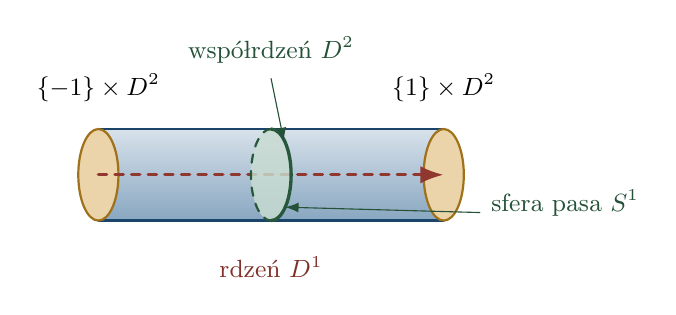
\begin{tikzpicture}[>=Latex,line cap=round,font=\small,scale=1.02]
 \shade[top color=manifoldblue!18,bottom color=manifoldblue!54]
      (-2.15,-.57) rectangle (2.15,.57);
 \draw[manifoldblue!75!black,thick]
      (-2.15,.57)--(2.15,.57)
      (-2.15,-.57)--(2.15,-.57);
 \fill[manifoldgold!39] (-2.15,0) ellipse (.25 and .57);
 \draw[manifoldgold!78!black,thick]
      (-2.15,0) ellipse (.25 and .57);
 \fill[manifoldgold!39] (2.15,0) ellipse (.25 and .57);
 \draw[manifoldgold!78!black,thick]
      (2.15,0) ellipse (.25 and .57);
 \draw[manifoldred!85!black,dashed,very thick,->]
      (-2.15,0)--(2.15,0);
 \fill[manifoldgreen!27,opacity=.82]
      (0,0) ellipse (.25 and .57);
 \draw[manifoldgreen!70!black,dashed,thick]
      (0,.57) arc[start angle=90,end angle=270,
                    x radius=.25,y radius=.57];
 \draw[manifoldgreen!70!black,very thick]
      (0,-.57) arc[start angle=270,end angle=450,
                    x radius=.25,y radius=.57];
 \node[anchor=south] at (-2.15,.79) {$\{-1\}\times D^2$};
 \node[anchor=south] at (2.15,.79) {$\{1\}\times D^2$};
 \node[manifoldgreen!65!black,anchor=south]
      at (0,1.27) {współrdzeń $D^2$};
 \draw[->,manifoldgreen!65!black]
      (0,1.20)--(.16,.42);
 \node[manifoldred!75!black] at (0,-1.15)
      {rdzeń $D^1$};
 \node[manifoldgreen!65!black,anchor=west]
      at (2.62,-.35) {sfera pasa $S^1$};
 \draw[->,manifoldgreen!65!black]
      (2.60,-.47)--(.177,-.403);
\end{tikzpicture}
\caption{Uchwyt indeksu $1$ w trójwymiarowym
kobordyzmie: dwie złote podstawy są przyczepiane
do starego brzegu. Czerwona przerywana oś jest
rdzeniem; zielony środkowy dysk jest współrdzeniem,
a jego okrąg brzegowy to sfera pasa. Rysunek
pokazuje sam uchwyt, bez reszty kobordyzmu.}
\label{fig:anatomia-uchwytu-18}
\end{figure}

\begin{twierdzenie}[Uchwyt widziany od drugiej strony]
\label{thm:dualny-uchwyt-18}
Po odwróceniu kierunku kobordyzmu uchwyt
indeksu $k$ w wymiarze $m$ staje się uchwytem
indeksu $m-k$. Jego nowym rdzeniem jest stary
współrdzeń, a nową sferą przyczepienia stara
sfera pasa. Cała lista indeksów odwraca kolejność
i zamienia $k$ na $m-k$.
\end{twierdzenie}
\begin{proof}
W modelu $F=c-|u|^2+|v|^2$ z
Lematu~\ref{thm:lemat-morsea-17}
odwrócenie funkcji daje
$-F=-c-|v|^2+|u|^2$.
Ujemna podprzestrzeń hesjanu dla $-F$
to dotychczasowa dodatnia część wymiaru
$m-k$. Zamiana miejsc czynników w
$D^k_u\times D^{m-k}_v$ daje
$D^{m-k}_v\times D^k_u$.
Jej część przyczepiana leży w brzegu,
który wcześniej był wyjściowy:
jest to $S^{m-k-1}\times D^k$.
Stąd nowa sfera przyczepienia to
$S^{m-k-1}\times\{0\}$, czyli stara
sfera pasa. Przechodzenie poziomic
od $N_+$ do $N_-$ odwraca także
porządek wszystkich punktów krytycznych.
\end{proof}

\section{Co dzieje się z brzegiem: ślad chirurgii}
\label{sec:slad-chirurgii-18}

W rozdziale poprzednim patrzyliśmy na całe
podpoziomice. Teraz chcemy zrozumieć tylko
ich \emph{brzegi}, czyli rozmaitości $N_t=F^{-1}(t)$.
Zmiana brzegu jest operacją chirurgiczną
z Definicji~\ref{def:chirurgia-zarys-16}.

\begin{twierdzenie}[Uchwyt jako ślad chirurgii]
\label{thm:slad-chirurgii-18}
Niech $1\leq k\leq m-1$ i załóżmy, że
elementarny kobordyzm $W$ powstaje z
$N_-^{m-1}\times[0,1]$ przez dołączenie
jednego $k$-uchwytu za pomocą
\[
 \alpha:S^{k-1}\times D^{m-k}
       \hookrightarrow N_-\times\{1\}.
\]
Po wygładzeniu naroży jego drugi brzeg wynosi
\begin{equation}\label{eq:brzeg-chirurgia-18}
 N_+\cong
 \bigl(N_-\setminus\operatorname{int}
        \alpha(S^{k-1}\times D^{m-k})\bigr)
 \mathop{\cup}_{S^{k-1}\times S^{m-k-1}}
       (D^k\times S^{m-k-1}).
\end{equation}
Jest to chirurgia indeksu $k-1$ na
$(m-1)$-wymiarowym $N_-$.
Odwrotnie, każda taka obramowana chirurgia
ma ślad będący elementarnym kobordyzmem
z jednym $k$-uchwytem.
\end{twierdzenie}
\begin{proof}
Brzeg uchwytu ma dwa kawałki:
\[
 \partial(D^k\times D^{m-k})
 =\underbrace{S^{k-1}\times D^{m-k}}_{A}
   \cup
   \underbrace{D^k\times S^{m-k-1}}_{B}.
\]
Kawałki spotykają się dokładnie we wspólnym
brzegu $S^{k-1}\times S^{m-k-1}$.
Podczas przyklejania $A$ zostaje utożsamiony
z $\alpha(A)$ leżącym w starym brzegu;
punkty wnętrza $A$ przestają należeć do brzegu całości.
Punkty $\partial A=\partial B$ leżą jeszcze na narożu,
które następnie wygładzamy.
Pozostała część $N_-$ nadal jest w brzegu,
a kawałek $B$ staje się \emph{nową} częścią
brzegu. To daje~\eqref{eq:brzeg-chirurgia-18}.
Żaden inny fragment $\partial H_k$ nie pozostaje.
Identyfikacja $\alpha$ obejmuje normalne dyski
$D^{m-k}$, więc zawiera dane obramowania;
bez nich wyrażenie po prawej nie jest
jednoznaczną operacją gładką.

W drugą stronę bierzemy $N_-\times[0,1]$
i przyklejamy $D^k\times D^{m-k}$ do górnego
brzegu przez zadane obramowane zanurzenie
$\alpha$. To buduje zwarty kobordyzm, którego
brzeg wyjściowy jest dokładnie prawą stroną
\eqref{eq:brzeg-chirurgia-18}. Wygładzenie
naroży odbywa się w kołnierzu wspólnego brzegu.
\end{proof}

\begin{uwaga}[Skrajne indeksy]
Przy $k=0$ nic nie przyklejamy do starego
brzegu: powstaje nowa składowa $D^m$,
której brzeg to $S^{m-1}$. Przy $k=m$
uchwyt przykleja się całym $S^{m-1}$,
zamykając odpowiednią składową brzegu.
Dlatego w~\eqref{eq:brzeg-chirurgia-18}
ograniczyliśmy się do $1\leq k\leq m-1$.
\end{uwaga}

\begin{przyklad}[Sfera przechodzi w torus]
\label{prz:sfera-torus-chirurgia-18}
Weźmy $m=3$, $k=1$ i $N_-=S^2$.
Wybierzmy przyklejenie zgodne z orientacją,
tak aby orientacja $S^2\times[0,1]$ przedłużała się
na dołączony uchwyt.
Obszar $S^0\times D^2$ to dwa rozłączne
dyski w sferze. Po usunięciu ich wnętrz
pozostaje pierścień $S^1\times[0,1]$.
Nowa część brzegu $D^1\times S^1$
jest \emph{drugim} pierścieniem; sklejenie
obu wzdłuż dwóch okręgów daje spójną, zorientowaną
powierzchnię o charakterystyce Eulera $0$, czyli $T^2$.
Identyfikację z torusem można uzasadnić bez klasyfikacji powierzchni.
Po sklejeniu jednej pary okręgów mamy dłuższy pierścień;
sklejenie jego końców opisuje dyfeomorfizm $h:S^1\to S^1$.
Orientowalność oznacza, że $h$ zachowuje orientację okręgu.
Jego podniesienie $\widetilde h:\R\to\R$ spełnia
$\widetilde h(x+1)=\widetilde h(x)+1$ oraz $\widetilde h'(x)>0$.
Dlatego $(1-t)x+t\widetilde h(x)$, $0\leq t\leq1$,
opuszcza się do izotopii $h_t$ od identyczności do $h$.
Wybierając parametr tej izotopii stały blisko końców,
otrzymujemy dyfeomorfizm
\[
 (S^1\times[0,1])/((x,1)\sim(h(x),0))\longrightarrow S^1\times S^1,
 \qquad [x,t]\longmapsto(h_t(x),e^{2\pi it}).
\]
Stałość izotopii przy końcach zapewnia gładkość po sklejeniu.
Warunek orientacji jest istotny: przy drugim typie
sklejenia pierścieni powstaje butelka Kleina,
a trójwymiarowy kobordyzm jest nieorientowalny.
Jeśli dodatkowo wypełnimy wejściowy brzeg
kulą $D^3$, powstanie $D^3$ z dołączonym
$1$-uchwytem, czyli pełny torus $D^2\times S^1$.
Sam kobordyzm ma \emph{dwa} brzegi: $S^2$ i $T^2$.
Zgodność charakterystyk Eulera kontroluje
wynik: $\chi(S^2)=2$, usuwamy dwa dyski
o łącznej charakterystyce $2$ i wklejamy
pierścień o charakterystyce $0$, więc
$\chi(T^2)=0$. To sprawdzenie nie zastępuje
opisu sposobu sklejenia.
\end{przyklad}

\begin{figure}[htbp]
\centering
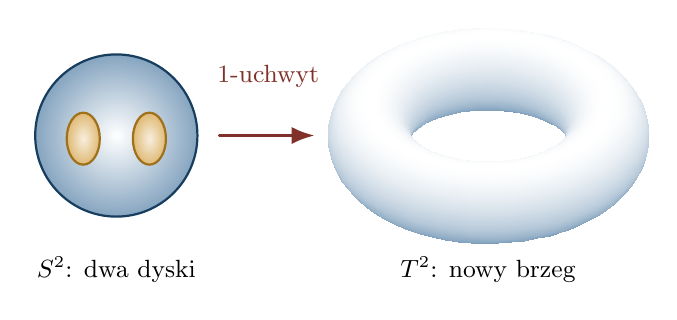
\begin{tikzpicture}[>=Latex,line cap=round,font=\small]
 % Lewy brzeg: sfera z dwoma zaznaczonymi dyskami.
 \shade[inner color=white,outer color=manifoldblue!55]
      (-3.12,0) circle (1.03);
 \draw[manifoldblue!68!black,thick] (-3.12,0) circle (1.03);
 \shade[inner color=manifoldgold!15,outer color=manifoldgold!63]
      (-3.54,-.04) ellipse (.21 and .33);
 \shade[inner color=manifoldgold!15,outer color=manifoldgold!63]
      (-2.70,-.04) ellipse (.21 and .33);
 \draw[manifoldgold!78!black,thick]
      (-3.54,-.04) ellipse (.21 and .33)
      (-2.70,-.04) ellipse (.21 and .33);
 \node at (-3.12,-1.70) {$S^2$: dwa dyski};
 \draw[->,very thick,manifoldred!75!black]
       (-1.81,0)--(-.60,0);
 \node[align=center,manifoldred!75!black] at (-1.19,.75)
       {$1$-uchwyt};
 % Prawy brzeg: gładki model parametryczny torusa.
 \begin{scope}[shift={(1.60,0)}]
   \begin{axis}[hide axis,view={0}{34},axis equal image,scale=2,
      xmin=-3,xmax=3,ymin=-3,ymax=3,zmin=-.8,zmax=.8,scale only axis,
      at={(0,0)},anchor=center,width=9cm,height=5cm,
       colormap={toruslight}{color(0cm)=(manifoldblue!67);
         color(.42cm)=(manifoldblue!33);color(1cm)=(white)}]
    \addplot3[surf,shader=interp,draw=none,z buffer=sort,
      samples=34,samples y=68,domain=0:360,y domain=0:360,
      variable=\t,variable y=\p]
     ({(2+0.69*cos(\t))*cos(\p)},
      {(2+0.69*cos(\t))*sin(\p)},
      {0.69*sin(\t)});
   \end{axis}
 \end{scope}
 \node at (1.60,-1.70) {$T^2$: nowy brzeg};
\end{tikzpicture}
\caption{Dołączenie $1$-uchwytu zgodnie z orientacją zmienia
brzeg wyjściowy trójwymiarowego kobordyzmu z $S^2$ na $T^2$.
Zaznaczone na sferze złote dyski stanowią
$S^0\times D^2$; po wycięciu ich wnętrz
doklejamy pierścień $D^1\times S^1$.}
\label{fig:chirurgia-sfera-torus-18}
\end{figure}

\begin{przyklad}[Operacja odwrotna i dualny uchwyt]
Odwróćmy poprzedni kobordyzm. Ten sam
trójwymiarowy kawałek widzimy teraz jako
$2$-uchwyt przyczepiony do torusa.
W pośrednim $T^2$ sfera pasa wcześniejszego
$1$-uchwytu jest okręgiem \emph{południkowym}.
Przy odwróceniu kobordyzmu właśnie ona staje się
sferą przyczepienia dualnego $2$-uchwytu,
zgodnie z Twierdzeniem~\ref{thm:dualny-uchwyt-18}.
Wzór~\eqref{eq:brzeg-chirurgia-18}
opisuje przejście $T^2\to S^2$ jako
chirurgię indeksu $1$. Obramowanie tej
krzywej jest tutaj odziedziczone po pierwszym uchwycie.
Ogólnie przyklejenie określa obramowane pogrubienie,
a nie tylko obraz sfery przyczepienia.
\end{przyklad}

\section{Łańcuchy uchwytów i liczby przecięcia}
\label{sec:lancuchy-uchwytow-18}

Uchwyt jest pogrubioną komórką. Z tego powodu
rozkład~\eqref{eq:rozklad-kobordyzm-18} powinien
prowadzić do kompleksu obliczającego homologię
\emph{względną} $H_*(W,N_-)$. Ważna nowość
polega na tym, że jego różniczkę można odczytać
z przecięcia dwóch sfer w poziomicy.

\begin{twierdzenie}[Kompleks względny uchwytów]
\label{thm:kompleks-uchwytow-18}
Załóżmy, że uchwyty ułożono według indeksów,
tak że wszystkie uchwyty indeksu $k-1$
przyczepiono przed uchwytami indeksu $k$.
Taki porządek można osiągnąć ruchem opisanym
w Twierdzeniu~\ref{thm:przestawianie-18}.
Po wybraniu orientacji rdzeni istnieje kompleks
\[
 C_k(W,N_-)=\Z\langle
       \text{uchwyty indeksu }k\rangle,
 \qquad H_k(C_\bullet,\partial)\cong H_k(W,N_-;\Z).
\]
Jeśli $p$ jest $k$-uchwytem, a $q$ jest
$(k-1)$-uchwytem, to współczynnik przy $q$
w $\partial_k p$ jest podpisaną liczbą
poprzecznych przecięć w pośredniej poziomicy:
\begin{equation}\label{eq:macierz-uchwyty-18}
 \langle\partial_kp,q\rangle
 = I\bigl(A_p,B_q\bigr),\qquad
 A_p=S^{k-1}\times\{0\},\quad
 B_q=\{0\}\times S^{m-k}.
\end{equation}
Sfery przenosimy do tej samej poziomicy
przez regularne pasy przepływem.
\end{twierdzenie}
\begin{proof}
Niech $W^{(k)}$ będzie częścią po dołączeniu
uchwytów indeksów co najwyżej $k$,
a $W^{(-1)}=N_-$ wraz z małym kołnierzem.
Wycięcie pozostałej przestrzeni i
ściągnięcie drugiego czynnika każdego
$D^k\times D^{m-k}$ dają
\[
 H_j(W^{(k)},W^{(k-1)};\Z)
 \cong
 \bigoplus_{p:\,\lambda(p)=k}
 H_j(D^k,S^{k-1};\Z)
 =
 \begin{cases}
 \Z^{c_k},&j=k,\\
 0,&j\ne k.
 \end{cases}
\]
Dla uchwytów tego samego indeksu wybieramy pole
Morse'a--Smale'a; nie ma między nimi trajektorii.
Ich sfery wyjściowe można więc sprowadzić do jednego
poziomu poniżej całego bloku. Czasy trafienia są
gładkie i ograniczone na tych zwartych sferach;
inaczej granica dałaby trajektorię do punktu
o tym samym indeksie. Sfery są rozłączne, gdyż
trajektoria ma tylko jeden początek krytyczny.
Ich dostatecznie małe pogrubienia też są rozłączne.
Pozwala to dołączyć cały blok jednocześnie
i uzasadnia powyższą sumę prostą przez wycięcie
po uprzednim pogrubieniu części przyczepianych kołnierzami.
Orientacja dysku rdzenia wybiera generator
odpowiedniego składnika $\Z$.

Różniczka jest złożeniem
\[
 H_k(W^{(k)},W^{(k-1)})
 \xrightarrow{\delta}H_{k-1}(W^{(k-1)},N_-)
 \longrightarrow H_{k-1}(W^{(k-1)},W^{(k-2)}).
\]
Pierwsze odwzorowanie pochodzi z ciągu dokładnego trójki
$(W^{(k)},W^{(k-1)},N_-)$, a drugie zapomina
część względną. W stopniu $0$ brzeg jest zerowy.
Jego kwadrat jest zerowy: brzeg brzegu
rdzenia znika, co można też sprawdzić
w długich ciągach dokładnych kolejnych
potrójek. Ponieważ każda para
$(W^{(k)},W^{(k-1)})$ ma homologię
skupioną w jednym stopniu, kolejne
długie ciągi dokładne, albo równoważny
kompleks CW z
Twierdzenia~\ref{thm:cw-morse-17},
identyfikują homologię tego kompleksu
z $H_*(W,N_-)$.

Pozostaje uzasadnić konkretny wzór.
Brzeg zorientowanego rdzenia $p$
to jego sfera przyczepienia $A_p$.
Przenosimy ją do regularnej poziomicy,
w której widoczny jest współrdzeń $q$.
Po zgnieceniu innych komórek niż $q$
współczynnik brzegowy jest stopniem
odwzorowania
$S^{k-1}\to S^{k-1}$.
Wybieramy wartość regularną w komórce $q$.
Jej przeciwobrazy odpowiadają dokładnie
przecięciom $A_p$ ze sferą pasa $B_q$:
współrdzeń $q$ jest poprzecznym dyskiem,
a jego brzeg leży w rozważanej poziomicy.
Orientujemy $A_p$ jako brzeg rdzenia $p$.
Normalną orientację $B_q$ wyznacza zorientowany
rdzeń $q$: w modelu uchwytu jego kierunki są
normalne do współrdzenia. Znak przecięcia to znak
izomorfizmu $T_zA_p\to\nu_z B_q$ w poziomicy.
Jest on znakiem lokalnego stopnia. Ta konwencja
działa także dla nieorientowalnego $W$ i zgadza się
z konwencją w dowodzie
Twierdzenia~\ref{thm:homologia-morse-17}.
Sumując znaki, otrzymujemy
\eqref{eq:macierz-uchwyty-18}.
Zmiana orientacji rdzenia zmienia tylko
znak odpowiedniego generatora.
\end{proof}

\begin{przyklad}[Jeden punkt przecięcia lub żaden]
\label{prz:meridian-longitude-18}
Zacznijmy od $S^2\times[0,1]$ i
dołączmy $1$-uchwyt, otrzymując na górze $T^2$.
Jego sfera pasa $B_1$ jest południkiem
torusa. Jeżeli kolejny $2$-uchwyt przyczepimy
wzdłuż krzywej biegnącej raz w kierunku
równoleżnikowym, to sfera przyczepienia
$A_2$ przecina $B_1$ w jednym punkcie.
Po dobraniu orientacji
$C_2=\Z\xrightarrow{\ \partial_2=\pm1\ }
 C_1=\Z$.
Kompleks względny jest acykliczny,
a geometryczne zniesienie pary
udowodnimy w
Twierdzeniu~\ref{thm:zniesienie-18}.

Jeśli natomiast przyczepimy $2$-uchwyt
wzdłuż krzywej \emph{równoległej do
południka} $B_1$, po małej perturbacji
krzywe te są rozłączne i $\partial_2=0$.
To inny wybór niż w parze znoszącej się.
W odwróconym pojedynczym kobordyzmie
z poprzedniego przykładu południk
jest właśnie sferą przyczepienia
\emph{dualnego} $2$-uchwytu;
nie należy mylić tych dwóch sytuacji.
\end{przyklad}

\begin{figure}[htbp]
\centering
\begin{tikzpicture}[>=Latex,font=\small,line cap=round,scale=1.15]
 \fill[manifoldblue!6] (-1.45,-1.15) rectangle (1.45,1.15);
 \draw[manifoldblue!70!black,thick]
      (-1.45,-1.15) rectangle (1.45,1.15);
 \draw[manifoldgreen!70!black,very thick,->]
      (0,-1.15)--(0,.85);
 \draw[manifoldgreen!70!black,very thick]
      (0,.85)--(0,1.15);
 \draw[manifoldred!82!black,very thick,->]
      (-1.45,0)--(1.18,0);
 \draw[manifoldred!82!black,very thick]
      (1.18,0)--(1.45,0);
 \fill[manifoldgold!85!black] (0,0) circle (2.5pt);
 \node[manifoldgreen!65!black,anchor=west] at (.12,.78)
       {$B_1$};
 \node[manifoldred!80!black,anchor=south] at (.95,.09)
       {$A_2$};
 \node[anchor=north,align=center] at (0,-1.35)
       {przeciwległe boki są sklejone: $T^2$};
\end{tikzpicture}
\caption{Pośredni torus przedstawiony jako kwadrat
ze sklejonymi bokami. Zielona sfera pasa
$B_1$ i czerwona sfera przyczepienia
$A_2$ przecinają się raz. Dlatego odpowiedni
współczynnik macierzy $\partial_2$ wynosi
$+1$ albo $-1$, zależnie od orientacji.}
\label{fig:przeciecie-uchwytow-18}
\end{figure}

\begin{uwaga}[Rachunek algebraiczny to jeszcze nie geometria]
Jeżeli współczynnik
$\langle\partial_{k+1}p,q\rangle=\pm1$,
to po zmianach baz można wydzielić podkompleks
$0\to\Z\xrightarrow{\pm1}\Z\to0$ i go usunąć.
Najpierw zerujemy pozostałe wpisy w wierszu i kolumnie
tego współczynnika. Tożsamość $\partial^2=0$
zeruje wówczas odpowiednie wpisy w sąsiednich
różniczkach, więc naprawdę otrzymujemy sumę prostą
kompleksów. Usunięty składnik jest ściągalny.
Nie wynika z tego automatycznie, że
sfery $A_p$ i $B_q$ mają \emph{jeden
geometryczny} punkt przecięcia:
podpisana suma może wynosić $1$
przy trzech, pięciu albo większej
liczbie punktów. Ich usunięcie wymaga
argumentu geometrycznego, często
triku Whitneya i warunków wymiarowych.
\end{uwaga}

\section{Przestawianie i przesuwanie uchwytów}
\label{sec:ruchy-uchwytow-18}

Lista uchwytów zależy od funkcji Morse'a,
choć sam kobordyzm pozostaje ten sam.
Dwa podstawowe ruchy mają różne znaczenie:
\emph{przestawienie} zmienia kolejność
wartości krytycznych, a \emph{przesunięcie}
(ang.\ \emph{handle slide}) zmienia sposób
przyczepienia uchwytów tego samego indeksu.

\begin{definicja}[Pole gradientopodobne spadku]
\index{pole gradientopodobne spadku@Pole gradientopodobne spadku}
\label{def:pole-spadku-18}
Przez pole gradientopodobne dla $F$ rozumiemy pole $X$
spełniające $XF<0$ poza punktami krytycznymi,
zerujące się w tych punktach i będące blisko każdego
z nich ujemnym gradientem $F$ dla pewnej gładkiej metryki.
Można wybrać $X=-\nabla_g F$ na całym kobordyzmie,
z metryką euklidesową w małych mapach Morse'a.
W kołnierzach $X$ jest skierowane od wyjścia do wejścia.
\end{definicja}

Poza zerami takie pole również można zrealizować
jako ujemny gradient: ustalamy
$g(X,X)=-\dd F(X)>0$, $g(X,\ker\dd F)=0$
i dodatnią metrykę na $\ker\dd F$.
Podział jedności skleja te metryki z ustalonymi
przy zerach, zachowując $g(X,\cdot)=-\dd F$.
W konsekwencji wcześniejsze argumenty o końcach
trajektorii stosują się aż do chwili trafienia w brzeg.

\begin{twierdzenie}[Przestawianie dwóch punktów]
\label{thm:przestawianie-18}
Niech $p,q$ będą jedynymi punktami krytycznymi
pewnego pasa, $F(p)<F(q)$.
Jeżeli dla wybranego gradientopodobnego pola
spadku nie ma trajektorii $q\to p$,
można zmienić $F$ we wnętrzu tego pasa
bez tworzenia nowych punktów krytycznych,
tak aby $p$ i $q$ zamieniły kolejność wartości.
Pole $X$ można zachować na \emph{całym} paśmie:
$X\widetilde F<0$ poza jego zerami, a blisko $p,q$
nowa funkcja różni się od starej tylko o stałe.
Przy brzegach pasa funkcja pozostaje niezmieniona.
W szczególności
rozkład uchwytowy można uporządkować
według niemalejących indeksów.
\end{twierdzenie}
\begin{proof}
Niech pas ma regularne końce $a<b$ i wybierzmy
$F(p)<s<F(q)$, $L=F^{-1}(s)$.
Zbiory $A=W^s(p)\cap L$ i $B=W^u(q)\cap L$
są rozłączne: punkt wspólny dawałby trajektorię $q\to p$.
Są też zwarte. Na przykład mała sfera wejściowa
lokalnego dysku stabilnego $p$ po przepływie wstecz
dociera do $L$, ponieważ między jej poziomem a $s$
nie ma punktów krytycznych. Czas trafienia jest
gładki na zwartej sferze, a jej obraz to $A$.
Tak samo otrzymujemy $B$ z lokalnej sfery niestabilnej $q$.
Zbiór może być pusty przy skrajnym indeksie.

Wybierzmy gładką $\rho_L:L\to[0,1]$, równą $1$
w otoczeniu $A$ i $0$ w otoczeniu $B$.
Przedłużmy ją na całe pasmo, nadając tę samą wartość
wszystkim punktom jednej trajektorii przecinającej $L$.
Trajektorie poniżej $L$, które nie przecinają $L$
wstecz, muszą mieć początek w $p$; na nich kładziemy $\rho=1$.
Trajektorie powyżej $L$, które nie dochodzą do $L$
naprzód, muszą kończyć się w $q$; na nich kładziemy $\rho=0$.
Tak samo definiujemy wartości w samych $p,q$.

Sprawdźmy gładkość tego przedłużenia.
Tam, gdzie trajektoria przecina $L$ w skończonym czasie,
wynika ona z gładkości czasu trafienia.
W dostatecznie małym otoczeniu $p$ wszystkie trajektorie,
które dochodzą do $L$ wstecz, trafiają w obszar $\rho_L=1$.
Gdyby nie, ciąg punktów dążących do $p$ dawałby
po wybraniu podciągu punkt graniczny na $L$ poza tym obszarem.
Jego trajektoria musiałaby zbiegać do $p$:
w przeciwnym razie dochodziłaby do dolnego brzegu
w skończonym czasie, podobnie jak pobliskie trajektorie,
zanim mogłyby zbliżyć się do $p$.
To przeczyłoby temu, że cały $A$ leży w obszarze $\rho_L=1$.
Zatem $\rho$ jest identycznie $1$ blisko $p$.
Jest też stała w otoczeniu każdego dalszego punktu
$W^u(p)$, po przeniesieniu tego otoczenia przepływem.
Analogicznie $\rho=0$ blisko $q$ i wzdłuż $W^s(q)$.
Otrzymujemy gładką funkcję na całym paśmie z $X\rho=0$.

Wybierzmy rosnące dyfeomorfizmy $h_p,h_q:[a,b]\to[a,b]$,
równe identyczności przy końcach, takie że
\[
 h_p(F(p))>h_q(F(q)).
\]
W małym otoczeniu odpowiedniej wartości krytycznej
każdy $h$ może być translacją. Takie odwzorowania konstruujemy,
zadając dodatnią pochodną o odpowiednich całkach
na przedziałach po obu stronach tej wartości.
Nie próbujemy przestawić dwóch liczb jednym odwzorowaniem rosnącym:
używamy dwóch różnych odwzorowań na różnych rodzinach trajektorii.
Kładziemy
\[
 \widetilde F=\rho\,h_p(F)+(1-\rho)h_q(F).
\]
Wtedy
\[
 X\widetilde F=
 \bigl(\rho h_p'(F)+(1-\rho)h_q'(F)\bigr)XF<0
\]
poza $p,q$, więc nowe punkty krytyczne nie powstają.
Blisko $p$ lub $q$ dodaliśmy tylko stałą,
zachowując hesjany i indeksy. Przy końcach pasa
oba odwzorowania $h$ są identycznością, więc także $\widetilde F=F$.
To dowodzi przestawienia przy niezmienionym polu.

Dla ostatniego zdania wybieramy
pole Morse'a--Smale'a jak w
Twierdzeniu~\ref{thm:gen-ms-17}.
Wtedy trajektoria od $q$ do $p$
wymaga $\lambda(q)>\lambda(p)$
(Stwierdzenie~\ref{prop:wymiar-ms-17}).
Jeśli dwa sąsiednie punkty, wymienione od niższej
do wyższej wartości funkcji, mają indeksy
w kolejności malejącej lub równej,
takiej trajektorii nie ma i wolno je
zamienić. Kolejne zamiany, jak przy
porządkowaniu skończonej listy, ustawiają
indeksy niemalejąco.
\end{proof}

\begin{uwaga}
Warunek o trajektorii jest istotny.
Jeśli $q\to p$ istnieje, przepływ
łączy dwa lokalne modele i niezależne
przesunięcie ich wartości może
przestać być zgodne z kierunkiem
spadku. Powyższe twierdzenie nie
pozwala dowolnie przestawiać wszystkich
uchwytów.
\end{uwaga}

\begin{stwierdzenie}[Przesunięcie uchwytu]
\label{prop:slide-18}
Załóżmy, że $p$ i $q$ są dwoma uchwytami
tego samego indeksu $1\leq k\leq m-1$,
przyczepionymi w jednym bloku rozkładu.
Dla $k\geq2$ wybieramy obramowaną wstęgę od sfery
przyczepienia $p$ do małej równoległej kopii sfery $q$,
wyznaczonej przez obramowanie uchwytu $q$.
Wnętrze wstęgi omija wszystkie sfery i ich używane
pogrubienia. Sferę $p$ zastępujemy sumą połączoną
z tą kopią; sam uchwyt $q$ pozostaje na miejscu.
Zakładamy istnienie takiej wstęgi z uzgodnionym
obramowaniem, nie dowolnego łuku przecinającego inne dane.
Dla $k=1$ przesuwamy jedną ze stóp
uchwytu $p$ przez uchwyt $q$.
Cały kobordyzm pozostaje dyfeomorficzny
względem brzegu wejściowego $N_-$.
W kompleksie z
Twierdzenia~\ref{thm:kompleks-uchwytow-18}
ruch ten jest elementarną zmianą bazy
\begin{equation}\label{eq:slide-baza-18}
 e_p'=e_p\pm e_q,\qquad e_q'=e_q.
\end{equation}
\end{stwierdzenie}
\begin{proof}
Przyczepmy najpierw uchwyt $q$.
W jego nowym brzegu $D^k\times S^{m-k-1}$
wybierzmy $v_0\in S^{m-k-1}$.
Równoległa kopia $S^{k-1}\times\{v_0\}$ dawnej
sfery przyczepienia ogranicza teraz dysk
$D^k\times\{v_0\}$ leżący \emph{w brzegu}.
Dysk ten jest równoległy do rdzenia; nie prowadzimy
izotopii po rdzeniu leżącym we wnętrzu kobordyzmu.
Dla $k\geq2$ sumę połączoną z brzegiem tego dysku
można zsunąć przez dysk na pierwotną sferę $p$.
W jego produktowym otoczeniu jest to zwykłe
przesunięcie paska, wraz z normalnym pogrubieniem.
Założenie o obramowanej wstędze zapewnia zgodność
tego pogrubienia po obu stronach.
Dla $k=1$ dysk jest odcinkiem i przesuwamy
jedną stopę uchwytu wzdłuż tego odcinka.

Jest to izotopia obramowanego przyklejenia $p$
w brzegu przestrzeni z już dołączonym $q$.
Twierdzenie o przedłużaniu izotopii z
Sekcji~\ref{sec:izotopie-otoczen-15} rozszerza ją
na otoczenie brzegu, z nośnikiem poza wcześniejszym
brzegiem wejściowym. Przedłużenie na uchwyt $p$
daje dyfeomorfizm dwóch rozkładów względem $N_-$.
Nie musi on punktowo unieruchamiać całej wcześniej
dołączonej części wraz z jej brzegiem wyjściowym.
Jeśli dołączono dalsze uchwyty, przenosimy także
ich odwzorowania przyczepienia przez ten dyfeomorfizm.

Prześledźmy rdzeń $D^k$ uchwytu $p$
przez ten ruch. Jego nowa klasa
w grupie względnej
$H_k(W^{(k)},W^{(k-1)})$
biegnie raz przez dawny rdzeń $p$
i raz, ze znakiem zależnym od
orientacji wstęgi, przez rdzeń $q$.
Pozostałe rdzenie nie są dotknięte.
To daje~\eqref{eq:slide-baza-18}.
Ponieważ $\partial$ jest liniowy,
$\partial_k e_p'
 =\partial_k e_p\pm\partial_k e_q$.
Jeśli występują uchwyty indeksu $k+1$,
ich współrzędne w stopniu $k$ zmieniają
się przez odwrotną zmianę bazy;
homologia pozostaje ta sama.
\end{proof}

\begin{figure}[htbp]
\centering
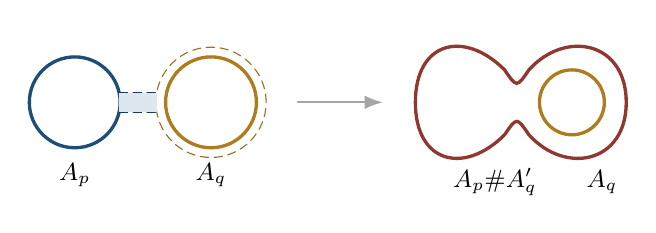
\begin{tikzpicture}[>=Latex,font=\small,line cap=round,scale=1.03]
 \draw[manifoldblue!85!black,very thick]
      (-3.35,0) circle (.56);
 \draw[manifoldgold!85!black,very thick]
      (-1.67,0) circle (.56);
 \draw[manifoldgold!75!black,densely dashed]
      (-1.67,0) circle (.68);
 \fill[manifoldblue!15]
      (-2.80,-.12)--(-2.34,-.12)
      --(-2.34,.12)--(-2.80,.12)--cycle;
 \draw[manifoldblue!65!black,densely dashed]
      (-2.80,-.12)--(-2.34,-.12)
      (-2.80,.12)--(-2.34,.12);
 \node at (-3.35,-.90) {$A_p$};
 \node at (-1.67,-.90) {$A_q$};
 \draw[->,gray!70,thick] (-.60,0)--(.45,0);
 \draw[manifoldred!85!black,very thick]
      (.85,0) .. controls (.85,.75) and (1.45,.90)
      .. (1.95,.40) .. controls (2.10,.18) and (2.10,.18)
      .. (2.25,.40) .. controls (2.70,.90) and (3.45,.75)
      .. (3.45,0) .. controls (3.45,-.75) and (2.70,-.90)
      .. (2.25,-.40) .. controls (2.10,-.18) and (2.10,-.18)
      .. (1.95,-.40) .. controls (1.45,-.90) and (.85,-.75)
      .. (.85,0);
 \draw[manifoldgold!85!black,very thick]
      (2.78,0) circle (.40);
 \node at (1.83,-.98) {$A_p\# A_q'$};
 \node at (3.15,-.98) {$A_q$};
\end{tikzpicture}
\caption{Schemat przesunięcia w przypadku,
gdy sfery przyczepienia są okręgami.
Po lewej wybieramy wstęgę między
$A_p$ i przerywaną równoległą kopią $A_q'$ sfery $A_q$;
sam złoty okrąg $A_q$ pozostaje na miejscu.
Po prawej nowa sfera
przyczepienia pierwszego uchwytu
przebiega raz także wzdłuż drugiego.
Dokładne zanurzenie i obramowanie
w wyższym wymiarze nie są tu pokazane.}
\label{fig:slide-18}
\end{figure}

\section{Kiedy dwa uchwyty naprawdę się znoszą?}
\label{sec:znoszenie-uchwytow-18}

Na poziomie algebry różniczka $1:\Z\to\Z$
ma jądro i koker zerowe. Geometrycznie
potrzebujemy czegoś mocniejszego: dwie
odpowiednie sfery muszą spotkać się
\emph{w jednym punkcie}, a nie tylko
z algebraiczną sumą znaków równą $1$.

\begin{twierdzenie}[Geometryczne zniesienie pary]
\label{thm:zniesienie-18}
Niech pas kobordyzmu zawiera dokładnie
dwa punkty krytyczne $p,q$ o indeksach
odpowiednio $k,k+1$ i wartościach
$F(p)<F(q)$. Załóżmy, że dla wybranego
pola gradientopodobnego sfera przyczepienia
$A_q$ przecina sferę pasa $B_p$ w jednej
regularnej poziomicy \emph{poprzecznie
w dokładnie jednym punkcie}.
Wtedy można zmienić funkcję Morse'a
we wnętrzu pasa, nie ruszając jej przy
jego brzegach, tak by nie miała w nim
punktów krytycznych. Pas jest zatem
iloczynowym kobordyzmem: para uchwytów
$H_k,H_{k+1}$ znosi się.
\end{twierdzenie}
\begin{proof}
\emph{Krok 1: jedna trajektoria.}
Każda trajektoria z $q$ do $p$ przecina
każdą regularną poziomicę między ich
wartościami dokładnie raz, bo $F$
ściśle maleje poza punktami krytycznymi.
Punkt przecięcia $A_q\cap B_p$ wyznacza
taką trajektorię. Przy jednym punkcie
przecięcia jest więc dokładnie jedna
trajektoria łącząca, oznaczmy ją $\gamma$.
Jej przecięcie jest poprzeczne, zatem
nie znika przy małej zmianie przekroju.

\emph{Krok 2: dostosowujemy modele przy końcach.}
Nie zakładamy, że dowolny gradient da się gładko
zlinearyzować. Wolno nam natomiast zmieniać pole
spadku, zachowując funkcję i potrzebne dyski.
Przy $q$ zachowamy lokalny dysk $W^u(q)$,
a przy $p$ lokalny dysk $W^s(p)$.
Wyjaśnijmy wersję lematu Morse'a dostosowaną do takiego dysku.
Gradient jest do niego styczny. We współrzędnych
tubularnych opartych na normalnej ortogonalnej do dysku
różniczka funkcji w kierunku normalnym znika na dysku.
Taylor w zmiennej normalnej daje zatem
\[
 F(z,w)=F(z,0)+w^{\mathsf T}C(z,w)w.
\]
Przy dysku niestabilnym $C$ jest dodatnio określona,
a $F(z,0)$ ma niezdegenerowane maksimum.
Lemat Morse'a na dysku i zamiana $w\mapsto C(z,w)^{1/2}w$
dają standardowy model, zachowując dysk $w=0$.
Przy dysku stabilnym znaki są odwrotne.
W tych mapach zastępujemy pole standardowym polem
spadku, sklejonym ze starym za pomocą funkcji odcinającej.
Wypukłe połączenie dwóch pól z $XF<0$ nadal obniża $F$.
Oba pola są styczne do zachowywanego dysku, więc jego
ślad poza małym otoczeniem punktu krytycznego się nie zmienia.
W szczególności zachowujemy jedyne przecięcie $A_q\cap B_p$.

Modelem dla całej pary będzie
\begin{equation}\label{eq:narodziny-uchwytow-18}
 G_s(t,x,y)=\frac{t^3}{3}-st-|x|^2+|y|^2,
 \quad x\in\R^k,\quad y\in\R^{m-k-1}.
\end{equation}
Po dodatniej normalizacji afinicznej wartości funkcji
modele przy $p,q$ identyfikujemy z otoczeniami dwóch
punktów krytycznych $G_{s_0}$, gdzie $s_0>0$.
Stosując powyższe sklejenie, możemy tam od razu
wybrać pole odpowiadające $-\nabla G_{s_0}$.

\emph{Krok 3: uzgadniamy przejście przez regularny pas.}
Małe przekroje poniżej $q$ i powyżej $p$ łączy
dyfeomorfizm $h$ wyznaczony przepływem.
W modelu $G_{s_0}$ mamy analogiczny dyfeomorfizm $h_0$.
Po identyfikacji przekrojów ich różnicę opisuje lokalny
dyfeomorfizm $j$ przestrzeni $\R^k\times\R^{m-k-1}$,
ustalający $0$. Warunek transwersalności oznacza,
że $j(\R^k\times\{0\})$ jest poprzeczny do
$\{0\}\times\R^{m-k-1}$ w zerze.
Na małym dysku rodzina $j_\tau(z)=\tau^{-1}j(\tau z)$,
uzupełniona przez $j_0=Dj_0$, jest gładką izotopią
do części liniowej. Gładkość przy $\tau=0$ wynika ze wzoru
$j_\tau(z)=\int_0^1 Dj(t\tau z)z\,\dd t$.

Także dopasowanie części liniowej wymaga uzasadnienia.
Niech $Dj_0=\left(\begin{smallmatrix}A&B\\C&D\end{smallmatrix}\right)$.
Transwersalność daje odwracalność $A$, a odwracalność
$Dj_0$ daje odwracalność $S=D-CA^{-1}B$.
Mamy rozkład
\[
 Dj_0=
 \begin{pmatrix}I&0\\CA^{-1}&I\end{pmatrix}
 \begin{pmatrix}A&0\\0&S\end{pmatrix}
 \begin{pmatrix}I&A^{-1}B\\0&I\end{pmatrix}.
\]
Ścinania zewnętrzne kurczymy liniowo do identyczności.
Odbicia wybranych osi w mapach modelowych pozwalają
uzgodnić znaki wyznaczników $A,S$; nie zmieniają funkcji $G_s$.
Następnie łączymy oba bloki z identycznością w
$\operatorname{GL}^+$ (rozkład polarny i spójność grupy
obrotów). Cała droga zachowuje odwracalność bloku $A$,
a więc transwersalność. Bloki wymiaru zero pomijamy.

Izotopię lokalizujemy, mnożąc jej pole generujące
przez funkcję odcinającą. Kontrolujemy przy tym
\emph{całe} przecięcie, nie tylko różniczkę w zerze.
Na dostatecznie małym dysku, jednostajnie w parametrze,
\[
 \operatorname{dist}(j_\tau(u,0),\{0\}\times\R^{m-k-1})
       \geq c|u|,\qquad |V_\tau(z)|\leq C|z|.
\]
Pierwsza nierówność wynika z jednostajnej odwracalności
bloku poprzecznego, druga z $V_\tau(0)=0$.
Dzielimy izotopię na skończenie wiele dostatecznie
krótkich kroków. W każdym kroku odcięte pole zgadza się
z właściwym polem na mniejszym dysku i znika poza większym.
Czas kroku wybieramy tak, aby przesunięcie w pierścieniu
było mniejsze niż połowa dolnego oszacowania odległości.
Wtedy poza zerem nie powstaje żadne nowe przecięcie.
Kolejne mniejsze dyski wybieramy tak, aby ich obrazy
pozostawały w obszarze zgodności poprzedniego kroku.
Po skończonej liczbie kroków nowe odwzorowanie przejścia
zgadza się z $h_0$ blisko zera, a poza większym dyskiem
ze starym odwzorowaniem.

Realizujemy tę izotopię przez zmianę pola w regularnym paśmie.
We współrzędnej czasu $u=-F$ stare znormalizowane pole
jest $\partial_u$. Dodanie do niego pola stycznego
do przekrojów, generującego wybraną izotopię,
nie zmienia równości $XF=-1$.
Parametr izotopii wybieramy stały przy końcach pasa.
Nowe pole skleja się więc ze starym i nadal jest polem
spadku; jego odwzorowanie przejścia to wymagane $h_0$.
Przedłużając współrzędne przez przepływ, otrzymujemy
na otoczeniu całej trajektorii model $-\nabla G_{s_0}$
z dokładnością do dodatniej zmiany szybkości.
To wymagało zmiany pola, nie wynikało z samego
lematu Morse'a dla pierwotnego gradientu.

Dla ustalonego $s=s_0>0$ model ma dwa punkty:
$t=-\sqrt{s_0}$ o indeksie $k+1$
i $t=\sqrt{s_0}$ o indeksie $k$.
Wzdłuż osi $x=y=0$ ujemny gradient
spełnia $\dot t=s_0-t^2$ i biegnie
od pierwszego punktu do drugiego.
Każda inna trajektoria ma niezerową
składową $x$ albo $y$ i nie może mieć
obu tych końców; jest to jedyna
trajektoria łącząca.

Potrzebna jest jeszcze kontrola powrotów poza ten model.
Dla dostatecznie małego otoczenia $U$ domkniętej trajektorii
$\gamma\cup\{p,q\}$ istnieje mniejsze $V$, którego domknięcie
leży w $U$, takie że stara trajektoria wychodząca z $V$
i opuszczająca $U$ nie wraca do $V$.
Gdyby nie, istniałby ciąg odcinków wychodzących
z punktów dążących do tego łuku, przechodzących poza $U$
i ponownie zbliżających się do łuku.
Po wybraniu punktu granicznego poza $U$ otrzymalibyśmy
inną trajektorię od $q$ do $p$.
Dokładniej: gdyby jej koniec lub początek leżał
w brzegu pasa, gładka zależność i skończony czas
trafienia zmuszałyby do tego także pobliskie odcinki.
Nie mogłyby one mieć obu końców blisko wewnętrznego łuku.
Jedynymi możliwymi końcami krytycznymi są $q,p$,
a ścisły spadek wyklucza powrót do tego samego punktu.
Otrzymana druga trajektoria przeczy założeniu.
Argument stosujemy do pola \emph{po} uzgodnieniu modeli;
właśnie dlatego zachowaliśmy jedno przecięcie w całej izotopii.

\emph{Krok 4: usuwamy zera pola.}
Po pomnożeniu pola spadku przez
dodatnią funkcję jego trajektorie
w modelowej rurze są trajektoriami
\[
 X=(s_0-t^2,\,2x,\,-2y).
\]
Wybierzmy funkcję $v_1(t)<0$,
która zgadza się z $s_0-t^2$
blisko obu końców rury
($|t|>\sqrt{s_0}$), a różnicę podpieramy
w rzucie mniejszego otoczenia $V$. Niech
$\rho(r)=1$ dla bardzo małych
$r\geq0$ i $\rho(r)=0$ przy
brzegu małego przekroju, tak aby nośnik całej
zmiany był zawarty w $V$. Kładziemy
\[
 v(t,r)=\rho(r)v_1(t)
       +(1-\rho(r))(s_0-t^2),\qquad
 \widetilde X=
 \bigl(v(t,|x|^2+|y|^2),\,2x,\,-2y\bigr).
\]
Pole $\widetilde X$ jest równe $X$
przy brzegu rury i nigdzie nie
znika: dla $(x,y)\ne(0,0)$ jedna
ze składowych poprzecznych jest
niezerowa, a na osi $v=v_1<0$.
Przedłużamy je starym polem na cały pas.
Pole zmieniliśmy tylko w $V$, a wzory modelowe
obowiązują w większym $U$. Trajektoria nie może
pozostać w $U$ przez nieskończony czas
w przyszłości: wtedy z równania
$\dot x=2x$ wynika $x=0$,
z $\dot y=-2y$ wynika $y\to0$,
a na małym przekroju $v<0$
każe $t$ opuścić rurę w skończonym
czasie. W przeszłości argument
jest symetryczny, z rolami $x,y$
zamienionymi. Gdy opuści $U$, biegnie starym polem
aż do ewentualnego następnego trafienia w $V$.
Taki powrót jest wykluczony przez powyższy argument:
od ostatniego wyjścia z $V$ do opuszczenia $U$
również biegła starym polem. Poza $V$ nie może
też asymptotycznie zbiegać do $p$ lub $q$.
Każda trajektoria nowego pola biegnie więc od górnego
brzegu pasa do dolnego.

\emph{Krok 5: budujemy funkcję.}
Przepływ pola $-\widetilde X$
traktowanego jako skierowane ku
górze daje dyfeomorfizm pasa
z $N_{\rm dolny}\times[0,1]$.
Czas trafienia w górny brzeg jest skończony
i gładki dzięki poprzeczności. Dzieląc czas przez
ten czas trafienia na każdej trajektorii, otrzymujemy
parametr przedziału $[0,1]$ i gładki dyfeomorfizm.
Oznaczmy współrzędną przedziału przez $u$; pole $-\widetilde X$
jest dodatnią wielokrotnością
$\partial_u$. Na dwóch małych
kołnierzach stara funkcja $F$
ściśle rośnie wraz z $u$.
Na czas tej konstrukcji normalizujemy
afinicznie jej wartości na brzegach
do $0$ i $1$.
Wybieramy $\lambda(u)$ równą $1$
blisko $0$ i $1$, a równą $0$
na środku. Po wystarczającym
zmniejszeniu kołnierzy mamy
$\int_0^1\lambda\,\partial_uF\,du<1$.
Dla każdego $z\in N_{\rm dolny}$ niech
\[
 h(z)=
 \frac{1-\int_0^1\lambda(u)
                 \partial_uF(z,u)\,du}
      {\int_0^1(1-\lambda(u))\,du}>0,
 \quad
 \mu(z,u)=\lambda(u)\partial_uF(z,u)
            +(1-\lambda(u))h(z).
\]
Funkcja $\mu$ jest dodatnia i ma
całkę $1$ na każdej trajektorii.
Zatem $F'(z,u)=\int_0^u\mu(z,v)\,dv$
nie ma punktów krytycznych i przyjmuje
wartości $0,1$ na odpowiednich brzegach.
Ponieważ $\mu=\partial_uF$ blisko
obu końców, $F'=F$ w kołnierzach.
Na koniec cofamy normalizację afiniczną.
Uzyskaliśmy iloczynowy pas bez
zmiany na brzegu. Rodzina $G_s$
pokazuje na wykresie ten sam
mechanizm lokalny: dla $s<0$
jej pochodna $t^2-s$ jest
wszędzie dodatnia.
\end{proof}

\begin{figure}[htbp]
\centering
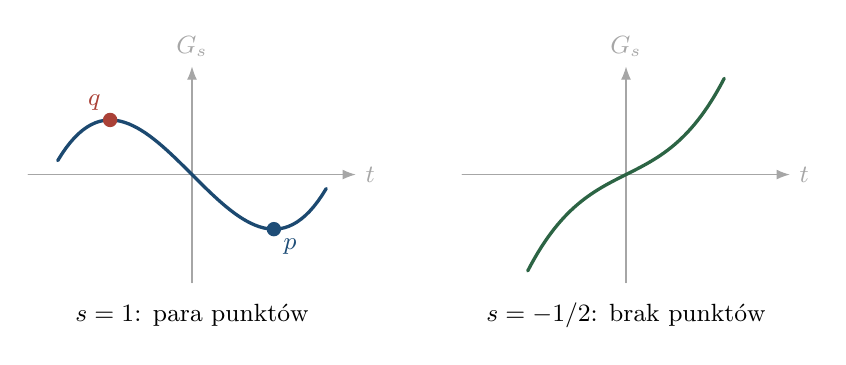
\begin{tikzpicture}[>=Latex,line cap=round,font=\small,scale=1.04]
 \draw[->,gray!70] (-2.0,0)--(2.0,0) node[right] {$t$};
 \draw[->,gray!70] (0,-1.32)--(0,1.32) node[above] {$G_s$};
 \draw[manifoldblue!80!black,very thick,
       domain=-1.64:1.64,samples=65]
      plot (\x,{\x*\x*\x/3-\x});
 \fill[manifoldred] (-1,{2/3}) circle (2.5pt)
       node[above left] {$q$};
 \fill[manifoldblue!85!black] (1,{-2/3}) circle (2.5pt)
       node[below right] {$p$};
 \node at (0,-1.72) {$s=1$: para punktów};
 \begin{scope}[shift={(5.3,0)}]
  \draw[->,gray!70] (-2.0,0)--(2.0,0) node[right] {$t$};
  \draw[->,gray!70] (0,-1.32)--(0,1.32) node[above] {$G_s$};
  \draw[manifoldgreen!80!black,very thick,
        domain=-1.20:1.20,samples=60]
       plot (\x,{\x*\x*\x/3+\x/2});
  \node at (0,-1.72) {$s=-1/2$: brak punktów};
 \end{scope}
\end{tikzpicture}
\caption{Przekrój modelu~\eqref{eq:narodziny-uchwytow-18}
przez oś $x=y=0$. Dla $s>0$ są dwa
punkty krytyczne o kolejnych indeksach
i jedna trajektoria od $q$ do $p$.
Po przejściu przez $s=0$ oba znikają.
Pozostałe kierunki $x,y$ ustalają indeksy.}
\label{fig:znoszenie-uchwytow-18}
\end{figure}

\begin{stwierdzenie}[Warunkowe przejście od przecięcia algebraicznego]
\label{prop:whitney-do-zniesienia-18}
Niech dla pary sąsiednich uchwytów
podpisana suma punktów $A_q\cap B_p$
wynosi $\pm1$. Jeśli punktów jest więcej niż jeden,
załóżmy, że można sparować wszystkie poza jednym
w pary o przeciwnych znakach i wybrać dla nich
rozłączne \emph{zanurzone, prawidłowo obramowane
dyski Whitneya}. Brzeg każdego dysku składa się
z łuku na $A_q$ i łuku na $B_p$, a jego wnętrze
omija wszystkie rozważane sfery. Wnętrza obu łuków
omijają pozostałe punkty $A_q\cap B_p$.
Wtedy po izotopii sfer
pozostaje jeden punkt przecięcia
i stosuje się
Twierdzenie~\ref{thm:zniesienie-18}.
\end{stwierdzenie}
\begin{proof}
Jeśli jest już jeden punkt, od razu stosujemy
twierdzenie o zniesieniu. W pozostałym przypadku
założenie o łukach wymaga dodatnich wymiarów obu sfer;
w szczególności $m\geq3$ i $1\leq k\leq m-2$,
gdzie indeksy uchwytów to $k,k+1$.
Wybierzmy jeden z założonych dysków.
„Prawidłowo obramowany” oznacza tutaj, że obramowanie
wzdłuż jego brzegu, wyznaczone przez kierunki
styczne i normalne obu sfer, przedłuża się na dysk.
Nie wystarcza sama trywialność jego wiązki normalnej:
ta dla dysku jest automatyczna, a warunek dotyczy
\emph{zadanego} obramowania brzegowego.
Rozpiszmy ruch w tym otoczeniu. Niech $r=k$ i $s=m-k-1$
będą wymiarami $A_q$ i $B_p$. Zgodne obramowanie i otoczenie
tubularne dają produktowy model
$U\times D^{r-1}\times D^{s-1}$, gdzie $U$ jest małym
otoczeniem płaskiego dysku o brzegu złożonym z dwóch łuków.
W tym modelu fragmenty sfer mają postać
\[
 A_q=\alpha\times D^{r-1}\times\{0\},\qquad
 B_p=\beta\times\{0\}\times D^{s-1}.
\]
Łuki $\alpha,\beta$ przedłużamy nieco poza ich dwa przecięcia.
Obramowanie uzgadnia kierunki styczne do sfer wzdłuż tych łuków
z kierunkami normalnymi do dysku; jego przedłużenie na dysk
pozwala pogrubić cały model, a nie tylko jego brzeg.
Jest to lokalny model z lematu~6.7 Milnora, tu przy założonym
istnieniu zanurzonego, czystego i prawidłowo obramowanego dysku.

W płaszczyźnie wybieramy izotopię $G_t$ przesuwającą $\alpha$
przez dysk na drugą stronę $\beta$, tak aby $G_1(\alpha)$
nie przecinała $\beta$. Jej nośnik mieści się we wnętrzu $U$.
Niech $\rho(u,v)$ będzie funkcją odcinającą równą $1$ blisko
$(0,0)$ i $0$ przy brzegu czynników normalnych. Wówczas
\[
 H_t(z,u,v)=\bigl(G_{t\rho(u,v)}(z),u,v\bigr)
\]
jest izotopią otoczenia, równą identyczności blisko jego brzegu:
dla ustalonych $u,v$ odwrotność daje $G_{t\rho(u,v)}^{-1}$.
Przecięcie $H_t(A_q)$ z nieruchomą $B_p$ wymaga $u=v=0$,
więc odpowiada dokładnie przecięciom $G_t(\alpha)$ z $\beta$.
Dla $t=1$ oba punkty znikają. Czystość dysku, warunek o wnętrzach
łuków i rozłączność dysków pozwalają wybrać otoczenie omijające
pozostałe punkty przecięcia i pozostałe dyski. Poza nim kładziemy
identyczność. Normalne pogrubienie przesuwanej sfery przenosimy
przez tę samą izotopię, zachowując dane przyczepienia uchwytu.
Powtarzamy ten ruch dla rozłącznych
dysków. Po każdym kroku liczba
punktów zmniejsza się o dwa, a
suma podpisana nie zmienia się.
Ponieważ na końcu wynosi $\pm1$,
pozostaje jeden punkt; poprzednie
twierdzenie usuwa parę uchwytów.
\end{proof}

\begin{uwaga}[Dlaczego potrzebny będzie wymiar]
Samo równanie $I(A_q,B_p)=\pm1$
nie zapewnia istnienia wymienionych
dysków. Trzeba znaleźć odpowiednie
łuki, wypełnić ich pętle, odsunąć
wnętrza dysków od sfer i sprawdzić
obramowanie. W wysokim wymiarze
pomagają prosta spójność i pozycja
ogólna; przy indeksach brzegowych
oraz w małych wymiarach występują
dodatkowe trudności. Szczegółowe
warunki triku Whitneya są zasadniczą
częścią dowodu twierdzenia Smale'a,
a nie konsekwencją samego rachunku
macierzy.
\end{uwaga}

\section{Granica tego rozdziału i dalszy krok}
\label{sec:uchwyty-smale-most-18}

Rozkład uchwytowy daje skończony
kompleks względny. Jeśli w kobordyzmie
obie inkluzje końców są równoważnościami
homotopijnymi, mówimy o
\emph{$h$-kobordyzmie}. Wtedy
$H_*(W,N_-)=0$, więc kompleks
uchwytów jest acykliczny.
Rachunek macierzy sugeruje pary
uchwytów do zniesienia, lecz
aby naprawdę uzyskać iloczyn
$N_-\times[0,1]$, trzeba
zrealizować operacje algebraiczne
przez przesunięcia i usunąć
zbędne przecięcia trikiem Whitneya.
W przypadku prostej spójności i
wymiaru $m\geq6$ prowadzi to do
twierdzenia Smale'a o $h$-kobordyzmie.
Bez prostej spójności pojawia się
dodatkowa przeszkoda, torsja
Whiteheada; jej analiza należy
do twierdzenia o $s$-kobordyzmie.
Nie jest to inwariant samego powyższego kompleksu nad $\Z$.
Dla spójnego $W$ i grupy $\pi=\pi_1(W)$ trzeba podnieść uchwyty
do nakrycia uniwersalnego i pracować nad pierścieniem
grupowym $\Z[\pi]$. Współczynniki zapamiętują wtedy
także klasy dróg, a nie tylko sumy znaków przecięć.
Acykliczność zwykłego kompleksu całkowitego
nie wystarcza do rozpoznania tej przeszkody.

Drugi kierunek to teoria chirurgii:
Twierdzenie~\ref{thm:slad-chirurgii-18}
tłumaczy każdy uchwyt na operację
na poziomicy, a obramowanie mówi,
jak wykonać sklejanie. Naturalnym dalszym krokiem byłoby zbadanie, jakie
inwarianty homologiczne i formy
przecięcia można zmienić przez
dobór takich operacji.
Nie zakładamy tu, że wszystkie
przeszkody można usunąć;
zwłaszcza przypadki małych
wymiarów wymagają osobnej analizy.

\par\smallskip
{\footnotesize\noindent\emph{Dalsza lektura:}
\href{https://www.cambridge.org/core/books/differential-topology/theory-of-handle-decompositions/BA54EF1BD9B755DFA2B363176B0CA2F7}{C.\,T.\,C.\ Wall, \emph{Differential Topology}, rozdział o rozkładach uchwytowych},
\href{https://webhomes.maths.ed.ac.uk/~v1ranick/books/surgery.pdf}{A.\ Ranicki, \emph{Algebraic and Geometric Surgery}, ślad chirurgii i kompleks uchwytowy},
\href{https://www.math.columbia.edu/~jmorgan/Lecture_IIIA_hcobordism_Contd.pdf}{J.\ Morgan, wykład o znoszeniu uchwytów i triku Whitneya},
\href{https://webhomes.maths.ed.ac.uk/~v1ranick/surgery/hcobord.pdf}{J.\ Milnor, \emph{Lectures on the h-Cobordism Theorem}, \S6, zwłaszcza lemat~6.7 i ruch w jego produktowym modelu}.\par}

\chapter{Twierdzenie Smale'a o \texorpdfstring{$h$}{h}-kobordyzmie}
\label{ch:hcobordyzm}
\index{h-kobordyzm@$h$-kobordyzm}

W poprzednim rozdziale nauczyliśmy się
przesuwać uchwyty i znosić parę, której
sfery spotykają się w jednym punkcie.
Teraz zastosujemy te ruchy do całego
kobordyzmu. Intuicja jest prosta:
jeśli oba brzegi $W$ zachowują w nim
całą informację homotopijną, wszystkie
uchwyty powinny występować w parach,
które nie wnoszą trwałej topologii.
Dowód musi jeszcze zamienić to zdanie
o \emph{homotopii} na stwierdzenie
o \emph{dyfeomorfizmie}.

Przez cały rozdział $(W;N_-,N_+)$
oznacza zwarty, spójny, gładki
kobordyzm wymiaru $m$ z dwoma
niepustymi spójnymi brzegami.
Używamy oznaczeń rdzenia, sfery
przyczepienia $A$ i sfery pasa $B$
z Rozdziału~\ref{ch:rachunek-uchwytow}.
Liczby przecięcia dotyczą poziomicy
wymiaru $m-1$.

\section{Co dokładnie orzeka twierdzenie?}
\label{sec:stwierdzenie-hc-19}

\begin{twierdzenie}[Smale, twierdzenie o $h$-kobordyzmie]
\label{thm:smale-hc-19}
Załóżmy, że $m\geq6$, rozmaitość
$W^m$ jest po prostu spójna, a obie
inkluzje $N_\pm\hookrightarrow W$
są równoważnościami homotopijnymi.
Wówczas istnieje dyfeomorfizm
\[
 \Phi:N_-\times[0,1]\longrightarrow W,
 \qquad \Phi(x,0)=x.
\]
W szczególności $N_-\cong N_+$
jako rozmaitości gładkie.
\end{twierdzenie}

To twierdzenie dotyczy \emph{gładkiej}
struktury $W$; końcowy dyfeomorfizm
na $N_+$ nie jest z góry wybrany.
Termin \emph{$h$-kobordyzm} dla
warunku o obu inkluzjach pojawił się
w Sekcji~\ref{sec:uchwyty-smale-most-18}.
Prosta spójność $W$ wraz z tymi
równoważnościami oznacza też
$\pi_1(N_-)=\pi_1(N_+)=0$.

\begin{stwierdzenie}[Acykliczność]
\label{prop:acykliczny-hc-19}
W warunkach
Twierdzenia~\ref{thm:smale-hc-19}
zachodzi
\[
 H_j(W,N_-;\Z)=0
 \qquad\text{dla każdego }j.
\]
Kompleks uchwytów z
Twierdzenia~\ref{thm:kompleks-uchwytow-18}
jest zatem acykliczny.
\end{stwierdzenie}
\begin{proof}
Równoważność homotopijna
$N_-\hookrightarrow W$ indukuje
izomorfizm wszystkich grup homologii.
W długim ciągu dokładnym pary
\[
 \cdots\to H_j(N_-)\to H_j(W)
 \to H_j(W,N_-)\to H_{j-1}(N_-)
 \to H_{j-1}(W)\to\cdots
\]
oba widoczne odwzorowania indukowane inkluzją
są izomorfizmami. Dokładność wymusza
zatem zerowanie grupy pośrodku.
Kompleks uchwytów oblicza te grupy,
więc jego homologia jest zerowa.
\end{proof}

Acykliczność mówi, że macierze
$\partial_k$ zawierają informację
o możliwych \emph{algebraicznych}
parach. Nie mówi jeszcze, czy
sfery spotykają się tylko raz.
Rysunek~\ref{fig:plan-smale-19}
pokazuje drogę od tego faktu
do iloczynu.

\begin{figure}[htbp]
\centering
\begin{tikzpicture}[>=Latex,font=\small,
 every node/.style={align=center,rounded corners=3pt,
                    inner sep=5pt}]
 \node[draw=manifoldblue!70!black,fill=manifoldblue!9]
      (a) at (-2.55,.90) {acykliczny kompleks\\uchwytów};
 \node[draw=manifoldgold!85!black,fill=manifoldgold!12]
      (b) at (2.55,.90) {przesunięcia\\macierz z blokami $1$};
 \node[draw=manifoldgreen!70!black,fill=manifoldgreen!10]
      (c) at (2.55,-.90) {trik Whitneya\\jeden punkt na parę};
 \node[draw=manifoldred!75!black,fill=manifoldred!7]
      (d) at (-2.55,-.90) {znoszenie uchwytów\\$W\cong N_-\times[0,1]$};
 \draw[->,thick] (a)--(b);
 \draw[->,thick] (b)--(c);
 \draw[->,thick] (c)--(d);
\end{tikzpicture}
\caption{Cztery etapy dowodu. Acykliczność
jest algebraiczna; między nią a zniesieniem
uchwytów potrzebne są ruchy geometryczne.}
\label{fig:plan-smale-19}
\end{figure}

\begin{lemat}[Brak punktów krytycznych oznacza iloczyn]
\label{lem:brak-krytycznych-hc-19}
Jeżeli funkcja Morse'a $F:W\to[0,1]$,
stała na odpowiednich brzegach,
nie ma punktów krytycznych, to
$W\cong N_-\times[0,1]$
względem $N_-$.
\end{lemat}
\begin{proof}
Wybierzmy metrykę Riemanna i pole
$X=\nabla F/|\nabla F|^2$.
Mianownik jest dodatni na całym
zwartym $W$, więc $X$ jest gładkie.
Wzdłuż jego trajektorii
$\frac{\dd}{\dd t}F(\varphi_t(x))
 =\dd F(X)=1$.
Trajektoria wychodząca z $x\in N_-$
dochodzi do poziomu $t$ po czasie $t$.
Nie urywa się wcześniej: między
poziomami leży w zwartym $W$,
a w kołnierzach pole jest poprzeczne
do brzegu. Odwrócenie czasu
przenosi każdy punkt $W$
jednoznacznie na $N_-$.
Odwzorowanie $(x,t)\mapsto\varphi_t(x)$
jest więc bijekcją, jest gładka,
a jej odwrotność
$y\mapsto(\varphi_{-F(y)}(y),F(y))$
też jest gładka.
\end{proof}

\section{Usunięcie indeksów skrajnych}
\label{sec:skrajne-hc-19}

Najpierw usuwamy uchwyty indeksów
$0,m$, potem zastępujemy indeksy
$1,m-1$ uchwytami o indeksach
bardziej środkowych. Ta druga
operacja nazywa się czasem
\emph{wymianą uchwytu}
(ang.\ \emph{handle trading}):
liczba punktów krytycznych
nie musi w tym kroku maleć.

\begin{lemat}[Znoszenie $0$- i $m$-uchwytów]
\label{lem:zero-m-hc-19}
Jeżeli oba brzegi i $W$ są spójne,
to funkcję Morse'a zgodną z brzegiem
można zmienić we wnętrzu tak, aby
nie miała punktów krytycznych
indeksu $0$ ani $m$.
\end{lemat}
\begin{proof}
Uporządkujmy uchwyty według indeksów
(Twierdzenie~\ref{thm:przestawianie-18}).
Tuż po wszystkich $1$-uchwytach
części utworzone z $N_-\times[0,1]$
i z $0$-uchwytów są wierzchołkami
grafu: każdy $1$-uchwyt jest krawędzią
łączącą dwie części albo pętlą.
Uchwyty indeksu co najmniej $2$
nie łączą różnych składowych
(ich sfery przyczepienia są spójne),
więc spójność $W$ oznacza,
że ten graf jest spójny.

Wybieramy w nim drzewo rozpinające
z korzeniem odpowiadającym $N_-$.
Dla wierzchołka reprezentującego
$0$-uchwyt wybieramy krawędź drzewa,
która łączy go w kierunku korzenia.
W pośrednim brzegu odpowiadającym
temu etapowi jedna stopa
$1$-uchwytu leży na sferze pasa
wybranego $0$-uchwytu, a druga
na innej składowej brzegu.
Sfera przyczepienia $S^0$
spotyka więc tę sferę pasa
\emph{w dokładnie jednym punkcie}.
Możemy rozdzielić wartości
krytyczne od wartości innych
uchwytów indeksu $0$ i $1$
i zastosować
Twierdzenie~\ref{thm:zniesienie-18}.
Pozostałe uchwyty są przenoszone
przez powstały pas iloczynowy.
Powtarzamy procedurę dla
wszystkich $0$-uchwytów.

W odwróconym kobordyzmie
funkcja $1-F$ zamienia indeks $m$
na $0$ oraz $m-1$ na $1$,
zgodnie z
Twierdzeniem~\ref{thm:dualny-uchwyt-18}.
Ten sam argument przy spójnym
$N_+$ usuwa wszystkie $m$-uchwyty.
\end{proof}

Sam brak indeksów $0,m$
nie wystarcza: $1$-uchwyty
zmieniają $\pi_1$ poziomic,
a dysk Whitneya dla sfer
z nimi związanych może mieć
niewłaściwy wymiar. Poniższy
krok wyjaśnia rolę prostej
spójności.

\begin{lemat}[Wymiana indeksu $1$ na $3$]
\label{lem:handel-trade-hc-19}
Jeśli $m\geq6$, $N_-$ i $W$ są
po prostu spójne, a w rozkładzie
nie ma $0$-uchwytów, to można
usunąć wszystkie $1$-uchwyty,
dopuszczając w zamian nowe
$3$-uchwyty. W odwróconym
kobordyzmie analogicznie
usuwa się indeks $m-1$
na rzecz $m-3$.
\end{lemat}
\begin{proof}
Weźmy jeden $1$-uchwyt $q$.
Po jego dołączeniu w poziomicy
jest sfera pasa $B_q\cong S^{m-2}$.
Poziomica po wszystkich $1$-uchwytach składa się z $N_-$
z usuniętymi wnętrzami rozłącznych kul, odpowiadających stopom,
oraz z rurek $D^1\times S^{m-2}$.
Pozostałość $N_-$ jest spójna: drogę przecinającą usuniętą kulę
można zastąpić drogą po jej spójnym brzegu.
Łączymy więc dwie stopy $q$ zanurzonym łukiem w tej pozostałości
i zamykamy go łukiem $D^1\times\{z\}$ w rurce $q$.
Po wygładzeniu otrzymujemy zanurzony okrąg
$\gamma$ przecinający $B_q$
raz i omijający sfery pasa
pozostałych $1$-uchwytów.
Ominięcie pozostałych sfer pasa wynika z tego, że nie wchodzimy
do pozostałych rurek, nie z samej transwersalności: te sfery mają
w poziomicy kowymiar $1$.

Możemy przeprowadzić $\gamma$
w górę przez poziom starych
$2$-uchwytów: okrąg i ich
sfery przyczepienia są
jednowymiarowe, więc przy
$m-1\geq5$ pozycja ogólna
pozwala je rozsunąć.
Otrzymany okrąg $\gamma'$ leży w poziomicy $L_2$ po wszystkich
starych $2$-uchwytach. Jego dostatecznie małe otoczenie także
przepływa przez ten pas i omija sfery pasa starych $2$-uchwytów.
Ta poziomica jest po prostu
spójna. Istotnie, jej dolna
podpoziomica ma to samo $\pi_1$
co $W$, gdyż późniejsze uchwyty
mają indeksy co najmniej $3$.
Oglądając dolną podpoziomicę
od góry, przyczepiamy do
rozważanej poziomicy jedynie
uchwyty dualne indeksu
co najmniej $m-2\geq4$,
które także nie zmieniają
$\pi_1$. Zatem $\gamma'$ ogranicza w $L_2$ odwzorowanie dysku.
Wybieramy jego gładki kołnierz przy zadanym zanurzonym brzegu.
Względna pozycja ogólna pozwala poprawić wnętrze do zanurzenia
$d:D^2\hookrightarrow L_2$: dla samoprzecięć mamy
$2+2-(m-1)<0$, a zbiór punktów utraty rzędu różniczki ma
oczekiwany kowymiar $m-2>2$ w dziedzinie.

Teraz wybieramy mały okrąg $C=d(\varepsilon S^1)$ we wnętrzu
tego dysku. Rodzina $z\mapsto d(rz)$ dla $z\in S^1$ i
$\varepsilon\leq r\leq1$ jest \emph{izotopią} od $C$ do
$\gamma'$: każdy jej przekrój jest zanurzonym okręgiem.
To sprawdzenie przekrojów jest istotne; samo zanurzenie cylindra
opisującego homotopię nie dawałoby takiego wniosku.

W małym regularnym pasie nad okolicą $d(0)$ tworzymy
\emph{nową} parę punktów krytycznych indeksów $2,3$ według
modelu~\eqref{eq:narodziny-uchwytow-18} przy $k=2$.
Dobieramy lokalne współrzędne tak, by sferą przyczepienia nowego
$2$-uchwytu był $C$, ze standardowym obramowaniem tego modelu.
Nie nadajemy urodzonemu uchwytowi dowolnie skręconego obramowania.
Przenosimy jego obramowanie razem z izotopią $C\to\gamma'$.
Twierdzenie o przedłużaniu izotopii
(Sekcja~\ref{sec:izotopie-otoczen-15}) przedłuża ten ruch na
otoczenie, a zmiana pola gradientopodobnego w regularnym pasie
realizuje nowe przyklejenie. Końcowe pogrubienie można zmieścić
w dowolnie małym otoczeniu $\gamma'$; po jego zwężeniu
całe obramowane przyklejenie przepływa więc w dół do $\gamma$.

Wyjaśnijmy przestawienie wartości krytycznych. Nowy $2$-uchwyt
nie ma trajektorii spadku do żadnego starego $2$-uchwytu:
jego sfera przyczepienia omija ich sfery pasa, ponieważ pochodzi
z przepływu $\gamma$ przez regularne trajektorie.
Twierdzenie~\ref{thm:przestawianie-18} pozwala zatem kolejno
przenieść go poniżej wszystkich starych $2$-uchwytów.
Wybrany $1$-uchwyt $q$ ustawiamy jako ostatni w bloku
$1$-uchwytów. Nowy $2$-uchwyt następuje bezpośrednio po nim,
a $\gamma$ spotyka jego sferę pasa poprzecznie dokładnie raz.
Twierdzenie~\ref{thm:zniesienie-18}
usuwa zatem dawny
$1$-uchwyt i nowy
$2$-uchwyt. Nowy
$3$-uchwyt zostaje.

Wykonujemy ten ruch osobno
dla kolejnych $1$-uchwytów.
Po odwróceniu całego
kobordyzmu indeksy
$1,2,3$ stają się
$m-1,m-2,m-3$;
tym samym argumentem
usuwamy $m-1$-uchwyty. Ponieważ $m-3\geq3$, nie odtwarzamy
przy tym usuniętych wcześniej indeksów $0$ ani $1$.
\end{proof}

\begin{figure}[htbp]
\centering
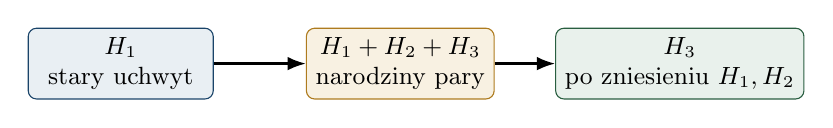
\begin{tikzpicture}[>=Latex,font=\small,
 every node/.style={align=center}]
 \node[draw=manifoldblue!75!black,fill=manifoldblue!10,
       rounded corners=3pt,minimum width=2.35cm,
       minimum height=.85cm] (a) at (-3.55,0)
       {$H_1$\\stary uchwyt};
 \node[draw=manifoldgold!85!black,fill=manifoldgold!13,
       rounded corners=3pt,minimum width=2.35cm,
       minimum height=.85cm] (b) at (0,0)
       {$H_1+H_2+H_3$\\narodziny pary};
 \node[draw=manifoldgreen!75!black,fill=manifoldgreen!11,
       rounded corners=3pt,minimum width=2.35cm,
       minimum height=.85cm] (c) at (3.55,0)
       {$H_3$\\po zniesieniu $H_1,H_2$};
 \draw[->,thick] (a)--(b);
 \draw[->,thick] (b)--(c);
\end{tikzpicture}
\caption{Wymiana $1$-uchwytu na $3$-uchwyt.
Para $H_2,H_3$ powstaje lokalnie; następnie
przesuwamy sferę przyczepienia $H_2$
i znosimy $H_1$ z $H_2$.}
\label{fig:wymiana-1-na-3-19}
\end{figure}

\begin{uwaga}[Co zostało użyte?]
\label{uwaga:wymiana-warunki-19}
Prosta spójność poziomicy służy
do przesunięcia okręgu
$\gamma'$ na $C$; bez niej
nie można uzasadnić tego kroku
samą homologią. Wymiar
co najmniej $5$ poziomicy
pozwala zbudować zanurzony dysk, którego koncentryczne okręgi
dają potrzebną izotopię. Kwestia normalnego obramowania
jest tu częścią standardowego modelu lokalnie tworzonej pary
i transportu jego danych przez izotopię;
to dodatkowa dana geometryczna,
której nie pokazuje schemat.
\end{uwaga}

\section{Trik Whitneya: od liczby do jednego punktu}
\label{sec:whitney-hc-19}

Po Lemacie~\ref{lem:handel-trade-hc-19}
indeksy wszystkich uchwytów leżą
między $2$ a $m-2$.
Niech $k$ będzie najmniejszym
występującym indeksem.
Ponieważ kompleks względny jest
acykliczny, jeśli pozostały uchwyty,
to $k\leq m-3$: gdyby występowały
jedynie uchwyty indeksu $m-2$,
ich wolne generatory dawałyby
niezerowe $H_{m-2}(W,N_-)$.

Ustalmy poziomicę $L$ między
uchwytami indeksów $k$ i $k+1$.
Sfery pasa $k$-uchwytów
oznaczamy $B_1,\ldots,B_r$,
a sfery przyczepienia
$(k+1)$-uchwytów
$A_1,\ldots,A_s$.
Mają w $L^{m-1}$ wymiary
\[
 \dim A_j=k,\qquad
 \dim B_i=m-k-1,\qquad
 \dim A_j+\dim B_i=m-1.
\]
Po transwersalnej perturbacji
przecinają się w skończenie
wielu punktach. Współczynnik
macierzy $\partial_{k+1}$
jest \emph{sumą ich znaków},
jak w~\eqref{eq:macierz-uchwyty-18}.

\begin{lemat}[Prosta spójność poziomicy i jej dopełnienia]
\label{lem:komplement-whitney-19}
W sytuacji z poprzedniego akapitu
załóżmy, że $N_-$ i $N_+$ są
po prostu spójne, $2\leq k\leq m-3$, a wszystkie uchwyty
mają indeksy od $k$ do $m-2$. Poziomica $L$ leży po wszystkich
$k$-uchwytach i przed wszystkimi $(k+1)$-uchwytami.
Wtedy $L$ oraz dopełnienie
\[
 L\setminus
   \left(\bigcup_i B_i\ \cup\ \bigcup_j A_j\right)
\]
są po prostu spójne.
\end{lemat}
\begin{proof}
Oznaczmy przez $W_-$ część
kobordyzmu od $N_-$ do $L$.
Ponieważ przed $L$ przyczepiano
tylko uchwyty indeksu $k$,
a $k\geq2$, te uchwyty nie mogą
\emph{utworzyć} nowej grupy
fundamentalnej ze spójnego,
po prostu spójnego $N_-$:
$2$-komórka może zabić pętlę,
a komórki wyższego wymiaru
nie zmieniają $\pi_1$.
Stąd $\pi_1(W_-)=0$.
Odwróćmy fragment $W_-$.
Jest zbudowany z $L$
przez dołączanie uchwytów
dualnych indeksu $m-k\geq3$.
One nie zmieniają $\pi_1$,
zatem $\pi_1(L)=0$.

Jeżeli $2<k<m-3$, to
$\operatorname{codim}_L B_i=k\geq3$
i $\operatorname{codim}_L A_j
=m-k-1\geq3$.
Usuwanie skończonej sumy
takich podrozmaitości nie
zmienia $\pi_1$.
Aby to zobaczyć, przesuwamy
pętlę na mocy transwersalności
poza te zbiory.
Jej homotopia wypełniająca
ma wymiar $2$ i również
może ich uniknąć, ponieważ
$2+\dim B_i<\dim L$
i $2+\dim A_j<\dim L$.
Dlatego dopełnienie jest
po prostu spójne.

Trzeba osobno sprawdzić
$k=2$, gdy $B_i$ ma
kowymiar $2$ w $L$.
Usuwamy najpierw wszystkie $B_i$.
Niech $E$ będzie $N_-$ z usuniętymi wnętrzami rozłącznych
otoczeń przyczepienia $S^1\times D^{m-2}$.
W $L\setminus\bigcup B_i$ do $E$ doklejono kawałki
$(D^2\setminus\{0\})\times S^{m-3}$.
Radialna retrakcja $D^2\setminus\{0\}$ na $S^1$, stała
na tym brzegu, daje retrakcję deformacyjną całej przestrzeni na $E$.
Z drugiej strony $N_-$ z usuniętymi samymi okręgami przyczepienia
powstaje przez doklejenie do $E$ kawałków
$S^1\times(D^{m-2}\setminus\{0\})$; one też retrahują się
radialnie na wspólny brzeg $S^1\times S^{m-3}$.
Obie przestrzenie mają zatem ten sam typ homotopijny co $E$,
co uzasadnia porównanie ich grup fundamentalnych.
W $N_-^{m-1}$ mają one
kowymiar $m-2\geq4$;
z poprzedniego argumentu
ich usunięcie nie zmienia
$\pi_1(N_-)=0$.
Następnie usuwamy $A_j$,
których kowymiar wynosi
$m-3\geq3$, więc $\pi_1$
pozostaje zerowa.
Dla $k=m-3$ nad $L$ są już tylko uchwyty indeksu $m-2$.
Po odwróceniu \emph{górnego fragmentu} od $N_+$ do $L$
są one $2$-uchwytami, a ich sferami pasa są obecne $A_j$.
Ten sam argument daje $\pi_1(L\setminus\bigcup A_j)=0$.
Następnie usuwamy $B_i$, mające kowymiar $m-3\geq3$.
Nie zakładamy więc ogólnej prostej spójności dopełnienia sfer
kowymiaru $2$; wynika ona z konkretnego rozkładu uchwytowego.
Spójność drogowa wszystkich użytych dopełnień wynika z tego samego
opisu i z przesuwania dróg poza podrozmaitości kowymiaru co najmniej $2$.
\end{proof}

\begin{lemat}[Trik Whitneya dla rozważanych sfer]
\label{lem:whitney-hc-19}
W warunkach
Lematu~\ref{lem:komplement-whitney-19}
niech $A_j$ i $B_i$
przecinają się w dwóch
punktach $u,v$ o przeciwnych
znakach. Można zmienić
pole gradientopodobne
w małym pasie wokół $L$,
tak aby te dwa punkty
zniknęły, bez zmiany innych
punktów przecięcia
którejkolwiek pary sfer.
\end{lemat}
\begin{proof}
\emph{Krok 1: brzeg dysku.}
Wybieramy łuk $\alpha\subset A_j$
od $u$ do $v$ i łuk
$\beta\subset B_i$ w przeciwnym
kierunku. Ich wnętrza
omijają pozostałe punkty
przecięcia: obie sfery mają
wymiar co najmniej $2$,
a usuwamy zeń tylko
skończony zbiór.
Suma $\alpha\cup\beta$
jest zamkniętą krzywą
o dwóch narożach.
W małym otoczeniu tej krzywej
odsuwamy jej równoległą
kopię od obu rodzin sfer.
Ta kopia leży w dopełnieniu
z poprzedniego lematu,
więc jest tam homotopijnie
trywialna.

\emph{Krok 2: wypełnienie.}
Wybierzmy odwzorowanie dysku
rozpinające odsuniętą pętlę
w tym dopełnieniu.
Transwersalność względna
pozwala uczynić je
zanurzeniem, bo oczekiwany
wymiar samoprzecięć
dwóch fragmentów
dwuwymiarowego dysku
wynosi $2+2-(m-1)<0$.
Dołączając wąski kołnierz
od równoległej kopii do
$\alpha\cup\beta$
i zachowując standardowe naroża w $u,v$,
otrzymujemy zanurzony
dysk $D$ o brzegu leżącym
na $A_j\cup B_i$,
którego wnętrze omija
\emph{wszystkie} $A$ i $B$.
Jest to dysk Whitneya.

\emph{Krok 3: obramowanie.}
Samo zanurzenie dysku $D$ nie
wystarcza do wykonania ruchu.
Wzdłuż $\alpha$ i $\beta$ obie sfery
wyznaczają kierunki, w których
należy przesunąć ich pasy. Potrzebne
jest przedłużenie tych danych do
\emph{obramowanego dysku Whitneya}.
Zgodność znaków na końcach łuków
jest konieczna, lecz sama nie
dowodzi istnienia takiego przedłużenia:
trzeba także skontrolować skręcenie
normalne wzdłuż całego brzegu.
Używamy następującego \emph{wyniku zewnętrznego}.
Niech $P^r,Q^s$ będą domkniętymi, poprzecznie przecinającymi się
gładkimi podrozmaitościami $V^{r+s}$ bez brzegu. Orientujemy $P$
i wiązkę normalną $Q$. Załóżmy $r\geq2$, $s\geq3$, $r+s\geq5$.
Dla $r=2$ wymagamy dodatkowo injektywności
$\pi_1(V\setminus Q)\to\pi_1(V)$.
Jeśli punkty $u,v$ mają przeciwne znaki i łączą je łuki w $P,Q$
o wnętrzach omijających pozostałe przecięcia, a ich suma jest
ściągalna w $V$, istnieje izotopia otoczenia $h_t$, zaczynająca się
od identyczności, taka że
\[
 h_1(P)\cap Q=(P\cap Q)\setminus\{u,v\}.
\]
Izotopia jest identyczna blisko pozostałych przecięć.
Porównujemy tu poruszony zbiór $h_1(P)$ ze stałym zbiorem $Q$;
nie twierdzimy, że $h_t$ unieruchamia punktowo całe $Q$.
Konstrukcja daje produktowe otoczenie odpowiednio
dobranego dysku Whitneya, zgodne z obiema podrozmaitościami.
Dokładny wynik i konstrukcja obramowania znajdują się w
\href{https://webhomes.maths.ed.ac.uk/~v1ranick/surgery/hcobord.pdf}
{J.\ Milnor, \emph{Lectures on the $h$-Cobordism Theorem},
twierdzenie 6.6 oraz lematy 6.7 i 6.13}.
Nie zastępujemy tego lematu stwierdzeniem, że każda wiązka nad
dyskiem jest trywialna: trzeba przedłużyć \emph{zadane dane brzegowe}.

Sprawdźmy hipotezy dla całych rodzin sfer. Gdy $k\leq m-4$,
bierzemy $P=\bigcup A_j$, $Q=\bigcup B_i$,
$r=k$, $s=m-k-1\geq3$. Dla $k=2$ dowód poprzedniego lematu
daje już $\pi_1(L\setminus\bigcup B_i)=0$; dla $k>2$
dodatkowy warunek nie jest potrzebny. Gdy $k=m-3$,
zamieniamy role: $P=\bigcup B_i$, $Q=\bigcup A_j$,
$r=2$, $s=m-3\geq3$; dualny argument daje
$\pi_1(L\setminus\bigcup A_j)=0$.
Orientacje bierzemy z orientacji sfer i ich obramowań uchwytowych.
Pętla jest ściągalna, bo $L$ jest po prostu spójna.
Zastosowanie do całych rodzin chroni także przecięcia z pozostałymi
sferami. W drugim przypadku wynik początkowo porusza rodzinę $B$;
odwrotna izotopia porusza rodzinę $A$ względem nieruchomego $B$
i usuwa tę samą parę.

W obu przypadkach otrzymujemy obramowane
otoczenie
\[
 D^2\times D^{k-1}
       \times D^{m-k-2}
\]
o wymiarze $m-1$,
w którym $A_j$ i $B_i$
są dwiema standardowymi
poprzecznymi rodzinami pasów.

\emph{Krok 4: ruch.}
W tym otoczeniu przesuwamy
pas $A_j$ przez $D^2$,
pozostawiając go nieruchomo poza tym otoczeniem oraz przy końcach łuku
przedłużonego \emph{poza} $u,v$. Samych punktów $u,v$ nie
unieruchamiamy: muszą opuścić drugą sferę. W płaskim
przekroju wygląda to jak
usunięcie dwóch przecięć
z Rysunku~\ref{fig:whitney-hc-19}.
Iloczynowa postać normalnych
kierunków zapewnia,
że ten sam ruch jest izotopią
w pełnym wymiarze $m-1$.
Ponieważ wnętrze dysku
nie spotyka pozostałych sfer,
nie powstają dodatkowe
punkty przecięcia.
Przedłużamy izotopię
na regularny pas przepływu
i modyfikujemy tam pole
gradientopodobne; funkcja
i jej punkty krytyczne
pozostają bez zmian.
\end{proof}

\begin{figure}[htbp]
\centering
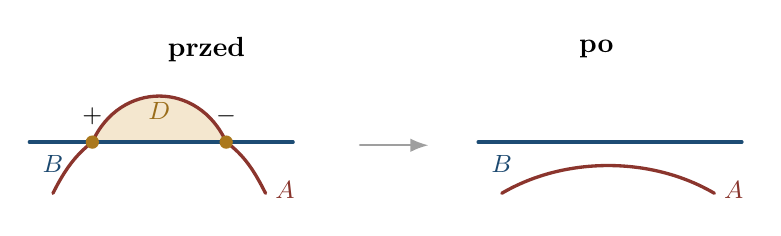
\begin{tikzpicture}[>=Latex,font=\small,line cap=round,scale=1.0]
 \node[font=\bfseries] at (-2.4,1.18) {przed};
 \node[font=\bfseries] at (2.55,1.18) {po};
 \begin{scope}[shift={(-4.7,0)}]
  \fill[manifoldgold!22]
    (.85,0) .. controls (1.20,.78) and (2.20,.78)
       .. (2.55,0) -- cycle;
  \draw[manifoldblue!83!black,very thick]
    (.05,0)--(3.40,0);
  \draw[manifoldred!82!black,very thick]
    (.35,-.65) .. controls (.50,-.35) and (.64,-.16)
     .. (.85,0) .. controls (1.20,.78) and (2.20,.78)
     .. (2.55,0) .. controls (2.77,-.16)
         and (2.90,-.35) .. (3.05,-.65);
  \fill[manifoldgold!83!black] (.85,0) circle (2.4pt);
  \fill[manifoldgold!83!black] (2.55,0) circle (2.4pt);
  \node[anchor=south] at (.85,.10) {$+$};
  \node[anchor=south] at (2.55,.10) {$-$};
  \node[manifoldgold!75!black] at (1.70,.40) {$D$};
  \node[manifoldblue!80!black,anchor=north] at (.35,-.04) {$B$};
  \node[manifoldred!80!black,anchor=west] at (3.05,-.61) {$A$};
 \end{scope}
 \draw[->,gray!75,thick] (-.45,-.04)--(.42,-.04);
 \begin{scope}[shift={(1.0,0)}]
  \draw[manifoldblue!83!black,very thick]
    (.05,0)--(3.40,0);
  \draw[manifoldred!82!black,very thick]
    (.35,-.65) .. controls (1.15,-.18)
           and (2.25,-.18) .. (3.05,-.65);
  \node[manifoldblue!80!black,anchor=north] at (.35,-.04) {$B$};
  \node[manifoldred!80!black,anchor=west] at (3.05,-.61) {$A$};
 \end{scope}
\end{tikzpicture}
\caption{Dwuwymiarowy przekrój triku Whitneya:
punkty o przeciwnych znakach są końcami
brzegu złotego dysku $D$. Przesunięcie
czerwonej sfery usuwa oba punkty.
Sam dowód działa w poziomicy
wymiaru co najmniej $5$;
rysunek nie przedstawia jej
pozostałych wymiarów.}
\label{fig:whitney-hc-19}
\end{figure}

\begin{przyklad}[Dlaczego $\pm1$ to za mało bez triku?]
Niech para sfer ma trzy punkty
przecięcia o znakach $+,+,-$.
Ich liczba algebraiczna to $1$,
lecz geometryczna liczba wynosi $3$.
Trik usuwa parę $+,-$ i pozostawia
jeden punkt $+$. Dopiero teraz
Twierdzenie~\ref{thm:zniesienie-18}
pozwala znieść uchwyty.
\end{przyklad}

\begin{uwaga}[Znaczenie założeń wymiarowych]
Dla wymiaru poziomicy $4$
wypełniający dysk może sam siebie
przecinać, ponieważ $2+2-4=0$.
Dlatego argument z Kroku 2
nie dowodzi twierdzenia o
gładkich $5$-wymiarowych
$h$-kobordyzmach.
Nie zakładamy też, że
zerowa liczba przecięcia
zawsze daje dysk Whitneya:
potrzebna była prosta
spójność \emph{dopełnienia}
całej rodziny sfer.
\end{uwaga}

\section{Od macierzy do geometrycznych par}
\label{sec:macierze-hc-19}

Po zniesieniu indeksów skrajnych
najmniejszy indeks oznaczmy $k$.
Brak $C_{k-1}$ oraz
$H_k(C_\bullet)=0$ dają
$\operatorname{im}\partial_{k+1}
=\ker\partial_k=C_k$.
Macierz
\[
 \partial_{k+1}:\Z^s\longrightarrow\Z^r,
 \qquad r=\#\{k\text{-uchwytów}\},
\]
jest więc \emph{surjektywna}.
Nad $\Z$ wolno wykonywać
wyłącznie operacje z
całkowitymi współczynnikami;
dzielenie przez liczbę $2$
zmieniłoby problem geometryczny.

\begin{lemat}[Całkowita redukcja przez kolumny]
\label{lem:macierz-surj-hc-19}
Niech $A:\Z^s\to\Z^r$
będzie surjekcją.
Permutacje kolumn, zmiana
znaku kolumny i dodawanie
całkowitej wielokrotności
jednej kolumny do drugiej
przeprowadzają jej macierz
do postaci
\[
       \begin{pmatrix}I_r&0\end{pmatrix}.
\]
Nie trzeba zmieniać
wybranej bazy $\Z^r$.
\end{lemat}
\begin{proof}
Dowodzimy przez indukcję po $r$.
Dla $r=0$ nie ma czego robić.
Pierwszy wiersz macierzy
surjektywnej ma wpisy
o największym wspólnym
dzielniku $1$: pierwszy
współrzędny obraz całej
$\Z^s$ jest równy $\Z$.
Algorytm Euklidesa można
wykonać operacjami na
\emph{kolumnach}.
Jeśli w dwóch miejscach
pierwszego wiersza stoją
$a,b$ z $b\ne0$, dzielimy
$a=qb+t$, $|t|<|b|$,
i zastępujemy odpowiednią
kolumnę przez nią minus
$q$ razy drugą. Powtarzając
otrzymujemy wpis $\pm1$.
Permutujemy go do pierwszej
kolumny i zmieniamy znak,
aby uzyskać $1$.
Odejmując wielokrotności
pierwszej kolumny od
pozostałych, zerujemy
resztę pierwszego wiersza.

Zapiszmy teraz
\[
 A=\begin{pmatrix}
       1&0\\
       b&A'
    \end{pmatrix}.
\]
Macierz $A'$ z $r-1$
wierszami jest surjektywna.
Istotnie, dla dowolnego
$y\in\Z^{r-1}$ wektor
$(0,y)$ należy do obrazu $A$.
Jego przeciwobraz ma
pierwszą współrzędną
równą $0$, gdyż pierwszy
wiersz to $(1,0,\ldots,0)$;
zatem $y$ leży w obrazie
$A'$. Z założenia
indukcyjnego operacje
na kolumnach poza pierwszą
zamieniają $A'$ w
$(I_{r-1}\ 0)$ i nie
zmieniają pierwszego wiersza.
Na koniec odejmujemy
od pierwszej kolumny
odpowiednią kombinację
kolumn z tym $I_{r-1}$,
aby wyzerować $b$.
Dostajemy $(I_r\ 0)$.
Każda użyta operacja
ma całkowitą odwrotność.
\end{proof}

\begin{przyklad}[Dwa przesunięcia, bez dzielenia]
Niech w wybranych bazach
\[
 [\partial_{k+1}]
 =\begin{pmatrix}2&1\\1&1\end{pmatrix},
 \qquad
 \partial e_1=2f_1+f_2,\quad
 \partial e_2=f_1+f_2.
\]
Wybieramy
$e'_1=e_1-e_2$, zatem
$\partial e'_1=f_1$.
Następnie
$e'_2=e_2-e'_1=2e_2-e_1$,
więc $\partial e'_2=f_2$.
Obie zmiany są przesunięciami
uchwytów indeksu $k+1$.
Macierz stała się $I_2$,
ale dopiero trik Whitneya
usunie ewentualne
dodatkowe pary
geometrycznych przecięć.
\end{przyklad}

\begin{stwierdzenie}[Geometryczna realizacja redukcji]
\label{prop:realizacja-hc-19}
Po wykonaniu zmian z
Lematu~\ref{lem:macierz-surj-hc-19}
można doprowadzić do sytuacji,
w której sfery
$A_1,\ldots,A_s$ i
$B_1,\ldots,B_r$
spotykają się geometrycznie
dokładnie tak:
\[
 \#(A_j\cap B_i)=
 \begin{cases}
  1,& i=j\leq r,\\
  0,& \text{w przeciwnym razie}.
 \end{cases}
\]
Pozostałe części funkcji Morse'a
i wcześniej zbudowany brzeg
wejściowy można zachować.
\end{stwierdzenie}
\begin{proof}
Zmiana kolejności kolumn
to zmiana numeracji
$(k+1)$-uchwytów,
a zmiana znaku kolumny
to odwrócenie orientacji
rdzenia. Operację
$e_p\mapsto e_p\pm e_q$
realizuje przesunięcie uchwytu ze
Stwierdzenia~\ref{prop:slide-18}.
Sprawdźmy istnienie wymaganej tam wstęgi. Sfery przyczepienia
$(k+1)$-uchwytów mają w $L$ kowymiar $m-k-1\geq2$.
Ich dopełnienie jest spójne drogowo: drogę można przesunąć
poprzecznie poza każdą ze sfer, bo $1+k<m-1$.
Wybieramy więc zanurzony łuk między małymi dyskami na $A_p$
i na równoległej kopii $A_q$, z wnętrzem poza wszystkimi sferami
przyczepienia. Pogrubienia uchwytów możemy najpierw zwęzić.
Wiązka normalna łuku jest trywialna; w wybranej trywializacji
łączymy ramki końcowe ciągłą, a następnie gładką drogą ramek.
Po uzgodnieniu orientacji jest to możliwe, bo grupa macierzy
zachowujących orientację jest spójna. Dostatecznie cienkie
pogrubienie łuku daje wymaganą obramowaną wstęgę.
Znak sumy ustalamy orientacją użytej kopii rdzenia $q$.
Nie wymagamy, by wstęga omijała sfery pasa $B_i$:
zmiana ich przecięć z $A_p$ jest właśnie treścią zmiany kolumny.
Wielokrotność całkowitą
otrzymujemy przez
skończone powtórzenie
przesunięcia.
Wszystkie te ruchy
zachowują dyfeomorfizm
kobordyzmu względem
wcześniejszego brzegu.
Po każdym przesunięciu ponownie wybieramy poprzeczne sfery.
Hipotezy Lematu~\ref{lem:komplement-whitney-19} nadal zachodzą:
indeksy i brzegi kobordyzmu się nie zmieniły.
Po wszystkich ruchach algebraiczna
liczba przecięć
$I(A_j,B_i)$ jest
$\delta_{ij}$ dla $i\leq r$,
a dla pozostałych par
wynosi zero.

Każda para punktów
o przeciwnych znakach
na ustalonej parze sfer
może być usunięta
Lematem~\ref{lem:whitney-hc-19},
bez wytworzenia przecięć
z innymi sferami.
Dla $I=0$ wszystkie
punkty znikają parami.
Dla $I=1$ po ich
usunięciu zostaje
jeden punkt dodatni.
Liczba przecięć jest
skończona, więc
proces kończy się
po skończenie wielu
ruchach. Otrzymujemy
zapowiedzianą postać
geometryczną.
\end{proof}

\section{Dowód twierdzenia i jego granice}
\label{sec:dowod-smale-19}

\begin{proof}[Dowód Twierdzenia~\ref{thm:smale-hc-19}]
\emph{Krok 1: wybór rozkładu.}
Bierzemy funkcję Morse'a
zgodną z kołnierzami,
której istnienie dało
Stwierdzenie~\ref{prop:morse-kobordyzm-18}.
Rozkład na uchwyty
i jego kompleks względny
pochodzą z
Twierdzeń~\ref{thm:rozklad-uchwyty-18}
i~\ref{thm:kompleks-uchwytow-18}.
Stwierdzenie~\ref{prop:acykliczny-hc-19}
daje acykliczność.
Ustawiamy indeksy
niemalejąco, korzystając
z~\ref{thm:przestawianie-18}.

\emph{Krok 2: usuwamy indeksy skrajne.}
Ponieważ oba brzegi są
spójne, Lematem~\ref{lem:zero-m-hc-19}
usuwamy indeksy $0,m$.
Założenia o prostej
spójności i $m\geq6$
pozwalają zastosować
Lemat~\ref{lem:handel-trade-hc-19}
oraz jego wersję dualną:
odtąd występują tylko
indeksy $2,\ldots,m-2$.
Wszystkie te zmiany
modyfikują funkcję
i pole, ale nie $W$
ani jego brzegu wejściowego.

\emph{Krok 3: usuwamy najniższy indeks.}
Jeżeli są jeszcze punkty
krytyczne, niech $k$
będzie najmniejszym
indeksem. Acykliczność
wyklucza $k=m-2$;
zatem $2\leq k\leq m-3$.
Nie ma uchwytów indeksu
$k-1$, więc
$\partial_{k+1}:C_{k+1}\to C_k$
jest surjekcją.
Lemat~\ref{lem:macierz-surj-hc-19}
i Stwierdzenie~\ref{prop:realizacja-hc-19}
pozwalają ułożyć
$k$- i $(k+1)$-uchwyty
w geometryczne pary,
w których każda
sfera przyczepienia
spotyka odpowiednią
sferę pasa dokładnie raz
i omija pozostałe.

Rozdzielamy wartości
krytyczne pierwszej pary
od wartości innych
punktów tego samego
indeksu. Stosujemy
Twierdzenie~\ref{thm:zniesienie-18}
i usuwamy tę parę.
Ponieważ poprzedni
układ sfer nie miał
innych przecięć,
powtarzamy operację
dla pozostałych par.
Wynikowy kompleks
pozostaje acykliczny,
gdyż nadal oblicza
$H_*(W,N_-)=0$,
a liczba punktów
indeksu $k$ spadła
do zera.

\emph{Krok 4: kończymy indukcję.}
Przechodzimy do następnego
najmniejszego indeksu.
W każdym cyklu znika
co najmniej jedna
para punktów krytycznych,
a nie wracamy już do
niższych indeksów.
Ponieważ rozkład ma
skończenie wiele uchwytów,
po skończenie wielu
krokach nie ma punktów
krytycznych. Z
Lematu~\ref{lem:brak-krytycznych-hc-19}
otrzymujemy dyfeomorfizm
$\Phi:N_-\times[0,1]\to W$
identyczny na wejściowym
brzegu. Ograniczenie
$\Phi|_{N_-\times\{1\}}$
jest dyfeomorfizmem
$N_-\to N_+$.
\end{proof}

\begin{uwaga}[Dlaczego dowód nie kończy się na macierzy?]
Algebra zapewnia
$[\partial_{k+1}]=(I\ 0)$.
Taka macierz mówi o
\emph{podpisanych sumach},
podczas gdy twierdzenie
o znoszeniu potrzebuje
\emph{jednego punktu}.
Lemat~\ref{lem:komplement-whitney-19}
zapewnia miejsce
na dyski Whitneya,
a Lemat~\ref{lem:whitney-hc-19}
usuwa pary zbędnych
punktów. To tu
prosta spójność i
wysoki wymiar
wchodzą do argumentu
w sposób zasadniczy.
\end{uwaga}

\begin{przyklad}[Iloczyn z niepotrzebną parą uchwytów]
Zacznijmy od
$N\times[0,1]$ dla
po prostu spójnej
zamkniętej $N^{m-1}$.
Lokalna zmiana
funkcji bez ruszania
brzegu może utworzyć
parę punktów
indeksów $2,3$,
jak w modelu
\eqref{eq:narodziny-uchwytow-18}.
Jej kompleks względny
ma fragment
$\Z\xrightarrow{\ \pm1\ }\Z$.
Przestrzeń była i jest
iloczynem; zapis
Morse'a tylko
chwilowo opisuje ją
dwoma uchwytami.
Znoszenie pary
przywraca funkcję
bez punktów krytycznych.
\end{przyklad}

\begin{wniosek}[Sfery homotopijne w wysokim wymiarze]
\label{wn:homotopijna-sfera-19}
Jeśli zamknięta gładka
$\Sigma^n$, $n\geq6$,
ma typ homotopijny
$S^n$, to jest
homeomorficzna z $S^n$.
Dokładniej: jest sumą
dwóch gładkich dysków
$D^n$ sklejonych
pewnym dyfeomorfizmem
ich brzegów.
\end{wniosek}
\begin{proof}
Wybieramy rozłączne
zanurzone dyski
$B_-,B_+\subset\Sigma$
i usuwamy ich wnętrza:
\[
 W=\Sigma\setminus
   \bigl(\operatorname{int}B_-
          \cup\operatorname{int}B_+\bigr).
\]
Brzegi $W$ są sferami $S^{n-1}$, a $W$ jest spójne:
fragment drogi wewnątrz usuniętego dysku można zastąpić drogą
po jego spójnym brzegu.
Ponieważ $n\geq6$,
przyklejenie dwóch
$n$-dysków nie zmienia
grupy fundamentalnej;
z twierdzenia van Kampena
$\pi_1(W)=\pi_1(\Sigma)=0$.
Rozpiszmy rachunek homologii ze współczynnikami $\Z$.
Przez wycięcie, z użyciem kołnierzy brzegowych, mamy
\[
 H_j(\Sigma,W)\cong
 H_j(B_-\sqcup B_+,\partial B_-\sqcup\partial B_+)
 =\begin{cases}\Z^2,&j=n,\\0,&j\ne n.\end{cases}
\]
Wybieramy orientację $\Sigma$ i indukowane orientacje obu dysków.
Odwzorowanie $H_n(\Sigma)\to H_n(\Sigma,W)$ wysyła klasę
fundamentalną na obie lokalne klasy fundamentalne, czyli na $(1,1)$.
Ciąg dokładny pary ma zatem fragment
\[
 0\longrightarrow H_n(W)\longrightarrow\Z
 \xrightarrow{\,a\mapsto(a,a)\,}\Z^2
 \longrightarrow H_{n-1}(W)\longrightarrow0.
\]
Injektywność środkowego odwzorowania daje $H_n(W)=0$, a jego
kokernel to $\Z^2/\langle(1,1)\rangle\cong\Z$.
Brzeg każdej lokalnej klasy dysku reprezentuje klasę odpowiedniej
sfery w $W$. Obrazy $(1,0)$ i $(0,1)$ w tym kokernelu są
przeciwnymi generatorami. Pozostałe stopnie ciągu dokładnego
dają $\widetilde H_j(W)=0$ dla $j\ne n-1$.
Obie inkluzje
$S^{n-1}\hookrightarrow W$
są więc izomorfizmami
homologii. Ponieważ
są to po prostu spójne
kompleksy typu CW,
homologiczne kryterium Whiteheada
(Wniosek~\ref{cor:whitehead-homologiczny})
czyni je równoważnościami
homotopijnymi.
Stąd $W$ jest
$h$-kobordyzmem.
Twierdzenie~\ref{thm:smale-hc-19}
daje $W\cong S^{n-1}\times[0,1]$.
Po doklejeniu $B_-$ mamy
dysk; $B_+$ doklejamy
do jego brzegu pewnym
dyfeomorfizmem
$\psi:S^{n-1}\to S^{n-1}$.
Topologicznie $\psi$
przedłuża się na dysk
wzorem radialnym
$r u\mapsto r\psi(u)$.
Po takim przedłużeniu
dwa sklejone dyski
dają zwykłą sferę
topologiczną.
\end{proof}

\begin{uwaga}[Topologia i gładkość sfery]
Ostatni wniosek orzeka
homeomorfizm ze standardową
sferą, niekoniecznie
dyfeomorfizm. Przedłużenie
radialne jest ciągłe,
lecz zwykle nie jest
gładkie w środku dysku.
Dlatego argument pozostawia
miejsce dla egzotycznych
struktur gładkich
na sferach.
\end{uwaga}

\section{Co przygotowaliśmy do dalszej teorii?}
\label{sec:dalej-po-smale-19}

W dowodzie znikały kolejno
cztery trudności:
spójność składowych przy
$0$- i $m$-uchwytach,
pętle związane z
$1$- i $(m-1)$-uchwytami,
niejednostkowa macierz
$\partial_{k+1}$ oraz
zbędne geometryczne
przecięcia sfer.
Rozdział~\ref{ch:rachunek-uchwytow}
wyjaśnił pojedynczy ruch;
niniejszy rozdział złożył
ruchy w dowód globalny.

Gdy $\pi_1(W)$ nie jest
trywialna, liczby całkowite
w macierzy przecięć
zastępują współczynniki
w pierścieniu
$\Z[\pi_1(W)]$.
Samo zerowanie homologii
nie wystarcza wtedy
do uproszczenia macierzy
przez dozwolone ruchy.
Dodatkową przeszkodą
jest \emph{torsja Whiteheada},
której definicja oraz
twierdzenie o
$s$-kobordyzmie będą
naturalnym następnym
krokiem. Jest to inne
pojęcie niż torsja
elementu modułu
z Rozdziału~\ref{ch:algebra-abstrakcyjna}.
Z kolei ślad chirurgii
z Twierdzenia~\ref{thm:slad-chirurgii-18}
pozwala później
przechodzić od zmian
kobordyzmu do
kontrolowanych operacji
na jego poziomicach.

\par\smallskip
{\footnotesize\noindent\emph{Dalsza lektura:}
\href{https://www.math.columbia.edu/~jmorgan/Lecture_III_H-cobordism_Theorem.pdf}
{J.~Morgan, \emph{Lecture III: h-cobordism Theorem}},
\href{https://www.math.columbia.edu/~jmorgan/Lecture_IIIA_hcobordism_Contd.pdf}
{J.~Morgan, \emph{Lecture IIIA: cancellation and Whitney trick}},
\href{https://webhomes.maths.ed.ac.uk/~v1ranick/surgery/hcobord.pdf}
{J.~Milnor, \emph{Lectures on the $h$-Cobordism Theorem},
\S\,6 (trik Whitneya) i \S\,8 (indeksy skrajne)},
\href{https://www.cambridge.org/core/books/differential-topology/theory-of-handle-decompositions/BA54EF1BD9B755DFA2B363176B0CA2F7}
{C.\,T.\,C.~Wall, \emph{Differential Topology}, rozdział o uchwytach}.\par}

\chapter{Torsja Whiteheada i twierdzenie o \texorpdfstring{$s$}{s}-kobordyzmie}
\label{ch:s-kobordyzm}
\index{s-kobordyzm@$s$-kobordyzm}

W Rozdziale~\ref{ch:hcobordyzm} zakładaliśmy prostą spójność.
Pozwalała ona zastępować zbiory przecięć jedną liczbą całkowitą.
Jeśli $\pi_1(W)$ jest nietrywialna, punkt przecięcia niesie jeszcze
informację o drodze, którą do niego dotarliśmy. Dwa punkty
z przeciwnymi znakami mogą więc \emph{nie} być parą nadającą się
do usunięcia. Torsja Whiteheada zapisuje algebraiczny ślad
tej trudności po wszystkich dopuszczalnych ruchach uchwytów.
Litera $s$ pochodzi od angielskiego \emph{simple homotopy}.

Przez cały rozdział $W^m$ jest spójnym zwartym gładkim kobordyzmem
$(W;N_-,N_+)$ o niepustych, spójnych, zamkniętych brzegach,
$\pi=\pi_1(W)$, a $R=\Z[\pi]$. W twierdzeniu o
$s$-kobordyzmie przyjmiemy $m\geq6$. W podstawowej części
nie zakładamy orientowalności $W$.

\section{Po co nam pierścień grupowy i nakrycie uniwersalne?}
\label{sec:pi-lancuchy-20}

\begin{definicja}[Pierścień grupowy]
\index{pierscien grupowy@Pierścień grupowy}
\label{def:pierscien-grupowy-20}
Element $R=\Z[\pi]$ jest skończoną sumą formalną
$\sum_{g\in\pi} n_g g$, gdzie $n_g\in\Z$ i niemal wszystkie
$n_g$ są zerowe. Dodajemy współczynniki przy tym samym $g$,
a mnożenie określa rozdzielność oraz reguła
$g\cdot h=gh$ w grupie $\pi$. Jednostką pierścienia jest
element neutralny $e\in\pi$. Jeśli $\pi$ nie jest przemienna,
to na ogół również $R$ nie jest przemienny.
\end{definicja}

\begin{przyklad}[Okrąg i grupa cykliczna]
Dla $\pi=\Z=\langle t\rangle$ otrzymujemy
$\Z[\pi]=\Z[t,t^{-1}]$: wolno używać skończonych sum
potęg dodatnich i ujemnych $t$. Jeśli $\pi=C_5=\langle
t\mid t^5=e\rangle$, to
$\Z[C_5]\cong\Z[t]/(t^5-1)$. Wyrażenia $2-t+t^4$ oraz
$2-t+t^{-1}$ oznaczają w drugim pierścieniu ten sam element.
\end{przyklad}

Niech $p:\widetilde W\to W$ będzie nakryciem uniwersalnym,
a $\widetilde N_-=p^{-1}(N_-)$. Wybierając konwencję
$\widetilde x\cdot g=g^{-1}\widetilde x$ dla działania
przekształceń nakrycia, grupy łańcuchów komórkowych pary
$(\widetilde W,\widetilde N_-)$ stają się \emph{prawymi}
modułami nad $R$. Z każdego uchwytu wybieramy jedno
podniesienie jego rdzenia. Te wybrane podniesienia, po jednym
na uchwyt, tworzą bazę nad $R$. Wszystkie ich translacje przez
$\pi$ tworzą natomiast bazę nad $\Z$. Zmiana podniesienia mnoży
odpowiedni wektor bazowy przez element $g\in\pi$.
Przy ustalonej orientacji rdzenia zmiana orientacji mnoży go
przez $-1$. Zatem nieoznaczone naturalne wybory bazy
mają dokładnie postać $\pm g$.

\begin{stwierdzenie}[Względny kompleks uchwytów nad $R$]
\label{prop:kompleks-pi-20}
Dla rozkładu $W$ na uchwyty względem $N_-$ istnieje
skończony kompleks wolnych prawych modułów
\[
 0\longrightarrow C_m\xrightarrow{\partial_m}\cdots
 \xrightarrow{\partial_2}C_1\xrightarrow{\partial_1}C_0
 \longrightarrow0,
 \qquad C_k\cong R^{c_k},
\]
gdzie $c_k$ jest liczbą $k$-uchwytów. Oblicza on homologie
$H_*(\widetilde W,\widetilde N_-;\Z)$, a wybrane podniesienia
i orientacje rdzeni stanowią jego bazy.
\end{stwierdzenie}
\begin{proof}
Filtrujmy $W$ podpoziomicami po kolejnych indeksach uchwytów
i podnieśmy tę filtrację do $\widetilde W$. Każde podniesienie
$k$-uchwytu daje generator grupy względnej filtracji w stopniu
$k$, a podniesienia jednego uchwytu tworzą orbitę działania
$\pi$. Jest to jeden egzemplarz wolnego modułu $R$.
Różniczka jest homomorfizmem łączącym dla trzech kolejnych
podpoziomic, jak w dowodzie
Twierdzenia~\ref{thm:kompleks-uchwytow-18}. Jej kwadrat
jest zerem z dokładności ciągów par, a homologii otrzymanego
kompleksu odpowiada homologia pary nakryć przez argument
filtracyjny z tego twierdzenia. Jedyna zmiana względem
kompleksu nad $\Z$ polega na zachowaniu oznaczeń wszystkich
podniesionych uchwytów.
\end{proof}

\begin{uwaga}[Acykliczność nad $R$]
Jeżeli $N_-\hookrightarrow W$ jest równoważnością
homotopijną, to jej podniesienie
$\widetilde N_-\hookrightarrow\widetilde W$ także jest
równoważnością homotopijną. Dlatego kompleks z
poprzedniego stwierdzenia jest acykliczny. To silniejszy
fakt niż samo $H_*(W,N_-;\Z)=0$: w tym drugim rachunku
wszystkie $g$ zostają zastąpione przez $1$ za pomocą
\emph{augmentacji} $\epsilon:R\to\Z$, $\sum n_g g\mapsto
\sum n_g$.
\end{uwaga}

Ustalmy poziomicę między uchwytami indeksów $k$ i $k+1$,
jak w Rozdziale~\ref{ch:rachunek-uchwytow}. Niech $A_j$
oznacza sferę przyczepienia $(k+1)$-uchwytu, a $B_i$
sferę pasa $k$-uchwytu. Po wyborze podniesień i dróg
do punktu bazowego każdemu przecięciu $x\in A_j\cap B_i$
odpowiada znak $\varepsilon_x\in\{\pm1\}$ i element
$g_x\in\pi$: wybrane podniesienie $A_j$ spotyka w punkcie
nad $x$ prawą translację $\widetilde B_i\cdot g_x
=g_x^{-1}\widetilde B_i$ wybranej sfery pasa.
Orientację podniesionej sfery przyczepienia i orientację normalną
sfery pasa bierzemy z orientacji odpowiednich rdzeni.
Przenosimy je razem z translacjami; nie wybieramy globalnej
orientacji $W$, która może nie istnieć.
Przy naszych bazach
\begin{equation}\label{eq:macierz-pi-20}
 \partial_{k+1}(e_j)=\sum_i f_i a_{ij},
 \qquad a_{ij}=\sum_{x\in A_j\cap B_i}\varepsilon_x g_x
 \ \in R.
\end{equation}
Prawa strona jest \emph{sumą w pierścieniu grupowym}.
Dopiero jej augmentacja daje podpisaną liczbę przecięć
z~\eqref{eq:macierz-uchwyty-18}.

\begin{figure}[htbp]
\centering
\begin{tikzpicture}[>=Latex,font=\small,
 every node/.style={align=center,rounded corners=3pt,inner sep=5pt}]
 \node[draw=manifoldblue!75!black,fill=manifoldblue!9]
 (a) at (-3.05,0) {punkty $x,y\in A_j\cap B_i$\\
                    znaki $+,-$};
 \node[draw=manifoldgold!80!black,fill=manifoldgold!12]
 (b) at (.08,0) {etykiety dróg\\$g_x,\ g_y\in\pi$};
 \node[draw=manifoldgreen!75!black,fill=manifoldgreen!10]
 (c) at (3.30,0) {$g_x=g_y$\\pętla ściągalna};
 \node[draw=manifoldred!75!black,fill=manifoldred!9]
 (d) at (.08,-1.25) {$g_x\ne g_y$\\pętla może przeszkadzać};
 \draw[->,thick] (a)--(b);
 \draw[->,thick,manifoldgreen!70!black] (b)--(c);
 \draw[->,thick,manifoldred!75!black] (b)--(d);
\end{tikzpicture}
\caption{Znaki $+,-$ dają zerową zwykłą liczbę przecięcia.
Iloczyn $g_xg_y^{-1}$ opisuje pętlę powstałą z łuków na obu
sferach, z dokładnością do sprzężenia i wyboru kierunku.
Równe etykiety pozwalają usunąć parę przy założeniach
wymiarowych i geometrycznych Lematu~\ref{lem:whitney-pi-20}.}
\label{fig:etykiety-whitneya-20}
\end{figure}

\begin{przyklad}[Dlaczego augmentacja traci dane?]
Dwa punkty o znakach $+,-$ i etykietach $e,t\in\pi$
dają w~\eqref{eq:macierz-pi-20} wyraz $1-t$.
Po augmentacji jest to $1-1=0$, lecz w $\Z[\pi]$
może być niezerowy. Łuk Whitneya łączący te punkty
ma wówczas pętlę o klasie $t$ (lub $t^{-1}$, zależnie
od kierunku), zatem nie uzyskaliśmy dysku przez sam
argument o przeciwnych znakach.
\end{przyklad}

\section{Grupa \texorpdfstring{$K_1$}{K1} i grupa Whiteheada}
\label{sec:k1-wh-20}

Nad $\Z$ redukcja za pomocą algorytmu Euklidesa używa dodawania wierszy,
permutacji oraz mnożenia wiersza przez $-1$. Nad
$R=\Z[\pi]$ nie ma ogólnie wyznacznika, ale nadal są
odwracalne macierze i ruchy odpowiadające przesunięciom
uchwytów. Porównujemy więc macierze po dopuszczeniu
bloków jednostkowych.

\begin{definicja}[$K_1$ i $\operatorname{Wh}(\pi)$]
\label{def:k1-wh-20}
\index{K1@$K_1$}
\index{grupa Whiteheada@Grupa Whiteheada}
Niech $GL_r(R)$ będzie grupą odwracalnych macierzy
$r\times r$ nad $R$. Włączamy $GL_r(R)$ do $GL_{r+1}(R)$
przez $A\mapsto\operatorname{diag}(A,1)$ i oznaczamy
sumę rosnącą tych grup przez $GL_\infty(R)$.
Każdy jej element ma więc reprezentanta pewnego skończonego rozmiaru.
Macierze elementarne
to $E_{ij}(a)=I+a e_{ij}$ dla $i\ne j$ i $a\in R$;
$E_\infty(R)$ jest generowaną przez nie podgrupą.
Definiujemy
\[
 K_1(R)=GL_\infty(R)/E_\infty(R),\qquad
 \operatorname{Wh}(\pi)
 =K_1(\Z[\pi])\big/\langle[\pm g]:g\in\pi\rangle.
\]
Grupę zapisujemy addytywnie: klasę macierzy $A$
oznaczamy $[A]$, a jej element zerowy $[I]$.
\end{definicja}

\begin{stwierdzenie}[Dlaczego iloraz jest grupą abelową?]
\label{prop:k1-abelowa-20}
Podgrupa $E_\infty(R)$ jest normalna w $GL_\infty(R)$,
a iloraz $K_1(R)$ jest abelowy. W szczególności
$[AB]=[A]+[B]$, $[A\oplus B]=[A]+[B]$ i
$[A^{-1}]=-[A]$.
\end{stwierdzenie}
\begin{proof}
Dla trzech różnych indeksów $i,j,k$ bezpośrednie
mnożenie macierzy daje
\[
 [E_{ik}(a),E_{kj}(b)]=E_{ij}(ab).
\]
Po powiększeniu rozmiaru każda macierz elementarna
jest więc komutatorem. Aby sprawdzić drugie
zawieranie, dla dowolnej odwracalnej macierzy
$A$ rozkładamy $\operatorname{diag}(A,A^{-1})$
na macierze elementarne. Istotnie, pomnożenie
\[
 \begin{pmatrix}I&A\\0&I\end{pmatrix}
 \begin{pmatrix}I&0\\-A^{-1}&I\end{pmatrix}
 \begin{pmatrix}I&A\\0&I\end{pmatrix}
 \begin{pmatrix}0&-I\\I&0\end{pmatrix}
 =\begin{pmatrix}A&0\\0&A^{-1}\end{pmatrix}
\]
daje żądaną macierz. Ostatni czynnik ma rozkład
\[
 \begin{pmatrix}0&-I\\I&0\end{pmatrix}
 =\begin{pmatrix}I&-I\\0&I\end{pmatrix}
  \begin{pmatrix}I&0\\I&I\end{pmatrix}
  \begin{pmatrix}I&-I\\0&I\end{pmatrix};
\]
każdy blokowy czynnik jednostkowo trójkątny
jest iloczynem zwykłych macierzy elementarnych.
Jeśli $G$ jest odwracalna, a $E$ elementarna,
to
\[
 \operatorname{diag}(GEG^{-1},I)
 =\operatorname{diag}(G,G^{-1})
  \operatorname{diag}(E,I)
  \operatorname{diag}(G^{-1},G)
 \in E_\infty(R).
\]
To dowodzi normalności $E_\infty(R)$.
Możemy więc utworzyć iloraz. Poprzedni rozkład
pokazuje, że $A\oplus I$ i $I\oplus A$ mają
w nim tę samą klasę. Bloki $A\oplus I$ i $I\oplus B$
komutują jako macierze, toteż ich klasy, czyli
klasy $A$ i $B$, komutują. Iloraz jest abelowy,
więc zawiera wszystkie komutatory w jądrze,
czyli $[GL_\infty(R),GL_\infty(R)]\subseteq E_\infty(R)$.
Razem z pierwszym zawieraniem dostajemy równość.
Dla bezpośredniej sumy używamy faktoryzacji
$A\oplus B=(A\oplus I)(I\oplus B)$.
\end{proof}

Macierz $E_{ij}(a)$ oznacza dodanie wielokrotności
jednego generatora do innego. Blok $I$ odpowiada
dopisaniu pary, która się znosi. Mnożnik $\pm g$
wyraża zmianę orientacji i podniesienia pojedynczej
komórki. Tych zmian nie chcemy uznawać za nową
przeszkodę. Dlatego $\operatorname{Wh}(\pi)$ jest
właściwym ilorazem $K_1(R)$ dla geometrii uchwytów.

\begin{stwierdzenie}[Przypadek prosto spójny]
\label{prop:wh-trywialna-20}
$\operatorname{Wh}(\{e\})=0$.
\end{stwierdzenie}
\begin{proof}
Wtedy $R=\Z$. Macierz całkowita odwracalna ma
wyznacznik $\pm1$. Algorytm Euklidesa w pierwszej
kolumnie, a potem indukcja po rozmiarze sprowadzają
ją dodawaniem całkowitych wielokrotności wierszy,
przestawianiem i zmianą znaków do $I$. Zamiana
wierszy jest iloczynem macierzy elementarnych oraz
jednego czynnika $-1$; po przejściu do
$\operatorname{Wh}(\{e\})$ ten czynnik także jest
zerowy. Zatem klasa każdej macierzy znika.
\end{proof}

\begin{przyklad}[Konkretny niezerowy element dla $C_5$]
\label{prz:wh-c5-20}
W $R=\Z[C_5]$ niech $t^5=1$ i
\[
 u=1-t-t^{-1},\qquad v=1-t^2-t^{-2}.
\]
Ponieważ $t^3=t^{-2}$ i $t^{-3}=t^2$, mamy
\[
 (t+t^{-1})(t^2+t^{-2})=t^2+t^{-2}+t+t^{-1}.
\]
Po rozwinięciu $(1-t-t^{-1})(1-t^2-t^{-2})$ wszystkie
wyrazy poza $1$ się znoszą. Zatem $uv=1$,
więc $(u)$ jest macierzą odwracalną rozmiaru $1$.
Nie jest to jedna z oczywistych jednostek $\pm t^j$.
Aby dowieść mocniejszego faktu $[(u)]\ne0$ w
$\operatorname{Wh}(C_5)$, wybierzmy
$\zeta=e^{2\pi i/5}$ i zastosujmy homomorfizm
$R\to\C$ wysyłający $t$ na $\zeta$.
Po przejściu do macierzy zespolonych ich wyznacznik
ma własność multiplikatywną. Macierze elementarne
mają wyznacznik $1$, bloki $I$ również, zaś
$|\det(\pm\zeta^j)|=1$. Tymczasem
\[
 |u(\zeta)|=|1-\zeta-\zeta^{-1}|
 =1-2\cos(2\pi/5)=\frac{3-\sqrt5}{2}\ne1.
\]
Moduł wyznacznika rozróżnia więc klasę $(u)$
od zera w $\operatorname{Wh}(C_5)$. To przykład
przeszkody, której nie może wytworzyć żadna macierz
nad samym $\Z$.
\end{przyklad}

\section{Torsja acyklicznego kompleksu i prosta homotopia}
\label{sec:torsja-kompleksu-20}

Kompleks względny kobordyzmu jest acykliczny nad $R$.
Acykliczność pozwala tu zbudować homotopię łańcuchową
od identyczności do zera, lecz samo jej stwierdzenie nie
mówi, czy odwracalne macierze da się zbudować z
ruchów elementarnych. Następna definicja zachowuje
tę różnicę.

\begin{lemat}[Kontrakcja skończonego kompleksu]
\label{lem:kontrakcja-20}
Niech $C_\bullet$ będzie skończonym acyklicznym
kompleksem skończenie generowanych wolnych modułów
nad pierścieniem $R$. Istnieją homomorfizmy
$s_i:C_i\to C_{i+1}$ takie, że
\[
 \partial s+s\partial=\id,
 \qquad s^2=0.
\]
\end{lemat}
\begin{proof}
Oznaczmy $B_i=\operatorname{im}\partial_{i+1}$.
Zaczynając od najniższego niezerowego stopnia,
acykliczność daje surjekcję $C_{i+1}\to B_i=C_i$;
rozdziela się ona, bo $C_i$ jest wolny.
Jej jądro $B_{i+1}$ jest zatem składnikiem prostym
$C_{i+1}$, więc modułem rzutowym. Indukcyjnie
każda surjekcja $C_{j+1}\to B_j$ rozdziela się,
a dostajemy rozkład
$C_j\cong B_j\oplus B_{j-1}$.
Różniczka przenosi drugi składnik identycznością
na $B_{j-1}$ w stopniu niższym. Definiujemy $s$
jako odwrotne przeniesienie pierwszego składnika
$B_j$ do drugiego składnika w stopniu wyższym;
na $B_{j-1}$ kładziemy $s=0$.
Na każdym z obu składników bezpośrednie obliczenie
daje $\partial s+s\partial=\id$ i $s^2=0$.
\end{proof}

\begin{definicja}[Torsja kompleksu]
\index{torsja kompleksu@Torsja kompleksu}
\label{def:torsja-kompleksu-20}
Dla acyklicznego kompleksu $C_\bullet$ z ustalonymi
bazami niech $s$ będzie kontrakcją z poprzedniego
lematu. Operator
\[
 T=\partial+s:C_{\mathrm{odd}}\longrightarrow
 C_{\mathrm{even}},\quad
 C_{\mathrm{odd}}=\bigoplus_{i\text{ nieparzyste}}C_i,
 \quad C_{\mathrm{even}}=\bigoplus_{i\text{ parzyste}}C_i
\]
jest izomorfizmem. Obie wolne sumy mają tę samą rangę:
dla $R=\Z[\pi]$ wynika to po zastosowaniu
$-\otimes_R\Z$, gdzie lewe działanie na $\Z$ określa augmentacja.
Izomorfizm przechodzi wtedy na izomorfizm wolnych grup abelowych,
które mają jednoznacznie określoną rangę.
\emph{Torsją} $C_\bullet$
nazywamy klasę $\tau(C_\bullet)=[T]\in K_1(R)$,
a w sytuacji geometrycznej jej obraz w
$\operatorname{Wh}(\pi)$. Ustalony porządek baz
w sumach prostych jest częścią konwencji; jego
zmiana dodaje najwyżej klasę $[(-1)]$, która znika
w grupie Whiteheada. Domyślnie sumujemy stopnie w kolejności rosnącej.
\end{definicja}

\begin{stwierdzenie}[Poprawność definicji i para]
\label{prop:torsja-poprawna-20}
Klasa $[T]\in K_1(R)$ nie zależy od wyboru
kontrakcji $s$. Dla kompleksu mającego jedynie
$C_{k+1}=R^r$, $C_k=R^r$ i różniczkę opisaną
odwracalną macierzą $A$ zachodzi
\begin{equation}\label{eq:torsja-dwa-stopnie-20}
 \tau(C_\bullet)=(-1)^k[A].
\end{equation}
W szczególności dla pary indeksów $2,3$ torsją
jest $[A]$.
\end{stwierdzenie}
\begin{proof}
Ponieważ $\partial^2=s^2=0$ i
$\partial s+s\partial=\id$, ten sam operator
$\partial+s$ w przeciwną stronę jest odwrotnością
$T$; definicja istotnie daje element $K_1(R)$.
Niech $s,t$ będą dwiema kontrakcjami o kwadracie zerowym.
Na całym kompleksie połóżmy
\[
 F=\partial s+t\partial=I+(t-s)\partial=I+N.
\]
Operator $N$ zachowuje stopień, ma obraz w
$B_i=\ker\partial_i$ i znika na $B_i$. Stąd $N^2=0$,
więc $F^{-1}=I-N$. Ponadto
\[
 F\partial=\partial F=\partial,
 \qquad Fs=tF=t\partial s.
\]
Zatem $F$ jest izomorfizmem kompleksów, który przeprowadza
kontrakcję $s$ w $t$.

Sprawdźmy, że w każdym stopniu $[F_i]=0$ w $K_1(R)$.
Operator $P_i=\partial_{i+1}s_i$ jest projekcją na $B_i$,
więc $P_iN_i=N_i$ i $N_iP_i=0$. W bazie wolnego modułu
$C_i$ są to zwykłe macierze, nawet jeśli sam $B_i$ nie jest wolny.
Mnożąc cztery macierze blokowe, otrzymujemy
\[
 \begin{pmatrix}I&P_i\\0&I\end{pmatrix}
 \begin{pmatrix}I&0\\N_i&I\end{pmatrix}
 \begin{pmatrix}I&-P_i\\0&I\end{pmatrix}
 \begin{pmatrix}I&0\\-N_i&I\end{pmatrix}
 =\begin{pmatrix}I+N_i&0\\0&I\end{pmatrix}.
\]
Każdy czynnik z lewej jest iloczynem macierzy elementarnych,
zatem $F_i$ jest elementarna po stabilizacji.
Z relacji $T_tF_{\mathrm{odd}}=F_{\mathrm{even}}T_s$ dostajemy
\[
 [T_t]+[F_{\mathrm{odd}}]=[F_{\mathrm{even}}]+[T_s].
\]
Obie klasy $F$ są sumami zerowych klas $[F_i]$.
Wynika stąd $[T_t]=[T_s]$, bez założenia wolności modułów brzegów.

Jeżeli występują tylko dwa stopnie, acykliczność
mówi, że $A$ jest izomorfizmem. Dla parzystego $k$
źródłem $T$ jest $C_{k+1}$ i $T=A$; dla nieparzystego
$k$ źródłem jest $C_k$ i $T=A^{-1}$.
Ponieważ $[A^{-1}]=-[A]$, dostajemy~\eqref{eq:torsja-dwa-stopnie-20}.
\end{proof}

\begin{uwaga}[To nie jest torsja elementu modułu]
W Definicji~\ref{def:torsja} element grupy abelowej,
czyli $\Z$-modułu, był torsyjny, gdy pewna niezerowa liczba
całkowita go zabijała. Tutaj \emph{torsja Whiteheada} jest klasą
odwracalnej macierzy całego acyklicznego kompleksu.
Może być niezerowa nawet wtedy, gdy wszystkie grupy
homologii są zerowe. Nazwy odnoszą się do różnych
konstrukcji.
\end{uwaga}

\begin{definicja}[Prosta równoważność homotopijna]
\index{prosta rownowaznosc homotopijna@Prosta równoważność homotopijna}
\label{def:prosta-homotopia-20}
\emph{Elementarne zwinięcie} skończonego kompleksu CW
usuwa dwie komórki wymiarów $k,k+1$, z których
pierwsza jest wolną ścianą drugiej; ruch odwrotny
to \emph{elementarne rozszerzenie}.
Precyzyjnie, przy takim zwinięciu $X$ do podkompleksu $Y$ mamy
$X=Y\cup e^k\cup e^{k+1}$, a odwzorowanie charakterystyczne
$\chi:D^{k+1}\to X$ przenosi wnętrze jednej zamkniętej
półkuli w $\partial D^{k+1}$ homeomorficznie na $e^k$
i cały pozostały brzeg do $Y$. Pozwala to zsunąć obie komórki
na $Y$; na przykład trójkąt zwija się przez usunięcie swojego
wnętrza i wnętrza wolnej krawędzi na dwie pozostałe krawędzie.
Równoważność
homotopijną $f:Y\to X$ między spójnymi skończonymi kompleksami CW
nazywamy \emph{prostą równoważnością homotopijną}, gdy
po odpowiednich aproksymacjach komórkowych jej
klasę można otrzymać skończonym ciągiem tych
ruchów i izomorfizmów komórkowych. Równoważnie,
$\tau(f)=0\in\operatorname{Wh}(\pi_1X)$, gdzie
$\tau(f)$ definiuje torsja acyklicznego stożka
odwzorowania podniesionych kompleksów łańcuchów.
Dla inkluzji $Y\hookrightarrow X$ przyjmujemy
zgodną konwencję $\tau(X,Y)=\tau(C_*(\widetilde X,
\widetilde Y))$.
\end{definicja}

\begin{uwaga}[Stożek w konwencji homologiczej]
Stożek zbiera w jednym kompleksie informację o tym, czy
odwzorowanie łańcuchowe $F:D_\bullet\to C_\bullet$
indukuje izomorfizm homologii. Jego moduły i operator brzegu to
\[
 \operatorname{Cone}(F)_i=C_i\oplus D_{i-1},\qquad
 \partial(c,d)=(\partial_Cc+F(d),-\partial_Dd).
\]
Równość $\partial^2=0$ wynika z $\partial_CF=F\partial_D$.
Ciąg dokładny z podkompleksem $C_\bullet$ i ilorazem
$D_{\bullet-1}$ pokazuje, że stożek jest acykliczny dokładnie
wtedy, gdy $F_*$ jest izomorfizmem w każdym stopniu.
W powyższej definicji bierzemy $F=C_*(\widetilde f)$,
utożsamiając grupy podstawowe przez $f_*$;
bazy są sumami wybranych baz komórkowych $X$ i $Y$.
Przykładowo stożek identyczności modułu $R$ w stopniu $0$
jest kompleksem $R\xrightarrow{1}R$ w stopniach $1,0$,
o torsji zerowej. Jest to homologiczna wersja konstrukcji
użytej dla kochainów w Sekcji~\ref{sec:twierdzenie-de-rhama}.
\end{uwaga}

\begin{uwaga}[Skąd ta równoważność?]
\label{uwaga:wh-charakterystyka-20}
W pojedynczym zwinięciu względny kompleks pary
komórek ma różniczkę $(\pm g)$: odpowiedni element
$\operatorname{Wh}(\pi)$ jest zerowy. Rachunek stożków
pokazuje addytywność torsji przy składaniu ruchów.
Głębsza część charakterystyki mówi odwrotnie, że
zerowa klasa torsji pozwala po stabilizacjach i
zmianach komórkowych rozłożyć równoważność na takie
ruchy. Jest to twierdzenie Whiteheada dla równoważności
spójnych skończonych kompleksów CW, przyjęte tutaj jako wynik
zewnętrzny; zob.
\href{https://webhomes.maths.ed.ac.uk/~v1ranick/papers/owsem.pdf}
{M.\ Kreck i W.\ Lück, \emph{The Novikov Conjecture}, twierdzenie 6.15(1)}.
Nie jest to definicja acykliczności. W naszym dowodzie
kobordyzmu zrealizujemy odpowiadającą mu redukcję
bezpośrednio uchwytami.
\end{uwaga}

\section{Torsja kobordyzmu i postać normalna uchwytów}
\label{sec:torsja-kobordyzmu-20}

\begin{definicja}[Torsja $h$-kobordyzmu]
\label{def:torsja-hc-20}
\index{torsja Whiteheada@Torsja Whiteheada}
Jeżeli $(W;N_-,N_+)$ jest $h$-kobordyzmem, to
\[
 \tau(W,N_-):=\tau\bigl(C_*(\widetilde W,
     \widetilde N_-;\Z)\bigr)
 \in\operatorname{Wh}(\pi_1N_-).
\]
Grupę $\pi_1N_-$ utożsamiamy z $\pi_1W$ przez
inkluzję. Mówimy o \emph{$s$-kobordyzmie}, gdy
ta klasa jest zerowa.
\end{definicja}

\begin{stwierdzenie}[Niezależność od rozkładu]
\label{prop:niezaleznosc-torsji-20}
Torsja $\tau(W,N_-)$ nie zależy od rozkładu na
uchwyty, triangulacji zgodnej ze strukturą gładką, orientacji rdzeni ani wyboru
podniesień. Jest niezmiennikiem dyfeomorfizmu
kobordyzmów względnie $N_-$.
\end{stwierdzenie}
\begin{proof}
Zmiana orientacji i podniesienia generatora
$e$ daje $e\mapsto e(\pm g)$, a klasa takiej
zmiany znika w $\operatorname{Wh}(\pi)$.
Przesunięcie uchwytu zmienia bazę macierzą
$E_{ij}(a)$, więc również nie zmienia klasy.
Narodziny lub zniesienie pary uchwytów po odpowiednich
elementarnych zmianach baz dołączają lub usuwają
acykliczny składnik $R\xrightarrow{\ \pm g\ }R$;
z~\eqref{eq:torsja-dwa-stopnie-20} jego torsja
znika w $\operatorname{Wh}(\pi)$.
Permutacja rdzeni dodaje klasę $[(-1)]$, także usuwaną w ilorazie.
Te rachunki sprawdzają poszczególne ruchy, lecz same nie
porównują dowolnych rozkładów.

Używamy więc jawnie następującego wyniku zewnętrznego:
dla zwartego gładkiego $h$-kobordyzmu torsja kompleksu
dowolnego uporządkowanego rozkładu Morse'a jest równa torsji
pary komórkowej z dowolnej triangulacji zgodnej ze strukturą
gładką i z brzegiem. Ta ostatnia klasa nie zależy od takiej
triangulacji. Dokładne porównanie daje
\href{https://webhomes.maths.ed.ac.uk/~v1ranick/papers/milnorwh.pdf}
{J.\ Milnor, \emph{Whitehead Torsion}, lemat 9.1 i twierdzenie 9.3}.
Ich wejściem geometrycznym jest teoria gładkich triangulacji,
a algebraicznym niezmienniczość torsji przy podziale komórek.
Wynik ten, razem z powyższymi rachunkami baz, daje niezależność
od wszystkich wymienionych wyborów. Dyfeomorfizm przenosi
triangulację i jej podniesienia, co dowodzi niezmienniczości
względem $N_-$.
\end{proof}

\begin{lemat}[Postać normalna $h$-kobordyzmu]
\label{lem:postac-normalna-20}
Przy $m\geq6$ rozkład uchwytowy $h$-kobordyzmu
względem $N_-$ można zmienić, zachowując sam
kobordyzm względem $N_-$, tak aby pozostały tylko
uchwyty indeksów $2$ i $3$. Dokładniej, dla każdego
$2\leq k\leq m-3$ można otrzymać rozkład zawierający
tylko indeksy $k,k+1$.
\end{lemat}
\begin{proof}
Porządkujemy indeksy i usuwamy $0$-uchwyty przy
spójnym brzegu wejściowym, jak w
Lemacie~\ref{lem:zero-m-hc-19}. Odwrócony rozkład
usuwa $m$-uchwyty przy $N_+$. Zamiana $1$-uchwytu
na $3$-uchwyt z
Lematu~\ref{lem:handel-trade-hc-19} wymaga teraz
uważniejszego doboru okręgu. Zaczynamy od pętli
przechodzącej raz przez sferę pasa wybranego
$1$-uchwytu. Jej obraz w $\pi_1(W)$ pochodzi,
na mocy surjektywności $\pi_1(N_-)\to\pi_1(W)$,
od pewnej pętli w $N_-$. Do łuku zamykającego
doklejamy reprezentanta odwrotności tej klasy
(z odpowiednią drogą łączącą punkty bazowe).
Nadal przecina ona wybraną sferę pasa raz,
lecz jej klasa w $\pi_1(W)$ jest teraz zerowa.
Po przeniesieniu za stare $2$-uchwyty okrąg
pozostaje homotopijnie trywialny w poziomicy:
późniejsze uchwyty indeksu co najmniej $3$
nie zmieniają $\pi_1$, a dualny opis dolnej
części też nie zmienia $\pi_1$ tej poziomicy.
Przeniesiony okrąg ogranicza zatem zanurzony dysk:
w poziomicy wymiaru co najmniej $5$ względna pozycja ogólna
usuwa samoprzecięcia dwuwymiarowego wypełnienia.
Koncentryczne okręgi tego dysku dają izotopię do małego okręgu.
Tam tworzymy parę $2,3$ ze standardowym obramowaniem;
przenosimy je razem z izotopią i przepływem w dół.
Jak w dowodzie Lematu~\ref{lem:handel-trade-hc-19}, nowe
przyklejenie omija sfery pasa starych $2$-uchwytów.
Możemy więc ustawić nowy $2$-uchwyt tuż po wybranym
$1$-uchwycie i znieść je przez Twierdzenie~\ref{thm:zniesienie-18}.
Analogiczna operacja od $N_+$ usuwa indeks $m-1$.

Aby usunąć kolejny najmniejszy indeks $j\geq2$,
pracujemy po jego uchwytach, w poziomicy $L_j$.
Nie ma już generatorów $C_{j-1}$, a acykliczność
kompleksu nad $R$ daje
$\operatorname{im}\partial_{j+1}=C_j$.
Dla wybranego $j$-uchwytu o generatorze $e_1$
istnieją więc współczynniki $x_h\in R$ takie, że
\[
 e_1=\partial_{j+1}\Bigl(\sum_h e_h^{j+1}x_h\Bigr).
\]
Wybieramy w $L_j$ małą obramowaną sferę $S^j$,
która ogranicza dysk i nie spotyka sfer pasa.
Na poziomie po starych $(j+1)$-uchwytach
tworzymy lokalną znoszącą się parę
$(j+1,j+2)$ z taką sferą przyczepienia.
Teraz modyfikujemy tę sferę \emph{niżej},
w $L_j$: dla każdego jednomianu $\pm g$
we współczynniku $x_h$ wykonujemy sumę
spójną przez wąską rurę z równoległą kopią
sfery przyczepienia starego $(j+1)$-uchwytu
$h$. Orientacja kopii daje znak, a droga
prowadzenia rury wyznacza $g$.
Po dołączeniu starego uchwytu $D^{j+1}\times D^{m-j-1}$
ta równoległa kopia ogranicza dysk
$D^{j+1}\times\{v\}$, gdzie $v\in S^{m-j-2}$.
Jest to dysk \emph{w nowym brzegu}, a nie rdzeń leżący
we wnętrzu kobordyzmu. Przesunięcie rury przez ten dysk
cofa sumę spójną w wyższej poziomicy.
Dlatego zmodyfikowana sfera jest tam izotopijna do małej
sfery; razem z ruchem przenosimy obramowanie nowo narodzonej
pary. W dolnej poziomicy
jej klasa przecięć zmienia się dokładnie o
$\partial_{j+1}(e_h^{j+1}x_h)$.
Po skończonej liczbie rur klasa ma więc
postać $e_1$. Pozycja ogólna pozwala wybrać
rozłączne rury; ich obramowania przedłużają
obramowania kopiowanych sfer. Zadane etykiety można uzyskać,
ponieważ $\pi_1(L_j)\to\pi_1(W)$ jest izomorfizmem
(argument w następnym lemacie), a usunięcie sfer
przyczepienia o kowymiarze co najmniej $3$ nie zmienia $\pi_1$.
W tej indukcji mamy $j\leq m-4$, więc ten warunek zachodzi.
Rury można też odsunąć od sfer pasa: jednowymiarowy łuk
omija podrozmaitości kowymiaru co najmniej $2$.
Trik Whitneya z kontrolą grupy, opisany
w następnym lemacie, usuwa przeciwne składniki
o tej samej etykiecie. Sfera spotyka wtedy
sferę pasa wybranego $j$-uchwytu raz i omija
pozostałe. Nowy $(j+1)$-uchwyt ustawiamy przed starymi
uchwytami tego indeksu: jego opis w wyższej poziomicy
pochodzi z przepływu przyklejenia omijającego ich sfery pasa.
Wybrany $j$-uchwyt ustawiamy jako ostatni w swoim bloku.
Znosimy te dwa sąsiadujące uchwyty;
nowy $(j+2)$-uchwyt zostaje.
Powtarzamy dla wszystkich starych
$j$-uchwytów. Ten argument jest geometryczną
realizacją surjektywności różniczki, a nie
samym wnioskowaniem z równości grup homologii.

Indukcja od dołu usuwa indeksy poniżej wybranego
$k$. Następnie odwracamy kobordyzm i powtarzamy
argument od $N_+$, usuwając indeksy powyżej
$k+1$. Przy odwróceniu $j$-uchwyt ma indeks
$m-j$. Usuwanie pierwotnego indeksu $l\geq k+2$
od góry może dodać indeks $l-2\geq k$, więc nie odtwarza
już usuniętych indeksów poniżej $k$.
Warunek $2\leq k\leq m-3$ zapewnia
potrzebną przestrzeń do izotopii i dysków
Whitneya. Ostatecznie pozostają tylko
indeksy $k,k+1$. W przypadku skrajnym $k=2$
używamy opisu dopełnienia z dowodu
następnego lematu; warunek obramowania
sprawdzamy za pomocą geometrycznej wersji
triku Whitneya omówionej w
Rozdziale~\ref{ch:hcobordyzm}.
\end{proof}

W postaci normalnej $2,3$ acykliczny kompleks ma
jedyną różniczkę
\[
 0\longrightarrow R^r\xrightarrow{\ A\ }R^r
 \longrightarrow0.
\]
Różniczka jest izomorfizmem przez acykliczność.
Zastosowanie $-\otimes_R\Z$ przez augmentację pokazuje,
że liczby uchwytów są równe, a więc $A\in GL_r(R)$.
Z~\eqref{eq:torsja-dwa-stopnie-20} dostajemy
\begin{equation}\label{eq:torsja-macierz-20}
             \tau(W,N_-)=[A]\in\operatorname{Wh}(\pi).
\end{equation}
To jest najprostsza postać torsji: jedna odwracalna
macierz, której klasy nie da się odczytać z
$H_*(W,N_-;\Z)$.

\begin{lemat}[Trik Whitneya z etykietami]
\label{lem:whitney-pi-20}
Niech $m\geq6$, a uporządkowany rozkład $h$-kobordyzmu
ma wszystkie indeksy w przedziale $[k,m-2]$,
gdzie $2\leq k\leq m-3$. Niech $L$ będzie poziomicą
po wszystkich $k$-uchwytach, przed wszystkimi
$(k+1)$-uchwytami. Dwa przecięcia sfer
$A_j$ i $B_i$ o znakach przeciwnych i tej samej
etykiecie $g\in\pi$ można usunąć izotopią,
nie tworząc nowych przecięć z pozostałymi sferami.
Jeżeli $a_{ij}=\pm g$, po skończonej liczbie
powtórzeń można otrzymać dokładnie jeden
punkt przecięcia tej pary sfer. Dla $a_{ij}=0$ można
usunąć wszystkie ich przecięcia. Założenia nie wymagają
postaci normalnej: dopuszczają również wyższe indeksy.
\end{lemat}
\begin{proof}
Najpierw $\pi_1(L)\to\pi_1(W)$ jest izomorfizmem.
Dolną podpoziomicę otrzymujemy od $L$ przez uchwyty dualne
indeksu co najmniej $m-k\geq3$, a od niej do $W$
dołączamy uchwyty indeksu co najmniej $k+1\geq3$.
Żaden z tych kroków nie zmienia grupy podstawowej.

Wybieramy łuk między punktami na $A_j$ i łuk
powrotny na $B_i$, unikając innych przecięć.
Definicja etykiety w~\eqref{eq:macierz-pi-20}
pokazuje, że klasa ich złożenia jest
$g_xg_y^{-1}$, z dokładnością do sprzężenia i wyboru
kierunku obchodzenia. Ponieważ $g_x=g_y$,
pętla jest homotopijnie trywialna. Kluczowe
jest znalezienie jej wypełnienia w
\emph{dopełnieniu} całej rodziny sfer.
Oznaczmy to dopełnienie przez
$U=L\setminus(\bigcup A_j\cup\bigcup B_i)$.
Gdy $2<k<m-3$, obie rodziny mają kowymiar co najmniej $3$.
Pozycja ogólna pozwala odsunąć od nich zarówno drogi,
jak i dwuwymiarowe homotopie dróg. Stąd
$\pi_1(U)\to\pi_1(L)$ jest izomorfizmem.

Dla $k=2$ dolna część zawiera tylko $2$-uchwyty.
Niech $E$ będzie dopełnieniem wnętrz ich obramowanych
otoczeń przyczepienia $S^1\times D^{m-2}$ w $N_-$.
Zarówno $N_-$ bez okręgów przyczepienia, jak i
$L\setminus\bigcup B_i$ retrahują się na $E$:
po stronie nowych uchwytów kurczymy promieniowo
$(D^2\setminus\{0\})\times S^{m-3}$ ku
$S^1\times S^{m-3}$. Usunięcie okręgów o kowymiarze
$m-2\geq4$ zachowuje $\pi_1(N_-)$.
Inkluzje $E\to N_-\to W$ dają więc izomorfizm,
a przez powyższe retrakcje również
$\pi_1(L\setminus\bigcup B_i)\to\pi_1(W)$
jest izomorfizmem. Sfery $A_j$ mają kowymiar
$m-3\geq3$, więc ich usunięcie zachowuje ten wynik.
Dla $k=m-3$ górna część zawiera tylko uchwyty indeksu
$m-2$. Odwracamy ją: są to $2$-uchwyty, których
sferami pasa w $L$ są właśnie $A_j$. Ten sam argument
od $N_+$ daje izomorfizm dla $L\setminus\bigcup A_j$,
a potem dla $U$. Wszystkie te homomorfizmy są indukowane
przez inkluzje do tego samego $W$; nie porównujemy jedynie
abstrakcyjnie izomorficznych grup.

Odsunięta od sfer kopia pętli Whitneya jest zatem ściągalna
w $U$. Wypełniamy ją odwzorowaniem dysku, a względna pozycja
ogólna daje zanurzenie: $2+2-(m-1)<0$.
Dołączamy kołnierz ku łukom na sferach, zachowując standardowe
naroża w obu przecięciach. Otrzymujemy dysk o czystym wnętrzu.

Obramowanie i sam ruch zapewnia dokładnie zewnętrzny lemat
Milnora przytoczony w Kroku 3 dowodu
Lematu~\ref{lem:whitney-hc-19}.
Dla $k\leq m-4$ stosujemy go do
$P=\bigcup A_j$, $Q=\bigcup B_i$, o wymiarach
$r=k\geq2$ i $s=m-k-1\geq3$.
Przy $r=2$ sprawdziliśmy wymaganą injektywność
$\pi_1(L\setminus Q)\to\pi_1(L)$.
Dla $k=m-3$ zamieniamy role rodzin, a na końcu
odwracamy izotopię, aby poruszać $A$ względem $B$.
Orientacje sfer i ich wiązek normalnych pochodzą z uchwytów.
Równość etykiet zapewnia zgodność lokalnych znaków wzdłuż
ściągalnej pętli, także gdy $W$ jest nieorientowalna.
Zastosowanie lematu do całych rodzin chroni pozostałe przecięcia.
Nie wywodzimy obramowania jedynie z trywialności wiązki nad dyskiem.

Współczynnik $a_{ij}=\pm g$ jest sumą skończoną.
Po pogrupowaniu monomów każdy nadmiarowy
składnik ma partnera $\pm g\mp g$; powtarzamy
poprzedni ruch, aż zostaje jeden punkt
z etykietą $g$ i właściwym znakiem.
\end{proof}

\section{Twierdzenie o \texorpdfstring{$s$}{s}-kobordyzmie i jego dowód}
\label{sec:tw-s-kobordyzm-20}

\begin{twierdzenie}[Mazur--Stallings--Barden]
\label{thm:s-kobordyzm-20}
Niech $m\geq6$ i $(W^m;N_-,N_+)$ będzie gładkim
$h$-kobordyzmem. Wtedy następujące warunki są równoważne:
\begin{enumerate}[label=(\roman*)]
 \item $\tau(W,N_-)=0\in\operatorname{Wh}(\pi_1N_-)$;
 \item istnieje dyfeomorfizm
 $\Phi:N_-\times[0,1]\to W$ z $\Phi(x,0)=x$.
\end{enumerate}
\end{twierdzenie}

\begin{proof}
\emph{Krok 1: z dowolnego rozkładu do macierzy.}
Lemat~\ref{lem:postac-normalna-20} daje rozkład
z samymi uchwytami indeksów $2,3$.
Ponieważ względny kompleks nakrycia jest
acykliczny, jego macierz $A$ jest odwracalna.
Wzór~\eqref{eq:torsja-macierz-20} utożsamia
założenie (i) z $[A]=0$ w $\operatorname{Wh}(\pi)$.

\emph{Krok 2: redukcja stabilna.}
Z definicji grupy Whiteheada $[A]=0$ oznacza,
że po dołączeniu bloku jednostkowego $I_s$
można sprowadzić $A\oplus I_s$ do $I_{r+s}$
generowanymi ruchami: dodawaniem do wiersza
lub kolumny innego wiersza lub kolumny
pomnożonej przez element $R$ (z lewej dla wierszy,
z prawej dla kolumn), zamianą kolejności
oraz mnożeniem wybranej bazy przez $\pm g$.
Dlaczego skończona sekwencja wystarcza?
W $GL_\infty(R)$ równość klas oznacza równość
po skończonej liczbie stabilizacji i przemnożeń
przez macierze elementarne; iloraz przez
$[\pm g]$ dodaje tylko skończenie wiele zmian
pojedynczych baz. Przykład
$[(u)]\ne0$ z~\ref{prz:wh-c5-20} pokazuje,
że sam fakt odwracalności $A$ nie daje tej redukcji.

\emph{Krok 3: realizacja ruchów.}
Blok $I_s$ tworzymy $s$ razy przez narodziny
znoszącej się pary uchwytów $2,3$. Zmiana bazy
źródła $C_3$ przez przesunięcie $3$-uchwytów
mnoży macierz różniczki z prawej przez macierz
elementarną; przesunięcia $2$-uchwytów zmieniają
bazę celu $C_2$ i odpowiadają mnożeniu z lewej
przez odwrotną macierz elementarną. Dokładniej, zapisując
bazy jako wiersze generatorów, dla $e'=eU$, $f'=fV$ mamy
\[
 \partial(e')=\partial(e)U=fAU=f'V^{-1}AU,
 \qquad A'=V^{-1}AU.
\]
Pas łączący
uchwyty prowadzimy wzdłuż pętli reprezentującej
$g$, aby uzyskać współczynnik $\pm g$ w tej konwencji.
Taką drogę można wybrać, bo odpowiednia poziomica ma tę
samą grupę podstawową co $W$. Dla $3$-uchwytów sfery
przyczepienia mają kowymiar co najmniej $3$;
dla $2$-uchwytów są okręgami kowymiaru co najmniej $4$.
Możemy więc odsunąć drogę od pozostałych przyklejeń bez
zmiany jej klasy. Obramowaną rurę wybieramy jak w
Stwierdzeniu~\ref{prop:slide-18}, przenosząc ramki wzdłuż łuku.
Element
$a=\sum n_g g\in R$ otrzymujemy skończoną
liczbą takich przesunięć. Właściwy porządek
mnożenia współczynników zachowujemy przez
konwencję prawych modułów z
Sekcji~\ref{sec:pi-lancuchy-20}. Permutacja
uchwytów i odwrócenie orientacji zmieniają
bazę, a zmiana podniesienia realizuje czynnik
$g$. Ruchy te pozostawiają dyfeomorfizm
$W$ względnie $N_-$.
Na koniec otrzymujemy macierz $I_{r+s}$.

\emph{Krok 4: z jedynek do punktów.}
Równość macierzy jednostkowej oznacza tylko,
że $A_j$ i $B_i$ mają sumy etykietowane
$\delta_{ij}e$. Dla wszystkich par $i\ne j$
Lemat~\ref{lem:whitney-pi-20} usuwa
wszystkie ich przecięcia parami o znaku
przeciwnym i tej samej etykiecie.
Dla $i=j$ pozostaje dokładnie jeden punkt
z etykietą $e$. Wewnętrzne dyski Whitneya
można dobierać kolejno bez wprowadzania
nowych przecięć, więc proces kończy się.
Twierdzenie~\ref{thm:zniesienie-18}
usuwa teraz kolejno wszystkie geometryczne
pary $2,3$. Funkcja Morse'a bez punktów
krytycznych daje wymagany dyfeomorfizm
na mocy Lematu~\ref{lem:brak-krytycznych-hc-19}.
To dowodzi (i)$\Rightarrow$(ii).

\emph{Krok 5: konieczność.}
Jeśli (ii) zachodzi, przenosimy funkcję
$(x,t)\mapsto t$ z cylindra do $W$.
Nie ma ona punktów krytycznych i jej
względny kompleks uchwytów jest zerowy,
a więc ma torsję $0$. Z niezależności
torsji od rozkładu, udowodnionej w
Stwierdzeniu~\ref{prop:niezaleznosc-torsji-20},
wynika $\tau(W,N_-)=0$.
\end{proof}

\begin{figure}[htbp]
\centering
\begin{tikzpicture}[>=Latex,font=\small,
 every node/.style={align=center,rounded corners=3pt,inner sep=5pt}]
 \node[draw=manifoldblue!75!black,fill=manifoldblue!9]
 (a) at (-3.15,.90) {$h$-kobordyzm\\$C_*(\widetilde W,\widetilde N_-)$};
 \node[draw=manifoldgold!80!black,fill=manifoldgold!12]
 (b) at (2.65,.90) {$2$- i $3$-uchwyty\\$A\in GL_r(\Z[\pi])$};
 \node[draw=manifoldgreen!75!black,fill=manifoldgreen!10]
 (c) at (2.65,-.90) {jeśli $[A]=0$\\stabilizacja i przesunięcia};
 \node[draw=manifoldred!75!black,fill=manifoldred!9]
 (d) at (-3.15,-.90) {trik Whitneya i zniesienia\\$W\cong N_-\times[0,1]$};
 \draw[->,thick] (a)--(b);
 \draw[->,thick] (b)--(c);
 \draw[->,thick] (c)--(d);
\end{tikzpicture}
\caption{Logika dowodu twierdzenia o $s$-kobordyzmie.
Acykliczność daje odwracalność $A$; znikanie jej klasy
w grupie Whiteheada daje dopuszczalną redukcję do $I$.
Na końcu potrzebny jest jeszcze geometryczny trik Whitneya.}
\label{fig:dowod-s-kobordyzm-20}
\end{figure}

\begin{wniosek}[Odzyskanie twierdzenia Smale'a]
Jeżeli $\pi_1(W)=\{e\}$, to
$\operatorname{Wh}(\pi_1W)=0$ na mocy
Stwierdzenia~\ref{prop:wh-trywialna-20}.
Twierdzenie~\ref{thm:s-kobordyzm-20}
daje zatem Twierdzenie~\ref{thm:smale-hc-19}.
\end{wniosek}

\begin{uwaga}[Który brzeg i orientacja?]
Torsję zdefiniowaliśmy względem $N_-$.
Względem $N_+$ istnieje analogiczna torsja;
łączy je twierdzenie o dualności (ze znakiem
i inwolucją $g\mapsto g^{-1}$, skorygowaną
przez charakter orientacji w przypadku
nieorientowalnym). W szczególności
\emph{zerowanie} jednej jest równoważne
zerowaniu drugiej. W dowodzie potrzebowaliśmy
tylko torsji względem wybranego brzegu wejściowego,
więc formuła znaków dualności nie jest potrzebna.
\end{uwaga}

\section{Przykłady i miejsce w teorii chirurgii}
\label{sec:przyklady-s-kobordyzm-20}

\begin{przyklad}[Para pozornie skomplikowanych uchwytów]
Rozważmy kompleks z $2$- i $3$-uchwytami,
którego macierz nad $R$ jest
\[
 A=\begin{pmatrix}1&t\\0&1\end{pmatrix},\qquad t\in\pi.
\]
Jej odwrotność istnieje, ale ważniejsze jest
$A=E_{12}(t)$. Klasa $[A]$ jest zerowa bez
stabilizacji. Jedno przesunięcie uchwytu
usuwa wyraz $t$, potem kontrolowany trik
Whitneya sprowadza przecięcia do dwóch
par po jednym punkcie. Uchwyty można znieść.
\end{przyklad}

\begin{przyklad}[Niezerowa torsja mimo zerowej homologii]
W przykładzie $C_5$ z~\ref{prz:wh-c5-20}
weźmy abstrakcyjny kompleks w stopniach $3,2$
\[
 0\longrightarrow R\xrightarrow{\ u\ }R
   \longrightarrow0,\qquad u=1-t-t^{-1}.
\]
Jest acykliczny, bo $u$ ma odwrotność $v$.
Ma jednak torsję $[(u)]\ne0$.
Po augmentacji różniczka jest mnożeniem
przez $\epsilon(u)=-1$, więc również zwykły
kompleks całkowity jest acykliczny. Ten przykład
oddziela trzy własności: znikanie zwykłej
homologii, acykliczność nad $R$ oraz znikanie
torsji. Dopiero ostatnia pozwala zastosować
twierdzenie o $s$-kobordyzmie.
\end{przyklad}

\begin{lemat}[Addytywność przy sklejaniu]
\label{lem:add-torsja-20}
Jeśli $(W;N_0,N_1)$ oraz $(V;N_1,N_2)$ są
$h$-kobordyzmami, to po przeniesieniu obu klas
do $\operatorname{Wh}(\pi_1(N_0))$ zachodzi
\[
 \tau(W\cup_{N_1}V,N_0)
 =\tau(W,N_0)+\tau(V,N_1).
\]
\end{lemat}
\begin{proof}
Dobieramy zgodne struktury komórkowe na wspólnym
brzegu oraz podnosimy je do tego samego nakrycia
uniwersalnego sklejenia. Filtracja par
$(W\cup V,N_0)\supset(W,N_0)$ daje krótki ciąg
kompleksów
\[
 0\to C_*(\widetilde W,\widetilde N_0)
 \to C_*(\widetilde{W\cup V},\widetilde N_0)
 \to C_*(\widetilde V,\widetilde N_1)\to0.
\]
Wybieramy najpierw bazy komórek z $W$, potem
z $V$. Na poziomie modułów ten ciąg rozdziela się.
W takim rozszczepieniu różniczka kompleksu
środkowego ma postać
$\partial_B=\left(\begin{smallmatrix}\partial_A&u\\0&\partial_C\end{smallmatrix}\right)$,
gdzie $\partial_Au+u\partial_C=0$. Niech $s_A,s_C$ będą
kontrakcjami skrajnych kompleksów o kwadracie
zerowym. Wybieramy
\[
 s_B=\begin{pmatrix}
 s_A&-s_Au s_C\\0&s_C
 \end{pmatrix}.
\]
Bezpośrednie mnożenie z użyciem
$\partial_As_A+s_A\partial_A=1$ i
$\partial_Cs_C+s_C\partial_C=1$
daje $\partial_Bs_B+s_B\partial_B=1$ oraz $s_B^2=0$.
Na przykład blok pozadiagonalny pierwszej równości wynosi
\[
 -\partial_As_Aus_C+us_C+s_Au-s_Aus_C\partial_C
 =s_Au(1-\partial_Cs_C-s_C\partial_C)=0.
\]
W drugim rachunku ten blok jest równy
$-s_A^2us_C-s_Aus_C^2=0$.
Operator $\partial_B+s_B$ między sumami stopni
nieparzystych i parzystych jest blokowo
trójkątny, z $\partial_A+s_A$ i $\partial_C+s_C$ na przekątnej,
gdy zgrupujemy najpierw wszystkie składniki $A$, potem $C$.
Blok pozadiagonalny usuwamy macierzami
elementarnymi, więc w
$K_1(R)$ klasa środkowa jest sumą dwóch
pozostałych w tym porządku baz. Powrót do porządku według
stopni może dodać klasę $[(-1)]$ za permutację, która znika
w $\operatorname{Wh}(\pi)$. Tam otrzymujemy żądany wzór.
Utożsamienie grup jest dane
przez inkluzje brzegów, będące równoważnościami
homotopijnymi.
\end{proof}

\begin{twierdzenie}[Realizacja i klasyfikacja $h$-kobordyzmów]
\label{thm:klasyfikacja-hc-20}
Jeśli $N$ jest spójną zamkniętą gładką rozmaitością
wymiaru co najmniej $5$, to każdy element
$\operatorname{Wh}(\pi_1N)$ jest torsją pewnego
gładkiego $h$-kobordyzmu wychodzącego z $N$.
Co więcej, torsja daje bijekcję między klasami
takich $h$-kobordyzmów modulo dyfeomorfizmy równe identyczności
na oznaczonym brzegu wejściowym $N$ a
$\operatorname{Wh}(\pi_1N)$.
\end{twierdzenie}
\begin{proof}
\emph{Realizacja.} Przedstawmy zadaną klasę przez
$A\in GL_r(R)$, gdzie $m=\dim N+1\geq6$.
Do $N\times[0,1]$ przyczepiamy $r$ uchwytów indeksu $2$
w rozłącznych kulach górnego brzegu. Ich okręgi są małymi
standardowymi okręgami, z obramowaniami pochodzącymi od dysków
w tych kulach. Ten wybór jest istotny: sama ściągalność okręgu
nie ustala obramowania. Oznaczmy powstałą dolną część przez
$W_2$, a jej górny brzeg przez $L$.
Lokalny model operacji zastępuje w brzegu kulę fragmentem
$S^2\times S^{m-3}$ z usuniętą kulą. Mamy więc bazowe sfery
$S^2\times\{z\}\subset L$ o trywialnych wiązkach normalnych.
Po wyborze dróg bazowych ich klasy $\mu_i\in\pi_2(L)$
przechodzą na bazę
\[
 H_2(\widetilde W_2,\widetilde N;\Z)\cong R^r.
\]
Widać to także bezpośrednio z kompleksu względnego:
ma on tylko $r$ generatorów w stopniu $2$.

Przez sumy klas $\mu_i$, zmianę orientacji i działanie
dróg reprezentujących $g\in\pi$ uzyskujemy dla każdej kolumny
$A$ odwzorowanie $S^2\to L$ o żądanej klasie względnej.
Tu $\pi_1(L)\to\pi_1(W_2)$ jest izomorfizmem, ponieważ
dualny rozkład ma indeks $m-2\geq4$.
Pozycja ogólna pozwala zastąpić wszystkie te odwzorowania
rozłącznymi zanurzeniami $S_j\subset L$ bez zmiany ich klas:
$2+2<\dim L$. Pozostaje sprawdzić obramowania.

Funkcja
\[
 \pi_2(L)\longrightarrow\Z/2,\qquad
 [f]\longmapsto\langle w_2(TL),f_*[S^2]\rangle
\]
jest addytywna i nie zmienia się pod działaniem $\pi_1(L)$.
Wynika to z opisu sumy sfer przez ściągnięcie równika
oraz z tego, że zmiana drogi bazowej nie zmienia niezorientowanej
modulo $2$ klasy homologycznej sfery w $L$.
Na każdej $\mu_i$ funkcja ta jest zerowa:
$TL|_{S^2}=TS^2\oplus\underline{\R}^{m-3}$,
a $w_2(TS^2)=e(TS^2)\bmod2=2\bmod2=0$.
Dlatego znika także na każdej skonstruowanej $S_j$.
Ze wzoru Whitneya dla $TL|_{S_j}=TS_j\oplus\nu_j$
otrzymujemy $w_2(\nu_j)=0$. Ponadto $w_1(\nu_j)=0$,
bo $H^1(S^2;\Z/2)=0$.

Wyjaśnijmy, dlaczego to wystarcza. Zorientowaną wiązkę rangi
$q\geq3$ nad $S^2$ klasyfikuje funkcja sklejająca w
$\pi_1(SO(q))$ (Sekcja~\ref{sec:clutching-16}).
Dla $q=3$ ta grupa jest $\Z/2$, a klasę wykrywa $w_2$,
jak w tamtejszym przykładzie. Wiązka
$SO(q)\to SO(q+1)\to S^q$ i jej ciąg homotopii pokazują,
że $\pi_1(SO(q))\to\pi_1(SO(q+1))$ jest izomorfizmem
dla $q\geq3$, gdyż $\pi_2(S^q)=\pi_1(S^q)=0$.
Klasa $w_2$ jest stabilna, więc to samo kryterium działa
w każdej randze $q\geq3$.
Nasze $\nu_j$ mają rangę $m-3\geq3$ i są zatem trywialne.
Wybieramy ich obramowania i przyczepiamy $r$ uchwytów indeksu $3$.
Otrzymany względny kompleks ma różniczkę $A$,
zatem jest acykliczny.
Uchwyty indeksów $2,3$ nie zmieniają
$\pi_1(N)$: okręgi przyczepienia $2$-uchwytów
są homotopijnie trywialne, a wyższe indeksy
nie działają na $\pi_1$. Podniesienia inkluzji do nakryć
uniwersalnych są więc odwzorowaniami przestrzeni po prostu
spójnych, a acykliczność kompleksu względnego daje izomorfizmy
homologii. Wniosek~\ref{cor:whitehead-homologiczny}
czyni podniesioną inkluzję równoważnością homotopijną.
Nakrycia zachowują wyższe grupy homotopii, a $\pi_1$ już
sprawdziliśmy; Twierdzenie~\ref{thm:whitehead} daje równoważność
$N\hookrightarrow W$. Po odwróceniu uchwytów
ich indeksy wynoszą $m-2,m-3\geq3$.
Dualna różniczka ma, z dokładnością do znaków baz,
macierz $A^*=(\overline{a_{ji}})$, gdzie
$\overline g=w(g)g^{-1}$, a $w(g)\in\{\pm1\}$ opisuje
zachowanie orientacji przy obchodzeniu pętli $g$.
Jest to lemat dualności kompleksów uchwytowych:
odwracamy drogę przecięcia i uwzględniamy transport
orientacji (\href{https://webhomes.maths.ed.ac.uk/~v1ranick/papers/milnorwh.pdf}
{Milnor, \emph{Whitehead Torsion}, \S10, w tym uwaga
o przypadku nieorientowalnym}). Macierz ta jest odwracalna,
z odwrotnością $(A^{-1})^*$, co daje
acykliczność po stronie $N_+$; inkluzja
$N_+\hookrightarrow W$ jest izomorfizmem
na $\pi_1$, więc to samo twierdzenie Whiteheada
czyni ją równoważnością. Powstał
$h$-kobordyzm, a~\eqref{eq:torsja-macierz-20}
daje mu torsję $[A]$.

\emph{Jednoznaczność względem wejścia.}
Niech $W_1:N\to N_1$ i $W_2:N\to N_2$ mają tę
samą torsję $\tau_0$. Dzięki części o realizacji
budujemy $V:N_1\to N'$ o torsji $-\tau_0$,
przeniesionej do $\operatorname{Wh}(\pi_1N_1)$
przez izomorfizm indukowany przez $W_1$.
Lemat~\ref{lem:add-torsja-20} daje
$\tau(W_1\cup_{N_1}V,N)=0$, więc
Twierdzenie~\ref{thm:s-kobordyzm-20}
identyfikuje ten złożony kobordyzm z
$N\times[0,1]$ względem $N$.
Na drugim brzegu otrzymujemy dyfeomorfizm
$\phi:N'\to N$ i za jego pomocą sklejamy
trzy kobordyzmy w kolejności
\[
 H=W_1\cup_{N_1}V\cup_\phi W_2.
\]
Ponieważ $W_1\cup V$ jest iloczynem,
$H$ jest dyfeomorficzny względem $N$
z $W_2$. Z drugiej strony przeniesienie
grup podstawowych przez ten iloczyn
sprawia, że $\tau(V\cup_\phi W_2,N_1)
=-\tau_0+\tau_0=0$.
Ta druga część $H$ jest więc iloczynem
względem $N_1$, a $H$ jest także
dyfeomorficzny względem $N$ z $W_1$.
Składając oba dyfeomorfizmy uzyskujemy
$W_1\cong W_2$ względem $N$.
\end{proof}

\begin{uwaga}[Przykład z $C_5$ staje się geometryczny]
W szczególności, jeśli $N$ ma
$\pi_1(N)\cong C_5$ i $\dim N\geq5$, element
$[(1-t-t^{-1})]\ne0$ z
Przykładu~\ref{prz:wh-c5-20} jest torsją
pewnego $h$-kobordyzmu o brzegu wejściowym
$N$. Ten kobordyzm nie jest iloczynem
względem $N$, mimo że oba brzegi mają ten
sam typ homotopijny co całe $W$.
\end{uwaga}

\begin{uwaga}[Granice wymiarowe i następny krok]
Dysk Whitneya w poziomicy wymiaru $4$ może
mieć samoprzecięcia, więc przedstawiony dowód
wymaga $m\geq6$. Gdy planujemy chirurgię
na rozmaitościach o zadanej grupie podstawowej,
$\tau\in\operatorname{Wh}(\pi)$ jest przeszkodą
w zamianie uzyskanego $h$-kobordyzmu na produkt.
W dalszej teorii pojawią się także przeszkody
chirurgiczne w grupach $L_*(\Z[\pi])$;
są to dodatkowe obiekty, określające możliwość
\emph{wytworzenia} odpowiedniego kobordyzmu.
Nie utożsamiamy ich z torsją Whiteheada.
\end{uwaga}

\par\smallskip
{\footnotesize\noindent\emph{Dalsza lektura:}
\href{https://webhomes.maths.ed.ac.uk/~v1ranick/papers/milnorwh.pdf}
{J.~Milnor, \emph{Whitehead Torsion}},
\href{https://qkhan.pages.iu.edu/research/SLIDES/Lecture02_KHAN.pdf}
{Q.~Khan, \emph{The $s/h$-Cobordism Theorem}}.\par}

\clearpage

\chapter{Chirurgia geometryczna i odwzorowania normalne}
\label{ch:chirurgia-geometryczna-21}
\index{chirurgia}

\noindent\textbf{Pytanie przewodnie.}
Rozdział~\ref{ch:rachunek-uchwytow} opisał, jak dołączenie uchwytu
zmienia brzeg kobordyzmu, a Rozdział~\ref{ch:s-kobordyzm}
wyjaśnił, kiedy pewien $h$-kobordyzm jest iloczynem.
Teraz zmieniamy samą rozmaitość w sposób kontrolowany:
usuwamy rurkowate otoczenie sfery i wklejamy drugi kawałek
o tym samym brzegu. Taką zmianę nazywamy \emph{chirurgią}.
Jej zadaniem jest modyfikowanie odwzorowania $M\to X$,
aż stanie się równoważnością homotopijną.
Operację geometryczną przeprowadzimy i policzymy szczegółowo;
przeszkody leżące w grupach $L$ należą do następnego rozdziału.

\section{Operacja: sfera, obramowanie i wymiana kawałka}
\label{sec:krok-chirurgii-21}

Niech $M^n$ będzie gładką rozmaitością zamkniętą.
Dla $0\leq p\leq n-2$ połóżmy $q=n-p\geq2$.
Wybieramy gładkie zanurzenie
\[
 e:S^p\times D^q\longrightarrow M.
\]
Jego rdzeń $e(S^p\times\{0\})$ jest sferą $p$-wymiarową.
Parametryzacja dysków $\{x\}\times D^q$ to
\emph{obramowanie} jej wiązki normalnej: wskazuje $q$
niezależnych kierunków normalnych, zmieniających się
gładko z $x$. Samo zanurzenie $S^p\hookrightarrow M$
bez takiego wyboru nie określa jeszcze chirurgii.

\begin{definicja}[Chirurgia typu $(p,q)$]
\label{def:chirurgia-21}
\emph{Wynikiem chirurgii} względem $e$ jest
rozmaitość, po wygładzeniu naroży,
\begin{equation}\label{eq:chirurgia-21}
 M_e=\bigl(M\setminus\operatorname{int}e(S^p\times D^q)\bigr)
 \mathbin{\cup_{\,S^p\times S^{q-1}}}
 (D^{p+1}\times S^{q-1}).
\end{equation}
Identyfikację na brzegu wyznacza $e$ i naturalna
identyfikacja $\partial(D^{p+1}\times S^{q-1})
=S^p\times S^{q-1}$.
Mówimy też o \emph{chirurgii na obramowanej sferze $S^p$}.
\end{definicja}

Wycinany kawałek ma brzeg $S^p\times S^{q-1}$.
Wklejany kawałek ma \emph{dokładnie ten sam brzeg},
lecz zamienia role obu kierunków: dyski normalne starej
sfery zastępuje dysk $D^{p+1}$ wypełniający tę sferę.
Wzór~\eqref{eq:chirurgia-21} jest wzorem na
brzeg dołączenia $(p+1)$-uchwytu z
Twierdzenia~\ref{thm:slad-chirurgii-18}; nie
jest to nowa, niezależna konstrukcja.

\begin{figure}[H]
\centering
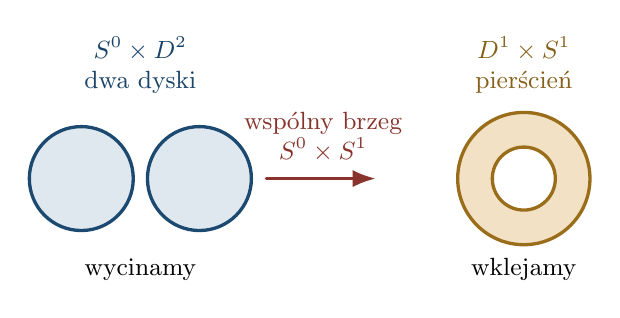
\begin{tikzpicture}[>=Latex,font=\small,line cap=round]
 \node[align=center,manifoldblue!75!black] at (-2.55,1.44)
  {$S^0\times D^2$\\dwa dyski};
 \fill[manifoldblue!14] (-3.30,0) circle (.66);
 \fill[manifoldblue!14] (-1.80,0) circle (.66);
 \draw[manifoldblue!80!black,very thick]
  (-3.30,0) circle (.66) (-1.80,0) circle (.66);
 \node at (-2.55,-1.15) {wycinamy};
 \draw[->,very thick,manifoldred!80!black] (-.95,0)--(.44,0);
 \node[align=center,manifoldred!80!black] at (-.23,.53)
   {wspólny brzeg\\$S^0\times S^1$};
 \begin{scope}[shift={(2.32,0)}]
  \fill[even odd rule,manifoldgold!27]
      (0,0) circle (.84) (0,0) circle (.40);
  \draw[manifoldgold!75!black,very thick]
      (0,0) circle (.84) (0,0) circle (.40);
 \end{scope}
 \node[align=center,manifoldgold!65!black] at (2.32,1.44)
  {$D^1\times S^1$\\pierścień};
 \node at (2.32,-1.15) {wklejamy};
\end{tikzpicture}
\caption{Lokalny model dla $p=0$, $n=2$.
Dwa dyski i pierścień mają ten sam brzeg: dwa okręgi.
Ostateczną rozmaitość otrzymujemy, przyklejając
pierścień do części starej powierzchni pozostałej
po wycięciu dysków. Globalny przykład $S^2\to T^2$
widzieliśmy na Rysunku~\ref{fig:chirurgia-sfera-torus-18}.}
\label{fig:krok-chirurgii-21}
\end{figure}

\begin{przyklad}[Dwie sfery, dwa uchwyty]
\label{prz:dwie-sfery-dwa-uchwyty-21}
\index{chirurgia!powierzchni}
Zacznijmy od $M_0=S^2\sqcup S^2$. Wybieramy po jednym
dysku na każdej składowej. Po ich wycięciu zostają dwa
dyski $D^2\sqcup D^2$; wklejenie pierścienia
$D^1\times S^1$ łączy ich okrągłe brzegi. Wynikiem
pierwszej chirurgii typu $(0,2)$ jest więc $M_1\cong S^2$.
Na tej już połączonej powierzchni wybieramy dwa nowe,
rozłączne dyski. Ich wycięcie pozostawia pierścień
$S^1\times[0,1]$. Po wklejeniu drugiego pierścienia
w sposób zachowujący orientowalność otrzymujemy
$M_2\cong S^1\times S^1=T^2$.
Przy sklejeniu zmieniającym orientowalność powstaje
butelka Kleina, także o charakterystyce Eulera zero.

Każdy krok zmniejsza charakterystykę Eulera o dwa,
bo wycina dwa dyski o łącznej charakterystyce dwa,
a wkleja pierścień o charakterystyce zero. Liczby
składowych i charakterystyki wynoszą odpowiednio
$(b_0,\chi)=(2,4),(1,2),(1,0)$.
Drugi krok jest tym samym przejściem $S^2\to T^2$,
które pokazuje Rysunek~\ref{fig:chirurgia-sfera-torus-18};
wykonany bez pierwszego kroku daje przykład chirurgii
na jednej sferze. W trójwymiarowym śladzie każdej operacji
dołączamy $1$-uchwyt $D^1\times D^2$, a na jego nowym
brzegu pojawia się pobocznica $D^1\times S^1$.
Wallace nazywa ten zabieg \emph{modyfikacją sferyczną}
typu $(0,1)$; nasza para $(0,2)$ zapisuje w drugim miejscu
wymiar dysku normalnego $q$, a nie wymiar sfery wklejanej
\href{https://doi.org/10.4153/CJM-1960-045-7}
{(A.~H.~Wallace, \emph{Modifications and Cobounding Manifolds},
\S\S1 i 3)}.
\end{przyklad}

\begin{figure}[htbp]
\centering
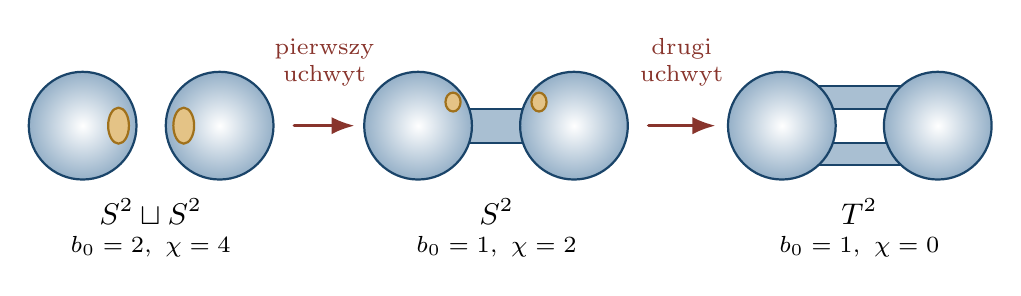
\begin{tikzpicture}[>=Latex,font=\small,line cap=round,
                    scale=1.20,transform shape]
 % Dwie osobne kule: na każdej zaznaczony jest jeden dysk.
 \foreach \x in {-4.70,-3.25}{
  \shade[inner color=white,outer color=manifoldblue!48]
    (\x,0) circle (.57);
  \draw[manifoldblue!75!black,thick] (\x,0) circle (.57);
 }
 \fill[manifoldgold!55] (-4.32,0) ellipse (.11 and .19);
 \fill[manifoldgold!55] (-3.63,0) ellipse (.11 and .19);
 \draw[manifoldgold!78!black,thick]
   (-4.32,0) ellipse (.11 and .19)
   (-3.63,0) ellipse (.11 and .19);

 % Pierwszy uchwyt łączy kule: brzeg bryły jest nadal sferą.
 \fill[manifoldblue!39] (-1.15,-.18) rectangle (.50,.18);
 \draw[manifoldblue!75!black,thick]
   (-1.15,-.18)--(.50,-.18)
   (-1.15,.18)--(.50,.18);
 \foreach \x in {-1.15,.50}{
  \shade[inner color=white,outer color=manifoldblue!48]
    (\x,0) circle (.57);
  \draw[manifoldblue!75!black,thick] (\x,0) circle (.57);
 }
 \fill[manifoldgold!55] (-.78,.25) ellipse (.08 and .10);
 \fill[manifoldgold!55] (.13,.25) ellipse (.08 and .10);
 \draw[manifoldgold!78!black,thick]
   (-.78,.25) ellipse (.08 and .10)
   (.13,.25) ellipse (.08 and .10);

 % Drugi uchwyt tworzy pętlę; białe pole między rurkami jest otworem.
 \foreach \y in {-.30,.30}{
  \fill[manifoldblue!39] (2.70,\y-.12) rectangle (4.35,\y+.12);
  \draw[manifoldblue!75!black,thick]
    (2.70,\y-.12)--(4.35,\y-.12)
    (2.70,\y+.12)--(4.35,\y+.12);
 }
 \foreach \x in {2.70,4.35}{
  \shade[inner color=white,outer color=manifoldblue!48]
    (\x,0) circle (.57);
  \draw[manifoldblue!75!black,thick] (\x,0) circle (.57);
 }

 \draw[->,manifoldred!80!black,very thick]
   (-2.46,0)--(-1.82,0);
 \draw[->,manifoldred!80!black,very thick]
   (1.29,0)--(2.00,0);
 \node[manifoldred!80!black,font=\scriptsize,align=center]
   at (-2.14,.67) {pierwszy\\uchwyt};
 \node[manifoldred!80!black,font=\scriptsize,align=center]
   at (1.64,.67) {drugi\\uchwyt};
 \node at (-3.98,-.91) {$S^2\sqcup S^2$};
 \node at (-.32,-.91) {$S^2$};
 \node at (3.52,-.91) {$T^2$};
 \node[font=\scriptsize] at (-3.98,-1.28) {$b_0=2,\ \chi=4$};
 \node[font=\scriptsize] at (-.32,-1.28) {$b_0=1,\ \chi=2$};
 \node[font=\scriptsize] at (3.52,-1.28) {$b_0=1,\ \chi=0$};
\end{tikzpicture}
\caption{Dwa kolejne uchwyty indeksu jeden dołączone do brył
trójwymiarowych; podpisy pod rysunkami podają topologię ich
brzegów. Złote pola wskazują dyski wycinane w następnym kroku.
Pierwszy uchwyt łączy składowe, drugi tworzy otwór.
W obu krokach sklejanie zachowuje orientowalność.}
\label{fig:dwie-sfery-dwa-uchwyty-21}
\end{figure}

\begin{przyklad}[Zawęźlony torus jako wynik chirurgii]
\label{prz:knotted-torus-surgery-21}
W poprzednim rysunku liczyliśmy zmianę
\emph{abstrakcyjnej} powierzchni. Możemy
również kontrolować jej zanurzenie w $\R^3$.
Niech $K\subset\R^3$ będzie gładkim węzłem
trójlistnym, na przykład obrazem krzywej
\[
 t\longmapsto(\sin t+2\sin2t,
 \cos t-2\cos2t,\sin3t),
 \qquad 0\leq t\leq2\pi.
\]
Wybierzmy małą kulę $B^3$, która zawiera
tylko krótki łuk $K$. Pozostałą część $K$
pogrubiamy do wąskiej rurki $D^1\times D^2$
i jej oba końce przyklejamy do dwóch dysków
w $\partial B^3$. Otrzymujemy pełny torus
$B^3\cup(D^1\times D^2)$ będący otoczeniem
rurkowym $N(K)$. Na jego brzegu operacja jest
dokładnie chirurgią $S^2\to T^2$ z
Rysunku~\ref{fig:krok-chirurgii-21}:
usuwamy dwa dyski $S^0\times D^2$
i wklejamy pobocznicę rurki $D^1\times S^1$.
Jeśli rdzeń uchwytu jest zawęźlony,
otrzymujemy \emph{zawęźlony torus}
$T_K=\partial N(K)\subset\R^3$.
Jako samodzielna powierzchnia nadal jest
homeomorficzny ze zwykłym $T^2$; różni się
położeniem w przestrzeni i dopełnieniem.
\end{przyklad}

\begin{figure}[htbp]
\centering
\begin{tikzpicture}[line cap=round,font=\small]
 \def\knotpath#1#2{plot[domain=#1:#2,samples=180]
  ({.48*(sin(\x)+2*sin(2*\x))},
   {.48*(cos(\x)-2*cos(2*\x))})}
 \begin{scope}[shift={(-4.15,0)}]
  \node[manifoldblue!75!black] at (0,2.05)
    {$\partial B^3=S^2$};
  \shade[inner color=white,outer color=manifoldblue!38]
    (0,0) circle (.94);
  \draw[manifoldblue!76!black,thick] (0,0) circle (.94);
  \fill[manifoldgold!43] (-.38,-.09) ellipse (.17 and .28);
  \fill[manifoldgold!43] (.38,-.09) ellipse (.17 and .28);
  \draw[manifoldgold!75!black,thick]
    (-.38,-.09) ellipse (.17 and .28)
    (.38,-.09) ellipse (.17 and .28);
  \node[font=\scriptsize] at (0,-1.42)
    {dwa dyski $S^0\times D^2$};
 \end{scope}
 \draw[-{Latex[length=2.5mm]},manifoldred!80!black,
    line width=1.1pt] (-2.90,0)--(-1.70,0);
 \begin{scope}
  \node[manifoldblue!75!black] at (0,2.05)
    {rdzeń: węzeł $K$};
  \draw[manifoldblue!76!black,line width=2.0pt]
    \knotpath{0}{360};
  \foreach \a/\b in {8/23,128/143,248/263}{
   \draw[white,line width=6.5pt] \knotpath{\a}{\b};
   \draw[manifoldblue!76!black,line width=2.0pt]
     \knotpath{\a}{\b};
  }
  \draw[manifoldgold!78!black,dashed,thick]
    (0,-.48) circle (.29);
  \node[manifoldgold!60!black,font=\scriptsize,
    anchor=north west] at (.30,-.62) {$B^3$};
 \end{scope}
 \draw[-{Latex[length=3mm]},manifoldred!80!black,
    line width=1.2pt] (1.70,0)--(3.10,0);
 \node[manifoldred!80!black,font=\scriptsize,
   align=center] at (2.40,1.30) {pogrubiamy\\łuk};
 \begin{scope}[shift={(4.55,0)}]
  \node[manifoldblue!75!black] at (0,2.05)
    {$T_K=\partial N(K)$};
  \draw[manifoldblue!75!black,line width=17pt]
    \knotpath{0}{360};
  \draw[manifoldblue!25,line width=14pt]
    \knotpath{0}{360};
  \foreach \a/\b in {8/23,128/143,248/263}{
   \draw[white,line width=21pt] \knotpath{\a}{\b};
   \draw[manifoldblue!75!black,line width=17pt]
     \knotpath{\a}{\b};
   \draw[manifoldblue!25,line width=14pt]
     \knotpath{\a}{\b};
  }
 \end{scope}
\end{tikzpicture}
\caption{Przestrzenny przykład operacji z
Rysunku~\ref{fig:krok-chirurgii-21}.
Najpierw zaznaczamy dwa dyski na sferze.
W środku widać rzut węzła trójlistnego;
białe przerwy oznaczają przejścia pod spodem,
a złoty okrąg małą kulę wokół fragmentu rdzenia.
Po prawej pogrubiona pozostała część węzła
jest $1$-uchwytem przyklejonym do kuli;
jej brzeg to zawęźlony torus.}
\label{fig:knotted-torus-surgery-21}
\end{figure}

\begin{przyklad}[Przeplatanie dwóch uchwytów sfery]
\label{prz:przeplatanie-dwoch-uchwytow-21}
Niech $H=B^3\cup h_A\cup h_B$, gdzie $h_A$ i $h_B$ są
dwoma rozłącznymi $1$-uchwytami $D^1\times D^2$ przyklejonymi
do czterech rozłącznych dysków w $\partial B^3$.
Brzeg $\partial H$ jest orientowalną powierzchnią rodzaju dwa,
którą oznaczymy $\Sigma_2$. Przecinamy pobocznicę każdego
uchwytu wzdłuż jednego okręgu meridionalnego.
Otrzymujemy cztery wolne obrzeża: $A_-,A_+$ oraz $B_-,B_+$.
Pozostała część powierzchni jest sferą z czterema otworami.

Teraz prowadzimy dwie wolne rurki w przestrzeni tak, by w rzucie
minęły się dwa razy: najpierw $A$ przechodzi przed $B$,
a potem $B$ przed $A$.
Jest to pełny skręt dwóch pasm, czyli czysty warkocz
$\sigma_1^2$: pasmo $A$ wraca do swojego kanału, podobnie
pasmo $B$. Sklejamy $A_-$ z $A_+$ i $B_-$ z $B_+$,
zgodnie z pierwotną orientacją każdej rurki. W miejscach
skrzyżowań na rysunku rurki są rozłączne w $\R^3$.

Cięcie wzdłuż okręgów nie zmienia charakterystyki Eulera.
Sfera z czterema otworami ma $\chi=2-4=-2$;
każda z dwóch wklejanych pobocznic jest pierścieniem
o $\chi=0$. Zatem po sklejeniu wciąż mamy spójną,
orientowalną powierzchnię zamkniętą o $\chi=-2$,
a więc $\Sigma_2$. Rysunek określa przebieg zaznaczonych
uchwytów w przestrzeni. Samo przeplecenie ich rdzeni nie
rozstrzyga, czy powierzchnia jako \emph{nieoznaczone}
zanurzenie jest nieizotopijna z wyjściową: nawet
niezawęźlone ciało uchwytowe może mieć szkielet z
przeplecionymi rdzeniami
\href{https://people.dm.unipi.it/benedett/Expositiones_online.pdf}
{(R.~Benedetti, R.~Frigerio i R.~Ghiloni,
\emph{The topology of Helmholtz domains}, przykład 6.16)}.
\end{przyklad}

\begin{figure}[H]
\centering
\begin{tikzpicture}[font=\small,line cap=round,
                    scale=1.04,transform shape]
 % Każda bryła ma cztery osobne stopy uchwytów na tej samej sferze.
 \def\bodyball{%
  \shade[inner color=white,outer color=manifoldblue!52]
    (0,-1.16) ellipse (1.50 and .96);
  \draw[manifoldblue!77!black,thick]
    (0,-1.16) ellipse (1.50 and .96);
 }
 \def\tube#1{%
  \draw[manifoldblue!78!black,line width=13pt] #1;
  \draw[manifoldblue!30,line width=10pt] #1;
  \draw[white,opacity=.42,line width=2.1pt] #1;
 }
 \def\stemAleft{(-1.13,-.73) .. controls (-1.75,-.47) and
   (-1.70,.91) .. (-1.30,1.25)}
 \def\stemAright{(1.30,1.25) .. controls (1.70,.91) and
   (1.75,-.47) .. (1.13,-.73)}
 \def\stemBleft{(-.83,-1.02) .. controls (-1.47,-.80) and
   (-1.53,.12) .. (-1.30,.45)}
 \def\stemBright{(1.30,.45) .. controls (1.53,.12) and
   (1.47,-.80) .. (.83,-1.02)}
 \def\feet{%
  \foreach \x/\y in {-1.13/-.73,1.13/-.73,-.83/-1.02,.83/-1.02}{
   \draw[manifoldblue!68!black,line width=.7pt]
      (\x,\y) ellipse (.10 and .16);
  }
 }
 % Pierwszy stan: dwie równoległe, rozłączne rurki.
 \begin{scope}[shift={(-4.80,0)}]
  \bodyball
  \tube{\stemAleft}
  \tube{\stemAright}
  \tube{(-1.30,1.25)--(1.30,1.25)}
  \tube{\stemBleft}
  \tube{\stemBright}
  \tube{(-1.30,.45)--(1.30,.45)}
  \feet
  \node[manifoldblue!75!black] at (0,1.83) {$\partial H=\Sigma_2$};
  \node[align=center] at (0,-2.55) {dwa rozłączne\\uchwyty};
 \end{scope}
 % Dwa cięcia dają cztery otwarte, złote obrzeża.
 \begin{scope}
  \bodyball
  \tube{\stemAleft}
  \tube{\stemAright}
  \tube{\stemBleft}
  \tube{\stemBright}
  \tube{(-1.30,1.25)--(-.28,1.25)}
  \tube{(.28,1.25)--(1.30,1.25)}
  \tube{(-1.30,.45)--(-.28,.45)}
  \tube{(.28,.45)--(1.30,.45)}
  \foreach \x/\y in {-.28/1.25,.28/1.25,-.28/.45,.28/.45}{
   \fill[white] (\x,\y) ellipse (.055 and .135);
   \draw[manifoldgold!75!black,line width=1.3pt]
     (\x,\y) ellipse (.055 and .135);
  }
  \feet
  \node[manifoldgold!63!black,font=\scriptsize]
    at (-.42,1.63) {$A_-$};
  \node[manifoldgold!63!black,font=\scriptsize]
    at (.42,1.63) {$A_+$};
  \node[manifoldgold!63!black,font=\scriptsize]
    at (-.42,.08) {$B_-$};
  \node[manifoldgold!63!black,font=\scriptsize]
    at (.42,.08) {$B_+$};
  \node[align=center] at (0,-2.55) {cztery obrzeża\\po przecięciu};
 \end{scope}
 % Ponowne połączenie z pełnym skrętem: dwa przecięcia tylko w rzucie.
 \begin{scope}[shift={(4.80,0)}]
  \bodyball
  \tube{\stemAleft}
  \tube{\stemAright}
  \tube{\stemBleft}
  \tube{\stemBright}
  \def\strandA#1#2{plot[domain=#1:#2,samples=90]
    (\x,{.85+.40*cos(360*(\x+1.30)/2.60)})}
  \def\strandB#1#2{plot[domain=#1:#2,samples=90]
    (\x,{.85-.40*cos(360*(\x+1.30)/2.60)})}
  \tube{\strandA{-1.30}{1.30}}
  \tube{\strandB{-1.30}{1.30}}
  % Pierwsze przejście: A z przodu; drugie: B z przodu.
  \draw[white,line width=18pt] \strandA{-.80}{-.50};
  \tube{\strandA{-.89}{-.41}}
  \draw[white,line width=18pt] \strandB{.50}{.80};
  \tube{\strandB{.41}{.89}}
  \feet
  \node[manifoldblue!75!black] at (0,1.83) {$\partial H'=\Sigma_2$};
  \node[align=center] at (0,-2.55) {te same pary końców\\po przepleceniu};
 \end{scope}
 \draw[-{Latex[length=2.5mm]},manifoldred!80!black,
       line width=1.1pt] (-2.95,-.30)--(-2.19,-.30);
 \node[manifoldred!80!black,font=\scriptsize]
   at (-2.57,.03) {tnij};
 \draw[-{Latex[length=2.5mm]},manifoldred!80!black,
       line width=1.1pt] (2.19,-.30)--(2.95,-.30);
 \node[manifoldred!80!black,font=\scriptsize,align=center]
   at (2.57,.15) {zapleć\\i sklej};
\end{tikzpicture}
\caption{Sfera z dwoma rozłącznymi trójwymiarowymi $1$-uchwytami.
Po rozcięciu pobocznic złote pierścienie wskazują cztery
wolne obrzeża. Dwie rury przechodzą nad sobą na przemian
w dwóch miejscach rzutu, bez stykania się w przestrzeni;
każda wraca do swojej pierwotnej pary końców.
Po wygładzeniu sklejeń brzeg nadal jest powierzchnią rodzaju dwa.}
\label{fig:przeplatanie-dwoch-uchwytow-21}
\end{figure}

\begin{uwaga}[Dlaczego nie powstaje rogata sfera?]
Rogata sfera Alexandra jest topologicznie
$S^2$, lecz jej zanurzenie w $\R^3$ nie jest
lokalnie płaskie na zbiorze punktów granicznych
rogów. Każdy \emph{skończony} ciąg opisanych
tutaj gładkich dołączeń uchwytów ma gładki,
a więc lokalnie płaski brzeg. Rogata sfera
powstaje jako granica nieskończonego
powtarzania zazębiających się rogów, nie
jako jeden krok gładkiej chirurgii. Dla
jej konstrukcji i analizy dopełnienia zob.
\href{https://people.mpim-bonn.mpg.de/aruray/documents/top_manifolds.pdf}
{\emph{Topological Manifolds}, §5.2}.
\end{uwaga}

\begin{uwaga}[Dlaczego obramowanie ma znaczenie?]
Z trywialności wiązki normalnej wynika \emph{możliwość}
wyboru $e$, ale nie jego jednoznaczność.
Dwa obramowania różnią się odwzorowaniem
$S^p\to O(q)$ (po ustaleniu zanurzenia rdzenia).
Wymiana kawałków w~\eqref{eq:chirurgia-21} może więc
dać różne wyniki. W szczególności dla okręgu
w $3$-rozmaitości obramowania określają liczby
całkowite, gdyż $\pi_1(SO(2))\cong\Z$;
to źródło różnych wyników chirurgii na węźle.
Jeśli zaś wiązka normalna jest nietrywialna,
nie istnieje nawet zanurzenie $S^p\times D^q$
odpowiadające jej całej tubie.
Na przykład diagonalna sfera $\Delta\subset S^2\times S^2$
ma wiązkę normalną izomorficzną z $TS^2$,
o liczbie Eulera $2$; nie można wykonać na niej
chirurgii wymagającej iloczynowego otoczenia
$S^2\times D^2$.
\end{uwaga}

\section{Ślad chirurgii, odwrotność i dualny uchwyt}
\label{sec:slad-chirurgii-21}

\begin{definicja}[Ślad chirurgii]
\index{slad chirurgii@Ślad chirurgii}
\label{def:slad-chirurgii-21}
\emph{Śladem} operacji $e$ nazywamy $(n+1)$-wymiarowy
kobordyzm
\begin{equation}\label{eq:slad-chirurgii-21}
 W_e=(M\times[0,1])\cup_{e\times\{1\}}
        (D^{p+1}\times D^q).
\end{equation}
Po wygładzeniu naroży ma on brzeg wejściowy $M$
i brzeg wyjściowy $M_e$.
\end{definicja}

\begin{twierdzenie}[Ślad i chirurgia odwrotna]
\label{thm:odwrotna-chirurgia-21}
Ślad~\eqref{eq:slad-chirurgii-21} powstaje przez
dołączenie jednego uchwytu indeksu $p+1$.
Oglądany od strony $M_e$ jest śladem chirurgii
na obramowanej sferze $S^{q-1}\subset M_e$,
o uchwycie indeksu $q=n-p$.
Ta druga chirurgia przywraca $M$.
\end{twierdzenie}
\begin{proof}
Uchwyt w~\eqref{eq:slad-chirurgii-21} ma postać
$D^{p+1}\times D^q$. Jego część przyklejona do
$M\times\{1\}$ to $\partial D^{p+1}\times D^q
=S^p\times D^q$, więc indeks uchwytu wynosi $p+1$.
Niewykorzystana część jego brzegu to
$D^{p+1}\times\partial D^q=D^{p+1}\times S^{q-1}$;
wraz z pozostałą częścią $M$ daje dokładnie
wzór~\eqref{eq:chirurgia-21}.

Po odwróceniu kierunku kobordyzmu część
$D^{p+1}\times S^{q-1}$ jest obszarem
przyczepienia \emph{dualnego} uchwytu
$D^q\times D^{p+1}$. Sferą rdzenia w nowym
brzegu jest $\{0\}\times S^{q-1}$, a obramowaniem
jej normalnych dysków jest czynnik $D^{p+1}$.
Wycinamy więc $D^{p+1}\times S^{q-1}$
i przywracamy $S^p\times D^q$.
Wymiar uchwytu dualnego wynosi
$(n+1)-(p+1)=q$, zgodnie z
Twierdzeniem~\ref{thm:dualny-uchwyt-18}.
\end{proof}

\begin{figure}[htbp]
\centering
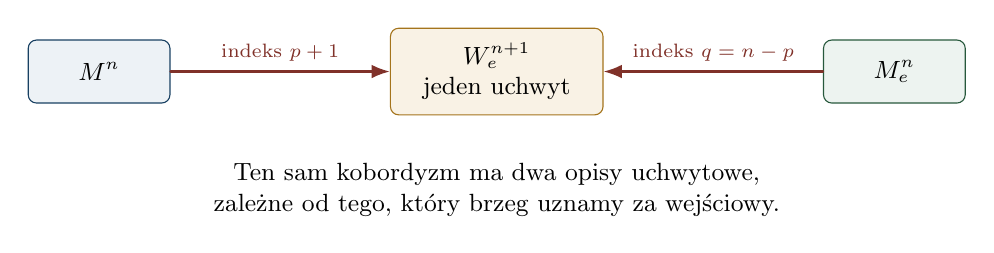
\begin{tikzpicture}[>=Latex,font=\small,line cap=round]
 \node[draw=manifoldblue!70!black,rounded corners=3pt,
  fill=manifoldblue!8,minimum width=1.8cm,minimum height=.8cm]
  (M) at (-5.05,0) {$M^n$};
 \node[draw=manifoldgold!80!black,rounded corners=3pt,
  fill=manifoldgold!12,minimum width=2.7cm,minimum height=1.1cm,
  align=center] (W) at (0,0) {$W_e^{n+1}$\\jeden uchwyt};
 \node[draw=manifoldgreen!70!black,rounded corners=3pt,
  fill=manifoldgreen!9,minimum width=1.8cm,minimum height=.8cm]
  (N) at (5.05,0) {$M_e^n$};
 \draw[->,thick,manifoldred!75!black]
  (M) -- node[above,font=\scriptsize] {indeks $p+1$} (W);
 \draw[->,thick,manifoldred!75!black]
  (N) -- node[above,font=\scriptsize] {indeks $q=n-p$} (W);
 \node[align=center,text width=10cm] at (0,-1.5)
  {Ten sam kobordyzm ma dwa opisy uchwytowe,
   zależne od tego, który brzeg uznamy za wejściowy.};
\end{tikzpicture}
\caption{Ślad chirurgii od strony starego i nowego brzegu.
Różnica indeksów nie oznacza dwóch różnych kobordyzmów.}
\label{fig:slad-chirurgii-21}
\end{figure}

\section{Jak chirurgia zmienia niezmienniki}
\label{sec:niezmienniki-chirurgia-21}

W tej sekcji $M$ jest spójna i zamknięta.
Ślad pozwala obliczyć zmianę bez zgadywania
topologii $M_e$ z samego rysunku.

\begin{twierdzenie}[Względna homologia śladu]
\label{thm:homologia-sladu-21}
Dla śladu $W_e$ mamy
\[
 H_i(W_e,M;\Z)\cong
 \begin{cases}\Z,&i=p+1,\\0,&i\ne p+1,
 \end{cases}
 \qquad
 H_i(W_e,M_e;\Z)\cong
 \begin{cases}\Z,&i=q,\\0,&i\ne q.
 \end{cases}
\]
Odpowiadające ciągi dokładne określają wpływ
chirurgii na homologię obu brzegów.
\end{twierdzenie}
\begin{proof}
Obcięcie $M\times[0,1]$ w kierunku przedziału
nie zmienia homologii. Z twierdzenia o wycinaniu
względny kompleks pary $(W_e,M)$ ma homologię
pary
\[
 (D^{p+1}\times D^q,S^p\times D^q).
\]
Projekcja w pierwszy czynnik jest homotopijną
równoważnością par z $(D^{p+1},S^p)$:
odkształcamy $D^q$ do środka, zachowując
$S^p\times D^q$. Iloraz $D^{p+1}/S^p$
jest sferą $S^{p+1}$, więc homologia względna
wynosi $\Z$ tylko w stopniu $p+1$.

Po odwróceniu śladu przyczepiamy do $M_e$
uchwyt indeksu $q$. Ten sam argument daje
$(W_e,M_e)\simeq(D^q,S^{q-1})$ na poziomie
homologii względnej i drugą formułę.
Ciąg dokładny pary, na przykład,
\[
 \cdots\longrightarrow H_{p+1}(M)
 \longrightarrow H_{p+1}(W_e)
 \longrightarrow\Z\xrightarrow{\partial}
 H_p(M)\longrightarrow H_p(W_e)
 \longrightarrow0,
\]
pokazuje konkretnie, że generator nowego
względnego $(p+1)$-dysku ma na brzegu klasę
rdzenia $[e(S^p\times\{0\})]$.
Analogiczny ciąg względem $M_e$ opisuje
sferę dualną. Nie wolno z samego wyrażenia
$H_{p+1}(W_e,M)=\Z$ wnioskować, że zawsze
ubywa generator w $H_p(M)$: jeśli klasa rdzenia
jest zerowa, nowy dysk może zamiast tego
tworzyć klasę w $H_{p+1}(W_e)$.
\end{proof}

\begin{stwierdzenie}[Zmiana charakterystyki Eulera]
\label{prop:euler-chirurgia-21}
Dla $M$ zamkniętej zachodzi
\begin{equation}\label{eq:euler-chirurgia-21}
 \chi(M_e)-\chi(M)
 =(-1)^{q-1}-(-1)^p
 =\begin{cases}
    0,&n\text{ nieparzyste},\\
    -2(-1)^p,&n\text{ parzyste}.
   \end{cases}
\end{equation}
\end{stwierdzenie}
\begin{proof}
Oznaczmy przez $C$ część $M$ pozostałą
po usunięciu wnętrza $S^p\times D^q$.
Z addytywności charakterystyki Eulera przy
sklejaniu wzdłuż podkompleksu wspólne wyrazy
$\chi(C)$ i $\chi(S^p\times S^{q-1})$ redukują się.
Pozostaje
\[
 \chi(M_e)-\chi(M)
 =\chi(D^{p+1}\times S^{q-1})
  -\chi(S^p\times D^q)
 =(1+(-1)^{q-1})-(1+(-1)^p).
\]
Ponieważ $q=n-p$, przy nieparzystym $n$
wykładniki $q-1$ i $p$ mają tę samą parzystość,
a przy parzystym przeciwną. To daje
ostatnią postać~\eqref{eq:euler-chirurgia-21}.
\end{proof}

\begin{twierdzenie}[Wpływ na $\pi_1$ przy kowymiarze co najmniej trzy]
\label{thm:pi1-chirurgia-21}
Jeśli $q=n-p\geq3$, to inkluzja $M_e\hookrightarrow W_e$
indukuje izomorfizm na $\pi_1$. Ponadto:
\begin{enumerate}[label=(\alph*)]
\item dla $p\geq2$ obie inkluzje brzegów indukują
izomorfizmy na $\pi_1$;
\item dla $p=1$ mamy
$\pi_1(M_e)\cong\pi_1(M)/\langle\!\langle[e(S^1)]\rangle\!\rangle$;
\item dla $p=0$ (obie kule leżą w spójnej $M$)
$\pi_1(M_e)\cong\pi_1(M)*\Z$.
\end{enumerate}
Przez $\langle\!\langle\gamma\rangle\!\rangle$
oznaczamy najmniejszą podgrupę normalną
zawierającą $\gamma$.
\end{twierdzenie}
\begin{proof}
Ślad ma typ homotopijny $M$ z jedną dołączoną
komórką wymiaru $p+1$: czynnik $D^q$ uchwytu
jest ściągalny, a mapa przyczepienia to rdzeń $S^p$.
Dla $p\geq2$ dołączenie komórki wymiaru
co najmniej $3$ nie zmienia grupy podstawowej
(twierdzenie van Kampena lub przybliżanie pętli
i homotopii przez komórki wymiaru $2$).
Dla $p=1$ dołączenie $2$-komórki dodaje relację
$[e(S^1)]=1$ wraz ze wszystkimi jej sprzężeniami,
co daje iloraz z punktu (b). Dla $p=0$
dołączamy odcinek z końcami w tej samej spójnej
składowej $M$. Po wyborze drogi łączącej końce
otrzymujemy dodatkową pętlę niezależną od
poprzednich, więc van Kampen daje iloczyn wolny
z $\Z$.

Od strony $M_e$ ślad ma jedną komórkę wymiaru
$q\geq3$, gdyż dualny uchwyt ma indeks $q$.
Takie dołączenie nie zmienia $\pi_1$.
Złożenie powyższych obliczeń dowodzi tez.
Bez warunku $q\geq3$ ostatnie zdanie może być
fałszywe: dualny $2$-uchwyt potrafi dodać relację.
\end{proof}

\begin{przyklad}[Sfery przechodzą w produkty sfer]
\label{prz:sfera-produkt-chirurgia-21}
Podzielmy $S^n$ jako brzeg
$D^{p+1}\times D^q$:
\[
 S^n=(S^p\times D^q)
 \cup_{S^p\times S^{q-1}}
 (D^{p+1}\times S^{q-1}).
\]
Wybierzmy standardową sferę $S^p\times\{0\}$
w pierwszym kawałku. Po jej chirurgii pozostaje
$D^{p+1}\times S^{q-1}$ i doklejamy jego
drugi egzemplarz wzdłuż brzegu.
Podwojenie $D^{p+1}$ jest $S^{p+1}$, zatem
\begin{equation}\label{eq:chirurgia-sfery-21}
 (S^n)_e\cong S^{p+1}\times S^{q-1}
 \qquad\text{dla standardowego obramowania.}
\end{equation}
Dla $p=0$ uzyskujemy $S^1\times S^{n-1}$:
operacja \emph{tworzy} generator $\pi_1$.
Dla $n=6$, $p=2$ otrzymujemy
$S^3\times S^3$, którego $H_3$ ma rangę $2$,
mimo że $H_3(S^6)=0$. Chirurgia nie zawsze
usuwa homologię; zależy od położenia rdzenia
i od stopnia operacji.
\end{przyklad}

\begin{przyklad}[Dwa obramowania okręgu w $S^4$]
\label{prz:dwa-obramowania-S1-S4-21}
\index{obramowanie!okręgu w $S^4$}
Weźmy standardowy okrąg $K=S^1\times\{0\}$ w rozkładzie
\[
 S^4=\partial(D^2\times D^3)
    =(S^1\times D^3)\cup_{S^1\times S^2}(D^2\times S^2).
\]
Pierwszy składnik jest jego otoczeniem rurowym. Ustalmy
orientację $K$ i produktowe obramowanie z tego rozkładu.
Każde inne zorientowane obramowanie tej samej wiązki
normalnej rangi $3$ różni się od niego odwzorowaniem
$g:S^1\to SO(3)$. Klasy obramowań są więc elementami
\[
 [S^1,SO(3)]=\pi_1(SO(3))\cong\Z/2.
\]
W szczególności obramowanie produktowe reprezentuje zero,
a drugą klasę reprezentuje pętla $g_1(e^{i\theta})$
obracająca $\R^3$ o kąt $\theta$ wokół ustalonej osi.
Jej podniesienie do dwukrotnego nakrycia
$SU(2)\cong S^3\to SO(3)$ z
Twierdzenia~\ref{thm:su2-so3-cover-lie} zaczyna się w $1$,
a kończy w $-1$, więc pętla nie jest ściągalna.

Chirurgia usuwa $S^1\times\operatorname{int}D^3$
i wkleja $D^2\times S^2$. Pozostała część $S^4$
jest drugą kopią $D^2\times S^2$. Przy sklejeniu
dwóch kopii wzdłuż $S^1\times S^2$ przejście na
włóknie $S^2$ jest działaniem $g$.
Oznaczmy wynik chirurgii przez $M_g$.
Jest to wiązka $S^2$ nad
$D^2\cup_{S^1}D^2=S^2$ o funkcji przejścia $g$.
Dla obramowania produktowego jest to $S^2\times S^2$;
dla $g_1$ jest to nietrywialna zorientowana wiązka
$S^2\widetilde{\times}S^2$.

Policzmy formy przecięcia bez odwoływania się do
klasyfikacji rozmaitości czterowymiarowych.
Niech $F$ oznacza włókno, a $B$ przekrój wiązki.
Przekrój istnieje w obu przypadkach: dla $g_1$
można wybrać punkt osi obrotu. Włókno można
przesunąć do innego włókna, a przekrój przecina
każde włókno raz, więc
$F\cdot F=0$ i $F\cdot B=1$.
W ciągu Mayera--Vietorisa dla dwóch kopii
$D^2\times S^2$ odwzorowanie z
$H_2(S^1\times S^2)\cong\Z$ do
$H_2(D^2\times S^2)^{\oplus2}\cong\Z^2$
ma obraz generowany przez $(1,-1)$.
Dalszy fragment ciągu to
\[
 0\longrightarrow\Z^2/\langle(1,-1)\rangle
 \longrightarrow H_2(M_g;\Z)
 \longrightarrow H_1(S^1\times S^2;\Z)
 \longrightarrow0.
\]
Pierwszy składnik generuje klasa włókna $F$.
Przekrój $B$ przecina wspólny brzeg obu
kopii w pętli $S^1\times\{p\}$; jej klasa
generuje ostatnią grupę $\Z$.
Stąd $H_2(M_g;\Z)\cong\Z^2$
z bazą $(F,B)$.
Przy sklejeniu produktowym przekrój ma trywialną
wiązkę normalną i $B\cdot B=0$. W bazie $(F,B)$
otrzymujemy formę hiperboliczną
\[
 Q_{S^2\times S^2}
   =\begin{pmatrix}0&1\\1&0\end{pmatrix}=H.
\]
W przypadku $g_1$ normalna płaszczyzna do
przekroju przy ustalonym punkcie osi obraca się
o pełny obrót przy obejściu równika. Jej funkcja
przejścia w $SO(2)$ ma stopień $1$, więc jej
liczba Eulera, czyli $B\cdot B$, wynosi $1$
po zgodnym wyborze orientacji. Zatem
\[
 Q_{S^2\widetilde{\times}S^2}
   =\begin{pmatrix}0&1\\1&1\end{pmatrix}
   \quad\text{w bazie $(F,B)$}.
\]
W bazie $(B,B-F)$ ta sama forma ma macierz
$\operatorname{diag}(1,-1)$.
Obie formy mają rząd $2$ i sygnaturę $0$,
ale pierwsza jest parzysta, a druga nieparzysta.
W szczególności wyniki chirurgii nie są homeomorficzne.
Nietrywialna wiązka jest ponadto dyfeomorficzna
z $\mathbb{CP}^2\#\overline{\mathbb{CP}^2}$; tej identyfikacji
nie wyprowadzamy z samej macierzy przecięć.

Dwie możliwości chirurgii standardowego okręgu
w $S^4$ podaje
\href{https://arxiv.org/abs/1502.06834}
{K.\ Larson, \emph{Surgery on tori in the 4-sphere},
dowód propozycji 4.3}. Klasyfikację wiązek przez
$\pi_1(SO(3))$ i identyfikację nietrywialnego
przypadku z rozdmuchaniem $\mathbb{CP}^2$ opisuje
\href{https://www.mathematik.hu-berlin.de/~wendl/pub/rationalRuled.pdf}
{C.\ Wendl, \emph{Holomorphic Curves in Low Dimensions},
przykład 1.11 i uwaga 1.13}.
To rachunek konkretnej chirurgii w wymiarze cztery;
nie używa wysokowymiarowego twierdzenia Walla
o przeszkodzie chirurgicznej.
\end{przyklad}

\section{Odwzorowania normalne: jakie dane zachowujemy?}
\label{sec:normalne-chirurgia-21}

Dotąd zmienialiśmy rozmaitość bez wskazania celu.
W programie chirurgii mamy przestrzeń $X$ i chcemy
poprawić odwzorowanie $f:M\to X$. Najczytelniejsza
wersja wprowadzająca zakłada, że $M^n$ i $X^n$
są spójnymi zamkniętymi \emph{zorientowanymi}
rozmaitościami gładkimi. Wersje z brzegiem
i współczynnikami lokalnymi omówimy później.

\begin{definicja}[Stopień jeden i odwzorowanie normalne]
\index{stopien jeden i odwzorowanie normalne@Stopień jeden i odwzorowanie normalne}
\label{def:normal-map-21}
Odwzorowanie $f:M^n\to X^n$ ma \emph{stopień jeden},
jeśli $f_*[M]=[X]\in H_n(X;\Z)$.
Wybierzmy rzeczywistą wiązkę $\xi\to X$.
\emph{Odwzorowaniem normalnym stopnia jeden}
nazywamy dane $(f,b)$, gdzie $f$ ma stopień jeden,
a $b$ jest stabilnym izomorfizmem wiązek
\begin{equation}\label{eq:normal-map-21}
 b:\nu_M\oplus\varepsilon^a
   \xrightarrow{\ \cong\ }
   f^*\xi\oplus\varepsilon^b
\end{equation}
po dobraniu rang tak, aby obie strony były tej samej
rangi. Tutaj $\nu_M$ oznacza wiązkę normalną
zanurzenia $M$ w przestrzeni euklidesowej,
a $\varepsilon^j$ trywialną wiązkę rangi $j$.
Dwa zanurzenia dają ten sam stabilny typ $\nu_M$.
\end{definicja}

W dalszych rozdziałach dopuszczamy też cel
nieorientowalny. Wtedy wymagamy
$f^*w_1(TX)=w_1(TM)$, czyli zgodności
lokalnych systemów orientacji, i definiujemy
stopień jeden przez
$f_*[M]=[X]$ w
$H_n(X;\Z^{w_X})$; po lewej używamy
$[M]\in H_n(M;\Z^{w_M})$.
Symbol $\Z^{w_X}$ oznacza lokalny system,
w którym pętla odwracająca orientację
działa na $\Z$ przez mnożenie przez $-1$.
Gdy obie rozmaitości są zorientowane,
jest to dokładnie poprzednia definicja.
Ogólna wersja twierdzenia Walla i ciągu
chirurgii korzysta z tej konwencji.

Warunek o stopniu mówi, że $f$ przenosi klasę
fundamentalną bez wielokrotności. Dane $b$ pozwalają
porównywać kierunki normalne nad punktami $M$
z wiązką wybraną nad $X$ i kontrolować obramowania
podczas operacji. Nie każda mapa stopnia jeden
\emph{automatycznie} ma strukturę~\eqref{eq:normal-map-21}
dla z góry ustalonej $\xi$. Gdy $X$ jest
rozmaitością, naturalnym punktem odniesienia jest
$\xi=\nu_X$: identyczność $X\to X$ ma wtedy
oczywiste dane normalne.

\begin{lemat}[Rozszczepienie na homologię celu i jądro]
\label{lem:split-normalne-21}
Jeśli $f:M^n\to X^n$ ma stopień jeden, to
$f_*:H_i(M;\Z)\to H_i(X;\Z)$ jest surjekcją
w każdym stopniu. Istnieje naturalny prawy odwrotny
\[
 f_!=\operatorname{PD}_M\circ f^*
       \circ\operatorname{PD}_X^{-1}:H_i(X;\Z)\to H_i(M;\Z),
 \qquad f_*f_!=\id.
\]
W szczególności
$H_i(M;\Z)\cong f_!H_i(X;\Z)\oplus K_i(f)$,
gdzie $K_i(f)=\ker f_*$.
\end{lemat}
\begin{proof}
Niech $x\in H_i(X;\Z)$ i niech
$\alpha=\operatorname{PD}_X^{-1}(x)
\in H^{n-i}(X;\Z)$.
Z definicji dualności Poincarégo
$f_!(x)=[M]\frown f^*\alpha$.
Naturalność iloczynu z klasą fundamentalną daje
\[
 f_*f_!(x)
 =f_*([M]\frown f^*\alpha)
 =f_*[M]\frown\alpha
 =[X]\frown\alpha=x.
\]
Zatem $f_*$ ma prawy odwrotny. Każde
$z\in H_i(M)$ rozkłada się jawnie jako
\[
 z=f_!(f_*z)+\bigl(z-f_!(f_*z)\bigr),
\]
a drugi składnik leży w $K_i(f)$.
Część wspólna obu składników jest zerowa,
bo $f_*f_!=\id$. Nie używaliśmy tu jeszcze
izomorfizmu wiązek $b$.
\end{proof}

\begin{uwaga}[Czego nie dowodzi ten lemat?]
Znikanie wszystkich $K_i(f)$ dla \emph{zwykłych}
homologii nie wystarcza do stwierdzenia, że $f$
jest równoważnością homotopijną przy dowolnej
$\pi_1(X)$. Dla pełnego kryterium potrzebna
jest kontrola $\pi_1$ oraz homologii nakryć
uniwersalnych, czyli współczynników w
$\Z[\pi_1(X)]$; używa się wówczas odpowiedniej
wersji twierdzenia Whiteheada. To odróżnia
zadanie chirurgii od samego liczenia rang homologii.
\end{uwaga}

\begin{definicja}[Normalna kobordancja]
\index{normalna kobordancja@Normalna kobordancja}
\label{def:normal-bordism-21}
Dwa odwzorowania normalne $(f_0,b_0,\xi_0):M_0\to X$
i $(f_1,b_1,\xi_1):M_1\to X$ są \emph{normalnie
kobordantne}, jeśli istnieje zwarty gładki kobordyzm
$(W;M_0,M_1)$, odwzorowanie $F:W\to X$
o ograniczeniach $f_0,f_1$ oraz wiązka
nad $X\times I$ ze stabilnymi danymi normalnymi
nad $F$, której ograniczenia na końcach dają
$(\xi_0,b_0)$ i $(\xi_1,b_1)$ (z uwzględnieniem
normalnego kierunku kołnierza brzegu).
W szczególności wiązki $\xi_0$ i $\xi_1$
muszą być stabilnie izomorficzne; w klasyfikacji
nie ustalamy jednak z góry jednej wiązki $\xi$.
\end{definicja}

\begin{stwierdzenie}[Stopień nie zmienia się w kobordancji]
\label{prop:stopien-kobordancja-21}
Przy zgodnym wyborze orientacji $W$ i jego brzegów,
tak że
$\partial[W]=[M_1]-[M_0]$, to
$F_*[M_0]=F_*[M_1]\in H_n(X;\Z)$.
\end{stwierdzenie}
\begin{proof}
Na poziomie łańcuchów $F_*(\partial[W])$
jest brzegiem $F_*[W]$, więc przedstawia zero
w homologii $X$. Po podstawieniu
$\partial[W]=[M_1]-[M_0]$ otrzymujemy
$f_{1*}[M_1]-f_{0*}[M_0]=0$.
Zatem jeśli jedno ograniczenie ma stopień jeden,
to drugie także.
\end{proof}

\section{Kiedy chirurgia działa na odwzorowanie?}
\label{sec:normalny-krok-21}

Zwykła operacja~\eqref{eq:chirurgia-21} nie
wystarcza: po zmianie dziedziny musimy nadal
mieć odwzorowanie do $X$ i zgodne dane normalne.

\begin{twierdzenie}[Warunek przedłużenia odwzorowania]
\label{thm:przedluzenie-mapy-21}
Niech $e:S^p\times D^q\hookrightarrow M$ będzie
zanurzeniem obramowanym, $f:M\to X$ ciągłym
odwzorowaniem. Odwzorowanie $f$ przedłuża się
(po homotopii w otoczeniu $e$) do
$F:W_e\to X$ wtedy i tylko wtedy, gdy
\[
 f\circ e|_{S^p\times\{0\}}:S^p\to X
\]
jest nullhomotopijne. Aby przedłużyć także
\emph{dane normalne} $b$ z~\eqref{eq:normal-map-21},
wybrana nullhomotopia i obramowanie $e$
muszą być zgodne ze stabilną trywializacją
nad przyklejanym uchwytem. Dokładniej,
po ustaleniu trywializacji obu wiązek nad
kontraktybilnym uchwytem różnica między
identyfikacjami na części przyczepionej
$S^p\times D^q\simeq S^p$ daje stabilną mapę
$S^p\to O$. Dane normalne przedłużają się
wtedy i tylko wtedy, gdy ta mapa jest
nullhomotopijna.
\end{twierdzenie}
\begin{proof}
Jeżeli $F$ istnieje, ograniczmy je do rdzenia
uchwytu $D^{p+1}\times\{0\}\subset W_e$.
Na jego brzegu dostajemy $f\circ e|_{S^p\times\{0\}}$;
rdzeń jest więc żądaną nullhomotopią.

Odwrotnie, niech $H:D^{p+1}\to X$ przedłuża
to odwzorowanie rdzenia. W otoczeniu
$S^p\times D^q$ odwzorowanie $f\circ e$
jest homotopijne do mapy niezależnej od
współrzędnej $D^q$, przez skurczenie
$z\mapsto(1-t)z$. Własność przedłużania
homotopii dla kołnierza zanurzonej tuby
pozwala zastąpić $f$ mapą homotopijną,
która na obszarze przyczepienia zależy
tylko od $x\in S^p$. Na uchwycie kładziemy
$F(y,z)=H(y)$, $y\in D^{p+1}$, $z\in D^q$.
Formuły zgadzają się na $S^p\times D^q$,
więc sklejają się w mapę całego $W_e$.

Wiązka nad dyskiem $D^{p+1}\times D^q$ jest
trywialna; po stabilizacji wybieramy na niej
ramy. Obramowanie $e$ identyfikuje ramy
normalne na obszarze przyczepienia z ramami
pochodzącymi od $M$. Ich porównanie za pomocą
$b$ jest mapą $S^p\times D^q\to O(r)$
dla dostatecznie dużego $r$. Ponieważ $D^q$
jest ściągalny, mapa ta ma klasę w $\pi_p(O)$.
Przedłużenie na $D^{p+1}\times D^q$ istnieje
dokładnie wtedy, gdy jej ograniczenie do $S^p$
jest nullhomotopijne; wystarczalność daje
rozciągnięcie nullhomotopii radialnie po
$D^{p+1}$, a konieczność jej ograniczenie
z dowolnego przedłużenia.
Inny wybór ram nad dyskiem zmienia porównanie
o mapę przedłużalną, zatem nie zmienia warunku.
Sam fakt, że $H$ istnieje, nie zeruje tej
klasy: warunek normalny jest dodatkowy.
Wtedy wraz z $F$ otrzymujemy normalną
kobordancję do odwzorowania $M_e\to X$.
\end{proof}

\begin{figure}[htbp]
\centering
\begin{tikzpicture}[>=Latex,font=\small]
 \node[draw=manifoldblue!75!black,fill=manifoldblue!9,
    rounded corners=3pt,minimum width=1.9cm,minimum height=.65cm]
    (S) at (-3.35,.92) {$S^p$};
 \node[draw=manifoldgreen!70!black,fill=manifoldgreen!9,
    rounded corners=3pt,minimum width=1.9cm,minimum height=.65cm]
    (M) at (-.25,.92) {$M$};
 \node[draw=manifoldgold!75!black,fill=manifoldgold!11,
    rounded corners=3pt,minimum width=1.9cm,minimum height=.65cm]
    (D) at (-3.35,-.95) {$D^{p+1}$};
 \node[draw=manifoldred!75!black,fill=manifoldred!8,
    rounded corners=3pt,minimum width=1.9cm,minimum height=.65cm]
    (X) at (-.25,-.95) {$X$};
 \draw[->,thick] (S)--node[above] {$e|_{S^p}$} (M);
 \draw[->,thick] (M)--node[right] {$f$} (X);
 \draw[->,thick] (S)--node[left] {brzeg} (D);
 \draw[->,thick,manifoldred!75!black]
    (D)--node[below] {$H$} (X);
 \node[align=left,text width=3.7cm] at (3.3,0)
  {Dysk $H$ wypełnia obraz sfery w $X$.\\
   Zgodne obramowanie pozwala\\
   dołączyć cały uchwyt nad $H$.};
\end{tikzpicture}
\caption{Warunek na odwzorowanie w kroku chirurgii.
Komutatywność diagramu oznacza
$H|_{S^p}=f\circ e|_{S^p\times\{0\}}$.
Dodatkowe dane normalne kontrolują obramowanie.}
\label{fig:normalna-chirurgia-21}
\end{figure}

\begin{przyklad}[Chirurgia nad sferą docelową]
\label{prz:normalna-sfera-21}
Dla standardowej sfery $S^p\subset S^n$, $p<n$,
identyczność $S^n\to S^n$ wysyła ten rdzeń
na sferę nullhomotopijną, ponieważ
$\pi_p(S^n)=0$. Przy standardowym obramowaniu
i zgodnych stabilnych danych normalnych
krok chirurgii daje mapę stopnia jeden
\[
 f':S^{p+1}\times S^{q-1}\longrightarrow S^n
\]
normalnie kobordantną z identycznością.
Możemy też zbudować $f'$ bezpośrednio:
wybieramy mały $n$-dysk w produkcie,
przenosimy go na $S^n$ z zachowaniem
orientacji i zgniatamy do punktu dopełnienie
wnętrza dysku. Otrzymana mapa ma stopień jeden.
Produkt sfer jest stabilnie równoległizowalny
(po dodaniu dwóch prostych trywialnych),
a $S^n$ po dodaniu jednej; dlatego istnieją
zgodne stabilne dane normalne.
Nie twierdzimy, że $f'$ jest równoważnością:
dla $1\leq p\leq n-2$ produkt ma zwykle
niezerową homologię w stopniach pośrednich.
\end{przyklad}

\begin{przyklad}[Ślad od $S^6$ do $S^3\times S^3$]
\label{prz:slad-s6-produkt-21}
Wybierzmy $n=6$, $p=2$ i $q=4$ w
Przykładzie~\ref{prz:sfera-produkt-chirurgia-21}.
Rozkład
\[
 S^6=\partial(D^3\times D^4)
 =(S^2\times D^4)\cup_{S^2\times S^3}
   (D^3\times S^3)
\]
wskazuje standardowo obramowaną sferę
$S^2\times\{0\}$ w pierwszym kawałku.
Jej ślad
\[
 W=(S^6\times I)\cup_{S^2\times D^4}
   (D^3\times D^4)
\]
jest siedmiowymiarowym kobordyzmem z jednym
uchwytem indeksu trzy. Górny brzeg składa się
z dwóch kopii $D^3\times S^3$, więc jest
produktem $M=S^3\times S^3$.

Ponieważ $\pi_2(S^6)=0$, odwzorowanie
$\id_{S^6}$ przedłuża się nad rdzeniem
uchwytu. Ponieważ identyczność jest
$3$-spójna, wybieramy standardowe
przedłużenie danych normalnych z
Lematu~\ref{lem:wall-lokalna-stabilizacja-22}.
Spełnia ono warunek ram z
Twierdzenia~\ref{thm:przedluzenie-mapy-21}
i jest zgodne z produktowymi obramowaniami
obu sfer czynnikowych.
Otrzymujemy normalny ślad $F:W\to S^6\times I$,
którego górnym brzegiem jest mapa normalna
$(f,b):M\to S^6$ stopnia jeden. Symbol $b$
oznacza ten standardowy wybór danych ze śladu.

W nowo dołączonej połowie $D^3\times S^3$
sfera $B=\{0\}\times S^3$ ma obramowane
otoczenie $D^3\times S^3$. Oglądany od strony
$M$ ślad $W$ dołącza do $B$ uchwyt indeksu
cztery i odzyskuje $S^6$, zgodnie z
Twierdzeniem~\ref{thm:odwrotna-chirurgia-21}.
Jądro mapy $f$ policzymy w
Przykładzie~\ref{prz:forma-produkt-21}, a jej
miejsce w ciągu chirurgii wskaże
Przykład~\ref{prz:slad-s6-ciag-23}.
\end{przyklad}

\section{Jądra chirurgii i próg wymiaru środkowego}
\label{sec:jadra-chirurgii-21}

Dla odwzorowania normalnego stopnia jeden
piszemy $K_i(f)=\ker(H_i(M;\Z)\to H_i(X;\Z))$.
Intuicyjnie są to klasy, które dziedzina ma
\emph{nadmiarowo} w porównaniu z celem.
Nie każdą z nich można usunąć: trzeba ją
zrealizować przez zanurzoną sferę z obramowaniem,
po której obraz w $X$ da się wypełnić dyskiem.
Obramowanie musi ponadto pasować do danych
normalnych. W wyższych wymiarach pozycja ogólna
i trik Whitneya pozwalają realizować wiele
takich operacji poniżej wymiaru środkowego;
przy wymiarze środkowym sfery spotykają się
i pojawia się dodatkowy rachunek przecięć.

\subsection*{Co dokładnie usuwa trik Whitneya?}
\index{trik Whitneya@Trik Whitneya}
Niech $A^p$ i $B^q$ będą zorientowanymi,
poprzecznie zanurzonymi podrozmaitościami
w zorientowanej $N^n$, gdzie $p+q=n$.
Zakładamy $p,q\geq1$.
Ich przecięcia są izolowanymi punktami ze znakami.
Wybierzmy dwa punkty $x_-,x_+\in A\cap B$
o przeciwnych znakach oraz zanurzone łuki
$a\subset A$ od $x_-$ do $x_+$
i $b\subset B$ wracający do $x_-$.
Ich wnętrza omijają drugi płat i wszystkie
inne punkty przecięcia, a $a\cap b=\{x_-,x_+\}$.
Tworzą \emph{okrąg Whitneya} $a\cup b$.
Samo równanie $(-1)+(+1)=0$ nie daje jeszcze
izotopii: potrzebny jest dysk wypełniający ten
okrąg w odpowiednim położeniu.

\begin{stwierdzenie}[Lokalny ruch Whitneya]
\label{prop:lokalny-Whitney-21}
Załóżmy, że $a\cup b$ ogranicza gładko zanurzony
dysk $D_W\subset N$ o wnętrzu rozłącznym z
$A\cup B$. Załóżmy także, że dysk ma
\emph{obramowanie Whitneya}: normalne kierunki
indukowane wzdłuż $a$ i $b$ przez oba płaty
przedłużają się bez skręcenia nad $D_W$.
Wówczas lokalna izotopia jednego z płatów,
wsparta w otoczeniu $D_W$, usuwa $x_-,x_+$
bez tworzenia nowych przecięć $A\cap B$.
\end{stwierdzenie}
\begin{proof}
Obramowanie daje produktowe otoczenie dysku.
W nim łuk $a$ leży na pierwszym płacie,
a łuk $b$ na drugim; przy dwóch końcach
oba płaty przecinają się poprzecznie.
Przesuwamy wąski pasek pierwszego płata
wzdłuż $D_W$ na drugą stronę drugiego płata.
W przekroju prostopadłym do paska jest to
przejście przez dysk ograniczony przez $a\cup b$.
Przeciwne znaki końców gwarantują, że oba
lokalne przecięcia znikają jednocześnie.
Produktowe otoczenie i rozłączność wnętrza
$D_W$ z płatami pozwalają wykonać ruch bez
nowych przecięć. Poza tym otoczeniem płaty
pozostają na miejscu; przedłużenie izotopii
z Sekcji~\ref{sec:izotopie-otoczen-15}
daje izotopię otoczenia w $N$.
\end{proof}

\begin{figure}[htbp]
\centering
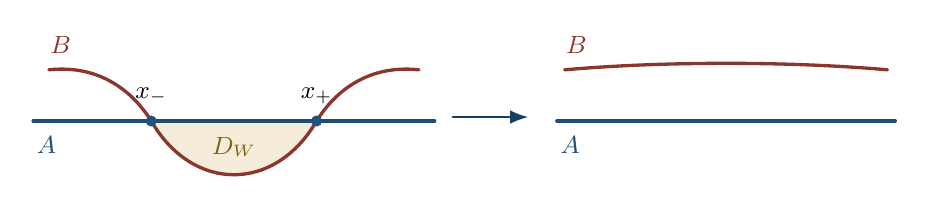
\begin{tikzpicture}[>=Latex,font=\small,line cap=round,
 line join=round]
 \fill[manifoldgold!17]
   (-1.05,0) .. controls (-.52,-.91) and (.52,-.91)
       .. (1.05,0) -- cycle;
 \draw[manifoldgold!75!black,densely dashed,thick]
   (-1.05,0) .. controls (-.52,-.91) and (.52,-.91)
       .. (1.05,0);
 \draw[manifoldblue!85!black,very thick] (-2.55,0)--(2.55,0);
 \draw[manifoldred!82!black,very thick]
   (-2.35,.65) .. controls (-1.70,.72) and (-1.28,.37)
       .. (-1.05,0) .. controls (-.52,-.91) and (.52,-.91)
       .. (1.05,0) .. controls (1.28,.37) and (1.70,.72)
       .. (2.35,.65);
 \fill[manifoldblue!90!black]
   (-1.05,0) circle (2pt) (1.05,0) circle (2pt);
 \node[above] at (-1.05,.10) {$x_-$};
 \node[above] at (1.05,.10) {$x_+$};
 \node[manifoldblue!85!black] at (-2.38,-.30) {$A$};
 \node[manifoldred!82!black] at (-2.20,.96) {$B$};
 \node[manifoldgold!65!black] at (0,-.33) {$D_W$};
 \draw[->,thick,manifoldblue!70!black] (2.78,.05)--(3.74,.05);
 \begin{scope}[shift={(6.25,0)}]
  \draw[manifoldblue!85!black,very thick] (-2.15,0)--(2.15,0);
  \draw[manifoldred!82!black,very thick]
    (-2.05,.65) .. controls (-.80,.76) and (.80,.76)
      .. (2.05,.65);
  \node[manifoldblue!85!black] at (-1.98,-.30) {$A$};
  \node[manifoldred!82!black] at (-1.90,.96) {$B$};
 \end{scope}
\end{tikzpicture}
\caption{Przekrój schematyczny ruchu Whitneya.
Po lewej łuki na $A$ i $B$ ograniczają jasny dysk,
a $x_-$ i $x_+$ mają przeciwne znaki. Po ruchu
przecięć nie ma. Rysunek pokazuje tylko przekrój;
w wyższych wymiarach niezbędne jest obramowanie
całego dysku.}
\label{fig:Whitney-chirurgia-21}
\end{figure}

Istnienie dysku z założeń stwierdzenia jest
\emph{osobną kwestią}. Okrąg $a\cup b$ musi być
nullhomotopijny; nawet wtedy dysk początkowo
może przecinać płaty lub mieć złe obramowanie.
Jeśli $\pi_1(N)\ne1$, dwa punkty o przeciwnych
znakach mogą mieć różne etykiety dróg $g,h$,
więc dają $g-h\ne0$ w $\Z[\pi_1(N)]$.
W wymiarze środkowym $n=2k$, $k\geq3$,
pełne kryterium zamiany obramowanej immersji
$S^k\looparrowright N^{2k}$ na zanurzenie
wyraża kwadratowe samoprzecięcie $\mu$;
to \href{https://webhomes.maths.ed.ac.uk/~v1ranick/books/scm.pdf}
{twierdzenie 5.2 Walla}, a nie wniosek
z samego rysunku. Dla $k=2$ kryterium to
może zawodzić. Tak właśnie powstaje granica
między chirurgią wysokowymiarową a wymiarem $4$.

\begin{stwierdzenie}[Forma na jądrze w wymiarze parzystym]
\label{prop:forma-jadra-21}
Niech $n=2k$, a $f:M^{2k}\to X^{2k}$ ma stopień
jeden. Forma przecięć na środkowej homologii
$H_k(M;\Z)/\mathrm{tors}$ rozkłada się ortogonalnie
na obraz $f_!$ oraz $K_k(f)/\mathrm{tors}$.
Forma na jądrze jest niezdegenerowana
(nad $\Z$: unimodularna na częściach wolnych).
Dla parzystego $k$ jest symetryczna, a dla
nieparzystego antysymetryczna.
\end{stwierdzenie}
\begin{proof}
Na częściach wolnych dualność Poincarégo
identyfikuje formę przecięć z iloczynem kubkowym:
$\lambda_M(x,y)=\langle\operatorname{PD}_M^{-1}x
\smile\operatorname{PD}_M^{-1}y,[M]\rangle$.
Dla $a,b\in H_k(X)$ z naturalności i warunku
$f_*[M]=[X]$ dostajemy
\[
 \lambda_M(f_!a,f_!b)
 =\langle f^*\operatorname{PD}_X^{-1}a
 \smile f^*\operatorname{PD}_X^{-1}b,[M]\rangle
 =\lambda_X(a,b).
\]
Dla $z\in K_k(f)$ oraz $a\in H_k(X)$,
naturalność iloczynu z klasą fundamentalną
i definicja $f_!$ dają
$\lambda_M(z,f_!a)=\lambda_X(f_*z,a)=0$.
Lemat~\ref{lem:split-normalne-21} daje rozkład
$H_k(M)=f_!H_k(X)\oplus K_k(f)$, więc jest
on ortogonalny. Na częściach wolnych forma
całej zamkniętej zorientowanej rozmaitości
jest unimodularna; podobnie forma na $X$.
Jeżeli w bazach dostosowanych do rozkładu
macierz jest blokowo diagonalna, a wyznaczniki
całości i bloku $X$ wynoszą $\pm1$, to także
wyznacznik bloku jądra wynosi $\pm1$.
Znak zamiany argumentów wynika z
$\alpha\smile\beta=(-1)^{k^2}\beta\smile\alpha$.
\end{proof}

\begin{przyklad}[Dwie sfery i ich jedno przecięcie]
\label{prz:forma-produkt-21}
Dla $M=S^k\times S^k$, $X=S^{2k}$, $k\geq3$,
weźmy mapę stopnia jeden z
Przykładu~\ref{prz:normalna-sfera-21}
(w tym kierunku wystarczy mapa zgniatająca).
Wtedy $K_k(f)=H_k(M)\cong\Z^2$,
generowane przez
$A=S^k\times\{*\}$ i $B=\{*\}\times S^k$.
Obie sfery mają trywialne wiązki normalne.
Możemy je przesunąć od samych siebie, zatem
$A\cdot A=B\cdot B=0$, ale $A$ i $B$
przecinają się w jednym punkcie.
W bazie $(A,B)$ otrzymujemy
\[
 \lambda=\begin{pmatrix}0&1\\(-1)^k&0\end{pmatrix}.
\]
Gdy $k$ jest parzyste, forma jest symetryczna;
gdy nieparzyste, antysymetryczna.
Nie wystarczy osobno policzyć, że obie sfery
reprezentują klasy jądra: ich wzajemne
przecięcie kontroluje możliwość kolejnych
operacji. W bardziej ogólnych sytuacjach
potrzebna jest ponadto informacja o
samoprzecięciach i obramowaniach, prowadząca
do form kwadratowych teorii chirurgii.
\end{przyklad}

\begin{uwaga}[Dwie różne przeszkody]
Grupy $L_n(\Z[\pi])$ opisują przeszkody
\emph{wykonania} dalszej chirurgii na mapie
normalnej, szczególnie w wymiarze środkowym.
Torsja Whiteheada w
$\operatorname{Wh}(\pi)$, poznana w
Rozdziale~\ref{ch:s-kobordyzm}, kontroluje
\emph{prostotę} otrzymanej równoważności
i iloczynowość $h$-kobordyzmu.
Są to różne etapy argumentu. Także późniejszy
ciąg dokładny chirurgii będzie wymagał
rozróżnienia zwykłych i prostych
równoważności homotopijnych.
\end{uwaga}

\section{Co pozostaje do zrobienia w programie chirurgii}
\label{sec:plan-chirurgia-21}

Dotychczasowe kroki można streścić bez
ukrywania danych potrzebnych dalej:
\begin{enumerate}[label=(\arabic*)]
\item Zaczynamy od odwzorowania normalnego
stopnia jeden $(f,b):M^n\to X^n$.
\item Wybieramy obramowane sfery reprezentujące
klasy jądra i wykonujemy chirurgię nad $X$,
pozostając w tej samej klasie normalnej kobordancji.
\item Sprawdzamy grupę podstawową i homologiczny
kompleks jądra nad $\Z[\pi_1(X)]$.
W wymiarze środkowym samo znikanie zwykłych
homologii już nie wystarcza: decydują formy
przecięć i ich kwadratowe uzupełnienia.
\item Po usunięciu tej przeszkody otrzymujemy
równoważność homotopijną; do klasyfikacji
rozmaitości trzeba jeszcze zrozumieć
jej torsję oraz klasę odpowiedniego
kobordyzmu.
\end{enumerate}

Następny rozdział zdefiniuje grupy chirurgiczne
$L_n(\Z[\pi])$ w odpowiednich wersjach,
pokaże proste przykłady form i sformułuje
twierdzenie o przeszkodzie chirurgicznej.
Później zbierzemy dane w ciągu dokładnym
chirurgii i zastosujemy je do klasyfikacji
rozmaitości.

\par\smallskip
{\footnotesize\noindent\emph{Dalsza lektura:}
\href{https://link.springer.com/chapter/10.1007/978-3-031-56334-8_4}
{W.~Lück i T.~Macko, \emph{The Surgery Step and $\xi$-Bordism}},
\href{https://webhomes.maths.ed.ac.uk/~v1ranick/books/scm.pdf}
{C.~T.~C. Wall, \emph{Surgery on Compact Manifolds}, §1--3}.\par}

\chapter{Formy kwadratowe i przeszkoda chirurgiczna}
\label{ch:przeszkoda-chirurgiczna}
\index{grupa L@Grupa $L$}

W Rozdziale~\ref{ch:chirurgia-geometryczna-21} operacja na
obramowanej sferze zmieniała rozmaitość, a forma przecięć
na jądrze mapy stopnia jeden pokazywała, dlaczego w
\emph{środkowym wymiarze} nie można usuwać klas po jednej.
Teraz zapiszemy to ograniczenie algebraicznie. Otrzymamy
grupę, w której klasa zerowa oznacza możliwość dokończenia
chirurgii przy odpowiednich założeniach wymiarowych.
Odróżnimy twierdzenia o konkretnych macierzach, które
udowodnimy tutaj, od głębokiego twierdzenia chirurgicznego
Walla, którego geometryczne lematy przywołamy jawnie.

\section{Drogi przecięcia i pierścień grupowy}
\label{sec:pi-formy-22}

Jeśli $X$ jest spójna, połóżmy $\pi=\pi_1(X)$ i
$\Lambda=\Z[\pi]$. Element $\Lambda$ jest skończoną
sumą $\sum_g n_g g$, gdzie $n_g\in\Z$. Mnożenie
przedłuża liniowo mnożenie w $\pi$. W przypadku
$\pi=1$ otrzymujemy zwykły pierścień $\Z$.
Niech $w:\pi\to\{\pm1\}$ będzie charakterem
orientacji celu. Na $\Lambda$ wprowadzamy \emph{inwolucję}
\begin{equation}\label{eq:inwolucja-L-22}
 \overline{\sum_g n_g g}
     =\sum_g n_g w(g)g^{-1}.
\end{equation}
Odwrócenie drogi zamienia $g$ na $g^{-1}$, a
$w(g)$ mówi, czy przeniesienie lokalnej orientacji
wzdłuż tej drogi zmienia znak.

\begin{stwierdzenie}[Dlaczego to inwolucja]
\label{prop:inwolucja-L-22}
Przepis~\eqref{eq:inwolucja-L-22} spełnia
$\overline{ab}=\bar b\bar a$ i
$\overline{\bar a}=a$.
\end{stwierdzenie}
\begin{proof}
Wystarczy sprawdzić elementy grupy, ponieważ obie
strony są addytywne. Ponieważ $w$ jest homomorfizmem,
\[
 \overline{gh}=w(g)w(h)h^{-1}g^{-1}
              =(w(h)h^{-1})(w(g)g^{-1})
              =\bar h\bar g.
\]
Ponadto $w(g^{-1})=w(g)$ i $w(g)^2=1$, skąd
$\overline{\bar g}=g$. Przedłużenie liniowe kończy
rachunek.
\end{proof}

Po podniesieniu sfer do nakrycia uniwersalnego
pojedynczy punkt ich przecięcia wnosi do
\emph{współczynnika przecięcia} znak razy element $g\in\pi$.
Znak zależy od orientacji, a $g$ od obranych dróg
od punktu bazowego do sfer. Dlatego dwa przecięcia
o przeciwnych znakach mogą sumować się do
$g-h\ne0$ w $\Lambda$, choć ich zwykła liczba
przecięcia jest zerem. Zmiana dróg zmienia zapis
macierzy, lecz nie jej klasę izometrii.

\begin{definicja}[Forma $\epsilon$-hermitowska]
\label{def:hermitowska-22}
Niech $P$ będzie skończenie generowanym rzutowym
lewym modułem
nad $\Lambda$ oraz $\epsilon\in\{\pm1\}$.
\emph{Formą $\epsilon$-hermitowską} nazywamy
odwzorowanie $\lambda:P\times P\to\Lambda$
addytywne w każdej zmiennej i takie, że
\[
 \lambda(ax,by)=a\lambda(x,y)\bar b,\qquad
 \lambda(y,x)=\epsilon\overline{\lambda(x,y)}.
\]
Jest \emph{nieosobliwa}, gdy odwzorowanie
$P\to P^*$, $y\mapsto\lambda(-,y)$, jest
izomorfizmem. Tutaj
$P^*=\operatorname{Hom}_\Lambda(P,\Lambda)$
jest lewym modułem z działaniem
$(a\cdot h)(x)=h(x)\bar a$; dzięki temu
$y\mapsto\lambda(-,y)$ jest liniowe.
\end{definicja}

Dla $n=2k$ przecięcia $k$-wymiarowych sfer
spełniają ten wzór z $\epsilon=(-1)^k$:
zamiana kolejności dwóch przestrzeni stycznych
w punkcie przecięcia zamienia bloki po $k$ wektorów,
co daje znak $(-1)^{k^2}=(-1)^k$; odwraca także
drogę, stąd kreska nad współczynnikiem.

\section{Samoprzecięcia i formy kwadratowe}
\label{sec:kwadratowa-22}

Sama $\lambda$ nie zapamiętuje, czy reprezentant
klasy daje się przedstawić jako \emph{obramowana,
zanurzona} sfera. Potrzebna jest poprawka
samoprzecięciowa $\mu$; jej precyzyjną postać
podajemy w języku algebraicznym. Dla
$\epsilon=(-1)^k$ oznaczmy
\[
 Q_\epsilon(\Lambda)=
 \Lambda/\{a-\epsilon\bar a:a\in\Lambda\}.
\]
W mianowniku chodzi o podgrupę addytywną, a nie
zwykle o ideał. Nawias $[a]$ oznacza klasę $a$.

\begin{definicja}[Forma $\epsilon$-kwadratowa]
\label{def:forma-kwadratowa-22}
To para $(\lambda,\mu)$ na $P$, gdzie $\lambda$
jest nieosobliwą formą $\epsilon$-hermitowską, a
$\mu:P\to Q_\epsilon(\Lambda)$ spełnia
\begin{align}
 \mu(x+y)&=\mu(x)+\mu(y)+[\lambda(x,y)],
                   \label{eq:quad-add-22}\\
 \mu(ax)&=[a m\bar a]\quad\text{dla }m\in\mu(x),
                                                \label{eq:quad-scal-22}\\
 \lambda(x,x)&=a+\epsilon\bar a
       \quad\text{dla dowolnego }a\in\mu(x).
                   \label{eq:quad-diag-22}
\end{align}
Drugi wzór jest niezależny od wyboru $m$:
$a(c-\epsilon\bar c)\bar a$ ma postać
$d-\epsilon\bar d$ dla $d=ac\bar a$.
Ostatni wzór jest niezależny od reprezentanta
$a$: dodanie $c-\epsilon\bar c$ nie zmienia
$a+\epsilon\bar a$.
\end{definicja}

Geometrycznie $\mu(x)$ liczy samoprzecięcia
obramowanej immersji sfery i uwzględnia obramowanie.
Równanie~\eqref{eq:quad-add-22} mówi:
gdy połączymy reprezentantów $x$ i $y$, nowe
samoprzecięcia obejmują też przecięcia obu sfer.
W \eqref{eq:quad-diag-22} widać, dlaczego
„połowa przekątnej” nie zawsze wystarcza:
nad $\Z[\pi]$ nie można po prostu dzielić przez $2$.

\begin{stwierdzenie}[Rachunek przecięć na nakryciu]
\label{prop:rachunek-przeciec-Wall-22}
Niech $k\geq3$, a $M^{2k}\to X^{2k}$ będzie
$k$-spójnym odwzorowaniem normalnym stopnia jeden.
Wybierzmy obramowane, poprzeczne immersje
$k$-sfer reprezentujące $x,y\in K_k(M)$,
wraz z drogami od punktu bazowego. Każdy punkt
$p$ przecięcia wnosi znak $\varepsilon_p$ i element
$g_p\in\pi_1(X)$, wyznaczony przez przejście
między wybranymi podniesieniami sfer. Wtedy
\[
 \lambda(x,y)=\sum_{p\in x\pitchfork y}
                  \varepsilon_p g_p\in\Lambda.
\]
Wybierając przy każdym podwójnym punkcie immersji
$x$ jedną z dwóch kolejności gałęzi, otrzymujemy
\[
 \mu(x)=\left[\sum_{p\in\operatorname{Dbl}(x)}
                 \varepsilon_p g_p\right]
                 \in Q_{(-1)^k}(\Lambda).
\]
Wartości te nie zależą od regularnej homotopii
reprezentantów; spełniają
\eqref{eq:quad-add-22} i~\eqref{eq:quad-diag-22}.
\end{stwierdzenie}
\begin{proof}
Podnieśmy obie sfery do nakrycia uniwersalnego.
Współczynnik przy $g$ w $\lambda(x,y)$ jest
zwykłą algebraiczną liczbą przecięć jednego
podniesienia z przesunięciem drugiego przez $g$.
Jest więc stały przy homotopii. Po zamianie
obu sfer droga odwraca się, a znak zmienia się
o $(-1)^k w(g)$. To daje hermitowskość z
Definicji~\ref{def:hermitowska-22}.

Przy podwójnym punkcie zamiana kolejności
gałęzi zmienia $\varepsilon_p g_p$ na
$(-1)^k\overline{\varepsilon_p g_p}$.
Oba wyrazy mają tę samą klasę w
$Q_{(-1)^k}(\Lambda)$. Podczas ogólnej regularnej
homotopii punkty podwójne rodzą się lub znikają
parami o przeciwnych znakach i tej samej
etykiecie, zatem $\mu$ się nie zmienia.
Po połączeniu dwóch sfer rurką nowe punkty
podwójne to, oprócz dawnych, dokładnie ich
wzajemne przecięcia. Dostajemy stąd
\eqref{eq:quad-add-22}.

Na koniec odsuńmy immersję reprezentującą $x$
wzdłuż jej obramowania. Przy każdym podwójnym
punkcie odsunięta sfera przecina pierwotną
dwukrotnie, raz dla każdej kolejności gałęzi.
Ich suma wynosi $a+(-1)^k\bar a$ dla składnika
$a$ w $\mu(x)$. Wkład przekątnej z klasy Eulera
wiązki normalnej znika, bo sfera jest obramowana.
To jest~\eqref{eq:quad-diag-22}.
\end{proof}

Rachunek punktów wyjaśnia wzory, lecz aby
traktować $\mu$ jako funkcję na $K_k(M)$,
trzeba jeszcze wiedzieć, że dane normalne
wyznaczają właściwą klasę regularnej homotopii
obramowanych immersji. To identyfikacja
użyta w twierdzeniu 5.2 Walla; nie wynika
z samego zliczenia punktów.

Na przykład dwa przecięcia o znakach $+1$ i $-1$
oraz etykietach $1$ i $t$ dają
$\lambda(x,y)=1-t\in\Z[t,t^{-1}]$ dla
$\pi_1(X)=\langle t\rangle$. Zwykła liczba
przecięcia jest zerem, lecz okrąg złożony z
łuków obu sfer reprezentuje $t$ lub $t^{-1}$
i nie ogranicza
dysku Whitneya. Dopiero przeciwne znaki z
\emph{jednakową} etykietą pozwalają szukać
takiego dysku. Warunek $\mu(x)=0$ dopuszcza
analogiczne sparowanie samoprzecięć. Wyjaśnijmy
osobno, dlaczego w wymiarach co najmniej sześć
takie pary można usunąć.

\subsection*{Od samoprzecięć do zanurzonej sfery}
\index{trik Whitneya@Trik Whitneya!samoprzecięcia}
W tym kroku potrzebna jest \emph{obramowana
immersja}, a nie jedynie ciągłe odwzorowanie
$S^k\to M$. Obramowanie jest częścią klasy
regularnej homotopii wyznaczonej przez mapę
normalną i wypełnienie obrazu sfery w $X$.

\begin{stwierdzenie}[Kryterium zanurzania Walla w środku wymiaru]
\label{prop:osadzenie-Wall-52-22}
Niech $k\geq3$, a $M^{2k}$ będzie spójną gładką
rozmaitością. Niech $u:S^k\times D^k\looparrowright
\operatorname{int}M$ będzie obramowaną immersją,
której rdzeń ma jedynie poprzeczne punkty podwójne.
Oznaczmy $\pi=\pi_1(M)$ i wybierzmy drogi bazowe
potrzebne do określenia
$\mu(u)\in Q_{(-1)^k}(\Z[\pi])$.
Jeśli $\mu(u)=0$, to $u$ jest regularnie homotopijna
do immersji, której rdzeń jest zanurzony. Po
zwężeniu włókien $D^k$ otrzymujemy zanurzenie
$S^k\times D^k\hookrightarrow M$ w tej samej
klasie regularnej homotopii. Dla zanurzonego rdzenia
warunek $\mu(u)=0$ jest konieczny.
\end{stwierdzenie}
\begin{proof}[Dowód z obramowanym trikiem Whitneya]
\textbf{1. Parowanie punktów.}
Niech $\epsilon=(-1)^k$. W grupie
$Q_\epsilon(\Z[\pi])$ zamiana kolejności dwóch
gałęzi w punkcie o etykiecie $g$ zamienia składnik
$\varepsilon g$ na $\epsilon\overline{\varepsilon g}
=\epsilon w(g)\varepsilon g^{-1}$.
Rozłóżmy bazę grupy pierścienia na orbity
$g\leftrightarrow g^{-1}$. Dla orbity dwuelementowej
możemy więc wszystkie składniki zapisać przy tej
samej etykiecie $g$; ich suma całkowita jest zerowa.
Dla orbity jednoelementowej $g=g^{-1}$ otrzymujemy
albo kopię $\Z$, albo $\Z/2$, zależnie od znaku
$\epsilon w(g)$. W pierwszym przypadku suma znaków
jest zerowa. W drugim liczba punktów jest parzysta,
a zamiana gałęzi zmienia ich znaki. W każdym
przypadku punkty dają się zatem podzielić na pary
$(p,q)$ o \emph{jednakowej} etykiecie i przeciwnych
znakach, po odpowiednim wyborze kolejności gałęzi.

\textbf{2. Okrąg Whitneya.}
W dziedzinie $S^k$ wybierzmy od $p$ do $q$ jeden
łuk na pierwszym płacie, a drugi na drugim.
Ponieważ $k\geq3$, łuki można wybrać rozłączne
poza końcami i ominąć preobrazy pozostałych
punktów podwójnych. Ich obrazy tworzą okrąg
Whitneya. Przy ustalonych drogach bazowych jego
klasa w $\pi_1(M)$ jest, z dokładnością do
odwrócenia i sprzężenia, iloczynem $g_p g_q^{-1}$.
Równość etykiet daje więc pętlę homotopijnie
trywialną. Ten krok nie wymaga $\pi_1(M)=1$;
właśnie temu służą etykiety w $\Z[\pi]$.

\textbf{3. Czysty dysk.}
Odsuńmy okrąg od obu lokalnych płatów. Inkluzja
$M\setminus u(S^k\times\{0\})\hookrightarrow M$
indukuje izomorfizm na $\pi_1$: pętle i homotopie
reprezentowane przez dwuwymiarowe dyski można
przesunąć poza obraz sfery, gdyż
$2+k<2k$ dla $k\geq3$. Skończony zbiór punktów
podwójnych nie zmienia tego rachunku. Odsunięty
okrąg ogranicza więc dysk w dopełnieniu.
Transwersalność względna pozwala wybrać dysk
gładki, z wnętrzem rozłącznym z obrazem rdzenia;
nierówność $2+2<2k$ pozwala usunąć także jego
samoprzecięcia. Dołączając kołnierz przy łukach,
otrzymujemy zanurzony dysk Whitneya $D_W$ o brzegu
na dwóch wybranych płatach.

\textbf{4. Obramowanie i ruch.}
Sam czysty dysk nie wystarcza do ruchu z
Stwierdzenia~\ref{prop:lokalny-Whitney-21}.
Wzdłuż pierwszego łuku wybieramy $(k-1)$ kierunków
stycznych do płata i prostopadłych do łuku;
w punktach końcowych poprzeczność identyfikuje
je z kierunkami normalnymi do drugiego płata.
Ponieważ okrąg Whitneya jest zerowy w $\pi_1(M)$,
możemy spójnie przenosić orientację $M$ wzdłuż
jego brzegu także wtedy, gdy całe $M$ nie jest
orientowalne. Przeciwne znaki w $p$ i $q$ sprawiają,
że po odwróceniu kierunku drugiego łuku orientacje
ram końcowych są zgodne. Przestrzeń pośrednich
zorientowanych ram jest spójna, bo $SO(k-1)$
jest spójna dla $k\geq3$; wybieramy więc ramę
normalną do drugiego płata na całym drugim łuku.
Obie części sklejają się w $(k-1)$-ramę na
$\partial D_W$. Wiązka normalna
dysku ma rangę $2k-2$ i jest trywialna. Przeszkodę
przedłużenia powyższej $(k-1)$-ramy mierzy
$\pi_1(V_{2k-2,k-1})$, która jest zerowa dla
$k\geq3$. Pozostałe kierunki uzupełniamy nad
dyskiem. Otrzymujemy lokalne otoczenie modelowe
$D^2\times D^{k-1}\times D^{k-1}$, w którym
dwa płaty zajmują dwa prostopadłe układy pasów.
Precyzyjna konstrukcja tego otoczenia jest
obramowanym trikiem Whitneya: używamy
\href{https://webhomes.maths.ed.ac.uk/~v1ranick/surgery/hcobord.pdf}
{Milnora, twierdzenia 6.6 i lematów 6.7 oraz 6.13}.
W naszym zastosowaniu oba płaty mają wymiar $k$
w otoczeniu wymiaru $2k$. Warunki wymiarowe
Milnora sprowadzają się więc do $k\geq3$.
Osobno potrzebujemy ściągalności okręgu Whitneya;
jego łuki wybieramy tak, by omijały pozostałe
przecięcia. Lematy 6.7
i 6.13 dostarczają właśnie produktowego modelu
otoczenia dysku oraz zgodnych ram normalnych.
Twierdzenie 6.6 Milnora jest sformułowane dla
dwóch zanurzonych podrozmaitości; zastosowanie
modelu do dwóch lokalnych płatów jednej immersji
wymaga jeszcze argumentu Walla z twierdzenia 5.2.
Przed tym krokiem można zwęzić włókna $D^k$,
aby otoczenie dysku było wolne od pozostałych
części pogrubionej immersji.
Lokalny ruch z
Stwierdzenia~\ref{prop:lokalny-Whitney-21}
usuwa teraz $p$ i $q$. Dla jednej samoprzecinającej
się sfery ograniczamy uwagę do dwóch zanurzonych
fragmentów odpowiadających wybranym łukom
i wykonujemy go na jednym \emph{lokalnym płacie};
jest to regularna homotopia
immersji, nie izotopia otaczająca całego $M$.
Jej podparcie omija pozostałe punkty podwójne.
Przejście od twierdzenia Milnora o dwóch zanurzonych
podrozmaitościach do dwóch płatów jednej immersji
jest geometryczną częścią kryterium~5.2 Walla.
Powtarzamy krok dla wszystkich par.

Regularna homotopia przenosi obramowanie i klasę
normalną. Gdy rdzeń jest już zanurzony, zwężamy
włókna $D^k$ w obramowanym otoczeniu; zwartość
$S^k$ zapewnia, że dla dostatecznie małego promienia
całe pogrubienie jest zanurzone. Zanurzony rdzeń
nie ma punktów podwójnych, więc jego $\mu$ wynosi
zero.
\end{proof}

Przy zastosowaniu do $x\in K_k(M)$ potrzebne są
jeszcze dwa wejścia. Po przygotowaniu
$k$-spójnej mapy normalnej $M\to X$ mamy
$\pi_1(M)\cong\pi_1(X)$ oraz
$K_k(M)\cong\pi_{k+1}(f)$; wybór właściwej
obramowanej klasy regularnej homotopii immersji
$S^k\times D^k$ jest treścią
\href{https://webhomes.maths.ed.ac.uk/~v1ranick/books/scm.pdf}
{Walla, twierdzenia 1.1}. Przytoczona konstrukcja
produktowego otoczenia dysku pozostaje osobnym
lematem geometrycznym Milnora; powyższy rachunek
nie jest samodzielnym dowodem tego lematu.
W wymiarze cztery nierówności z kroku 3 zawodzą,
więc sam warunek $\mu=0$ nie daje analogicznego
wniosku. Ponadto uogólnienie $\lambda,\mu$ z
uwagi 5.2.1 Walla na nakrycie indukowane z innej
rozmaitości nie obejmuje kryterium zanurzania.

\begin{przyklad}[Co zostaje, gdy $\pi=1$]
\label{prz:mu-Z-22}
Dla $\Lambda=\Z$ inwolucja jest zwykłą tożsamością.
Jeśli $k$ jest parzyste, $Q_+(\Z)=\Z$,
a~\eqref{eq:quad-diag-22} daje
$\lambda(x,x)=2\mu(x)$. Forma jest więc
\emph{parzysta}; $\mu(x)=\lambda(x,x)/2$.
Jeśli $k$ jest nieparzyste,
$Q_-(\Z)=\Z/2$; forma $\lambda$ jest
antysymetryczna i $\lambda(x,x)=0$,
ale $\mu(x)\in\Z/2$ może być niezerowe.
Ta ostatnia informacja nie daje się odczytać
z samej macierzy przecięć.
\end{przyklad}

\begin{definicja}[Para hiperboliczna i lagranżjan]
\index{para hiperboliczna i lagranzjan@Para hiperboliczna i lagranżjan}
\label{def:hiperboliczna-22}
Wolny moduł o bazie $(e_1,f_1,\dots,e_r,f_r)$
z macierzą w każdej parze
\[
 H_\epsilon=
 \begin{pmatrix}0&1\\\epsilon&0\end{pmatrix},
 \qquad \mu(e_i)=\mu(f_i)=0,
\]
oraz z zerowymi sprzężeniami między różnymi
parami, nazywamy \emph{hiperbolicznym}.
\emph{Lagranżjanem} formy kwadratowej jest
bezpośredni składnik $L\subset P$ taki, że
$L=L^\perp$ oraz $\mu|_L=0$.
W parze hiperbolicznej
$L=\langle e_1,\dots,e_r\rangle$ jest lagranżjanem.
\end{definicja}

Parę o macierzy $H_\epsilon$ realizują klasy
dwóch sfer czynnikowych w $S^k\times S^k$,
jak w Przykładzie~\ref{prz:forma-produkt-21}.
Lokalny model ich jednego przecięcia
pokazuje Rysunek~\ref{fig:para-hiperboliczna-22}.

\begin{figure}[htbp]
\centering
\begin{tikzpicture}[>=Latex,font=\small,line cap=round]
 \fill[manifoldblue!12,rounded corners=4pt]
   (-3.15,-.20) rectangle (3.15,.20);
 \fill[manifoldgold!19,rounded corners=4pt]
   (-.20,-1.12) rectangle (.20,1.12);
 \draw[manifoldblue!80!black,very thick]
   (-3.15,0)--(3.15,0);
 \draw[manifoldgold!85!black,very thick]
   (0,-1.12)--(0,1.12);
 \fill[manifoldred!85!black] (0,0) circle (2.5pt);
 \node[manifoldblue!80!black,anchor=west]
   at (-3.15,-.65) {$D^k\times\{0\}$};
 \node[manifoldgold!75!black,anchor=west]
   at (.38,.88) {$\{0\}\times D^k$};
 \node[manifoldred!85!black,anchor=west]
   at (.32,-.43) {jedno przecięcie};
\end{tikzpicture}
\caption{Lokalny model sfer
$e=S^k\times\{*\}$ i $f=\{*\}\times S^k$.
Ich dyski współrzędnych przecinają się
tylko w środku; po uzgodnieniu orientacji
$\lambda(e,f)=1$. Każda sfera ma
trywialną wiązkę normalną, więc
$\mu(e)=\mu(f)=0$. Jasne pasy pokazują
jedynie przekrój otoczeń, a nie całe sfery.}
\label{fig:para-hiperboliczna-22}
\end{figure}

\subsection*{Przesunięcie uchwytu jako zmiana bazy}
Stwierdzenie~\ref{prop:slide-18} opisało geometryczny
ruch dwóch uchwytów tego samego indeksu:
$e_i$ zostaje zastąpione przez $e_i\pm e_j$.
W wymiarze środkowym wpływ tego ruchu na
rachunek przecięć można wypisać bez kolejnego
twierdzenia geometrycznego. Jeżeli kolumny
macierzy $P$ wyrażają nową bazę w starej,
to macierz formy w nowej bazie wynosi
\begin{equation}\label{eq:slide-forma-22}
 A'=P^{T}AP,\qquad
 \mu(e_i\pm e_j)
   =\mu(e_i)+\mu(e_j)
      \pm[\lambda(e_i,e_j)].
\end{equation}
Pierwsza równość pochodzi z dwuliniowości
$\lambda$ nad $\Z$; druga z
\eqref{eq:quad-add-22} i
$\mu(-e_j)=\mu(e_j)$.
Na przykład dla symetrycznej pary hiperbolicznej
$A=\left(\begin{smallmatrix}0&1\\1&0\end{smallmatrix}\right)$
przesunięcie $e'=e+f$ daje
\[
 A'=\begin{pmatrix}2&1\\1&0\end{pmatrix},
 \qquad \mu(e')=1.
\]
Pojawienie się niezerowego wyrazu na przekątnej
nie tworzy nowej przeszkody: zmieniła się baza
tej samej formy. Przy niebanalnej $\pi_1$ w
\eqref{eq:slide-forma-22} trzeba zastąpić
transpozycję transpozycją sprzężoną oraz
śledzić etykiety dróg; sama macierz całkowita
nie zawiera wtedy całej informacji.

Wypiszmy taką zmianę bazy nad
$\Lambda=\Z[\pi]$ z inwolucją
\eqref{eq:inwolucja-L-22}. W sumie dwóch
płaszczyzn hiperbolicznych połóżmy, dla
dowolnego $a\in\Lambda$,
\[
 e'_1=e_1+a e_2,\qquad e'_2=e_2,\qquad
 f'_1=f_1,\qquad f'_2=f_2-\bar a f_1.
\]
Współczynnik $\bar a$ jest konieczny:
seskwiliniowość daje
\[
 \lambda(e'_1,f'_2)
 =\lambda(ae_2,f_2)-\lambda(e_1,\bar a f_1)
 =a-\overline{\bar a}=0.
\]
Pozostałe mieszane parowania nadal wynoszą
$\lambda(e'_i,f'_j)=\delta_{ij}$; parowania
wewnątrz rodzin $e'$ i $f'$ są zerowe.
Z~\eqref{eq:quad-add-22} wynika również
$\mu(e'_i)=\mu(f'_i)=0$, bo składniki dodawane
do siebie należą do wzajemnie ortogonalnych
lagranżjanów. Zatem nowa baza jest znowu
hiperboliczna. Na $\langle e_1,e_2\rangle$
zmianę opisuje macierz elementarna z
współczynnikiem $a$, a na dualnej rodzinie
odwrotna zmiana sprzężona ze współczynnikiem
$-\bar a$. Obie mają klasę zerową w
$\operatorname{Wh}(\pi)$
(Definicja~\ref{def:k1-wh-20}). Ruch nie zmienia
więc \emph{prostej} klasy bazy; sama równość
macierzy form bez tej kontroli nie dawałaby
takiego wniosku.

\begin{stwierdzenie}[Dlaczego hiperboliczna para nie przeszkadza]
\label{prop:hiperboliczna-22}
W parze $(e,f)$ mamy $\lambda(e,f)=1$,
$\lambda(e,e)=\lambda(f,f)=0$ oraz
$\mu(e)=\mu(f)=0$. Formy hiperboliczne
tworzą neutralne składniki przy stabilizacji.
Ich sygnatura, gdy $\epsilon=+1$ i $\Lambda=\Z$,
jest równa zeru.
\end{stwierdzenie}
\begin{proof}
Pierwsze równości odczytujemy z macierzy.
Na prostą generowaną przez $e$ forma
i funkcja kwadratowa znikają, a jej
ortogonalne dopełnienie wyznacza warunek
$\lambda(ae+bf,e)=\epsilon b=0$, więc
to znowu $\langle e\rangle$.
Dla $\epsilon=+1$ macierz ma wartości własne
$+1$ i $-1$, stąd jej sygnatura wynosi zero.
Suma wielu par ma lagranżjan będący sumą
odpowiednich prostych.
\end{proof}

\begin{figure}[htbp]
\centering
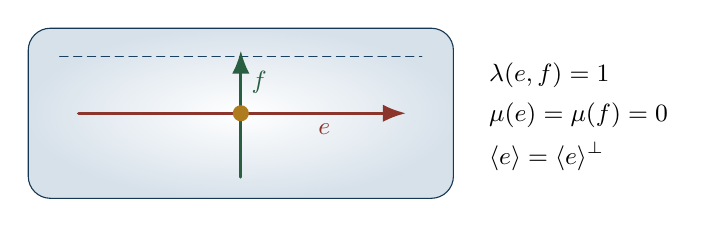
\begin{tikzpicture}[>=Latex,font=\small,line cap=round]
 \shade[inner color=white,outer color=manifoldblue!18,
        rounded corners=8pt] (-2.7,-1.08) rectangle (2.7,1.08);
 \draw[manifoldblue!60!black,rounded corners=8pt]
       (-2.7,-1.08) rectangle (2.7,1.08);
 \draw[manifoldblue!70!black,densely dashed]
       (-2.30,.72)--(2.30,.72);
 \draw[manifoldred!82!black,very thick,->]
       (-2.06,0)--(2.10,0)
       node[near end,below] {$e$};
 \draw[manifoldgreen!75!black,very thick,->]
       (0,-.81)--(0,.80)
       node[near end,right] {$f$};
 \fill[manifoldgold!85!black] (0,0) circle (2.9pt);
 \node[anchor=west] at (3.03,.48)
       {$\lambda(e,f)=1$};
 \node[anchor=west] at (3.03,-.03)
       {$\mu(e)=\mu(f)=0$};
 \node[anchor=west] at (3.03,-.55)
       {$\langle e\rangle=\langle e\rangle^\perp$};
\end{tikzpicture}
\caption{Lokalny schemat pary hiperbolicznej.
Sfery reprezentujące $e$ i $f$ spotykają się poprzecznie
w jednym punkcie, a każdą z nich osobno można
obramować bez samoprzecięć. Wybór kierunku $e$
wyznacza lagranżjan; prostokąt jest tylko fragmentem
otoczenia przecięcia, nie całą rozmaitością.}
\label{fig:hiperboliczna-22}
\end{figure}

\begin{przyklad}[Produkt sfer z poprzedniego rozdziału]
\label{prz:produkt-L-22}
W Przykładzie~\ref{prz:forma-produkt-21}
klasy $e=[S^k\times\{*\}]$ i
$f=[\{*\}\times S^k]$ mają macierz $H_{(-1)^k}$.
Dla standardowych danych normalnych lokalnej
stabilizacji z
Lematu~\ref{lem:wall-lokalna-stabilizacja-22}
obie sfery są obramowanymi reprezentantami
bez punktów podwójnych, więc
$\mu(e)=\mu(f)=0$. Samą macierz przecięć
trzeba uzupełnić o ten wybór obramowań;
Przykład~\ref{prz:Arf-dwie-22} pokazuje dlaczego.
To przykład jądra \emph{niezerowego jako moduł},
które daje \emph{zerową przeszkodę}:
można usunąć parę za pomocą odpowiednich chirurgii.
Dla $k=3$ jest to jądro mapy na górnym brzegu
śladu z Przykładu~\ref{prz:slad-s6-produkt-21}.
Jego miejsce w ciągu chirurgii opisuje
Przykład~\ref{prz:slad-s6-ciag-23}.
\end{przyklad}

\section{Co oznacza grupa \texorpdfstring{$L$}{L}}
\label{sec:grupy-L-22}

W wymiarze $2k$ sumujemy formy kwadratowe
ortogonalnie. Dwie formy uważa się za równoważne
w sensie Witta, jeśli ich ortogonalna różnica,
po ewentualnym dodaniu form hiperbolicznych,
ma lagranżjan. W wersji $L^s$ moduły mają
preferowane bazy stabilne, a dla lagranżjanu
$L\subset P$ odwzorowanie $P/L\to L^*$
wyznaczone przez $\lambda$ ma być \emph{prostym}
izomorfizmem względem tych baz. Jest to algebraiczny warunek
zerowania różnicy klas. Klasy z dodawaniem
przez sumę ortogonalną tworzą \emph{kwadratową grupę
chirurgiczną} $L_{2k}(\Lambda)$, z odpowiednią
dekoracją opisaną poniżej. Wersję opartą na bazach
i prostych równoważnościach oznaczymy
$L^s_{2k}(\Lambda,w)$. Warunek „prosta” dotyczy
również dualności formy: izomorfizm do modułu dualnego
ma zerową torsję w $\operatorname{Wh}(\pi)$.
Wersja $L^h_{2k}$ używa zwykłej równoważności
homotopijnej. Dla $\pi=1$ te rozróżnienia znikają.

\subsection*{Dekoracje $s$ i $h$ w rachunku baz}
\label{sec:dekoracje-L-22}
Intuicją dekoracji jest pytanie, jaki rodzaj
równoważności ma pozostać po usunięciu jądra:
$h$ oznacza równoważność homotopijną, a $s$
równoważność \emph{prostą}. W rozdziale o torsji
warunek prostoty zapisaliśmy jako znikanie klasy
macierzy w $\operatorname{Wh}(\pi)$
(Definicja~\ref{def:k1-wh-20}). Dla formy
na bazowanym wolnym module jej dualność
$P\to P^*$ musi być w wersji $s$ prostym
izomorfizmem. Przy usuwaniu lagranżjanu
trzeba ponadto sprawdzić prostotę
$P/L\to L^*$, co wykorzystaliśmy w
Lemacie~\ref{lem:lagr-hip-Z-22}.
W wersji $h$ wymagamy zwykłych izomorfizmów:
macierz odwracalna może mieć niezerową klasę
Whiteheada. To rozróżnienie i odpowiadające
mu grupy przeszkód opisuje
\href{https://webhomes.maths.ed.ac.uk/~v1ranick/books/scm.pdf}
{Wall, \emph{Surgery on Compact Manifolds}, §17D}.

\begin{przyklad}[Odwracalna dualność, która nie jest prosta]
\label{prz:dekoracje-C5-22}
Niech $\pi=C_5=\langle t\mid t^5=1\rangle$,
$w=1$, $\Lambda=\Z[C_5]$ oraz
$u=1-t-t^{-1}$. W
Przykładzie~\ref{prz:wh-c5-20} sprawdziliśmy,
że $u$ jest jednostką z odwrotnością
$v=1-t^2-t^{-2}$, ale $[u]\ne0$ w
$\operatorname{Wh}(C_5)$. Ponadto $\bar u=u$
i $\bar v=v$. Na $P=\Lambda e\oplus\Lambda f$
weźmy formę $+$-kwadratową określoną przez
\[
 \lambda(e,e)=\lambda(f,f)=0,\qquad
 \lambda(e,f)=\lambda(f,e)=u,\qquad
 \mu(e)=\mu(f)=0.
\]
Dla $x=ae+bf$ mamy
$\mu(x)=[a u\bar b]\in Q_+(\Lambda)$;
stąd $\lambda(x,x)$ jest sumą tego
reprezentanta i jego sprzężenia, zgodnie z
\eqref{eq:quad-diag-22}. Podstawienie
$f'=vf$ daje $\lambda(e,f')=u\bar v=1$
i $\mu(f')=0$, więc po zwykłej zmianie bazy
forma jest hiperboliczna.

W bazie $(e,f)$ macierz dualności ma postać
$\left(\begin{smallmatrix}0&u\\u&0\end{smallmatrix}\right)$.
Zamiana dwóch kolumn wnosi tylko znak,
który znika w grupie Whiteheada. Dlatego
torsja tej dualności wynosi
$[u]+[u]=2[u]\ne0$.
Ostatnią nierówność można sprawdzić tym
samym homomorfizmem co w
Przykładzie~\ref{prz:wh-c5-20}:
$|u(e^{2\pi i/5})|^2\ne1$.
Forma dopuszcza więc zwykłą dualność i
reprezentuje zero w opisie $h$, lecz z tą
preferowaną bazą nie spełnia warunku prostej
dualności potrzebnego do zdefiniowania jej
klasy w $L^s_{4j}(\Lambda,1)$.
Przykład dotyczy danych algebraicznych;
nie twierdzimy tu, że wybrana forma jest
jądrem określonej mapy normalnej.
\end{przyklad}

Gdy $\pi=1$, mamy
$\operatorname{Wh}(\pi)=0$
(Stwierdzenie~\ref{prop:wh-trywialna-20}),
więc powyższa różnica warunków znika.
Relatywna wersja twierdzenia o przeszkodzie
zachowuje to samo rozróżnienie na brzegu:
przy dekoracji $s$ zastana mapa brzegu jest
prostą równoważnością homotopijną, przy
dekoracji $h$ zwykłą równoważnością.

W nieparzystym wymiarze jądro nie jest opisywane
pojedynczą formą środkową. Model algebraiczny ma
postać \emph{formacji}: hiperboliczny moduł
kwadratowy wraz z dwoma lagranżjanami. Ich
przecięcie i iloraz przez ich sumę mierzą dwa
sąsiednie jądra mapy; wyprowadzimy to niżej.
Formacje dzielimy przez stabilizację i relację
wyznaczoną przez kobordyzm formacji; otrzymujemy
$L^s_{2k+1}(\Lambda,w)$ lub $L^h_{2k+1}(\Lambda,w)$.
W pełnej definicji obejmującej wszystkie wymiary
są to klasy kobordyzmu skończonych
\emph{kwadratowych kompleksów Poincarégo}
nad $\Lambda$. Konstrukcja formacji jest ich
nieparzystowym opisem po usunięciu homotopijnych
składników poniżej środka. Nie utożsamiamy
nieparzystej grupy z grupą Witta macierzy z poprzedniej sekcji.

\begin{uwaga}[Nie mylmy dwóch słów „torsja”]
W $\operatorname{Wh}(\pi)$ torsja oznacza torsję
\emph{równoważności łańcuchowej} z
Rozdziału~\ref{ch:s-kobordyzm}; w grupie $L$
klasyfikujemy formy i kwadratowe kompleksy.
To, że algebraiczne $K$- i $L$-teoria korzystają
z tych samych modułów nad $\Z[\pi]$, nie czyni
ich przeszkód tym samym obiektem.
\end{uwaga}

\section{Przypadek prostej spójności: sygnatura i Arf}
\label{sec:obliczenia-LZ-22}

Dla $\pi=1$ grupy kwadratowe w wysokowymiarowej
teorii chirurgii mają czterookresowy wzór
\begin{equation}\label{eq:L-Z-22}
 L_{4j}(\Z)\cong\Z,\qquad
 L_{4j+1}(\Z)=0,\qquad
 L_{4j+2}(\Z)\cong\Z/2,\qquad
 L_{4j+3}(\Z)=0.
\end{equation}
Wzór jest twierdzeniem klasyfikacyjnym teorii $L$;
poniżej wyjaśniamy jego dwa niezerowe inwarianty
i sprawdzamy konkretne formy. Nie wyprowadzamy
samych obliczeń grup nieparzystych z rachunku
dwóch macierzy: wymagałoby to teorii formacji.

\subsection*{Wymiary podzielne przez cztery}
Niech $n=4j$, $k=2j$. Środkowa forma jest
parzysta, symetryczna i unimodularna.
Jej \emph{sygnatura} to liczba dodatnich minus
liczba ujemnych wartości własnych nad $\R$.
Klasyczny rachunek form całkowitych daje
\[
 \sigma(f,b)=\frac{\operatorname{sign}\lambda_K}{8}
       \in L_{4j}(\Z)\cong\Z.
\]
Podzielność sygnatury przez $8$ dla parzystej
formy unimodularnej oraz to, że powyższy wzór
daje izomorfizm grup Witta, to nietrywialne
twierdzenia o formach kwadratowych. Nie wynikają
z samego zdiagonalizowania formy nad $\R$.
Sygnatura hiperbolicznej pary jest zerowa, jak
wykazaliśmy w Stwierdzeniu~\ref{prop:hiperboliczna-22}.

\begin{przyklad}[Forma $E_8$ ma niezerową klasę]
\label{prz:E8-L-22}
Niech $E_8$ będzie macierzą symetryczną $8\times8$:
na przekątnej ma $2$, przy krawędziach
\[
 (1,3),(3,4),(4,5),(5,6),(6,7),(7,8),(2,4)
\]
ma $-1$, a poza nimi zera. Schemat jej niezerowych
wyrazów pozadiagonalnych ma postać
\[
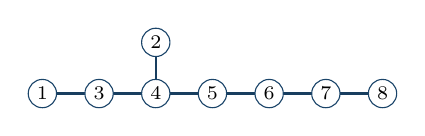
\begin{tikzpicture}[x=.72cm,y=.65cm,baseline=(current bounding box.center)]
 \draw[manifoldblue!68!black,thick]
   (0,0)--(1,0)--(2,0)--(3,0)--(4,0)--(5,0)--(6,0)
   (2,0)--(2,1);
 \foreach \num/\x/\y in {1/0/0,3/1/0,4/2/0,5/3/0,
                            6/4/0,7/5/0,8/6/0,2/2/1}
   \node[circle,draw=manifoldblue!75!black,fill=white,
         inner sep=1.5pt,font=\scriptsize] at (\x,\y) {$\num$};
\end{tikzpicture}
\]
Jej wiodące minory główne wynoszą kolejno
$2,4,6,5,4,3,2,1$. Można to sprawdzić, kolejno
rozwijając wyznacznik po liściu narysowanego
drzewa (Definicja~\ref{def:drzewo-grafowe}):
jeśli usuwamy liść $v$ o jedynym
sąsiedzie $u$, wyznacznik jest
$2\det A_{G-v}-\det A_{G-\{u,v\}}$.
Zatem kryterium Sylvestera daje dodatnią
określoność, a ostatni minor $1$ daje
unimodularność. Dla całkowitego wektora $x$
liczba $x^TE_8x$ jest parzysta, bo składniki
pozadiagonalne występują podwojone. Definiujemy
$\mu(x)=x^TE_8x/2$. Otrzymujemy formę
kwadratową o sygnaturze $8$, a więc
$[E_8]=1\in L_{4j}(\Z)$.
Jest to \emph{przykład algebraiczny}; realizowanie
zadanej formy przez konkretną gładką mapę
normalną wymaga osobnego twierdzenia realizacyjnego.
\end{przyklad}

\subsection*{Wymiary $4j+2$}
Niech $k=2j+1$. Redukcja $P$ modulo $2$
daje przestrzeń symplektyczną
$V=P/2P$ nad $\mathbb F_2$ z formą
$b=\lambda\bmod2$. Funkcja $q=\mu\bmod2$
spełnia
\begin{equation}\label{eq:Arf-q-22}
 q(x+y)=q(x)+q(y)+b(x,y).
\end{equation}
Dla bazy symplektycznej $(e_1,f_1,\dots,e_r,f_r)$
definiujemy
\[
 \operatorname{Arf}(q)
       =\sum_{i=1}^r q(e_i)q(f_i)\pmod2.
\]

\begin{stwierdzenie}[Niezależność od bazy]
\label{prop:Arf-baza-22}
Podany wzór na $\operatorname{Arf}(q)$ nie zależy
od wyboru bazy symplektycznej. Suma ortogonalna
dodaje inwarianty Arfa.
\end{stwierdzenie}
\begin{proof}
Policzmy liczbę niezależną od bazy:
\[
 S(q)=\sum_{x\in V}(-1)^{q(x)}.
\]
Z~\eqref{eq:Arf-q-22} i rozkładu na ortogonalne
płaszczyzny $\langle e_i,f_i\rangle$ wynika,
że $q$ na jednej płaszczyźnie przyjmuje na
$ae_i+bf_i$ wartość
$a q(e_i)+bq(f_i)+ab$, gdzie $a,b\in\mathbb F_2$.
Sumując cztery składniki, dostajemy
\[
 \sum_{a,b\in\mathbb F_2}
  (-1)^{a q(e_i)+bq(f_i)+ab}
     =2(-1)^{q(e_i)q(f_i)}.
\]
Iloczyn tych równości daje
$S(q)=2^r(-1)^{\sum_iq(e_i)q(f_i)}$.
Lewa strona nie używa bazy, więc prawa
wyznacza jednoznacznie Arfa. Dla sumy
ortogonalnej sumy $S$ mnożą się, dlatego
wykładniki znaków, czyli inwarianty Arfa,
dodają się modulo $2$.
\end{proof}

\begin{przyklad}[Dwie formy z tą samą macierzą przecięć]
\label{prz:Arf-dwie-22}
Niech $P=\Z e\oplus\Z f$ i
$\lambda(e,f)=1$, $\lambda(f,e)=-1$,
$\lambda(e,e)=\lambda(f,f)=0$.
Gdy $\mu(e)=\mu(f)=0$, para jest hiperboliczna
i $\operatorname{Arf}(q)=0$. Gdy
$\mu(e)=\mu(f)=1\in\Z/2$, otrzymujemy
$\operatorname{Arf}(q)=1$.
W drugim przypadku wszystkie trzy niezerowe
wektory płaszczyzny nad $\mathbb F_2$ mają
wartość $q=1$, bo
$q(e+f)=1+1+b(e,f)=1$.
Nie ma więc nawet jednowymiarowego
lagranżjanu z $q=0$. Macierz $\lambda$
jest w obu przykładach \emph{identyczna};
o przeszkodzie decyduje dodatkowa informacja
samoprzecięciowa.
\end{przyklad}

W tym wymiarze izomorfizm
$L_{4j+2}(\Z)\cong\Z/2$ przydziela formie
klasę $\operatorname{Arf}(q)$. Dowód, że
\emph{każda} forma z Arfem zerowym jest
stabilnie hiperboliczna, jest algebraiczną
częścią wspomnianego twierdzenia klasyfikacyjnego.

\section{Przykład z jedną nietrywialną pętlą}
\label{sec:L-pi1-Z-22}
\index{rozszczepienie Shanesona}

Pierwszym krokiem poza przypadek $\pi_1=1$
jest grupa nieskończenie cykliczna
$\pi_1=\langle t\rangle\cong\Z$. Jej pierścień
grupowy to pierścień wielomianów Laurenta
$\Z[\Z]=\Z[t,t^{-1}]$. Dla orientowalnej
rozmaitości charakter orientacji ma wartość
$w(t)=1$, a inwolucja używana w formach
przecięcia wysyła $t$ na $t^{-1}$.
Nie można tu zastąpić całego pierścienia
samymi współczynnikami całkowitymi:
wyrazy $t^k$ pamiętają drogi przecięcia
okrążające pętlę $k$ razy, jak w rachunku
$1-t$ w Sekcji~\ref{sec:pi-formy-22}.

\begin{twierdzenie}[Rozszczepienie Shanesona--Ranickiego;
wynik zewnętrzny]
\label{thm:Shaneson-splitting-22}
Niech $G$ będzie grupą z charakterem orientacji
$w:G\to\{\pm1\}$. Przedłużmy go na
$G\times\Z$ tak, aby generator nowego czynnika
zachowywał orientację. Dla $n\geq5$ grupy przeszkód
chirurgicznych spełniają
\begin{equation}\label{eq:Shaneson-splitting-22}
 L_n^s\bigl(\Z[G\times\Z],w\oplus1\bigr)
 \cong L_n^s\bigl(\Z[G],w\bigr)
       \oplus L_{n-1}^h\bigl(\Z[G],w\bigr).
\end{equation}
Drugi składnik ma dekorację $h$; dla dowolnego
$G$ nie należy jej bez dodatkowych hipotez
zamieniać na $s$.
\end{twierdzenie}

Jest to głęboki wynik o rozszczepianiu przeszkody
wzdłuż kierunku okręgu, a nie konsekwencja
formalnego rozpisania macierzy nad
$\Z[t,t^{-1}]$. Wariant geometryczny
\href{https://webhomes.maths.ed.ac.uk/~v1ranick/papers/shan.pdf}
{J.\ L.\ Shanesona, \emph{Wall's Surgery Obstruction
Groups for $G\times\Z$}, twierdzenie 5.1}
zakłada $n\geq7$, $G=\pi_1(K^{n-2})$ dla
zamkniętej gładkiej lub PL rozmaitości $K$
oraz $w=w_1(K)$. Ogólny izomorfizm grup z dekoracjami
$s$ i $h$ podaje
\href{https://webhomes.maths.ed.ac.uk/~v1ranick/papers/splitkl.pdf}
{A.\ Ranicki, \emph{Algebraic and Geometric Splittings
of the K- and L-Groups of Polynomial Extensions}, §6}.
Ranicki rozróżnia też geometryczne i algebraiczne
odwzorowania rozszczepienia; są one zgodne, gdy
$\operatorname{Wh}(G)=0$. Porównaj tabelę w
\href{https://webhomes.maths.ed.ac.uk/~v1ranick/books/scm.pdf}
{C.\ T.\ C.\ Wall, \emph{Surgery on Compact Manifolds},
twierdzenie 13A.8}.

Dla $G=1$ grupa Whiteheada jest zerowa
(Stwierdzenie~\ref{prop:wh-trywialna-20}),
więc dekoracje $s$ i $h$ po prawej stronie
\eqref{eq:Shaneson-splitting-22} się zgadzają.
Zatem z~\eqref{eq:L-Z-22} dostajemy
\begin{equation}\label{eq:L-ZZ-22}
 L_n^s\bigl(\Z[t,t^{-1}],1\bigr)
 \cong L_n(\Z)\oplus L_{n-1}(\Z).
\end{equation}
Rozpisanie dwóch składników, dla $n\geq5$,
daje konkretną tabelę:
\[
\begin{array}{c|cccc}
 n\bmod4&0&1&2&3\\ \hline
 L_n(\Z)&\Z&0&\Z/2&0\\
 L_{n-1}(\Z)&0&\Z&0&\Z/2\\ \hline
 L_n^s(\Z[t,t^{-1}],1)&\Z&\Z&\Z/2&\Z/2.
\end{array}
\]
W nieparzystych wymiarach, w których grupa
jednospójna znika, nowy składnik może więc
pozostać niezerowy. Na przykład dla $n=7$
rachunek daje
$L_7^s(\Z[t,t^{-1}])\cong
L_7(\Z)\oplus L_6(\Z)
=0\oplus\Z/2$;
jest to przesunięty składnik typu Arfa.
Dla $n=9$ otrzymujemy
$0\oplus L_8(\Z)\cong\Z$,
pochodzący z przesuniętego składnika sygnatury.

Nie jest to jeszcze obliczenie przeszkody
konkretnej mapy normalnej. Na przykład
$X=S^1\times S^6$ jest zamkniętą,
orientowalną rozmaitością wymiaru $7$
z $\pi_1(X)=\Z$, lecz jej mapa identycznościowa
z identycznościowymi danymi normalnymi ma
przeszkodę zerową: jest już prostą
równoważnością homotopijną.
Istnienie niezerowego elementu grupy $L_7^s$
nie oznacza, że przeszkoda tej mapy jest niezerowa.
Zbudowanie mapy normalnej o zadanej przeszkodzie
jest osobnym problemem realizacyjnym; w odpowiednim
zakresie wymiarów służą do tego twierdzenia Walla.
Podobnie tabela nie obejmuje generatora
odwracającego orientację, $w(t)=-1$;
algebraiczne grupy można badać także w małych
wymiarach, ale geometryczne kryterium Walla
stosujemy dopiero dla $n\geq5$.

\section{Przeszkoda normalnej mapy i twierdzenie Walla}
\label{sec:tw-Walla-22}

Rozważmy odwzorowanie normalne stopnia jeden
$(f,b):M^n\to X^n$ z
Sekcji~\ref{sec:jadra-chirurgii-21}.
Zakładamy, że $X$ jest zamkniętą gładką
rozmaitością lub skończonym kompleksem
Poincarégo z wybranymi danymi normalnymi.
Po chirurgiach \emph{poniżej} środka można
w dogodnych warunkach doprowadzić $f$ do
wysokiej spójności. W wymiarze parzystym
$n=2k$ pozostałe jądro nad $\Z[\pi]$
z formą $(\lambda_K,\mu_K)$ reprezentuje
\[
 \theta(f,b)=[K,\lambda_K,\mu_K]
       \in L^s_{2k}(\Z[\pi],w).
\]
Bez wcześniejszych chirurgii tę samą klasę
można zdefiniować na całym kompleksie łańcuchów
jako klasę kwadratowego kompleksu Poincarégo.
To ostatnie ujęcie obejmuje też wymiar nieparzysty.
Klasa nie zależy od wybranej kolejności
chirurgii: ślady tych zmian dają kobordyzm
odpowiednich kompleksów kwadratowych.

\begin{twierdzenie}[Twierdzenie Walla o przeszkodzie chirurgicznej]
\label{thm:Wall-L-22}
\index{twierdzenie Walla@Twierdzenie Walla}
Niech $M^n$ i $X^n$ będą spójnymi, zamkniętymi,
gładkimi rozmaitościami, $n\geq5$, i niech
$(f,b):M\to X$ będzie odwzorowaniem normalnym
stopnia jeden z Definicji~\ref{def:normal-map-21},
z danymi normalnymi nad pewną stabilną wiązką
$\xi\to X$ jak w~\eqref{eq:normal-map-21}.
Oznaczmy $\pi=\pi_1(X)$ i przez $w$ charakter
orientacji. Wtedy przeszkoda
$\theta(f,b)\in L^s_n(\Z[\pi],w)$ jest niezmiennikiem
normalnej klasy kobordyzmu.
Równość $\theta(f,b)=0$ zachodzi wtedy i tylko wtedy,
gdy $(f,b)$ jest normalnie kobordantne z prostą
równoważnością homotopijną $f':M'\to X$.
W wersji zwartej z brzegiem zakładamy ponadto,
że odwzorowanie na brzegu jest prostą równoważnością
homotopijną i wykonujemy kobordyzm oraz chirurgie
relatywnie do brzegu.
\end{twierdzenie}

\begin{twierdzenie}[Wersja $h$ i porównanie dekoracji;
 wyniki zewnętrzne]\label{thm:Wall-h-22}
Przy tych samych założeniach o wymiarze $n\geq5$
i danych normalnych, ale z wymaganiem jedynie
\emph{zwykłej} równoważności homotopijnej na brzegu,
istnieje przeszkoda
\[
 \theta^h(f,b)\in L^h_n(\Z[\pi],w).
\]
Zależy ona tylko od normalnej klasy kobordyzmu
relatywnie do brzegu i znika dokładnie wtedy,
gdy tę mapę można przez taki kobordyzm zastąpić
równoważnością homotopijną. Dla pustego brzegu
warunek brzegowy jest oczywiście zbędny.

Jeżeli mapa brzegowa jest prosta, zapomnienie
warunku prostoty daje homomorfizm
$j:L^s_n(\Z[\pi],w)\to L^h_n(\Z[\pi],w)$ oraz
\[
 \theta^h(f,b)=j\bigl(\theta^s(f,b)\bigr).
\]
Jądro i koniec obrazu $j$ opisuje fragment
\emph{ciągu dokładnego Rothenberga}
\begin{equation}\label{eq:Rothenberg-sh-22}
 \cdots\longrightarrow
 \widehat H^{\,n+1}\bigl(\Z/2;\operatorname{Wh}(\pi)\bigr)
 \longrightarrow L^s_n(\Z[\pi],w)
 \xrightarrow{\ j\ } L^h_n(\Z[\pi],w)
 \longrightarrow
 \widehat H^{\,n}\bigl(\Z/2;\operatorname{Wh}(\pi)\bigr)
 \longrightarrow\cdots .
\end{equation}
W grupach Tate'a działa inwolucja dualności
wyznaczona przez $w$ na grupie Whiteheada.
\end{twierdzenie}

Twierdzenie o przeszkodzie w dekoracji $h$
oraz ciąg~\eqref{eq:Rothenberg-sh-22} są tutaj
przyjętymi wynikami zewnętrznymi:
\href{https://www.maths.ed.ac.uk/~v1ranick/surgery/ranicki.pdf}
{Ranicki, \emph{An Introduction to Algebraic Surgery},
 wstęp i przykład 2.16} podaje kryterium
znikania przeszkody oraz warunek brzegowy;
\href{https://www.maths.ed.ac.uk/~v1ranick/books/scm.pdf}
{Wall, \emph{Surgery on Compact Manifolds}, §17D},
odsyła w sprawie ciągu do
\href{https://webhomes.maths.ed.ac.uk/~v1ranick/papers/shan.pdf}
{Shanesona, \emph{Wall's Surgery Obstruction
Groups for $G\times\Z$}, propozycja 4.1}.
Wall sam nazywa swoje porównanie w §17D
zarysem, więc nie używamy go jako pełnego dowodu.
Dokładność~\eqref{eq:Rothenberg-sh-22} pokazuje,
że zniknięcie przeszkody $h$ nie musi usuwać
warunku prostej torsji potrzebnego do wersji $s$.
Gdy $\operatorname{Wh}(\pi)=0$, grupy Tate'a
znikają i $j$ jest izomorfizmem; w szczególności
dotyczy to $\pi=1$.

\begin{przyklad}[Grupy Tate'a dla $C_5$]
\label{prz:Tate-C5-22}
\index{grupa Tate'a!przykład dla $C_5$}
Wróćmy do $R=\Z[C_5]$ i jednostki
$u=1-t-t^{-1}$ z Przykładu~\ref{prz:dekoracje-C5-22}.
\href{https://webhomes.maths.ed.ac.uk/~v1ranick/papers/milnorwh.pdf}
{J.\ Milnor, \emph{Whitehead Torsion}, przykład 6.6}
podaje $\operatorname{Wh}(C_5)\cong\Z$ oraz
generator $[t+t^{-1}-1]=[-u]=[u]$;
ostatnia równość zachodzi, bo $[-1]=0$
w grupie Whiteheada. Ponieważ $\bar u=u$,
inwolucja dualności działa na generatorze
identycznościowo, a więc działa tak na całej
grupie $\operatorname{Wh}(C_5)$.

Oznaczmy tę inwolucję przez $T$. Dla
$A=\operatorname{Wh}(C_5)=\Z\cdot[u]$
mamy $1-T=0$ oraz $1+T=2$. Ze wzorów
definiujących kohomologię Tate'a otrzymujemy
\[
 \widehat H^{2j}(\Z/2;A)
 =\frac{\ker(1-T)}{\operatorname{im}(1+T)}
 =\frac{A}{2A}\cong\Z/2,
 \qquad
 \widehat H^{2j+1}(\Z/2;A)
 =\frac{\ker(1+T)}{\operatorname{im}(1-T)}=0.
\]
Niezerową klasą parzystą jest reszta $[u]$
modulo $2A$. Po podstawieniu do
ciągu~\eqref{eq:Rothenberg-sh-22}, dla
$n\geq6$ parzystego, dostajemy fragment
\[
 0\longrightarrow L^s_n(R,1)
 \xrightarrow{j}L^h_n(R,1)
 \longrightarrow\Z/2\longrightarrow L^s_{n-1}(R,1),
\]
a dla $n\geq5$ nieparzystego
\[
 \Z/2\longrightarrow L^s_n(R,1)
 \xrightarrow{j}L^h_n(R,1)\longrightarrow0.
\]
W parzystym wymiarze $j$ jest zatem injekcją,
a w nieparzystym surjekcją. Dokładność przy
parzystym $n\geq6$ daje ponadto
\[
 0\longrightarrow\operatorname{coker}j_n
 \longrightarrow\Z/2\longrightarrow
 \ker j_{n-1}\longrightarrow0.
\]
Zatem przynajmniej jedna z dwóch sąsiednich map
$j_n,j_{n-1}$ nie jest izomorfizmem, ale rachunek
nie wyznacza, która. Nie rozstrzyga też grup
$L^s_n,L^h_n$ jako grup abstrakcyjnych ani
przeszkody konkretnej mapy normalnej.
\end{przyklad}

\noindent\textbf{Zakres wyprowadzenia.}
Najpierw rozpiszemy argument dostateczności
dla $\pi=1$ i $n=2k\geq6$, a potem
przeprowadzimy wersję nad $\Z[\pi]$.
W wymiarze nieparzystym $n=2k+1\geq5$
zbudujemy przeszkodę z dwóch lagranżjanów
i pokażemy, jak jej zanik prowadzi do chirurgii.
Potrzebne wejścia geometryczne
pochodzą z
\href{https://webhomes.maths.ed.ac.uk/~v1ranick/books/scm.pdf}
{C.~T.~C. Walla, \emph{Surgery on Compact Manifolds},
§§1, 5--6, szczególnie twierdzenia 1.2, 5.2,
5.6, 6.4 oraz lemat 5.7}.
Lemat 5.3 o prostym lagranżjanie dowiedziemy
poniżej; inne użyte wyniki Walla oznaczamy
wprost z ich hipotezami. Wersję z dekoracją
$h$ i zwykłą równoważnością homotopijną
traktujemy oddzielnie jako wynik zewnętrzny;
§17D Walla podaje jedynie szkic porównania
tej dekoracji z wersją $s$.

\noindent\textbf{Cztery kroki dowodu.}
Są to cztery odrębne kroki, a nie samo
wydłużenie rachunku form nad $\Z$:
\begin{enumerate}[label=(\arabic*)]
\item \emph{Chirurgie poniżej środka.}
  Poniżej konstruujemy zgodne obramowanie
  dla pojedynczej klasy w zakresie $2r<n$.
  Skończona indukcja po względnych komórkach
  i kontrola nowych jąder jest treścią
  twierdzenia 1.2 Walla.
\item \emph{Realizacja w środku.}
  W wymiarze parzystym wyliczymy etykiety przecięć i zbudujemy
  bazę hiperboliczną. Zanurzenie sfery w środku
  z warunku $\mu=0$ wymaga obramowanych dysków
  Whitneya; dla wielu sfer trzeba usuwać
  również ich wzajemne przecięcia zgodnie
  z formą $\lambda$ i udoskonaleniem $\mu$;
  używamy tu twierdzenia 5.2 Walla.
\item \emph{Prosta równoważność i niezmienniczość.}
  Zmiana kolejności chirurgii musi dawać
  tę samą klasę przeszkody. Dla ogólnej
  grupy podstawowej wymaga to bazowanych
  kompleksów nad $\Z[\pi]$, kontroli torsji
  Whiteheada i analizy kobordyzmu normalnego.
  Poniżej wyprowadzimy z ciągu dokładnego
  warunek lagranżjanu i rachunek znoszenia
  przecięć na brzegu kobordyzmu. Przygotowanie
  kobordyzmu wymaga twierdzenia 1.4 Walla;
  bazowość, prosta dualność i realizacja
  względnych immersji są osobnymi wejściami
  z jego §§1--2.
\item \emph{Wymiar nieparzysty.}
  Jądra dwóch sąsiednich wymiarów są mierzone
  przecięciem i ilorazem dwóch lagranżjanów
  formacji. Poniżej wyprowadzimy jej ciąg
  dokładny; relacja stabilna i realizacja
  odpowiadających jej ruchów uchwytów
  podamy z jawnym użyciem §6 Walla.
\end{enumerate}
Rachunek poniżej dowodzi kryterium po przyjęciu
wskazanych lematów geometrycznych Walla;
ich własnych dowodów nie przypisujemy temu tekstowi.

\begin{lemat}[Algebraiczny efekt usunięcia jednej pary]
\label{lem:para-Wall-22}
Niech $(K,\lambda,\mu)$ będzie sumą $r$ płaszczyzn
hiperbolicznych nad $\Z$, z bazą
$e_1,f_1,\ldots,e_r,f_r$ taką, że
$\lambda(e_i,f_j)=\delta_{ij}$,
$\lambda(e_i,e_j)=\lambda(f_i,f_j)=0$
oraz $\mu(e_i)=\mu(f_i)=0$.
Wówczas
\[
 e_r^\perp/\Z e_r
 \cong\langle e_1,f_1,\ldots,e_{r-1},f_{r-1}\rangle
\]
jako formy kwadratowe.
\end{lemat}
\begin{proof}
Zapiszmy
$x=\sum_i(a_i e_i+b_i f_i)$.
Z definicji bazy hiperbolicznej
$\lambda(e_r,x)=b_r$. Stąd $x\in e_r^\perp$
dokładnie wtedy, gdy $b_r=0$.
Pozostały współczynnik $a_r$ znika po
przejściu do ilorazu przez $\Z e_r$.
Pary o indeksach $i<r$ są ortogonalne
do $e_r,f_r$, więc ich $\lambda$ i $\mu$
przechodzą do ilorazu bez zmiany.
\end{proof}

\begin{lemat}[Od prostego lagranżjanu do bazy hiperbolicznej]
\label{lem:lagr-hip-Z-22}
Niech $(P,\lambda,\mu)$ będzie nieosobliwą
formą $\epsilon$-kwadratową nad
$\Lambda=\Z[\pi]$, $\epsilon=(-1)^k$.
Załóżmy, że $P$ jest wolny z preferowaną bazą,
a $L\subset P$ jest wolnym lagranżjanem z bazą
$(e_1,\ldots,e_r)$, która przedłuża się do
preferowanej bazy $P$. Niech ponadto
$P/L\to L^*$, $[x]\mapsto\lambda(-,x)|_L$,
będzie prostym izomorfizmem.
Wtedy istnieje preferowana baza
$(e_1,f_1,\ldots,e_r,f_r)$, w której
$\lambda(e_i,f_j)=\delta_{ij}$ oraz
$\lambda(e_i,e_j)=\lambda(f_i,f_j)=0$ i
$\mu(e_i)=\mu(f_i)=0$.
\end{lemat}
\begin{proof}
Wybierzmy podniesienia $f_j^0\in P$ dualnej
bazy $L^*$, zatem
$\lambda(e_i,f_j^0)=\delta_{ij}$.
Jądrem $P\to L^*$ jest $L^\perp=L$,
więc klasy $f_j^0$ są bazą $P/L$.
Założenie o prostocie zapewnia, że
$(e_i,f_j^0)$ reprezentuje preferowaną
klasę baz $P$.

Połóżmy $B_{ij}=\lambda(f_i^0,f_j^0)$
i wybierzmy $m_i\in\Lambda$ reprezentujące
$\mu(f_i^0)$. Zdefiniujmy
\begin{equation}\label{eq:poprawka-lagr-Wall-22}
 f_i=f_i^0-m_i e_i-
       \sum_{j>i}B_{ij}e_j.
\end{equation}
Dodajemy wyłącznie wektory z $L$, toteż
$\lambda(e_i,f_j)=\delta_{ij}$.
Dla $i<j$ składnik $-B_{ij}e_j$ w $f_i$
znosi pierwotne parowanie:
\[
 \lambda(f_i,f_j)=B_{ij}-B_{ij}=0.
\]
Przy $i>j$ używamy hermitowskości.
Ponieważ $\lambda(f_i^0,e_j)=0$ dla $j>i$
i $\lambda(L,L)=0$, równanie
\eqref{eq:quad-add-22} daje
\[
 \mu(f_i)=[m_i]+[\lambda(f_i^0,-m_i e_i)]
   =[m_i-\epsilon\bar m_i]=0.
\]
Równanie~\eqref{eq:quad-diag-22} daje teraz
$\lambda(f_i,f_i)=0$.
Zmiana $f_i^0\mapsto f_i$ jest elementarną
zmianą bazy i nie zmienia jej prostej klasy.
To dowodzi tezy również przy nieprzemiennym
$\Lambda$; dla $\Lambda=\Z$ odzyskujemy
poprzedni rachunek parzystych macierzy
i poprawki Arfa.
\end{proof}

\begin{stwierdzenie}[Przeciwna forma daje odwrotność]
\label{prop:odwrotna-forma-Wall-22}
Jeśli $(P,\lambda,\mu)$ jest prostą
nieosobliwą formą $\epsilon$-kwadratową
na wolnym bazowanym module, to
\[
 (P,\lambda,\mu)\oplus(P,-\lambda,-\mu)
\]
jest formą hiperboliczną. Stąd jej druga
składowa reprezentuje klasę przeciwną
w $L^s_{2k}(\Lambda,w)$.
\end{stwierdzenie}
\begin{proof}
Weźmy diagonalny podmoduł
$\Delta=\{(x,x):x\in P\}\subset P\oplus P$.
Na $\Delta$ obie formy znoszą się:
$\lambda((x,x),(y,y))=0$ oraz
$\mu((x,x))=0$. Jest to bezpośredni
składnik z bazą $(e_i,e_i)$, jeśli
$(e_i)$ jest bazą $P$. Iloraz
$(P\oplus P)/\Delta$ identyfikujemy
z $P$ przez $[(x,y)]\mapsto x-y$.
Parowanie z $\Delta$ jest, z dokładnością
do znaku, izomorfizmem dualności
$P\to P^*$ wyznaczonym przez $\lambda$.
Jest proste z założenia. Lemat
\ref{lem:lagr-hip-Z-22} pokazuje więc,
że $\Delta$ daje bazę hiperboliczną.
\end{proof}

\begin{lemat}[Dlaczego obramowanie istnieje poniżej środka]
\label{lem:ramy-ponizej-srodka-Wall-22}
Niech $(f,b):M^{2k}\to X^{2k}$ będzie
odwzorowaniem normalnym, $k\geq3$, a
$\alpha\in\pi_{r+1}(f)$, gdzie $1\leq r\leq k-1$.
Klasa $\alpha$ ma reprezentanta będącego
zanurzoną $r$-sferą z obramowaniem zgodnym
z danymi normalnymi. Chirurgia na tej sferze
zabija $\alpha$ i nie przywraca jąder
w stopniach mniejszych od $r+1$.
\end{lemat}
\begin{proof}
Reprezentant klasy względnej jest parą
$u:S^r\to M$ i $F:D^{r+1}\to X$ z
$F|_{S^r}=f\circ u$. Ponieważ
$2r<2k$, ogólne położenie pozwala
zastąpić $u$ homotopicznym zanurzeniem:
oczekiwany wymiar jego samoprzecięć
wynosi $2r-2k<0$.

Połóżmy $q=2k-r$. Stabilne dane normalne
$b$ utożsamiają $u^*\nu_M$ z
$(f\circ u)^*\xi$ po stabilizacji.
Ta ostatnia wiązka przedłuża się przez
$F$ nad dyskiem, więc jest stabilnie
trywialna. Ponieważ
$u^*TM\oplus u^*\nu_M$ jest stabilnie
trywialna oraz $TS^r\oplus\R$
jest trywialna, wzór
$u^*TM=TS^r\oplus\nu_u$ pokazuje,
że również $\nu_u$ ma zgodne stabilne
obramowanie. Ponieważ
$q\geq r+2$, można usunąć stabilizację.
Istotnie, $O(q+1)/O(q)\cong S^q$;
długi ciąg homotopii i $(q-1)$-spójność
$S^q$ pokazują, że $O(q)\to O$
jest izomorfizmem na $\pi_j$ dla
$j\leq r$. Dotyczy to zarówno przeszkody
do trywialności $\nu_u$ nad $S^r$,
jak i różnicy dwóch jej obramowań.
Wybieramy rzeczywiste obramowanie.
Jeżeli po zestawieniu go z różniczką
$du:TS^r\to u^*TM$ jego stabilna klasa
różni się od ramy wyznaczonej przez $b$
i $F$ o element $\pi_r(O)$, podnosimy
ten element do $\pi_r(O(q))$ i skręcamy
obramowanie o jego odwrotność.
Otrzymujemy dokładnie zadaną stabilną
klasę ramy, a nie tylko dowolną
trywializację $\nu_u$.

Dysk $F$ i zgodne obramowanie przedłużają
normalne dane przez ślad, zgodnie z
Twierdzeniem~\ref{thm:przedluzenie-mapy-21}.
Ślad ma względem $M$ jeden uchwyt indeksu
$r+1$, który zabija $\alpha$.
Względem nowego brzegu indeks wynosi
$2k-r\geq k+1>r+1$; dlatego ciąg
homotopii pary nie wprowadza nowych
jąder poniżej stopnia $r+1$.
\end{proof}

Przypadek $r=0$ odpowiada dołączeniu uchwytu
indeksu jeden wzdłuż dwóch punktów. Jeżeli
$M$ ma kilka składowych, takimi uchwytami
możemy najpierw je połączyć, przedłużając
mapę wzdłuż wybranych dróg w spójnym $X$.
Ramy obu dysków zaczepienia dobieramy
zgodnie z danymi normalnymi $b$ dokładnie
tak jak w przypadku $h_i=1$ poniżej.

\begin{stwierdzenie}[Skończona redukcja poniżej środka;
 szczególny przypadek twierdzenia 1.2 Walla]
\label{prop:skonczona-redukcja-Wall-22}
Niech $(f,b):M^{2k}\to X^{2k}$ będzie normalnym
odwzorowaniem zwartej rozmaitości gładkiej
bez brzegu,
$k\geq3$, a $X$ niech będzie spójną
przestrzenią o typie skończonego kompleksu
CW z danymi normalnymi wymaganymi dla $(f,b)$.
Istnieje skończony
ciąg chirurgii na sferach wymiarów mniejszych
od $k$, po którym otrzymujemy normalne
odwzorowanie $f':M'\to X$ będące
$k$-spójne. Wszystkie użyte uchwyty mają
indeks co najwyżej $k$.
\end{stwierdzenie}
\begin{proof}
Po ewentualnym połączeniu składowych zakładamy,
że $M$ jest spójna. Z
Twierdzenia~\ref{thm:cw-morse-17} wynika,
że $M$ ma skończony model CW: wybierzmy
równoważność $u:K\to M$ ze skończonym $K$.
Wybieramy również skończony model $L\simeq X$.
Przenosimy $f\circ u$ na mapę $K\to L$,
przybliżamy ją komórkowo i tworzymy
podwójny walec odwzorowań
$M\leftarrow K\to L$. Ma on skończoną
względną strukturę CW nad $M$ i typ
homotopijny zwykłego walca $f$;
oznaczmy ten model przez $C_f$. Wybieramy
jego strukturę komórkową tak, by
$M\hookrightarrow C_f$ było inkluzją,
$C_f\simeq X$, a jego względna struktura
komórkowa nie miała komórek wymiaru zero.
Względne wierzchołki łączymy z $M$
lasem krawędzi, którego każda składowa
spotyka $M$ w jednym wierzchołku,
i zwijamy ten las względem $M$. Wybieramy
równoważność $C_f\to X$, której złożenie
z inkluzją $M$ jest homotopijne z $f$;
dane normalne przenosimy wzdłuż tej homotopii.
Porządkujemy względne komórki wymiarów
co najwyżej $k$ według wymiaru i piszemy
\[
 C_0=M,\qquad C_i=C_{i-1}\cup e^{h_i},
 \qquad 1\leq h_i\leq k.
\]

Indukcyjnie budujemy ślad $W_i$ chirurgii
od $M$ do $M_i$ i równoważność homotopijną
$W_i\simeq C_i$ zgodną z odwzorowaniem do
$C_f$. Dla $i=0$ bierzemy $W_0=M\times I$.
Załóżmy, że zbudowaliśmy $W_{i-1}$.
Komórka $e^{h_i}$ ma odwzorowanie dołączające
$S^{h_i-1}\to C_{i-1}$ i klasę
charakterystyczną w
$\pi_{h_i}(C_i,C_{i-1})$. Dotychczasowe
uchwyty mają indeks co najwyżej $k$.
Po odwróceniu śladu względem $M_{i-1}$
ich indeksy wynoszą co najmniej
\[
 (2k+1)-k=k+1>h_i.
\]
Stąd para $(W_{i-1},M_{i-1})$ jest
$k$-spójna. Po zastąpieniu rozważanych
odwzorowań walcami odwzorowań i użyciu
$W_{i-1}\simeq C_{i-1}$ otrzymujemy,
ponieważ $h_i\leq k$, izomorfizm względnych
klas homotopii
\[
 \pi_{h_i}(C_f,M_{i-1})
 \xrightarrow{\ \cong\ }
 \pi_{h_i}(C_f,C_{i-1}).
\]
Podnosimy nim klasę dysku charakterystycznego
$e^{h_i}$, a nie tylko klasę jego brzegu.
Reprezentant podniesionej klasy składa się
ze sfery $u_i:S^{h_i-1}\to M_{i-1}$
i dysku $D^{h_i}\to C_f$ ją wypełniającego.
Po złożeniu z $C_f\simeq X$ otrzymujemy
klasę względną odwzorowania $f_{i-1}$.
Zgodność podniesienia z klasą
charakterystyczną mówi ponadto, że obraz
$u_i$ w $C_{i-1}$ jest homotopijny
z odwzorowaniem dołączającym komórkę.

Dla $h_i\geq2$
Lemat~\ref{lem:ramy-ponizej-srodka-Wall-22}
realizuje tę klasę przez zanurzoną
obramowaną sferę $S^{h_i-1}$ i chirurgię
z przedłużeniem danych normalnych.
Dla $h_i=1$ sfera $S^0$ składa się
z dwóch punktów, a podniesiony dysk
jest drogą łączącą ich obrazy w $C_f$.
Wiązka normalna nad tą drogą jest
trywialna. Dobieramy małe dyski wokół
obu punktów z ramami zgodnymi ze stabilnymi
danymi $b$; jest to możliwe, bo
$\pi_0 O(2k)\to\pi_0 O$ jest izomorfizmem.
Dołączamy wzdłuż nich uchwyt indeksu jeden
i przedłużamy dane normalne, jak w przypadku
$r=0$ twierdzenia 1.1 Walla.

Nowy ślad powstaje z $W_{i-1}$ przez
dołączenie uchwytu indeksu $h_i$.
Zgodność klasy dołączającej z klasą
komórki i homotopijna niezmienniczość
dołączania komórek dają
$W_i\simeq C_i$ nad $C_f$.

Po ostatniej takiej komórce otrzymujemy
$C_j$. Para $(C_f,C_j)$ nie ma komórek
względnych wymiaru co najwyżej $k$,
więc jest $k$-spójna. Para $(W_j,M_j)$
też jest $k$-spójna, bo wszystkie jej
odwrócone uchwyty mają indeks co najmniej
$k+1$. Zatem złożenie
$M_j\to W_j\simeq C_j\hookrightarrow C_f$
jest $k$-spójne: pierwszy i ostatni człon
mają tę własność przez odpowiednie
ciągi homotopii par, a środkowy jest
równoważnością. Równoważność $C_f\simeq X$
pokazuje, że $f_j:M_j\to X$ jest
$k$-spójne.
Skończoność ciągu wynika ze skończoności
wybranego modelu CW.
\end{proof}

Dowód redukcji używa pojedynczego kroku
geometrycznego z Lematu~\ref{lem:ramy-ponizej-srodka-Wall-22}
i schematu indukcji z
\href{https://webhomes.maths.ed.ac.uk/~v1ranick/books/scm.pdf}
{Walla, §1, twierdzenie 1.2}. Ogólna wersja
obejmuje także inne wymiary i kategorię PL.

\begin{proof}[Rozwinięcie dowodu twierdzenia Walla w przypadku
 $\pi=1$, $n=2k\geq6$]
\textbf{Krok 1: chirurgie poniżej środka.}
Normalne dane $b$ pozwalają przedłużać
odwzorowanie nad śladami chirurgii, jak w
Twierdzeniu~\ref{thm:przedluzenie-mapy-21}.
Lemat~\ref{lem:ramy-ponizej-srodka-Wall-22}
konstruuje zgodne zanurzenie i obramowanie
dla jednej klasy, a
Stwierdzenie~\ref{prop:skonczona-redukcja-Wall-22}
uzasadnia skończone powtarzanie tego kroku.
Po tych operacjach jedynym możliwym
jądrem chirurgii jest środkowe $K_k$.
Identyfikacja $K_k(M)\cong\pi_{k+1}(f)$
i prosta dualność Poincarégo dają
na nim nieosobliwą formę
$(K_k,\lambda,\mu)$ z
Sekcji~\ref{sec:kwadratowa-22}.
Wersja nad $\Lambda$ wymaga dodatkowo
preferowanej stabilnej bazy jądra:
to dokładnie lemat 5.1 Walla.
Podkreślamy, że warunek kwadratowy dotyczy
klas z \emph{normalnym} obramowaniem;
dla dowolnej sfery bez tych danych wzór
na samoprzecięcie ma dodatkowy składnik
Eulera wiązki normalnej (Wall, §5.2).

\textbf{Krok 2: przejście od klasy zerowej do
bazy hiperbolicznej.}
Równość $[K]=0$ w $L_{2k}(\Z)$
oznacza, że dla pewnych $r,s$
forma $K\oplus H_\epsilon^r$ jest
izomorficzna z $H_\epsilon^s$.
Równoważnie, po stabilizacji ma
lagranżjan; przejście od niego do
rzeczywistej bazy z parami $e_i,f_i$
rozpisuje Lemat~\ref{lem:lagr-hip-Z-22}.
Każdą dodawaną
płaszczyznę realizujemy \emph{lokalną}
chirurgią na trywialnej obramowanej
$(k-1)$-sferze: nowa rozmaitość jest
$M\#(S^k\times S^k)$, a dwie sfery
czynnikowe przecinają się raz z
odpowiednim znakiem i mają $\mu=0$.
Ślad dostarcza normalnego kobordyzmu.
To jest lemat 5.5 Walla; wyjaśnia, dlaczego
stabilizacja algebraiczna jest dozwolonym
ruchem geometrycznym. Otrzymujemy bazę
$e_i,f_i$ jak w Lemacie~\ref{lem:para-Wall-22}.

\textbf{Krok 3: jedna rzeczywista chirurgia
w środku.}
Warunek $\mu(e_r)=0$ i
Stwierdzenie~\ref{prop:osadzenie-Wall-52-22},
używające obramowanego triku Whitneya
przy $k\geq3$, dają zanurzoną obramowaną
sferę $S^k\subset M$ reprezentującą $e_r$
oraz dysk w $X$ wypełniający jej obraz.
Wykonujemy chirurgię nad $X$.
Jej ślad $W$ powstaje z $M\times I$
przez dołączenie uchwytu indeksu $k+1$.
Oznaczmy nowy brzeg przez $M'$ i piszmy
$K_i(W)$ dla jądra mapy śladu do $X\times I$.
Oba względne kompleksy uchwytowe mają po
jednym generatorze:
\[
 H_{k+1}(W,M;\Z)\cong\Z,\qquad
 H_k(W,M';\Z)\cong\Z.
\]
W pierwszym ciągu dokładnym mapa brzegu
$\Z\to K_k(M)$ wysyła $1$ na $e_r$.
Jest injektywna, gdyż partner $f_r$ daje
$\lambda(e_r,f_r)=1$, więc $e_r$ jest
prymitywny. Otrzymujemy
\[
 0\longrightarrow\Z e_r\longrightarrow K_k(M)
 \longrightarrow K_k(W)\longrightarrow0.
\]
Od strony $M'$ uchwyt ma indeks $k$.
Złożenie $K_k(M)\to K_k(W)\to
H_k(W,M';\Z)\cong\Z$ mierzy przecięcie
z $e_r$. Dla lewych modułów nad
$\Lambda$ odpowiada mu \emph{liniowy}
homomorfizm
\[
 \ell_{e_r}:K_k(M)\longrightarrow\Lambda,
 \qquad \ell_{e_r}(z)=\epsilon\lambda(z,e_r),
 \quad \epsilon=(-1)^k.
\]
Istotnie, $\ell_{e_r}(az)=a\ell_{e_r}(z)$,
a hermitowskość pokazuje, że jego jądrem
jest $e_r^\perp$. Przy $\Lambda=\Z$ jest to
ten sam wzór co $\lambda(e_r,z)$.
Ponieważ $\lambda(e_r,e_r)=0$, mamy
$\ell_{e_r}(e_r)=0$; mapa przechodzi więc
przez $K_k(W)=K_k(M)/\Z e_r$.
Drugi ciąg dokładny daje
\[
 0\longrightarrow K_k(M')\longrightarrow K_k(W)
 \xrightarrow{\,\ell_{e_r}\,}\Z
 \longrightarrow K_{k-1}(M')\longrightarrow0.
\]
Ponieważ $f_r$ przechodzi na $1$,
$K_{k-1}(M')=0$, a
$K_k(M')\cong e_r^\perp/\Z e_r$.
Forma i udoskonalenie kwadratowe przechodzą
na ten iloraz, gdyż $\mu(e_r)=0$.
W ogólnym przypadku wszystkie wystąpienia
$\Z$ w tych ciągach zastępuje $\Lambda$.
Bez partnera o przecięciu $1$ mógłby
powstać niezerowy $K_{k-1}(M')$.
Lemat~\ref{lem:para-Wall-22} usuwa dokładnie
parę $e_r,f_r$. Powtarzamy ten krok $r$ razy.

\textbf{Krok 4: otrzymanie równoważności.}
Po usunięciu wszystkich par $K_k=0$,
a inne jądra zostały usunięte w Kroku 1
lub znikają przez dualność. Zatem nowa
mapa stopnia jeden jest izomorfizmem
homologii. Ponieważ obie strony są
jednospójne i mają typ kompleksów CW,
twierdzenie Whiteheada
(Twierdzenie~\ref{thm:whitehead})
daje równoważność homotopijną.
Dla $\pi=1$ grupa Whiteheada jest zerowa,
więc jest to równoważność prosta.

\textbf{Konieczność i niezależność wyborów.}
Przeszkoda prostej równoważności wynosi
zero, bo jej kompleks jądra jest ściągalny.
Rozpiszmy rachunek z lematu~5.7 Walla,
który daje niezależność od normalnego
kobordyzmu. Niech ogólniej
$\Phi:(N^{2k+1},M^{2k})\to(Y,X)$ będzie
odwzorowaniem normalnym stopnia jeden
do spójnej prostej pary Poincarégo; wolno
tu dopuścić niespójny brzeg $M$.
W całym rachunku współczynnikiem jest
$\Lambda=\Z[\pi_1(Y)]$, z inwolucją
orientacyjną celu $Y$. Na ewentualnie
niespójnym $M$ formy
$\lambda$ i $\mu$ liczymy na nakryciu
indukowanym z uniwersalnego nakrycia $Y$,
jak w uwadze~5.2.1 Walla. Zakładamy,
że $M\to X$ i $N\to Y$ są $k$-spójne,
$K_k(N,M)=0$, a preferowana stabilna baza
$K_{k+1}(N,M)$ jest reprezentowana przez
rzeczywistą bazę. To dokładne hipotezy
lematu~5.7; samo ich osiągnięcie jest
oddzielnym zadaniem chirurgicznym.

\emph{Krok pierwszy: ciąg i jego bazy.}
Połóżmy
\[
 A=K_{k+1}(N,M),\qquad P=K_k(M),
 \qquad C=K_k(N).
\]
Spójność usuwa niższe jądra, a względna
dualność pozostałe wyższe. Przy
$K_k(N,M)=0$ ciąg długi pary redukuje się do
\begin{equation}\label{eq:wall-57-ciag-22}
 0\longrightarrow A\xrightarrow{\,\partial\,}P
 \xrightarrow{\,i_*\,}C\longrightarrow0.
\end{equation}
Jest to \emph{bazowany} ciąg prostych modułów:
to osobna treść wniosku z lematu~2.4 Walla,
nie własność dowolnego krótkiego ciągu
dokładnego. Wersja dualności Poincarégo
dla kompleksów jądra, lemat~2.6 Walla,
daje prosty izomorfizm $C\cong A^*$.
W lemacie~2.4 bierze się bazowany krótki ciąg
\emph{skończonych kompleksów wolnych} otrzymany
z trzech kompleksów jądra map $M\to X$,
$N\to Y$ i $(N,M)\to(Y,X)$. W naszej sytuacji
wniosek z lematu~2.4 wymaga zaniku
$K_i(N,M)$ poza stopniem $k+1$ i $K_i(N)$
poza stopniem $k$. Ponadto po zmianie
współczynników na dowolny moduł $B$ nad
$\Lambda$ muszą znikać
$K_{k+2}(N,M;B)$ i $K_{k+1}(N;B)$;
oznaczamy tak homologie tych samych
kompleksów jądra ze współczynnikami $B$.
Te hipotezy
zapewniają, że jedyne pozostałe moduły homologii
są stabilnie wolne i mają preferowane klasy baz.
Addytywność torsji dla tego ciągu daje zerową
torsję ciągu~\eqref{eq:wall-57-ciag-22}.
Lemat~2.6 stosuje \emph{prostą} dualność pary
Poincarégo do tych samych kompleksów. Po
redukcji kompleksu jądra $N\to Y$ do jednego
stopnia jego kohomologia to $C^*$; iloczyn
z klasą fundamentalną identyfikuje ją prosto
z $A$. Ponieważ $A$ i $C$ są stabilnie wolne,
dualizacja daje $C\cong A^*$.
Sam
izomorfizm zwykłych grup homologii nie dawałby
ani preferowanych baz, ani prostoty dualności.
Jego wzór w naszej konwencji lewych
modułów rozpoznamy po Kroku 2. Na razie
na całym $P$ określmy
\[
 \widetilde\rho:P\longrightarrow A^*,
 \qquad \widetilde\rho(z)(x)=\lambda(\partial x,z).
\]
Na $A^*=\operatorname{Hom}_\Lambda(A,\Lambda)$
działanie lewe określa
$(a\cdot h)(x)=h(x)\bar a$.
Dlatego $\widetilde\rho(az)=a\cdot
\widetilde\rho(z)$;
strzałka z $\lambda(z,\partial x)$
byłaby przy tej konwencji antyliniowa.

\emph{Krok drugi: znikanie formy.}
Weźmy $x,y\in A$. Obramowane immersje
reprezentujące $\partial x,\partial y$
na $M$ można przedłużyć do obramowanych
immersji $T_x,T_y$ w $N$, których dziedziną
jest suma skończona $(k+1)$-sfer z usuniętymi
dyskami. Zniknięcie klasy brzegowej w $C$
wynika z~\eqref{eq:wall-57-ciag-22};
przejście od tego faktu homologicznego do
takiego \emph{obramowanego} przedłużenia
korzysta ze względnego twierdzenia Hurewicza,
danych normalnych i argumentu z twierdzenia~1.3
Walla. Nie wynika z samego ciągu dokładnego.

Ustawmy $T_x,T_y$ poprzecznie. Ich przecięcie
ma wymiar $(k+1)+(k+1)-(2k+1)=1$,
a więc składa się z okręgów i łuków.
Okręgi nie mają brzegu. Końce łuków
odpowiadają punktom przecięcia
$\partial T_x$ z $\partial T_y$ na $M$.
Po podniesieniu do nakrycia wyznaczonego
przez $\pi_1(Y)$ etykieta $g\in\pi_1(Y)$
jest stała wzdłuż jednego łuku, podczas
gdy orientacja jego dwóch końców daje
przeciwne znaki. Dla każdego $g$ suma
współczynników przy $g$ jest zatem zerem:
\[
 \lambda(\partial x,\partial y)=0.
\]
W szczególności $\widetilde\rho$ znika
na $\partial A$ i przechodzi do
\begin{equation}\label{eq:wall-57-dualnosc-22}
 \rho:C=P/\partial A\longrightarrow A^*,
 \qquad \rho([z])(x)=\lambda(\partial x,z).
\end{equation}
Jest to izomorfizm dualności względnej
z lematu~2.6 Walla, z dokładnością do
stałego znaku wynikającego z konwencji
orientacji. Zgodność dualności względnej,
operatora brzegu i formy przecięcia na $M$
utożsamia ocenę dualną z $\lambda(\partial x,z)$.
Ta zgodność jest osobnym wejściem
geometrycznym z dowodu lematu~5.7 Walla;
sam abstrakcyjny izomorfizm $C\cong A^*$
nie wyznacza wzoru na $\rho$.
Mnożenie przez $-1$ nie zmienia prostej
klasy tego izomorfizmu.

Tak samo ustawmy pojedynczą immersję
$T_x$ w położeniu ogólnym. Jej zbiór
podwójnych punktów ma wymiar jeden;
dla $k\geq2$ można uniknąć punktów
potrójnych przez pozycję ogólną.
Wzdłuż każdego łuku podwójnych punktów
ustalamy kolejność dwóch gałęzi.
Na jego końcach leżą samoprzecięcia
$\partial T_x$ o tej samej etykiecie
$g$ i przeciwnych znakach. Jeśli
zmienimy kolejność gałęzi, oba wkłady
przejdą na równoważne klasy w
$Q_{(-1)^k}(\Lambda)$.
Okręgi znów nie mają końców. Dlatego
\[
 \mu(\partial x)=0.
\]

\emph{Krok trzeci: lagranżjan i klasa $L$.}
Niech $L=\partial A\subset P$.
Z~\eqref{eq:wall-57-ciag-22} mamy $P/L\cong C$,
a~\eqref{eq:wall-57-dualnosc-22} mówi, że
\[
 P/L\xrightarrow{\;[z]\mapsto
           \lambda(-,z)|_L\;}L^*
\]
jest prostym izomorfizmem. Ponieważ
$\lambda|_{L\times L}=0$, jądro mapy
$P\to L^*$ równa się $L$; jest nim
z definicji $L^\perp$. Wraz z
$\mu|_L=0$ daje to lagranżjan kwadratowy.
Preferowana baza $A$ przechodzi na bazę
$L$; prostota dualności daje bazę $C$,
a bazowość~\eqref{eq:wall-57-ciag-22}
pozwala przedłużyć bazę $L$ do
preferowanej bazy $P$.
Lemat~\ref{lem:lagr-hip-Z-22} czyni
$(P,\lambda,\mu)$ formą hiperboliczną.

Teraz stosujemy ten rachunek do
$Y=X\times I$ i $M=\partial N=M_-\sqcup M_+$.
Mapy końców przygotowujemy do
$k$-spójności, mapę $N\to Y$ także,
a odejmowanie uchwytów usuwa
$K_k(N,\partial N)$. Po stabilizacji
preferowana stabilna baza $A$ ma
rzeczywistego reprezentanta.
W nieparzystym wymiarze $2k+1$
twierdzenie~1.4 Walla daje jednocześnie
$k$-spójność map $N\to Y$ i $\partial N\to X$
oraz $(k+1)$-spójność homologiczną mapy par.
W jego dowodzie ostatni warunek uzyskuje się
po zwykłych chirurgiach przez odejmowanie
uchwytów: generatory względnego jądra
przedstawia się obramowanymi dyskami
dochodzącymi do brzegu. Dla nowej mapy
$\Phi_0$ fragment ciągu dokładnego ma postać
\[
 \Lambda^r\longrightarrow H_{k+1}(\Phi)
 \longrightarrow H_{k+1}(\Phi_0)\longrightarrow0.
\]
Pierwsza strzałka jest surjekcją z wyboru
generatorów, więc ostatni moduł znika.
Dodatek do twierdzenia~1.4 pozwala wykonać
te zmiany po stronie $M_+$, zachowując $M_-$;
na brzegu odpowiadają one chirurgiom na
trywialnie obramowanych sferach $S^{k-1}$.
Lemat~5.5 Walla mówi, że każda taka
stabilizacja dodaje do formy $M_+$ standardową
płaszczyznę hiperboliczną. Ten krok zapewnia
też rzeczywiste reprezentanty potrzebnych
stabilnych baz; nie wynika z rachunku
lagranżjanu. Wówczas
\[
 P=K_k(\partial N)
 \cong K_k(M_+)\oplus K_k(M_-)^{-},
\]
gdzie minus oznacza przeciwną formę.
Hiperboliczność $P$ daje
$[K_k(M_+)]=[K_k(M_-)]$.
Tak otrzymujemy niezmienniczość
normalnej klasy kobordyzmu, z jawnym
użyciem twierdzeń~1.3 i~1.4 oraz
lematów~2.4, 2.6 i~5.5 Walla.
\end{proof}

\subsection*{Pełna wersja parzysta nad \texorpdfstring{$\Z[\pi]$}{Z[pi]}}

W tym ustępie $k\geq3$, $n=2k$, $\pi$ jest dowolną grupą,
$w:\pi\to\{\pm1\}$ charakterem orientacji celu, a
$\Lambda=\Z[\pi]$ ma inwolucję
$\overline g=w(g)g^{-1}$. Kładziemy
$\epsilon=(-1)^k$. Moduły są lewe; formę przecięcia
$\lambda:P\times P\to\Lambda$ zapisujemy liniowo w pierwszej
zmiennej, zatem
\[
 \lambda(ax,by)=a\lambda(x,y)\bar b,
 \qquad \lambda(y,x)=\epsilon\overline{\lambda(x,y)}.
\]
Współczynniki $\Lambda$ pochodzą zawsze od grupy podstawowej
\emph{celu}, także wtedy, gdy źródło jest niespójne.

Przez \emph{preferowaną bazę stabilną} modułu jądra rozumiemy
klasę baz uzyskaną z baz komórkowych kompleksu jądra przez
proste redukcje i stabilizacje. Dwie takie bazy mają tę samą
klasę, gdy odpowiednia zmiana bazy ma zerową klasę
w $\operatorname{Wh}(\pi)$. Zwykłe stwierdzenie, że moduł jest
wolny, nie zawiera tej informacji. Po dodaniu dostatecznie wielu
modułów wolnych preferowaną bazę stabilną można reprezentować
rzeczywistą bazą.

\begin{twierdzenie}[Twierdzenie 5.6 Walla w wymiarze parzystym $2k\geq6$]
\label{thm:Wall-parzyste-pelne-22}
Niech $(X,W)$ będzie spójną prostą parą Poincarégo o formalnym
wymiarze $2k\geq6$, $\nu\to X$ wiązką wektorową, a $M^{2k}$
zwartą gładką rozmaitością z brzegiem. Niech
$\phi:(M,\partial M)\to(X,W)$ będzie odwzorowaniem stopnia jeden,
którego ograniczenie $\partial M\to W$ jest prostą równoważnością
homotopijną. Wybierzmy stabilną trywializację
$F:\tau_M\oplus\phi^*\nu\cong M\times\R^N$ dla dostatecznie
dużego $N$.

Po chirurgiach normalnych relatywnie do $\partial M$ można
uczynić $\phi$ $k$-spójnym. Niech $\widetilde X$ będzie
uniwersalnym nakryciem $X$, a $\widetilde M=\phi^*\widetilde X$.
Środkowe jądro
\[
 K_k(M)=\ker\bigl(H_k(\widetilde M;\Z)
                \xrightarrow{\,\phi_*\,}H_k(\widetilde X;\Z)\bigr)
\]
z preferowaną bazą stabilną, formą przecięcia $\lambda$
i udoskonaleniem samoprzecięciowym $\mu$ wyznacza klasę
\[
 \theta(\phi,F)=[K_k(M),\lambda,\mu]
       \in L^s_{2k}(\Lambda,w).
\]
Nie zależy ona od wykonanych chirurgii ani od normalnego
kobordyzmu relatywnie do $\partial M$. Zachodzi
$\theta(\phi,F)=0$ wtedy i tylko wtedy, gdy tę mapę normalną
można przez taki kobordyzm zastąpić mapą, która jest prostą
równoważnością homotopijną. Przeszkoda jest naturalna dla
inkluzji w sensie opisanym na końcu dowodu.
\end{twierdzenie}

Wall definiuje tę klasę już dla $k\geq2$; równoważność
„$\theta=0$ wtedy i tylko wtedy, gdy można ukończyć chirurgię”
wymaga $k\geq3$. Symbol $L_{2k}(\pi)$ w jego §~5 oznacza tutaj
grupę z dekoracją $s$: istotne są proste bazy, prosta dualność
i prosta równoważność końcowa.

\noindent\textbf{Wejścia zewnętrzne.}
Poniższy dowód przyjmuje następujące dokładne wyniki
\href{https://www.maths.ed.ac.uk/~v1ranick/books/scm.pdf}
{Walla, \emph{Surgery on Compact Manifolds}, §§~1--2 i~5}:
twierdzenie~1.2 o chirurgiach poniżej środka relatywnie do
brzegu; twierdzenie~1.4 o przygotowaniu kobordyzmu przez
odejmowanie uchwytów; lematy~2.3, 2.4 i~2.6 o preferowanych
bazach, bazowanych ciągach dokładnych i prostej dualności;
lemat~5.1 o stabilnej bazie i prostej formie środkowego jądra;
twierdzenie~5.2 o przecięciach oraz o zanurzeniu obramowanej
sfery reprezentującej klasę z $\mu=0$ przy $k\geq3$;
twierdzenie~1.1 o klasach regularnej homotopii
obramowanych immersji;
lemat~5.7 o prostym lagranżjanie na brzegu przygotowanego
kobordyzmu. Twierdzenie~1.1 pozwala wykonać chirurgię
na otrzymanej zanurzonej sferze. Są to twierdzenia
geometryczne, a nie wnioski z poniższych dwóch ciągów
dokładnych. W szczególności twierdzenie~5.2 używa
obramowanego triku Whitneya w środku wymiaru.

\begin{lemat}[Sprowadzenie chirurgii na klasie zerowej do dysku]
\label{lem:wall-zero-do-dysku-22}
W hipotezach Twierdzenia~\ref{thm:Wall-parzyste-pelne-22}
niech $k\geq3$, a
$e:S^{k-1}\times D^{k+1}\hookrightarrow\operatorname{int}M$
będzie obramowanym zanurzeniem dopuszczalnym dla
danych normalnych $(\phi,F)$. Jeżeli klasa
wyznaczona przez rdzeń $e$ wraz z wybraną
homotopią zerującą jego obraz w $X$ jest zerem
w $\pi_k(\phi)$, to $e$ można przeprowadzić
izotopią zachowującą obramowanie na model
standardowy w pewnym dysku
$D^{2k}\subset\operatorname{int}M$.
\end{lemat}
\begin{proof}
W dysku wybierzmy standardową sferę
$S^{k-1}=\partial D^k$ z produktowym otoczeniem.
Kontrakcja dysku daje homotopię zerującą
obraz tej sfery w $X$; trywializacja $F$
na dysku wyznacza zgodne obramowanie.
Jest to model klasy zerowej.
Twierdzenie~1.1
\href{https://www.maths.ed.ac.uk/~v1ranick/books/scm.pdf}
{Walla, §1} przypisuje klasie względnej
\emph{jedną klasę regularnej homotopii
obramowanych immersji}. Dlatego $e$ i model
w dysku łączy taka homotopia. Sama zerowość
obrazu sfery w $X$ nie wystarczyłaby do
tego wniosku: potrzebne są wybrana homotopia
zerująca i zgodność ram z danymi normalnymi.

Zastosujmy parametryczne położenie ogólne
do śladu homotopii rdzeni, relatywnie do
jej końców. W rodzinie jednoparametrowej
oczekiwany wymiar zbioru punktów podwójnych
wynosi
\[
 2(k-1)+1-2k=-1.
\]
Możemy więc wybrać ślad bez takich punktów;
każda sfera pośrednia jest zanurzona, a rodzina
rdzeni jest izotopią we wnętrzu $M$.
Rzeczywiste obramowania również dają się
przenieść wzdłuż tej izotopii: ich ranga to
$k+1$, a stabilizacja
$\pi_{k-1}(O(k+1))\to\pi_{k-1}(O)$
jest izomorfizmem, gdyż kolejne ilorazy
$O(q+1)/O(q)$ są sferami $S^q$.
Zgodność stabilnych ram z twierdzenia~1.1
oznacza zatem zgodność ram rzeczywistych.
Zwężamy włókna obu otoczeń rurkowych i
przedłużamy obramowaną izotopię rdzeni
na otoczenia. Jej podparcie omija $\partial M$.
\end{proof}

\begin{lemat}[Co dokładnie dodaje lokalna stabilizacja]
\label{lem:wall-lokalna-stabilizacja-22}
W hipotezach Twierdzenia~\ref{thm:Wall-parzyste-pelne-22}
niech $\phi$ będzie już $k$-spójne. Chirurgia na
dowolnej dopuszczalnej obramowanej $(k-1)$-sferze
reprezentującej zero w $\pi_k(\phi)$ zmienia środkowe
jądro i jego formę według wzoru
\[
 (K_k(M'),\lambda',\mu')
 \cong (K_k(M),\lambda,\mu)
       \perp H_{(-1)^k}(\Lambda),
\]
gdzie nowa płaszczyzna ma preferowaną bazę
$e,f$ z $\lambda(e,f)=1$ i
$\mu(e)=\mu(f)=0$.
\end{lemat}
\begin{proof}
Lemat~\ref{lem:wall-zero-do-dysku-22} sprowadza
tę chirurgię przez obramowaną izotopię do
standardowej chirurgii w dysku.
Lokalny rachunek wykonujemy najpierw w
$S^{2k}=\partial(D^k\times D^{k+1})$.
Jego rozkład brzegowy zawiera
$S^{k-1}\times D^{k+1}$ oraz
$D^k\times S^k$. Zastąpienie pierwszej
części przez drugą w chirurgii daje
dwie kopie $D^k\times S^k$ sklejone po
$S^{k-1}\times S^k$, czyli
$S^k\times S^k$. Dlatego chirurgia w
dysku rozmaitości $M$ daje
$M'\cong M\#(S^k\times S^k)$.
Mapę do $X$ na nowym składniku można
wybrać stałą. W nakryciu indukowanym
z $\widetilde X$ każda kopia tego
składnika dostarcza dwie klasy
$S^k\times\{*\}$ i $\{*\}\times S^k$.
Ich przesunięcia przez elementy $\pi$
tworzą wolny składnik
$\Lambda e\oplus\Lambda f$ w jądrze;
ciąg Mayera--Vietorisa dla sumy
spójnej pokazuje, że nie powstają
relacje ze starym $K_k(M)$.

Obie sfery czynnikowe przecinają się
w jednym punkcie. Ich obramowania pochodzą
z produktowych uchwytów i są zgodne
z danymi normalnymi śladu. Tak obramowane
sfery są zanurzone i nie mają punktów podwójnych.
Twierdzenie~5.2 Walla
o obramowanych immersjach daje zatem
$\lambda(e,f)=1$ oraz $\mu(e)=\mu(f)=0$.
Leżą w dysku
rozłącznym od reprezentantów starego
jądra, więc suma jest ortogonalna.
Nowe generatory pochodzą od
standardowych uchwytów lokalnej
chirurgii; ich macierze przy
kontrakcjach mają jednostki $1$.
Zatem baza $(e,f)$ należy do
preferowanej prostej klasy baz.
\end{proof}

Oba powyższe lematy razem wyprowadzają
lemat~5.5 Walla w używanym tu zakresie,
przy jawnym zastosowaniu jego twierdzenia~1.1.

\begin{proof}[Dowód z wyszczególnieniem wejść Walla]
\textbf{1. Redukcja i właściwy obiekt algebraiczny.}
Twierdzenie~1.2 Walla pozwala przez skończenie wiele
chirurgii relatywnie do brzegu doprowadzić $\phi$ do
$k$-spójności. W tej sytuacji jądra nad $\Lambda$ znikają
poza stopniem $k$. Lemat~5.1 identyfikuje
$K_k(M)$ z odpowiednią względną grupą homotopii i nadaje
mu preferowaną bazę stabilną. Prosta dualność pary
Poincarégo daje prosty izomorfizm $K_k(M)\to K_k(M)^*$.
Nie wynika to z samej $k$-spójności: w zastosowaniu
lematu~2.3(c) Walla potrzebne są również skończoność
kompleksów i zanik pozostałych homologii kompleksu
jądra, a na odpowiednim krańcu zanik z dowolnymi
współczynnikami $\Lambda$-modułowymi. Zapewniają je
prosta dualność Poincarégo, warunek stopnia jeden
i prosta równoważność na brzegu, jak w dowodzie
lematu~5.1 Walla.
Twierdzenie~5.2 konstruuje na tym module formę
$\epsilon$-kwadratową $(\lambda,\mu)$.
To wyjaśnia, dlaczego jej klasę liczymy w $L^s_{2k}$,
a nie wyłącznie w grupie zwykłych form na abstrakcyjnych
modułach.

\textbf{2. Stabilizacja i baza hiperboliczna.}
Jeśli $\theta(\phi,F)=0$, definicja zerowej klasy
w parzystej grupie chirurgicznej mówi, że po dodaniu
pewnej liczby standardowych płaszczyzn hiperbolicznych
otrzymamy prostą formę hiperboliczną. Algebraiczne
przejście od prostego lagranżjanu do preferowanej bazy
hiperbolicznej jest rozpisane w
Lemacie~\ref{lem:lagr-hip-Z-22}; jego hipoteza o prostocie
$P/L\to L^*$ jest potrzebna właśnie dla torsji.

Każdą algebraicznie dodaną płaszczyznę realizuje
chirurgia z
Lematu~\ref{lem:wall-lokalna-stabilizacja-22}.
Możemy więc, po
normalnym kobordyzmie relatywnie do brzegu, założyć
\[
 K_k(M)=\bigoplus_{i=1}^{r}(\Lambda e_i\oplus\Lambda f_i),
 \quad \lambda(e_i,f_j)=\delta_{ij},\quad
 \lambda(e_i,e_j)=\lambda(f_i,f_j)=0,
 \quad \mu(e_i)=\mu(f_i)=0.
\tag{H}
\]
Baza $(e_1,f_1,\ldots,e_r,f_r)$ jest preferowana,
nie tylko dowolna.

\textbf{3. Jedna chirurgia środkowa i jej dwa ciągi.}
Lemat~5.1 i twierdzenie~5.2 przedstawiają $e_r$
przez obramowaną immersję $S^k\looparrowright M$.
Równość $\mu(e_r)=0$ pozwala, gdy $k\geq3$,
zastąpić ją obramowanym zanurzeniem
$S^k\hookrightarrow M$ reprezentującym tę samą klasę
jądra. Chirurgia nad $X$ według twierdzenia~1.1
ma ślad $T$ i nowy brzeg $M'$. Kompleks pary
$(T,M)$ ma jeden generator w stopniu $k+1$,
a kompleks pary $(T,M')$ jeden generator w stopniu $k$;
w obu przypadkach współczynnikiem jest $\Lambda$.

Pierwszy ciąg pary, z uwzględnieniem jądra mapy
do celu, zawiera strzałkę $\Lambda\to K_k(M)$,
która wysyła $1$ na $e_r$. Jest injektywna,
ponieważ $e_r$ należy do bazy (H). Otrzymujemy
\begin{equation}\label{eq:Wall-parz-pierwszy-22}
 0\longrightarrow\Lambda e_r\longrightarrow K_k(M)
  \longrightarrow K_k(T)\longrightarrow0.
\end{equation}
Od drugiego końca uchwytu dostajemy
\begin{equation}\label{eq:Wall-parz-drugi-22}
 0\longrightarrow K_k(M')\longrightarrow K_k(T)
  \xrightarrow{\,\ell_{e_r}\,}\Lambda
  \longrightarrow K_{k-1}(M')\longrightarrow0.
\end{equation}
Strzałka $\ell_{e_r}$ mierzy przecięcie z osią
dołączonego uchwytu. Przy naszej konwencji lewych
modułów jest indukowana przez
\[
 \ell_{e_r}(z)=\epsilon\lambda(z,e_r)
 \qquad(z\in K_k(M)).
\]
Jest liniowa w $z$, znika na $e_r$ i
$\ell_{e_r}(f_r)=
\epsilon\lambda(f_r,e_r)=\epsilon^2=1$.
Ta ostatnia równość daje rozszczepienie strzałki
w~\eqref{eq:Wall-parz-drugi-22}, a więc
$K_{k-1}(M')=0$. Jej jądro w~$K_k(M)$ to
$e_r^\perp=\{z:\lambda(z,e_r)=0\}$, skąd
\begin{equation}\label{eq:Wall-parz-iloraz-22}
 K_k(M')\cong e_r^\perp/\Lambda e_r
   \cong\bigoplus_{i<r}(\Lambda e_i\oplus\Lambda f_i).
\end{equation}
Ponieważ $\mu(e_r)=0$ i forma znika między
$e_r$ a $e_r^\perp$, udoskonalenie $\mu$
przechodzi na ten iloraz. Jest to dokładnie forma
hiperboliczna na pozostałych parach, z ich
preferowaną bazą.

Ostatnie zdanie wymaga kontroli \emph{prostej}
klasy bazy. Na płaszczyźnie $e_r,f_r$ obie
strzałki tworzą bazowany kompleks
\[
 0\longrightarrow\Lambda e_r
 \xrightarrow{\,e_r\mapsto e_r\,}
 \Lambda e_r\oplus\Lambda f_r
 \xrightarrow{\,e_r\mapsto0,\;f_r\mapsto1\,}
 \Lambda\longrightarrow0.
\]
Jego macierze zawierają jednostkę $1$, więc
elementarna kontrakcja ma zerową torsję
Whiteheada. Geometryczne bazy komórek uchwytowych
i bazowany wniosek z lematu~2.4 Walla pozwalają
przenieść ten rachunek na preferowane stabilne
bazy kompleksów jądra.
Dlatego izomorfizm~\eqref{eq:Wall-parz-iloraz-22}
zachowuje preferowaną klasę bazy; zwykły
izomorfizm modułów nie wystarczałby do tego wniosku.

Powtarzając krok dla $e_{r-1},\ldots,e_1$,
usuwamy całe $K_k$ i nie tworzymy niższego jądra.
Końcowa mapa jest $k$-spójna i ma zerowe homologie
kompleksu jądra nad $\Lambda$, zatem jest
równoważnością homotopijną przez twierdzenie
Whiteheada z lokalnymi współczynnikami.
Preferowane bazy i powyższe elementarne kontrakcje
dają zerową torsję jej stożka, czyli równoważność
jest \emph{prosta}. To kończy dostateczność.

\textbf{4. Konieczność i niezależność od wyborów.}
Jeśli końcowa mapa jest prostą równoważnością
homotopijną, jej bazowany kompleks jądra jest
prosto ściągalny. Jego klasa w $L^s_{2k}$ wynosi zero.

Dla niezmienniczości porównajmy dwie przygotowane
$k$-spójne mapy normalne $M_-\to X$ i $M_+\to X$
połączone normalnym kobordyzmem relatywnie do brzegu.
Jego celem jest para $(Y,X_0)$, gdzie
$Y=X\times I$ oraz
$X_0=X\times\{0,1\}\cup W\times I$.
Walla twierdzenia~1.2 i~1.4 pozwalają tak przygotować
mapę śladu $N^{2k+1}\to Y$, aby zarówno ona,
jak i mapa całego brzegu $\partial N\to X_0$
były $k$-spójne oraz aby $K_k(N,\partial N)=0$;
konieczne
zmiany na końcach dodają tylko płaszczyzny
hiperboliczne z lematu~5.5. Można następnie
stabilizować tak, by preferowana stabilna baza
$A=K_{k+1}(N,\partial N)$ była reprezentowana
przez rzeczywistą bazę. Wszystkie te operacje
są geometryczną treścią wymienionych twierdzeń,
nie konsekwencją samej algebraicznej klasy $\theta$.

Zapiszmy $P=K_k(\partial N)$ i $C=K_k(N)$;
wszystkie grupy liczymy nad
$\Z[\pi_1(X\times I)]=\Lambda$. Ponieważ
mapa na bocznym brzegu jest prostą równoważnością,
\[
 (P,\lambda,\mu)
  \cong (K_k(M_+),\lambda_+,\mu_+)
       \oplus(K_k(M_-),-\lambda_-,-\mu_-).
\]
W tej sytuacji bazowany ciąg dokładny ma postać
\begin{equation}\label{eq:Wall-parz-lagr-ciag-22}
 0\longrightarrow A\xrightarrow{\,\partial\,}P
   \longrightarrow C\longrightarrow0.
\end{equation}
\emph{Bazowanie} tego ciągu jest wnioskiem z~2.4
Walla, a prosta dualność $C\cong A^*$ z~2.6.
Diagram dualności Poincarégo utożsamia powstałe
$P/\partial A\cong C\cong A^*$ z odwzorowaniem
$[p]\mapsto(a\mapsto\lambda(\partial a,p))$;
stąd jego prostota jest właśnie prostotą
dualności formy na ilorazie.
Lemat~5.7 Walla mówi więcej: $\partial A$ jest
\emph{prostym lagranżjanem} formy na~$P$,
czyli $\lambda|_{\partial A}=0$,
$\mu|_{\partial A}=0$, jego preferowana baza
przedłuża się do preferowanej bazy $P$,
a indukowana dualność $P/\partial A\to A^*$
jest prosta. Jego dokładne hipotezy to: mapa normalna
stopnia jeden $(N,\partial N)\to(Y,X_0)$ ze zwartej
rozmaitości $N$ do prostej pary Poincarégo ze
spójnym $Y$, z danymi $\nu,F$ jak wyżej,
$\dim N=2k+1\geq5$, $k$-spójność map
$N\to Y$ i $\partial N\to X_0$,
$K_k(N,\partial N)=0$ oraz rzeczywista baza
reprezentująca preferowaną bazę stabilną
$K_{k+1}(N,\partial N)$. W zastosowaniu
$Y=X\times I$; przy ogólnej parze $(Y,X_0)$
trzeba używać $\Z[\pi_1(Y)]$, nie
$\Z[\pi_1(X_0)]$.

Lemat~5.3 Walla, czyli algebraiczny
Lemat~\ref{lem:lagr-hip-Z-22}, czyni formę
na~$P$ hiperboliczną. Z~\eqref{eq:Wall-parz-lagr-ciag-22}
i znaku orientacji obu końców wynika zatem
$[K_k(M_+)]=[K_k(M_-)]$ w $L^s_{2k}(\Lambda,w)$.
To dowodzi niezależności od kobordyzmu oraz,
biorąc kobordyzmy realizujące różne przygotowania,
od wyboru chirurgii poniżej środka.

\textbf{5. Naturalność dla inkluzji.}
Niech przy $W\subset X$ do pary $(X,W)$ będzie
doklejona triada przez prostą równoważność
homotopijną triad, jak w ostatnim akapicie dowodu
twierdzenia~5.6 Walla. Dla $X\hookrightarrow X'$
otrzymujemy homomorfizm grup i pierścieni
$\rho:\Z[\pi_1X]\to\Z[\pi_1X']$ zgodny
z charakterami orientacji. Nowa część triady
ma prosto ściągalny kompleks jądra, więc po
zmianie współczynników jądro starej części,
jego preferowana baza oraz liczby przecięć
i samoprzecięć przechodzą odpowiednio na
$\Z[\pi_1X']\otimes_{\Lambda}K_k(M)$,
$\rho(\lambda)$ i $\rho(\mu)$. Stąd
\[
 \theta(\phi\cup\phi',F\cup F')
       =\rho_*\theta(\phi,F)
       \quad\text{w }L^s_{2k}(\Z[\pi_1X'],w').
\]
Nie jest to stwierdzenie o dowolnym odwzorowaniu
celów: chodzi o tę konkretną inkluzję z dołączoną
prostą równoważnością triad.
\end{proof}

\noindent\textbf{Zakres dowodu.}
Rachunek~\eqref{eq:Wall-parz-pierwszy-22}--
\eqref{eq:Wall-parz-iloraz-22}, usunięcie pary
hiperbolicznej oraz jej elementarna torsja są
wyprowadzone powyżej. Istnienie wymaganych
obramowanych zanurzeń, przygotowanie kobordyzmu,
preferowane bazy i prosta dualność są użytymi
z dokładnymi hipotezami wynikami Walla.
Fragment zamyka \emph{parzysty} przypadek $n\geq6$;
przypadek nieparzysty używa formacji i odrębnych
twierdzeń jego §~6.

\begin{figure}[htbp]
\centering
\begin{tikzpicture}[>=Latex,font=\small,
 box/.style={draw=manifoldblue!75!black,rounded corners=3pt,
 fill=manifoldblue!9,align=center,minimum height=1.05cm,
 text width=2.4cm}]
 \node[box] (a) at (0,0) {normalna mapa\\$M\to X$};
 \node[box] (b) at (3.25,0)
   {chirurgie poniżej\\środka};
 \node[box] (c) at (6.50,0)
   {forma jądra\\$(K,\lambda,\mu)$};
 \node[box] (d) at (9.75,0)
   {lagranżjan i\\chirurgie środkowe};
 \draw[->,thick,manifoldblue!75!black]
   (a)--(b);
 \draw[->,thick,manifoldblue!75!black]
   (b)--(c);
 \draw[->,thick,manifoldblue!75!black]
   (c)--(d);
 \draw[->,thick,manifoldgold!85!black]
   (d.south) -- ++(0,-1.30) -| (a.south);
 \node[fill=white,font=\scriptsize,align=center]
   at (4.85,-1.30) {zanik jądra daje równoważność};
\end{tikzpicture}
\caption{Kolejne etapy twierdzenia Walla w parzystym wymiarze.
Przejście od algebraicznego lagranżjanu do zanurzonych
sfer wymaga lematów geometrycznych Walla.}
\label{fig:mechanizm-Wall-22}
\end{figure}

\subsection*{Dlaczego wymiar nieparzysty wymaga formacji}
Niech $n=2k+1\geq5$ i niech mapa normalna
została przygotowana chirurgiami poniżej
środka. Po stabilizacji wybieramy rozłączne
obramowane reprezentanty generatorów
$K_k(M)$, z otoczeniem
$U=\coprod(S^k\times D^{k+1})$.
To wybranie, wraz z kontrolą prostych baz,
jest geometrycznym krokiem z §6 Walla.
Połóżmy $C=\overline{M\setminus\operatorname{int}U}$.
Moduł $H=K_k(\partial U)$ ma formę
hiperboliczną: na każdej składowej brzegu
$S^k\times S^k$ dwie sfery czynnikowe
przecinają się raz. Po wyborze dróg bazowych
dają bazę $e_1,f_1,\ldots,e_r,f_r$ z
$\lambda(e_i,f_j)=\delta_{ij}$ oraz
$\mu(e_i)=\mu(f_i)=0$.
W obrazie odwzorowań brzegu dostajemy
dwa lagranżjany
\[
 L_0=\operatorname{im}\bigl(K_{k+1}(U,\partial U)
                  \to H\bigr),\qquad
 L_1=\operatorname{im}\bigl(K_{k+1}(C,\partial U)
                  \to H\bigr).
\]
Formacja jest trójką $(H;L_0,L_1)$.
Pierwszy lagranżjan jest jawnie rozpięty przez
jedną rodzinę sfer czynnikowych. Dla drugiego
samo zapisanie go jako obrazu strzałki
\emph{nie} dowodzi warunku $L_1=L_1^\perp$.
Wall najpierw przesuwa obraz $U$ do dysku w~$X$,
przygotowuje parę $(C,\partial U)$ oraz jej
bazy, a następnie stosuje lemat~5.7 do tej pary.
Prostota bazy $L_1$ korzysta tu z lematów~2.4
i~2.6 oraz ze stabilizacji przez dołożenie
reprezentantów generatorów. Ta część konstrukcji
pozostaje wejściem geometrycznym z~§6 Walla.
Jej użycie nie oznacza, że dwa sąsiednie
jądra \emph{są} lagranżjanami; powstają
z ich wzajemnego położenia.

Algebraiczny ciąg
\begin{equation}\label{eq:formacja-ciag-Wall-22}
 0\longrightarrow L_0\cap L_1
 \longrightarrow L_1
 \longrightarrow H/L_0
 \longrightarrow H/(L_0+L_1)
 \longrightarrow0
\end{equation}
jest dokładny: środkowa strzałka wysyła
$z$ na $[z]$, więc jej jądrem jest
$L_0\cap L_1$, a jej obrazem
$(L_0+L_1)/L_0$.
Diagram Mayera--Vietorisa dla $M=U\cup C$
identyfikuje skrajne człony z
$K_{k+1}(M)$ i $K_k(M)$, odpowiednio.
Jeśli $L_0\oplus L_1=H$, oba te jądra
znikają; po zaniku niższych jąder i
przy $\pi_1=1$ twierdzenie Whiteheada
daje równoważność prostą.

Można obliczać oba skrajne człony jedną
macierzą. Po wyborze baz $H=E\oplus E^*$,
$L_0=E$, a prosta izometria $\alpha:H\to H$
przenosi $E$ na $L_1$; jej istnienie dla
prostych lagranżjanów to wniosek~5.3.1 Walla.
Zdefiniujmy
\[
 T=\operatorname{pr}_{E^*}\circ\alpha|_E:
 E\longrightarrow E^*.
\]
Ponieważ iloraz $H/L_0$ jest kanonicznie
$E^*$, środkowa strzałka
\eqref{eq:formacja-ciag-Wall-22}, po
utożsamieniu $L_1$ z $E$ przez $\alpha$,
jest dokładnie $T$. Zatem
\[
 K_{k+1}(M)\cong\ker T,\qquad
 K_k(M)\cong\operatorname{coker}T.
\]
To jest rachunek jąder dla \emph{wybranej}
formacji. Niezależność jej stabilnej klasy
od $U$ oraz wpływ chirurgii na $\alpha$
wymagają osobnych ruchów z~§6 Walla.

Na przykład dla $\epsilon=-1$ weźmy
$H=\Z e\oplus\Z f$ z
$\lambda(e,f)=1$ oraz
$\mu(ae+bf)=ab\pmod2$.
Podmoduły $L_0=\Z e$ i
$L_1=\Z(e+2f)$ są lagranżjanami:
$\mu(e+2f)=0$, a wektor $e+2f$
jest prymitywny. Tutaj $T$ jest
mnożeniem przez $2$: strzałka
$L_1\to H/L_0\cong\Z f$ z
\eqref{eq:formacja-ciag-Wall-22} jest
mnożeniem przez $2$. Jej cokernel to
$\Z/2$, zatem sam fakt istnienia dwóch
lagranżjanów nie oznacza, że obecne
jądro już znikło. Mimo to \emph{klasa tej
formacji jest zerowa}: weźmy jednoelementowy
moduł $K=\Z e$ z parzystą formą
$\gamma(e,e)=2$ i jej udoskonaleniem
kwadratowym $\mu_\gamma(e)=1$.
W hiperbolicznym $K\oplus K^*$ wykres
odwzorowania $\gamma:K\to K^*$ jest
$\Z(e+2f)$. Nasza para $(L_0,L_1)$ jest więc
\emph{formacją brzegową} $\partial\gamma$,
która z definicji reprezentuje zero w grupie
$L^s_{2k+1}(\Z)$. Ten rachunek pokazuje
konkretnie różnicę między zerem przeszkody
a zanikiem jąder przed wykonaniem dalszych
chirurgii.

Przesunięcie uchwytu ma czytelny rachunek
w $H_\epsilon\oplus H_\epsilon$:
$e_1\mapsto e_1+e_2$ oraz
$f_2\mapsto f_2-f_1$, przy pozostałych
wektorach stałych, zachowuje wszystkie
parowania i $\mu$. Pełna relacja formacji
obejmuje ponadto stabilizację i formacje
brzegowe. Dlatego zerowa \emph{klasa} w
$L^s_{2k+1}(\Lambda,w)$ nie wymaga, aby
wybrane już teraz $L_0$ i $L_1$ były
dopełniające. Realizacja dozwolonych
ruchów przez chirurgie oraz niezależność
wyboru $U$ to treść
\href{https://webhomes.maths.ed.ac.uk/~v1ranick/books/scm.pdf}
{Walla, §6, twierdzenia 6.4 i 6.6};
algebraiczną relację formacji wyjaśnia
\href{https://www.maths.ed.ac.uk/~v1ranick/papers/ranicki.pdf}
{A.\ Ranicki, \emph{An Introduction to Algebraic Surgery}, §9}.

\subsection*{Pełne kryterium chirurgiczne w wymiarze nieparzystym}

Niech $m=2k+1\geq5$, niech
$\pi=\pi_1(X)$ i niech $w:\pi\to\{\pm1\}$ będzie
homomorfizmem orientacji. Na pierścieniu
$\Lambda=\Z[\pi]$ stosujemy antyinwolucję
\[
 \overline{\sum_g n_g g}=\sum_g n_g w(g)g^{-1},
 \qquad \epsilon=(-1)^k.
\]
W tym podrozdziale wszystkie moduły są lewymi
$\Lambda$-modułami. Oznaczenia formy
$\epsilon$-kwadratowej i lagranżjanu są takie jak
w~Definicji~\ref{def:forma-kwadratowa-22} i
Definicji~\ref{def:hiperboliczna-22}. Dla czytelnika
kluczowa różnica względem wymiaru parzystego jest
następująca: dwa środkowe jądra jednej mapy
powstają z \emph{wzajemnego położenia dwóch
lagranżjanów} w jednym module hiperbolicznym.

\paragraph{Grupa algebraiczna.}
Niech $E=\Lambda^r$ z ustaloną bazą i niech
$E^*=\operatorname{Hom}_\Lambda(E,\Lambda)$, z
lewym działaniem $(a\varphi)(x)=\varphi(x)\bar a$.
Na $H_\epsilon(E)=E\oplus E^*$ połóżmy
\[
 \lambda\bigl((x,\varphi),(y,\psi)\bigr)
   =\psi(x)+\epsilon\overline{\varphi(y)},
 \qquad
 \mu(x,\varphi)=[\varphi(x)]\in
 Q_\epsilon(\Lambda)
 =\Lambda/\{a-\epsilon\bar a:a\in\Lambda\}.
\]
Iloraz w ostatnim wzorze jest ilorazem grup
addytywnych. Dla bazy $e_i$ modułu $E$ i jej
bazy dualnej $f_i$ mamy
$\lambda(e_i,f_j)=\delta_{ij}$ oraz
$\mu(e_i)=\mu(f_i)=0$.

Piszemy $SU_r(\Lambda)$ na grupę automorfizmów
$(H_\epsilon(E),\lambda,\mu)$ zachowujących
wyróżnioną prostą klasę baz. Słowo „prosty”
oznacza tutaj zerową torsję Whiteheada
automorfizmu modułu; skrót $SU$ nie określa
wyznacznika. Wyróżniamy podgrupy
\[
 TU_r(\Lambda)=\{A\in SU_r(\Lambda):
             A(E)=E,\ A|_E\text{ jest prosty}\},
 \qquad
 UU_r(\Lambda)=\{A\in TU_r(\Lambda):A|_E=1\}.
\]
Ograniczenie do $E$ daje rozszczepiony ciąg
\[
 1\longrightarrow UU_r(\Lambda)
 \longrightarrow TU_r(\Lambda)
 \longrightarrow\operatorname{Aut}^{s}_\Lambda(E)
 \longrightarrow1.
\]
Rozszczepienie wysyła $B$ na automorfizm
hiperboliczny
$H(B)(x,\varphi)=(Bx,\varphi\circ B^{-1})$.
W bazie $e_i,f_i$ element $UU_r$ ma postać
\[
 u_C(x,\varphi)=(x+C\varphi,\varphi),
 \qquad C=D-\epsilon D^*,
\]
gdzie $D^*$ jest macierzą sprzężoną i
transponowaną. Sam warunek zachowania
$\lambda$ daje tylko $C+\epsilon C^*=0$;
postać $D-\epsilon D^*$ uwzględnia dodatkowo
zachowanie $\mu$ na przekątnej.

Niech $\sigma\in SU_1(\Lambda)$ zamienia dwa
standardowe lagranżjany według wzorów
$\sigma(e)=f$ i $\sigma(f)=\epsilon e$; zatem
$\sigma^2=\epsilon\,1$. Grupy $SU(\Lambda)$,
$TU(\Lambda)$ otrzymujemy przez stabilizację
sumą ortogonalną z identycznością na jednej
płaszczyźnie hiperbolicznej. Niech
\[
 RU(\Lambda)=\langle TU(\Lambda),\sigma\rangle
       \subset SU(\Lambda).
\]
Nie zakładamy tu z góry normalności $RU$.
\href{https://www.maths.ed.ac.uk/~v1ranick/books/scm.pdf}
{Lemat 6.2 i twierdzenie 6.3 Walla, §6}
dają kolejno, po stabilizacji,
$A\oplus A^{-1}\in RU(\Lambda)$ dla każdego
$A\in SU(\Lambda)$ oraz
$[SU(\Lambda),SU(\Lambda)]\subset RU(\Lambda)$.
Stąd $RU$ jest normalna, a
\[
 L^s_{2k+1}(\Lambda,w)
       :=SU(\Lambda)/RU(\Lambda)
\]
jest grupą abelową. W dowodzie Walla lemat~6.2
jest jawną tożsamością blokowych macierzy
hiperbolicznych; twierdzenie~6.3 używa jej do
wykazania normalności. Te dwa wyniki algebraiczne
są tutaj cytowanymi lematami zewnętrznymi.
W poniższym zapisie automorfizmy składamy jak
odwzorowania: $(AB)(x)=A(Bx)$. Wall zapisuje
działanie macierzy na bazach z prawej, dlatego
kolejność czynników w jego wzorach dla kosetów
jest odwrotna.

\begin{twierdzenie}[Wall, twierdzenie 6.4:
                    przypadek nieparzysty]
\label{thm:wall-odd-22}
Niech $(X,W)$ będzie spójną prostą parą Poincarégo
w formalnym wymiarze $m=2k+1\geq5$, a $\nu$ wiązką
stabilną nad $X$. Niech $M^m$ będzie zwartą gładką
rozmaitością z brzegiem, zaś
$f:(M,\partial M)\to(X,W)$ odwzorowaniem stopnia
jeden, którego ograniczenie
$\partial M\to W$ jest prostą równoważnością
homotopijną. Niech $F$ będzie stabilną
trywializacją $TM\oplus f^*\nu$.
Istnieje klasa
\[
 \theta(f,F)\in L^s_m(\Z[\pi_1(X)],w),
\]
która zależy tylko od klasy kobordyzmu normalnego
$(f,F)$ relatywnie do brzegu. Klasa ta jest zerowa
wtedy i tylko wtedy, gdy $(f,F)$ jest normalnie
kobordantne relatywnie do brzegu z prostą
równoważnością homotopijną. Przeszkoda jest
naturalna przy inkluzji par Poincarégo, dla której
dane brzegowe przedłużają się przez prostą
równoważność homotopijną.
\end{twierdzenie}

\begin{lemat}[Rozłączne sfery w nieparzystym wymiarze]
\label{lem:wall-odd-rozlaczne-sfery-22}
W hipotezach Twierdzenia~\ref{thm:wall-odd-22}
załóżmy, że $f$ jest już $k$-spójne.
Każda skończona rodzina klas
$x_1,\ldots,x_r\in\pi_{k+1}(f)$, wraz
z drogami bazowymi i homotopiami zerującymi
ich obrazy w $X$, ma reprezentantów w postaci
parami rozłącznych obramowanych zanurzeń
\[
 e_i:S^k\times D^{k+1}\hookrightarrow
       \operatorname{int}M.
\]
Dla $U=\bigcup_i e_i(S^k\times D^{k+1})$
można po homotopii $f$ relatywnie do $\partial M$
przyjąć $f(U)=*$, zachowując dane normalne.
\end{lemat}
\begin{proof}
Klasę $x_i$ przedstawiamy parą
$u_i:S^k\to M$ i $H_i:D^{k+1}\to X$,
gdzie $H_i|_{S^k}=f\circ u_i$.
Przez kołnierz brzegu przesuwamy obrazy
$u_i$ do wnętrza $M$.
\href{https://www.maths.ed.ac.uk/~v1ranick/books/scm.pdf}
{Twierdzenie 1.1 Walla} wyznacza z $H_i$
i stabilnych danych $F$ klasę regularnej
homotopii obramowanych immersji pogrubień
$S^k\times D^{k+1}\looparrowright M$.
Wybieramy takie immersje i nadal oznaczamy
ich rdzenie przez $u_i$.
Homotopie $H_i$ przenosimy wzdłuż homotopii
rdzeni, tak by nadal zachodziło
$H_i|_{S^k}=f\circ u_i$ i klasy $x_i$
pozostały te same.
W szczególności obramowanie ma być zgodne
z \emph{wybraną} homotopią zerującą, a nie
tylko z klasą samego odwzorowania $u_i$.

Możliwość wyboru rzeczywistych ram widać
również bezpośrednio. Wiązka $H_i^*\nu$
nad dyskiem jest trywialna, zatem $F$
i $TS^k\oplus\R\cong\R^{k+1}$ dają
stabilne obramowanie wiązki normalnej
rdzenia $u_i$, rangi $k+1$.
Inkluzja $O(k+1)\to O$ indukuje izomorfizm
na $\pi_{k-1}$, więc stabilnie trywialna
wiązka nad $S^k$ jest rzeczywiście trywialna.
Na $\pi_k$ ta inkluzja jest surjekcją;
skręcając rzeczywiste obramowanie, można
więc dopasować jego klasę stabilną do $F$
i $H_i$. Oba stwierdzenia wynikają z ciągów
homotopii dla $O(q)\to O(q+1)\to S^q$.

Ustawiamy jednocześnie wszystkie rdzenie
w położeniu ogólnym, nie zmieniając ich klas.
Wymiar oczekiwanych przecięć własnych
i wzajemnych jest
$2k-(2k+1)=-1$; rdzenie są więc zanurzone
i parami rozłączne. Skończoność rodziny
pozwala zwęzić włókna $D^{k+1}$ tak, by
całe pogrubienia były rozłącznymi zanurzeniami
we wnętrzu $M$. Drogi bazowe wybieramy poza
rdzeniami: dla drogi i rdzenia wymiar przecięcia
to $1+k-(2k+1)<0$, a dla homotopii drogi
to $2+k-(2k+1)<0$, gdy $k\geq2$.

Każde $U_i=e_i(S^k\times D^{k+1})$ zwija się
na rdzeń. Najpierw cofamy $f|_{U_i}$ wzdłuż
tej retrakcji do $f\circ u_i$, a potem
używamy $H_i$ do homotopii z odwzorowaniem
stałym w punkcie bazowym $*$.
Ponieważ $U$ jest skończoną rozłączną sumą
zamkniętych otoczeń we wnętrzu $M$,
własność przedłużania homotopii pary
$(M,U\sqcup\partial M)$ przedłuża te
homotopie do $M$, bez zmiany mapy na brzegu.
Trywializację $F$ przenosimy wzdłuż
otrzymanej homotopii $f$.
\end{proof}

\begin{proof}
\emph{1. Przygotowanie i dwa lagranżjany.}
Chirurgie poniżej środka wymiaru z
\href{https://www.maths.ed.ac.uk/~v1ranick/books/scm.pdf}
{twierdzenia 1.2 Walla} przeprowadzamy we
wnętrzu $M$, aż $f$ stanie się $k$-spójne.
Wówczas
$G=\pi_{k+1}(f)\cong K_k(M;\Lambda)$
jest skończenie generowanym modułem.
Wybieramy generatory $x_1,\ldots,x_r$ wraz z
drogami bazowymi i zerującymi je homotopiami
w $X$. Lemat~\ref{lem:wall-odd-rozlaczne-sfery-22}
realizuje je przez rozłączne, obramowane
zanurzenia $S^k\times D^{k+1}$ we wnętrzu $M$.
Niech $U$ będzie sumą ich obrazów, a
$M_0=\overline{M\setminus\operatorname{int}U}$.
Po homotopii z tego samego lematu przyjmujemy
$f(U)=*$.
\href{https://www.maths.ed.ac.uk/~v1ranick/books/scm.pdf}
{Lemat 2.9 Walla} pozwala wybrać model $X$
z jedną najwyższą komórką, a przybliżenie
komórkowe przygotowuje odwzorowanie trójkątów
Poincarégo
\[
 (M;M_0,U)\longrightarrow(X;X_0,D^m).
\]
Ten krok jest potrzebny do stosowania dualności
do pary $(M_0,\partial U)$.

Grupa $H=K_k(\partial U;\Lambda)$ ma standardową
formę hiperboliczną $H_\epsilon(E)$, gdzie
$E\cong\Lambda^r$. Dwie strzałki brzegowe dają
\[
 L_0=\operatorname{im}\bigl(
 K_{k+1}(U,\partial U)\xrightarrow{\partial}H\bigr),
 \qquad
 L_1=\operatorname{im}\bigl(
 K_{k+1}(M_0,\partial U)\xrightarrow{\partial}H\bigr).
\]
Pierwszy moduł jest standardowym $E$. To, że
$L_1$ jest \emph{prostym lagranżjanem}, jest
konkretnym wejściem geometrycznym z dowodu
\href{https://www.maths.ed.ac.uk/~v1ranick/books/scm.pdf}
{lematu 5.7 Walla}, zastosowanego do
$(M_0,\partial U)$ po przygotowaniu trójkąta.
Prostą klasę baz i stabilną swobodność
$K_{k+1}(M_0,\partial U)$ zapewniają
\href{https://www.maths.ed.ac.uk/~v1ranick/books/scm.pdf}
{lemat 2.3(c) i wniosek z lematu 2.4 Walla}.
Dodanie generatorów zerowych zamienia moduł
stabilnie swobodny w swobodny z wybraną prostą
bazą. Wtedy wniosek 5.3.1 Walla przedłuża prosty
izomorfizm $L_0\to L_1$ do
$\alpha\in SU_r(\Lambda)$, przy czym
$\alpha(L_0)=L_1$.

Algebraicznie zawsze mamy dokładny ciąg
\[
 0\longrightarrow L_0\cap L_1
 \longrightarrow L_1
 \longrightarrow H/L_0
 \longrightarrow H/(L_0+L_1)
 \longrightarrow0.
\]
Jego środkowa strzałka wysyła $z$ na $[z]$;
jądro to $L_0\cap L_1$, a obraz to
$(L_0+L_1)/L_0$. Diagram Mayera--Vietorisa
dla $M=U\cup M_0$ identyfikuje dwa skrajne
moduły z $K_{k+1}(M)$ i $K_k(M)$. Po utożsamieniu
$H=E\oplus E^*$, $L_0=E$ i $L_1=\alpha(E)$
strzałkę środkową opisuje jedna macierz
\[
 T=\operatorname{pr}_{E^*}\circ\alpha|_E:
       E\longrightarrow E^*,
 \qquad K_{k+1}(M)\cong\ker T,
 \quad K_k(M)\cong\operatorname{coker}T.
\]
Są to jądra konkretnego wyboru $U$, a nie
jeszcze niezmiennik chirurgiczny.

\emph{2. Niezależność od wyborów i ruchy generatorów.}
Przy ustalonych zanurzeniach dwie dopuszczalne
proste bazy $L_1$ zmieniają $\alpha$ przez
mnożenie z prawej przez $TU_r$, ponieważ
oba automorfizmy przenoszą $E$ na $L_1$.
Regularna
homotopia zanurzeń $S^k\hookrightarrow M$
ma ślad będący immersją
$S^k\times I\to M\times I$.
Jej liczby przecięć wzajemnych i samoprzecięć
tworzą macierz $C=D-\epsilon D^*$, a
$\alpha$ zmienia się na $u_C\alpha$.
Odwrócenie tej konstrukcji przez lokalne ruchy
palcowe realizuje każde $u_C\in UU_r$.
Rachunek śladów, w tym jego geometryczną
realizację, przyjmujemy z
\href{https://www.maths.ed.ac.uk/~v1ranick/books/scm.pdf}
{§6 Walla, s. 60--61}.
Zatem przy jednej liście generatorów określony
jest dokładnie podwójny koset
$UU_r(\Lambda)\,\alpha\,TU_r(\Lambda)$.

Dwie skończone listy generatorów $G$ łączy
ciąg czterech ruchów. Można dołączyć drugą
listę do pierwszej, wypisać każdy jej element
jako kombinację pierwszych, a następnie
odwrócić rolę obu list. Każde dodanie
kombinacji rozkłada się na następujące kroki:
\begin{enumerate}
 \item[(T1)] Dołączamy albo usuwamy generator
 zerowy. Jego reprezentant mieści się w dysku
 rozłącznym z pozostałymi. Odpowiada temu
 $\alpha\mapsto\alpha\oplus\sigma$,
 jak pokazuje Lemat~\ref{lem:wall-odd-t1-22}.
 \item[(T2)] Permutujemy generatory. W bazie
 hiperbolicznej jest to sprzężenie przez
 $H(P)\in TU_r$, gdzie $P$ jest macierzą
 permutacji.
 \item[(T3)] Zastępujemy $x_1$ przez $u x_1$,
 gdzie $u=\pm g$ oraz $g\in\pi$. Zmiana
 orientacji i wybranej drogi daje sprzężenie
 przez $H(u)\in TU_r$; na odpowiadającej
 parze bazowej działa ono przez
 $e_1\mapsto u e_1$ i
 $f_1\mapsto(\bar u)^{-1}f_1
             =\pm w(g)g f_1$.
 \item[(T4)] Zastępujemy $x_1$ przez
 $x_1+x_2$. Łączymy dwie rurki łukiem
 reprezentującym właściwą klasę drogi,
 pogrubiamy łuk i przesuwamy uchwyt.
 Na module hiperbolicznym otrzymujemy
 \[
 e_1\mapsto e_1+e_2,\qquad e_2\mapsto e_2,
 \qquad f_1\mapsto f_1,\qquad f_2\mapsto f_2-f_1.
 \]
 Jest to $H(B)$ dla elementarnej macierzy
 $B\in\operatorname{Aut}^s_\Lambda(E)$.
 Geometryczna realizacja tego ruchu to
 konstrukcja uchwytowa cytowana przez Walla
 w §6 za jego wcześniejszą pracą [W8, s.~272].
\end{enumerate}

\begin{lemat}[Lokalny rachunek ruchu T1]
\label{lem:wall-odd-t1-22}
W sytuacji z części~1 dowodu niech $U$ będzie
sumą rurek reprezentujących wybraną listę
generatorów, a $\alpha\in SU_r(\Lambda)$
reprezentantem odpowiadającej pary lagranżjanów.
Dołączenie generatora zerowego przez standardowo
obramowaną sferę w dysku $D^{2k+1}\subset
\operatorname{int}(M\setminus U)$ pozwala wybrać
nowy reprezentant równy $\alpha\oplus\sigma$.
\end{lemat}
\begin{proof}
Na nieco większym dysku homotopujemy $f$ tak,
by na wybranym $D^{2k+1}$ było stałe, i przenosimy
przez tę homotopię dane normalne. Nowa sfera
z dyskiem ją ograniczającym przedstawia zero
w $\pi_{k+1}(f)$.
Lokalny model uzyskujemy z rozkładu
\[
 S^{2k+1}=\partial(D^{k+1}\times D^{k+1})
  =(S^k\times D^{k+1})\cup
    (D^{k+1}\times S^k)
\]
po wygładzeniu naroży i usunięciu małego dysku
z wnętrza drugiego składnika, rozłącznego z
$D^{k+1}\times\{*\}$. Pierwszy składnik
jest nową rurką $U_{\mathrm{new}}$, zawartą we
wnętrzu $D^{2k+1}$. Na jej brzegu
$S^k\times S^k$ wybieramy sfery
\[
 e=\{*\}\times S^k,\qquad
 f=S^k\times\{*\},
 \qquad\lambda(e,f)=1
\]
po dobraniu orientacji. Rdzeń nowej rurki
$S^k\times\{0\}$ łączymy walcem wewnątrz rurki
z $S^k\times\{*\}$; wraz z
$D^{k+1}\times\{*\}$ daje to, po wygładzeniu,
dysk ograniczający rdzeń.
Sfera $e$ jest brzegiem $\{*\}\times D^{k+1}$
w $U_{\mathrm{new}}$, a $f$ brzegiem
$D^{k+1}\times\{*\}$ w dopełnieniu tej rurki.
Obie mają produktowe obramowania, więc
$\mu(e)=\mu(f)=0$. Stąd lokalna forma ma bazę
hiperboliczną $(e,f)$, a obrazy strzałek
brzegowych z części~1 to odpowiednio
$L_{0,\mathrm{new}}=\Lambda e$ i
$L_{1,\mathrm{new}}=\Lambda f$.

Ponieważ $k\geq2$, sfera $\partial D^{2k+1}$
ma zerową homologię w stopniach $k$ i $k+1$.
Ciąg Mayera--Vietorisa po rozcięciu dopełnienia
wzdłuż tej sfery oddziela powyższy składnik
od starego diagramu definiującego $L_0,L_1$.
Dysk jest po prostu spójny; po wyborze drogi
bazowej wszystkie jego podniesienia dają ten
sam rachunek nad $\Lambda=\Z[\pi]$.
W otrzymanych identyfikacjach mamy zatem
\[
 H'=H\oplus(\Lambda e\oplus\Lambda f),\qquad
 L'_0=L_0\oplus\Lambda e,\qquad
 L'_1=L_1\oplus\Lambda f.
\]
Bazy pochodzące z obu produktowych dysków są
proste, a więc oba lagranżjany powiększają się
o prostą parę $(\Lambda e,\Lambda f)$.
Automorfizm przenoszący pierwszą prostą na drugą
możemy wybrać jako
$\sigma(e)=f$, $\sigma(f)=\epsilon e$.
Po dołączeniu tego wyboru do $\alpha$ otrzymujemy
$\alpha\oplus\sigma$.
Jest to lokalny rachunek ruchu (T1) z
\href{https://www.maths.ed.ac.uk/~v1ranick/books/scm.pdf}
{§6 Walla, s.~61--62}.
\end{proof}

\begin{lemat}[Rachunek zmian bazy w ruchach T2--T4]
\label{lem:wall-odd-t234-22}
Przy oznaczeniach z części~2 dowodu ruchy T2--T4
zmieniają bazę hiperboliczną przez $H(B)$,
gdzie $B\in\operatorname{Aut}^s_\Lambda(E)$ jest odpowiednio
permutacją, pomnożeniem jednego generatora przez
$u=\pm g$ albo elementarną zamianą
$e_1\mapsto e_1+e_2$. W ostatnim przypadku
baza dualna zmienia się według wzorów
$f_1\mapsto f_1$ i $f_2\mapsto f_2-f_1$.
\end{lemat}
\begin{proof}
Rozszczepienie~$H(B)$ z części~1 działa na parze
$(x,\varphi)\in E\oplus E^*$ wzorem
$H(B)(x,\varphi)=(Bx,\varphi\circ B^{-1})$.
Dlatego przy permutacji $e_i\mapsto e_{P(i)}$
funkcjonał $f_i$ przechodzi w $f_{P(i)}$;
pary hiperboliczne są po prostu przestawiane.

Jeśli $B(e_1)=u e_1$ i pozostałe $e_i$ są stałe,
to $B^{-1}(e_1)=u^{-1}e_1$. Z przyjętego
lewego działania na $E^*$ wynika
$H(B)(f_1)=(\bar u)^{-1}f_1$.
Dla $u=\pm g$ i inwolucji pierścienia grupowego
$\bar g=w(g)g^{-1}$ jest to
$(\bar u)^{-1}=\pm w(g)g$.
Jednocześnie $\lambda(u e_1,(\bar u)^{-1}f_1)=1$.

W ruchu T4 mamy
$B(e_1)=e_1+e_2$ i $B(e_2)=e_2$, zatem
$B^{-1}(e_1)=e_1-e_2$ i $B^{-1}(e_2)=e_2$.
Podstawienie do $f_i\circ B^{-1}$ daje
$H(B)(f_1)=f_1$ oraz $H(B)(f_2)=f_2-f_1$.
W szczególności
\[
 \lambda(e_1+e_2,f_2-f_1)=0,
 \qquad
 \lambda(e_1+e_2,f_1)=1,
 \qquad
 \lambda(e_2,f_2-f_1)=1.
\]
Macierze tych zmian są odpowiednio permutacyjne,
diagonalne z wpisem $\pm g$ i elementarne.
Ich klasy w $\operatorname{Wh}(\pi)$ znikają,
więc każde $B$ jest proste. Wzór na $H(B)$
pokazuje też zachowanie $\mu$, a tym samym
przynależność do $TU_r(\Lambda)$.
Geometryczne wykonanie ruchu T4 przez
dyfeomorfizm pogrubionego układu dwóch rurek
pozostaje wejściem z
\href{https://www.maths.ed.ac.uk/~v1ranick/books/scm.pdf}
{§6 Walla, s.~62--63, odsyłającym do [W8, s.~272]}.
\end{proof}

Ruch $T4$ realizuje macierze elementarne,
$T3$ mnożenie generatora przez $\pm g$,
a $T2$ permutacje. Z definicji zerowej
klasy w $\operatorname{Wh}(\pi)$ każda prosta
zmiana bazy po stabilizacji rozkłada się
na takie operacje; nie trzeba zakładać,
że sama jest iloczynem macierzy elementarnych.
Ich wpływ znika w ilorazie przez $TU$.
Ruch $T1$ znika w
ilorazie przez $RU$, gdyż $\sigma\in RU$.
To wyjaśnia niezależność klasy
$[\alpha]\in SU/RU$ od generatorów i
reprezentujących je zanurzeń. W szczególności
stabilizacja geometryczna dodaje $\sigma$,
a nie identyczność; dopiero po przejściu
do $SU/RU$ obie dają ten sam wynik.

\emph{3. Chirurgia, kobordyzm i kryterium zera.}
\begin{lemat}[Lokalny efekt chirurgii środkowej]
\label{lem:wall-odd-surgery-22}
Niech $k\geq2$ i niech $U_1=S^k\times D^{k+1}$
będzie pierwszą z obramowanych rurek w $U$.
Po chirurgii na jej rdzeniu można wybrać bazę
hiperboliczną nowego $H=K_k(\partial U)$ tak,
by reprezentant pary lagranżjanów zmienił się
z $\alpha$ na $\sigma_1\alpha$, gdzie
$\sigma_1=\sigma\oplus 1$ działa na pierwszej
płaszczyźnie hiperbolicznej. Pozostałe składniki
$U$ i lagranżjan dopełnienia $L_1$ nie zmieniają się.
\end{lemat}
\begin{proof}
Chirurgia usuwa $S^k\times\operatorname{int}D^{k+1}$
i wkleja $U'_1=D^{k+1}\times S^k$ wzdłuż tego samego
brzegu $S^k\times S^k$. Oznaczając
$U' = U'_1\sqcup U_2\sqcup\cdots\sqcup U_r$,
otrzymujemy $M'=M_0\cup_{\partial U}U'$.
Dopełnienie $M_0$ i jego strzałka brzegowa
\[
 K_{k+1}(M_0,\partial U)\xrightarrow{\partial}
 K_k(\partial U)
\]
pozostają takie same. Zmienia się strzałka
od strony rurki: dysk $\{*\}\times D^{k+1}$
w $U_1$ miał brzeg $e_1$, natomiast dysk
$D^{k+1}\times\{*\}$ w $U'_1$ ma brzeg $f_1$.
Zatem w dawnych współrzędnych
\[
 L'_0=\Lambda f_1\oplus
       \bigoplus_{i=2}^r\Lambda e_i,
 \qquad L'_1=L_1=\alpha(E).
\]
Wybierzmy identyfikację nowych współrzędnych
ze starymi daną przez $j=\sigma_1^{-1}$.
Przenosi ona nowe standardowe $E$ na $L'_0$;
znak generatora $f_1$ wybieramy zgodnie z $j$.
W nowych współrzędnych drugi lagranżjan to
$j^{-1}L'_1=\sigma_1\alpha(E)$, skąd można
wybrać $\alpha'=\sigma_1\alpha$.
Gdy $\epsilon=-1$, wybór identyfikacji
$j=\sigma_1$ zamiast $\sigma_1^{-1}$ zmienia
wynik tylko o $H(-1)\in TU_r(\Lambda)$
na pierwszej parze; gdy $\epsilon=1$, obie
identyfikacje są równe. Jest to rachunek z
\href{https://www.maths.ed.ac.uk/~v1ranick/books/scm.pdf}
{dowodu lematu 6.1 Walla, s.~63}; Wall działa
macierzami na bazach z prawej, więc zapisuje
odpowiadający czynnik po prawej stronie.
\end{proof}

Dokładne stwierdzenie obejmujące także ruchy
odwrotne podaje
\href{https://www.maths.ed.ac.uk/~v1ranick/books/scm.pdf}
{lemat 6.1 Walla}: chirurgia do prostej
równoważności jest możliwa wtedy i tylko wtedy,
gdy $\alpha$ jest dwustronnie równoważne
bezpośredniej sumie $\Sigma$ kopii $\sigma$
przy użyciu $RU$.

Wyjaśnijmy, dlaczego lemat obejmuje dowolny
kobordyzm normalny między przygotowanymi
$k$-spójnymi mapami. Dany kobordyzm
$(N;M,M')\to X\times I$ przygotowuje się
chirurgiami tak, aby odwzorowanie było
$(k+1)$-spójne. Jego moduł
$K_{k+1}(N,M)$ jest stabilnie swobodny i ma
prostą bazę, na mocy argumentu z lematu 2.3
Walla. Chirurgia na trywialnej $k$-sferze
we wnętrzu $N$ dodaje do tego modułu swobodny
składnik rangi dwa; po skończonej liczbie takich
kroków moduł ma rzeczywistą prostą bazę.
Twierdzenie o rozkładzie na uchwyty cytowane
przez Walla jako [W13, IV, 5.5] pozwala
reprezentować tę bazę uchwytami wymiaru
$k+1$ dołączonymi do $M$. Pozostała część
jego rozkładu jest prostym $h$-kobordyzmem,
czyli $s$-kobordyzmem; stosujemy
Twierdzenie~\ref{thm:s-kobordyzm-20}.
W efekcie każda zmiana przez kobordyzm
normalny rozkłada się na opisane chirurgie
środkowe, zmiany wyborów oraz składnik
iloczynowy. Jest to geometryczna część
dowodu lematu 6.1 Walla, użyta tu jako
wynik zewnętrzny.

Normalność $RU$ wynika z cytowanych już
lematu 6.2 i twierdzenia 6.3 Walla. Możemy
więc określić
\[
 \theta(f,F)=[\alpha]\in SU(\Lambda)/RU(\Lambda).
\]
Poprzednie dwa akapity dowodzą jego
niezależności od przygotowania i niezmienniczości
względem kobordyzmu normalnego relatywnie do
brzegu. Jeśli $\theta=0$, algebraiczny krok
lematu 6.1, korzystający z rozkładu elementów
$RU$ na $\sigma$, $UU$ oraz hiperboliczne
automorfizmy elementarnych zmian bazy,
zamienia $\alpha$ za pomocą dozwolonych
ruchów w $\Sigma$. Dla $\alpha=\Sigma$ oba
lagranżjany są dopełniające, a strzałka
$T:E\to E^*$ jest \emph{prostym} izomorfizmem.
Z powyższego ciągu wynikają
$K_{k+1}(M)=K_k(M)=0$. Niższe jądra
zniknęły podczas przygotowania, a wyższe
znikają przez dualność Poincarégo.
\href{https://www.maths.ed.ac.uk/~v1ranick/books/scm.pdf}
{Wniosek z lematu 2.4 Walla} kontroluje
prostotę powstałego acyklicznego kompleksu
jądra, toteż końcowe odwzorowanie jest
prostą równoważnością homotopijną.
W odwrotną stronę dla prostej równoważności
wybieramy $U=\varnothing$: macierz $\alpha$
ma rozmiar zero i jej klasa jest zerowa.

Jeżeli dane przedłużymy przez prostą
równoważność na dołączonej parze Poincarégo,
to samo $U$ oblicza przeszkodę po zmianie
współczynników
$\Z[\pi_1(X)]\to\Z[\pi_1(X')]$.
Macierz $\alpha$ przechodzi w macierz otrzymaną
przez zastosowanie tego homomorfizmu do
każdego wyrazu. To daje naturalność.
W przypadku brzegu wszystkie zanurzenia i
chirurgie wykonujemy poza ustalonym kołnierzem
$\partial M\times[0,1]$, a $s$-kobordyzm
stosujemy relatywnie do tego kołnierza.
\href{https://www.maths.ed.ac.uk/~v1ranick/books/scm.pdf}
{Wall, §6, s.~58 i twierdzenie 6.4}
sformułował wynik relatywny, choć sam rachunek
§6 prowadzi bez zapisywania brzegu.
\end{proof}

Opis grupy nieparzystej przez klasy formacji
$(H;L_0,L_1)$ jest równoważny powyższemu
opisowi macierzowemu $SU/RU$. Równoważność
ta korzysta z relacji formacji brzegowych;
jest osobnym wynikiem
\href{https://www.maths.ed.ac.uk/~v1ranick/books/scm.pdf}
{Ranickiego przytoczonym przez Walla po
twierdzeniu 6.6, w uwagach „Forms and formations”}.
Wcześniejszy przykład z $T=2$ można więc
odczytywać zarówno jako formację brzegową,
jak i jako zerową klasę w $SU/RU$.

\begin{uwaga}[Dlaczego wymiar pięć jest objęty kryterium]
\label{uwaga:wall-odd-five-22}
Dla $m=5$ mamy $k=2$. Ogólne położenie
rozdziela skończenie wiele reprezentujących
generatorów sfer $S^2$ w $M^5$, ponieważ
$2+2<5$. Normalna wiązka takiej sfery ma
rangę trzy. Stabilne obramowanie pochodzące
z danych normalnych daje rzeczywiste
obramowanie, gdyż
$\pi_1(SO(3))\to\pi_1(SO)$ jest izomorfizmem;
stąd argument z osadzaniem obramowanych
sfer działa już przy $k=2$. Ślad chirurgii
ma wymiar sześć, więc stosowane w dowodzie
gładkie twierdzenie o $s$-kobordyzmie jest
w swoim zakresie wymiarów. W szczególności
twierdzenie 6.4 Walla obejmuje $m=5$.
Osobne \emph{twierdzenie realizacyjne} 6.5
Walla zakłada $k\geq3$, czyli $m\geq7$:
nie wolno jego zakresu przenosić na
powyższe kryterium zaniku przeszkody.
\end{uwaga}

\begin{uwaga}[Gdzie kończy się argument z homologii]
\label{uwaga:homologia-L-22}
Zerowa zwykła homologia jądra nie wystarcza:
nad $\Z[\pi]$ mogą pozostać nietrywialne
klasy dróg. Nie wystarcza również nieosobliwość
formy: potrzeba lagranżjanu zgodnego z $\mu$.
Wreszcie istnienie \emph{homotopijnej}
równoważności nie rozstrzyga automatycznie
kwestii torsji Whiteheada potrzebnej dla
równoważności prostej.
\end{uwaga}

\section{Trzy rachunki i kolejny krok}
\label{sec:przyklady-L-22}

\begin{enumerate}[label=(\arabic*)]
\item Dla identyczności $\id:X\to X$ jądro
kompleksu mapy jest ściągalne, więc
$\theta(\id)=0$.
\item Dla normalnej mapy z
Przykładu~\ref{prz:produkt-L-22} środkowe
jądro ma rangę $2$, lecz jest hiperboliczne.
Dlatego jego klasa $L$ znika.
\item Algebraiczne formy $E_8$ oraz para
antysymetryczna z $\mu(e)=\mu(f)=1$
pokazują odpowiednio niezerową przeszkodę
sygnaturową i niezerową przeszkodę Arfa.
Jeśli taka forma jest jądrem mapy normalnej,
jej niezerowa klasa wyklucza końcową
równoważność w tej normalnej klasie kobordyzmu.
\end{enumerate}

Rozdział~\ref{ch:chirurgia-geometryczna-21}
dał \emph{operację}, a ten rozdział daje
\emph{przeszkodę}. Do klasyfikowania
rozmaitości pozostaje zestawić normalne
niezmienniki, klasy struktur i grupy $L$
w ciągu dokładnym chirurgii. W takim ciągu
mapa do grupy $L$ mówi, które dane normalne
można zrealizować przez równoważność
homotopijną, a działanie poprzedniej grupy
$L$ opisuje niejednoznaczność wyniku.

\par\smallskip
{\footnotesize\noindent\emph{Dalsza lektura:}
\href{https://webhomes.maths.ed.ac.uk/~v1ranick/books/scm.pdf}
{C.~T.~C. Wall, \emph{Surgery on Compact Manifolds},
rozdziały o formach i przeszkodach},
\href{https://webhomes.maths.ed.ac.uk/~v1ranick/papers/ats.pdf}
{A.\ Ranicki, \emph{The Algebraic Theory of Surgery},
§7--8},
\href{https://link.springer.com/book/10.1007/978-3-031-56334-8}
{W.\ Lück i T.\ Macko, \emph{Surgery Theory:
Foundations}, rozdziały o teorii $L$}.\par}

\clearpage

\chapter{Ciąg dokładny chirurgii i zbiór struktur}
\label{ch:ciag-chirurgii}
\index{ciag dokladny chirurgii@Ciąg dokładny chirurgii}

\noindent\textbf{Pytanie przewodnie.}
Twierdzenie~\ref{thm:Wall-L-22} rozstrzyga, czy
\emph{jedno} normalne odwzorowanie można poprawić
do prostej równoważności homotopijnej.
Do klasyfikacji potrzebujemy jeszcze wiedzieć,
które odwzorowania normalne liczymy i kiedy
dwie otrzymane równoważności opisują tę samą
gładką rozmaitość. Odpowiedź łączy normalne
niezmienniki, grupy $L$ i zbiór struktur.
W całym rozdziale, o ile nie zaznaczono inaczej,
$X^n$ jest spójną, zamkniętą, gładką
rozmaitością wymiaru $n\geq5$.
Ta konwencja pozwala stosować gładką
wersję Twierdzenia~\ref{thm:s-kobordyzm-20}
do kobordyzmów wymiaru $n+1\geq6$.

\section{Od normalnego odwzorowania do normalnego niezmiennika}
\label{sec:normalne-niezmienniki-23}

Definicja~\ref{def:normal-map-21} wiąże
odwzorowanie $f:M\to X$ z izomorfizmem
stabilnych wiązek normalnych nad pewną
wiązką $\xi\to X$. Dwie takie trójki
uważamy za tę samą \emph{daną normalną},
gdy łączy je normalny kobordyzm z
Definicji~\ref{def:normal-bordism-21}.
Nie żądamy jeszcze, aby $f$ było
równoważnością homotopijną.

\begin{definicja}[Zbiór normalnych niezmienników]
\index{zbior normalnych niezmiennikow@Zbiór normalnych niezmienników}
\label{def:normal-invariants-23}
Przez $\mathcal N_{\mathrm{DIFF}}(X)$ oznaczamy
zbiór klas normalnych odwzorowań stopnia jeden
$(f,b,\xi):M^n\to X^n$, gdzie wiązka
$\xi\to X$ może się zmieniać, względem normalnego
kobordyzmu. Punktem wyróżnionym jest
$(\id_X,\id_{\nu_X},\nu_X)$.
\end{definicja}

\begin{przyklad}[Identyczność]
\label{prz:normalny-punkt-23}
Identyczność $X\to X$ ma stopień jeden i
kanoniczny izomorfizm wiązek normalnych
przy wyborze $\xi=\nu_X$.
Stanowi zero zbioru normalnych niezmienników.
Z kolei odwzorowanie stopnia jeden bez
izomorfizmu~\eqref{eq:normal-map-21}
nie określa elementu $\mathcal N_{\mathrm{DIFF}}(X)$;
sam stopień nie pamięta obramowań
potrzebnych do chirurgii.
\end{przyklad}

Aby zapisać te dane homotopijnie, niech
$O=\operatorname*{colim}_{q}O(q)$, a $G$ oznacza
stabilną przestrzeń samorównoważności
homotopijnych sfer (składowe stopnia $\pm1$).
Odwzorowanie $O\to G$ zapomina liniową
strukturę obrotu sfery. Jego stabilny iloraz
homotopijny oznaczamy $G/O$.
W równoważnym opisie jest on włóknem
homotopijnym $BO\to BG$: mierzy wybór
stabilnej struktury wektorowej na zadanej
stabilnej sferycznej fibracji.
Na przykład dwie konstrukcje z tą samą
fibracją sferyczną mogą mieć różne
stabilne wiązki wektorowe; różnicę rejestruje
właśnie klasa w $G/O$.

\begin{twierdzenie}[Interpretacja normalnych niezmienników;
 wynik zewnętrzny]
\label{thm:normal-invariants-GO-23}
Dla zamkniętej gładkiej rozmaitości $X$
konstrukcja Pontriagina--Thoma daje
naturalną bijekcję zbiorów z punktami
wyróżnionymi
\[
 \mathcal N_{\mathrm{DIFF}}(X)\cong [X,G/O].
\]
Prawa strona oznacza klasy homotopii
odwzorowań do $G/O$; punkt stały odpowiada
identyczności $X\to X$.
\end{twierdzenie}

\noindent\textbf{Co stoi za bijekcją.}
Zanurzamy $M$ w wysokowymiarowej przestrzeni
euklidesowej i zwijamy dopełnienie jej
otoczenia rurkowego do punktu.
Izomorfizm $b$ wraz z warunkiem stopnia jeden
porównuje otrzymaną fibrację sferyczną z tą
nad $X$; wybór $\xi$ może się zmieniać.
Kobordyzm normalny staje się homotopią
wyborów podniesienia do $BO$.
W drugą stronę transwersalna reprezentacja
klasy $[X,G/O]$ daje podrozmaitość i
odwzorowanie stopnia jeden.
Twierdzenie transwersalności i stabilny
rachunek Pontriagina--Thoma są tutaj
wynikami zewnętrznymi; pełny dowód
identyfikacji znajduje się u
\href{https://webhomes.maths.ed.ac.uk/~v1ranick/books/scm.pdf}
{Walla, \emph{Surgery on Compact Manifolds},
stwierdzenia 10.1–10.2 i lemat 10.6}.
Stwierdzenie 10.2 utożsamia klasy normalnych
map z danymi redukcji, a lemat 10.6
identyfikuje te dane z $[X,G/O]$.
Ten opis wyjaśnia intuicję, nie zastępuje
dowodu konstrukcji odwrotnej.

\noindent\textbf{Jak czytać klasę w $G/O$.}
Niech $\nu_X^{\mathrm{sph}}:X\to BG$ klasyfikuje
stabilne rozwłóknienie sferyczne wyznaczone
przez wiązkę normalną $X$.
Dana normalna wybiera nad nim stabilną
wiązkę wektorową $\xi$. Jej odwzorowanie
klasyfikujące $c_\xi:X\to BO$ daje
podniesienie w poniższym diagramie,
wraz z homotopią
jego złożenia do $BG$ z $\nu_X^{\mathrm{sph}}$:
\[
\begin{tikzcd}[column sep=large]
 & BO \arrow[d] \\
 X \arrow[ur,dashed,"c_\xi"]
   \arrow[r,"\nu_X^{\mathrm{sph}}"'] & BG .
\end{tikzcd}
\]
Wiązka $\nu_X$ daje podniesienie wyróżnione.
Porównanie z nim wyznacza klasę w $[X,G/O]$.
Przejście od trójki $(f,b,\xi)$ do tego
podniesienia jest częścią przywołanej
identyfikacji Pontriagina--Thoma;
sam diagram nie konstruuje $f$.

\section{Jak rozróżnić gładkie realizacje celu?}
\label{sec:zbior-struktur-23}

Wcześniej, w Rozdziale~\ref{ch:s-kobordyzm},
odróżniliśmy zwykłą od prostej równoważności.
To rozróżnienie zachowujemy w klasyfikacji.

\begin{definicja}[Prosty gładki zbiór struktur]
\index{prosty gladki zbior struktur@Prosty gładki zbiór struktur}
\label{def:structure-set-23}
$\mathcal S^s_{\mathrm{DIFF}}(X)$ jest zbiorem
klas par $(M,f)$, gdzie $M$ jest zamkniętą
gładką rozmaitością, a $f:M\to X$ prostą
równoważnością homotopijną. Pary $(M_0,f_0)$
i $(M_1,f_1)$ są równoważne, gdy istnieje
dyfeomorfizm $h:M_0\to M_1$ taki, że
$f_1\circ h\simeq f_0$. Punktem wyróżnionym
jest $(X,\id_X)$.
\end{definicja}

Intuicja: element $\mathcal S^s_{\mathrm{DIFF}}(X)$
to gładka realizacja ustalonego typu homotopijnego
razem z identyfikacją tego typu z $X$.

\begin{przyklad}[Ten sam typ homotopijny]
\label{prz:struktury-sfera-23}
Jeśli $\Sigma^n$ jest gładką sferą homotopijną,
każda wybrana prosta równoważność
$\Sigma\to S^n$ daje element
$\mathcal S^s_{\mathrm{DIFF}}(S^n)$.
Samo stwierdzenie $\Sigma\simeq S^n$
nie orzeka, czy ten element jest punktem
wyróżnionym: definicja wymaga dyfeomorfizmu.
Konkretne niezerowe przykłady zobaczymy
w Rozdziale~\ref{ch:sfery-Milnora}.
\end{przyklad}

Prosta równoważność $f$ ma kanoniczną klasę
normalną: przenosi stabilną normalną
fibrację sferyczną, a stabilną wiązkę
$\nu_M$ można przenieść na wiązkę $\xi$
nad $X$ za pomocą odwrotności homotopijnej $f$.
Tak otrzymana wiązka nie musi być
stabilnie izomorficzna z $\nu_X$.
Wybór wyznacza element $\mathcal N_{\mathrm{DIFF}}(X)$.
Otrzymujemy odwzorowanie
\[
 \eta:\mathcal S^s_{\mathrm{DIFF}}(X)
          \longrightarrow\mathcal N_{\mathrm{DIFF}}(X).
\]
To nie jest dowolne zapomnienie:
jeżeli dwie struktury mają to samo $\eta$,
istnieje między nimi normalny kobordyzm
nad $X\times I$. Pozostała przeszkoda
tego kobordyzmu leży w grupie $L_{n+1}$.
Konkretnie $\eta([M,f])$ pamięta stabilną
wiązkę normalną $M$ przeniesioną na $X$
przez odwrotność homotopijną $f$ i jej
porównanie ze sferyczną wiązką normalną $X$.
Nie pamięta natomiast samej prostej
równoważności $f$ jako struktury gładkiej.

\section{Działanie grupy \texorpdfstring{$L$}{L} i ciąg dokładny}
\label{sec:exact-surgery-23}

Niech $\pi=\pi_1(X)$, a
$w:\pi\to\{\pm1\}$ będzie charakterem
orientacji. Twierdzenie~\ref{thm:Wall-L-22}
określa odwzorowanie
\[
 \theta:\mathcal N_{\mathrm{DIFF}}(X)
       \longrightarrow L_n^s(\Z[\pi],w).
\]
Zbiór $[X,G/O]$ ma naturalną strukturę grupy
abelowej, lecz $\theta$ na ogół nie jest
homomorfizmem tej grupy. W ciągu używamy go
jako odwzorowania zbiorów z punktami wyróżnionymi;
do pojęcia dokładności wystarcza przeciwobraz zera.

\begin{twierdzenie}[Ciąg dokładny chirurgii;
 wynik Walla]
\label{thm:exact-surgery-23}
Dla $X$ jak na początku rozdziału istnieje
ciąg zbiorów z punktami wyróżnionymi
\begin{equation}\label{eq:exact-surgery-23}
 [\Sigma X_+,G/O]\xrightarrow{\ \theta_{n+1}\ }
 L_{n+1}^s(\Z[\pi],w)
 \xrightarrow{\ \partial_{\!s}\ }
 \mathcal S^s_{\mathrm{DIFF}}(X)
 \xrightarrow{\ \eta\ }
 [X,G/O]
 \xrightarrow{\ \theta_n\ }
 L_n^s(\Z[\pi],w).
\end{equation}
Tutaj $X_+$ oznacza $X$ z dodanym punktem
bazowym, a $\Sigma$ zawieszenie zredukowane.
W odróżnieniu od $\theta_n$ lewa strzałka
$\theta_{n+1}$ jest homomorfizmem grup;
to osobny wniosek z konstrukcji na cylindrze
(Wall, stwierdzenie~10.7).
Grupa $L_{n+1}^s$ działa na zbiorze struktur;
$\partial_{\!s}$ wysyła jej element na wynik
działania na strukturze $(X,\id_X)$.
Dokładność oznacza:
\begin{enumerate}[label=(\roman*)]
\item obraz $\eta$ jest dokładnie
      $\theta_n^{-1}(0)$;
\item dwie struktury mają ten sam obraz
      przez $\eta$ wtedy i tylko wtedy,
      gdy leżą w jednej orbicie działania
      $L_{n+1}^s$;
\item stabilizator punktu wyróżnionego
      w $L_{n+1}^s$ jest obrazem
      $\theta_{n+1}$.
\end{enumerate}
\end{twierdzenie}

\begin{proof}[Wyjaśnienie kolejnych miejsc dokładności]
Najpierw weźmy normalną klasę $a$
z $\theta_n(a)=0$. Twierdzenie Walla
daje normalny kobordyzm od jej
reprezentanta do prostej równoważności.
Ta równoważność określa strukturę
z $\eta([M,f])=a$. Odwrotnie struktura
jest już prostą równoważnością,
więc jej przeszkoda znika.
To dowodzi (i).

Jeśli $\eta([M_0,f_0])=\eta([M_1,f_1])$,
normalny kobordyzm między dwiema
strukturami jest problemem chirurgicznym
nad $X\times I$. Jego przeszkoda ma
wymiar $n+1$ i należy do $L_{n+1}^s$.
Geometryczne twierdzenia realizacyjne
Walla pozwalają zrealizować każdy taki
element przez odpowiedni kobordyzm:
dla parzystego $n+1\geq6$ jest to
twierdzenie 5.8, a dla nieparzystego
$n+1\geq7$ twierdzenie 6.5.
W szczególności przy $n=5$ używamy
parzystego twierdzenia 5.8 dla $L_6^s$;
twierdzenie 6.5 zaczyna się od wymiaru siedem.
Operacja na górnym brzegu daje działanie.
Aby porównać jej wynik z $[M_1,f_1]$,
oznaczmy dany ślad $M_0\to M_1$ przez $W$,
a ślad realizujący tę samą przeszkodę
$\alpha$ od $M_0$ do $M_\alpha$ przez $W_\alpha$.
Sklejamy odwrócony $W_\alpha$ z $W$
wzdłuż $M_0$. Addytywność daje
przeszkodę $-\alpha+\alpha=0$ dla śladu
$M_\alpha\to M_1$. Chirurgia relatywnie do końców
zamienia je w prostą równoważność nad
$X\times I$. Ponieważ oba końce są już
prostymi równoważnościami z $X$,
ich inkluzje do otrzymanego kobordyzmu
są prostymi równoważnościami; powstaje
$s$-kobordyzm, a
Twierdzenie~\ref{thm:s-kobordyzm-20}
zamienia go w dyfeomorfizm końców.
W drugą stronę działanie zachowuje
normalną klasę, bo jego ślad jest
normalnym kobordyzmem. To daje (ii).

Jeśli element $L_{n+1}^s$ pochodzi
z normalnej klasy na cylindrze
$X\times I$ ustalonej na obu końcach,
jego działanie na $(X,\id_X)$
zwraca tę samą strukturę.
Twierdzenie o realizacji i
odwrotne rozpoznanie takiego
cylindra dają również przeciwną
implikację; jest to (iii).
Utożsamienie normalnych danych cylindra
z $[\Sigma X_+,G/O]$ wynika
z ilorazu $X\times I/(X\times\partial I)$.
Te głębokie kroki są odpowiednio
twierdzeniami 10.4, 10.5 i 10.8 w
\href{https://webhomes.maths.ed.ac.uk/~v1ranick/books/scm.pdf}
{książce Walla, §10}; przywołaliśmy
ich hipotezy i zastosowanie, a nie
powtórzyliśmy ich pełnego dowodu.
\end{proof}

\noindent\textbf{Co robią cztery strzałki.}
Każda z nich ma inne dane wejściowe;
strzałki przy zbiorze struktur nie są
homomorfizmami grup.
\begin{enumerate}[label=(\roman*)]
\item $\theta_{n+1}$ bierze normalną daną
      na $X\times I$ ustaloną na obu końcach.
      Po ich sklejeniu w punkt jest to klasa
      $[\Sigma X_+,G/O]$. Przeszkoda chirurgiczna
      tego $(n+1)$-wymiarowego problemu jest
      elementem $L_{n+1}^s$. Sklejanie cylindrów
      odpowiada dodawaniu przeszkód, co wyjaśnia
      homomorficzność tej strzałki.
\item $\partial_{\!s}$ zaczyna od
      $\alpha\in L_{n+1}^s$.
      Twierdzenie realizacyjne Walla dostarcza
      normalnego śladu $W\to X\times I$:
      na dole mamy $(X,\id_X)$, a na górze
      prostą równoważność $(M_\alpha,f_\alpha)$.
      Wynik to $[M_\alpha,f_\alpha]$.
      Tę konstrukcję, wykonaną z dowolną
      strukturą na dole, stosujemy jako działanie
      $\alpha$ na całym
      $\mathcal S^s_{\mathrm{DIFF}}(X)$.
\item $\eta$ wysyła $[M,f]$ na klasę
      normalnego odwzorowania indukowaną
      przez $f$; jej równość dla dwóch struktur
      oznacza istnienie normalnego kobordyzmu
      między reprezentantami.
\item $\theta_n$ przypisuje normalnej klasie
      przeszkodę jej przedstawiciela.
      Po chirurgii poniżej środka wymiaru
      mierzy ją kwadratowe jądro w wymiarze
      parzystym albo formacja w nieparzystym,
      zgodnie z Rozdziałem~\ref{ch:przeszkoda-chirurgiczna}.
      Jej znikanie jest warunkiem poprawienia
      mapy normalnej do prostej równoważności.
\end{enumerate}
Rozkład na te operacje wyjaśnia też dwa
różne wymiary grup $L$: obiekt nad $X$
ma wymiar $n$, a każdy ślad nad $X\times I$
ma wymiar $n+1$.

\begin{figure}[htbp]
\centering
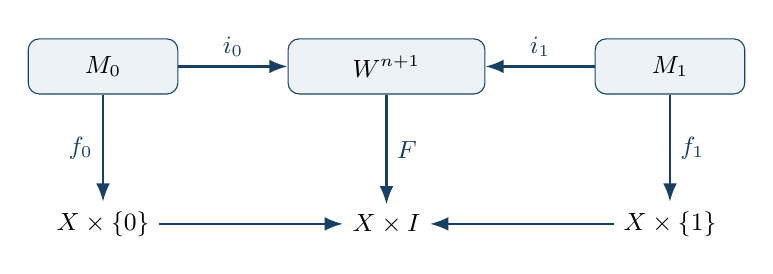
\begin{tikzpicture}[>=Latex,font=\small,
 every node/.style={align=center}]
 \node[draw=manifoldblue!75!black,fill=manifoldblue!8,
   rounded corners,minimum width=1.9cm,minimum height=.7cm]
   (m0) at (0,2) {$M_0$};
 \node[draw=manifoldblue!75!black,fill=manifoldblue!8,
   rounded corners,minimum width=2.5cm,minimum height=.7cm]
   (w) at (3.6,2) {$W^{n+1}$};
 \node[draw=manifoldblue!75!black,fill=manifoldblue!8,
   rounded corners,minimum width=1.9cm,minimum height=.7cm]
   (m1) at (7.2,2) {$M_1$};
 \node (x0) at (0,0) {$X\times\{0\}$};
 \node (xi) at (3.6,0) {$X\times I$};
 \node (x1) at (7.2,0) {$X\times\{1\}$};
 \draw[->,thick,manifoldblue!70!black]
   (m0)--node[above] {$i_0$} (w);
 \draw[<-,thick,manifoldblue!70!black]
   (w)--node[above] {$i_1$} (m1);
 \draw[->,thick,manifoldblue!70!black]
   (m0)--node[left] {$f_0$} (x0);
 \draw[->,thick,manifoldblue!70!black]
   (w)--node[right] {$F$} (xi);
 \draw[->,thick,manifoldblue!70!black]
   (m1)--node[right] {$f_1$} (x1);
 \draw[->,thick,manifoldblue!70!black]
   (x0)--(xi);
 \draw[<-,thick,manifoldblue!70!black]
   (xi)--(x1);
\end{tikzpicture}
\caption{Normalny ślad nad cylindrem $X\times I$.
Dolny brzeg $M_0$ jest daną początkową,
górny $M_1$ wynikiem działania. Przy lewej
strzałce $\theta_{n+1}$ oba końce są ustalone
jako $X$; przy działaniu $L_{n+1}^s$
górny koniec może się zmienić.}
\label{fig:surgery-cobordism-cylinder-23}
\end{figure}

W rysunku strzałki poziome są inkluzjami
brzegów, a kwadraty komutują z dokładnością
do homotopii zgodnej z danymi normalnymi.
Przy $\eta(s_0)=\eta(s_1)$ istnieje taki
normalny ślad między strukturami.
Jego przeszkoda określa element przenoszący
$s_0$ w $s_1$, więc włókno $\eta$ jest orbitą.
Gdy oba końce reprezentują punkt wyróżniony,
możemy wybrać dyfeomorfizm identyfikujący
górną strukturę z $(X,\id_X)$.
Utożsamienie takiego śladu z normalną daną
cylindra i odwrotna implikacja są treścią
Twierdzenia 10.8 Walla: obraz $\theta_{n+1}$
jest dokładnie stabilizatorem bazy.

\clearpage
\section{Wersja z ustalonym brzegiem}
\label{sec:relative-surgery-23}
\index{ciag dokladny chirurgii@Ciąg dokładny chirurgii!wersja z ustalonym brzegiem@wersja z ustalonym brzegiem}

Niech teraz $X^n$ będzie zwartą, spójną,
gładką rozmaitością wymiaru $n\geq5$
z niepustym brzegiem. Ustalamy jego
gładką strukturę i identyfikację brzegu
każdej rozważanej rozmaitości z $\partial X$.
Przez $\mathcal S^s_{\mathrm{DIFF}}(X\operatorname{rel}\partial X)$
rozumiemy klasy prostych równoważności par
$f:(M,\partial M)\to(X,\partial X)$,
których ograniczenie do brzegu jest tą
ustaloną dyfeomorficzną identyfikacją.
Równoważność par wymaga dyfeomorfizmu
zgodnego z nią na brzegu i homotopii
odwzorowań ustalonej na brzegu.
Normalne odwzorowania i ich kobordyzmy
mają na kołnierzu brzegu dane produktowe.
Stopień jeden rozumiemy względem
względnych klas fundamentalnych:
$f^*w_X=w_M$ oraz
$f_*[M,\partial M]=[X,\partial X]$
w $H_n(X,\partial X;\Z^{w_X})$.
Intuicja jest taka sama jak poprzednio,
ale żadna chirurgia nie zmienia już
zadanej gładkiej struktury na $\partial X$.

\begin{twierdzenie}[Ciąg chirurgii z ustalonym brzegiem;
 wynik zewnętrzny]
\label{thm:relative-surgery-23}
Niech $\pi=\pi_1(X)$, a $w$ będzie jego
charakterem orientacji. Przy powyższych
hipotezach i konwencji o ustalonym brzegu,
jeśli $Q=X/\partial X$, istnieje ciąg
zbiorów z punktami wyróżnionymi
\begin{equation}\label{eq:relative-surgery-23}
 [\Sigma Q,G/O]\xrightarrow{\ \theta_{n+1}^{\mathrm{rel}}\ }
 L_{n+1}^s(\Z[\pi],w)
 \xrightarrow{\ \partial_{\!s}^{\mathrm{rel}}\ }
 \mathcal S^s_{\mathrm{DIFF}}(X\operatorname{rel}\partial X)
 \xrightarrow{\ \eta^{\mathrm{rel}}\ }
 [Q,G/O]
 \xrightarrow{\ \theta_n^{\mathrm{rel}}\ }
 L_n^s(\Z[\pi],w).
\end{equation}
Dokładność ma to samo znaczenie orbit,
stabilizatora i przeciwobrazu zera co
w Twierdzeniu~\ref{thm:exact-surgery-23}.
Nie zakładamy, by inkluzje składowych
brzegu indukowały izomorfizmy grup
podstawowych.
\end{twierdzenie}

Iloraz $Q$ zapamiętuje warunek na brzegu:
odwzorowania $X\to G/O$ wysyłające
$\partial X$ w punkt bazowy, z homotopiami
ustalonymi na $\partial X$, odpowiadają
opartym odwzorowaniom $Q\to G/O$.
Analogicznie normalne dane na $X\times I$
ustalone na $X\times\partial I$ i
$\partial X\times I$ są klasyfikowane przez
$[\Sigma Q,G/O]$. Ściana $\partial X\times I$
na rysunku~\ref{fig:surgery-cobordism-cylinder-23}
pozostaje wtedy cylindrem produktowym.
Wyniki z
\href{https://webhomes.maths.ed.ac.uk/~v1ranick/books/scm.pdf}
{§10 książki Walla, \emph{Surgery on Compact Manifolds}},
w tym gładki odpowiednik Twierdzenia 10.8,
dają identyfikację danych normalnych,
kryterium realizacji, działanie i dokładność
również w tej wersji. To są użyte tu
wyniki zewnętrzne, a nie wniosek wyłącznie
z zastąpienia $X$ przez $Q$ w poprzednim wzorze.

\begin{przyklad}[Dysk z ustalonym brzegiem]
Dla $X=D^n$ mamy $Q=D^n/S^{n-1}\cong S^n$.
Względne dane normalne są więc klasami
$[S^n,G/O]=\pi_n(G/O)$, a dane cylindra
klasami $\pi_{n+1}(G/O)$.
To pokazuje, dlaczego warunek na brzegu
jest istotny: bez niego $[D^n,G/O]$
ma tylko klasę stałą.
Przykład identyfikuje dane wejściowe ciągu;
nie oblicza jeszcze jego zbioru struktur.
\end{przyklad}

\section{Co ciąg mówi w praktyce?}
\label{sec:applications-surgery-23}

\begin{przyklad}[Cel po prostu spójny]
\label{prz:simply-connected-surgery-23}
Gdy $\pi=1$, obliczenie z
Sekcji~\ref{sec:obliczenia-LZ-22} daje
\[
 L_{4j}^s(\Z)\cong\Z,\qquad
 L_{4j+2}^s(\Z)\cong\Z/2,\qquad
 L_{2j+1}^s(\Z)=0.
\]
W wymiarze $4j$ pierwsza przeszkoda
normalnego odwzorowania jest sygnaturą
formy jądra podzieloną przez $8$.
Rozszczepienie z
Lematu~\ref{lem:split-normalne-21}
jest ortogonalne dla przecięć. Oznaczmy przez
$K=\ker\bigl(f_*:H_{2j}(M;\Q)\to
H_{2j}(X;\Q)\bigr)$. Dla $y\in K$
i $x\in H_{2j}(X;\Q)$
naturalność przecięć daje
$\lambda_M(f_!x,y)=\lambda_X(x,f_*y)=0$.
Dlatego sygnatura jądra to
$\operatorname{sign}(M)-\operatorname{sign}(X)$.
W wymiarze $4j+2$ mierzy ją
niezmiennik Arfa formy kwadratowej.
W wymiarach nieparzystych grupa przeszkód
jest zerowa. W każdym z tych przypadków
ciąg nadal wymaga obliczenia $[X,G/O]$
oraz działania $L_{n+1}$, zanim
rozróżnimy wszystkie struktury.
\end{przyklad}

\clearpage
\begin{przyklad}[Ślad sfery i produktu w ciągu chirurgii]
\label{prz:slad-s6-ciag-23}
Niech $W$ i $(f,b):M=S^3\times S^3\to S^6$
będą śladem i jego górną mapą normalną z
Przykładu~\ref{prz:slad-s6-produkt-21}.
Od strony $S^6$ ślad ma uchwyt indeksu trzy;
od strony $M$ uchwyt indeksu cztery na
$B=\{0\}\times S^3$ w nowo dołączonej
połowie $D^3\times S^3$ przywraca $S^6$.
To ta sama operacja oglądana z dwóch końców.

Połóżmy $A=S^3\times\{*\}$. Ponieważ
$H_3(S^6)=0$, jądro górnej mapy jest
$K_3(f)=H_3(M)=\Z[A]\oplus\Z[B]$.
Przykład~\ref{prz:forma-produkt-21} oblicza
$\lambda(A,B)=1$ oraz
$\lambda(A,A)=\lambda(B,B)=0$.
Lemat~\ref{lem:wall-lokalna-stabilizacja-22}
oraz Przykład~\ref{prz:produkt-L-22} dają
$\mu(A)=\mu(B)=0$ dla standardowego wyboru
$b$ w tym śladzie. Zatem dla
$\bar x,\bar y\in\mathbb F_2$ funkcja
kwadratowa ma postać
\[
 q(\bar x[A]+\bar y[B])=\bar x\bar y,
 \qquad \operatorname{Arf}(q)=0.
\]
Według rachunku z
Sekcji~\ref{sec:obliczenia-LZ-22}
przeszkoda tej mapy jest więc zerem
w $L_6^s(\Z)\cong\Z/2$.

Normalny ślad $W$ łączy $(f,b)$ z
$(S^6,\id_{S^6})$. Dlatego klasa normalna
$a=[f,b]\in[S^6,G/O]$ jest punktem wyróżnionym:
$a=0$. W ciągu~\eqref{eq:exact-surgery-23}
otrzymujemy konkretnie
\[
 [S^6,\id_{S^6}]
 \xrightarrow{\ \eta\ }a=0
 \xrightarrow{\ \theta_6\ }0\in L_6^s(\Z).
\]
Ponieważ $L_7^s(\Z)=0$ z~\eqref{eq:L-Z-22},
opis orbit w
Twierdzeniu~\ref{thm:exact-surgery-23} mówi,
że standardowa sfera jest jedyną strukturą
w tym włóknie $\eta$.
Sama mapa $f$ nie jest elementem zbioru
struktur: jej jądro $K_3(f)$ ma rangę dwa,
więc $f$ nie jest równoważnością homotopijną.
Wniosek $a=0$ korzysta z konkretnych danych
normalnych wybranych przez $W$.
\end{przyklad}

\begin{stwierdzenie}[Sfery homotopijne jako struktury nad $S^7$]
\label{prop:structure-set-seven-sphere-23}
\index{zbior struktur@Zbiór struktur!sfera wymiaru siedem@sfera wymiaru siedem}
Istnieje bijekcja zbiorów z punktami wyróżnionymi
\[
 \mathcal S^s_{\mathrm{DIFF}}(S^7)\cong\Theta_7,
\]
gdzie $\Theta_7$ oznacza zorientowane klasy
dyfeomorfizmu gładkich sfer homotopijnych.
\end{stwierdzenie}
\begin{proof}
Ustalmy orientację $S^7$.
Para $(M,f)$ ze zbioru struktur nadaje $M$
orientację, dla której $f:M\to S^7$ ma stopień
$+1$. Ponieważ $f$ jest równoważnością
homotopijną, $M$ jest sferą homotopijną.
Odwrotnie każda zorientowana sfera homotopijna
ma równoważność homotopijną stopnia $+1$
z $S^7$. Jest ona prosta, bo $\pi_1(S^7)=1$
i $\operatorname{Wh}(1)=0$.
Dwie mapy stopnia $+1$ z tej samej
siedmiowymiarowej sfery homotopijnej
do $S^7$ są homotopijne: ponieważ $S^7$
jest $6$-spójna, klasy takich map z
siedmiowymiarowego kompleksu CW
wyznacza stopień. Wobec tego zgodność
orientacji przy dyfeomorfizmie dokładnie
odpowiada równoważności par ze zbioru
struktur. Klasa $S^7$ odpowiada punktowi
wyróżnionemu.
\end{proof}

Twierdzenie~\ref{thm:all-seven-spheres-25}
podaje $28$ elementów $\Theta_7$, w tym
klasy sum spójnych sfery Milnora $M_3$.
To daje konkretną interpretację zbioru
struktur w ciągu~\eqref{eq:exact-surgery-23}.
Liczba $28$ wynika tam z wyników
Kervaire'a--Milnora i Eellsa--Kuipera;
niniejszy rozdział nie oblicza obrazu
lewej strzałki $\theta_8$ i nie wyprowadza
tej liczby z samego ciągu.

\begin{przyklad}[Dlaczego zerowa przeszkoda
nie oznacza jedynej struktury]
\label{prz:nonunique-structure-23}
Dla $\theta_n(a)=0$ istnieje
\emph{co najmniej jedna} prosta równoważność
o normalnej klasie $a$. Wszystkie
struktury z tą klasą tworzą jedną orbitę
$L_{n+1}^s$, która może zawierać
więcej niż jeden element.
To jest algebraiczne miejsce na różne
gładkie realizacje tego samego typu
homotopijnego. Sfery Milnora z
Rozdziału~\ref{ch:sfery-Milnora}
dadzą konkretny powód, dla którego
samej równoważności homotopijnej
nie wolno utożsamiać z dyfeomorfizmem.
\end{przyklad}

\noindent\textbf{Granica tej części.}
Ciąg~\eqref{eq:exact-surgery-23} kończy
program \emph{wysokowymiarowej} chirurgii
w sensie logicznym: podaje kryterium
istnienia struktury i opis niejednoznaczności.
Nie jest automatyczną tabelą dyfeomorfizmów.
Do obliczenia konkretnego $\mathcal S^s(X)$
potrzeba znać homotopie $G/O$, grupy $L$
danego pierścienia grupowego i działanie
poprzedniej grupy. W niższych wymiarach
podane hipotezy twierdzeń Walla i
$s$-kobordyzmu nie są spełnione.

\par\smallskip
{\footnotesize\noindent\emph{Dalsza lektura:}
\href{https://webhomes.maths.ed.ac.uk/~v1ranick/books/scm.pdf}
{C.~T.~C. Wall, \emph{Surgery on Compact Manifolds}, §10.2--10.8},
\href{https://www.maths.ed.ac.uk/~v1ranick/surgery/ranicki.pdf}
{A.\ Ranicki, \emph{An Introduction to Algebraic Surgery},
część o ciągu dokładnym chirurgii}.\par}

\clearpage

\chapter{Twierdzenie Poincarégo w wymiarze dwa i w wysokich wymiarach}
\label{ch:poincare-2-high}
\index{twierdzenie Poincarego@Twierdzenie Poincarégo}

Twierdzenie Poincarégo pyta, kiedy rozmaitość
o typie homotopijnym sfery musi być sferą.
W rozdziale o chirurgii widzieliśmy już,
że \emph{homeomorfizm} i \emph{dyfeomorfizm}
to różne wymagania. Sformułujemy tu
wniosek topologiczny dla powierzchni
i dla gładkich sfer homotopijnych
wymiaru co najmniej pięć.

\begin{definicja}[Sfera homotopijna]
\index{sfera homotopijna@Sfera homotopijna}
\label{def:homotopy-sphere-24}
Zamknięta, spójna rozmaitość $n$-wymiarowa
$\Sigma^n$ jest \emph{sferą homotopijną},
jeśli $\Sigma\simeq S^n$.
Na przykład standardowa $S^n$ spełnia
ten warunek. Definicja nie zawiera
stwierdzenia o dyfeomorfizmie.
\end{definicja}

\section{Powierzchnie: klasyfikacja i konsekwencja}
\label{sec:poincare-2}

\begin{twierdzenie}[Klasyfikacja zamkniętych powierzchni]
\label{thm:classification-surfaces-24}
Każda spójna, zwarta powierzchnia
bez brzegu jest homeomorficzna
dokładnie z jednym modelem z listy:
$S^2$, suma spójna $g\geq1$ torusów
albo suma spójna $h\geq1$ płaszczyzn
rzutowych $\mathbb{RP}^2$.
W pierwszej rodzinie charakterystyka
Eulera wynosi $2-2g$, w drugiej $2-h$;
orientowalność odróżnia rodziny.
\end{twierdzenie}

\begin{proof}
Jedynym wynikiem wejściowym o powierzchniach
jest ich \emph{triangulowalność}: zwarta
topologiczna powierzchnia ma skończoną
triangulację. Dla powierzchni gładkich jest
to twierdzenie Cairnsa przytoczone w
Dodatku~\ref{app:wyniki-zewnetrzne}.
\href{https://pi.math.cornell.edu/~hatcher/Papers/TorusTrick.pdf}
{A.\ Hatcher, \emph{The Kirby Torus Trick for Surfaces}}
wykazuje wygładzalność powierzchni topologicznych;
połączenie obu wyników daje potrzebną tutaj
triangulację topologiczną.
Pozostałe kroki rozpiszemy. Oznaczmy przez
$v,e,t$ liczby wierzchołków, krawędzi
i trójkątów wybranej triangulacji $F$.

\emph{Krok 1: charakterystyka i sfera.}
W szkielecie jednowymiarowym wybierzmy
drzewo rozpinające $T$. Jego małe regularne
otoczenie jest dyskiem: zaczynamy od dysku
przy jednym wierzchołku, a każda następna
krawędź drzewa dokleja prostokątny pas
do dotychczasowego dysku wzdłuż jednego łuku.
W szczególności $T$ nie rozcina $F$;
ścieżkę przecinającą $T$ można poprowadzić
wzdłuż brzegu tego otoczenia.

Niech $D$ będzie grafem dualnym z wierzchołkiem
w każdym trójkącie i krawędzią przecinającą
każdą krawędź triangulacji \emph{spoza} $T$.
Jest spójny: przechodząc między trójkątami
w $F\setminus T$, możemy omijać krawędzie
$T$, więc kolejne przejścia dają drogę w $D$.
Graf $T$ ma $v$ wierzchołków i $v-1$ krawędzi,
a $D$ ma $t$ wierzchołków i $e-(v-1)$ krawędzi.
Stąd, pisząc $b_1(D)=|E(D)|-|V(D)|+1$,
otrzymujemy
\[
 \chi(F)=v-e+t=1+\chi(D)=2-b_1(D)\leq 2.
\]
Jeżeli $\chi(F)=2$, to $D$ jest drzewem.
Pogrubienia obu drzew są dyskami;
prostokąty wzdłuż krawędzi triangulacji
spoza $T$ wypełniają obszar między ich
brzegami. Dają zatem rozkład $F$ na dwa
dyski sklejone całymi brzegami, czyli
$F\cong S^2$. Odwrotna implikacja wynika
z $\chi(S^2)=2$.

Jeżeli $\chi(F)<2$, graf $D$ zawiera prosty
cykl $\gamma$. Jest on \emph{nierozdzielający}:
$F\setminus D$ jest spójne, bo każdy punkt
można połączyć w swoim trójkącie z wierzchołkiem
triangulacji, a wszystkie te wierzchołki łączy
$T\subset F\setminus D$. Zatem również
$F\setminus\gamma$ jest spójne.

\emph{Krok 2: cięcie i zmiana $\chi$.}
Prosta zamknięta krzywa ma regularne otoczenie
będące pierścieniem albo wstęgą Möbiusa.
Rozcięcie wzdłuż krzywej nie zmienia
charakterystyki Eulera: zarówno jej
otoczenie, jak i okręgi wspólnego brzegu
mają $\chi=0$, więc wzór na $\chi$ sumy
powierzchni daje $\chi(F)=\chi(F\setminus
\operatorname{int}N(\gamma))$.
Zamknięcie każdej nowej składowej brzegu
dyskiem zwiększa $\chi$ o jeden.
W przypadku krzywej dwustronnej są dwa
okręgi brzegowe; w przypadku jednostronnej
jest jeden. Krzywa jednostronna nie rozdziela
$F$, gdyż dopełnienie jej wstęgi Möbiusa
ma tylko jeden okrąg brzegowy.

\emph{Krok 3: powierzchnie orientowalne.}
Indukujemy po $r=2-\chi(F)$. Dla $r=0$
mamy sferę z Kroku 1. Jeśli $F$ jest
orientowalna i $r>0$, wybieramy powyższy
nierozdzielający cykl $\gamma$. Jest dwustronny.
Po rozcięciu i zamknięciu obu brzegów
dostajemy spójną orientowalną powierzchnię
$F'$ o $\chi(F')=\chi(F)+2$.
Z założenia indukcyjnego $F'\cong\#^gT^2$
dla pewnego $g\geq0$. Aby odzyskać $F$,
usuwamy z $F'$ wnętrza dwóch dysków i
łączymy ich brzegi pierścieniem.
Zgodność orientacji wymusza zwykły
uchwyt; jest to dokładnie operacja
$F\cong F'\#T^2$ opisana w
Przykładzie~\ref{prz:sfera-torus-chirurgia-18}.
Zatem $F\cong\#^{g+1}T^2$.

\emph{Krok 4: powierzchnie nieorientowalne.}
Istnieje na $F$ zamknięta droga odwracająca
orientację. Po ustawieniu jej w położeniu
ogólnym wybieramy taką drogę z najmniejszą
liczbą samoprzecięć. W każdym podwójnym
punkcie wygładzenie rozcina drogę na dwie;
iloczyn ich znaków zmiany orientacji jest
równy $-1$, więc jedna z nich także odwraca
orientację. Wybierając ją, zmniejszamy
liczbę samoprzecięć. W końcu otrzymujemy
prostą krzywą jednostronną $\delta$.
Po rozcięciu wzdłuż $\delta$ i zamknięciu
jedynego brzegu dyskiem powstaje spójna
powierzchnia $F'$ z $\chi(F')=\chi(F)+1$.
Odwrotnie, $F\cong F'\#\mathbb{RP}^2$,
bo zastępujemy ten dysk wstęgą Möbiusa.

Jeżeli $F'$ jest nieorientowalna, indukcja
daje $F'\cong\#^h\mathbb{RP}^2$, a więc
$F\cong\#^{h+1}\mathbb{RP}^2$.
Jeżeli $F'$ jest orientowalna, to
$F\cong(\#^gT^2)\#\mathbb{RP}^2$.
Przy $g=0$ dostajemy $\mathbb{RP}^2$.
Przy $g>0$ stosujemy lokalne przesunięcie
wstęg
\begin{equation}\label{eq:crosscap-handle-24}
 T^2\#\mathbb{RP}^2
 \cong\mathbb{RP}^2\#\mathbb{RP}^2
       \#\mathbb{RP}^2.
\end{equation}
Aby sprawdzić tę relację, przedstawmy
lewą stronę jako dysk z trzema pasami:
dwa nieskręcone pasy torusa mają końce
ułożone naprzemiennie, trzeci pas ma
półobrót i daje płaszczyznę rzutową.
Brzeg wielokąta opisuje słowo
$aba^{-1}b^{-1}cc$. Użyjemy elementarnego
przekształcenia
\[
 xUxV\ \sim\ U^{-1}xxV.
\]
Obie litery $x$ oznaczają boki sklejane
w tym samym kierunku. Rozcinamy wielokąt
wzdłuż łuku łączącego te boki i sklejamy
go po drugiej stronie pary: boki $x$
stają obok siebie, a odcinek brzegu $U$
jest teraz obchodzony w odwrotnym kierunku.
Iloraz powierzchni się nie zmienia.
Wolno też cyklicznie przesuwać słowo
brzegowe i zastępować nazwę boku
jej odwrotnością. Stosując tę regułę
cztery razy, dostajemy jawnie
\[
\begin{aligned}
 aba^{-1}b^{-1}cc
 &\sim aba^{-1}cbc
  \sim abbc^{-1}ac\\
 &\sim aacb^{-1}b^{-1}c
  \sim aabbcc.
\end{aligned}
\]
Końcowe trzy pary boków są skręcone,
więc wyznaczają sumę spójną trzech
$\mathbb{RP}^2$, co dowodzi~\eqref{eq:crosscap-handle-24}.
Ten sam rachunek słów zapisuje
\href{https://pnp.mathematik.uni-stuttgart.de/igt/eiserm/lehre/Topologie/Topologie-K-2x2.pdf}
{M.\ Eisermann, \emph{Topologie}, twierdzenie K3f (8)};
diagram geometryczny podaje
\href{https://www.math.uchicago.edu/~may/VIGRE/VIGRE2008/REUPapers/Huang.pdf}
{J.\ Huang, \emph{Classification of Surfaces}, rys.~13}.
Stosując~\eqref{eq:crosscap-handle-24}
$g$ razy, otrzymujemy sumę spójną
$(2g+1)$ płaszczyzn rzutowych.

Pozostaje jednoznaczność. Dodawanie torusa
zmniejsza $\chi$ o dwa, a dodawanie
$\mathbb{RP}^2$ o jeden, gdyż
$\chi(A\#B)=\chi(A)+\chi(B)-2$.
Tak dostajemy podane w tezie wzory.
Obie rodziny rozróżnia orientowalność,
a wewnątrz każdej rodziny wartość $\chi$
wyznacza liczbę składników. Charakterystyka
jest niezmiennikiem topologicznym, ponieważ
równa się naprzemiennej sumie rang homologii
singularnych z Dodatku~\ref{app:homologia-singularna-euler}.
\end{proof}

W powyższym dowodzie zewnętrzne jest tylko
twierdzenie o triangulacji powierzchni.
Krótki wariant argumentu dla powierzchni
orientowalnych podaje
\href{https://academicweb.nd.edu/~andyp/notes/ClassificationSurfaces.pdf}
{A.\ Putman, \emph{A Quick Proof of the Classification of Surfaces}};
pełniejszą wersję obu przypadków zawierają
\href{https://academicweb.nd.edu/~andyp/notes/ClassificationSurfacesLong.pdf}
{jego notatki, §5--6}.

\begin{lemat}[Pierwsza homologia modeli]
\label{lem:H1-surfaces-24}
Dla $g,h\geq1$ mamy
\[
 H_1(\#^g T^2;\Z)\cong\Z^{2g},
 \qquad
 H_1(\#^h\mathbb{RP}^2;\Z)
     \cong\Z^{h-1}\oplus\Z/2.
\]
\end{lemat}
\begin{proof}
Standardowy wielokąt orientowalnej
powierzchni ma kolejno oznaczone boki
\[
a_1,b_1,a_1^{-1},b_1^{-1},\ldots,
a_g,b_g,a_g^{-1},b_g^{-1}.
\]
Po sklejeniu dostajemy jedną komórkę
zerową, $2g$ komórek jednowymiarowych
i jedną dwuwymiarową. Operator brzegu
$\partial_1$ jest zerowy, bo oba końce
każdej krawędzi to ten sam wierzchołek.
W brzegowym słowie komórki dwuwymiarowej
każda krawędź pojawia się raz z plusem
i raz z minusem, więc $\partial_2=0$.
Zatem $H_1=\ker\partial_1/
\operatorname{im}\partial_2=\Z^{2g}$.

Nieorientowalny wielokąt ma słowo
$a_1a_1\cdots a_ha_h$. Teraz
$C_1\cong\Z^h$, $\partial_1=0$,
a $\partial_2(1)=2(a_1+\cdots+a_h)$.
Wektor $(1,\ldots,1)$ jest prymitywny
w $\Z^h$, więc można go uzupełnić do
bazy całkowitej. W tej bazie iloraz
przez podgrupę generowaną przez jego
podwojenie jest
$\Z^{h-1}\oplus\Z/2$.
\end{proof}

\begin{twierdzenie}[Twierdzenie Poincarégo dla powierzchni]
\label{thm:poincare-2-24}
Każda spójna, zamknięta powierzchnia
homotopijnie równoważna $S^2$
jest homeomorficzna z $S^2$.
Równoważnie: jedyną spójną, zamkniętą
i po prostu spójną powierzchnią
jest $S^2$.
\end{twierdzenie}
\begin{proof}
Równoważność homotopijna zachowuje
homologię, więc $H_1(\Sigma;\Z)=
H_1(S^2;\Z)=0$.
Twierdzenie~\ref{thm:classification-surfaces-24}
ogranicza $\Sigma$ do trzech rodzin.
Lemat~\ref{lem:H1-surfaces-24}
wyklucza wszystkie modele o $g\geq1$
i $h\geq1$, ponieważ każda z ich
grup $H_1$ jest niezerowa.
Pozostaje tylko $S^2$.
Jeśli założymy zamiast równoważności
homotopijnej prostą spójność, to
$H_1(\Sigma;\Z)$ jest abelianizacją
$\pi_1(\Sigma)$, więc ten sam argument
daje identyczny wniosek.
\end{proof}

\section{Usunięcie dwóch dysków ze sfery homotopijnej}
\label{sec:poincare-high}

Następny argument dotyczy \emph{gładkiej}
sfery homotopijnej $\Sigma^n$.
Wybierzmy dwa rozłączne gładko
zanurzone zamknięte dyski $D_-^n,D_+^n$
i połóżmy
\[
 W=\Sigma\setminus
   \bigl(\operatorname{int}D_-^n
          \sqcup\operatorname{int}D_+^n\bigr),
 \qquad
 \partial W=S_-^{n-1}\sqcup S_+^{n-1}.
\]
Przestrzeń $W$ jest kobordyzmem,
którego dwiema składowymi brzegu
są sfery standardowe.

\begin{lemat}[Dlaczego to $h$-kobordyzm?]
\label{lem:punctured-sphere-hc-24}
Jeżeli $n\geq3$ i $\Sigma^n\simeq S^n$,
to obie inkluzje
$S_\pm^{n-1}\hookrightarrow W$
są równoważnościami homotopijnymi.
\end{lemat}
\begin{proof}
Przez wycinanie para $(\Sigma,W)$
ma tę samą homologię względną
co suma dwóch par $(D^n,S^{n-1})$.
Jej jedyną niezerową grupą względną
w dodatnim stopniu jest zatem
$H_n(\Sigma,W)\cong\Z\oplus\Z$.
Fragment długiego ciągu ma postać
\[
 0\longrightarrow H_n(\Sigma)\cong\Z
 \xrightarrow{\ (1,1)\ }
 \Z\oplus\Z
 \xrightarrow{\ \partial\ }
 H_{n-1}(W)\longrightarrow0.
\]
Znaki obu współrzędnych zależą od
orientacji dysków; wybieramy je tak,
aby pierwsza strzałka była diagonalna.
Stąd $H_{n-1}(W)\cong\Z$, a obrazy
obu wektorów bazowych przez $\partial$
są jej generatorami z przeciwnymi znakami.
Są to klasy fundamentalne obu składowych
brzegu. Pozostałe grupy zredukowane
$H_i(W)$ znikają, jak dla $S^{n-1}$.

Przez twierdzenie van Kampena,
usunięcie wnętrza każdego $n$-dysku
nie zmienia $\pi_1$ dla $n\geq3$:
część wspólna w odpowiednim otwartym
rozkładzie deformuje się na
$S^{n-1}$ i jest po prostu spójna.
Zatem $\pi_1(W)\cong\pi_1(\Sigma)=1$.
Obie sfery brzegowe też są po prostu
spójne. Ich inkluzje są izomorfizmami
homologii, więc homologiczną wersją
twierdzenia Whiteheada
(Wniosek~\ref{cor:whitehead-homologiczny})
są równoważnościami homotopijnymi.
\end{proof}

\begin{figure}[htbp]
\centering
\begin{tikzpicture}[>=Latex,font=\small,line cap=round]
 \shade[inner color=white,outer color=manifoldblue!43]
      (0,0) circle (1.55);
 \draw[manifoldblue!75!black,very thick]
      (0,0) circle (1.55);
 \fill[white] (-1.02,.70) circle (.27);
 \fill[white] (1.02,-.70) circle (.27);
 \draw[manifoldgold!80!black,thick]
      (-1.02,.70) circle (.27)
      (1.02,-.70) circle (.27);
 \node[anchor=east,align=right] at (-1.42,1.15)
      {$D_-^n$\\usunięty};
 \node[anchor=west,align=left] at (1.42,-1.13)
      {$D_+^n$\\usunięty};
 \draw[->,very thick,manifoldblue!70!black]
      (2.05,0)--(3.15,0);
 \draw[manifoldblue!75!black,very thick,
       fill=manifoldblue!12]
      (3.52,-1.07) rectangle (6.82,1.07);
 \draw[manifoldgold!85!black,very thick]
      (3.52,-1.07)--(3.52,1.07)
      (6.82,-1.07)--(6.82,1.07);
 \node at (5.17,.34) {$W$};
 \node at (3.52,-1.40) {$S_-^{n-1}$};
 \node at (6.82,-1.40) {$S_+^{n-1}$};
\end{tikzpicture}
\caption{Schemat wycięcia dwóch dysków z $\Sigma^n$.
Prostokąt przedstawia kobordyzm po zastosowaniu
twierdzenia o $h$-kobordyzmie; dla $n\geq6$
jest on gładkim iloczynem. Rysunek jest
schematyczny, nie jest zanurzeniem $\Sigma^n$
w płaszczyźnie.}
\label{fig:poincare-two-disks-24}
\end{figure}

\begin{twierdzenie}[Poincaré dla gładkich
sfer homotopijnych, $n\geq6$]
\label{thm:poincare-high-24}
Jeżeli $\Sigma^n$ jest gładką sferą
homotopijną i $n\geq6$, to
$\Sigma$ jest homeomorficzna z $S^n$.
\end{twierdzenie}
\begin{proof}
Lemat~\ref{lem:punctured-sphere-hc-24}
mówi, że $(W;S_-^{n-1},S_+^{n-1})$
jest po prostu spójnym $h$-kobordyzmem.
Jego wymiar wynosi $n$, zatem $n\geq6$
pozwala użyć gładkiego twierdzenia
Smale'a o $h$-kobordyzmie
(Twierdzenie~\ref{thm:smale-hc-19}).
Otrzymujemy dyfeomorfizm
$W\cong S^{n-1}\times[0,1]$
ustalony na dolnym brzegu.
Po ponownym doklejeniu dwóch dysków
powstaje przestrzeń
$D^n\cup_{\varphi}D^n$
dla pewnego dyfeomorfizmu
$\varphi:S^{n-1}\to S^{n-1}$.
Każdy taki $\varphi$ ma \emph{ciągłe}
przedłużenie na dysk dane wzorem
$r u\mapsto r\varphi(u)$ dla
$0\leq r\leq1$, $u\in S^{n-1}$;
w środku kładziemy $0\mapsto0$.
Wzór odwrotny pochodzi od
$\varphi^{-1}$, więc jest to
homeomorfizm dysków. Zmieniając
nim parametryzację jednego dysku,
uzyskujemy homeomorfizm
$D^n\cup_\varphi D^n\cong
D^n\cup_{\id}D^n\cong S^n$.
Stożkowe przedłużenie nie musi
być gładkie w środku dysku;
dlatego dowód daje homeomorfizm,
a nie dyfeomorfizm.
\end{proof}

\section{Osobny przypadek wymiaru pięć}
\label{sec:poincare-five}

Dla $n=5$ kobordyzm $W$ z poprzedniej
sekcji ma wymiar $5$, podczas gdy
Twierdzenie~\ref{thm:smale-hc-19}
wymaga wymiaru kobordyzmu co najmniej $6$.
Nie wolno zastosować go tutaj przez
samą zmianę numeru wymiaru.
Można jednak bez klasyfikacji rozpoznać
topologię sfery po wyjęciu \emph{jednego}
dysku; ujawnia to dokładnie brakujący krok.

\begin{lemat}[Co daje wyjęcie jednego dysku]
\label{lem:punctured-five-24}
Jeżeli $\Sigma^5\simeq S^5$ jest gładka
i $D^5\subset\Sigma$ jest gładko zanurzonym
dyskiem, to
$C=\Sigma\setminus\operatorname{int}D^5$
jest zwartą gładką rozmaitością
\emph{ściągalną} o brzegu dyfeomorficznym
z $S^4$.
\end{lemat}
\begin{proof}
Gładka tuba brzegu dysku daje rozkład
$\Sigma=C\cup D^5$ z częścią wspólną
o typie homotopijnym $S^4$.
W ciągu Mayera--Vietorisa homomorfizm
$H_5(\Sigma)\cong\Z\to H_4(S^4)\cong\Z$
jest izomorfizmem: wysyła klasę
fundamentalną na klasę brzegu dysku.
Z dokładności dostajemy $H_4(C)=0$,
a wszystkie pozostałe dodatnie grupy
homologii $C$ też znikają, ponieważ
$\Sigma$ ma homologię $S^5$.
Twierdzenie van Kampena daje
$\pi_1(C)=\pi_1(\Sigma)=1$,
gdyż $D^5$ i $S^4$ są po prostu spójne.
Rozmaitość ma typ kompleksu CW;
homologiczna wersja twierdzenia
Whiteheada zastosowana do
punktu $*\to C$ daje ściągalność.
Brzeg $C$ jest dokładnie
$\partial D^5\cong S^4$.
\end{proof}

Ściągalność $C$ nie daje jeszcze
dyfeomorfizmu $C\cong D^5$.
Takie wnioskowanie wymagałoby
oddzielnego twierdzenia o gładkich
wypełnieniach $S^4$. W następnym
argumencie korzystamy z klasyfikacji
zamkniętych $5$-rozmaitości Barden.
Przedstawimy oba twierdzenia klasyfikacyjne
Bardena wraz z ich dowodami i modelami.

\begin{twierdzenie}[Barden, twierdzenie 2.2]
\label{thm:Barden-5-24}
Niech $P,Q$ będą zamkniętymi, zorientowanymi,
gładkimi, po prostu spójnymi
$5$-rozmaitościami. Jeśli izomorfizm
$H_2(P;\Z)\to H_2(Q;\Z)$ zachowuje
formę wiązania na części torsyjnej
i klasy $w_2$, to pochodzi od
dyfeomorfizmu zachowującego orientację.
\end{twierdzenie}

Jest to
\href{https://www.sas.rochester.edu/mth/sites/doug-ravenel/otherpapers/barden.pdf}
{D.\ Barden, \emph{Simply Connected Five-Manifolds},
Ann. of Math. 82 (1965), twierdzenie 2.2}.
Przeprowadzimy dowód, rozdzielając
rachunek homologiczny od dwóch operacji
geometrycznych na kobordyzmie.

\subsection*{Forma wiązania i dane kobordyzmu}

Ponieważ $H_1(P;\Z)=0$, twierdzenie o
współczynnikach uniwersalnych identyfikuje
$H^2(P;\Z/2)$ z
$\operatorname{Hom}(H_2(P;\Z),\Z/2)$.
Tak będziemy odczytywać $w_2(P)$.
Na $T_P=\operatorname{Tor}H_2(P;\Z)$
forma wiązania
$b_P\colon T_P\times T_P\to\Q/\Z$
jest niezdegenerowana i antysymetryczna:
$b_P(x,y)=-b_P(y,x)$. Nie znaczy to,
że $b_P(x,x)=0$; z antysymetrii wynika
jedynie $b_P(x,x)\in\{0,1/2\}$.
W tym wymiarze zachodzi ponadto
\[
  2b_P(x,x)=0,\qquad
  b_P(x,x)=\tfrac12 w_2(P)(x)
  \quad(x\in T_P),
\]
gdzie $1\in\Z/2$ odpowiada $1/2\in\Q/\Z$.
Ostatnia równość, podobnie jak fakt,
że obecność niesparowanego składnika
$\Z/2$ wykrywa niezerową klasę
zorientowanego kobordyzmu, jest
\href{https://webhomes.maths.ed.ac.uk/~v1ranick/papers/kill.pdf}
{wynikiem Walla, \emph{Killing the Middle Homotopy Groups
of Odd Dimensional Manifolds}, stwierdzenia 1--2},
przytoczonym też jako lemat F u Bardena.
Potrzebna niżej klasyfikacja form wiązania
(Wall, lemat 4(ii)) daje bazę z parami
$(x_j,y_j)$ tego samego skończonego rzędu
$n_j$ i $b(x_j,y_j)=1/n_j$. Może też
wystąpić wyróżniona para $(z_1,z_2)$
rzędów $q,2q$, gdzie $q$ jest nieparzyste,
z $b(z_1,z_2)=1/q$ i $b(z_2,z_2)=1/2$;
dla $q=1$ pozostaje
pojedynczy składnik $\Z/2$. Uzupełniamy
te generatory bazą części wolnej $(e_k)$.
Można wybrać całą bazę tak, że $w_2$
jest niezerowe na najwyżej jednym elemencie
(Barden, lematy E i G). Zachowujemy
możliwe wartości $b(y_j,y_j)=1/2$;
ich pominięcie zepsułoby przypadek niespinowy.

Jeżeli $V^6$ jest zorientowanym kobordyzmem
od $P$ do $Q$, to jego brzeg jako
rozmaitość zorientowana jest
$N=P\sqcup(-Q)$. Dlatego
$b_N=b_P\oplus(-b_Q)$ na torsji
$H_2(N)=H_2(P)\oplus H_2(Q)$.
Oznaczmy przez $i_P,i_Q$ homomorfizmy
indukowane inkluzjami do $V$.
Dla $a\in H_2(P)$ różnica
$a-\varphi(a)$ oznacza element
$(a,-\varphi(a))\in H_2(N)$.

\begin{lemat}[Początkowy kobordyzm;
 Barden, lemat 3.1]
\label{lem:barden-start-24}
Przy założeniach Twierdzenia~\ref{thm:Barden-5-24}
istnieje zorientowany, po prostu spójny
kobordyzm $V^6$ od $P$ do $Q$ taki, że
\[
 H_2(V;\Z)=
 \begin{cases}
 0,&w_2(P)=w_2(Q)=0,\\
 \Z/2,&w_2(P)\ne0\ne w_2(Q).
 \end{cases}
\]
W drugim przypadku $w_2(V)$ jest
niezerowe na generatorze $H_2(V)$.
\end{lemat}
\begin{proof}
Najpierw trzeba wiedzieć, że $P$ i $Q$
są zorientowanie kobordantne.
Obliczenie Thoma daje
$\Omega^{SO}_5\cong\Z/2$, a jedyny
możliwy niezerowy charakterystyczny
licznik kobordyzmu w tym wymiarze to
$\langle w_2w_3,[P]\rangle$.
Lemat F Walla--Bardena wiąże tę liczbę
z niesparowanym składnikiem $\Z/2$
formy $b_P$. Izomorfizm $\varphi$
zachowuje $b$ i $w_2$, więc $P$ i $Q$
mają tę samą klasę w $\Omega^{SO}_5$.
Gdy obie są spin, używamy mocniejszego
obliczenia $\Omega^{Spin}_5=0$:
jednoznaczne struktury spin na jednospójnych
$P,Q$ ograniczają spinowy kobordyzm.
Oba obliczenia grup kobordyzmu są tu
wynikami zewnętrznymi. Podaje je
\href{https://www.sas.rochester.edu/mth/sites/doug-ravenel/otherpapers/barden.pdf}
{Barden, §0.4}, powołując się
odpowiednio na Thoma (1954) i
Nowikowa (1963).

Wybierzmy taki początkowy kobordyzm.
Chirurgiami na zanurzonych okręgach we
wnętrzu usuwamy generatory jego $\pi_1$.
W zorientowanym $6$-wymiarowym otoczeniu
normalna wiązka okręgu rzędu pięć jest
trywialna. W przypadku spin dobieramy
obramowanie zgodne ze strukturą spin.
Powstały kobordyzm jest jednospójny.
Twierdzenie Hurewicza daje
$\pi_2(V)\cong H_2(V;\Z)$; każdą
wybraną klasę reprezentuje zanurzona
$2$-sfera, bo w wymiarze sześć mapę
$S^2\to V$ można poprawić położeniem
ogólnym do injektywnej immersji,
a zwartość $S^2$ czyni ją zanurzeniem.
Jej orientowana
wiązka normalna rzędu cztery jest
trywialna dokładnie wtedy, gdy
$w_2(V)$ zeruje się na tej klasie:
wiązki nad $S^2$ klasyfikuje
$\pi_1(SO(4))\cong\Z/2$.
Chirurgia na takiej obramowanej sferze
usuwa jej klasę z $H_2(V)$; wynika to
z ciągu Mayera--Vietorisa dla zamiany
$S^2\times D^4$ na $D^3\times S^3$.

W przypadku spin każda klasa jest
dopuszczalna; po skończenie wielu
chirurgiach otrzymujemy $H_2(V)=0$.
W drugim przypadku $w_2(V)$ jest
niezerowe, bo ogranicza się do
niezerowego $w_2(P)$. Usuwamy kolejno
generatory jądra homomorfizmu
$w_2(V)\colon H_2(V)\to\Z/2$.
Pozostaje dokładnie $\Z/2$, na którym
$w_2(V)$ przyjmuje wartość $1$.
Chirurgie są we wnętrzu, więc nie
zmieniają $P$ ani $Q$.
\end{proof}

Do indukcji przyda się rachunek grup,
który pozwala kontrolować
\emph{konkretny} izomorfizm w tezie. Nie
wystarcza bowiem otrzymać jakiś
dyfeomorfizm $P\cong Q$.

\begin{lemat}[Rozdzielenie jednego generatora;
 Barden, lemat 4.2]
\label{lem:barden-generator-24}
Niech $G$ będzie skończenie generowaną grupą
abelową, $C$ grupą cykliczną, a
$\beta\colon G\twoheadrightarrow C\oplus H$
epimorfizmem. Załóżmy, że
$\beta(\operatorname{Tor}G)\subseteq H$
oraz że $\ker\beta$ zawiera element,
którego obraz w $G/\operatorname{Tor}G$
jest prymitywny.
Wtedy istnieje rozkład
\[
G=\Z z\oplus G',\qquad
\beta(\Z z)=C,\qquad \beta(G')=H.
\]
Tutaj $C$ i $H$ oznaczają także odpowiednie
podgrupy sumy prostej $C\oplus H$.
\end{lemat}
\begin{proof}
Niech $z_0\in\ker\beta$ będzie prymitywny.
Z twierdzenia o strukturze skończenie
generowanych grup abelowych otrzymujemy
$G=\Z z_0\oplus A$. Wybierzmy generator
$c$ grupy $C$; gdy $C=0$, przyjmijmy $c=0$.
Surjektywność $\beta$ daje $a\in G$ z
$\beta(a)=(c,0)$. Ponieważ
$\beta(z_0)=0$, możemy zastąpić $a$ jego
składową w $A$. Transwekcja
$z_0\mapsto z=z_0+a$ daje rozkład
$G=\Z z\oplus A$; mamy też
$\beta(z)=(c,0)$.

Wybierzmy bazę wolnej części $A$.
Dla każdego jej generatora
$y$ jego składowa $\beta(y)$ w $C$ jest
postaci $k_yc$. Zamiana $y$ na
$y-k_yz$ usuwa tę składową i nie zmienia
faktu, że otrzymujemy bazę. Generatory
torsyjne od początku mają obraz w $H$.
Niech $G'$ będzie grupą generowaną przez
tak poprawione pozostałe generatory.
Wówczas $G=\Z z\oplus G'$ oraz
$\beta(G')\subseteq H$. Ponieważ
$\beta(G)=C\oplus H$ i $\beta(\Z z)=C$,
ostatnia inkluzja jest równością.
\end{proof}

Przykładowo dla
$\beta\colon\Z^2\to\Z/2$,
$\beta(m,n)=m\bmod 2$, element $(0,1)$
jest prymitywny w jądrze. Można wybrać
$z=(1,1)$ i $G'=\Z(0,1)$; wtedy
$\beta(z)$ generuje $\Z/2$ i
$\beta(G')=0$. W dowodzie Bardena $G$
jest grupą homologiczną kobordyzmu,
a taki wybór pozwala oddzielić jeden
generator, nie psując już ustawionych.

\begin{lemat}[Sfery reprezentujące $H_3$;
 Barden, lemat 4.1]
\label{lem:barden-sfera-24}
Jeżeli $V$ jest gładką, orientowaną,
po prostu spójną $6$-rozmaitością,
każda klasa $v\in H_3(V;\Z)$ ma
reprezentanta będącego gładko
zanurzoną $3$-sferą o trywialnej
wiązce normalnej.
\end{lemat}
\begin{proof}
Uogólnione twierdzenie Hurewicza
G.~W.~Whiteheada daje tutaj
surjekcję $\pi_3(V)\twoheadrightarrow
H_3(V;\Z)$; w odróżnieniu od zwykłego
twierdzenia Hurewicza nie trzeba
zakładać $\pi_2(V)=0$.
Źródłem jest
\href{https://doi.org/10.1073/pnas.34.5.207}
{G.\ W.\ Whitehead, \emph{On Spaces with
Vanishing Low-Dimensional Homotopy
Groups} (1948)}.
Wybierzmy mapę $S^3\to V$ reprezentującą
$v$. Szczególny przypadek twierdzenia
Haefligera o zanurzaniu mówi, że każda
mapa $S^3\to V^6$ do po prostu spójnej
rozmaitości jest homotopijna z gładkim
zanurzeniem. Oba te twierdzenia są
zewnętrznymi wejściami tego lematu;
zob. też
\href{https://www.maths.ed.ac.uk/~v1ranick/papers/haeflig2.pdf}
{A.\ Haefliger, \emph{Plongements
différentiables de variétés dans variétés}}
i Barden, §0.3 oraz lemat 4.1.
Normalna wiązka takiej sfery jest
zorientowaną wiązką rzędu trzy nad
$S^3$, a $\pi_2(SO(3))=0$, więc jest
trywialna.
\end{proof}

\begin{lemat}[Dodanie jednego generatora;
 Barden, lemat 4.3]
\label{lem:barden-dodanie-24}
Niech $V^6$ będzie zwartą,
zorientowaną, po prostu spójną
rozmaitością o brzegu $N$, a
$i\colon H_2(N)\to H_2(V)$ pochodzi
od inkluzji. Przypuśćmy, że
$H_2(N)=C\oplus H$, gdzie $C=\langle x\rangle$
jest cykliczna, oraz
\[
\ker i=(\ker i\cap C)\oplus K,
 \qquad K\subseteq H,
 \qquad
\partial\operatorname{Tor}H_3(V,N)
 \subseteq H.
\]
Jeżeli $\ker i\cap C=\langle\lambda x\rangle$
jest niezerowe, to można zmienić $V$
chirurgią we wnętrzu na jednospójną
rozmaitość $U$ o tym samym brzegu tak,
że dla $j\colon H_2(N)\to H_2(U)$
istnieje epimorfizm
$k\colon H_2(U)\twoheadrightarrow H_2(V)$
spełniający
\[
 k\circ j=i,\qquad
 \ker j=K,\qquad
 \ker k\subseteq j(C).
\]
W szczególności $j$ zachowuje relacje
już zawarte w $K$, a na $C$ jest
injektywne. Jeśli $i$ jest surjektywne,
to $j$ również.
\end{lemat}
\begin{proof}
Z dokładnego ciągu pary $(V,N)$ mamy
$\operatorname{im}\partial=\ker i
=\langle\lambda x\rangle\oplus K$,
gdzie $\partial\colon H_3(V,N)\to H_2(N)$.
Warunek o torsji mówi, że żaden element
torsyjny $H_3(V,N)$ nie wnosi składowej
do $\langle\lambda x\rangle$.
Suma spójna $V\#(S^3\times S^3)$
we wnętrzu zachowuje brzeg i $H_2(V)$,
a dodaje dwa wolne generatory do
$H_3(V,N)$, oba w jądrze $\partial$.
Mamy więc prymitywny element tego jądra.
Lemat~\ref{lem:barden-generator-24}
zastosowany do epimorfizmu
$\partial\colon H_3(V,N)\twoheadrightarrow
\langle\lambda x\rangle\oplus K$
daje rozkład
\[
 H_3(V,N)=\Z y\oplus G,
 \qquad \partial y=\lambda x,
 \qquad \partial G=K.
\]
Dualność Poincarégo--Lefschetza i
twierdzenie o współczynnikach
uniwersalnych dają klasę
$v\in H_3(V)$ o przecięciu $1$ z $y$
i $0$ z $G$. Na mocy
Lematu~\ref{lem:barden-sfera-24}
reprezentuje ją zanurzona sfera
$S^3\subset\operatorname{int}V$
z otoczeniem $S^3\times D^3$.

Niech $W=V\setminus\operatorname{int}
(S^3\times D^3)$ i niech
$U=W\cup_{S^3\times S^2}(D^4\times S^2)$.
Ponieważ ta operacja ma kowymiar
co najmniej trzy, $U$ nadal jest
po prostu spójna. Ciąg pary $(U,W)$
daje $H_2(W)\cong H_2(U)$.
Z kolei dla $(V,W)$ mamy
$H_3(V,W)\cong\Z$ i $H_2(V,W)=0$;
fragment długiego ciągu ma postać
\[
 H_3(V)\longrightarrow\Z
 \longrightarrow H_2(W)
 \xrightarrow{k}H_2(V)\longrightarrow0.
\]
Stąd $k$ jest surjektywny, a jego
jądro jest generowane przez małą
$2$-sferę meridianową $u$ otoczenia
operowanej sfery. Z naturalności
inkluzji mamy $k\circ j=i$.

Pozostaje sprawdzić jądro $j$.
W ciągu potrójnym $(V,W,N)$
homomorfizm
$H_3(V,N)\to H_3(V,W)\cong\Z$
jest przecięciem z $v$.
Jego jądro jest dokładnie $G$,
więc obraz $H_3(W,N)\to H_3(V,N)$
jest $G$. Z ciągu pary $(W,N)$
i naturalności homomorfizmów
brzegowych dostajemy teraz
\[
 \ker j=\partial_W H_3(W,N)
       =\partial_V G=K.
\]
Identyfikację meridianu sprawdzamy
na łańcuchu: reprezentant względny
$y$ wybieramy poprzeczny do operowanej
sfery. Ma z nią algebraiczną liczbę
przecięć równą $1$. Po wycięciu
$S^3\times\operatorname{int}D^3$
jego brzeg w $W$ składa się z
łańcucha reprezentującego
$\partial_Vy=\lambda x$ oraz
małych meridianów z przeciwną
orientacją. Wszystkie meridiany
reprezentują tę samą klasę $u$,
a suma ich współczynników wynosi $1$.
Stąd $j(\lambda x)=u$ po wyborze
zgodnych orientacji.
Ponieważ $\ker k$ jest generowane
przez $u$, mamy $\ker k\subseteq j(C)$.
Jeśli $i$ było surjektywne, to
$H_2(U)=j(H_2(N))+\ker k=j(H_2(N))$.
\end{proof}

\begin{lemat}[Usunięcie względnej trzeciej homologii;
 Barden, lemat 4.4]
\label{lem:barden-usuniecie-24}
Niech $V^6$ będzie zwartym, gładkim,
zorientowanym, po prostu spójnym
kobordyzmem między po prostu spójnymi
$P^5$ i $Q^5$. Jeśli obie inkluzje
indukują izomorfizmy
$H_2(P)\cong H_2(V)\cong H_2(Q)$,
to można zmienić wnętrze $V$, nie
zmieniając tych izomorfizmów, tak aby
otrzymać $h$-kobordyzm.
\end{lemat}
\begin{proof}
Z ciągów par $(V,P)$ i $(V,Q)$
wynika $H_i(V,P)=H_i(V,Q)=0$
dla $i\leq2$. Dualność
Poincarégo--Lefschetza i twierdzenie
o współczynnikach uniwersalnych
pokazują, że grupy
$H_3(V,P)$ i $H_3(V,Q)$ są wolne
i mają doskonałe parowanie przez
liczbę przecięć. Jeżeli są zerowe,
dualność i pozostałe ciągi par dają
zanik wszystkich homologii względnych.
Ponieważ $P,Q,V$ są po prostu spójne,
twierdzenie Whiteheada kończy dowód.

Załóżmy więc, że $H_3(V,P)\ne0$.
Wybierzmy elementy
$a\in H_3(V,P)$ i $c\in H_3(V,Q)$
o przecięciu $a\cdot c=1$.
Oba podnoszą się do $H_3(V)$:
homomorfizmy graniczne do
$H_2(P)$ i $H_2(Q)$ są zerowe,
bo te grupy wchodzą do $H_2(V)$
izomorficznie. Lemat
\ref{lem:barden-sfera-24} daje
dwie zanurzone $3$-sfery o
trywialnych normalnych wiązkach.
Po ustawieniu ich poprzecznie
algebraiczna liczba przecięć jest $1$.
Trik Whitneya w jednospójnej
$6$-rozmaitości usuwa pary punktów
o przeciwnych znakach; jego dyski
mają wymiar dwa i mogą omijać wnętrza
obu $3$-sfer. Otrzymujemy dokładnie
jeden punkt przecięcia.
Używamy tu obramowanej wersji
\href{https://webhomes.maths.ed.ac.uk/~v1ranick/surgery/hcobord.pdf}
{Milnora, \emph{Lectures on the $h$-Cobordism
Theorem}, twierdzenie 6.6 i lematy 6.7, 6.13},
omówionej też przy
Stwierdzeniu~\ref{prop:osadzenie-Wall-52-22}.

Nie trzeba w tym miejscu zakładać
z góry, że każda gładka sfera
homotopijna wymiaru pięć jest standardowa.
Po wybraniu zgodnych trywializacji
normalnych sąsiedztwo obu sfer
jest standardowym plumbingiem
dwóch kopii $S^3\times D^3$.
Widać jego model wewnątrz
$S^3\times S^3$: bierzemy
$(S^3\times D^3)\cup(D^3\times S^3)$
z przecięciem $D^3\times D^3$.
Dopełnienie jest
$(S^3\setminus\operatorname{int}D^3)
\times(S^3\setminus\operatorname{int}D^3)
\cong D^6$. Zatem brzeg sąsiedztwa
jest standardową $S^5$. Zgodność
trywializacji po obu stronach
lokalnego przecięcia można uzyskać,
ponieważ $\pi_2(SO(3))=0$.

Zastąpmy to sąsiedztwo dyskiem $D^6$.
Powstały kobordyzm $V'$ ma ten sam
brzeg. Jeśli $C$ oznacza dopełnienie
wnętrza sąsiedztwa, to $V=C\cup T'$
i $V'=C\cup D^6$, w obu wypadkach
ze sklejeniem wzdłuż $S^5$.
Twierdzenie van Kampena daje
$\pi_1(C)=\pi_1(V')=1$, bo
$T'$ i $S^5$ są po prostu spójne.
Ciągi Mayera--Vietorisa dają
$H_2(V')\cong H_2(C)\cong H_2(V)$
zgodnie z oboma odwzorowaniami
z brzegu. Analogicznie, relatywnie
względem $P$, mamy
\[
 H_3(V,P)\cong H_3(V',P)\oplus
 H_3(T')\cong H_3(V',P)\oplus\Z^2.
\]
Wydzielony kawałek po doklejeniu
dysku jest $S^3\times S^3$;
usunięcie go zmniejsza rangę
$H_3(V,P)$ o dwa. Powtarzamy operację,
aż grupa ta zniknie. Wtedy, jak
na początku dowodu, obie inkluzje
są równoważnościami homotopijnymi.
\end{proof}

Wyjaśnijmy teraz, co trzeba jeszcze
zbudować geometrycznie. Dla kobordyzmu
$V^6$ od $P$ do $Q$ mamy
$\partial V=P\sqcup(-Q)$, więc
\[
H_2(\partial V;\Z)
 \cong H_2(P;\Z)\oplus H_2(Q;\Z).
\]
Jeżeli $i\colon H_2(\partial V)\to H_2(V)$
pochodzi od inkluzji, to z ciągu pary
$(V,\partial V)$ wynika dokładnie
\[
\ker i=\operatorname{im}\bigl(
\partial\colon H_3(V,\partial V)
\longrightarrow H_2(\partial V)\bigr).
\]
Żądany izomorfizm
$\varphi\colon H_2(P)\to H_2(Q)$
zostanie zrealizowany przez dyfeomorfizm
uzyskany z $h$-kobordyzmu, jeśli końcowy
$V$ jest $h$-kobordyzmem, w którym
obie inkluzje na $H_2$ są izomorfizmami
i spełniają $i_P(x)=i_Q(\varphi(x))$.
Równość ta wymaga, by wszystkie różnice
$x-\varphi(x)$ należały do jądra $i$,
a inne relacje trzeba odpowiednio usunąć;
sam izomorfizm abstrakcyjnych grup
$H_2(P)$ i $H_2(Q)$ tego nie zapewnia.

\begin{proof}[Dowód Twierdzenia~\ref{thm:Barden-5-24}]
\textbf{Krok 1: początek i wybór bazy.}
Niech $A=H_2(P;\Z)$, a
$\Delta_\varphi\subset H_2(N;\Z)$
oznacza grupę wszystkich różnic
$a-\varphi(a)$. Jest ona izomorficzna
z $A$. Wybierzmy bazę grupy abelowej
$A$ tak, by $w_2(P)$ było niezerowe
na najwyżej jednym jej elemencie.
Taka baza istnieje: w części
$2$-pierwotnej wybieramy spośród
generatorów, na których $w_2\ne0$,
generator o najmniejszym rzędzie,
a na pozostałych zerujemy wartość
$w_2$ przez dodanie go do generatorów
o rzędzie podzielnym przez jego rząd.
Jeżeli $w_2$ jest wtedy niezerowe
na wolnym generatorze $e$, zastępujemy
go przez $e+t$, gdzie $t$ jest tym
wyróżnionym generatorem torsyjnym.
Jest to odwracalna zmiana bazy i
zeruje $w_2(e)$.
Jeśli $w_2$ znika na torsji,
analogicznie porządkujemy bazę wolną.
Na części o nieparzystym rzędzie
$w_2$ jest zawsze zerowe.

Lemat~\ref{lem:barden-start-24} daje
jednospójny kobordyzm $V_0$.
W przypadku spin $i\colon H_2(N)\to
H_2(V_0)$ jest zerowe, więc
$\Delta_\varphi\subseteq\ker i$.
W przypadku niespin $H_2(V_0)=\Z/2$,
a naturalność $w_2$ na brzegu daje
$i_P(a)=w_2(P)(a)$ oraz
$i_Q(\varphi(a))=w_2(Q)(\varphi(a))$,
po identyfikacji generatora $\Z/2$.
Ponieważ $\varphi$ zachowuje $w_2$,
również tutaj
$\Delta_\varphi\subseteq\ker i$.
Obraz wyróżnionego generatora jest
generatorem $H_2(V_0)$; jeśli jego
rząd w $A$ wynosi już dwa, jest on
przygotowany, a w przeciwnym razie
stanowi pierwszy generator do poprawy.

\textbf{Krok 2: warunek torsji potrzebny
przy każdej chirurgii.}
Pokażemy, że dla każdego pośredniego
kobordyzmu, w którym
$i_P(a)=i_Q(\varphi(a))$ dla wszystkich
$a\in A$, zachodzi
\[
 \partial\operatorname{Tor}H_3(V,N)
 \subseteq\Delta_\varphi.
 \tag{$*$}
\]
Niech $t\in\operatorname{Tor}H_3(V,N)$
i $\partial t=(u,v)$ w
$T_P\oplus T_Q$. Dla każdego
$a\in T_P$ dualność form wiązania
i ciągu pary daje
\[
 b_N(\partial t,(a,0))
   =b_V(t,i_P(a)),\qquad
 b_N(\partial t,(0,\varphi(a)))
   =b_V(t,i_Q(\varphi(a))).
\]
Prawe strony są równe. Lewa para
jest odpowiednio
$b_P(u,a)$ i $-b_Q(v,\varphi(a))$.
Ponieważ $\varphi$ jest izometrią
i $b_P$ jest niezdegenerowana,
otrzymujemy $v=-\varphi(u)$.
To dowodzi $(*)$. Rachunek obejmuje
także przypadek $b_P(x,x)=1/2$;
znak drugiego składnika brzegu
jest tu konieczny.

\textbf{Krok 3: indukcja po generatorach.}
Dla każdego generatora $a$ wybranej
bazy $A$ oznaczmy
$\delta a=a-\varphi(a)$.
Elementy $a,\delta a$ tworzą bazę
odpowiadających dwóch składników
$H_2(P)\oplus H_2(Q)$, również gdy
są skończonego rzędu. Utrzymujemy
następujący niezmiennik indukcyjny:
$\Delta_\varphi\subseteq\ker i$;
obrazy przygotowanych generatorów
$a$ tworzą bezpośrednią sumę
składników o dokładnie tych samych
rzędach co w $A$, a pozostałe
generatory mają obraz zero.
Kobordyzm $V_0$ spełnia te warunki,
z możliwym wyjątkiem wyróżnionego
generatora, którego obraz ma rząd dwa.

Wybierzmy następny generator $a$
nieprzygotowany i połóżmy
$C=\langle a\rangle\subset H_2(N)$.
Niech $H$ będzie generowane przez
wszystkie $\delta a$ i przez pozostałe
generatory z pierwszego składnika.
Wtedy $H_2(N)=C\oplus H$,
$\Delta_\varphi\subseteq H$ oraz
$\ker i=(\ker i\cap C)\oplus K$
dla pewnego $K\subseteq H$.
Jeżeli $i(a)=0$, mamy
$\ker i\cap C=C$; jeżeli jest to
pierwszy wyróżniony generator o
obrazie rzędu dwa, mamy
$\ker i\cap C=\langle2a\rangle$.
Gdy rząd $a$ wynosi dokładnie dwa,
nie trzeba nic zmieniać.
We wszystkich pozostałych przypadkach
warunek torsji Lematu
\ref{lem:barden-dodanie-24} wynika
z $(*)$, ponieważ $\Delta_\varphi
\subseteq H$.

Stosujemy więc ten lemat.
Nowe odwzorowanie $j$ ma jądro $K$;
na $C$ jest injektywne i zachowuje
pełny rząd $a$. Jest surjektywne,
bo stare $i$ było surjektywne.
Ponieważ $\Delta_\varphi\subseteq K$,
wszystkie równości
$j_P(x)=j_Q(\varphi(x))$ pozostają
prawdziwe. Wcześniej przygotowane
generatory nie tracą rzędu ani
nie zyskują nowych relacji,
gdyż $\ker j=K$ jest dokładnie
starym jądrem poza składnikiem $C$.
Po skończonej liczbie kroków
otrzymujemy $V_1$ z
\[
 H_2(P)\xrightarrow[\cong]{i_P}H_2(V_1)
 \xleftarrow[\cong]{i_Q}H_2(Q),
 \qquad i_P=i_Q\circ\varphi.
\]

\textbf{Krok 4: usunięcie $H_3$ i koniec.}
Lemat~\ref{lem:barden-usuniecie-24}
zmienia wnętrze $V_1$ na
$h$-kobordyzm z tymi samymi
odwzorowaniami na $H_2$.
Jest on sześciowymiarowy,
a oba brzegi są po prostu spójne,
więc Twierdzenie~\ref{thm:smale-hc-19}
daje dyfeomorfizm produktu
$V\cong P\times[0,1]$.
Jego ograniczenie do drugiego
brzegu indukuje na $H_2$
przepisany izomorfizm $\varphi$.
\end{proof}

\subsection*{Kanoniczne modele i pełna klasyfikacja}

Twierdzenie~\ref{thm:Barden-5-24}
realizuje \emph{zadany} izomorfizm,
ale sama jego teza nie podaje jeszcze
listy wszystkich rozmaitości.
Do takiej listy potrzebujemy znormalizować
formę wiązania i zbudować modele.
Jeśli $w_2(M)=0$, kładziemy $\iota(M)=0$.
Jeśli $w_2(M)$ jest niezerowe na torsji
$H_2(M)$, to $\iota(M)$ oznacza
wykładnik $j\geq1$ najmniejszego
rzędu $2^j$ elementu, na którym
$w_2(M)$ jest niezerowe.
Jeśli $w_2(M)$ znika na torsji,
ale nie na części wolnej,
kładziemy $\iota(M)=\infty$.
Zmiany bazy opisane w dowodzie
Twierdzenia~\ref{thm:Barden-5-24}
pokazują, że jest to niezmiennik
izomorfizmu pary $(H_2,w_2)$.

Niech $A=S^2\times D^3$, a $B$ niech
oznacza nietrywialną orientowaną
wiązkę dysków $D^3$ nad $S^2$.
Mamy $\partial A=S^2\times S^2$
oraz $\partial B\cong\mathbb{CP}^2\#(-\mathbb{CP}^2)$.
Oznaczmy przez $\natural$ sumę brzegową.
Włókna dyskowe i sferyczne tych
wiązek są po prostu spójne; stąd
$A,B,\partial A,\partial B$ oraz ich
sumy brzegowe są po prostu spójne.
Dla $k\geq2$ kładziemy
$P=A\natural A$ i definiujemy
$M_k=P\cup_{f_k}(-P)$.
Na bazie
$(a_1,b_1,a_2,b_2)$ grupy
$H_2(\partial(A\natural A))$
wybieramy działanie na wektorach
współrzędnych zapisanych kolumnowo
przez macierz
\[
 A(k)=\begin{pmatrix}
 1&0&0&-k\\0&1&0&0\\
 0&k&1&0\\0&0&0&1
 \end{pmatrix}.
\]
Zachowuje ona formę przecięcia
$\begin{psmallmatrix}0&1\\1&0\end{psmallmatrix}
\oplus\begin{psmallmatrix}0&1\\1&0\end{psmallmatrix}$.
W szczególności
$f_{k*}(b_1)=b_1+k a_2$ i
$f_{k*}(b_2)=b_2-k a_1$.
Ponieważ inkluzja do każdej kopii
$A\natural A$ wysyła $b_r$ na zero,
ciąg Mayera--Vietorisa daje relacje
$ku_1=ku_2=0$ i żadnych innych
na generatorach $u_r=i_*(a_r)$.
Stąd
\[
 H_2(M_k;\Z)\cong(\Z/k)^2,
 \qquad w_2(M_k)=0.
\]
Zanik $w_2$ wynika z tego, że
generatory $u_r$ są niesione przez
rdzenie kopii spinowej wiązki $A$.
Kładziemy ponadto
$M_1=S^5$ i $M_\infty=S^2\times S^3$.

Modele niespinowe otrzymujemy
analogicznie z $B$.
Niech $X_{-1}$ będzie sklejeniem
$B\cup_g(-B)$, gdzie na
$H_2(\partial B)$ dyfeomorfizm $g$
wysyła wybrane generatory $(p,q)$
na $(p,-q)$. Ponieważ oba przechodzą
do tego samego generatora
$H_2(B)\cong\Z$, dostajemy
$H_2(X_{-1})\cong\Z/2$.
Niech $X_\infty$ będzie podwojeniem
$B\cup_{\id}(-B)$;
jest to nietrywialna wiązka
$S^3\to X_\infty\to S^2$ i
$H_2(X_\infty)\cong\Z$.
Dla $j\geq1$ kładziemy $R=B\natural B$
i sklejamy $X_j=R\cup_{g_j}(-R)$.
Działanie $g_j$ na
$(p_1,q_1,p_2,q_2)$ opisuje
macierz $B(n)$ dla $n=2^{j-1}$:
\[
 B(n)=\begin{pmatrix}
 1&n&-n&0\\ n&1&0&n\\
 n&0&1&n\\0&-n&n&1
 \end{pmatrix}.
\]
Jest to automorfizm formy
$\operatorname{diag}(1,-1,1,-1)$
na brzegu $B\natural B$.
Odjęcie relacji dla
$p_r$ i $q_r$, które w każdej
połówce mają ten sam obraz $v_r$,
daje odpowiednio $2nv_2=0$
i $2nv_1=0$; żadne inne relacje
nie powstają, bo pozostałe różnice
są ich liniowymi kombinacjami.
Zatem
\[
 H_2(X_j;\Z)\cong(\Z/2^j)^2,
 \quad w_2(X_j)\ne0,\quad
 \iota(X_j)=j.
\]
Naturalność $w_2$ na rdzeniach
kopii $B$ daje $w_2(v_1)=w_2(v_2)=1$.
Ten sam argument pokazuje, że
$w_2(X_{-1})$ i $w_2(X_\infty)$
są niezerowe na ich generatorach.
Twierdzenie van Kampena, zastosowane
do obu połówek i ich wspólnego brzegu,
potwierdza prostą spójność wszystkich
sklejonych modeli.
Kładziemy $X_0=S^5$.
W przypadku $X_{-1}$ mamy
$\iota(X_{-1})=1$;
indeks modelu $-1$ nie jest
wartością niezmiennika $\iota$.

Dyfeomorfizm $g$ potrzebny do sklejenia
$X_{-1}$ otrzymujemy bez stabilizacji:
na składniku $\mathbb{CP}^2$ działa
identycznie, a na składniku
$-\mathbb{CP}^2$ przez sprzężenie zespolone.
Drugie odwzorowanie zachowuje orientację
w wymiarze rzeczywistym cztery i działa
przez $-1$ na $H_2$. Lemat 2 Walla
pozwala skleić te dwa odwzorowania
w dyfeomorfizm sumy spójnej, który
na wybranej bazie działa jako $(p,q)\mapsto(p,-q)$.

Istnienie dyfeomorfizmów brzegowych
$f_k,g_j$ realizujących wskazane
automorfizmy form przecięcia wynika
z osobnego wyniku Walla. Dla
$T=\partial B\cong\mathbb{CP}^2\#(-\mathbb{CP}^2)$
jego twierdzenie 1 daje
$T\#T\cong T\#(S^2\times S^2)$;
twierdzenie 2 realizuje automorfizm
formy przecięcia po takim ustaleniu
brzegu. Źródło:
\href{https://webhomes.maths.ed.ac.uk/~v1ranick/papers/wdiff4.pdf}
{C.\ T.\ C.\ Wall, \emph{Diffeomorphisms
of 4-Manifolds} (1964), lemat 2
i twierdzenia 1--2}.
Jest to głębokie czterowymiarowe
wejście do konstrukcji modeli;
nie zastępujemy go samym zapisem
macierzy na homologii.

Do porównania modeli potrzebne są także
ich formy wiązania. Sam ciąg
Mayera--Vietorisa wyznacza tylko $H_2$.
Lemat F Walla--Bardena daje wartość
$b(t,t)=\tfrac12w_2(t)$, a lemat E
Bardena normalizuje pozostałe
parowania. W odpowiednich bazach
otrzymujemy więc
\[
 b_{M_k}=\begin{pmatrix}
 0&1/k\\-1/k&0
 \end{pmatrix},\qquad
 b_{X_j}=\begin{pmatrix}
 0&1/2^j\\-1/2^j&1/2
 \end{pmatrix},\qquad
 b_{X_{-1}}=(1/2).
\]
Wartości rozumiemy w $\Q/\Z$.
Pierwsza macierz jest jedyną, z dokładnością
do zmiany bazy, niezdegenerowaną formą
naprzemienną na $(\Z/k)^2$.
Druga jest postacią niealternującą
z lematu E na $(\Z/2^j)^2$.
W przypadku $X_\infty$ torsji nie ma.

\begin{twierdzenie}[Barden, twierdzenie 2.3;
 klasyfikacja kanoniczna]
\label{thm:barden-kanoniczna-24}
Każda zamknięta, zorientowana,
gładka, po prostu spójna
$5$-rozmaitość jest dyfeomorficzna
z dokładnie jednym modelem postaci
\[
 X_j\# M_{k_1}\#\cdots\#M_{k_s},
 \qquad -1\leq j\leq\infty,
\]
gdzie $s\geq0$,
$1<k_1\mid k_2\mid\cdots\mid k_s$,
a symbole $k_r=\infty$ oznaczają
wolne składniki i występują na końcu.
Równoważnie, grupy $H_2(M;\Z)$
i liczba $\iota(M)$ tworzą pełny
układ niezmienników dyfeomorfizmu
zachowującego orientację.
\end{twierdzenie}
\begin{proof}
\emph{Rozdzielenie torsji.}
Wynik algebraiczny Walla
(lemat 4(ii) z 1962 roku) i lemat E
Bardena dają dla torsji $T=\operatorname{Tor}H_2(M)$
pary pierwotne $(x_r,y_r)$ tego samego
rzędu oraz ewentualnie samotny
generator rzędu dwa. W bazie
z lematu E może też wystąpić
mieszana para $z_1,z_2$
rzędów $q,2q$, gdzie $q>1$ jest
nieparzyste, $b(z_1,z_2)=1/q$
i $b(z_2,z_2)=1/2$.
Przy $q=1$ zostaje tylko samotny
składnik $\Z/2$.
Nie tworzy ona nowego modelu.
Element $qz_2$ ma rząd dwa i
samowiązanie $1/2$, podczas gdy
$2z_2$ ma rząd $q$ i jest
z nim ortogonalny. Ponieważ
$2$ jest odwracalne modulo $q$,
możemy przeskalować $z_1$, by
otrzymać parę rzędu $q$
z parowaniem $1/q$.
Tak rozdzielamy ten przypadek na
$X_{-1}$ i naprzemienny czynnik
$M_q$.

Po tym rozszczepieniu otrzymujemy
ortogonalne pary $(x_r,y_r)$
tego samego rzędu potęgi liczby
pierwszej, z
$b(x_r,y_r)=1/\operatorname{ord}(x_r)$,
oraz ewentualnie samotny generator
$z$ rzędu dwa z $b(z,z)=1/2$.
Na każdej parze $b(x_r,x_r)=0$,
a $b(y_r,y_r)$ może wynosić $1/2$
tylko przy rzędzie parzystym.
Z lematu F wynika
$b(t,t)=\tfrac12w_2(t)$, przy
utożsamieniu $\Z/2$ z podgrupą
$\{0,1/2\}\subset\Q/\Z$.
Stąd każdy niealternujący blok
jest widoczny w $w_2$.

\emph{Wybór czynnika niespinowego.}
Jeżeli występuje samotny $z$,
usuwamy kolejno wszystkie pozostałe
niezerowe wartości diagonalne.
Dla jednej ortogonalnej pary
$(x,y)$ rzędu parzystego $n$ z
$b(x,y)=1/n$ i $b(y,y)=1/2$
kładziemy
\[
 z'=z+\tfrac n2x,\qquad
 x'=x,\qquad y'=y+z.
\]
Jest to odwracalna zmiana bazy;
$z'$ ma rząd dwa, a $x',y'$ rząd $n$.
Rachunek daje
$b(z',z')=1/2$,
$b(z',x')=b(z',y')=0$,
$b(x',y')=1/n$ i
$b(y',y')=1/2+1/2=0$.
Pozostałe bloki zachowują
ortogonalność, więc powtarzamy
operację. Otrzymujemy czynnik
$X_{-1}$ i resztę spinową.
Jeżeli samotnego $z$ nie ma, lecz
$w_2$ jest niezerowe na torsji,
wybieramy parę o najmniejszym rzędzie
$2^j$, na której występuje
samowiązanie $1/2$. Zmiany bazy
z lematu E Bardena, przy zachowaniu
ortogonalności par, przenoszą na nią
wszystkie pozostałe wartości diagonalne.
Jej forma to $b_{X_j}$, a reszta
jest naprzemienna. W obu przypadkach,
jeśli $w_2$ jest niezerowe także na
wolnym generatorze $e$, zastępujemy
$e$ przez $e+t$, gdzie $t$ jest
wyróżnionym elementem torsyjnym
z $w_2(t)=1$. To jest zmiana bazy
$\Z e\oplus T$ i zeruje $w_2(e)$.

Gdy $w_2$ znika na torsji, ale jest
niezerowe na części wolnej,
zmianą całkowitej bazy $\Z^r$
skupiamy je na jednym generatorze.
Daje on $X_\infty$, a pozostałe
generatory wolne dają $M_\infty$.
Gdy $w_2=0$, wybieramy $X_0=S^5$.

\emph{Część spinowa i istnienie.}
Pozostała torsja ma niezdegenerowaną
formę naprzemienną. Jej części
$p$-pierwotne są sumami par
hiperbolicznych. Dla każdej liczby
pierwszej porządkujemy wykładniki
rosnąco, uzupełniając krótsze listy
zerami z lewej strony. Następnie
łączymy pary o względnie pierwszych
rzędach przez chińskie twierdzenie
o resztach. Otrzymane rzędy
$1<k_1\mid\cdots\mid k_s$
są jednoznacznie wyznaczonymi
czynnikami niezmienniczymi;
odpowiadają im modele $M_{k_r}$.
Dołączamy odpowiednią liczbę
czynników $M_\infty$.
Z obliczonych wyżej form modeli
powstaje izomorfizm $H_2(M)$
z $H_2$ wskazanej sumy spójnej,
zachowujący $b$ i $w_2$.
Twierdzenie~\ref{thm:Barden-5-24}
realizuje go dyfeomorfizmem.

\emph{Jednoznaczność.}
Grupa $H_2$ wyznacza rangi wolne,
czynniki niezmiennicze torsji oraz
parzystość liczby jej $2$-pierwotnych
generatorów. Nieparzystość wymusza
$X_{-1}$; wtedy $\iota=1$.
Przy parzystości $\iota=j\geq1$
wybiera $X_j$, wartość $\infty$
wybiera $X_\infty$, a zero wybiera
$X_0$. Po usunięciu jego grupy
$H_2$ pozostałe czynniki $M_{k_r}$
odczytujemy z jednoznacznego rozkładu
na czynniki niezmiennicze.
Zatem dwa modele o tym samym
$(H_2,\iota)$ są identycznymi
pozycjami listy.
\end{proof}

\begin{przyklad}[Dlaczego samo $H_2$ nie wystarcza]
$M_2$ i $X_1$ mają tę samą grupę
$H_2\cong(\Z/2)^2$, lecz
$w_2(M_2)=0$, podczas gdy
$w_2(X_1)\ne0$. Pierwszy model ma
formę naprzemienną, a drugi
niealternującą; odpowiednio
$\iota(M_2)=0$ i $\iota(X_1)=1$.
Podobnie $M_\infty=S^2\times S^3$
i nietrywialna wiązka $X_\infty$
mają $H_2\cong\Z$, ale różnią się
wartościami $\iota=0$ i $\infty$.
\end{przyklad}

\begin{wniosek}[Poincaré dla gładkich
sfer homotopijnych wymiaru pięć]
\label{cor:poincare-five-24}
Każda gładka $\Sigma^5\simeq S^5$
jest dyfeomorficzna z $S^5$.
\end{wniosek}
\begin{proof}
Równoważność homotopijna daje
$\pi_1(\Sigma)=1$ oraz
$H_2(\Sigma;\Z)=H_2(S^5;\Z)=0$.
Ponadto $H^1(\Sigma;\Z/2)=0$, więc
$w_1(\Sigma)=0$; wybieramy orientację
potrzebną w twierdzeniu Bardena.
Z twierdzenia o współczynnikach
uniwersalnych wynika również
$H^2(\Sigma;\Z/2)=0$, bo
$H_1(\Sigma)=H_2(\Sigma)=0$.
Zatem $w_2(\Sigma)=0$, jak dla $S^5$.
Jedyny izomorfizm grup zerowych
$H_2(\Sigma)\to H_2(S^5)$
zachowuje trywialną formę na grupie zerowej
i obie zerowe klasy $w_2$.
Twierdzenie~\ref{thm:Barden-5-24}
daje dyfeomorfizm.
\end{proof}

Wyniki tej sekcji i
Twierdzenie~\ref{thm:poincare-high-24}
razem dowodzą, że \emph{każda
gładka} sfera homotopijna wymiaru
co najmniej pięć jest
\emph{homeomorficzna} ze sferą
standardową. W wymiarze pięć
otrzymaliśmy nawet dyfeomorfizm;
w wymiarze siedem ten mocniejszy
wniosek jest fałszywy, co pokażemy
w następnym rozdziale.

\par\smallskip
{\footnotesize\noindent\emph{Dalsza lektura:}
\href{https://academicweb.nd.edu/~andyp/notes/ClassificationSurfacesLong.pdf}
{A.\ Putman, \emph{The Classification of Surfaces}},
§§5--6: klasyfikacja powierzchni;
\href{https://www.sas.rochester.edu/mth/sites/doug-ravenel/otherpapers/barden.pdf}
{D.\ Barden, \emph{Simply Connected Five-Manifolds}},
twierdzenie 2.2: klasyfikacja w wymiarze pięć.\par}

\clearpage

\chapter{Sfery Milnora: ten sam typ topologiczny,
 różne struktury gładkie}
\label{ch:sfery-Milnora}
\index{sfera Milnora@Sfera Milnora}

Twierdzenie~\ref{thm:poincare-high-24}
dało homeomorfizm sfer homotopijnych
z $S^n$. Nie twierdziło, że homeomorfizm
można wybrać gładki. Wymiar siedem
dostarcza konkretnego kontrprzykładu.
Zbudujemy go jako wiązkę sfer
$S^3\to M^7\to S^4$.
Występująca tutaj sfera $S^4$
jest \emph{bazą wiązki}; zbudowana
rozmaitość ma wymiar siedem.

\section{Sklejanie dwóch połówek wiązki}
\label{sec:milnor-clutching-25}

Utożsammy $\R^4$ z algebrą kwaternionów
$\mathbb H$ i sferę jednostkową
z grupą mnożenia $S^3\subset\mathbb H$.
Rozpiszmy $S^4$ na dwie półsfery
$D^4_+$ i $D^4_-$, sklejone wzdłuż
równika $S^3$. Nad każdą półsferą
weźmy trywialną wiązkę
$D^4_\pm\times\mathbb H$.
Na wspólnym brzegu identyfikujemy
włókna przez
\begin{equation}\label{eq:milnor-clutching-25}
 (u,v)_+\sim
 \bigl(u,u^hvu^j\bigr)_-,
 \qquad u\in S^3,\quad v\in\mathbb H,
 \quad h,j\in\Z.
\end{equation}
Mnożenie przez jednostkowy kwaternion
z lewej i prawej jest izometrią
orientacji dodatniej $\R^4$.
Przepis~\eqref{eq:milnor-clutching-25}
tworzy więc orientowaną wiązkę
rzeczywistych $4$-płaszczyzn
$E_{h,j}\to S^4$. Oznaczmy przez
$B_{h,j}=D(E_{h,j})$ jej wiązkę
dysków, a przez
$M_{h,j}=S(E_{h,j})=\partial B_{h,j}$
wiązkę sfer jednostkowych.
Przykładem jest $(h,j)=(1,0)$:
odpowiednia wiązka sfer jest
klasycznym rozwłóknieniem Hopfa
$S^3\to S^7\to S^4$.

\begin{figure}[htbp]
\centering
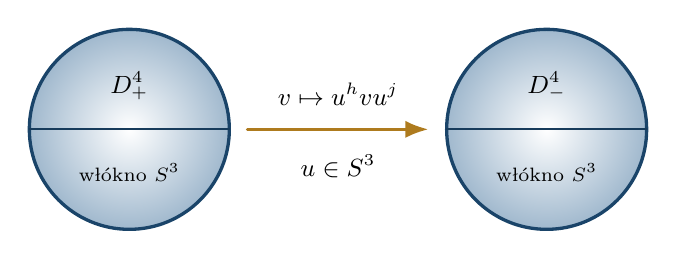
\begin{tikzpicture}[>=Latex,font=\small,line cap=round]
 \shade[inner color=white,outer color=manifoldblue!43]
      (-2.65,0) circle (1.27);
 \shade[inner color=white,outer color=manifoldblue!43]
      (2.65,0) circle (1.27);
 \draw[manifoldblue!75!black,very thick]
      (-2.65,0) circle (1.27)
      (2.65,0) circle (1.27);
 \draw[manifoldblue!65!black,thick]
      (-3.92,0)--(-1.38,0)
      (1.38,0)--(3.92,0);
 \node at (-2.65,.55) {$D^4_+$};
 \node at (2.65,.55) {$D^4_-$};
 \node[align=center,font=\scriptsize]
      at (-2.65,-.55) {włókno $S^3$};
 \node[align=center,font=\scriptsize]
      at (2.65,-.55) {włókno $S^3$};
 \draw[->,very thick,manifoldgold!85!black]
      (-1.15,0)--(1.15,0);
 \node[above,align=center] at (0,.18)
      {$v\mapsto u^hvu^j$};
 \node[below] at (0,-.20)
      {$u\in S^3$};
\end{tikzpicture}
\caption{Schemat sklejania wiązki nad dwiema
półsferami $S^4$. Kolorowe okręgi oznaczają
półsfery w umownym przekroju; zmienna $u$
parametryzuje ich wspólny równik. Odwzorowanie na strzałce
skręca włókno i określa gładką wiązkę.}
\label{fig:milnor-clutching-25}
\end{figure}

\begin{stwierdzenie}[Dwie liczby charakterystyczne]
\label{prop:milnor-classes-25}
Niech $\alpha$ będzie dodatnim generatorem
$H^4(S^4;\Z)\cong\Z$. Przy spójnie
ustalonych orientacjach
\[
 e(E_{h,j})=(h+j)\alpha,\qquad
 p_1(E_{h,j})=\pm2(h-j)\alpha.
\]
Znak w drugim wzorze zależy od przyjętej
identyfikacji dwóch czynników $\operatorname{Spin}(4)$
z parametrami $(h,j)$. Przy ustalonych konwencjach
jest określony; w późniejszym rachunku
występuje jego kwadrat.
\end{stwierdzenie}
\begin{proof}
Klasa Eulera wiązki orientowanej
nad $S^4$ mierzy stopień
odwzorowania $S^3\to S^3$
otrzymanego z funkcji sklejającej
przez zastosowanie jej do jednego
ustalonego wektora jednostkowego.
Istotnie, stałe przekroje jednostkowe
na obu półsferach przedłużają się osobno;
na równiku różnią się właśnie takim
odwzorowaniem do $S^3$, a jego stopień
jest przeszkodą do przedłużenia
przekroju bez zer przez drugą półsferę.
Dla $v=1$ w~\eqref{eq:milnor-clutching-25}
jest to $u\mapsto u^{h+j}$.
Mnożenie punktowe odwzorowań
$S^3\to S^3$ dodaje ich klasy
w $\pi_3(S^3)\cong\Z$, więc stopień
tego odwzorowania wynosi $h+j$.
To dowodzi wzoru na $e$.

Wyprowadzimy również współczynnik przy $p_1$
z dwóch prostych wiązek. Dla klasy
charakterystycznej $c$ czwartego stopnia
(tutaj $c=e$ lub $c=p_1$)
przepis
\[
 [g]\in\pi_3(SO(4))\longmapsto
 \langle c(E_g),[S^4]\rangle\in\Z
\]
jest homomorfizmem. Rzeczywiście dodawanie
klas sklejania można przedstawić przez
odwzorowanie ściskające równik na dwie sfery;
fundamentalna klasa $S^4$ przechodzi wtedy
na sumę ich klas fundamentalnych, a
naturalność $c$ dodaje oba parowania.
Ponieważ lewa i prawa multiplikacja
komutują, klasa~\eqref{eq:milnor-clutching-25}
jest sumą $h$ kopii klasy $(1,0)$
i $j$ kopii klasy $(0,1)$.

Wiązka $E_{1,0}$ jest kwaternioniczną
wiązką Hopfa. Mnożenie z lewej strony
jest liniowe względem ustalonej struktury
zespolonej danej mnożeniem z prawej przez $i$.
Otrzymujemy zespoloną wiązkę rangi $2$
o grupie strukturalnej $SU(2)$, więc $c_1=0$.
Jej $c_2$ jest, z dokładnością do znaku
orientacji, klasą Eulera wiązki rzeczywistej,
czyli generatorem $H^4(S^4;\Z)$:
obie klasy liczą zera poprzecznego przekroju,
przy czym $c_2$ używa orientacji zespolonej.
Tożsamość
$p_1(V_{\R})=c_1(V)^2-2c_2(V)$
daje $p_1(E_{1,0})=\pm2\alpha$.
Można ją sprawdzić po rozszczepieniu
$V$ na linie z formalnymi klasami
$x,y$: kompleksyfikacja $V_{\R}$
ma pierwiastki $x,y,-x,-y$, zatem
$-c_2(V_{\R}\otimes\C)=x^2+y^2
=(x+y)^2-2xy$. To jest właśnie
definicja $p_1$ z
Rozdziału~\ref{ch:przeciecia-dualnosc-klasy}.

Sprzężenie kwaternionowe $v\mapsto\bar v$
przenosi przejście $v\mapsto vu$ dla
$E_{0,1}$ na $\bar v\mapsto u^{-1}\bar v$.
Jako wiązki bez ustalonej orientacji
$E_{0,1}$ i $E_{-1,0}$ są więc izomorficzne.
Klasa $p_1$ nie zależy od orientacji włókna,
stąd $p_1(E_{0,1})=-p_1(E_{1,0})$.
Addytywność z poprzedniego akapitu kończy
rachunek: $p_1(E_{h,j})=\pm2(h-j)\alpha$,
z jednym spójnym wyborem znaku.
Zasada rozszczepiania użyta w rachunku
klas jest przywołana także w
Sekcji~\ref{sec:chern-weil-26};
ten sam wzór Milnor otrzymuje przez
addytywność $p_1$, zmianę orientacji
włókna i obliczenie dla wiązki Hopfa
w lemacie 3
\href{https://sites.math.rutgers.edu/~feehan/teaching/math866/milnor7sphere.pdf}
{Milnora, \emph{On Manifolds Homeomorphic to
the 7-Sphere} (1956)}.
\end{proof}

\section{Dlaczego całkowita przestrzeń jest
sferą homotopijną?}
\label{sec:milnor-homotopy-25}

Niech $h+j=1$. Zastosujmy
Mayera--Vietorisa do dwóch części
$M_{h,j}$ leżących nad półsferami.
Każda ma typ homotopijny $S^3$,
a ich część wspólna ma typ
$S^3_{\text{baza}}\times
S^3_{\text{włókno}}$.
Na grupach $H_3$ odwzorowanie z części
wspólnej do sumy homologii
obu połówek ma, po wyborze baz,
macierz
\begin{equation}\label{eq:milnor-MV-25}
 \begin{pmatrix}
 0&1\\
 h+j&1
 \end{pmatrix}.
\end{equation}
Pierwsza kolumna odpowiada
równikowi bazy. W pierwszej
trywializacji jest on brzegiem
dysku; w drugiej jego obraz
we włóknie ma stopień $h+j$.
Druga kolumna to sfera włókna,
generator $H_3$ w obu częściach.
Znaki jednego wiersza można
odwrócić zgodnie z konwencją
ciągu Mayera--Vietorisa;
wyznacznik ma wartość
bezwzględną $|h+j|$.
Przy $h+j=1$ macierz jest więc
automorfizmem $\Z^2$. Ponieważ
$H_4$ obu połówek i ich części
wspólnej jest zerowe, fragment
ciągu dokładnego ma postać
\[
 0\longrightarrow H_4(M_{h,j})
 \longrightarrow\Z^2
 \xrightarrow{\ A\ }
 \Z^2\longrightarrow H_3(M_{h,j})
 \longrightarrow0.
\]
Tutaj $A$ jest macierzą z~\eqref{eq:milnor-MV-25}.
Jądro $A$ i iloraz $\Z^2/\operatorname{im}A$
są zerowe,
więc $H_4(M_{h,j})=H_3(M_{h,j})=0$.
Widać też, dlaczego warunek na klasę
Eulera jest rozstrzygający: dla
$h+j=m\ne0$ ten sam fragment daje
$H_3(M_{h,j})\cong\Z/|m|\Z$,
a więc tylko $|m|=1$ może dać
sferę homologijną.
Pozostałe wyrazy tego samego
ciągu dają
\[
 H_i(M_{h,j};\Z)=
 \begin{cases}
 \Z,&i=0,7,\\
 0,&0<i<7.
 \end{cases}
\]
Rzeczywiście odwzorowanie łączące
$H_7(M_{h,j})\to H_6(S^3\times S^3)$
jest izomorfizmem, a w innych
stopniach dodatnich poza trzecim
grupy części są zerowe.

Długi ciąg homotopii rozwłóknienia
$S^3\to M_{h,j}\to S^4$ daje
$\pi_1(M_{h,j})=0$.
Wybierzmy zanurzony zamknięty dysk
$D^7\subset M_{h,j}$. Zwińmy do punktu
zamknięty zbiór
$M_{h,j}\setminus\operatorname{int}D^7$.
Iloraz jest homeomorficzny z $S^7$,
otrzymujemy więc, po zgodnym wyborze
orientacji, odwzorowanie stopnia jeden
$M_{h,j}\to S^7$.
Obliczone grupy homologii pokazują,
że jest ono izomorfizmem homologii.
Obie rozmaitości mają typ kompleksów CW,
więc homologiczne kryterium Whiteheada
(Wniosek~\ref{cor:whitehead-homologiczny})
daje równoważność homotopijną.
Zatem $M_{h,j}$ jest gładką
sferą homotopijną, a przez
Twierdzenie~\ref{thm:poincare-high-24}
jest homeomorficzna z $S^7$.

\section{Niezmiennik wykrywający egzotyczność}
\label{sec:milnor-invariant-25}

Sama homologia i równoważność
homotopijna nie rozstrzygają
o dyfeomorfizmie. Potrzebujemy
niezmiennika gładkiego.
Załóżmy, że $M^7$ jest
zorientowaną rozmaitością
z $H^3(M;\Z)=H^4(M;\Z)=0$
i że $M=\partial B$ dla
zorientowanej gładkiej
$8$-rozmaitości $B$.
W długim ciągu pary
odwzorowanie
$j:H^4(B,M;\Z)\to H^4(B;\Z)$
jest izomorfizmem.
Dlatego $p_1(TB)$ ma
jednoznaczne względne podniesienie
$\bar p_1=j^{-1}p_1(TB)$.
Połóżmy
\[
 q(B)=\langle
    \bar p_1\smile p_1(TB),[B,M]\rangle,
 \qquad
 \lambda(M)=[\,2q(B)-\operatorname{sign}(B)\,]
                    \in\Z/7.
\]
Sygnatura $\operatorname{sign}(B)$
jest sygnaturą formy przecięcia
na obrazie
$H_4(B;\Q)\to H_4(B,M;\Q)$;
przejście do $\Q$ usuwa torsję,
na której sygnatura nie jest określona.
Na przykład dla $M=S^7$
można wziąć $B=D^8$,
co daje $q(B)=0$ i
$\lambda(S^7)=0$.

\begin{twierdzenie}[Milnor: niezależność
od wypełnienia]
\label{thm:milnor-invariant-25}
Powyższa klasa $\lambda(M)\in\Z/7$
nie zależy od wybranego gładkiego
zorientowanego wypełnienia $B$.
Jest więc niezmiennikiem
zorientowanego dyfeomorfizmu $M$.
\end{twierdzenie}
\begin{proof}
Niech $B_0,B_1$ będą dwoma
wypełnieniami. Sklejmy
$C=B_0\cup_M(-B_1)$;
to zamknięta zorientowana
$8$-rozmaitość. Z przyjętych założeń
mamy $H^3(M)=H^4(M)=0$.
Długie ciągi par $(B_i,M)$ dają
izomorfizmy
$H^4(B_i,M)\xrightarrow{\sim}H^4(B_i)$.
W ciągu Mayera--Vietorisa dla $C$
znikają $H^3(M)$ i $H^4(M)$,
więc klasy czwarte obu części
sklejają się jednoznacznie:
$H^4(C)\cong H^4(B_0)\oplus H^4(B_1)$.
Izomorfizmy $j$ pozwalają wybrać
ich reprezentanty względne, zerowe
na małych kołnierzach wspólnego brzegu.
Po przedłużeniu przez zero na drugi
kawałek iloczyn dwóch klas z różnych
kawałków ma zerowe parowanie z $[C]$.
Naturalność klas Pontriagina i rozkład
orientacji na dwóch sklejonych
kawałkach dają więc
sumę parowań z obu części, z minusem
przy drugim wypełnieniu. Ponadto
dualność Poincarégo na $M$ daje
$H_4(M;\Q)=H_3(M;\Q)=0$.
Ciągi par $(B_i,M)$ utożsamiają więc
$H_4(B_i;\Q)$ z $H_4(B_i,M;\Q)$,
a ciąg Mayera--Vietorisa rozkłada
$H_4(C;\Q)$ na sumę grup obu kawałków.
Ich klasy mają rozłączne reprezentanty,
więc forma przecięcia na $C$ jest
sumą ortogonalną form tych kawałków.
Dlatego
\[
 q(C)=q(B_0)-q(B_1),\qquad
 \operatorname{sign}(C)
  =\operatorname{sign}(B_0)
   -\operatorname{sign}(B_1).
\]
Na zamkniętej $C$ mamy
$q(C)=\langle p_1(C)^2,[C]\rangle$.
Zastosujmy wzór Hirzebrucha
na sygnaturę w wymiarze osiem:
\[
 45\operatorname{sign}(C)=
 \langle 7p_2(C)-p_1(C)^2,[C]\rangle.
\]
Współczynniki $7,-1,45$ można sprawdzić
formalnie bez dowodzenia samego twierdzenia
Hirzebrucha. Dla formalnych pierwiastków
Pontriagina $x_a$ rozwijamy
$x/\tanh x=1+x^2/3-x^4/45+\cdots$.
Składnik stopnia osiem iloczynu wynosi
\[
 \frac1{9}\sum_{a<b}x_a^2x_b^2
 -\frac1{45}\sum_a x_a^4
 =\frac{7p_2-p_1^2}{45},
 \quad p_1=\sum_a x_a^2,\quad
 p_2=\sum_{a<b}x_a^2x_b^2.
\]
Głębokim wejściem jest identyfikacja
parowania tego wielomianu z sygnaturą
każdej \emph{zamkniętej} zorientowanej
$8$-rozmaitości; nie stosujemy jej
bezpośrednio do $B$ z brzegiem. W tej
postaci używa jej
\href{https://sites.math.rutgers.edu/~feehan/teaching/math866/milnor7sphere.pdf}
{Milnor, \emph{On Manifolds Homeomorphic
to the 7-Sphere}, §1}.
Stąd
\[
 45\bigl(2q(C)-\operatorname{sign}(C)\bigr)
 =
 \langle 91p_1(C)^2-7p_2(C),[C]\rangle.
\]
Prawa strona dzieli się przez $7$.
Ponieważ $45$ jest odwracalne
modulo $7$, również
$2q(C)-\operatorname{sign}(C)$
jest podzielne przez $7$.
Po podstawieniu wzorów
addytywności otrzymujemy
$\lambda_{B_0}(M)=\lambda_{B_1}(M)$.
Użyty wzór Hirzebrucha jest
głębokim wynikiem zewnętrznym;
to właśnie on jest istotną
częścią argumentu Milnora.
\end{proof}

\begin{stwierdzenie}[Rachunek dla wiązek Milnora]
\label{prop:milnor-value-25}
Dla nieparzystego $k$ wybierzmy
\[
 h=\frac{k+1}{2},\qquad
 j=\frac{1-k}{2},
 \qquad M_k=M_{h,j}.
\]
Wtedy
\[
 \lambda(M_k)
 =8k^2-1\equiv k^2-1\pmod7.
\]
\end{stwierdzenie}
\begin{proof}
Mamy $h+j=1$, więc
poprzednia sekcja pokazuje,
że $M_k$ jest sferą homotopijną.
Wiązka dysków $B_k=D(E_{h,j})$
deformuje się na zerowy przekrój
$S^4$, dlatego
$H^4(B_k;\Z)=\Z\alpha$.
Po wybraniu połączenia na $E_{h,j}$
ciąg styczny
$0\to\pi^*E_{h,j}\to TB_k
\to\pi^*TS^4\to0$
rozszczepia się, więc
$TB_k\cong\pi^*TS^4\oplus\pi^*E_{h,j}$.
Ze Stwierdzenia~\ref{prop:milnor-classes-25}
otrzymujemy
$p_1(TB_k)=\pm2k\alpha$:
wiązka $TS^4$ jest stabilnie
trywialna, zatem jej $p_1=0$.
Forma przecięcia w środku
$B_k$ ma macierz $[1]$,
ponieważ samoprzecięcie
zerowego przekroju jest liczbą
Eulera $e(E_{h,j})=1$.
Stąd $\operatorname{sign}(B_k)=1$.
Twierdzenie Thoma
(Twierdzenie~\ref{thm:euler-thom-16})
daje generator $U\in H^4(B_k,M_k;\Z)$
oraz tożsamość $j(U)=\pi^*e(E_{h,j})$.
Stąd $U\smile j(U)=
\pi^*e(E_{h,j})\smile U$, a parowanie
tej klasy z $[B_k,M_k]$ jest równe
$\langle e(E_{h,j}),[S^4]\rangle=1$.
Otrzymujemy
$q(B_k)=(2k)^2=4k^2$,
a po podstawieniu do definicji
$\lambda$ dostajemy
$2\cdot4k^2-1$.
\end{proof}

\begin{twierdzenie}[Egzotyczna sfera Milnora]
\label{thm:exotic-milnor-25}
Rozmaitość $M_3^7$ otrzymana
dla $(h,j)=(2,-1)$
jest homeomorficzna z $S^7$,
ale nie jest z nią dyfeomorficzna.
\end{twierdzenie}
\begin{proof}
Warunek $h+j=1$ i obliczenie
homologii pokazują, że
$M_3\simeq S^7$; homeomorfizm
wynika z
Twierdzenia~\ref{thm:poincare-high-24}.
Natomiast
$\lambda(M_3)=8\cdot9-1=71
\equiv1\pmod7$, podczas gdy
$\lambda(S^7)=0$.
Gdyby istniał dyfeomorfizm
zachowujący orientację, te
niezmienniki musiałyby być równe.
Odwrócenie orientacji zmienia
znak $\lambda$: wypełnienie $-B$
ma przeciwną klasę fundamentalną,
więc $q(-B)=-q(B)$ oraz
$\operatorname{sign}(-B)
=-\operatorname{sign}(B)$.
Liczba $\pm1$
nadal nie jest zerem modulo $7$.
Zatem nie istnieje także
dyfeomorfizm odwracający
orientację.
\end{proof}

\subsection*{Dokładniejsze rozróżnienie: Eells--Kuiper}

Niezmiennik Milnora ma wartości w $\Z/7$,
więc może utożsamiać sfery, które różnią
się gładko. Dla sfer homologijnych wymiaru
siedem struktura spin pozwala wykorzystać
silniejszą podzielność liczb
charakterystycznych zamkniętych
$8$-rozmaitości. Jest to intuicja
niezmiennika Eellsa--Kuipera.

Niech $M^7$ będzie zorientowaną sferą
homologiczną i niech $B^8$ będzie zwartym,
zorientowanym \emph{spinowym} wypełnieniem
$M$. Struktura spin na $M$ jest jedyna,
bo $H^1(M;\Z/2)=0$. Jak poprzednio
$p_1(TB)$ ma jednoznaczne względne
podniesienie $\bar p_1$; używając
tego samego $q(B)$, definiujemy
\[
 \mu(M)=
 \left[\frac{q(B)-4\operatorname{sign}(B)}
                 {2^7\cdot7}\right]\in\Q/\Z.
\]
Warunek istnienia spinowego wypełnienia
jest częścią tej definicji. W szczególności
spełniają go wszystkie skonstruowane tu
$M_k$, ponieważ $B_k=D(E_{h,j})$ jest
spinowa: $TB_k\cong
\pi^*(TS^4\oplus E_{h,j})$ i
$H^2(S^4;\Z/2)=0$.

\begin{stwierdzenie}[Niezależność $\mu$ od
 spinowego wypełnienia]
\label{prop:eells-kuiper-Milnor-25}
W powyższych hipotezach $\mu(M)$ zależy
tylko od zorientowanej klasy
dyfeomorfizmu $M$; ponadto
$\mu(-M)=-\mu(M)$.
Dla sfer Milnora o nieparzystym $k$ mamy
\[
 \mu(M_k)=\frac{k^2-1}{224}\pmod{\Z}.
\]
\end{stwierdzenie}
\begin{proof}
Dla dwóch wypełnień spinowych sklejamy
$C=B_0\cup_M(-B_1)$. Jedyna struktura
spin na $M$ zapewnia zgodność struktur
na kołnierzu, więc $C$ jest zamkniętą
spinową $8$-rozmaitością.
Rachunek względnych klas z dowodu
Twierdzenia~\ref{thm:milnor-invariant-25}
daje
\[
 q(C)=q(B_0)-q(B_1),\qquad
 \operatorname{sign}(C)=
 \operatorname{sign}(B_0)
 -\operatorname{sign}(B_1).
\]
Dla zamkniętej zorientowanej
$8$-rozmaitości twierdzenie Hirzebrucha
daje
\[
 45\operatorname{sign}(C)
   =7\langle p_2(C),[C]\rangle
      -\langle p_1(C)^2,[C]\rangle.
\]
Ponadto twierdzenie o indeksie operatora
Diraca mówi, że dla \emph{zamkniętej
spinowej} $C$ liczba
\[
 \widehat A(C)=
 \frac{7\langle p_1(C)^2,[C]\rangle
       -4\langle p_2(C),[C]\rangle}
      {5760}
\]
jest całkowita. Eliminując $p_2(C)$
z tych dwóch wzorów, otrzymujemy
\[
 q(C)-4\operatorname{sign}(C)
   =896\,\widehat A(C)\in896\Z.
\]
Stąd dwie wartości w definicji $\mu$
różnią się o liczbę całkowitą.
Odwrócenie orientacji zmienia znaki
$q$ i sygnatury, więc zmienia też
znak $\mu$.

Dla $B_k$ obliczyliśmy
$q(B_k)=4k^2$ i
$\operatorname{sign}(B_k)=1$.
Podstawienie daje
$(4k^2-4)/896=(k^2-1)/224$.
\end{proof}

Całkowitość indeksu Diraca jest tutaj
głębokim wynikiem zewnętrznym; wzór
i jego zastosowanie do tych wiązek
pochodzą z
\href{https://webhomes.maths.ed.ac.uk/~v1ranick/papers/eelskuip.pdf}
{J. Eellsa i N. Kuipera,
\emph{An Invariant for Certain Smooth
Manifolds}, §6}. Dla przykładu:
\[
\begin{array}{c|cccc}
 k&1&3&5&7\\ \hline
 \lambda(M_k)\in\Z/7&0&1&3&6\\
 \mu(M_k)\in\Q/\Z&0&1/28&3/28&6/28
\end{array}
\]
Wartość $\mu(S^7)=0$ z wypełnienia
$D^8$ potwierdza egzotyczność $M_3$.
Ponadto $1/28$, $3/28$ i $6/28$
nie są sobie równe nawet po zmianie
znaku w $\Q/\Z$, więc $M_3,M_5,M_7$
są parami niedyfeomorficzne również
bez wyboru orientacji.

W języku
Definicji~\ref{def:structure-set-23}
przykład daje strukturę na
typie homotopijnym $S^7$
różną od standardowej.

\section{Klasyfikacja gładkich sfer
 wymiaru siedem}

Niech $\Theta_7$ oznacza zbiór klas
zorientowanego dyfeomorfizmu
gładkich sfer homotopijnych wymiaru
siedem. Suma spójna $\#$ nadaje mu
strukturę grupy, której zerem jest
standardowa $S^7$, a odwrotnością
klasy $[M]$ jest $[-M]$.
W oryginalnym ujęciu $\Theta_7$ składa
się z klas $h$-kobordyzmu; w tym
wymiarze są one klasami dyfeomorfizmu
na mocy Twierdzenia~\ref{thm:smale-hc-19}.

Użyjemy dwóch głębokich wyników
\emph{jako twierdzeń zewnętrznych}.
\href{https://www.sas.rochester.edu/mth/sites/doug-ravenel/otherpapers/kervaire-milnor.pdf}
{Kervaire i Milnor, \emph{Groups of Homotopy
Spheres I}, \S\,4 oraz \S\S\,7--8}, wykazali
w wymiarze siedem, że
$\Theta_7=bP_8\cong\Z/28$; tutaj
$bP_8$ oznacza klasy sfer homotopijnych,
które ograniczają równoległawialne
$8$-rozmaitości. Zatem każda taka
sfera ma w szczególności wypełnienie
spinowe i jej $\mu$ jest określone.
\href{https://webhomes.maths.ed.ac.uk/~v1ranick/papers/eelskuip.pdf}
{Eells i Kuiper, \emph{An Invariant for
Certain Smooth Manifolds}, \S6,
s. 102--103}, dowiedli, że $\mu$ jest
\emph{zupełnym} niezmiennikiem
zorientowanego dyfeomorfizmu
gładkich sfer homeomorficznych z $S^7$.
Poprzednie stwierdzenie wykazało
jedynie niezależność $\mu$ od
wypełnienia oraz obliczyło jego
wartość dla $M_k$; nie zastępuje
cytowanego twierdzenia o zupełności.

\begin{twierdzenie}[Klasyfikacja sfer Milnora]
\label{thm:milnor-classification-25}
Niech $k,l$ będą nieparzyste, a
$M_k,M_l$ niech mają orientacje
brzegowe wypełnień $B_k,B_l$
o sygnaturze $+1$. Wtedy
\[
 M_k\cong M_l\quad\text{z zachowaniem orientacji}
 \quad\Longleftrightarrow\quad
 k^2\equiv l^2\pmod{224}.
\]
Rodzina $\{M_k:k\in2\Z+1\}$
reprezentuje dokładnie $16$ spośród
$28$ klas w $\Theta_7$.
\end{twierdzenie}
\begin{proof}
Zupełność $\mu$ z twierdzenia
Eellsa--Kuipera mówi, że dwa
zorientowane $M_k,M_l$ są
dyfeomorficzne wtedy i tylko wtedy,
gdy ich wartości $\mu$ są równe.
Ze Stwierdzenia~\ref{prop:eells-kuiper-Milnor-25}
wynika, że warunek ten ma postać
\[
 \frac{k^2-1}{224}-\frac{l^2-1}{224}
 \in\Z,
\]
co jest równoważne podanej kongruencji.

Policzmy liczbę możliwych wartości.
Zapiszmy $k=2h-1$, $h\in\Z$. Wówczas
\[
 \mu(M_{2h-1})
 =\frac{h(h-1)}{56}
 =\frac{1}{28}\,\frac{h(h-1)}2
 \pmod{\Z}.
\]
Wystarczy więc policzyć wartości
liczby trójkątnej
$t_h=h(h-1)/2$ modulo $28=4\cdot7$.
Dla $h$ modulo $8$ kolejne wartości
$t_h$ modulo $4$ to
$0,0,1,3,2,2,3,1$; występują
wszystkie cztery reszty. Dla $h$
modulo $7$ wartości $t_h$ modulo
$7$ to $0,0,1,3,6,3,1$;
występują dokładnie cztery reszty
$\{0,1,3,6\}$.
Reszty $h$ modulo $8$ i modulo $7$
można wybierać niezależnie na mocy
chińskiego twierdzenia o resztach.
Każda z $4\cdot4=16$ par reszt
określa inną wartość $t_h$ modulo
$28$, a każda jest osiągana.
Jawnie otrzymujemy
\[
 t_h\pmod{28}\ \in
 \{0,1,3,6,7,8,10,13,14,15,17,
   20,21,22,24,27\}.
\]
Podzielenie przez $28$ daje dokładnie
$16$ wartości $\mu(M_k)$ w $\Q/\Z$.
Zupełność $\mu$ kończy dowód liczby
klas dyfeomorfizmu.
\end{proof}

Pozostałe $12$ klas w $\Theta_7$
nie występuje wśród zorientowanych
$M_k$ z przyjętą tu orientacją
brzegową. Wszystkie klasy można
jednak otrzymać z jednej sfery
Milnora przez sumy spójne.

\begin{twierdzenie}[Wszystkie struktury gładkie na $S^7$]
\label{thm:all-seven-spheres-25}
Sfery
\[
 \underbrace{M_3\#\cdots\#M_3}_{r\ \text{składników}},
 \qquad r=0,1,\ldots,27,
\]
gdzie $r=0$ oznacza $S^7$,
reprezentują wszystkie $28$ klas
zorientowanego dyfeomorfizmu
gładkich sfer homotopijnych
wymiaru siedem, każdą dokładnie raz.
Po zapomnieniu orientacji pozostaje
$15$ klas dyfeomorfizmu, w tym
jedna klasa standardowa.
\end{twierdzenie}
\begin{proof}
Niezmiennik $\mu$ jest addytywny
względem sumy spójnej. Istotnie,
jeśli $B$ i $B'$ są spinowymi
wypełnieniami dwóch sfer
homotopijnych, to ich brzegowa
suma spójna jest spinowym
wypełnieniem $\partial B\#\partial B'$.
Dołożony uchwyt indeksu jeden nie
wnosi środkowej homologii; formy
przecięcia obu kawałków tworzą
sumę ortogonalną, a względne klasy
$p_1$ z obu kawałków nie mają
mieszanych iloczynów. Stąd $q$ i
sygnatura dodają się, więc również
$\mu(\partial B\#\partial B')
=\mu(\partial B)+\mu(\partial B')$.
Ponieważ $\mu(M_3)=1/28$, suma
$r$ kopii ma niezmiennik $r/28$
modulo $\Z$. Dla $r=0,\ldots,27$
są to różne wartości, zatem
otrzymujemy $28$ różnych klas
zorientowanego dyfeomorfizmu.
Twierdzenie Kervaire'a--Milnora
stwierdza, że innych klas nie ma.

Odwrócenie orientacji zmienia
$\mu$ na $-\mu$. Ponieważ $\mu$
klasyfikuje sfery zorientowane,
zapomnienie orientacji utożsamia
reszty $r$ i $-r$ modulo $28$.
Samymi swoimi przeciwieństwami
są tylko $r=0$ i $r=14$, bo
$2r\equiv0\pmod{28}$ właśnie
dla tych dwóch reszt. Pozostałe
$26$ reszt tworzy $13$ par.
Łącznie daje to $2+13=15$
klas bez wybranej orientacji.
\end{proof}

\par\smallskip
{\footnotesize\noindent\emph{Dalsza lektura:}
\href{https://sites.math.rutgers.edu/~feehan/teaching/math866/milnor7sphere.pdf}
{J.\ Milnor, \emph{On Manifolds Homeomorphic
to the 7-Sphere}, Ann. of Math. 64 (1956),
§1--3}. W oryginale homeomorfizm
uzyskano przez specjalną funkcję
Morse'a; tutaj użyliśmy
Twierdzenia~\ref{thm:poincare-high-24}.\par}

\clearpage


\part{Potok Ricciego i topologia wymiaru trzy}
\chapter{Potok Ricciego: metryka, krzywizna i pierwsze równania ewolucyjne}
\label{ch:potok-ricciego}
\index{potok Ricciego}

Metryka pozwala mierzyć długości i objętości, a tensor Ricciego
opisuje część jej krzywizny. Można więc zapytać, co się stanie,
gdy metrykę będziemy zmieniać z prędkością wyznaczoną przez
ten tensor. Na sferze oczekujemy kurczenia, ponieważ jej Ricci
jest dodatni; płaski torus powinien pozostać nieruchomy.
Oba przewidywania sprawdzimy rachunkiem. Następnie wyprowadzimy
równania dla miary i krzywizny skalarnej oraz wyjaśnimy, gdzie
w dowodzie istnienia rozwiązania potrzebna jest analiza równań
parabolicznych.

W całym rozdziale $M^n$ jest gładką, zwartą rozmaitością bez
brzegu, $n\geq2$, a metryki są riemannowskie. Orientacja nie jest
potrzebna do określenia gęstości objętości. Zachowujemy konwencję
krzywizny z Definicji~\ref{def:tensor-krzywizny}: okrągła sfera
ma dodatni tensor Ricciego. Piszemy
\[
 \Delta_g f=\operatorname{div}_g(\nabla^g f)
            =g^{ij}\nabla_i\nabla_j f.
\]
Jest to konwencja z rozdziału~\ref{ch:krzywizna}; na zwartej
rozmaitości $\int_M f\Delta_g f\,\dd\mu_g
=-\int_M|\nabla f|_g^2\,\dd\mu_g$. Na orientowalnej $M$
laplasjan Hodge'a z Rozdziału~\ref{ch:hodge-bochner},
$\Delta_H=\dd\delta+\delta\dd$, spełnia na funkcjach
$\Delta_H=-\Delta_g$. To rozróżnienie ustala
znak wszystkich poniższych równań cieplnych.

\section{Równanie i metryki o stałej krzywiźnie}
\label{sec:ricci-flow-definition}

\begin{definicja}[Potok Ricciego Hamiltona]
\label{def:ricci-flow}
Niech $g_0$ będzie gładką metryką na $M$. \emph{Potokiem
Ricciego} o wartości początkowej $g_0$ na przedziale $[0,T)$
nazywamy gładką rodzinę metryk $g(t)$ spełniającą
\begin{equation}\label{eq:ricci-flow}
 \partial_tg(t)=-2\operatorname{Ric}(g(t)),
 \qquad g(0)=g_0.
\end{equation}
Jest to wersja \emph{nienormalizowana}: nie dodajemy składnika,
który utrzymywałby całkowitą objętość na stałym poziomie.
\end{definicja}


\begin{figure}[htbp]
\centering
\begin{tikzpicture}[>=Stealth, font=\small]

% Podpisy etapów
\node[align=center] at (2.20,6.55)
  {\textbf{Metryka początkowa}\\[2pt]$(\mathbb R^3,g(t_0))$};

\node[align=center] at (7.35,6.55)
  {\textbf{Etap pośredni}\\[2pt]$(\mathbb R^3,g(t_1))$};

\node[align=center] at (12.50,6.55)
  {\textbf{Geometria bardziej jednorodna}\\[2pt]$(\mathbb R^3,g(t_2))$};

% Trzy schematyczne powierzchnie siatkowe
% A: wielkość wybrzuszenia
% B: głębokość zwężeń
\foreach \X/\A/\B in {
  0/0.72/0.36,
  5.15/0.34/0.16,
  10.30/0.00/0.00
}{
  \begin{axis}[
    at={(\X cm,1.12cm)},
    anchor=south west,
    width=4.40cm,
    height=4.85cm,
    scale only axis,
    hide axis,
    view={50}{18},
    xmin=-2.05,xmax=2.05,
    ymin=-2.05,ymax=2.05,
    zmin=-1.8,zmax=1.8,
    z buffer=sort,
    samples=34,
    samples y=17,
    domain=0:360,
    y domain=-1.7:1.7,
    colormap={mojniebieski}{
      rgb255=(213,239,253)
      rgb255=(154,205,239)
    }
  ]

  \addplot3[
    surf,
    shader=faceted,
    faceted color=blue!50!black,
    line width=0.16pt,
    opacity=0.78
  ]
  (
    {
      (1+\A*exp(-3*y*y)
      -\B*(exp(-6*(y-1.03)^2)
      +exp(-6*(y+1.03)^2)))*cos(x)
    },
    {
      (1+\A*exp(-3*y*y)
      -\B*(exp(-6*(y-1.03)^2)
      +exp(-6*(y+1.03)^2)))*sin(x)
    },
    {y}
  );

  \end{axis}
}

% Strzałki ewolucji
\draw[->,very thick]
  (4.52,3.47)--(5.02,3.47);

\draw[->,very thick]
  (9.67,3.47)--(10.17,3.47);

% Oś czasu i równanie potoku
\draw[->,thick]
  (0.25,-0.10)--(14.75,-0.10);

\node[fill=white,inner sep=2pt]
  at (7.50,-0.10)
  {
    $\displaystyle
    \partial_t g
    =-2\operatorname{Ric}(g),
    \qquad t_0<t_1<t_2
    $
  };

\end{tikzpicture}

\caption{Schemat ideowy zmiany geometrii na
$\mathbb R^3$ w potoku Ricciego
$\partial_t g=-2\operatorname{Ric}(g)$.
Niebieskie powierzchnie siatkowe symbolizują
zmniejszanie się wybranej lokalnej deformacji;
nie są reprezentacją całej trójwymiarowej metryki.
Rysunek nie zakłada, że dowolny potok Ricciego
zbiega do metryki euklidesowej.}
\label{fig:ricci-r3-schemat}
\end{figure}


Dla wektora $v\in T_pM$, trzymanego nieruchomo przy zmianie
czasu, równanie daje
\[
 \frac{\dd}{\dd t}|v|_{g(t)}^2
 =-2\operatorname{Ric}_{g(t)}(v,v).
\]
Dodatni Ricci zmniejsza więc kwadrat długości w danym
kierunku; ujemny go zwiększa. Nazwa „potok” oznacza tu
ewolucję tensora metrycznego, a nie przepływ punktów
rozmaitości z rozdziału~\ref{ch:pola}.

\begin{stwierdzenie}[Stała zmiana skali]
\label{prop:ricci-scaling}
Jeżeli $g_0$ jest metryką i $c>0$ jest liczbą niezależną
od punktu $M$, to dla $\widetilde g=cg_0$ zachodzi
\[
 \nabla^{\widetilde g}=\nabla^{g_0},\qquad
 \operatorname{Ric}(\widetilde g)=\operatorname{Ric}(g_0),
 \qquad \operatorname{Scal}(\widetilde g)
          =c^{-1}\operatorname{Scal}(g_0),
\]
\[
 K_{\widetilde g}=c^{-1}K_{g_0},\qquad
 \dd\mu_{\widetilde g}=c^{n/2}\dd\mu_{g_0}.
\]
Wzór na $K$ dotyczy każdej płaszczyzny stycznej.
\end{stwierdzenie}
\begin{proof}
W mapie $\widetilde g_{ij}=cg_{0,ij}$ i
$\widetilde g^{ij}=c^{-1}g_0^{ij}$. We wzorze na symbole
Christoffela~\eqref{eq:christoffel-metryka} czynnik $c$
z pochodnych metryki znosi $c^{-1}$ z macierzy
odwrotnej. Koneksja i operator $R(X,Y)Z$ są więc
niezmienione. Ricci z rozdziału~\ref{ch:krzywizna}
jest śladem endomorfizmu $W\mapsto R(W,X)Y$, zatem
również się nie zmienia jako tensor typu $(0,2)$.
Skalar wymaga jeszcze kontrakcji z
$\widetilde g^{ij}=c^{-1}g_0^{ij}$.

W ilorazie definiującym krzywiznę sekcyjną
\eqref{eq:krzywizna-sekcyjna} licznik jest liniowy
w metryce i mnoży się przez $c$, a wyznacznik
macierzy Grama w mianowniku przez $c^2$. Wreszcie
$\det(cg_{0,ij})=c^n\det(g_{0,ij})$; pierwiastek
wyznacznika daje ostatnią równość.
\end{proof}

\begin{stwierdzenie}[Metryka Einsteina jako rozwiązanie]
\label{prop:ricci-einstein-flow}
Załóżmy, że $\operatorname{Ric}(g_0)=\lambda g_0$
z pewną stałą $\lambda\in\R$. Wtedy
\begin{equation}\label{eq:ricci-einstein-solution}
 g(t)=(1-2\lambda t)g_0
\end{equation}
spełnia~\eqref{eq:ricci-flow} na każdym przedziale,
na którym $1-2\lambda t>0$. Gdy $\lambda>0$,
rozwiązanie tego kształtu kończy się przy
$t=(2\lambda)^{-1}$; gdy $\lambda=0$, jest stacjonarne;
gdy $\lambda<0$, skala rośnie.
\end{stwierdzenie}
\begin{proof}
Wstawmy $g(t)=c(t)g_0$ z $c(0)=1$. Ponieważ
$c(t)$ jest stałe na $M$, Stwierdzenie~\ref{prop:ricci-scaling}
daje $\operatorname{Ric}(g(t))=\lambda g_0$.
Równanie~\eqref{eq:ricci-flow} przyjmuje postać
$c'(t)g_0=-2\lambda g_0$, czyli $c'=-2\lambda$.
Całkując z warunkiem $c(0)=1$, dostajemy podany wzór.
Dodatniość $c(t)$ jest konieczna, by tensor był metryką.
\end{proof}

\begin{przyklad}[Okrągła sfera]
\label{prz:ricci-sphere}
Niech $g_{\mathrm{jedn}}$ będzie metryką sfery jednostkowej
$S^n$, a $g_0=a_0^2g_{\mathrm{jedn}}$, $a_0>0$.
Z~\eqref{eq:stala-krzywizna-tensor} i
Stwierdzenia~\ref{prop:ricci-scaling} otrzymujemy
\[
 \operatorname{Ric}(g_0)
 =(n-1)g_{\mathrm{jedn}}
 =\frac{n-1}{a_0^2}g_0.
\]
Zatem rozwiązanie z poprzedniego stwierdzenia ma postać
\begin{equation}\label{eq:ricci-sphere}
 g(t)=a(t)^2g_{\mathrm{jedn}},\qquad
 a(t)^2=a_0^2-2(n-1)t,
 \qquad 0\leq t<\frac{a_0^2}{2(n-1)}.
\end{equation}
Promień $a(t)$ maleje, a $K(t)=a(t)^{-2}$ rośnie.
W chwili granicznej tensor traci dodatnią określoność;
nie jest to gładkie przedłużenie potoku przez tę chwilę.
Dla $n=2$ pole powierzchni wynosi
$4\pi a(t)^2=4\pi a_0^2-8\pi t$.
\end{przyklad}

\begin{przyklad}[Płaski torus]
\label{prz:ricci-torus}
Niech $T^n=\R^n/\Lambda$ dla kraty $\Lambda$,
a $g_0$ niech będzie metryką pochodzącą od stałego
dodatnio określonego iloczynu skalarnego na $\R^n$.
W tych współrzędnych symbole Christoffela i tensor
krzywizny są zerowe, więc $\operatorname{Ric}(g_0)=0$.
Rodzina $g(t)=g_0$ spełnia~\eqref{eq:ricci-flow}.
W szczególności płaski torus dwuwymiarowy zachowuje
swój kształt i pole. Sam warunek $\chi(T^2)=0$ nie mówi,
że \emph{każda} metryka torusa jest płaska; dla innych
metryk pole pozostanie stałe, choć metryka może się
zmieniać.
\end{przyklad}

\section{Ewolucja miary i krzywizny skalarnej}
\label{sec:ricci-evolution}

\begin{stwierdzenie}[Zmiana elementu objętości]
\label{prop:ricci-volume}
Dla dowolnej gładkiej rodziny metryk o
$h=\partial_tg$ mamy
\[
 \partial_t\dd\mu_g
   =\tfrac12\operatorname{tr}_g h\,\dd\mu_g.
\]
Wzdłuż potoku Ricciego wynika stąd
\begin{equation}\label{eq:ricci-volume}
 \partial_t\dd\mu_g=-\operatorname{Scal}_g\,\dd\mu_g,
 \qquad
 \frac{\dd}{\dd t}\operatorname{Vol}_{g(t)}(M)
 =-\int_M\operatorname{Scal}_{g(t)}\,\dd\mu_{g(t)}.
\end{equation}
\end{stwierdzenie}
\begin{proof}
W mapie gęstość objętości to
$\sqrt{\det(g_{ij})}\,|\dd x^1\cdots\dd x^n|$.
Wzór Jacobiego na pochodną wyznacznika daje
\[
 \partial_t\det(g_{ij})
 =\det(g_{ij})\operatorname{tr}(g^{-1}h)
 =\det(g_{ij})g^{ij}h_{ij}.
\]
Pochodna pierwiastka wprowadza czynnik $1/2$.
Dla $h=-2\operatorname{Ric}$ ślad wynosi
$-2\operatorname{Scal}$. Zwarta rozmaitość pozwala
różniczkować całkę po $M$ pod znakiem całkowania.
\end{proof}

Do równania dla skalara potrzebujemy jednej tożsamości
wynikającej z krzywizny koneksji Leviego-Civity.

\begin{lemat}[Ściągnięta druga tożsamość Bianchiego]
\label{lem:ricci-contracted-bianchi}
Dla każdej gładkiej metryki riemannowskiej
\begin{equation}\label{eq:ricci-contracted-bianchi}
 \nabla^i\operatorname{Ric}_{ij}
       =\tfrac12\nabla_j\operatorname{Scal}.
\end{equation}
\end{lemat}
\begin{proof}
Użyjmy oznaczeń z~\eqref{eq:riemann-wspolrzedne}:
$R(\partial_i,\partial_j)\partial_b
=R^a{}_{b i j}\partial_a$ i
$\operatorname{Ric}_{bj}=R^a{}_{b a j}$; w drugim
wzorze użyliśmy symetrii Ricciego z
Rozdziału~\ref{ch:krzywizna}. Pokażmy krok prowadzący
do drugiej tożsamości Bianchiego. W punkcie wybieramy
mapę normalną i piszemy $D_i=\nabla_{\partial_i}$.
Ponieważ pola współrzędnych komutują,
$[D_i,D_j]V=R(\partial_i,\partial_j)V$.
Tożsamość Jacobiego dla operatorów $D_i$ ma postać
$[D_k,[D_i,D_j]]+[D_i,[D_j,D_k]]+[D_j,[D_k,D_i]]=0$.
Komutator $D_k$ z działaniem tensora $R_{ij}$
na $V$ jest $\nabla_kR_{ij}$, więc otrzymujemy
\emph{drugą tożsamość Bianchiego}
\[
 \nabla_kR^a{}_{b i j}
 +\nabla_iR^a{}_{b j k}
 +\nabla_jR^a{}_{b k i}=0.
\]
Równość jest tensorowa, więc obowiązuje w każdej
mapie. Kontrakcja $k=a$ daje
\[
 \nabla_aR^a{}_{b i j}
 -\nabla_i\operatorname{Ric}_{bj}
 +\nabla_j\operatorname{Ric}_{bi}=0.
\]
Po kontrakcji $b=i$ pierwszy składnik jest
$-\nabla^a\operatorname{Ric}_{aj}$, ponieważ symetrie
Riemanna dają $g^{bi}R^a{}_{b i j}
=-\operatorname{Ric}^a{}_j$.
Pozostałe składniki to odpowiednio
$-\nabla^i\operatorname{Ric}_{ij}$ i
$\nabla_j\operatorname{Scal}$. Ich suma jest zerem,
co daje~\eqref{eq:ricci-contracted-bianchi}.
\end{proof}

\begin{twierdzenie}[Ewolucja krzywizny skalarnej]
\label{thm:ricci-scalar-evolution}
Jeżeli $g(t)$ jest gładkim potokiem Ricciego, to
\begin{equation}\label{eq:ricci-scalar-evolution}
 \partial_t\operatorname{Scal}
 =\Delta_g\operatorname{Scal}
  +2|\operatorname{Ric}|_g^2
 =-\Delta_H\operatorname{Scal}
  +2|\operatorname{Ric}|_g^2.
\end{equation}
Drugą równość czytamy tylko w stopniu zero, gdzie
$\Delta_H=-\Delta_g$.
\end{twierdzenie}
\begin{proof}
Najpierw obliczmy zmianę skalara przy dowolnej
rodzinie $g(t)$ i oznaczmy $h_{ij}=\partial_tg_{ij}$.
Różniczkując $g^{ik}g_{kj}=\delta^i_j$, dostajemy
\begin{equation}\label{eq:ricci-inverse-variation}
 \partial_tg^{ij}=-g^{ip}h_{pq}g^{qj}=-h^{ij}.
\end{equation}
Różnica dwóch koneksji jest tensorem. Zróżniczkowanie
wzoru na koneksję Leviego-Civity i użycie $\nabla g=0$
dają
\begin{equation}\label{eq:ricci-connection-variation}
 \partial_t\Gamma^k_{ij}
 =\tfrac12g^{k\ell}
   (\nabla_i h_{j\ell}+\nabla_j h_{i\ell}
                        -\nabla_\ell h_{ij}).
\end{equation}
Z definicji Ricciego przez krzywiznę pochodna
składników kwadratowych w $\Gamma$ łączy się
z pochodnymi zwykłymi w pochodne kowariantne:
\[
 \partial_t\operatorname{Ric}_{ij}
 =\nabla_k(\partial_t\Gamma^k_{ij})
   -\nabla_i(\partial_t\Gamma^k_{kj}).
\]
Ponieważ $\partial_t\Gamma^k_{kj}
=\tfrac12\nabla_j(g^{pq}h_{pq})$, po kontrakcji
z $g^{ij}$ pierwszego składnika otrzymujemy
$\nabla_k\nabla_i h^{ik}
-\tfrac12\Delta_g(\operatorname{tr}_gh)$,
a z drugiego
$-\tfrac12\Delta_g(\operatorname{tr}_gh)$.
Różniczkując dodatkowo kontrakcję
$\operatorname{Scal}=g^{ij}\operatorname{Ric}_{ij}$
i korzystając z~\eqref{eq:ricci-inverse-variation},
otrzymujemy pełny wzór wariacyjny
\begin{equation}\label{eq:ricci-scalar-variation}
 \partial_t\operatorname{Scal}
 =-\langle h,\operatorname{Ric}\rangle_g
   +\nabla_k\nabla_i h^{ik}
   -\Delta_g(\operatorname{tr}_g h).
\end{equation}

Teraz $h=-2\operatorname{Ric}$, więc pierwszy składnik
jest $2|\operatorname{Ric}|^2$, a
$\operatorname{tr}_gh=-2\operatorname{Scal}$.
Lemat~\ref{lem:ricci-contracted-bianchi} daje
\[
 \nabla_k\nabla_i h^{ik}
 =-2\nabla_k\nabla_i\operatorname{Ric}^{ik}
 =-\Delta_g\operatorname{Scal}.
\]
Ostatni składnik~\eqref{eq:ricci-scalar-variation}
jest $+2\Delta_g\operatorname{Scal}$; suma obu
wyrazów laplasjanowych to $+\Delta_g\operatorname{Scal}$.
\end{proof}

\section{Powierzchnie, pole i zasada maksimum}
\label{sec:ricci-surfaces}
\index{zasada maksimum!dla krzywizny skalarnej}

W wymiarze dwa mamy już
$\operatorname{Ric}=Kg$ i $\operatorname{Scal}=2K$
ze Stwierdzenia w Sekcji~\ref{sec:ricci-krzywizna-skalarna}.
Równanie potoku przyjmuje wtedy postać
\begin{equation}\label{eq:ricci-surface-metric}
 \partial_tg=-2Kg=-\operatorname{Scal}\,g.
\end{equation}
W danej chwili zmiana metryki jest więc proporcjonalna
do samej metryki: zachowuje lokalne kąty, choć współczynnik
skali zależy od punktu. Ponadto
$|\operatorname{Ric}|^2=|Kg|^2=2K^2$, ponieważ
$g^{ia}g^{jb}g_{ij}g_{ab}=2$. Dzieląc
\eqref{eq:ricci-scalar-evolution} przez dwa, dostajemy
\begin{equation}\label{eq:ricci-surface-curvature}
 \partial_tK=\Delta_gK+2K^2.
\end{equation}

\begin{stwierdzenie}[Pole zamkniętej powierzchni]
\label{prop:ricci-surface-area}
Niech $M^2$ będzie zwartą powierzchnią bez brzegu,
a $g(t)$ gładkim potokiem Ricciego. Wtedy
\begin{equation}\label{eq:ricci-surface-area}
 \operatorname{Area}_{g(t)}(M)
 =\operatorname{Area}_{g_0}(M)-4\pi\chi(M)t
\end{equation}
na całym przedziale istnienia rozwiązania.
\end{stwierdzenie}
\begin{proof}
Ze Stwierdzenia~\ref{prop:ricci-volume} i równości
$\operatorname{Scal}=2K$ wynika
\[
 \frac{\dd}{\dd t}\operatorname{Area}_{g(t)}(M)
 =-2\int_M K_{g(t)}\,\dd A_{g(t)}.
\]
Dopiero teraz stosujemy udowodzone dla powierzchni
zamkniętej twierdzenie Gaussa--Bonneta,
Wniosek~\ref{cor:gauss-bonnet-zamknieta}:
$\int_MK\,\dd A=2\pi\chi(M)$.
Zatem pochodna pola jest stałą $-4\pi\chi(M)$;
całkowanie po czasie daje~\eqref{eq:ricci-surface-area}.
Ten sam związek z charakterystyką Eulera wynika z
dwuwymiarowego przypadku twierdzenia Cherna--Gaussa--Bonneta
z rozdziału~\ref{ch:chern-weil}.
\end{proof}

Dla sfery $\chi(S^2)=2$, więc pole maleje z prędkością
$8\pi$, dokładnie jak w Przykładzie~\ref{prz:ricci-sphere}.
Dla torusa $\chi(T^2)=0$ pole jest stałe; metryka
płaska z Przykładu~\ref{prz:ricci-torus} jest szczególnym
rozwiązaniem stacjonarnym. Dla zwartej orientowalnej
powierzchni rodzaju $q>1$ mamy $\chi=2-2q<0$,
więc pole rośnie. Ostatni wniosek dotyczy pola każdego
istniejącego rozwiązania i nie stwierdza jego zbieżności.

\begin{twierdzenie}[Prosta zasada maksimum dla skalara]
\label{thm:ricci-scalar-max-principle}
Niech $g(t)$ będzie gładkim rozwiązaniem
\eqref{eq:ricci-flow} na zwartej rozmaitości bez brzegu,
na przedziale $[0,T)$. Wówczas funkcja
\[
 m(t)=\min_{x\in M}\operatorname{Scal}_{g(t)}(x)
\]
jest niemalejąca. W szczególności początkowa
nieujemność krzywizny skalarnej jest zachowana,
a jeśli $\operatorname{Scal}_{g_0}>0$ w każdym punkcie,
to pozostaje dodatnia w każdej chwili istnienia.
\end{twierdzenie}
\begin{proof}
Ustalmy $0\leq t_0<t_1<T$ i liczby $\varepsilon,\eta>0$.
Na $M\times[t_0,t_1]$ połóżmy
\[
 u(x,t)=\operatorname{Scal}_{g(t)}(x)
       -m(t_0)+\eta+\varepsilon(t-t_0).
\]
W chwili $t_0$ jest $u\geq\eta>0$.
Gdyby później $u$ osiągnęło zero, w pierwszej takiej
chwili $t_*>t_0$ istniałby punkt minimum $x_*$,
w którym $\partial_tu(x_*,t_*)\leq0$ i
$\Delta_{g(t_*)}u(x_*,t_*)\geq0$.
Jednak~\eqref{eq:ricci-scalar-evolution} daje tam
\[
 (\partial_t-\Delta_g)u
   =2|\operatorname{Ric}|^2+\varepsilon>0,
\]
sprzeczność. Zatem $u>0$ na całym cylindrze.
Przechodząc do granicy $\eta,\varepsilon\downarrow0$,
otrzymujemy
$\operatorname{Scal}_{g(t_1)}(x)\geq m(t_0)$
dla każdego $x$. Zwarta przestrzeń zapewnia
istnienie minimum; brak brzegu usuwa potrzebę
warunków brzegowych.
\end{proof}

\section{Poprawka DeTurcka i krótki czas istnienia}
\label{sec:ricci-deturck}
\index{poprawka DeTurcka}
\index{potok Ricciego!krótki czas istnienia}

Równanie~\eqref{eq:ricci-flow} przypomina równanie
ciepła, bo Ricci zawiera drugie pochodne metryki.
Jego główny symbol ma jednak kierunki zerowe
pochodzące od swobody zmiany współrzędnych.
Pokażemy, jak dodatkowa pochodna Liego usuwa tę
degenerację. W tej sekcji istnienie rozwiązania
układu parabolicznego pozostaje jawnym wejściem
analitycznym.

Ustalmy pomocniczą gładką metrykę $\bar g$ na $M$,
na przykład $\bar g=g_0$, i oznaczmy jej symbole
Christoffela przez $\bar\Gamma^k_{pq}$. Różnica
koneksji jest tensorem, więc wzór
\begin{equation}\label{eq:ricci-deturck-vector}
 W^k(g)=g^{pq}\bigl(\Gamma^k_{pq}(g)
                            -\bar\Gamma^k_{pq}\bigr)
\end{equation}
określa globalne pole wektorowe. Składnik
$\bar\Gamma$ wskazuje punkt odniesienia dla
współrzędnych; nie zmienia krzywizny metryki $g$.
\emph{Równanie Ricciego--DeTurcka} ma postać
\begin{equation}\label{eq:ricci-deturck}
 \partial_t\widehat g
  =-2\operatorname{Ric}(\widehat g)
    +\Lie_{W(\widehat g)}\widehat g,
 \qquad \widehat g(0)=g_0.
\end{equation}

Wyprowadźmy część z najwyższymi pochodnymi
w lokalnej mapie. Z definicji symboli Christoffela
i krzywizny, pomijając tylko składniki zawierające
co najwyżej pierwsze pochodne $g$, otrzymujemy
\begin{equation}\label{eq:ricci-principal}
 (-2\operatorname{Ric}(g))_{ij}
 =g^{pq}\bigl(
   \partial_p\partial_q g_{ij}
  +\partial_i\partial_j g_{pq}
  -\partial_p\partial_i g_{qj}
  -\partial_p\partial_j g_{qi}\bigr)
  +\text{wyrazy niższego rzędu}.
\end{equation}
Z kolei po opuszczeniu indeksu pola~\eqref{eq:ricci-deturck-vector}
mamy
\[
 W_j=g^{pq}\bigl(\partial_p g_{qj}
                  -\tfrac12\partial_j g_{pq}\bigr)
      -g_{jk}g^{pq}\bar\Gamma^k_{pq}.
\]
Ponieważ $(\Lie_Wg)_{ij}=\nabla_iW_j+\nabla_jW_i$,
jego część drugiego rzędu to
\begin{equation}\label{eq:ricci-deturck-principal-correction}
 (\Lie_Wg)_{ij}
 =g^{pq}\bigl(
   \partial_i\partial_p g_{qj}
  +\partial_j\partial_p g_{qi}
  -\partial_i\partial_j g_{pq}\bigr)
  +\text{wyrazy niższego rzędu}.
\end{equation}
Pochodne ustalonej $\bar\Gamma$ i pochodne współczynników
$g^{pq}$ dają tylko wyrazy niższego rzędu względem
nieznanej metryki. Dodanie
\eqref{eq:ricci-principal} i
\eqref{eq:ricci-deturck-principal-correction} usuwa
wszystkie mieszane drugie pochodne. Równanie dla
każdej składowej ma więc część główną
\begin{equation}\label{eq:ricci-deturck-heat-principal}
 \partial_t\widehat g_{ij}
     =\widehat g^{pq}\partial_p\partial_q
             \widehat g_{ij}
       +\text{wyrazy niższego rzędu}.
\end{equation}
Po zamrożeniu współczynników w punkcie symbol
przestrzenny prawej strony to
$-g^{pq}\xi_p\xi_q\,\mathrm{Id}$ na tensorach
symetrycznych. Dodatnia określoność $g$ oznacza
$g^{pq}\xi_p\xi_q>0$ dla $\xi\ne0$: układ
\eqref{eq:ricci-deturck} jest ściśle paraboliczny.

\begin{twierdzenie}[Krótki czas istnienia; wejście analityczne]
\label{thm:ricci-short-time}
Dla każdej gładkiej metryki $g_0$ na gładkiej,
zwartej rozmaitości bez brzegu istnieje $T>0$
i dokładnie jedno gładkie rozwiązanie potoku Ricciego
z tą wartością początkową na dostatecznie krótkim
przedziale $[0,T)$. Jednoznaczność dotyczy gładkich
rozwiązań o tej samej wartości początkowej.
\end{twierdzenie}

\begin{proof}[Redukcja do twierdzenia parabolicznego]
\emph{Wejście analityczne} brzmi następująco: gładki
ściśle paraboliczny układ quasiliniowy drugiego rzędu
na zwartej rozmaitości bez brzegu, z gładką wartością
początkową, ma lokalnie w czasie jednoznaczne gładkie
rozwiązanie; ta sama lokalna teoria dotyczy równania
ciepła dla odwzorowań między zwartymi rozmaitościami,
również przy gładkiej metryce dziedziny zależnej od czasu.
Dowód tego twierdzenia wymaga oszacowań parabolicznych
i nie jest zawarty w niniejszym skrypcie. Krótki czas
istnienia potoku udowodnił
\href{https://projecteuclid.org/journals/journal-of-differential-geometry/volume-17/issue-2/Three-manifolds-with-positive-Ricci-curvature/10.4310/jdg/1214436922.full}
{Hamilton, \emph{Three-manifolds with positive Ricci
curvature} (1982), \S\,4}; redukcję do układu ściśle
parabolicznego i równanie cechowania podaje
\href{https://projecteuclid.org/journals/journal-of-differential-geometry/volume-18/issue-1/Deforming-metrics-in-the-direction-of-their-Ricci-tensors/10.4310/jdg/1214509286.full}
{DeTurck, \emph{Deforming metrics in the direction
of their Ricci tensors} (1983)}. Dzięki
\eqref{eq:ricci-deturck-heat-principal} daje ono
rozwiązanie $\widehat g$ równania~\eqref{eq:ricci-deturck}.
Przez ciągłość $\widehat g(t)$ pozostaje dodatnio
określona dla dostatecznie małego $t$.

Niech $\phi_t$ rozwiązuje równanie zwyczajne
\[
 \partial_t\phi_t=-W(\widehat g(t))\circ\phi_t,
 \qquad \phi_0=\id_M.
\]
Gładkość pola i zwartość $M$ dają rodzinę
dyfeomorfizmów w krótkim czasie. Dla
$g(t)=\phi_t^*\widehat g(t)$ wzór na pochodną
cofnięcia tensora daje
\[
 \partial_tg
 =\phi_t^*\bigl(\partial_t\widehat g
                  -\Lie_{W(\widehat g)}\widehat g\bigr)
 =-2\phi_t^*\operatorname{Ric}(\widehat g)
 =-2\operatorname{Ric}(g).
\]
Ostatnia równość wynika z naturalności koneksji
Leviego-Civity i Ricciego względem dyfeomorfizmów.
To konstruuje rozwiązanie oryginalnego równania.

Dla jednoznaczności trzeba jeszcze przenieść
\emph{dowolne} rozwiązanie oryginalne do tego samego
układu parabolicznego. Dla gładkiego potoku $g(t)$
rozwiązujemy równanie ciepła dla odwzorowań
\[
 \partial_tF_t=\tau_{g(t),\bar g}(F_t),
 \qquad F_0=\id_M,
\]
gdzie $\tau$ jest śladem drugiej pochodnej
odwzorowania z $(M,g(t))$ do $(M,\bar g)$.
W mapach jego główna część to
$g^{ij}\partial_i\partial_jF^k$; lokalne istnienie
i jednoznaczność jest drugą częścią wskazanego
wejścia analitycznego. Przez krótki czas $F_t$ jest
dyfeomorfizmem, gdyż $F_0=\id_M$ i $M$ jest zwarte.
Metryka $\widehat g=(F_t^{-1})^*g$ spełnia
\eqref{eq:ricci-deturck}: po przeniesieniu przez
izometrię $F_t:(M,g)\to(M,\widehat g)$ pole
$\partial_tF_t\circ F_t^{-1}$ jest równe
$-W(\widehat g)$, gdyż napięcie identyczności
$(M,\widehat g)\to(M,\bar g)$ ma współrzędne
$\widehat g^{pq}(\bar\Gamma^k_{pq}
-\widehat\Gamma^k_{pq})$.
Dokładniej, dla $V_t=\partial_tF_t\circ F_t^{-1}$
wzór na pochodną cofnięcia daje
\[
 \partial_tg=F_t^*(\partial_t\widehat g
                       +\Lie_{V_t}\widehat g),
 \qquad V_t=-W(\widehat g).
\]
Stąd pochodna przeniesionej metryki zawiera
$+\Lie_{W(\widehat g)}\widehat g$.
Jednoznaczność układu parabolicznego wyznacza
$\widehat g$. Wówczas $F_t$ spełnia zwyczajne
równanie $\partial_tF_t=-W(\widehat g)\circ F_t$
z warunkiem $F_0=\id_M$, więc też jest wyznaczone
jednoznacznie; stąd $g=F_t^*\widehat g$.
Ten krok również
korzysta z podanego twierdzenia analitycznego;
rachunek symbolu sam w sobie nie dowodzi istnienia
ani jednoznaczności PDE.
\end{proof}

Analiza osobliwości, zbieżności i twierdzenia Perelmana
wymagają odrębnych narzędzi i nie wynikają z powyższego
twierdzenia o krótkim czasie.

\par\smallskip
{\footnotesize\noindent\emph{Dalsza lektura:}
\href{https://projecteuclid.org/journals/journal-of-differential-geometry/volume-17/issue-2/Three-manifolds-with-positive-Ricci-curvature/10.4310/jdg/1214436922.full}
{R.\ S.\ Hamilton, \emph{Three-manifolds with positive Ricci
curvature}, J. Differential Geom. 17 (1982), 255--306},
zwłaszcza \S\,3--4: pierwotne równanie i jego ewolucja;
\href{https://projecteuclid.org/journals/journal-of-differential-geometry/volume-18/issue-1/Deforming-metrics-in-the-direction-of-their-Ricci-tensors/10.4310/jdg/1214509286.full}
{D.\ M.\ DeTurck, \emph{Deforming metrics in the direction
of their Ricci tensors}, J. Differential Geom. 18 (1983),
157--162}: usunięcie degeneracji i redukcja do teorii
parabolicznej.\par}

\chapter{Twierdzenie Poincarégo w wymiarze trzy: droga przez potok Ricciego}
\label{ch:poincare-trzy}
\index{twierdzenie Poincarego@Twierdzenie Poincarégo!wymiar trzy}

W Rozdziale~\ref{ch:poincare-2-high} poznaliśmy przypadek
dwuwymiarowy i wysokowymiarowy. Wymiar trzy wymaga innych
narzędzi. Zaczniemy od dowolnej metryki na badanej
rozmaitości, będziemy ją zmieniać potokiem Ricciego
z Rozdziału~\ref{ch:potok-ricciego}, a w miejscach powstawania
osobliwości wykonamy kontrolowane cięcia. Na końcu
odczytamy typ rozmaitości z tego, co zniknęło podczas
ewolucji.

Ten rozdział objaśnia \emph{drogę dowodu}, lecz nie jest
pełnym dowodem twierdzeń Perelmana. Własne rachunki i krótkie
dowody topologiczne podajemy w całości. Twierdzenia o braku
zapadania, otoczeniach kanonicznych, istnieniu potoku
z chirurgią i wygasaniu w skończonym czasie oznaczamy
jako \emph{wejścia zewnętrzne}. Ich dowody wymagają analizy
potoku, oszacowań geometrycznych i teorii powierzchni
minimalnych wykraczających poza ten skrypt. Pełne opracowanie
tych kroków zawiera monografia Morgana i Tiana wskazana
na końcu rozdziału.

\begin{twierdzenie}[Poincaré w wymiarze trzy]
\label{thm:poincare-trzy}
Każda gładka, zamknięta, spójna i jednospójna
rozmaitość trójwymiarowa jest dyfeomorficzna z $S^3$.
\end{twierdzenie}

Słowo \emph{zamknięta} oznacza zwarta i bez brzegu.
Jednospójność wyklucza przeszkody widoczne w grupie
podstawowej, ale sama nie pozwala od razu zbudować
dyfeomorfizmu. Teoria z Rozdziału~\ref{ch:chirurgia-geometryczna-21}
również nie rozwiązuje tego zagadnienia automatycznie:
jej argumenty wysokowymiarowe używają ruchów rozłączania,
których nie można tu po prostu przenieść. Potok Ricciego
wnosi dodatkową informację geometryczną o miejscach,
w których należy ciąć.

\section{Dlaczego ewolucja metryki pomaga?}
\label{sec:poincare3-pierwsze-rachunki}

Przypomnijmy równanie nienormalizowanego potoku Ricciego:
\begin{equation}\label{eq:poincare3-ricci}
 \partial_tg=-2\operatorname{Ric}(g).
\end{equation}
Twierdzenie~\ref{thm:ricci-short-time} zapewnia jego
gładkie rozwiązanie tylko przez krótki czas. Kształt
przyszłych osobliwości zależy od geometrii całej
rozmaitości. Wymiar trzy jest jednak szczególny: tensor
Ricciego zawiera w nim całą informację o krzywiźnie.

\begin{stwierdzenie}[Krzywizna przekroju w wymiarze trzy]
\label{prop:poincare3-ricci-sekcje}
Niech $(e_1,e_2,e_3)$ będzie bazą ortonormalną
$T_pM^3$, a $K_{ij}$ krzywizną przekroju rozpiętego
przez $e_i,e_j$. Wtedy
\begin{equation}\label{eq:poincare3-ricci-sekcje}
 K_{12}=\frac{\operatorname{Ric}(e_1,e_1)
              +\operatorname{Ric}(e_2,e_2)
              -\operatorname{Ric}(e_3,e_3)}{2}.
\end{equation}
Pozostałe dwa wzory otrzymujemy przez zamianę indeksów.
\end{stwierdzenie}
\begin{proof}
Z definicji Ricciego jako śladu krzywizny mamy
\[
 \operatorname{Ric}(e_1,e_1)=K_{12}+K_{13},\quad
 \operatorname{Ric}(e_2,e_2)=K_{12}+K_{23},\quad
 \operatorname{Ric}(e_3,e_3)=K_{13}+K_{23}.
\]
Dodanie dwóch pierwszych równości i odjęcie trzeciej
daje $2K_{12}$, czyli~\eqref{eq:poincare3-ricci-sekcje}.
\end{proof}

Wybór dowolnej bazy ortonormalnej pozwala odzyskać
krzywiznę dowolnej płaszczyzny z Ricciego. Rachunek
nie oznacza, że krzywizna ma zawsze jeden znak:
trzy wartości własne Ricciego mogą być różne.
Pokazuje natomiast, czemu kontrola Ricciego jest
szczególnie silna właśnie w tym wymiarze.

\begin{przyklad}[Kurcząca się sfera]
\label{prz:poincare3-kurczaca-sfera}
Dla $g_0=a_0^2g_{S^3}$, gdzie $g_{S^3}$ ma
krzywiznę sekcyjną jeden, wzór~\eqref{eq:ricci-sphere}
daje
\[
 g(t)=(a_0^2-4t)g_{S^3},\qquad
 0\leq t<\frac{a_0^2}{4}.
\]
Promień maleje do zera; po przeskalowaniu metryki
przez czynnik $(a_0^2-4t)^{-1}$ wciąż widzimy
okrągłą sferę. Gładkie rozwiązanie kończy się
w skończonym czasie, chociaż topologia sfery jest
całkowicie rozpoznawalna.
\end{przyklad}

\begin{przyklad}[Kurczący się walec]
\label{prz:poincare3-walec}
Na $S^2\times\R$ weźmy
$g_0=a_0^2g_{S^2}+\dd z^2$. Iloczyn ma
\[
 \operatorname{Ric}(a^2g_{S^2}+\dd z^2)
 =g_{S^2}+0\cdot\dd z^2.
\]
Stąd bezpośrednie wstawienie do~\eqref{eq:poincare3-ricci}
daje
\begin{equation}\label{eq:poincare3-walec}
 g(t)=(a_0^2-2t)g_{S^2}+\dd z^2,
 \qquad 0\leq t<\frac{a_0^2}{2}.
\end{equation}
Przekroje $S^2$ kurczą się, a kierunek osi pozostaje
niezmieniony. Krzywizna skalarna równa się
$2/(a_0^2-2t)$ i dąży do nieskończoności.
Po zastąpieniu osi $\R$ przez okrąg dostajemy
analogiczny przykład zamkniętej rozmaitości
$S^2\times S^1$.
\end{przyklad}

Model walca wyjaśnia słowo \emph{szyjka}:
w obszarze przypominającym $S^2\times(-L,L)$
przekroje sferyczne stają się bardzo małe.
Nie każda osobliwość jest dokładnym walcem;
oprócz szyjek pojawiają się na przykład
zakończenia podobne do walca zamkniętego
z jednej strony. Ich rozpoznanie jest jednym
z głównych wyników użytych poniżej.

Równanie skalarne~\eqref{eq:ricci-scalar-evolution}
pozwala wykonać jeszcze jeden użyteczny rachunek.

\begin{stwierdzenie}[Dolne oszacowanie skalara]
\label{prop:poincare3-skalar-dol}
Niech $g(t)$ będzie gładkim potokiem Ricciego
na zamkniętej rozmaitości trójwymiarowej i niech
$\operatorname{Scal}_{g(0)}\geq-C$, gdzie $C>0$.
W całym przedziale istnienia zachodzi
\begin{equation}\label{eq:poincare3-skalar-dol}
 \operatorname{Scal}_{g(t)}
 \geq-\frac{3}{2(t+3/(2C))}.
\end{equation}
\end{stwierdzenie}
\begin{proof}
W ortonormalnej bazie $\operatorname{Ric}$ ma trzy
rzeczywiste wartości własne $\lambda_i$. Nierówność
Cauchy'ego--Schwarza daje
\[
 |\operatorname{Ric}|^2=\sum_i\lambda_i^2
 \geq\frac13\Bigl(\sum_i\lambda_i\Bigr)^2
 =\frac13\operatorname{Scal}^2.
\]
Z~\eqref{eq:ricci-scalar-evolution} wynika więc
$\partial_t\operatorname{Scal}
 \geq\Delta_g\operatorname{Scal}
 +(2/3)\operatorname{Scal}^2$.
Funkcja stała w przestrzeni
$u(t)=-3/(2(t+3/(2C)))$ spełnia
$u'=(2/3)u^2$ i $u(0)=-C$.
Zasada maksimum na zwartej rozmaitości,
zastosowana do dolnego rozwiązania $u$,
daje $\operatorname{Scal}\geq u$.
\end{proof}

Oszacowanie mówi, że duża ujemna krzywizna
skalarna nie może pojawić się nagle w gładkim
potoku. Nie ogranicza jednak krzywizny od góry:
na kurczącej się sferze i walcu skalar rośnie
do nieskończoności. Kontrola potoku przez
osobliwości wymaga innych narzędzi.

\section{Powiększanie osobliwości i brak zapadania}
\label{sec:poincare3-osobliwosci}
\index{potok Ricciego!brak zapadania}

Załóżmy, że w ciągu punktów i chwil $(x_i,t_i)$
wartość $Q_i=|\operatorname{Rm}|(x_i,t_i)$
dąży do nieskończoności. Aby obejrzeć geometrię
w skali krzywizny, wprowadzamy nowe metryki
\begin{equation}\label{eq:poincare3-rescale}
 g_i(s)=Q_i g(t_i+s/Q_i).
\end{equation}
W punkcie bazowym ich krzywizna ma rozmiar jeden.
Jest to \emph{powiększenie paraboliczne}:
odległości rosną $Q_i^{1/2}$ razy, a jednostka
czasu $Q_i$ razy. Równość~\eqref{eq:poincare3-ricci}
pozostaje prawdziwa, ponieważ Ricci jako tensor
typu $(0,2)$ nie zmienia się przy stałej zmianie
skali, a pochodna lewej strony daje
$\partial_sg_i=\partial_tg$.

Ograniczona krzywizna w tej nowej skali nie
gwarantuje jeszcze gładkiej granicy. Mogłaby
zapaść się objętość kul. Przykładowo iloczyn
$\R^2\times S^1_\varepsilon$ z płaską metryką
ma krzywiznę zero, ale kula o promieniu jeden
ma objętość rzędu $\varepsilon$. Gdy
$\varepsilon\to0$, nie zbiega ona do
trójwymiarowej kuli euklidesowej.

\begin{definicja}[Brak zapadania na danej skali]
\label{def:poincare3-noncollapsing}
Potok trójwymiarowy nazywamy
$\kappa$-\emph{niezapadającym się} na skalach
co najwyżej $\rho$, jeśli dla każdego
$0<r\leq\rho$ i każdego punktu $(x,t)$,
dla którego wsteczna kula czasoprzestrzenna
\[
 P(x,t,r,-r^2)=
 \{(y,s):t-r^2\leq s\leq t,
        \ d_{g(t)}(x,y)<r\}
\]
leży w gładkim obszarze potoku i spełnia
$|\operatorname{Rm}|\leq r^{-2}$,
zachodzi
\begin{equation}\label{eq:poincare3-noncollapsing}
 \operatorname{Vol}_{g(t)}B_{g(t)}(x,r)
 \geq\kappa r^3.
\end{equation}
Definicja opisuje lokalną objętość względem
promienia. Przy potoku z chirurgią jej użycie
wymaga doprecyzowania, które kule nie przecinają
czasów cięcia.
\end{definicja}

\begin{twierdzenie}[Perelman, twierdzenie 4.1:
 brak lokalnego zapadania; wejście zewnętrzne]
\label{thm:poincare3-perelman-noncollapse}
Niech $g(t)$ będzie gładkim potokiem Ricciego
na zamkniętej rozmaitości trójwymiarowej $M$, określonym
na $[0,T)$ z $T<\infty$. Nie istnieją ciągi
$t_i\to T$, punktów $x_i\in M$ i promieni
$r_i>0$, dla których jednocześnie
$r_i^2/t_i$ pozostaje ograniczone,
$|\operatorname{Rm}|\leq r_i^{-2}$
na $B_{g(t_i)}(x_i,r_i)$ oraz
\[
 r_i^{-3}\operatorname{Vol}_{g(t_i)}
 B_{g(t_i)}(x_i,r_i)\longrightarrow0.
\]
\end{twierdzenie}

Jest to dokładnie postać z $\S\,4.1$ pracy
\href{https://arxiv.org/pdf/math/0211159}
{G.\ Perelmana, \emph{The entropy formula for the
Ricci flow and its geometric applications} (2002)}.
Wersja~\eqref{eq:poincare3-noncollapsing}
używa ograniczenia krzywizny w całej kuli
czasoprzestrzennej. W twierdzeniu dla ciągów
$t_i\to T$ wystarcza założenie o krzywiźnie
tylko w chwili $t_i$; to odrębna, mocniejsza
w tym punkcie postać braku zapadania.
Kontrola potrzebna przy \emph{chirurgii} jest
odrębnym krokiem, rozwiniętym w
\href{https://arxiv.org/pdf/math/0303109}
{drugim preprincie Perelmana (2003)} oraz
w \href{https://www.claymath.org/library/monographs/cmim03.pdf}
{Morgan--Tian, rozdz.\ 8 i 16}.

Skąd bierze się takie twierdzenie? Perelman
wprowadził wielkości monotoniczne dla potoku.
Jedną z nich jest entropia
\[
 \mathcal W(g,f,\tau)=
 \int_M\left[\tau\bigl(|\nabla f|^2
                  +\operatorname{Scal}\bigr)+f-3\right]
 (4\pi\tau)^{-3/2}e^{-f}\,\dd\mu_g,
 \quad
 \int_M(4\pi\tau)^{-3/2}e^{-f}\,\dd\mu_g=1.
\]
Przy odpowiednim równaniu sprzężonym dla $f$
i $\tau'=-1$ jej pochodna ma postać
\begin{equation}\label{eq:poincare3-entropy}
 \frac{\dd}{\dd t}\mathcal W
 =2\tau\int_M
 \left|\operatorname{Ric}+\nabla^2f
              -\frac{g}{2\tau}\right|^2
 (4\pi\tau)^{-3/2}e^{-f}\,\dd\mu_g\geq0.
\end{equation}
Formuła i wykorzystanie jej do oszacowania objętości
są tu \emph{wejściem zewnętrznym}. Jej sens można
jednak odczytać bez dowodu: prawa strona nie jest
ujemna, więc pewna ilość informacji geometrycznej
nie ginie podczas ewolucji. Sam wzór nie kontroluje
automatycznie skoków metryki przy chirurgii;
ten etap wymaga osobnych oszacowań.

\section{Szyjki, czapy i otoczenia kanoniczne}
\label{sec:poincare3-kanoniczne}
\index{potok Ricciego!otoczenia kanoniczne}

\begin{definicja}[Szyjka $\varepsilon$]
\label{def:poincare3-neck}
Niech $\varepsilon>0$ będzie małe. Obszar $N$
w trójwymiarowej rozmaitości jest
\emph{szyjką $\varepsilon$}, jeżeli istnieje
dyfeomorfizm
\[
 \Phi:S^2\times(-\varepsilon^{-1},
                       \varepsilon^{-1})\longrightarrow N
\]
oraz dodatni czynnik skali $Q$, dla których
$Q\Phi^*g$ jest $\varepsilon$-bliskie metryce
okrągłego walca w odpowiednio wysokiej normie
$C^k$, na przykład dla
$k=\lfloor\varepsilon^{-1}\rfloor$.
Sfera $\Phi(S^2\times\{0\})$ jest
\emph{przekrojem centralnym}.
\end{definicja}

Definicja zawiera zarówno informację geometryczną,
jak i topologiczną. Bliskość metryk mówi, że
przekroje są prawie okrągłe; dyfeomorfizm mówi,
że przekrój jest rzeczywiście zanurzoną sferą,
a nie tylko powierzchnią wyglądającą podobnie
w jednym obrazie. Model~\eqref{eq:poincare3-walec}
jest szyjką dokładną po dobraniu skali.

\begin{definicja}[Czapa; opis topologiczny]
\label{def:poincare3-cap}
\emph{Czapą} nazywamy obszar z jednym końcem
szyjkowym, którego zwarty rdzeń jest dyfeomorficzny
z $D^3$ albo z $\mathbb{RP}^3\setminus
\operatorname{int}D^3$. Granica rdzenia jest
$S^2$. Dla czapy kanonicznej wymagane są ponadto
oszacowania krzywizny, średnicy i pochodnych
metryki na skali szyjki; sama postać topologiczna
nie wystarcza do bezpiecznej chirurgii.
\end{definicja}

Przykładem topologicznym jest półnieskończony
walec $S^2\times[0,\infty)$ zamknięty dyskiem
$D^3$ przy lewym końcu i wygładzony przy
sklejeniu. Geometria czapy używanej w potoku
jest dobierana starannie, by po sklejeniu
można było wznowić równanie~\eqref{eq:poincare3-ricci}.

Twierdzenie o \emph{otoczeniach kanonicznych}
rozpoznaje punkty o dużej krzywiźnie w potoku
z chirurgią. Po przeskalowaniu mogą one należeć
do szyjki, czapy albo zwartej składowej
o kontrolowanej dodatniej krzywiźnie.
Jest to \emph{opis jakościowy} wejścia
Perelmana, nie jego pełne sformułowanie
z parametrami $r,\delta,\varepsilon$.
W dalszym rozumowaniu korzystamy jedynie
z precyzyjnych konsekwencji dla istnienia
potoku i odtworzenia topologii, które
podajemy jako osobne twierdzenia.
Pełne hipotezy i oszacowania znajdują się
w \href{https://arxiv.org/pdf/math/0211159}
{pierwszym} i
\href{https://arxiv.org/pdf/math/0303109}
{drugim preprincie Perelmana}, a szczegółowy
dowód w
\href{https://www.claymath.org/library/monographs/cmim03.pdf}
{Morgan--Tian, rozdz.\ 9--11 i 17}.

Warto zobaczyć zależność między twierdzeniami.
Powiększenia~\eqref{eq:poincare3-rescale} mają
krzywiznę unormowaną, lecz mogłyby się zapaść.
Brak zapadania umożliwia uzyskanie geometrycznych
granic. Granicami są stare rozwiązania potoku,
zwane $\kappa$-rozwiązaniami, z nieujemną krzywizną
i dodatnimi dolnymi oszacowaniami objętości.
Ich analiza prowadzi do rozpoznania szyjek i czap.
Każda strzałka w tym łańcuchu wymaga osobnego
głębokiego twierdzenia; sama obserwacja o skalowaniu
nie dowodzi klasyfikacji granic.

\section{Cięcie szyjki i kontrola topologii}
\label{sec:poincare3-chirurgia}
\index{potok Ricciego!chirurgia}

Wybierzmy centralną sferę $S^2$ w bardzo cienkiej,
dobrze kontrolowanej szyjce. Przecinamy
rozmaitość wzdłuż niej, usuwamy obszary
o nadmiernej krzywiźnie i przyklejamy
do nowych sfer brzegowych standardowe
metryczne czapy. Jest to \emph{chirurgia
potoku Ricciego}. Od tej chwili rozwiązujemy
zwykłe równanie Ricciego z nową metryką,
aż nadejdzie kolejny czas chirurgii.

Operacja topologiczna przy pojedynczej sferze
jest szczególnym przypadkiem chirurgii
z Rozdziału~\ref{ch:chirurgia-geometryczna-21}:
wycinamy $S^2\times(-1,1)$ i do dwóch
powstałych brzegów przyklejamy $D^3$.
Różnica leży w warunku geometrycznym:
cięcie musi nastąpić w szyjce o kontrolowanej
skali, a nowe czapy muszą pozwalać na dalszy potok.

\begin{lemat}[Topologia cięcia wzdłuż sfery]
\label{lem:poincare3-sphere-cut}
Niech $M$ będzie zamkniętą, spójną,
zorientowaną rozmaitością trójwymiarową, a
$S\subset M$ zanurzoną, dwustronną sferą.
Niech $N$ powstanie przez rozcięcie $M$
wzdłuż $S$ i zamknięcie nowych brzegów
dwoma dyskami $D^3$.
Jeżeli $S$ rozdziela $M$, to $N=N_1\sqcup N_2$
i $M\cong N_1\#N_2$.
Jeżeli $S$ nie rozdziela $M$, to $N$ jest spójna
i $M\cong N\#(S^2\times S^1)$.
Wszystkie równoważności są dyfeomorfizmami.
\end{lemat}
\begin{proof}
Po wycięciu małego iloczynowego otoczenia
$S^2\times(-1,1)$ otrzymujemy rozmaitość
z dwiema sferami brzegowymi. W przypadku
rozdzielającym leżą one w różnych składowych.
Zamknijmy każdą brzegową sferę dyskiem.
Odwracając operację, usuwamy wnętrza tych
dwóch dysków i sklejamy otrzymane brzegi
walcem $S^2\times[0,1]$. Jest to konstrukcja
sumy spójnej $N_1\#N_2$.

Gdy dopełnienie $S$ jest spójne, obie sfery
brzegowe należą do tej samej składowej.
Po ich zamknięciu dostajemy $N$.
Odtworzenie $M$ polega na usunięciu wnętrz
dwóch dysków z $N$ i połączeniu ich sfer
brzegowych walcem. Ta operacja dokłada
jeden $1$-uchwyt do $N$ i daje
$N\#(S^2\times S^1)$. Orientacja $M$
wyklucza skręconą wiązkę $S^2$ nad $S^1$.
Równoważność można też sprawdzić przez
wykonanie tego samego cięcia na standardowym
$S^2\times S^1$ wzdłuż włókna $S^2$.
\end{proof}

\begin{uwaga}[Co mogą zrobić rzeczywiste chirurgie]
\label{rem:poincare3-discarded}
Powyższy lemat opisuje pojedyncze cięcie,
ale w potoku usuwa się również całe składowe,
których geometria została rozpoznana. W przypadku
orientowalnym mogą to być sferyczne formy
przestrzenne $S^3/\Gamma$, $S^2\times S^1$
oraz $\mathbb{RP}^3\#\mathbb{RP}^3$.
Ostatni przypadek jest już sumą spójną
dwóch sferycznych form. Czapę o rdzeniu
$\mathbb{RP}^3\setminus\operatorname{int}D^3$
można również zastąpić dyskiem; topologicznie
odpowiada to odłączeniu czynnika
$\mathbb{RP}^3$.
Dokładna lista i jej uzasadnienie są częścią
zewnętrznej kontroli otoczeń kanonicznych.
\end{uwaga}

\begin{twierdzenie}[Perelman: kontrolowany potok
 z chirurgią; wejście zewnętrzne]
\label{thm:poincare3-surgery-flow}
Dla każdej gładkiej metryki początkowej
na zamkniętej, zorientowanej rozmaitości trójwymiarowej
można skonstruować potok Ricciego z chirurgią
na wszystkich czasach $t\geq0$.
Na przedziałach między chirurgiami spełnia
on~\eqref{eq:poincare3-ricci}; w każdym
ograniczonym przedziale czasu zachodzi tylko
skończenie wiele chirurgii. Przejście przez
czas chirurgii zmienia topologię przez
rozkład sumy spójnej i usunięcie rozpoznanych
składowych. W przypadku zorientowanym
usuwane składowe są dyfeomorficzne do
$S^2\times S^1$, $\mathbb{RP}^3\#\mathbb{RP}^3$
albo sferycznej formy przestrzennej.
\end{twierdzenie}

W przywołanej monografii
\href{https://www.claymath.org/library/monographs/cmim03.pdf}
{Morgan--Tian, tw.\ 0.3 i 15.9}
twierdzenie o istnieniu jest sformułowane
przy wykluczeniu zanurzonej obustronnej
$\mathbb{RP}^2$. Każda zorientowana
rozmaitość trójwymiarowa spełnia ten warunek:
dwustronna podrozmaitość kowymiaru jeden
w zorientowanej rozmaitości odziedziczyłaby
orientację, a $\mathbb{RP}^2$ jest
nieorientowalna. Otrzymujemy więc powyższą
wersję potrzebną w tym rozdziale.
Pierwotnym źródłem konstrukcji jest
\href{https://arxiv.org/pdf/math/0303109}
{Perelman, \emph{Ricci flow with surgery on
three-manifolds} (2003)}.
W szczegółowej konstrukcji metrykę początkową
normalizuje się stałym przeskalowaniem,
a progi cięcia dobiera tak, by zachować
oszacowania krzywizny i niezapadania.

Sam opis „tnij szyjkę i przyklej czapę”
nie dowodzi twierdzenia o istnieniu.
Trzeba zapewnić, że progi cięcia można
wybierać w kolejnych etapach, czapy
zachowują wymagane oszacowania,
nowe osobliwości znów mają otoczenia
kanoniczne i czasy cięć nie gromadzą się
w skończonym przedziale. To właśnie
stanowi znaczną część dowodu Perelmana.

\section{Dlaczego potok musi wygasnąć?}
\label{sec:poincare3-wygasanie}
\index{potok Ricciego!wygaśnięcie}

Potok z chirurgią może być określony dla
wszystkich $t\geq0$, chociaż po pewnym
czasie przekrój $M_t$ staje się pusty.
To nazywamy \emph{wygaśnięciem w skończonym
czasie}. Nie znaczy to, że każda metryka
na każdej rozmaitości trójwymiarowej znika:
płaski torus z Przykładu~\ref{prz:ricci-torus}
jest rozwiązaniem stacjonarnym.

\begin{twierdzenie}[Perelman: wygasanie;
 wejście zewnętrzne]
\label{thm:poincare3-extinction}
Niech $M$ będzie zamkniętą, spójną,
zorientowaną rozmaitością trójwymiarową, dla której
$\pi_1(M)$ jest wolnym iloczynem skończenie
wielu grup skończonych i kopii $\Z$.
Dla każdej gładkiej metryki początkowej
kontrolowany potok Ricciego z chirurgią,
skonstruowany jak w
Twierdzeniu~\ref{thm:poincare3-surgery-flow},
ma czas $T<\infty$, po którym $M_t=\varnothing$
dla każdego $t\geq T$.
\end{twierdzenie}

Jest to wersja zastosowana w
\href{https://www.claymath.org/library/monographs/cmim03.pdf}
{Morgan--Tian, tw.\ 18.1}; dowód zajmuje
tam rozdziały 18--19. W
\href{https://arxiv.org/pdf/math/0307245}
{trzecim preprincie Perelmana,
\emph{Finite extinction time for the solutions
to the Ricci flow on certain three-manifolds}
(2003)} hipoteza została wyrażona przez brak
czynników asferycznych w rozkładzie pierwszym.
W tym rozdziale korzystamy z wersji grupowej,
bo dla $\pi_1(M)=1$ jej założenie widać od razu.

Idea wygasania ma mierzalny ślad w rachunku
powierzchni. Poniższa nierówność dotyczy
\emph{gładkiego odcinka} potoku, bez chirurgii.

\begin{stwierdzenie}[Zmiana pola minimalnej sfery]
\label{prop:poincare3-minimal-area}
Niech $F:S^2\to(M^3,g(t_0))$ będzie gładkim
minimalnym zanurzeniem w chwili $t_0$.
Trzymając $F$ nieruchomo i zmieniając tylko
metrykę potokiem Ricciego, otrzymujemy
\begin{equation}\label{eq:poincare3-minimal-area}
 \left.\frac{\dd}{\dd t}\right|_{t=t_0}
 \operatorname{Area}_{g(t)}(F)
 =-4\pi-\frac12\int_{S^2}
   \bigl(\operatorname{Scal}+|A|^2\bigr)\,\dd\mu_F
 \leq-4\pi-\frac12R_{\min}(t_0)
                 \operatorname{Area}_{g(t_0)}(F),
\end{equation}
gdzie $A$ jest drugą formą fundamentalną
zanurzenia, a
$R_{\min}(t_0)=\min_M\operatorname{Scal}_{g(t_0)}$.
\end{stwierdzenie}
\begin{proof}
Pochodna miary powierzchni indukowanej
przez $g(t)$ wynosi
$\frac12\operatorname{tr}_{TF}(\partial_tg)$
razy ta miara. Z~\eqref{eq:poincare3-ricci}
dostajemy więc
\[
 \frac{\dd}{\dd t}\operatorname{Area}_{g(t)}(F)
 =-\int_{S^2}\operatorname{tr}_{TF}
                    \operatorname{Ric}\,\dd\mu_F.
\]
Wybierzmy lokalną bazę ortonormalną
$(e_1,e_2,\nu)$, gdzie $\nu$ jest normalną.
Z definicji skalara i Ricciego
\[
 \operatorname{tr}_{TF}\operatorname{Ric}
 =\operatorname{Scal}-\operatorname{Ric}(\nu,\nu)
 =\tfrac12\operatorname{Scal}+K_M(e_1,e_2).
\]
Równanie Gaussa dla zanurzonej powierzchni daje
$K_F=K_M(e_1,e_2)+\det A$.
Minimalność oznacza, że krzywizny główne
są przeciwne, stąd $\det A=-|A|^2/2$.
Zatem
\[
 \operatorname{tr}_{TF}\operatorname{Ric}
 =\tfrac12\operatorname{Scal}+K_F
                   +\tfrac12|A|^2.
\]
Całkujemy i używamy twierdzenia Gaussa--Bonneta
$\int_{S^2}K_F\,\dd\mu_F=4\pi$.
Nierówność wynika z $|A|^2\geq0$ oraz
$\operatorname{Scal}\geq R_{\min}$.
\end{proof}

Jeżeli istniałaby przez dowolnie długi czas
rodzina istotnych sfer minimalnych, której
pole spełnia odpowiednią wersję
\eqref{eq:poincare3-minimal-area}, to
oszacowanie~\eqref{eq:poincare3-skalar-dol}
prowadziłoby do nierówności typu
\[
 W'(t)\leq-4\pi+
 \frac{3}{4(t+c)}W(t),\qquad c>0.
\]
Po pomnożeniu przez $(t+c)^{-3/4}$
pochodna prawego iloczynu jest nie większa
niż $-4\pi(t+c)^{-3/4}$. Całka z tej
ujemnej funkcji ma moduł rosnący bez granic,
więc w końcu wymusiłaby $W(t)<0$,
niemożliwe dla pola lub energii.

To obliczenie pokazuje mechanizm, ale nie jest
dowodem Twierdzenia~\ref{thm:poincare3-extinction}.
Trzeba skonstruować właściwą wielkość min--max,
uzyskać jej oszacowanie pochodnej mimo możliwego
powstawania bąbli w granicach powierzchni
minimalnych oraz wykazać, że chirurgia nie
psuje potrzebnej nierówności. Perelman używa
rodzin pętli i minimalnych dysków je wypełniających;
Morgan i Tian rozpisują ten argument. Istnieje
także podejście przez rodziny odwzorowań $S^2$,
opisane w tej monografii jako wariant
Colding--Minicozziego.

\begin{lemat}[Która grupa homotopii jest istotna?]
\label{lem:poincare3-pi3}
Jeżeli $M$ jest zamkniętą i jednospójną
rozmaitością trójwymiarową, to
$\pi_2(M)=0$ oraz $\pi_3(M)\cong\Z$.
\end{lemat}
\begin{proof}
Jednospójność daje orientowalność: gdyby
wiązka orientacji była nietrywialna, powstałoby
niebanalne dwukrotne nakrycie. Mamy $H_1(M;\Z)=0$,
więc z twierdzenia o współczynnikach
uniwersalnych $H^1(M;\Z)=0$.
Dualność Poincarégo
(Twierdzenie~\ref{thm:poincare-dualnosc-16})
daje $H_2(M;\Z)\cong H^1(M;\Z)=0$
oraz $H_3(M;\Z)\cong\Z$.
Ponieważ $M$ jest jednospójna,
Twierdzenie~\ref{thm:hurewicz-wyzszy}
w najniższym możliwym stopniu daje
$\pi_2(M)\cong H_2(M)=0$.
Stosujemy je ponownie, teraz w stopniu trzy,
i otrzymujemy $\pi_3(M)\cong H_3(M)=\Z$.
\end{proof}

Właśnie dlatego dowód dla jednospójnego $M$
nie może skończyć się na analizie pojedynczej
istotnej sfery $S^2\to M$: takiej klasy
homotopii nie ma. Niezerowy element $\pi_3(M)$
można przedstawić jako rodzinę sfer
$S^2\to M$ parametryzowaną przedziałem,
której końce są odwzorowaniami stałymi.
Jej parametr i sfera razem tworzą, po
odpowiednim sklejeniu, $S^3$.
Energia największej sfery w takiej rodzinie
prowadzi do analogicznej wielkości min--max.
U Perelmana odpowiada jej rodzina pętli
z minimalnymi dyskami rozpiętymi na tych
pętlach. Przejście od intuicji do nierówności
przez czasy chirurgii jest zewnętrzną częścią
twierdzenia o wygasaniu.

\section{Odtwarzanie topologii i końcowy wniosek}
\label{sec:poincare3-topologia}
\index{potok Ricciego!odtwarzanie topologii}

Wygasanie mówi, że końcowy przekrój potoku jest
pusty. Aby dowiedzieć się, czym było $M_0$,
cofamy się przez skończenie wiele chirurgii
przed czasem wygasania. Z Lematu~\ref{lem:poincare3-sphere-cut}
wynika, że odwrócenie cięcia odtwarza sumę
spójną; Twierdzenie~\ref{thm:poincare3-surgery-flow}
ogranicza typy usuniętych składowych.

\begin{wniosek}[Odtworzenie po wygasaniu]
\label{thm:poincare3-reconstruction}
Niech $M$ będzie zamkniętą, spójną,
zorientowaną rozmaitością trójwymiarową. Załóżmy, że
potok Ricciego z chirurgią, skonstruowany
jak w Twierdzeniu~\ref{thm:poincare3-surgery-flow},
ulega wygaśnięciu w skończonym czasie.
Wtedy $M$ jest dyfeomorficzna z sumą spójną
skończenie wielu sferycznych form
przestrzennych $S^3/\Gamma$ i kopii
$S^2\times S^1$. Grupa $\Gamma$ jest
skończoną grupą działającą swobodnie
i izometrycznie na okrągłej $S^3$.
\end{wniosek}
\begin{proof}
W przedziale od zera do chwili wygaśnięcia
jest skończenie wiele czasów chirurgii na mocy
Twierdzenia~\ref{thm:poincare3-surgery-flow}.
Między nimi gładki potok nie zmienia typu
dyfeomorficznego przekrojów. Cofając się
przez ostatnią chirurgię, odtwarzamy poprzedni
przekrój przez sumy spójne składowych
pozostałych po cięciu z usuniętymi składowymi.
Lemat~\ref{lem:poincare3-sphere-cut}
opisuje tę operację na przekrojach szyjek.
Usunięte składowe z listy w Twierdzeniu
~\ref{thm:poincare3-surgery-flow} są sferycznymi
formami, kopiami $S^2\times S^1$ albo
$\mathbb{RP}^3\#\mathbb{RP}^3$; ten ostatni
przypadek daje dwie sferyczne formy.
Powtarzając argument wstecz przez pozostałe
czasy chirurgii i zaczynając od pustego
przekroju końcowego, otrzymujemy podany
rozkład $M$.
\end{proof}

W pełnym twierdzeniu dla rozmaitości
nieorientowalnych pojawia się także skręcona
wiązka $S^2$ nad $S^1$. Wniosek powyżej
odpowiada
\href{https://www.claymath.org/library/monographs/cmim03.pdf}
{Morgan--Tian, wnioskowi 15.4},
po ograniczeniu do przypadku orientowalnego.
Zewnętrzna pozostaje klasyfikacja
\emph{wszystkich} usuwanych obszarów,
przyjęta w Twierdzeniu~\ref{thm:poincare3-surgery-flow}.
Rozpoznanie w
Uwadze~\ref{rem:poincare3-discarded}
wyjaśnia, czemu $\mathbb{RP}^3\#\mathbb{RP}^3$
nie potrzebuje osobnego rodzaju czynnika.

\begin{lemat}[Grupa podstawowa sumy spójnej]
\label{lem:poincare3-pi1-sum}
Dla spójnych, zamkniętych rozmaitości trójwymiarowych
$P$ i $Q$ zachodzi
\[
 \pi_1(P\#Q)\cong\pi_1(P)*\pi_1(Q).
\]
W szczególności
$\pi_1(S^2\times S^1)\cong\Z$ oraz
$\pi_1(S^3/\Gamma)\cong\Gamma$.
\end{lemat}
\begin{proof}
Suma spójna jest sklejeniem
$P\setminus\operatorname{int}D^3$ i
$Q\setminus\operatorname{int}D^3$ wzdłuż
sfery $S^2$. Usunięcie wnętrza dysku
nie zmienia grupy podstawowej:
odwracając operację, przyklejamy
jednospójny dysk wzdłuż jednospójnej
sfery. Teraz Twierdzenie~\ref{thm:van-kampen}
dla odpowiednich otwartych pogrubień
obu kawałków daje wolny iloczyn, bo ich
część wspólna odkształca się do $S^2$
i ma trywialną grupę podstawową.
Iloczyn $S^2\times S^1$ ma grupę $\Z$.
Ponieważ $S^3$ jest uniwersalnym nakryciem
$S^3/\Gamma$, jego grupa podstawowa
jest grupą przekształceń pokrycia $\Gamma$.
\end{proof}

\begin{proof}[Dowód Twierdzenia~\ref{thm:poincare-trzy}]
Niech $M$ spełnia hipotezy. Wybierzmy
dowolną gładką metrykę $g_0$.
Ponieważ $\pi_1(M)=1$, warunek grupowy
Twierdzenia~\ref{thm:poincare3-extinction}
jest spełniony: grupa trywialna jest
pustym wolnym iloczynem. Twierdzenia
~\ref{thm:poincare3-surgery-flow}
i~\ref{thm:poincare3-extinction} dają
kontrolowany potok z chirurgią, którego
przekrój staje się pusty w skończonym czasie.

Z Wniosku~\ref{thm:poincare3-reconstruction}
rozmaitość $M$ ma postać
\[
 M\cong\bigl(S^3/\Gamma_1\bigr)\#\cdots\#
 \bigl(S^3/\Gamma_k\bigr)
 \#\underbrace{(S^2\times S^1)\#\cdots\#
 (S^2\times S^1)}_{\ell\ \text{razy}}.
\]
Przyjmujemy tu, że $k+\ell\geq1$, ponieważ
$M$ jest niepusta i spójna; dla zerowej liczby
czynników w jednej z dwóch rodzin pomijamy
odpowiednią część zapisu.
Stosując Lemat~\ref{lem:poincare3-pi1-sum},
dostajemy
\[
 1=\pi_1(M)\cong
 \Gamma_1*\cdots*\Gamma_k*
 \underbrace{\Z*\cdots*\Z}_{\ell\ \text{razy}}.
\]
Każdy czynnik kanonicznie wstrzykuje się
w wolny iloczyn. Grupa po prawej może
więc być trywialna tylko wtedy, gdy
$\ell=0$ i każda $\Gamma_i=1$.
Wtedy każdy pozostały czynnik jest
$S^3/\{1\}=S^3$, a suma spójna
ze sferą $S^3$ nie zmienia dyfeomorfizmu
rozmaitości. Zatem $M\cong S^3$.
\end{proof}

Ostatni dowód jest pełnym \emph{wyprowadzeniem
wniosku topologicznego z wymienionych twierdzeń
zewnętrznych}. Nie jest pełnym dowodem
Twierdzenia~\ref{thm:poincare-trzy} od podstaw,
ponieważ twierdzenia o chirurgii i wygasaniu
przyjęliśmy bez dowodu. Jest to ta sama
różnica między użyciem a udowodnieniem
głębokiego wyniku, którą zaznaczaliśmy
w Rozdziale~\ref{ch:poincare-2-high}.

\begin{wniosek}[Topologiczna hipoteza Poincarégo w wymiarze trzy]
\label{cor:poincare-trzy-topologiczna}
Każda zamknięta, spójna i jednospójna topologiczna
rozmaitość trójwymiarowa jest homeomorficzna z $S^3$.
\end{wniosek}
\begin{proof}
Twierdzenie Moise'a zapewnia, że każda topologiczna
rozmaitość trójwymiarowa dopuszcza zgodną strukturę gładką;
jest to użyty tutaj wynik zewnętrzny.
Źródło: \href{https://msp.org/gtm/2015/19-1/gtm-v19-n1-p08-s.pdf}
{M. Aschenbrenner, S. Friedl i H. Wilton,
\emph{Decision Problems for 3-Manifolds and Their
Fundamental Groups}, twierdzenie 3.1},
z odwołaniem do oryginalnej pracy
\href{https://doi.org/10.2307/1969769}
{E.~E. Moise'a (1952)}. Po wyborze takiej struktury
Twierdzenie~\ref{thm:poincare-trzy} daje dyfeomorfizm
z $S^3$, a więc również homeomorfizm pierwotnej
rozmaitości z $S^3$.
\end{proof}

\section{Miejsce tego argumentu w książce}
\label{sec:poincare3-miejsce}

Twierdzenie Poincarégo w wymiarze trzy jest
wnioskiem o \emph{gładkim typie} rozmaitości.
W Rozdziale~\ref{ch:poincare-2-high} za punkt
wyjścia przyjmowaliśmy sferę homotopijną;
tutaj wystarcza jednospójność. Lemat
~\ref{lem:poincare3-pi3} pokazuje, że
zamknięta jednospójna rozmaitość trójwymiarowa ma
te same grupy homologii co $S^3$.
Właściwy krok od tych niezmienników do
dyfeomorfizmu wykonuje jednak analiza
potoku z chirurgią.

Słowo \emph{chirurgia} występuje w dwóch
powiązanych sensach. W rozdziałach
~\ref{ch:chirurgia-geometryczna-21}--
\ref{ch:ciag-chirurgii} badaliśmy topologiczne
operacje i przeszkody dla odwzorowań normalnych.
Tutaj chirurgia jest zmianą metrycznego potoku
w bardzo szczególnych zanurzonych szyjkach
$S^2\times I$. Lematy~\ref{lem:poincare3-sphere-cut}
i~\ref{lem:poincare3-pi1-sum} pozwalają
śledzić jej skutek topologiczny; otoczenia
kanoniczne i brak zapadania wskazują,
gdzie i kiedy wolno ją wykonać.

W szerszej teorii analiza długoczasowego
potoku z chirurgią prowadzi do geometryzacji
Thurstona. Dla samego twierdzenia Poincarégo
wystarcza gałąź argumentu kończąca się
wygasaniem w skończonym czasie. Dzięki temu
nie musimy tu klasyfikować geometrii
składowych, które przetrwałyby dla
$t\to\infty$.

\par\smallskip
{\footnotesize\noindent\emph{Dalsza lektura:}
\href{https://arxiv.org/pdf/math/0211159}
{G.\ Perelman, \emph{The entropy formula for the Ricci
flow and its geometric applications} (2002)}:
entropia, niezapadanie i geometria granic;
\href{https://arxiv.org/pdf/math/0303109}
{G.\ Perelman, \emph{Ricci flow with surgery on
three-manifolds} (2003)}: konstrukcja chirurgii;
\href{https://arxiv.org/pdf/math/0307245}
{G.\ Perelman, \emph{Finite extinction time for
the solutions to the Ricci flow on certain
three-manifolds} (2003)}: wygasanie;
\href{https://www.claymath.org/library/monographs/cmim03.pdf}
{J.\ Morgan i G.\ Tian, \emph{Ricci Flow and the
Poincaré Conjecture}, Clay Mathematics Monographs 3
(2007)}: pełny szczegółowy dowód, zwłaszcza
rozdziały 15--19.\par}

\chapter{Geometryzacja rozmaitości trójwymiarowych}
\label{ch:geometrizacja-thurstona}
\index{geometryzacja Thurstona}
\index{geometrie Thurstona}

Rozmaitość trójwymiarowa może być złożona z obszarów o odmiennej
geometrii. Torus $T^3$ ma metrykę płaską, $S^3$ metrykę o dodatniej
krzywiźnie stałej, a istnieją zamknięte rozmaitości o krzywiźnie
stałej ujemnej. Twierdzenie geometryzacyjne mówi, w jakim sensie
takie modele wystarczają po rozcięciu dowolnej zamkniętej
rozmaitości trójwymiarowej. Poniżej podamy jego dokładną wersję topologiczną,
opiszemy osiem geometrii i wskażemy miejsce potoku Ricciego w dowodzie.
Głębokie wyniki przywołujemy ze źródeł; nie dowodzimy tutaj
twierdzenia geometryzacyjnego.

Przez \emph{zamkniętą} rozmaitość rozumiemy zwartą rozmaitość bez
brzegu. W całym rozdziale rozmaitości są gładkie i spójne, a w
sformułowaniu geometryzacji również orientowalne. Geometrie Kleina,
zdefiniowane przez jednorodne przestrzenie $G/H$, omówiliśmy szerzej
w Rozdziale~\ref{ch:geometria-kleina}. Tu potrzebny jest jeszcze
warunek metryczny: grupa symetrii ma zachowywać pewną metrykę
riemannowską.

\section{Od geometrii lokalnej do ilorazu}
\label{sec:thurston-model}

Geometria Kleina z Rozdziału~\ref{ch:geometria-kleina} opisuje przestrzeń
jednorodną przez działanie grupy: po wybraniu $x_0\in X$ mamy
$X\cong G/H$, gdzie $H=G_{x_0}$ jest stabilizatorem punktu.
W wymiarze trzy interesują nas takie działania, z których można
otrzymać rozmaitości przez sklejenie punktów różniących się wybraną
symetrią. Warunki w następnej definicji odpowiadają kolejno za
metrykę, gładkość ilorazu i ograniczenie listy modeli.
Ponieważ grupy działają tu z lewej, ogólny iloraz orbit zapisujemy
$\Gamma\backslash X$; zapis $X/\Gamma$ w tradycyjnych nazwach
przykładów oznacza ten sam zbiór orbit.

\begin{definicja}[Geometria modelowa]
\label{def:thurston-model}
\index{geometria modelowa}
\index{geometria modelowa!maksymalna}
\emph{Geometrią modelową wymiaru trzy} nazywamy parę $(X,G)$,
w której $X$ jest jednospójną gładką rozmaitością wymiaru trzy,
a $G$ jest grupą Liego działającą na $X$ gładko, skutecznie
i przechodnio. Stabilizator $H=G_{x_0}$ pewnego, a więc każdego,
punktu jest zwarty. Ponadto istnieje dyskretna podgrupa
$\Gamma_0<G$, działająca na $X$ swobodnie, dla której
$\Gamma_0\backslash X$ jest zwarty. Mówimy wtedy, że model
\emph{dopuszcza zwarty iloraz}.

Geometria jest \emph{maksymalna}, gdy nie istnieje ściśle większa
grupa przekształceń $G'\subset\operatorname{Diff}(X)$ zawierająca
$G$, której działanie na tym samym $X$ spełnia powyższe warunki.
Porównujemy tu grupy jako grupy przekształceń $X$, a nie jedynie
ich abstrakcyjne izomorfizmy.
\end{definicja}

\subsection*{Stabilizator, zwartość i metryka}

Stabilizatory różnych punktów są sprzężone: jeśli $y=g\cdot x_0$,
to $G_y=gHg^{-1}$. Wystarczy więc sprawdzić zwartość jednego.
Zbiór jest zwarty, gdy z każdego jego pokrycia zbiorami otwartymi
można wybrać skończone podpokrycie. Na przykład
$\mathrm O(3)$ jest zwartym stabilizatorem zera w działaniu
$\R^3\rtimes\mathrm O(3)$ na $\R^3$, bo jest domknięty i ograniczony
w przestrzeni macierzy. Stabilizator $\mathrm{GL}(3,\R)$ w pełnej
grupie afinicznej nie jest zwarty: zawiera nieograniczony ciąg
$2^k I$. Działanie afiniczne nie zachowuje żadnej metryki
riemannowskiej, jak pokazuje Przykład~\ref{prz:klein-afiniczna}.

Zwarty stabilizator pozwala uśrednić dodatnio określony iloczyn
skalarny na $T_{x_0}X$ względem znormalizowanej miary Haara
i przenieść go przez $G$ do pozostałych punktów. Dokładny wzór,
niezależność od wyboru elementu przenoszącego i dowód zupełności
otrzymanej metryki są w
Stwierdzeniach~\ref{prop:klein-zwarty-stabilizator-metryka}
i~\ref{prop:klein-jednorodna-zupelna}.
Zwartość $H$ nie oznacza, że $X$ jest zwarta: w przykładzie
euklidesowym $H=\mathrm O(3)$ jest zwarta, lecz $X=\R^3$ nie jest.

\subsection*{Dyskretna grupa i gładki iloraz}

\begin{definicja}[Rozmaitość geometryczna]
\label{def:thurston-rozmaitosc-geometryczna}
\index{rozmaitość geometryczna}
\emph{Rozmaitością geometryczną} nazywamy gładką rozmaitość
$M=\Gamma\backslash X$ uzyskaną z maksymalnej geometrii modelowej $(X,G)$
przez iloraz względem dyskretnej podgrupy $\Gamma<G$ działającej
swobodnie. Iloraz jest \emph{zamkniętą rozmaitością geometryczną},
gdy jest ponadto zwarty.
\end{definicja}

Warunek istnienia $\Gamma_0$ w definicji modelu dotyczy
\emph{możliwości} otrzymania zwartego ilorazu; grupa $\Gamma$
wybrana dla konkretnej rozmaitości nie musi równać się $\Gamma_0$.
W $\R^3$ \emph{kratą pełnego rzędu} nazywamy podgrupę
$\Lambda=\Z v_1+\Z v_2+\Z v_3$ dla liniowo niezależnych
$v_1,v_2,v_3$; jej równoległościan podstawowy jest zwarty.
Na przykład dla modelu euklidesowego $\Gamma_0=\Z^3$ daje
zwarty torus $\R^3/\Z^3=T^3$, natomiast
$\Gamma=\Z(1,0,0)$ daje niezwarte $S^1\times\R^2$.
Kostka $[0,1]^3$ odwzorowuje się na cały $T^3$, co bezpośrednio
wyjaśnia jego zwartość. Samo $\Gamma=\{e\}$ jest dyskretne
i działa swobodnie, lecz ilorazem pozostaje niezwarte $\R^3$.

Związek warunków algebraicznych z geometrią jest następujący.
Dyskretność wyklucza grupy symetrii zbiegające do identyczności;
zwartość stabilizatora zapewnia właściwość działania $G$;
swoboda wyklucza punkty ustalone niejedynkowych elementów $\Gamma$.
Z tych trzech faktów wynika, że $\Gamma\backslash X$ jest gładką
rozmaitością, a rzut $X\to\Gamma\backslash X$ jest nakryciem i lokalną
izometrią dla wybranej metryki. Ponieważ $X$ jest jednospójna,
jest to nakrycie uniwersalne oraz
$\pi_1(\Gamma\backslash X)\cong\Gamma$; przy tym metryka ilorazowa
jest zupełna. Dowód twierdzenia o ilorazie znajduje się w
Twierdzeniu~\ref{prop:klein-dyskretny-iloraz}.
Jeśli grupa jest dyskretna, ale nie działa swobodnie,
iloraz może mieć punkty osobliwe: przekształcenie
$x\mapsto-x$ ustala $0\in\R^3$, a $\R^3/\{\pm I\}$
ma w obrazie zera otoczenie stożkowe o przekroju
$\mathbb{RP}^2$; rzut nie jest tam nakryciem. Jest to orbifold
z Przykładu~\ref{prz:klein-orbifoldy}, a jego ogólną definicję
podaje Definicja~\ref{def:klein-orbifold}.

Metryka na rozmaitości geometrycznej jest \emph{lokalnie
jednorodna}: każde dwa punkty mają małe otoczenia połączone
izometrią, bo można je podnieść do $X$ i przenieść działaniem
przechodnim $G$. Nie wymaga to, aby cała grupa izometrii ilorazu
działała na nim przechodnio. Przykładem zwartego ilorazu innego
niż torus jest $(S^2\times\R)/\Z\cong S^2\times S^1$,
gdzie $\Z$ przesuwa współrzędną rzeczywistą o liczby całkowite.
W geometrii sferycznej grupa $\{\pm1\}$ działa swobodnie
na $S^3$, a jej ilorazem jest $\mathbb{RP}^3$.
Wnętrze niektórych części powstałych po cięciu rozmaitości
ma natomiast niezwartą, zupełną metrykę hiperboliczną
o skończonej objętości; taki iloraz też jest rozmaitością
geometryczną w powyższym sensie, choć nie jest zamknięty.

Istnieje także droga w przeciwnym kierunku. Jeśli spójna
rozmaitość riemannowska ma zupełną metrykę lokalnie jednorodną,
to jej jednospójne nakrycie z podniesioną metryką jest jednorodne.
Jest to zewnętrzne twierdzenie o przedłużaniu lokalnych izometrii;
zob. \href{https://doi.org/10.1002/cpa.3160130408}
{I.\ M.\ Singer, \emph{Infinitesimally Homogeneous Spaces},
Comm. Pure Appl. Math. 13 (1960), 685--697} oraz omówienie
u \href{https://sschleimer.warwick.ac.uk/Teach/2021_3MFDS/References/1983the_geometries_of_three-manifolds.pdf}
{Scotta, wstęp i \S\,5}. Dla zamkniętej rozmaitości otrzymujemy
więc parę $(X,G)$ z $G=\operatorname{Isom}(X)$ i zwartym ilorazem.
Przekształcenia nakrycia $X\to M$ tworzą podgrupę
$\Gamma<G$ działającą swobodnie; jest ona dyskretna,
bo ciąg różnych przekształceń nakrycia zbieżny do identyczności
przenosiłby punkt $x$ dowolnie blisko niego, wbrew rozdzieleniu
arkuszy nad małym otoczeniem obrazu $x$.
Twierdzenie Myersa--Steenroda zapewnia, że $G$ jest grupą Liego
i działa właściwie, toteż stabilizator punktu jest zwarty
(\href{https://doi.org/10.2307/1968928}
{S.\ B.\ Myers i N.\ E.\ Steenrod,
\emph{The Group of Isometries of a Riemannian Manifold},
Ann. Math. 40 (1939), 400--416}). Warunek maksymalności
porządkuje dalej możliwe grupy przekształceń $X$.

\subsection*{Maksymalność modelu}

Maksymalność dotyczy grupy $G$ dla ustalonej przestrzeni $X$.
Grupa samych translacji $\R^3$ działa na $\R^3$ przechodnio
i ma zwarty stabilizator $\{e\}$ oraz zwarty iloraz przez $\Z^3$,
lecz jest zawarta w większej grupie
$E(3)=\R^3\rtimes\mathrm O(3)$, więc para $(\R^3,\R^3)$
nie jest maksymalna. Tak samo można dodać odbicia do
$\R^3\rtimes\mathrm{SO}(3)$.

\begin{przyklad}[Dlaczego pełny model euklidesowy jest maksymalny]
\label{prz:thurston-euklidesowa-maksymalna}
Załóżmy, że większa grupa $G'$ działająca na $\R^3$ zawiera
$E(3)$ i spełnia warunki Definicji~\ref{def:thurston-model}.
Zwarty stabilizator $G'_0$ daje $G'$-niezmienniczą metrykę
$g'$ przez uśrednianie. Ponieważ translacje należą do $E(3)$,
macierz $g'_x$ w zwykłych współrzędnych jest stała i równa
pewnej dodatnio określonej macierzy $Q$. Niezmienniczość
względem $\mathrm O(3)$ oznacza $A^{\mathsf T}QA=Q$ dla
każdego $A\in\mathrm O(3)$. Odbicia względem osi usuwają
wyrazy pozadiagonalne $Q$, a permutacje osi zrównują jego
wyrazy diagonalne. Zatem $Q=cI$ dla pewnego $c>0$.
Każdy element $G'$ zachowuje więc metrykę $c\,g_{\mathrm E}$.
Jej pełną grupą izometrii jest $E(3)$, jak wykazano w
Przykładzie~\ref{prz:klein-euklidesowa}. Stąd
$G'\subset E(3)$ i powiększenie jest niemożliwe.
\end{przyklad}

Nie wolno utożsamiać maksymalności z wyborem największej
podgrupy $\Gamma$ ani z jednoznacznością metryki. Jest to
warunek dotyczący \emph{grupy możliwych symetrii} na $X$.
Dwie pary $(X,G)$ i $(X',G')$ uznajemy za równoważne, gdy
istnieje dyfeomorfizm $f:X\to X'$ taki, że sprzężenie
$h\mapsto f\circ h\circ f^{-1}$ przenosi $G$ na $G'$.

\begin{twierdzenie}[Thurston: osiem maksymalnych geometrii]
\label{thm:thurston-osiem-modeli}
Każda maksymalna geometria modelowa wymiaru trzy jest równoważna
jednemu z ośmiu modeli opisanych w następnej sekcji.
\end{twierdzenie}
Jest to głęboki wynik zewnętrzny. Dokładne założenia i szkic
klasyfikacji podaje \href{https://sschleimer.warwick.ac.uk/Teach/2021_3MFDS/References/1983the_geometries_of_three-manifolds.pdf}
{P.\ Scott, \emph{The Geometries of 3-Manifolds},
Bull. London Math. Soc. 15 (1983), 401--487, \S\,5,
twierdzenie~5.1}; odrębność ośmiu typów wynika tam także
z twierdzenia~5.2. Torus $T^3$ i $\mathbb{RP}^3$ są ilorazami
modeli euklidesowego i sferycznego, a nie dodatkowymi modelami.

\section{Osiem geometrii}
\label{sec:thurston-eight}

Podajemy standardową metrykę lub wygodny jej przedstawiciel.
Zmiana wspólnej skali nie zmienia typu geometrii. Przez
$\operatorname{Isom}(X)$ oznaczamy grupę izometrii, a przez
$\operatorname{Isom}_0(X)$ jej składową jedności. Znaki krzywizn
poniżej dotyczą krzywizny sekcyjnej; w trzech ostatnich modelach
zależy ona od płaszczyzny stycznej. Opis i klasyfikacja są zgodne
z cytowaną pracą Scotta oraz z
\href{https://library.slmath.org/nonmsri/gt3m/PDF/Thurston-gt3m.pdf}
{W.\ P.\ Thurstonem, \emph{The Geometry and Topology of
Three-Manifolds}, zwłaszcza rozdz.\ 1--3}.

\subsection*{Trzy geometrie stałej krzywizny}

\textbf{Geometria sferyczna $S^3$.}
\index{geometrie Thurstona!sferyczna}
Sfera jednostkowa w $\R^4$ ma $K=1$ i pełną grupę izometrii
$\mathrm O(4)$, wymiaru $6$. Zamknięte ilorazy $S^3/\Gamma$,
gdzie skończona grupa $\Gamma<\mathrm O(4)$ działa swobodnie,
nazywają się \emph{sferycznymi formami przestrzennymi}.
Ich grupa podstawowa jest skończona.
Konkretnymi przykładami są przestrzenie soczewkowe
$L(p,q)$: dla $p\geq2$, $\gcd(p,q)=1$, grupa cykliczna rzędu $p$
działa na $S^3\subset\C^2$ przez
\[
 (z_1,z_2)\longmapsto
 (e^{2\pi i/p}z_1,e^{2\pi iq/p}z_2).
\]
Żadna nietrywialna potęga tego przekształcenia nie ma punktu
stałego: co najmniej jedna współrzędna jest niezerowa, a
$\gcd(p,q)=1$. Dla $p=2,q=1$ dostajemy $\mathbb{RP}^3$.

\textbf{Geometria euklidesowa $\mathbb E^3$.}
\index{geometrie Thurstona!euklidesowa}
Jest to $\R^3$ z $K=0$ i
$\operatorname{Isom}(\mathbb E^3)=\R^3\rtimes\mathrm O(3)$,
również wymiaru $6$. Dla kraty $\Lambda\cong\Z^3$ iloraz
$\R^3/\Lambda=T^3$ jest płaskim torusem. Twierdzenie Bieberbacha,
przywołane tu jako wynik zewnętrzny, mówi, że grupa podstawowa
każdej zamkniętej płaskiej rozmaitości trójwymiarowej zawiera $\Z^3$ jako
podgrupę skończonego indeksu. Źródło: cytowany Scott, \S\,4.

\textbf{Geometria hiperboliczna $\mathbb H^3$.}
\index{geometrie Thurstona!hiperboliczna}
W modelu górnej półprzestrzeni $z>0$ można wziąć metrykę
\[
 g=\frac{(\dd x)^2+(\dd y)^2+(\dd z)^2}{z^2},\qquad K=-1.
\]
Pełna grupa izometrii jest izomorficzna z grupą przekształceń
Lorentza zachowujących dodatnią powłokę hiperboloidy
w $\R^{3,1}$; jej wymiar to $6$. Istnieją zarówno zamknięte
ilorazy $\mathbb H^3/\Gamma$, jak i niezwarte ilorazy zupełne
o skończonej objętości. Do drugich należy dopełnienie węzła
ósemkowego w $S^3$; jego końce są \emph{ostrzykami}, których
przekroje są torusami. Istnienie takiej metryki i twierdzenie
o hiperbolicznych wypełnieniach Dehna pochodzą od Thurstona
(\href{https://library.slmath.org/nonmsri/gt3m/PDF/Thurston-gt3m.pdf}
{\emph{The Geometry and Topology of Three-Manifolds}, rozdz.\ 4}).
Grupa podstawowa zamkniętego ilorazu jest nieskończona i nie jest
wirtualnie abelowa, w odróżnieniu od przypadku euklidesowego.

\subsection*{Dwa iloczyny powierzchni z prostą}

\textbf{Geometria $S^2\times\R$.}
\index{geometrie Thurstona!$S^2\times\R$}
Metryka iloczynowa ma krzywiznę $1$ na płaszczyznach stycznych
do $S^2$ i $0$ na płaszczyznach zawierających kierunek $\R$.
Grupą izometrii jest
$\operatorname{Isom}(S^2)\times\operatorname{Isom}(\R)$,
o składowej jedności wymiaru $4$.
Iloraz $S^2\times(\R/\Z)=S^2\times S^1$ jest zamknięty i ma
grupę podstawową $\Z$. Ten przykład jest \emph{pierwszy}, lecz
nie \emph{nierozkładalny}: sfera $S^2\times\{t\}$ nie ogranicza
kuli. Innym orientowalnym ilorazem tej geometrii jest
$\mathbb{RP}^3\#\mathbb{RP}^3$. Ta rozmaitość nie jest pierwsza:
jej dwa składniki pierwsze mają geometrię sferyczną.

\textbf{Geometria $\mathbb H^2\times\R$.}
\index{geometrie Thurstona!$\mathbb H^2\times\R$}
Metryka iloczynowa ma krzywiznę $-1$ na płaszczyznach stycznych
do $\mathbb H^2$ i $0$ na mieszanych. Grupa izometrii jest
$\operatorname{Isom}(\mathbb H^2)\times\operatorname{Isom}(\R)$,
ze składową jedności wymiaru $4$.
Jeżeli $\Sigma_g$ jest zamkniętą orientowalną powierzchnią
rodzaju $g\geq2$ z metryką hiperboliczną, to
$\Sigma_g\times S^1$ jest zamkniętym ilorazem tej geometrii.
Jego grupa podstawowa to $\pi_1(\Sigma_g)\times\Z$;
drugi czynnik opisuje regularne włókno okręgowe.
Istnienie metryki na każdej zamkniętej orientowalnej
$\Sigma_g$ o $g\geq2$ jest częścią twierdzenia o uniformizacji,
tu użytego jako wynik zewnętrzny; zob.
\href{https://library.slmath.org/nonmsri/gt3m/PDF/Thurston-gt3m.pdf}
{W.\ P.\ Thurston, \emph{The Geometry and Topology of
Three-Manifolds}, rozdz.\ 2}.

\subsection*{Trzy geometrie związane z grupami Liego}

\textbf{Geometria $\widetilde{\mathrm{SL}}(2,\R)$.}
\index{geometrie Thurstona!$\widetilde{\mathrm{SL}}(2,\R)$}
Przestrzeń stycznych wektorów jednostkowych do
$\mathbb H^2$ jest izomorficzna z $\mathrm{PSL}(2,\R)$;
jej nakrycie uniwersalne daje model
$\widetilde{\mathrm{SL}}(2,\R)$.
Podnosimy nań metrykę Sasakiego. Naturalne odwzorowanie
na $\mathbb H^2$ ma jednowymiarowe włókna, a składowa
jedności grupy izometrii ma wymiar $4$.
Krzywizna sekcyjna przyjmuje znaki dodatnie i ujemne;
nie jest to przestrzeń stałej krzywizny.
Dla hiperbolicznej powierzchni $\Sigma_g$ jej wiązka
jednostkowych wektorów stycznych $U\Sigma_g$ jest zamkniętym
ilorazem tego modelu. Jako wiązka okręgowa nad $\Sigma_g$
ma niezerową liczbę Eulera $\chi(\Sigma_g)=2-2g$.
To właśnie różni ją od iloczynu $\Sigma_g\times S^1$.

\textbf{Geometria $\mathrm{Nil}$.}
\index{geometrie Thurstona!Nil}
Wygodny model to rzeczywista grupa Heisenberga
\[
 N=\left\{\begin{pmatrix}1&x&z\\0&1&y\\0&0&1\end{pmatrix}
 :x,y,z\in\R\right\},
 \qquad
 g=(\dd x)^2+(\dd y)^2+(\dd z-x\,\dd y)^2.
\]
Metryka jest niezmiennicza względem lewych translacji.
W ortonormalnej bazie lewostronnie niezmienniczej $X,Y,Z$
jedyny niezerowy nawias bazowy to $[X,Y]=Z$. Wzór na koneksję
metryczną daje $K(X,Y)=-3/4$ oraz
$K(X,Z)=K(Y,Z)=1/4$. Pełna składowa jedności grupy
izometrii ma wymiar $4$: do translacji dochodzą obroty
płaszczyzny rozpiętej przez $X,Y$.
Macierze o całkowitych $x,y,z$ tworzą kratę $N_{\Z}$,
bo przy mnożeniu nowa współrzędna $z$ ma postać $z+z'+xy'$.
Iloraz lewostronny $N_{\Z}\backslash N$ jest zwartą wiązką
okręgową nad $T^2$
o niezerowej liczbie Eulera. Jego grupa podstawowa
$N_{\Z}$ jest nilpotentna, lecz nieabelowa.

\textbf{Geometria $\mathrm{Sol}$.}
\index{geometrie Thurstona!Sol}
Niech $\R^2\rtimes\R$ ma mnożenie
\[
 (x,y,t)(x',y',t')=
 (x+e^t x',\;y+e^{-t}y',\;t+t')
\]
i lewostronnie niezmienniczą metrykę
\[
 g=e^{-2t}(\dd x)^2+e^{2t}(\dd y)^2+(\dd t)^2.
\]
Jedna pozioma oś rozszerza się przy wzroście $t$,
druga kurczy. Dla ortonormalnych kierunków $X,Y,T$
odpowiednio wzdłuż $x,y,t$ mamy
$K(X,Y)=1$ i $K(X,T)=K(Y,T)=-1$.
Składowa jedności grupy izometrii ma wymiar $3$.
Przykład zwartego ilorazu otrzymujemy z macierzy
\[
 A=\begin{pmatrix}2&1\\1&1\end{pmatrix}\in\mathrm{SL}(2,\Z).
\]
Jej wartości własne są dodatnie, wzajemnie odwrotne i różne od $1$.
Torusowa wiązka nad $S^1$ z monodromią $A$ ma grupę podstawową
$\Z^2\rtimes_A\Z$ i geometrię $\mathrm{Sol}$: w bazie
wektorów własnych $A$ jej działanie na $\R^2$ odpowiada
przesunięciu współrzędnej $t$ o $\log\lambda$, gdzie
$\lambda>1$ jest większą wartością własną.
Grupa ta jest rozwiązalna, ale nie jest wirtualnie nilpotentna.

\begin{uwaga}[Porównanie ośmiu modeli]
\label{uw:thurston-eight-comparison}
Trzy przestrzenie $S^3,\mathbb E^3,\mathbb H^3$ mają stałą
krzywiznę i sześciowymiarową grupę izometrii. Dwa iloczyny
mają płaszczyzny o krzywiźnie $0$ oraz odpowiednio $+1$ i $-1$.
Modele $\widetilde{\mathrm{SL}}(2,\R)$, $\mathrm{Nil}$
i $\mathrm{Sol}$ mają oba znaki krzywizny. Ich typowe ilorazy
odróżnia topologia: niezerowe skręcenie wiązki okręgowej
nad powierzchnią hiperboliczną, niezerowe skręcenie nad torusem
oraz hiperboliczna monodromia wiązki torusowej.
Sama informacja, że $K$ zmienia znak, nie wystarcza więc
do odróżnienia trzech ostatnich geometrii.
\end{uwaga}

\section{Rozwłóknienia Seiferta i geometria}
\label{sec:thurston-seifert}
\index{rozwłóknienie Seiferta}

Orbifold pozwala zapisać dane punktów, nad którymi włókna
rozwłóknienia Seiferta zachowują się inaczej niż nad pozostałymi
punktami bazy. Potrzebujemy tutaj orientowalnych orbifoldów
powierzchniowych bez krawędzi zwierciadlanych.

\begin{definicja}[Orbifold powierzchniowy z punktami stożkowymi]
\label{def:thurston-orbifold-bazy}
\index{orbifold!powierzchniowy}
\index{punkt stożkowy}
Niech $\Sigma$ będzie zamkniętą orientowalną powierzchnią,
$b_1,\ldots,b_r\in\Sigma$ różnymi punktami, a $m_j\geq2$
liczbami całkowitymi. Orbifold $B$ ma przestrzeń podkładową
$|B|=\Sigma$, zwykłe mapy rozmaitości poza $b_j$ i mapę
$D/C_{m_j}$ przy $b_j$, gdzie $D\subset\C$ jest otwartym
dyskiem jednostkowym, a $C_{m_j}$ działa obrotami.
Punkt $b_j$ jest \emph{punktem stożkowym rzędu $m_j$}.
Piszemy $B=\Sigma(m_1,\ldots,m_r)$; dla $r=0$ jest to
zwykła powierzchnia traktowana jako orbifold.
\end{definicja}

Taki opis obejmuje wszystkie zamknięte orientowalne orbifoldy
powierzchniowe bez krawędzi zwierciadlanych: skończona podgrupa
$\mathrm{SO}(2)$ jest cykliczna, a jej niejedynkowe obroty
ustalają tylko środek dysku. Punkty stożkowe tworzą zbiór
domknięty i dyskretny, a taki podzbiór zwartej powierzchni
jest skończony.
W metryce otrzymanej z płaskiego dysku otoczenie $b_j$ ma
kąt stożkowy $2\pi/m_j$, choć topologicznie pozostaje dyskiem.
Zachowanie rzędu $m_j$ odróżnia $B$ od samej powierzchni $|B|$.

\begin{definicja}[Orbifoldowa charakterystyka Eulera]
\label{def:thurston-chi-orb}
\index{charakterystyka Eulera!orbifoldowa}
Wybierzmy triangulację $|B|$, w której wszystkie $b_j$ są
wierzchołkami, i oznaczmy przez $H_\sigma$ grupę lokalną
we wnętrzu komórki $\sigma$. Definiujemy
\[
 \chi^{\mathrm{orb}}(B)
 =\sum_{\sigma}\frac{(-1)^{\dim\sigma}}{|H_\sigma|}.
\]
Wszystkie komórki poza wierzchołkami $b_j$ mają wagę $1$,
a wierzchołek $b_j$ ma wagę $1/m_j$. Dlatego
\[
 \chi^{\mathrm{orb}}(B)
 =\chi(|B|)-\sum_{j=1}^r\left(1-\frac1{m_j}\right).
\]
Ostatni wzór pokazuje zarazem, że wynik nie zależy od
wybranej triangulacji.
\end{definicja}

\begin{przyklad}[Trzy znaki charakterystyki orbifoldowej]
\label{prz:thurston-chi-orb-znaki}
Dla $B=S^2(p,q,r)$ otrzymujemy bezpośrednio
\[
 \chi^{\mathrm{orb}}(B)=\frac1p+\frac1q+\frac1r-1.
\]
Stąd $S^2(2,3,5)$ ma charakterystykę $1/30$,
$S^2(2,3,6)$ ma charakterystykę $0$, a $S^2(2,3,7)$
ma charakterystykę $-1/42$. Znak tej liczby organizuje
tabelę geometrii Seiferta poniżej.

Inny przykład to $T^2/(x\mapsto-x)$. Inwolucja ma cztery
punkty stałe, których współrzędne na $\R^2/\Z^2$ należą do
$\{0,\tfrac12\}^2$. Kwadrat fundamentalny torusa po
identyfikacji przez półobrót tworzy \emph{poduszkę}, czyli
powierzchnię homeomorficzną ze sferą. Iloraz jest zatem
orbifoldem o przestrzeni podkładowej $S^2$ z czterema punktami
stożkowymi rzędu $2$. Zatem
$\chi^{\mathrm{orb}}\bigl(S^2(2,2,2,2)\bigr)
=2-4(1-1/2)=0$.
\end{przyklad}

\begin{definicja}[Dobry orbifold]
\label{def:thurston-orbifold-dobry}
\index{orbifold!dobry}
Orbifold jest \emph{dobry}, gdy ma nakrycie orbifoldowe przez
rozmaitość. W takim nakryciu lokalne odwzorowanie ma postać
$D^n/K\to D^n/H$ dla podgrupy $K\leq H$; gdy przestrzeń
nakrywająca jest rozmaitością, $K=\{e\}$. Rzut może być
rozgałęziony jako odwzorowanie przestrzeni podkładowych.
Orbifold bez takiego nakrycia nazywamy \emph{złym}.
Na przykład $S^2(2,2,2,2)$ jest dobry, bo otrzymaliśmy go
jako iloraz torusa, natomiast $S^2(p)$ dla $p\geq2$ jest zły.
\end{definicja}

Wyniki zewnętrzne Scotta mówią dokładniej, że wśród zamkniętych
orientowalnych orbifoldów powierzchniowych z punktami stożkowymi
jedyne złe przypadki to $S^2(p)$ oraz $S^2(p,q)$ dla $p\ne q$.
Każdy dobry zwarty orbifold powierzchniowy ma skończone
nakrycie przez powierzchnię i geometrię modelowaną na
$S^2$, $\mathbb E^2$ albo $\mathbb H^2$; w tym przypadku
znak $\chi^{\mathrm{orb}}$ odpowiada odpowiednio krzywiźnie
dodatniej, zerowej albo ujemnej. Są to twierdzenia
\href{https://sschleimer.warwick.ac.uk/Teach/2021_3MFDS/References/1983the_geometries_of_three-manifolds.pdf}
{P.\ Scotta, \emph{The Geometries of 3-Manifolds},
\S\,2, twierdzenia 2.3--2.5}; definicję lokalnych map i
ważonej charakterystyki podaje także
\href{https://library.slmath.org/nonmsri/gt3m/PDF/13.pdf}
{W.\ P.\ Thurston, \emph{The Geometry and Topology of
Three-Manifolds}, rozdział 13, \S\,13.2--13.3}.
Zła baza Seiferta może mimo to prowadzić do geometrycznej
rozmaitości całkowitej; tabela poniżej dotyczy rozmaitości,
a nie istnienia metryki stałej krzywizny na każdej wybranej bazie.

Rozmaitość Seiferta jest rozłożona na okręgi tak, że nad typowym
punktem powierzchni ilorazowej wygląda jak wiązka okręgowa.
Dokładniej, w przypadku orientowalnych włókien każde włókno ma
otoczenie będące ilorazem $D^2\times S^1$ przez działanie
cykliczne rzędu $m$ zadane wzorem
\[
 (z,u)\longmapsto
 (e^{2\pi i/m}z,e^{2\pi iq/m}u),\qquad \gcd(q,m)=1.
\]
Dla $m=1$ jest to zwykły iloczyn; dla $m>1$ włókno nad środkiem
dysku jest wyjątkowe, rzędu $m$. Działanie na przestrzeni
całkowitej jest swobodne: jeśli jego $k$-ta potęga ustala
$(z,u)$ dla $1\leq k<m$, to z $u\ne0$ wynika
$e^{2\pi iqk/m}=1$, a więc $m\mid qk$. Ponieważ
$\gcd(q,m)=1$, mielibyśmy $m\mid k$, sprzeczność.
Na dysku bazy ta sama potęga działa przez obrót i ustala
$z=0$. Stąd przestrzeń całkowita jest gładką rozmaitością,
a baza ma przy obrazie środka mapę orbifoldową $D/C_m$.
Poza wyjątkowymi włóknami lokalne grupy bazy są trywialne.
Liczba Eulera rozwłóknienia $e\in\Q$ mierzy jego skręcenie;
gdy nie ma włókien wyjątkowych, jest zwykłą całkowitą
liczbą Eulera wiązki okręgowej. Wystarcza nam rozróżnienie
$e=0$ i $e\ne0$, niezależne od konwencji znaku.
Na przykład wiązka iloczynowa $\Sigma_g\times S^1$ ma $e=0$,
natomiast $U\Sigma_g$ ma $e=\chi(\Sigma_g)\ne0$.

\begin{twierdzenie}[Geometria zamkniętej rozmaitości Seiferta]
\label{thm:thurston-seifert-table}
Załóżmy, że $M$ jest zamkniętą orientowalną rozmaitością
Seiferta z orientowalnym orbifoldem bazy $B$ oraz orientowalnymi
włóknami. Dla ustalonego rozwłóknienia typ geometrii $M$
wyznaczają znak $\chi^{\mathrm{orb}}(B)$ i warunek $e=0$:
\[
\begin{array}{c|cc}
 & e=0 & e\ne0\\ \hline
\chi^{\mathrm{orb}}(B)>0 & S^2\times\R & S^3\\
\chi^{\mathrm{orb}}(B)=0 & \mathbb E^3 & \mathrm{Nil}\\
\chi^{\mathrm{orb}}(B)<0 & \mathbb H^2\times\R
 & \widetilde{\mathrm{SL}}(2,\R)
\end{array}
\]
Jest to klasyfikacja dla podanych założeń, przywołana z
\href{https://sschleimer.warwick.ac.uk/Teach/2021_3MFDS/References/1983the_geometries_of_three-manifolds.pdf}
{P.\ Scotta, \emph{The Geometries of 3-Manifolds}, \S\,4,
tablica 4.1}. Przypadki z nieorientowalną bazą wymagają
odpowiednich wariantów i nie są objęte tą tabelą.
\end{twierdzenie}

Tabela wyjaśnia pary modeli o wspólnej bazie: nad powierzchnią
hiperboliczną brak skręcenia daje
$\mathbb H^2\times\R$, a skręcenie daje
$\widetilde{\mathrm{SL}}(2,\R)$. Nad torusem
otrzymujemy odpowiednio geometrię euklidesową i $\mathrm{Nil}$.
Geometrie hiperboliczna $\mathbb H^3$ i $\mathrm{Sol}$
nie występują w tej tabeli: ich zamknięte ilorazy nie są
rozmaitościami Seiferta. W szczególności wiązka torusowa
o hiperbolicznej monodromii z poprzedniej sekcji ma geometrię
$\mathrm{Sol}$, a nie $\mathrm{Nil}$.

\section{Twierdzenie geometryzacyjne}
\label{sec:thurston-theorem}
\index{rozkład JSJ}
\index{rozkład pierwszy!rozmaitości trójwymiarowej}

Sfera potrzebna do \emph{sumy spójnej} i torus potrzebny do
\emph{cięcia JSJ} pełnią różne role. Zamknięta rozmaitość trójwymiarowa
jest \emph{pierwsza}, jeśli z zapisu $M=M_1\#M_2$ wynika,
że jeden składnik jest $S^3$. Jest \emph{nierozkładalna},
jeśli każda gładko zanurzona sfera $S^2$ ogranicza kulę $B^3$.
Zamknięte orientowalne składniki pierwsze są nierozkładalne
z wyjątkiem $S^2\times S^1$. Torus w nierozkładalnej
rozmaitości nazywamy \emph{nieściśliwym}, gdy inkluzja
$T^2\hookrightarrow M$ jest injektywna na $\pi_1$.
Równoważnie nie ma dysku ściskającego ten torus.
Jest to gładko zanurzony dysk $D\subset M$ taki, że
$D\cap T^2=\partial D$, a $\partial D$ nie ogranicza dysku
w $T^2$; południk torusa będącego brzegiem pełnego torusa
jest przykładem.
Kierunek od dysku do nieinjektywności jest bezpośredni;
kierunek odwrotny jest treścią zewnętrznego twierdzenia
o pętli Papakyriakopoulosa
(\href{https://doi.org/10.2307/1970113}
{\emph{On Dehn's Lemma and the Asphericity of Knots},
Ann. of Math. 66 (1957), 1--26}).
W tym sformułowaniu JSJ oznacza kanoniczne, po przyjęciu
zwykłych konwencji minimalności, cięcie wzdłuż rozłącznych
nieściśliwych torusów.

\begin{twierdzenie}[Geometryzacja Thurstona--Perelmana;
wynik zewnętrzny]
\label{thm:thurston-geometrization}
Niech $M$ będzie zamkniętą, spójną, orientowalną
rozmaitością trójwymiarową. Istnieje rozkład na sumę spójną skończenie
wielu rozmaitości pierwszych, jednoznaczny z pominięciem
składników $S^3$ i kolejności. Każdy składnik
nierozkładalny można rozciąć wzdłuż skończonej rodziny
rozłącznych nieściśliwych torusów JSJ tak, że każda
powstała część jest jednego z dwóch rodzajów:
\begin{enumerate}[label=\textup{(\roman*)}]
\item jej wnętrze ma zupełną metrykę hiperboliczną
  o stałej krzywiźnie $-1$ i skończonej objętości;
\item jest rozmaitością Seiferta.
\end{enumerate}
Składnik pierwszy $S^2\times S^1$ ma geometrię
$S^2\times\R$ i nie wymaga cięcia JSJ.
\end{twierdzenie}

Jest to wygodna wersja geometryzacji po połączeniu
twierdzenia o rozkładzie pierwszym, rozkładu JSJ
i dowodu hipotezy Thurstona. Pełne dowody i dokładniejsze
warianty, także z butelkami Kleina, podają
\href{https://www.claymath.org/wp-content/uploads/2022/03/Geom.pdf}
{J.\ Morgan i G.\ Tian, \emph{The Geometrization Conjecture}}
oraz \href{https://arxiv.org/pdf/0809.4040}
{ci sami autorzy, \emph{Completion of the Proof of the
Geometrization Conjecture}}. Trzeba odróżnić zdanie (i)
od twierdzenia, że każda część z brzegiem jest zwartym
ilorazem jednego z ośmiu modeli: jej \emph{wnętrze}
może być niezwartym ilorazem o skończonej objętości.
W przypadku (ii) część jest opisana przez rozwłóknienie
Seiferta; tabelę z poprzedniej sekcji stosuje się bezpośrednio
do zamkniętych rozmaitości spełniających jej założenia.
Rozmaitość \emph{geometryczna} jest pojedynczym ilorazem
$\Gamma\backslash X$ z Definicji~\ref{def:thurston-rozmaitosc-geometryczna}.
\emph{Geometryzacja} rozmaitości ogólnej oznacza opisanie jej
części po cięciach przez odpowiednie geometrie. Na przykład
$T^3\#T^3$ rozcina się wzdłuż sfery sumy spójnej na części,
które po dołączeniu kul dają dwa płaskie torusy; sama suma
spójna nie ma jednej globalnej geometrii modelowej
(zob. Scott, cytowana praca, wstęp).

\begin{przyklad}[Dwa proste wyniki cięcia]
\label{prz:thurston-cut}
Torus $T^3$ już sam jest zamkniętą rozmaitością geometryczną
typu euklidesowego;
nie trzeba go przecinać, mimo że zawiera wiele nieściśliwych
torusów. Dla rozmaitości sklejonej z dwóch części Seiferta
wzdłuż torusa włókna okręgowe mogą spotykać się pod różnymi
nachyleniami. Wtedy całość nie musi mieć jednej geometrii
modelowej, choć obie części są typu Seiferta. Rozkład JSJ
zachowuje informację o miejscu sklejenia.
\end{przyklad}

\section{Droga od potoku Ricciego do geometryzacji}
\label{sec:thurston-ricci-outline}

Rozdział~\ref{ch:potok-ricciego} wprowadza równanie
$\partial_tg=-2\operatorname{Ric}(g)$ i sprowadza istnienie
rozwiązania przez krótki czas do zewnętrznego twierdzenia
o układach parabolicznych. Aby uzyskać geometryzację,
potrzebne są cztery dalsze, głębokie kroki.

Po pierwsze, gdy krzywizna rośnie i gładki potok zbliża się
do osobliwości, analizuje się powiększone otoczenia punktów
o dużej krzywiźnie. Niezapadanie objętości i opis otoczeń
kanonicznych pozwalają rozpoznać cienkie szyjki oraz ich
zamknięte końce. Po drugie, chirurgia przecina wybrane szyjki,
zakleja końce i pozwala prowadzić potok dalej, jednocześnie
kontrolując zmianę topologii. Konstrukcję i jej analityczne
założenia opisuje
\href{https://arxiv.org/pdf/math/0211159}
{G.\ Perelman, \emph{The entropy formula for the Ricci flow and
its geometric applications}} oraz
\href{https://arxiv.org/pdf/math/0303109}
{G.\ Perelman, \emph{Ricci flow with surgery on three-manifolds}}.

Po trzecie, dla długiego czasu odpowiednio przeskalowany
potok rozdziela obszary \emph{grube}, z których powstają
hiperboliczne części o skończonej objętości, od obszarów
\emph{cienkich}, lokalnie zapadających się objętościowo.
Po czwarte, analiza tych ostatnich prowadzi do rozmaitości
grafowych, zbudowanych z części Seiferta. Ten ostatni krok
jest istotną częścią dowodu Morgana i Tiana, a nie
bezpośrednią konsekwencją samego równania potoku.

W przypadku jednospójnym istnieje krótsza droga do wniosku
topologicznego. Twierdzenie Perelmana o wygaśnięciu mówi:
jeśli zamknięta orientowalna rozmaitość trójwymiarowa ma rozkład
pierwszy bez składników asferycznych, to skonstruowany
potok z chirurgią wygasa w skończonym czasie dla każdej
gładkiej metryki początkowej
(\href{https://arxiv.org/pdf/math/0307245}
{G.\ Perelman, \emph{Finite extinction time for the solutions
to the Ricci flow on certain three-manifolds}}).
Dla rozmaitości jednospójnej warunek ten jest spełniony:
grupa podstawowa sumy spójnej jest iloczynem wolnym grup
składników, a zamknięta asferyczna rozmaitość trójwymiarowa nie jest
jednospójna. Gdyby była, byłaby ściągalna, czemu przeczy
jej niezerowa najwyższa homologia ze współczynnikami $\Z/2$.
Opis topologii usuwanych składników pokazuje
wtedy, że rozmaitość jest sumą spójną sferycznych form
przestrzennych i składników $S^2\times S^1$.
Jej grupa podstawowa jest iloczynem wolnym odpowiednich
grup skończonych i kopii $\Z$. Jeśli jest trywialna,
wszystkie te czynniki są trywialne; pozostaje $S^3$.
Ścisłe przejście przez chirurgię i klasyfikację usuwanych
składników znajduje się w
\href{https://www.claymath.org/wp-content/uploads/2022/03/Ricci-pdf.pdf}
{J.\ Morgana i G.\ Tiana, \emph{Ricci Flow and the Poincaré
Conjecture}}. Sam wniosek i jego miejsce wśród wersji
twierdzenia Poincarégo omawia Rozdział~\ref{ch:poincare-trzy}.

Powyższy łańcuch jest \emph{opisem idei dowodu}, a nie
dowodem twierdzenia geometryzacyjnego ani twierdzenia
Poincarégo. Analiza otoczeń osobliwych, chirurgii i zapadania
się wymaga osobnych twierdzeń, których założenia i dowody
znajdują się w podanych źródłach.

\par\smallskip
{\footnotesize\noindent\emph{Dalsza lektura:}
\href{https://library.slmath.org/nonmsri/gt3m/PDF/Thurston-gt3m.pdf}
{W.\ P.\ Thurston, \emph{The Geometry and Topology of
Three-Manifolds}}, geometrie modelowe i rozkłady;
\href{https://arxiv.org/pdf/0809.4040}
{J.\ Morgan i G.\ Tian, \emph{Completion of the Proof of the
Geometrization Conjecture}}, dokończenie dowodu geometryzacji.\par}


\part{Wymiar cztery}
\chapter{Formy przecięcia i uchwyty w wymiarze cztery}
\label{ch:freedman-formy}
\index{forma przecięcia!w wymiarze cztery}

W wymiarze cztery dwuwymiarowe powierzchnie przecinają
się w punktach. Liczby tych przecięć układają się w
symetryczną formę całkowitą. Potrafimy ją obliczać z
homologii, a także z obramowanych diagramów uchwytów.
Pytanie, czy taka forma rozstrzyga typ rozmaitości, jest
już znacznie głębsze. Odpowiedź Freedmana dotyczy
\emph{homeomorfizmów} jednospójnych rozmaitości
czterowymiarowych; nie klasyfikuje ich struktur gładkich.

Przeprowadzimy potrzebną algebrę, w tym pełny rachunek
wyznacznika i sygnatury formy $E_8$. Następnie
obliczymy formy z obramowanych diagramów uchwytów
i wyjaśnimy, dlaczego zwykły gładki trik Whitneya
nie przenosi się automatycznie do wymiaru cztery.
To przygotuje konstrukcje Cassona i topologiczne
twierdzenie Freedmana w następnych rozdziałach.

\section{Forma przecięcia i trzy kategorie}
\label{sec:freedman-form}

Niech $X$ będzie zamkniętą, spójną, zorientowaną
rozmaitością $4$-wymiarową. Forma przecięcia została
wprowadzona w Twierdzeniu~\ref{thm:forma-przeciecia-16}:
\begin{equation}\label{eq:freedman-form}
 Q_X(a,b)=\bigl\langle
  \operatorname{PD}^{-1}(a)\smile
  \operatorname{PD}^{-1}(b),[X]\bigr\rangle,
 \qquad a,b\in H_2(X;\Z)/\operatorname{Tor}.
\end{equation}
Ponieważ stopień obu klas kohomologii jest równy $2$,
przemienność stopniowana daje $Q_X(a,b)=Q_X(b,a)$.
Dualność Poincarégo daje unimodularność: w bazie części
wolnej macierz ma wyznacznik $\pm1$. W kategorii DIFF
dwie poprzeczne zorientowane powierzchnie reprezentujące
$a,b$ mają liczbę przecięcia równą $Q_X(a,b)$, zgodnie
z Twierdzeniem~\ref{thm:przeciecie-kubek-16}.
W kategorii TOP definicją pozostaje powyższe parowanie
homologiczne; opis geometryczny wymaga osobnego twierdzenia
o topologicznej transwersalności.

W przypadku $\pi_1(X)=0$ znika także torsja w $H_2(X;\Z)$.
Istotnie, $H_1(X;\Z)=0$, więc twierdzenie o współczynnikach
uniwersalnych daje
$H^2(X;\Z)\cong\operatorname{Hom}(H_2(X;\Z),\Z)$.
Dualność Poincarégo utożsamia lewą stronę z
$H_2(X;\Z)$. Grupa po prawej jest wolna, zatem
$H_2(X;\Z)$ jest wolna i forma~\eqref{eq:freedman-form}
jest określona na całej grupie. Dla rozmaitości
topologicznych używamy tu topologicznej dualności
Poincarégo, a nie rachunku form różniczkowych.

Ważne są trzy różne znaczenia słowa „rozmaitość”:
\begin{itemize}[leftmargin=2em]
\item w kategorii \emph{TOP} zmiany współrzędnych są
homeomorfizmami; to kategoria twierdzenia Freedmana;
\item w kategorii \emph{PL} mapy przejścia są kawałkami
liniowe po odpowiednim podziale; w wymiarze cztery
struktura PL dopuszcza zgodne wygładzenie;
\item w kategorii \emph{DIFF} zmiany współrzędnych są
gładkie; tylko tutaj stosujemy metryki, koneksje i
gładkie izotopie z poprzednich rozdziałów.
\end{itemize}
Każda struktura gładka daje strukturę PL i topologiczną.
Fakt o wygładzaniu struktur PL w wymiarze cztery jest
wynikiem teorii wygładzania, opisanym przez
Freedmana i Quinna, \emph{Topology of 4-Manifolds},
\S\,8.7; nie wynika z samej definicji PL.
Homeomorfizm dwóch rozmaitości gładkich nie musi być
dyfeomorfizmem. W dalszej części wszystkie twierdzenia
o $Q_X$ dotyczą najpierw kategorii TOP, o ile nie
zaznaczymy inaczej.

\section{Parzystość, unimodularność i sygnatura}
\label{sec:freedman-lattices}

\begin{definicja}[Całkowita forma symetryczna]
\label{def:freedman-integral-form}
Niech $L\cong\Z^r$ będzie wolną grupą abelową skończonej
rangi. Symetryczne odwzorowanie dwuliniowe
$Q:L\times L\to\Z$ nazywamy \emph{formą całkowitą}.
W bazie $e_1,\ldots,e_r$ ma macierz
$A=(Q(e_i,e_j))$. Forma jest \emph{unimodularna},
jeśli $\det A=\pm1$, a \emph{parzysta}, jeśli
$Q(x,x)\in2\Z$ dla każdego $x\in L$;
w przeciwnym razie jest \emph{nieparzysta}.
Jej \emph{sygnatura} $\sigma(Q)$ to liczba dodatnich
wartości własnych $A$ minus liczba ujemnych, liczonych
z krotnościami.
\end{definicja}

Intuicja geometryczna: $Q(x,x)$ mierzy samoprzecięcie
klasy środkowego wymiaru, a parzystość pyta, czy
wszystkie te liczby są parzyste. Unimodularność mówi,
że parowanie rozróżnia każdą całkowitą klasę w jej
dualnej kracie. Sygnatura rejestruje przewagę dodatnich
nad ujemnymi kierunkami po przejściu z $\Z$ do $\R$.

\begin{stwierdzenie}[Rachunek w bazie]
\label{prop:freedman-basis}
Niech $A$ będzie macierzą całkowitej formy symetrycznej.
Wtedy forma jest parzysta wtedy i tylko wtedy, gdy
wszystkie diagonalne wpisy $A_{ii}$ są parzyste.
Przy zmianie bazy przez $P\in\mathrm{GL}_r(\Z)$ macierz
przechodzi w $P^{\mathsf T}AP$; parzystość,
unimodularność i sygnatura nie zmieniają się.
\end{stwierdzenie}
\begin{proof}
Dla $x=\sum_i x_i e_i$ symetria daje
\begin{equation}\label{eq:freedman-parity}
 Q(x,x)=\sum_i A_{ii}x_i^2
             +2\sum_{i<j}A_{ij}x_ix_j.
\end{equation}
Jeśli diagonala jest parzysta, prawa strona jest
parzysta dla każdego $x$. Odwrotnie, podstawienie
$x=e_i$ wykrywa $A_{ii}$. W nowej bazie kolumny
macierzy $P$ są współrzędnymi nowych generatorów,
stąd macierz $P^{\mathsf T}AP$. Jej wyznacznik wynosi
$(\det P)^2\det A=\det A$, bo $\det P=\pm1$.
Parzystość jest własnością wartości $Q(x,x)$,
nie zapisu. Po rozszerzeniu skalarów do $\R$
prawo bezwładności Sylvestera zachowuje liczby
dodatnich i ujemnych kierunków przy kongruencji.
\end{proof}

\begin{przyklad}[Dwie formy o tym samym rzędzie i sygnaturze]
\label{prz:freedman-H-I}
Forma hiperboliczna $H$ i forma diagonalna $I_{1,1}$
mają macierze
\[
 H=\begin{pmatrix}0&1\\1&0\end{pmatrix},
 \qquad
 I_{1,1}=\begin{pmatrix}1&0\\0&-1\end{pmatrix}.
\]
Obie są unimodularne, mają rząd $2$ i sygnaturę $0$:
ich wartości własne są odpowiednio $(1,-1)$ i $(1,-1)$.
Jednak $Q_H((a,b),(a,b))=2ab$ na diagonali kwadratowej,
więc $H$ jest parzysta, natomiast
$Q_{I_{1,1}}((1,0),(1,0))=1$, więc $I_{1,1}$ jest nieparzysta.
Nie mogą być izometryczne nad $\Z$.
Geometria dostarcza przykładów: $Q_{S^2\times S^2}=H$
jak w rozdziale~\ref{ch:przeciecia-dualnosc-klasy},
a dwie linie projektowe w $\C P^2$ przecinają się
raz z dodatnim znakiem, więc $Q_{\C P^2}=[1]$.
Po odwróceniu orientacji otrzymujemy $[-1]$.
Suma spójna $\C P^2\#\overline{\C P^2}$
ma formę $I_{1,1}$: klasy z obu summandów można
reprezentować poza kulami użytymi do sklejenia,
więc ich mieszane przecięcie wynosi zero.
\end{przyklad}

Suma prosta form odpowiada blokowej macierzy diagonalnej.
Z samego rachunku bloków wynikają
$\det(Q\oplus Q')=(\det Q)(\det Q')$ oraz
$\sigma(Q\oplus Q')=\sigma(Q)+\sigma(Q')$.
Nie wyprowadzamy stąd klasyfikacji wszystkich form
całkowitych. Nawet przy ustalonym rzędzie i sygnaturze
typ parzysty i nieparzysty mogą się różnić, a formy
określone w wyższych rangach mają dalsze subtelności.

\section{Macierz formy \texorpdfstring{$E_8$}{E8}}
\label{sec:freedman-E8}

Rozważmy graf będący łańcuchem siedmiu wierzchołków
$1-2-3-4-5-6-7$ z dodatkowym wierzchołkiem $8$
dołączonym do $3$. Umieśćmy $2$ na przekątnej
macierzy, $-1$ przy każdej krawędzi grafu i $0$
w pozostałych miejscach. Otrzymujemy
\begin{equation}\label{eq:freedman-E8}
 E_8=\begin{pmatrix}
 2&-1& 0& 0& 0& 0& 0& 0\\
 -1& 2&-1& 0& 0& 0& 0& 0\\
 0&-1& 2&-1& 0& 0& 0&-1\\
 0& 0&-1& 2&-1& 0& 0& 0\\
 0& 0& 0&-1& 2&-1& 0& 0\\
 0& 0& 0& 0&-1& 2&-1& 0\\
 0& 0& 0& 0& 0&-1& 2& 0\\
 0& 0&-1& 0& 0& 0& 0& 2
 \end{pmatrix}.
\end{equation}
W literaturze spotyka się również macierz z $+1$
przy krawędziach. Ponieważ graf jest drzewem, można
zmieniać znaki wybranych wektorów bazy od jednego
wierzchołka do następnego i otrzymać tę drugą macierz;
obie zapisują tę samą formę całkowitą.

\begin{figure}[htbp]
\centering
\begin{tikzpicture}[font=\small,>=Latex]
 \foreach \i in {1,...,7}{
  \node[circle,draw=manifoldblue!80!black,
        fill=manifoldblue!12,minimum size=8mm,inner sep=0pt]
       (v\i) at ({1.12*(\i-1)},0) {$2$};
  \node[below=2mm of v\i] {$e_{\i}$};
 }
 \node[circle,draw=manifoldblue!80!black,
       fill=manifoldblue!12,minimum size=8mm,inner sep=0pt]
       (v8) at (2.24,1.25) {$2$};
 \node[above=2mm of v8] {$e_8$};
 \foreach \i/\j in {1/2,2/3,3/4,4/5,5/6,6/7,3/8}{
  \draw[manifoldblue!80!black,thick] (v\i)--(v\j);
 }
 \node[anchor=west,align=left] at (7.15,.65)
   {krawędź: $Q(e_i,e_j)=-1$\\brak krawędzi: $Q(e_i,e_j)=0$};
\end{tikzpicture}
\caption{Graf obramowań dla formy $E_8$.
Każdy wierzchołek oznacza uchwyt $2$ o obramowaniu $+2$,
a krawędź pojedyncze sprzężenie z liczbą $-1$.
Graf koduje macierz przecięć; nie jest rzutem całego
ośmioskładnikowego splotu na płaszczyznę.}
\label{fig:freedman-E8-graph}
\end{figure}

\begin{stwierdzenie}[Parzystość, wyznacznik i sygnatura $E_8$]
\label{prop:freedman-E8-properties}
Forma~\eqref{eq:freedman-E8} jest parzysta,
unimodularna i dodatnio określona. Dokładniej,
\[
 \det E_8=1,\qquad \sigma(E_8)=8.
\]
\end{stwierdzenie}
\begin{proof}
Parzystość wynika już z diagonalnych wpisów $2$
i Stwierdzenia~\ref{prop:freedman-basis}. Jawnie,
jeśli $x=(x_1,\ldots,x_8)\in\Z^8$, to
\[
 x^{\mathsf T}E_8x
 =2\sum_{i=1}^8x_i^2
       -2\!\sum_{\{i,j\}\,\text{jest krawędzią}}x_ix_j
 \in2\Z.
\]

Niech $A_m$ oznacza macierz łańcucha $m$ wierzchołków:
$2$ na przekątnej, $-1$ bezpośrednio nad nią i pod nią.
Rozwinięcie wyznacznika według ostatniego wiersza daje
$d_m:=\det A_m=2d_{m-1}-d_{m-2}$, przy
$d_0=1$, $d_1=2$. Indukcja daje $d_m=m+1$.
W szczególności $\det A_7=8$ i wszystkie jego wiodące
minory są dodatnie; kryterium Sylvestera mówi,
że $A_7$ jest dodatnio określona.

Macierz $E_8$ zapisujemy blokowo jako
\[
 E_8=\begin{pmatrix}A_7&-e_3\\-e_3^{\mathsf T}&2\end{pmatrix},
\]
gdzie $e_3$ jest trzecim wektorem standardowym
w $\R^7$. Usunięcie trzeciego wiersza i kolumny
z $A_7$ pozostawia bloki $A_2$ i $A_4$.
Reguła Cramera daje więc
\[
 (A_7^{-1})_{33}
 =\frac{\det A_2\det A_4}{\det A_7}
 =\frac{3\cdot5}{8}=\frac{15}{8}.
\]
Dopełnienie Schura ostatniego wpisu ma wartość
$2-e_3^{\mathsf T}A_7^{-1}e_3=1/8>0$.
Po kongruencji blokowej eliminującej wyrazy
pozadiagonalne otrzymujemy
$A_7\oplus[1/8]$. Stąd $E_8$ jest dodatnio
określona, ma osiem dodatnich kierunków, a
\[
 \det E_8=\det A_7\cdot\frac18=8\cdot\frac18=1.
\]
To obliczenie dowodzi wszystkich trzech własności
bez odwołania do klasyfikacji kratek.
\end{proof}

Forma $-E_8$ jest również parzysta i unimodularna,
lecz ma sygnaturę $-8$. Formy $E_8\oplus H$,
$E_8\oplus E_8$ i $H\oplus H$ dają następne
bezpośrednio sprawdzalne przykłady. Nie twierdzimy,
że każda forma parzysta unimodularna jest taką sumą.
Ogólne twierdzenie algebraiczne o podzielności
sygnatury \emph{dowolnej} parzystej formy unimodularnej
przez $8$ oraz klasyfikacja form nieokreślonych
znajdują się w \href{https://archive.mpim-bonn.mpg.de/4789/2/FreedmanQuinn-TopologyOf4Manifolds-Reformatted2013.pdf}
{Freedman--Quinn, \emph{Topology of 4-Manifolds},
\S\,10.2.1} (z odesłaniem do Milnora--Husemollera).
Przyjmujemy je jako wyniki zewnętrzne tylko wtedy,
gdy formułujemy pełne twierdzenie Freedmana;
nie używamy ich do powyższego rachunku $E_8$.

\begin{przyklad}[Forma $2E_8$]
\label{prz:freedman-2E8}
Zapis $2E_8$ oznacza sumę ortogonalną
$E_8\oplus E_8$, a nie macierz otrzymaną przez
pomnożenie wszystkich wpisów $E_8$ przez $2$.
Jej macierz jest blokowo diagonalna, zatem
\[
 \det(2E_8)=(\det E_8)^2=1,
 \qquad \sigma(2E_8)=8+8=16.
\]
Forma ma rząd $16$, jest parzysta, unimodularna
i dodatnio określona. Nie jest izometryczna z dodatnio
określoną formą diagonalną $I_{16}$: pierwsza przyjmuje
na diagonali wyłącznie wartości parzyste, podczas gdy
$I_{16}(e_1,e_1)=1$.

Dwie rozłączne kopie splotu $E_8$, umieszczone
w rozłącznych kulach w $S^3$, mają blokową macierz
sprzężeń $E_8\oplus E_8$. Stwierdzenie
\ref{prop:freedman-link-matrix} poniżej pokaże, że
odpowiedni gładki korpus z uchwytów $0$ i $2$ ma tę
formę oraz brzeg będący całkowitą sferą homologiczną.
Nie wynika stąd istnienie gładkiej ani topologicznej
\emph{zamkniętej} rozmaitości o formie $2E_8$:
domknięcie brzegu jest osobnym problemem. Istnienie
topologiczne poda Twierdzenie
\ref{thm:freedman-classification}, a przeszkodę gładką
--- Wniosek~\ref{cor:donaldson-2e8}.
\end{przyklad}

\section{Obramowane uchwyty i granica triku Whitneya}
\label{sec:freedman-handles}

Rozdział~\ref{ch:rachunek-uchwytow} wprowadził uchwyt
$k$ jako $D^k\times D^{4-k}$ przyczepiony wzdłuż
$S^{k-1}\times D^{4-k}$. Dla uchwytu $2$ w wymiarze
cztery krzywą przyczepienia jest knot
$K\subset\partial D^4=S^3$. Obramowanie jego wiązki
normalnej w $S^3$ podaje, ile razy pas $K\times D^2$
skręca względem obramowania zerowego od powierzchni
Seiferta. Tę różnicę mierzy liczba całkowita $f$.

\begin{definicja}[Obramowany diagram uchwytów $2$]
\label{def:freedman-framed-link}
\emph{Obramowany splot} $L=K_1\cup\cdots\cup K_r$
w $S^3$ to rozłączne zorientowane knoty z liczbami
całkowitymi $f_1,\ldots,f_r$. Oznacza zwartą gładką
rozmaitość z brzegiem
\[
 W_L=D^4\cup_{K_1,f_1}(D^2\times D^2)
       \cup\cdots\cup_{K_r,f_r}(D^2\times D^2).
\]
Jej \emph{macierz sprzężeń} $B_L$ ma
$(B_L)_{ii}=f_i$ oraz
$(B_L)_{ij}=\operatorname{lk}(K_i,K_j)$ dla $i\ne j$.
\end{definicja}

Orientacje komponentów służą do ustalenia znaków
liczb sprzężenia. Odwrócenie orientacji $K_i$ zmienia
znak wszystkich pozadiagonalnych wpisów w $i$-tym
wierszu i kolumnie, ale nie zmienia liczby obramowania
$f_i$. Algebraicznie jest to jednoczesne zastąpienie
odpowiedniego generatora przez jego przeciwieństwo,
czyli kongruencja $B_L\mapsto P^{\mathsf T}B_LP$
dla diagonalnej macierzy $P$ z jednym wpisem $-1$.
Izometria formy nie zależy więc od tych pomocniczych
wyborów orientacji.

Liczba obramowania ma znaczenie geometryczne:
odpowiada samoprzecięciu powierzchni zbudowanej z rdzenia
uchwytu i powierzchni rozpinającej knot. Sprzężenie
dwóch komponentów odpowiada przecięciu dwóch takich
powierzchni. Ten opis pozwala przejść od rysunku w $S^3$
do macierzy formy w rozmaitości $4$-wymiarowej.

\begin{stwierdzenie}[Macierz uchwytów $2$]
\label{prop:freedman-link-matrix}
Dla $W_L$ z Definicji~\ref{def:freedman-framed-link}
grupa $H_2(W_L;\Z)$ jest wolna rangi $r$, a jej
forma przecięcia w bazie wyznaczonej przez rdzenie
uchwytów domknięte powierzchniami Seiferta ma macierz $B_L$.
Jeżeli $\det B_L=\pm1$, to $\partial W_L$ jest
całkowitą sferą homologiczną wymiaru trzy.
\end{stwierdzenie}
\begin{proof}
Względny kompleks uchwytowy pary $(W_L,D^4)$ ma
$r$ generatorów w stopniu $2$ i nie ma generatorów
w stopniach $1$ ani $3$. Stąd
$H_2(W_L;\Z)\cong\Z^r$ i $H_1(W_L;\Z)=0$.
Do rdzenia każdego uchwytu doklejamy powierzchnię
Seiferta komponentu $K_i$, przesuniętą nieco do
wnętrza $D^4$. Otrzymane zamknięte powierzchnie
reprezentują bazę $H_2(W_L;\Z)$.
Po poprzecznym odsunięciu jednej z nich liczba
przecięcia z drugą jest liczbą sprzężenia
$\operatorname{lk}(K_i,K_j)$. Przy $i=j$ odsunięcie
wykorzystuje obramowanie, a liczba przecięcia jest
$f_i$ względem obramowania Seiferta. To daje $B_L$.

Niech $Y=\partial W_L$. Dualność Lefschetza i
twierdzenie o współczynnikach uniwersalnych
utożsamiają $H_2(W_L,Y;\Z)$ z
$\operatorname{Hom}(H_2(W_L;\Z),\Z)$, ponieważ
$H_1(W_L)=0$. W ciągu dokładnym pary odwzorowanie
$H_2(W_L)\to H_2(W_L,Y)$ jest reprezentowane przez
$B_L$. Gdy $\det B_L=\pm1$, jest izomorfizmem.
Wtedy dokładność daje $H_1(Y)=0$.
Ponadto $H_3(W_L,Y)\cong H^1(W_L)=0$, więc również
$H_2(Y)=0$. Brzeg $Y$ jest spójną orientowalną
zamkniętą rozmaitością $3$-wymiarową, zatem ma
homologie $S^3$.
\end{proof}

Graf z Rysunku~\ref{fig:freedman-E8-graph} można
zrealizować jako obramowany splot: każdy wierzchołek
zastępujemy niezawęźlonym okręgiem z obramowaniem
$+2$, a dla każdej krawędzi wprowadzamy pojedyncze
sprzężenie Hopfa o znaku $-1$. Wtedy macierz
$B_L$ to~\eqref{eq:freedman-E8}. Powyższe
stwierdzenie dowodzi, że brzeg tak zbudowanego
gładkiego $W_L$ jest sferą \emph{homologiczną},
nie że jest standardowym $S^3$. Domknięcie tej
rozmaitości przez kontraktywne \emph{topologiczne}
wypełnienie brzegu jest osobnym głębokim krokiem
Freedmana; omawiają go
\href{https://archive.mpim-bonn.mpg.de/4789/2/FreedmanQuinn-TopologyOf4Manifolds-Reformatted2013.pdf}
{Freedman--Quinn, \S\,9.7 i \S\,10.5.1}.

W dowodzie wysokowymiarowego twierdzenia o
$h$-kobordyzmie dwa punkty przecięcia o przeciwnych
znakach usuwamy dyskiem Whitneya
(Sekcja~\ref{sec:whitney-hc-19}). W wymiarze cztery
zarówno powierzchnie, jak i dysk Whitneya mają
wymiar $2$. Transwersalność przewiduje
\begin{equation}\label{eq:freedman-whitney-count}
 \dim(D^2\cap\Sigma^2)_{\mathrm{oczek.}}
       =2+2-4=0.
\end{equation}
Wnętrze dysku może więc przeciąć powierzchnię
w kolejnych izolowanych punktach. Taki sam rachunek
dotyczy samoprzecięć dysku. W wymiarze otaczającym
co najmniej $5$ oczekiwany wymiar jest ujemny i
transwersalne odsunięcie usuwa te przecięcia.
Sama równość sumy znaków punktów z zerem nie dostarcza
w wymiarze cztery zanurzonego, obramowanego dysku
o czystym wnętrzu.

\begin{figure}[htbp]
\centering
\begin{tikzpicture}[font=\small,>=Latex]
 \node[draw=manifoldblue!70!black,rounded corners,
       minimum width=5.7cm,minimum height=3.3cm] at (-3.2,0) {};
 \node[font=\bfseries] at (-3.2,1.05)
   {dysk Whitneya};
 \fill[manifoldgold!24]
   (-4.95,-.55) .. controls (-4.25,.08) and (-2.15,.08)
       .. (-1.45,-.55)--cycle;
 \draw[manifoldgold!85!black,thick]
   (-4.95,-.55) .. controls (-4.25,.08) and (-2.15,.08)
       .. (-1.45,-.55);
  \draw[manifoldblue!80!black,very thick]
    (-5.65,-.55)--(-.75,-.55);
  \draw[manifoldred!85!black,very thick]
    (-5.45,-1.20)
      .. controls (-5.28,-.80) and (-5.14,-.55) .. (-4.95,-.55)
      .. controls (-4.43,.17) and (-3.63,-.25) .. (-3.15,-.25)
      .. controls (-2.67,-.25) and (-1.87,.17) .. (-1.45,-.55)
      .. controls (-1.26,-.55) and (-1.12,-.80) .. (-.95,-1.20);
 \fill[manifoldblue!80!black] (-4.95,-.55) circle (2pt)
       node[below] {$p_+$};
 \fill[manifoldblue!80!black] (-1.45,-.55) circle (2pt)
       node[below] {$p_-$};
  \fill[manifoldred!85!black] (-3.15,-.25) circle (2pt)
        node[above right] {$q$};
  \node[manifoldgold!70!black] at (-4.1,-.40) {$D$};
 \node[anchor=west,align=left] at (.15,.65)
   {$D^2\cap\Sigma^2$ w $4$ wymiarach:\\
      $2+2-4=0$ --- punkty $q$ mogą pozostać};
 \node[anchor=west,align=left] at (.15,-.55)
   {$D^2\cap\Sigma^2$ w $n\geq5$:\\
      $2+2-n<0$ --- transwersalnie pusto};
\end{tikzpicture}
\caption{Rysunek jest jedynie rzutem schematycznym:
łuki dwóch powierzchni łączą punkty $p_+$ i $p_-$,
a złoty dysk $D$ może mieć dodatkowe przecięcie $q$
we wnętrzu. Rachunek wymiarów wyjaśnia, dlaczego
transwersalne odsunięcie usuwa takie przecięcia
w wyższych wymiarach, ale nie rozstrzyga tego w wymiarze $4$.}
\label{fig:freedman-whitney}
\end{figure}

To jest miejsce, w którym potrzebne będą uchwyty
Cassona i topologiczne twierdzenie o zanurzaniu dysku.
Nie wyprowadzamy ich z rachunku wymiarów; ten rachunek
wyjaśnia tylko, dlaczego znany gładki dowód nie działa.

\par\smallskip
{\footnotesize\noindent\emph{Dalsza lektura:}
\href{https://archive.mpim-bonn.mpg.de/4789/2/FreedmanQuinn-TopologyOf4Manifolds-Reformatted2013.pdf}
{M.\ H.\ Freedman i F.\ Quinn, \emph{Topology of
4-Manifolds} (1990)}, zwłaszcza rozdziały 9--10:
forma przecięcia, uchwyty i geometryczne trudności
w wymiarze cztery.\par}

\chapter{Uchwyty Cassona i zanurzanie dysków}
\label{ch:uchwyty-cassona}
\index{uchwyt Cassona}
\index{zanurzanie dysków!w wymiarze cztery}

W rozdziale~\ref{ch:freedman-formy} obliczyliśmy formy
przecięcia i zobaczyliśmy, dlaczego gładki dysk Whitneya
może mieć nowe przecięcia w czterech wymiarach.
Teraz zastąpimy pojedynczą próbę usunięcia tych przecięć
ciągiem coraz wyższych pięter. Skończone piętra i ich
algebraiczną własność przeanalizujemy bezpośrednio.
Przejście od nieskończonej wieży do lokalnie płaskiego
zanurzenia jest głębokim twierdzeniem topologicznym;
podamy dokładnie jego hipotezy i źródła.

\section{Od immersji dysku do pierwszego piętra}
\label{sec:casson-kinky}

Niech $M^4$ będzie zorientowaną gładką rozmaitością
z brzegiem, a
$f:(D^2,S^1)\to(M,\partial M)$ właściwą gładką
immersją: $f(\operatorname{int}D^2)\subset
\operatorname{int}M$, zaś $f|_{S^1}$ jest zanurzeniem.
Zakładamy, że samoprzecięcia w środku są poprzecznymi
punktami podwójnymi i że przy brzegu $f$ ma zanurzony
kołnierz. Wybrane obramowanie tego kołnierza
ustala pas przyczepienia $S^1\times D^2$; jego
zgodność z kanonicznym obramowaniem następnego
modelu jest osobnym warunkiem, a nie skutkiem
samego istnienia immersji.
Każdy punkt podwójny ma znak $+1$ albo $-1$,
zależnie od zgodności orientacji dwóch płatów z
orientacją $M$.

\begin{definicja}[Uchwyt z załamaniami]
\label{def:casson-kinky}
\emph{Uchwytem z załamaniami} odpowiadającym
$k$ punktom podwójnym nazywamy parę
$(K,\partial_-K)$ otrzymaną ze standardowego
uchwytu $D^2\times D^2$ przez $k$ samoplumbowań
poza obszarem przyczepienia
$\partial_-K=S^1\times D^2$. Rdzeń
$D^2\times\{0\}$ przechodzi w immersję dysku,
a znaki plumbowań są znakami jego punktów
podwójnych. Przy każdym takim punkcie wyróżniamy
w $\partial K\setminus\operatorname{int}\partial_-K$
okrąg przechodzący raz przez powstały $1$-uchwyt,
z \emph{zerowym obramowaniem} wyznaczonym przez
model plumbowania.
\end{definicja}

Lokalnie samoplumbowanie identyfikuje dwa małe,
rozłączne kawałki $D^2\times D^2$ leżące nad
różnymi poddyskami rdzenia, zamieniając rolę
czynnika rdzeniowego i normalnego. Ich rdzenie
spotykają się po identyfikacji w jednym punkcie.
Wybór orientacji identyfikacji ustala znak tego
punktu. Obramowanie wyróżnionego okręgu
pochodzi z tego modelu, więc nie trzeba go
wybierać ponownie przy budowie kolejnego piętra.
Równoważnie jest to takie obramowanie, przy którym
dołączenie zwykłego uchwytu $2$ do każdej z tych
pętli odzyskuje standardowy uchwyt $D^2\times D^2$
z początkowym obszarem przyczepienia.

Intuicja jest następująca: zamiast żądać, aby
immersyjny rdzeń od razu stał się zanurzony, zapamiętujemy
każde jego samoprzecięcie jako nową pętlę. Do
wyróżnionych pętli dołączymy potem następne uchwyty.
W przypadku jednego dodatniego punktu podwójnego
otrzymujemy jeden generator $\pi_1(K)\cong\Z$;
przy jednym ujemnym punkcie grupa abstrakcyjnej
przestrzeni jest taka sama, lecz obramowana para
$(K,\partial_-K)$ zachowuje znak plumbowania.
Model lokalny i obramowanie opisuje
\href{https://www.maths.gla.ac.uk/~mpowell/1982_The%20topology%20of%20four-dimensional%20manifolds.pdf}
{Freedman, \emph{The topology of four-dimensional manifolds}
(1982), \S\,2}.

\begin{stwierdzenie}[Pętle pierwszego piętra]
\label{prop:casson-first-pi1}
Jeśli $K$ ma $k$ załamań, to $K$ ma typ homotopijny
sumy klinowej $k$ okręgów. Wyróżnione okręgi
odpowiadają wolnym generatorom $\pi_1(K)$.
\end{stwierdzenie}
\begin{proof}
Po zapomnieniu wyróżnionego obszaru przyczepienia
standardowy uchwyt $D^2\times D^2$ jest $4$-kulą.
W lokalnym diagramie Kirby'ego każde samoplumbowanie
dodaje jedną kropkowaną składową, czyli jeden
$1$-uchwyt. Nieozdobiona krzywa przechodząca przez
te składowe zapisuje wyróżniony okrąg przyczepienia,
a nie dodatkowy $2$-uchwyt; nie wprowadza więc relacji
między generatorami. Ponieważ obszary
samoplumbowań są rozłączne, otrzymujemy
\[
 K\cong \mathop{\natural}\limits^k(S^1\times D^3),
\]
przy czym dla $k=0$ prawą stroną jest $D^4$.
W szczególności $K$ deformacyjnie retrahuje się na
sumę klinową $k$ okręgów.
Wyróżniony okrąg przy danym plumbowaniu przechodzi
raz przez odpowiadający mu $1$-uchwyt, a przez
pozostałe nie przechodzi, toteż reprezentuje
odpowiedni generator. Dla $k=0$ otrzymujemy
standardowy $D^2\times D^2$ i pustą sumę klinową.
Opis użytego rachunku znajduje się również w
cytowanym wyżej \S\,2 pracy Freedmana.
\end{proof}

\section{Wieże i drzewa znakowane}
\label{sec:casson-tower}

\begin{definicja}[Wieża i uchwyt Cassona]
\label{def:casson-handle}
Niech $T_1$ będzie uchwytem z załamaniami z co
najmniej jednym punktem podwójnym. Aby otrzymać
$T_{n+1}$, do każdej wyróżnionej pętli pochodzącej
z załamania na najwyższym piętrze $T_n$ dołączamy
nowy uchwyt z załamaniami, używając jej zerowego
obramowania. Każdy dołączany uchwyt ma skończoną,
niezerową liczbę załamań. Tak uzyskane $T_n$ nazywamy
\emph{wieżą $n$-piętrową}; odpowiednio otwarta suma
rosnąca $CH=\bigcup_{n\geq1}T_n$, z zachowaniem
początkowego obszaru przyczepienia, jest
\emph{uchwytem Cassona}. Przy sumie rozumiemy
standardowe przycięcie bocznych kołnierzy pięter,
tak aby $CH$ był gładką rozmaitością z wyróżnionym
otwartym obszarem przyczepienia
$\partial_-CH\cong S^1\times\operatorname{int}D^2$.
\end{definicja}

Każdy nowy rdzeń dysku wypełnia jedną pętlę
poprzedniego piętra, lecz może mieć własne punkty
podwójne. Dlatego konstrukcja trwa bez końca.
Warunek zerowego obramowania nie jest ozdobą:
utrzymuje właściwy typ końca uchwytu. Jego rolę
wyjaśnia Freedman, \S\,2, bezpośrednio po definicji
uchwytu Cassona.

Wieżę koduje zakorzenione drzewo lokalnie skończone
w sensie Definicji~\ref{def:drzewo-grafowe}:
wierzchołek to uchwyt z załamaniami, a każda krawędź
wychodząca z niego odpowiada jednemu punktowi
podwójnemu jego rdzenia. Krawędź nosi znak tego
punktu. Nie dopuszczamy liści, bo każdy punkt
podwójny otrzymuje następne piętro. Taki rysunek
koduje konstrukcję, ale sam nie jest twierdzeniem
o klasyfikacji gładkiej uchwytów Cassona.

\begin{figure}[htbp]
\centering
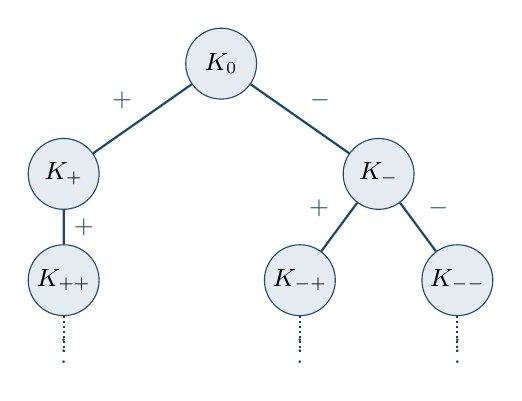
\begin{tikzpicture}[>=Latex,font=\small,
 cnode/.style={circle,draw=manifoldblue!80!black,
 fill=manifoldblue!12,minimum size=9mm,inner sep=1pt}]
 \node[cnode] (r) at (0,2.75) {$K_0$};
 \node[cnode] (a) at (-2,1.35) {$K_+$};
 \node[cnode] (b) at (2,1.35) {$K_-$};
 \node[cnode] (c) at (-2,0) {$K_{++}$};
 \node[cnode] (d) at (1,0) {$K_{-+}$};
 \node[cnode] (e) at (3,0) {$K_{--}$};
 \draw[manifoldblue!80!black,thick]
   (r)--node[above left] {$+$} (a)
   (r)--node[above right] {$-$} (b)
   (a)--node[right] {$+$} (c)
   (b)--node[above left] {$+$} (d)
   (b)--node[above right] {$-$} (e);
 \foreach \x in {c,d,e}{
   \draw[manifoldblue!65!black,densely dotted,thick]
      (\x.south)--++(0,-.45);
 }
 \node[manifoldblue!75!black] at (-2,-.8) {$\vdots$};
 \node[manifoldblue!75!black] at (1,-.8) {$\vdots$};
 \node[manifoldblue!75!black] at (3,-.8) {$\vdots$};
\end{tikzpicture}
\caption{Pierwsze trzy poziomy drzewa. $K_0$ ma
dwa załamania o znakach $+$ i $-$; dlatego w drugim
piętrze są dwa uchwyty. Ich załamania wyznaczają
trzecie piętro. Kropki oznaczają dalsze poziomy,
a nie końcowe wierzchołki.}
\label{fig:casson-signed-tree}
\end{figure}

\begin{przyklad}[Jedna gałąź]
\label{prz:casson-ray}
Jeśli każdy uchwyt ma dokładnie jedno dodatnie
załamanie, drzewo jest nieskończonym promieniem
ze wszystkimi znakami $+$. Każde piętro $T_n$
ma na szczycie jedną pętlę. Zmiana jednego znaku
nie zmienia tego prostego rachunku grupy podstawowej,
choć zmienia dane gładkich plumbowań.
\end{przyklad}

\begin{stwierdzenie}[Co dają skończone piętra]
\label{prop:casson-tower-pi1}
Niech $r_n$ oznacza liczbę punktów podwójnych
na $n$-tym piętrze. Wtedy
$\pi_1(T_n)$ jest grupą wolną na $r_n$ generatorach,
a homomorfizm
$\pi_1(T_n)\to\pi_1(T_{n+1})$ jest zerowy.
W szczególności $\pi_1(CH)=0$.
\end{stwierdzenie}
\begin{proof}
Dla $T_1$ jest to
Stwierdzenie~\ref{prop:casson-first-pi1}.
Załóżmy, że generatory $\pi_1(T_n)$ są pętlami
odpowiadającymi załamaniom najwyższego piętra.
Okrąg przyczepienia każdego nowego uchwytu
reprezentuje dokładnie jeden z tych generatorów.
W nowym uchwycie ten okrąg jest brzegiem jego
immersyjnego rdzenia, a więc staje się
nullhomotopijny. Twierdzenie van Kampena usuwa
wszystkie stare generatory. Pozostają wolne
generatory utworzone przez załamania nowych
uchwytów; ich liczba wynosi $r_{n+1}$.
To kończy indukcję. Każda pętla w $CH$ ma zwarty
obraz, mieści się więc w pewnym $T_n$ i staje się
nullhomotopijna w $T_{n+1}$.
\end{proof}

Ten rachunek nie stwierdza, że $CH$ jest standardowym
otwartym uchwytem $2$. Sama grupa podstawowa nie
rozpoznaje zachowania przy końcu niezwartym ani
lokalnej płaskości ewentualnego dysku granicznego.

\section{Dyski Whitneya i dane w pierścieniu grupowym}
\label{sec:casson-whitney}

Na Rysunku~\ref{fig:freedman-whitney} widzieliśmy
parę punktów przecięcia o znakach $+$ i $-$.
Jeśli odpowiedni okrąg Whitneya jest
nullhomotopijny, można go wypełnić immersyjnym
dyskiem. Ruch Whitneya usuwa wyjściową parę,
gdy wnętrze tego dysku jest czyste i obramowanie
jest właściwe. W wymiarze cztery wnętrze może
przeciąć powierzchnie, a sam dysk może przeciąć
siebie. Przeniesienie problemu na następny dysk
jest ideą wspólną wieżom Cassona i konstrukcjom
z dyskami Whitneya. Są to różne modele geometryczne:
w klasycznej wieży Cassona następne rdzenie
dołącza się do pętli pojedynczych załamań, nie
po prostu do każdej pary punktów Whitneya.

Przy nietrywialnej $\pi_1(M)$ same znaki przecięć
nie wystarczają nawet do znalezienia okręgu
Whitneya, który można wypełnić. Dla dwóch
zorientowanych, obramowanych immersyjnych dysków
lub sfer $A,B$ wybieramy ścieżki od ustalonego
punktu bazowego do ich obrazów. Punkt
$p\in A\cap B$ daje znak $\varepsilon_p\in\{+1,-1\}$
i element $g_p\in\pi_1(M)$: idziemy do $A$,
po $A$ do $p$, a następnie wracamy po $B$.
Otrzymujemy liczbę przecięcia z wartościami w
pierścieniu grupowym
\begin{equation}\label{eq:casson-lambda}
 \lambda(A,B)=\sum_{p\in A\cap B}
             \varepsilon_p g_p\in\Z[\pi_1(M)].
\end{equation}
Przy samoprzecięciu wybór kolejności dwóch płatów
zmienia $g$ na $g^{-1}$. Dlatego obramowana
liczba samoprzecięcia $\mu(B)$ należy do
addytywnego ilorazu
$\Z[\pi_1(M)]/\langle g-g^{-1}:g\in\pi_1(M)\rangle$.
Jest to \emph{niezredukowana} liczba samoprzecięcia:
zachowuje ją homotopia regularna. Dalsze podzielenie
przez podgrupę $\Z\cdot 1$ daje zredukowaną liczbę
\[
 \widetilde\mu(B)\in
 \Z[\pi_1(M)]/
 \bigl(\langle g-g^{-1}:g\in\pi_1(M)\rangle
       +\Z\cdot1\bigr),
\]
która zależy tylko od klasy homotopii. Lokalna
homotopia tworząca lub usuwająca pojedynczy punkt
podwójny z etykietą $1$ zmienia $\mu$, lecz nie
$\widetilde\mu$. Rozróżnienie to będzie istotne przy
porównaniu dwóch wersji twierdzenia o zanurzaniu.
Zależność od orientacji i obramowania oraz definicję
ogólną podają
\href{https://archive.mpim-bonn.mpg.de/4789/2/FreedmanQuinn-TopologyOf4Manifolds-Reformatted2013.pdf}
{Freedman--Quinn, \emph{Topology of 4-Manifolds},
\S\,1.7--1.8}. W przypadku $\pi_1(M)=0$
wartości~\eqref{eq:casson-lambda} są po prostu
całkowitymi liczbami przecięcia.

\begin{stwierdzenie}[Algebraiczne pary punktów]
\label{prop:casson-pairing}
Jeżeli $\lambda(A,B)=0$, punkty $A\cap B$ można
sparować tak, aby w każdej parze znaki były
przeciwne, elementy $g_p$ jednakowe, a okrąg
Whitneya był nullhomotopijny w $M$. Jeżeli
$\lambda(A,B)=1$, po takim parowaniu pozostaje
jeden dodatni punkt o etykiecie $1\in\pi_1(M)$.
\end{stwierdzenie}
\begin{proof}
Pierścień grupowy jest wolną grupą abelową z bazą
$\pi_1(M)$. Zatem współczynnik każdego $g$
w sumie~\eqref{eq:casson-lambda} znika osobno,
z wyjątkiem współczynnika $1$ w drugim przypadku.
Kojarzymy dodatnie i ujemne punkty o tej samej
etykiecie. Dla takiej pary wybieramy łuk od
pierwszego punktu do drugiego na $A$ i łuk
powrotny na $B$. Definicja $g_p$ pokazuje,
że klasa otrzymanej pętli jest iloczynem
$g_p g_q^{-1}=1$. Pętla jest więc nullhomotopijna.
Jej wypełnienie można doprowadzić do położenia
ogólnego jako \emph{immersyjny} dysk Whitneya;
ten ostatni krok nie usuwa jego przecięć wewnętrznych.
\end{proof}

Analogiczna implikacja dla $\mu(B)=0$ wymaga
uwzględnienia zamiany płatów i opisanej relacji
$g\sim g^{-1}$; zob.
Freedman--Quinn, \S\,1.7. Obramowania też
nie można pominąć: skręcenie brzegu dysku
Whitneya może poprawić jego obramowanie,
ale zwykle wytwarza nowe przecięcie z jedną
z powierzchni. Ta algebraiczna redukcja daje
więc \emph{immersyjne} dyski; ich topologiczne
zanurzenie jest następnym, odrębnym krokiem.

\section{Twierdzenie o zanurzaniu dysku}
\label{sec:casson-disk-theorem}

Klasyczny uchwyt Cassona wystarcza w konstrukcji
jednospójnej. Dla nietrywialnej grupy podstawowej
Freedman--Quinn używają dodatkowo powierzchni z
dyskami zamykającymi i uogólnionych wież; warunek
grupowy służy do kontroli pętli punktów podwójnych.
Poniższe twierdzenie nie jest więc formalnym skutkiem
samego rachunku $\pi_1(CH)=0$ ani standardowości
pojedynczego klasycznego uchwytu Cassona.

Grupę $G$ nazywamy \emph{wielostopniowo skończoną
lub cykliczną} (ang. \emph{poly-(finite or cyclic)}),
jeśli ma skończony ciąg
$1=G_0\triangleleft G_1\triangleleft\cdots
\triangleleft G_m=G$, w którym każdy iloraz
$G_{i+1}/G_i$ jest skończony albo nieskończenie
cykliczny.
W szczególności należą tu grupa trywialna,
grupy skończone i $\Z^k$. Jest to konkretna
klasa grup użyta w poniższej wersji twierdzenia.

\begin{twierdzenie}[Freedman--Quinn: zanurzanie dysków;
wynik zewnętrzny]
\label{thm:casson-disk-embedding}
Niech $M^4$ będzie zwartą, spójną, zorientowaną gładką
rozmaitością z brzegiem, a
$A_i:(D^2,S^1)\to(M,\partial M)$,
$1\leq i\leq r$, skończoną rodziną właściwych
immersji obramowanych dysków. Ich brzegi
są parami rozłącznie zanurzone wraz z kołnierzami.
Załóżmy, że istnieją obramowane immersyjne sfery
$B_j:S^2\to\operatorname{int}M$ takie, że w
$\Z[\pi_1(M)]$ zachodzą
\begin{equation}\label{eq:casson-duals}
 \lambda(A_i,B_j)=\delta_{ij},\qquad
 \lambda(B_i,B_j)=0,
\end{equation}
a w grupie samoprzecięć zachodzi $\mu(B_j)=0$
dla każdego $j$. Jeśli $\pi_1(M)$ jest
wielostopniowo skończona lub cykliczna, to w $M$
istnieją parami rozłączne, lokalnie płasko
\emph{topologicznie zanurzone} dyski o tych samych
obramowanych brzegach. Mają one obramowane immersyjne
sfery $B'_j$, homotopijne odpowiednio do $B_j$,
które są geometrycznie dualne: każda $B'_j$ przecina
odpowiedni dysk w jednym punkcie i jest rozłączna
z pozostałymi dyskami.
\end{twierdzenie}

Sfery $B_j$ są \emph{algebraicznie dualne} do
dysków: pierwsza równość w~\eqref{eq:casson-duals}
oznacza jeden punkt przecięcia po skasowaniu
algebraicznych par. Pozostałe warunki kontrolują
przecięcia samych sfer. Obramowanie oznacza tu
trywializację dwuwymiarowej wiązki normalnej,
zgodną z zadanym obramowaniem brzegów dysków.
Twierdzenie podajemy za
\href{https://archive.mpim-bonn.mpg.de/4789/2/FreedmanQuinn-TopologyOf4Manifolds-Reformatted2013.pdf}
{Freedman--Quinn, \emph{Topology of 4-Manifolds},
Twierdzenie 5.2, s.\ 85--87}; w wydaniu książkowym
z 1990 roku jest to Twierdzenie 5.1A. Wersja dla gładkiego
$M$ unika dodatkowego przejścia od rozmaitości
topologicznej do gładkich lokalnych modeli
immersji; to przejście autorzy omawiają
w rozdziale 9. Konkluzja pozostaje topologiczna.
Twierdzenie samo nie mówi, że wyjściowe immersje $A_i$
są homotopijne regularnie do uzyskanych zanurzeń.

W konkluzji słowo \emph{poprzeczne} ma znaczenie
geometryczne: każda uzyskana sfera przecina swój
dysk w dokładnie jednym punkcie, a pozostałe dyski
omija. Samo równanie
$\lambda(A_i,B_j)=\delta_{ij}$ jest słabsze, bo
dopuszcza dodatkowe pary przecięć. W oryginalnym
dowodzie Freedmana--Quinna przejście od dualności
algebraicznej do takich sfer zawierało lukę. Domyka
ją \href{https://arxiv.org/pdf/2006.05209}
{Powell--Ray--Teichner, \emph{The 4-dimensional disc
embedding theorem and dual spheres} (2025),
Twierdzenie A i \S\,5}. Twierdzenie A obejmuje
przytoczoną wyżej wersję dla gładkiego $M$ i grup
wielostopniowo skończonych lub cyklicznych. Jest
sformułowane za pomocą $\widetilde\mu$ i dowolnych
grup dobrych; nasze założenie obramowania oraz
$\mu(B_j)=0$ jest mocniejszym przypadkiem. Nowe
źródło daje sfery $B'_j$ w klasach homotopii $B_j$.
Samo istnienie
zanurzonych dysków wynikało już z wcześniejszej
części argumentu Freedmana--Quinna. Nowe źródło
uzasadnia dodatkową, używaną dalej konkluzję
o \emph{geometrycznie} dualnych sferach.

\begin{stwierdzenie}[Co zapewnia geometryczna dualność]
\label{prop:casson-complement-pi1}
Niech $D_1,\ldots,D_r$ będą parami rozłącznymi,
lokalnie płasko zanurzonymi właściwymi dyskami w
zwartej spójnej rozmaitości $M^4$ z brzegiem.
Jeżeli mają geometrycznie
dualne immersyjne sfery, to inkluzja dopełnienia
indukuje izomorfizm
\[
 \pi_1\bigl(M\setminus\textstyle\bigcup_i D_i\bigr)
       \xrightarrow{\ \cong\ }\pi_1(M).
\]
\end{stwierdzenie}

Jest to własność $\pi_1$-pomijalności wyróżniona w
\href{https://arxiv.org/pdf/2006.05209}
{Powell--Ray--Teichner, Uwaga 1.2}.
\begin{proof}
Przez położenie ogólne każdą pętlę w $M$ można
odsunąć od dysków, więc homomorfizm jest
surjektywny. Niech pętla w dopełnieniu ogranicza
dysk odwzorowany w $M$. Korzystamy tu z
topologicznej transwersalności dla lokalnie
płaskich podrozmaitości oraz z reprezentowania
klas map przez generyczne immersje,
\href{https://arxiv.org/pdf/2006.05209}
{Powell--Ray--Teichner, Twierdzenia 6.4 i 1.5}.
Po uczynieniu odwzorowania poprzecznym do $D_i$
przeciwobrazy
dysków są skończonym zbiorem punktów. Usuwamy
małe kółka wokół tych punktów. Pozostała część
dysku leży w dopełnieniu, a każdy nowy okrąg
brzegowy jest meridianem jednego z $D_i$.
Sfera dualna do $D_i$, po usunięciu małego krążka
otaczającego jej jedyny punkt przecięcia z $D_i$,
daje immersyjny dysk w dopełnieniu, którego brzeg
jest takim meridianem. Wszystkie meridiany są
zatem nullhomotopijne w dopełnieniu, także po
sprzężeniu ścieżkami potrzebnymi do zmiany punktu
bazowego. Doklejenie tych immersyjnych dysków
wypełnia wyjściową pętlę w dopełnieniu. Homomorfizm
jest więc także injektywny.
\end{proof}

Ten prosty skutek wyjaśnia, dlaczego nie wystarcza
zastąpić w konkluzji twierdzenia dualności
geometrycznej dualnością algebraiczną: w drugim
przypadku sfera może mieć kilka punktów przecięcia
z dyskiem, a powyższe wypełnienie meridianu nie
powstaje. Jest to również powód, dla którego
\href{https://arxiv.org/pdf/2006.05209}
{Powell--Ray--Teichner, Uwaga 1.2} podkreślają
kontrolę grupy podstawowej dopełnienia.

\begin{przyklad}[Standardowa para dualna]
\label{prz:casson-dual-product}
Weźmy $M=S^2\times D^2$,
$A=\{p\}\times D^2$ i $B=S^2\times\{0\}$.
Wtedy $\pi_1(M)=0$, dysk i sfera przecinają się
w jednym dodatnim punkcie, $\lambda(A,B)=1$,
a $\mu(B)=0$. Normalne kierunki do obu czynników
dają wymagane obramowania. Twierdzenie obejmuje
tę parę, chociaż tutaj $A$ jest już zanurzony.
Jeżeli $A$ zmienimy we wnętrzu lokalnym ruchem
palcowym, jego brzeg i dualność
algebraiczna nadal pozostają takie same;
nowe punkty podwójne pokazują, jak wyglądają
dane przed zastosowaniem twierdzenia.
\end{przyklad}

\begin{wniosek}[Wersja z homotopią regularną;
wynik zewnętrzny]
\label{cor:casson-regular-homotopy}
Przy założeniach Twierdzenia~\ref{thm:casson-disk-embedding}
załóżmy dodatkowo, że wszystkie algebraiczne
przecięcia wzajemne $A_i$ oraz ich liczby
samoprzecięcia $\mu(A_i)$ są zerowe.
Wtedy rodzinę $A_i$ można przez homotopię
regularną względnie brzegów doprowadzić do
parami rozłącznych topologicznie zanurzonych
dysków z dualnymi sferami.
\end{wniosek}

To jest \href{https://archive.mpim-bonn.mpg.de/4789/2/FreedmanQuinn-TopologyOf4Manifolds-Reformatted2013.pdf}
{Freedman--Quinn, Wniosek 5.2.1, s.\ 87--88};
w wydaniu książkowym jest to Wniosek 5.1B.
Dodatkowych równości dotyczących $A_i$ nie
ukrywamy w Twierdzeniu~\ref{thm:casson-disk-embedding}:
tam potrzebne jest jedynie zachowanie
obramowanych brzegów.

Warto rozdzielić pośrednie kroki tego wniosku.
Równości $\lambda(A_i,A_j)=0$ i $\mu(A_i)=0$
parują algebraicznie przecięcia dysków i pozwalają
wybrać \emph{immersyjne}, odpowiednio obramowane
dyski Whitneya. Najpierw ruchy Whitneya
z użyciem tych dysków
redukują dodatkowe przecięcia $A_i$ ze sferami
algebraicznie dualnymi. Następnie z torusów
opasujących punkty podwójne oraz sfer dualnych
buduje się sfery algebraicznie dualne do samych
dysków Whitneya. Do \emph{nich} stosuje się
Twierdzenie~\ref{thm:casson-disk-embedding},
otrzymując rozłączne zanurzone dyski Whitneya.
Prowadzone po nich ruchy Whitneya usuwają
przecięcia $A_i$; ponieważ są to ruchy wewnątrz,
zachowują obramowane brzegi i dają wskazaną
homotopię regularną. Konstrukcja sfer dualnych
do dysków Whitneya jest częścią zewnętrznego
dowodu Freedmana--Quinna, s.\ 87--88; nie wynika
z samego parowania w pierścieniu grupowym.
Warunek $\mu(A_i)=0$ dotyczy tu niezredukowanej
liczby: właśnie on wyklucza konieczność homotopii
tworzących pojedyncze punkty z etykietą $1$ i pozwala
otrzymać homotopię regularną, a nie tylko dowolną.

Inny ważny znany zakres wyniku stanowią grupy o
wzroście podwykładniczym. Grupa skończenie generowana
ma \emph{wzrost podwykładniczy}, jeśli dla pewnego ---
a równoważnie dla każdego --- skończonego symetrycznego
zbioru generatorów $S$
liczba elementów o długości co najwyżej $n$
spełnia $\lim_{n\to\infty}|B_S(n)|^{1/n}=1$.
Ta własność obejmuje w szczególności grupy
o wzroście wielomianowym. Dla grup podstawowych
o wzroście podwykładniczym tę samą konkluzję
zanurzania otrzymuje się dzięki ulepszeniu
kontroli pętli punktów podwójnych; zob.
\href{https://math.berkeley.edu/~teichner/Papers/Freedman1.pdf}
{Freedman--Teichner, \emph{4-Manifold topology I:
Subexponential groups} (1995)} oraz
\href{https://uva.theopenscholar.com/files/slava-krushkal/files/subexponential_groups.pdf}
{Krushkal--Quinn, \emph{Subexponential groups in
4-manifold topology} (2000)}. Ostatnia praca
podaje poprawiony argument i wskazuje błąd
w pierwotnym dowodzie z 1995 roku. Nie
rozszerzamy stąd twierdzenia na dowolną grupę
podstawową. Jest również wersja z dowolną
$\pi_1(M)$ przy silnym \emph{geometrycznym}
założeniu $\pi_1$-zerowości poprzecznych
powierzchni z dyskami zamykającymi
(Freedman--Quinn, Twierdzenie 5.4).

\section{Gdzie kończy się redukcja geometryczna}
\label{sec:casson-boundary}

Możemy teraz uporządkować rzeczywiście wykonane
kroki. Zerowanie współczynników pierścienia
grupowego pozwala sparować punkty przecięcia
i znaleźć immersyjne dyski Whitneya
(Stwierdzenie~\ref{prop:casson-pairing}).
Samoplumbowanie daje uchwyt pierwszego
piętra z podpisanym znakiem każdego punktu
podwójnego. Dołączanie kolejnych pięter zabija
generatory grupy podstawowej powstałe na
poprzednim piętrze
(Stwierdzenie~\ref{prop:casson-tower-pi1}).
Żaden z tych skończonych rachunków nie produkuje
jeszcze dysku o czystym wnętrzu.

W dowodzie Twierdzenia~\ref{thm:casson-disk-embedding}
potrzeba ponadto skonstruować powierzchnie z
dyskami zamykającymi i dualne sfery, poprawić
grupę podstawową pętli punktów podwójnych,
otrzymać zbieżną wieżę oraz zanurzyć dysk
lokalnie płasko w jej otoczeniu. Są to zasadnicze
zewnętrzne części teorii Freedmana--Quinna:
\href{https://archive.mpim-bonn.mpg.de/4789/2/FreedmanQuinn-TopologyOf4Manifolds-Reformatted2013.pdf}
{\emph{Topology of 4-Manifolds}, rozdziały 2--5}.
Ostatnie przejście opiera się na kontroli
topologicznej przy nieskończonym końcu wieży;
nie wynika z samego van Kampena ani z formalnej
granicy ciągu ruchów Whitneya.

\begin{twierdzenie}[Freedman: standardowość topologiczna
uchwytu Cassona; wynik zewnętrzny]
\label{thm:casson-homeomorphism}
Każdy uchwyt Cassona wraz ze swym obszarem
przyczepienia jest homeomorficzny jako para ze
standardowym otwartym uchwytem $2$:
\[
 (CH,\partial_-CH)\cong
 (D^2\times\R^2,S^1\times\R^2).
\]
Homeomorfizm można dobrać zgodnie z ustalonym
obramowaniem obszaru przyczepienia.
\end{twierdzenie}

Jest to \href{https://www.maths.gla.ac.uk/~mpowell/1982_The%20topology%20of%20four-dimensional%20manifolds.pdf}
{Freedman, \emph{The topology of four-dimensional
manifolds} (1982), Twierdzenie 1.1}.
Przyjmujemy je tutaj jako wynik zewnętrzny.
Jego dowód wymaga ponownego zanurzania wież,
kontroli zbiorów granicznych i argumentów
zmniejszania rozkładów topologicznych. Dopiero
ten wynik uzasadnia przejście od uchwytu Cassona
do standardowego otwartego uchwytu w kategorii
TOP. Nie daje analogicznego dyfeomorfizmu par
w kategorii gładkiej. W szczególności topologiczny
rdzeń $D^2\times\{0\}$ nie musi być gładkim
zanurzonym dyskiem w pierwotnym gładkim $M$.

Twierdzenie o zanurzaniu dysku jest geometrycznym
narzędziem stojącym za topologicznymi wnioskami
Freedmana przytoczonymi w
rozdziale~\ref{ch:freedman-formy}. Wnioski o
gładkich strukturach wymagają osobnych przeszkód;
same znakowane drzewa, wyzerowanie $\pi_1(CH)$
i lokalna płaskość topologiczna ich nie rozstrzygają.

\par\smallskip
{\footnotesize\noindent\emph{Dalsza lektura:}
\href{https://archive.mpim-bonn.mpg.de/4789/2/FreedmanQuinn-TopologyOf4Manifolds-Reformatted2013.pdf}
{M.\ H.\ Freedman i F.\ Quinn, \emph{Topology of 4-Manifolds}},
rozdziały 2--5: uchwyty Cassona i twierdzenie o zanurzaniu dysku;
\href{https://arxiv.org/pdf/2006.05209}
{M.\ Powell, A.\ Ray i P.\ Teichner, \emph{The 4-dimensional
disc embedding theorem and dual spheres}}, korekta argumentu
o sferach dualnych.\par}

\chapter{Klasyfikacja topologicznych rozmaitości czterowymiarowych}
\label{ch:freedman-klasyfikacja}
\index{Freedman!klasyfikacja wymiaru cztery}

W Rozdziale~\ref{ch:freedman-formy} obliczaliśmy formy
przecięcia i oglądaliśmy przeszkodę dla gładkiego
triku Whitneya. Uchwyty Cassona, opisane w
Rozdziale~\ref{ch:uchwyty-cassona}, stanowią drogę
do topologicznego twierdzenia o zanurzaniu dysku.
Poniżej podamy precyzyjny wynik klasyfikacyjny
Freedmana jako wejście zewnętrzne i wyprowadzimy
z niego wnioski. Każde stwierdzenie o homeomorfizmie
dotyczy kategorii TOP; typy gładkie wymagają
osobnych argumentów.

\section{Niezmiennik Kirby'ego--Siebenmanna}
\label{sec:freedman-ks}
\index{niezmiennik Kirby'ego--Siebenmanna}

Niech $X$ będzie zamkniętą, spójną, topologiczną
rozmaitością $4$-wymiarową. Jej stabilna wiązka
styczna jest w kategorii TOP mikrowiązką. Teoria
Kirby'ego--Siebenmanna przypisuje jej klasę
\begin{equation}\label{eq:freedman-ks}
 \operatorname{ks}(X)\in H^4(X;\Z/2).
\end{equation}
Po ewaluacji na mod $2$ klasie fundamentalnej
otrzymujemy liczbę w $\Z/2$, również oznaczaną
$\operatorname{ks}(X)$. Intuicyjnie mierzy ona
przeszkodę do \emph{stabilnego} wygładzenia: dla
zamkniętej rozmaitości $4$-wymiarowej
$\operatorname{ks}(X)=0$ wtedy i tylko wtedy,
gdy $X\times\R$ dopuszcza strukturę gładką.
Jest to wynik zewnętrzny teorii wygładzania,
\href{https://archive.mpim-bonn.mpg.de/4789/2/FreedmanQuinn-TopologyOf4Manifolds-Reformatted2013.pdf}
{Freedman--Quinn, \S\,8.7--8.8 i \S\,10.2.2},
oparty na
\href{https://www.maths.ed.ac.uk/~v1ranick/papers/ks.pdf}
{Kirby--Siebenmann, \emph{Foundational Essays on
Topological Manifolds, Smoothings, and Triangulations}
(1977)}.

W szczególności struktura gładka lub PL na $X$
wymusza $\operatorname{ks}(X)=0$. W wymiarze cztery
odwrotnej implikacji \emph{nie} wolno wyciągać z
tego twierdzenia: zerowanie przeszkody stabilnej
nie buduje automatycznie wygładzenia samego $X$.
Niezmiennik jest zachowywany przez homeomorfizmy,
a dla sum spójnych zachodzi
\[
 \operatorname{ks}(X\#Y)
   =\operatorname{ks}(X)+\operatorname{ks}(Y)
       \quad\text{w }\Z/2.
\]
Te własności również przyjmujemy z powyższego źródła.

Jeżeli $X$ jest dodatkowo jednospójna i zorientowana,
parzystość $Q_X$ odpowiada warunkowi
$w_2(X)=0$: jest to wzór Wu
$Q_X(x,x)\equiv\langle w_2(X),x\rangle\pmod2$
wraz z brakiem $2$-torsji w $H_1(X)$.
Jest to topologiczna wersja warunku spinowego;
również ją przyjmujemy jako wynik zewnętrzny,
\href{https://archive.mpim-bonn.mpg.de/4789/2/FreedmanQuinn-TopologyOf4Manifolds-Reformatted2013.pdf}
{Freedman--Quinn, \S\,10.2.1--10.2.2}.
Bez hipotezy o $H_1$ sama parzystość formy na
całkowitej homologii nie musi wykrywać całego $w_2$.

\section{Twierdzenie Freedmana jako wynik zewnętrzny}
\label{sec:freedman-classification}

\begin{twierdzenie}[Freedman: klasyfikacja jednospójna;
wynik zewnętrzny]
\label{thm:freedman-classification}
Niech $Q$ będzie symetryczną unimodularną formą
całkowitą na wolnej grupie abelowej skończonej rangi,
a $k\in\Z/2$. Jeśli $Q$ jest parzysta, załóżmy
dodatkowo
\begin{equation}\label{eq:freedman-even-ks}
 k\equiv\frac{\sigma(Q)}8\pmod2.
\end{equation}
Wtedy istnieje zamknięta, spójna, zorientowana,
jednospójna \emph{topologiczna} rozmaitość
$X^4$ z $Q_X\cong Q$ i $\operatorname{ks}(X)=k$.
Jeśli $Q$ jest nieparzysta, obie wartości $k=0,1$
są dopuszczalne.

Ponadto dwie takie rozmaitości są homeomorficzne
z zachowaniem orientacji wtedy i tylko wtedy,
gdy ich formy przecięcia są izometryczne i mają
ten sam niezmiennik Kirby'ego--Siebenmanna.
W wersji z ustaloną izometrią form homeomorfizm
można wybrać tak, by indukował właśnie tę izometrię.
\end{twierdzenie}

Wzór~\eqref{eq:freedman-even-ks} ma sens, ponieważ
sygnatura parzystej formy unimodularnej jest podzielna
przez $8$; jak zaznaczono po
Stwierdzeniu~\ref{prop:freedman-E8-properties},
ogólny fakt algebraiczny przyjmujemy z literatury.
Dla jednospójnej $X$ parzystość $Q_X$ oznacza także
$w_2(X)=0$, więc $X$ jest spinowa. W tym przypadku
zewnętrzna formuła dla zamkniętych topologicznych
rozmaitości spinowych brzmi
$\operatorname{ks}(X)\equiv\sigma(X)/8\pmod2$;
zob. Freedman--Quinn, \S\,10.2.2. Wyjaśnia ona
konieczność warunku~\eqref{eq:freedman-even-ks},
natomiast część istnienia Twierdzenia~\ref{thm:freedman-classification}
zapewnia jego wystarczalność.
Oryginalne Twierdzenie 1.5 w pracy
\href{https://www.maths.gla.ac.uk/~mpowell/1982_The%20topology%20of%20four-dimensional%20manifolds.pdf}
{M.\ H.\ Freedman, \emph{The topology of four-dimensional
manifolds}, J. Differential Geom. 17 (1982), 357--453}
jest sformułowane dla rozmaitości gładkich poza jednym
punktem. Podaną wyżej pełną postać w kategorii TOP,
razem z warunkiem na $\operatorname{ks}$, przyjmujemy z
\href{https://archive.mpim-bonn.mpg.de/4789/2/FreedmanQuinn-TopologyOf4Manifolds-Reformatted2013.pdf}
{M.\ H.\ Freedman i F.\ Quinn, \emph{Topology of
4-Manifolds}, \S\,10.1}.
W źródłach dowód korzysta z topologicznego zanurzania
dysków i uchwytów Cassona. Poprzednie sekcje tego
rozdziału nie dowodzą istnienia ani jednoznaczności
homeomorfizmu z twierdzenia.

\section{Dwie konstrukcje w dowodzie Freedmana}
\label{sec:freedman-constructive-examples}
\index{Freedman!konstrukcja rozmaitości o formie $E_8$}

Twierdzenie~\ref{thm:freedman-classification} jest
wynikiem zewnętrznym, ale jego pierwszą konstrukcję
możemy prześledzić na obliczonym już plumbowaniu.
Oddzielimy rachunki homologii i formy od istnienia
topologicznego wypełnienia brzegu. Drugą konstrukcją
będzie rozmaitość o formie $[1]$, której nie da się
odróżnić od $\C P^2$ samą formą przecięcia.

\begin{przyklad}[Od plumbowania do $X_{E_8}$]
\label{prz:freedman-E8-gluing}
Niech $P$ będzie plumbowaniem ośmiu zorientowanych
wiązek $D^2\to P_i\to S^2$ o liczbie Eulera $+2$.
Ich rdzenie są sferami o samoprzecięciu $+2$;
plumbowania wykonujemy według grafu z
Rysunku~\ref{fig:freedman-E8-graph}, wybierając
znaki przecięć sąsiednich rdzeni równe $-1$.
Równoważnie $P$ otrzymujemy z $D^4$ przez osiem
uchwytów $2$ o macierzy sprzężeń $E_8$.
Nie ma uchwytów $1$, zatem $\pi_1(P)=1$, a
Stwierdzenie~\ref{prop:freedman-link-matrix} daje
\[
 H_2(P;\Z)\cong\Z^8,\qquad Q_P=E_8,
 \qquad H_1(\partial P;\Z)=H_2(\partial P;\Z)=0.
\]
Ostatnia równość korzysta z
$\det E_8=1$ ze Stwierdzenia~\ref{prop:freedman-E8-properties}.
Brzeg $\Sigma=\partial P$ jest więc całkowitą
sferą homologiczną. Według Freedmana--Quinna jest
to sfera homologiczna Poincarégo z odpowiednią
orientacją; sam rachunek homologii nie identyfikuje
jej jako $S^3$.

Głęboki krok pochodzi z twierdzenia Freedmana:
\emph{każda} całkowita sfera homologiczna wymiaru
trzy ogranicza kontraktowalną topologiczną
rozmaitość $4$-wymiarową. Wybierzmy takie $C$
z $\partial C\cong-\Sigma$ i sklejmy
\[
 X_{E_8}=P\cup_{\Sigma}C.
\]
Istnienie $C$ jest wynikiem zewnętrznym,
\href{https://www.maths.gla.ac.uk/~mpowell/1982_The%20topology%20of%20four-dimensional%20manifolds.pdf}
{Freedman, \emph{The topology of four-dimensional
manifolds}, twierdzenie $1.4'$}; zob. też
\href{https://archive.mpim-bonn.mpg.de/4789/2/FreedmanQuinn-TopologyOf4Manifolds-Reformatted2013.pdf}
{Freedman--Quinn, wniosek 9.7.2 i \S\,10.5.1}.

Pozostałe kroki są już rachunkami. Twierdzenie
van Kampena opisuje $\pi_1(X_{E_8})$ jako iloraz
$\pi_1(P)*\pi_1(C)$ przez relacje pochodzące od
$\pi_1(\Sigma)$. Oba czynniki są trywialne, bo
$P$ jest jednospójne, a $C$ kontraktowalne;
stąd $\pi_1(X_{E_8})=1$.
Fragment ciągu Mayera--Vietorisa ma postać
\[
 0=H_2(\Sigma;\Z)\longrightarrow
 H_2(P;\Z)\oplus H_2(C;\Z)
 \longrightarrow H_2(X_{E_8};\Z)
 \longrightarrow H_1(\Sigma;\Z)=0.
\]
Ponieważ $H_2(C)=0$, inkluzja $P\hookrightarrow X_{E_8}$
indukuje izomorfizm na $H_2$. Sfery zerowe
plumbowanych wiązek reprezentują bazę $H_2(P)$
i przecinają się we wnętrzu $P$, więc po sklejeniu
zachowują macierz $E_8$. Otrzymaliśmy zatem
zamkniętą, jednospójną rozmaitość topologiczną
o $Q_{X_{E_8}}=E_8$ i $\sigma(X_{E_8})=8$.
Forma jest parzysta, więc $X_{E_8}$ jest spinowa;
zewnętrzny wzór z Sekcji~\ref{sec:freedman-ks}
daje $\operatorname{ks}(X_{E_8})=8/8=1\pmod2$.
To obliczenie wyklucza wygładzenie $X_{E_8}$.
Nie dostarcza ono samodzielnej konstrukcji $C$.
\end{przyklad}

\begin{przyklad}[Drugi typ o formie nieparzystej rzędu jeden]
\label{prz:freedman-odd-twin}
\index{Freedman!drugi typ o formie $[1]$}
Rozważmy $Z=X_{E_8}\#\overline{\C P^2}$. Addytywność
formy i niezmiennika Kirby'ego--Siebenmanna daje
\[
 Q_Z=E_8\oplus[-1],\qquad
 \operatorname{ks}(Z)=1.
\]
Forma $Q_Z$ ma rząd $9$, sygnaturę $7$, jest
nieparzysta i nieokreślona. Klasyfikacja całkowitych
nieparzystych form nieokreślonych daje izometrię
\[
 E_8\oplus[-1]\cong8[1]\oplus[-1].
\]
Jest to twierdzenie algebraiczne cytowane przez
Freedmana--Quinna w \S\,10.2.1; jawny rachunek
odpowiedniej bazy, po odwróceniu znaków, znajduje się
również w Rozdziale~\ref{ch:egzotyczne-r4}.

Wybierzmy w tej izometrii podformę
$7[1]\oplus[-1]$, realizowaną przez gładką
rozmaitość $M=7\C P^2\#\overline{\C P^2}$.
Jej dopełnienie ortogonalne ma formę $[1]$,
na której $w_2$ jest niezerowa, bo kwadrat
generatora jest nieparzysty. Freedman--Quinn
sprawdzają w tym jednospójnym przypadku
pozostałe warunki dotyczące przecięć
i samoprzecięć. Ich zewnętrzne
\emph{twierdzenie o rozkładzie sumy spójnej}
pozwala zrealizować tę podformę jako rozkład
\[
 Z\cong M\#N,\qquad Q_N=[1].
\]
Właśnie ten krok, a nie sama izometria kratek,
korzysta z głębokiej geometrii wymiaru cztery;
zob. \href{https://archive.mpim-bonn.mpg.de/4789/2/FreedmanQuinn-TopologyOf4Manifolds-Reformatted2013.pdf}
{Freedman--Quinn, twierdzenie 10.4 i \S\,10.5.1
w numeracji wersji z 2013 r.}; w wydaniu z 1990 r.
są to twierdzenie 10.3 i dowód twierdzenia 10.1
w \S\,10.4.
Z addytywności otrzymujemy
$\operatorname{ks}(N)=\operatorname{ks}(Z)-
\operatorname{ks}(M)=1$, gdyż $M$ jest gładka.
Ponadto $N$ jest jednospójna na mocy twierdzenia
van Kampena dla sumy spójnej. Ma tę samą formę
$[1]$ co $\C P^2$, lecz inne $\operatorname{ks}$;
stąd nie jest z nią homeomorficzna i nie może
być gładka. Istnienie obu typów w nieparzystym
przypadku Twierdzenia~\ref{thm:freedman-classification}
ma więc konkretny punkt wyjścia w $X_{E_8}$.
\end{przyklad}

\section{Jak zanurzanie dysków wchodzi do klasyfikacji}
\label{sec:freedman-route}

W przypadku jednospójnym grupa podstawowa jest
trywialna, więc spełnia warunek
Twierdzenia~\ref{thm:casson-disk-embedding}.
Twierdzenie to zastępuje odpowiednio przygotowane
immersyjne dyski lokalnie płaskimi zanurzeniami, lecz
\emph{nie} klasyfikuje jeszcze rozmaitości: nie
konstruuje samo formy przecięcia, nie wyznacza
niezmiennika Kirby'ego--Siebenmanna i nie daje
homeomorfizmu między dwiema zadanymi rozmaitościami.

Pierwszym dalszym krokiem jest przejście od dysków
do sfer. W używanej tutaj szczególnej postaci
zewnętrzne \emph{twierdzenie o zanurzaniu sfer} mówi:
jeżeli w spójnej, zorientowanej topologicznej
rozmaitości $M^4$ z $\pi_1(M)=1$ mamy rodzinę obramowanych,
immersyjnych sfer $A_i$ z
$\lambda(A_i,A_j)=0$ dla $i\ne j$ i
$\mu(A_i)=0$, a także obramowane immersyjne sfery
algebraicznie dualne do $A_i$, to rodzinę $A_i$ można
przez homotopię regularną doprowadzić do parami
rozłącznych, lokalnie płasko zanurzonych obramowanych
sfer mających geometrycznie dualne immersyjne sfery.
W tej obramowanej postaci normalna liczba Eulera
$e(A_i)$ wynosi zero. Ponieważ $\pi_1(M)=1$,
to $\lambda(A_i,A_i)=2\mu(A_i)+e(A_i)=0$;
spełniony jest zatem warunek homotopii regularnej,
a zanurzone sfery mają trywialne wiązki normalne.
Jest to szczególny
przypadek \href{https://arxiv.org/pdf/2006.05209}
{Powell--Ray--Teichner, \emph{The 4-dimensional disc
embedding theorem and dual spheres} (2025),
Twierdzenie B i Uwaga 2.2}. W ogólnej postaci twierdzenie
rozróżnia zredukowaną liczbę samoprzecięć od
liczby Eulera normalnego i wymaga $w_2=0$ na
klasach sfer dualnych. Podane tutaj obramowanie
spełnia ten ostatni warunek.

Geometryczna dualność pozwala kontrolować
chirurgię na zanurzonych sferach. Dla jednej
obramowanej sfery $S$ usuwamy
$S^2\times\operatorname{int}D^2$ i wklejamy
$D^3\times S^1$ wzdłuż wspólnego
$S^2\times S^1$. Oznaczmy przez $C$ domknięcie
dopełnienia usuniętego otoczenia, a przez $m$
meridian $S$ w $\partial C$. Twierdzenie van
Kampena daje
\[
 \pi_1(M)\cong\pi_1(C)/\langle\!\langle m\rangle\!\rangle,
 \qquad
 \pi_1(M_{\mathrm{chir}})\cong\pi_1(C),
\]
ponieważ inkluzja $S^2\times S^1\hookrightarrow
D^3\times S^1$ indukuje izomorfizm grup
podstawowych. Gdy $S$ ma
geometrycznie dualną sferę, meridian ogranicza
w $C$ immersyjny dysk, dokładnie jak
w dowodzie Stwierdzenia~\ref{prop:casson-complement-pi1}.
Zatem $m=1$ w $\pi_1(C)$ i chirurgia zachowuje
grupę podstawową.
Jest to jeden z konkretnych powodów, dla których
wniosek o sferach dualnych w twierdzeniu o
zanurzaniu nie jest tylko dodatkiem do jego tezy.

Następne kroki są \emph{zewnętrzne}: algebraiczna
teoria chirurgii organizuje jądra przekształceń
normalnych w pary sfer do zanurzenia; topologiczna
chirurgia w wymiarze cztery używa tych zanurzeń
do usunięcia jądra; twierdzenie o $s$-kobordyzmie
w wymiarze pięć dla dobrej grupy podstawowej
(tu trywialnej) identyfikuje odpowiedni topologiczny
$s$-kobordyzm, którego inkluzje końców są prostymi
równoważnościami homotopijnymi, z produktem.
Dodatkowe argumenty istnienia rozmaitości
o zadanej formie oraz rachunek niezmiennika
Kirby'ego--Siebenmanna domykają klasyfikację.
Dokładne twierdzenia i ich hipotezy znajdują się
u \href{https://archive.mpim-bonn.mpg.de/4789/2/FreedmanQuinn-TopologyOf4Manifolds-Reformatted2013.pdf}
{Freedmana--Quinna, rozdziały 7, 10 i 11},
zwłaszcza Twierdzenie 7.2 oraz \S\,10.1 i \S\,11.6.
Powiązanie tych narzędzi wyjaśnia rolę
Twierdzenia~\ref{thm:casson-disk-embedding},
ale nie jest dowodem
Twierdzenia~\ref{thm:freedman-classification}.

Rysunek~\ref{fig:freedman-classification-route} zbiera
kolejność zależności dla przypadku $\pi_1=1$.
Sfery algebraicznie dualne są częścią danych wejściowych
twierdzenia o zanurzaniu; geometrycznie dualne sfery
są jego wnioskiem. Strzałki oznaczają użycie wyników
zewnętrznych z hipotezami podanymi wyżej, a nie
samodzielną konstrukcję klasyfikacji.

\begin{figure}[htbp]
\centering
\begin{tikzpicture}[
  font=\small,>=Latex,
  routebox/.style={draw=manifoldblue!75!black,
    fill=manifoldblue!7,rounded corners=2pt,
    align=center,text width=3.65cm,minimum height=1.25cm,
    inner sep=4pt},
  routearrow/.style={->,thick,manifoldblue!80!black}]
 \node[routebox] (immersed) at (-5.05,0)
   {immersyjne dyski i sfery; dualność algebraiczna};
 \node[routebox] (towers) at (0,0)
   {wieże Cassona i uogólnienia Freedmana--Quinna};
 \node[routebox] (embedded) at (5.05,0)
   {lokalnie płaskie dyski i sfery; dualność geometryczna};
 \node[routebox] (surgery) at (5.05,-2.1)
   {chirurgia TOP i kontrola $\pi_1$};
 \node[routebox] (cobordism) at (0,-2.1)
   {topologiczny $s$-kobordyzm w wymiarze pięć};
 \node[routebox] (classification) at (-5.05,-2.1)
   {klasyfikacja przez $(Q,\operatorname{ks})$};
 \draw[routearrow] (immersed)--(towers);
 \draw[routearrow] (towers)--(embedded);
 \draw[routearrow] (embedded)--(surgery);
 \draw[routearrow] (surgery)--(cobordism);
 \draw[routearrow] (cobordism)--(classification);
\end{tikzpicture}
\caption{Schemat zależności w przypadku jednospójnym.
Strzałki wymagają zaniku przeszkód algebraicznych i pozostałych
hipotez odpowiednich twierdzeń. Twierdzenia o zanurzaniu
dysków i sfer oraz o topologicznej
chirurgii i $s$-kobordyzmie są wynikami zewnętrznymi.
Realizacja form i rachunek $\operatorname{ks}$ są dodatkowymi
wejściami do ostatniego kroku.}
\label{fig:freedman-classification-route}
\end{figure}

\noindent\textbf{Mechanizm jednoznaczności.}
Niech $M$ i $N$ będą zamkniętymi, zorientowanymi,
jednospójnymi rozmaitościami o izometrycznych
formach i równych niezmiennikach $\operatorname{ks}$.
Twierdzenie Hurewicza utożsamia tu $\pi_2(M)$
z $H_2(M)$, a $\pi_2(N)$ z $H_2(N)$.
W dowodzie Freedmana--Quinna zewnętrzne
twierdzenie o rozkładzie sumy spójnej realizuje
te dane geometrycznie: prowadzi do rozkładu
$N\cong M\#P$ albo do analogicznego rozkładu
wariantu $N$ o przeciwnym $\operatorname{ks}$
w przypadku formy nieparzystej. Dopełnienie $P$
jest jednospójne i ma zerowe $H_2$; dualność
Poincarégo czyni je sferą homologiczną wymiaru
cztery. Topologiczna hipoteza Poincarégo,
również wynik zewnętrzny Freedmana, daje
$P\cong S^4$. Równość $\operatorname{ks}(M)
=\operatorname{ks}(N)$ wybiera pierwszą możliwość;
dla formy parzystej wariant z przeciwnym
$\operatorname{ks}$ nie występuje. To wyjaśnia
rolę obu niezmienników, lecz nie zastępuje dowodu
twierdzenia o rozkładzie ani hipotezy Poincarégo;
zob. \href{https://archive.mpim-bonn.mpg.de/4789/2/FreedmanQuinn-TopologyOf4Manifolds-Reformatted2013.pdf}
{Freedman--Quinn, \S\,10.5.1 i wniosek 7.2.1
w numeracji wersji z 2013 r.}.

\begin{wniosek}[Topologiczna hipoteza Poincarégo w wymiarze cztery]
\label{cor:freedman-poincare-4}
Jeżeli zamknięta, spójna, jednospójna topologiczna
rozmaitość $X^4$ ma homologie całkowite sfery $S^4$,
to $X$ jest homeomorficzna z $S^4$.
W szczególności każda topologiczna sfera homotopijna
wymiaru cztery jest homeomorficzna z $S^4$.
\end{wniosek}
\begin{proof}
Ponieważ $H_4(X;\Z)\cong\Z$, wybieramy orientację.
Warunek homologiczny daje $H_2(X;\Z)=0$, więc
$Q_X$ jest formą zerową na grupie rangi zero.
Jest parzysta, unimodularna w sensie pustej macierzy
o wyznaczniku $1$, i ma sygnaturę $0$.
Z~\eqref{eq:freedman-even-ks} wynika
$\operatorname{ks}(X)=0$. Standardowa $S^4$
ma te same dane, więc część jednoznaczności
Twierdzenia~\ref{thm:freedman-classification}
daje homeomorfizm. Wniosek nie stwierdza
istnienia dyfeomorfizmu.
\end{proof}

\begin{przyklad}[Cztery dane topologiczne]
\label{prz:freedman-examples}
Forma $H$ jest parzysta, ma sygnaturę $0$ i
$\operatorname{ks}=0$, więc jej jedynym zorientowanym
typem topologicznym jest $S^2\times S^2$.
Forma $[1]$ jest nieparzysta: istnieją dokładnie
dwa typy. Jeden to $\C P^2$ z
$\operatorname{ks}=0$; drugi, z
Przykładu~\ref{prz:freedman-odd-twin}, ma
$\operatorname{ks}=1$ i nie może mieć struktury
gładkiej ani PL.

Forma $E_8$ jest parzysta i ma sygnaturę $8$.
Konstrukcja z Przykładu~\ref{prz:freedman-E8-gluing}
daje $X_{E_8}$, a Twierdzenie Freedmana jej
jedyny zorientowany typ topologiczny o tej formie;
a~\eqref{eq:freedman-even-ks} daje
$\operatorname{ks}(X_{E_8})=1$.
Wobec własności z Sekcji~\ref{sec:freedman-ks}
$X_{E_8}$ nie ma struktury gładkiej ani PL.
Natomiast forma $E_8\oplus E_8$ ma sygnaturę $16$,
więc odpowiadający jej typ topologiczny ma
$\operatorname{ks}=0$. Tego ostatniego rachunku
nie interpretujemy jako dowodu gładkości:
Wniosek~\ref{cor:donaldson-2e8} wykluczy
wygładzenie tej rozmaitości za pomocą
twierdzenia Donaldsona.
\end{przyklad}

\begin{table}[htbp]
\centering
\renewcommand{\arraystretch}{1.12}
\setlength{\tabcolsep}{9pt}
\begin{tabular}{@{}lccclc@{}}
\hline
Forma & Parzystość & $\sigma$ & $\operatorname{ks}$
      & Typ TOP & DIFF \\
\hline
$H$ & parzysta & $0$ & $0$ & $S^2\times S^2$ & tak \\
$[1]$ & nieparzysta & $1$ & $0$ & $\C P^2$ & tak \\
$[1]$ & nieparzysta & $1$ & $1$ & $X_{[1],1}$ & nie \\
$E_8$ & parzysta & $8$ & $1$ & $X_{E_8}$ & nie \\
$2E_8$ & parzysta & $16$ & $0$ & $X_{2E_8}$ & nie \\
\hline
\end{tabular}
\caption{Przykłady zamkniętych, spójnych, zorientowanych
i jednospójnych rozmaitości. Każdy wiersz wyznacza dokładnie
jeden typ TOP; $X_{[1],1}$ oznacza drugi typ o formie $[1]$.
W kolumnie DIFF „tak” oznacza istnienie co najmniej jednej
struktury gładkiej, nie jej jednoznaczność.
Brak wygładzenia dla $2E_8$ wynika z
Wniosku~\ref{cor:donaldson-2e8}, mimo że
$\operatorname{ks}=0$.}
\label{tab:freedman-examples}
\end{table}

Twierdzenie~\ref{thm:freedman-classification}
dotyczy tylko zamkniętych, zorientowanych,
jednospójnych rozmaitości w kategorii TOP.
Przypadek ogólnej grupy podstawowej wymaga
dodatkowych danych i hipotez. Własności gładkich
struktur na tej samej topologicznej rozmaitości
wymagają dalszych narzędzi, w szczególności
teorii Donaldsona; żaden rachunek samego
wyznacznika, parzystości i sygnatury ich nie rozstrzyga.

\par\smallskip
{\footnotesize\noindent\emph{Dalsza lektura:}
\href{https://www.maths.gla.ac.uk/~mpowell/1982_The%20topology%20of%20four-dimensional%20manifolds.pdf}
{M.\ H.\ Freedman, \emph{The topology of four-dimensional
manifolds}, J. Differential Geom. 17 (1982), 357--453},
oryginalna konstrukcja;
\href{https://archive.mpim-bonn.mpg.de/4789/2/FreedmanQuinn-TopologyOf4Manifolds-Reformatted2013.pdf}
{M.\ H.\ Freedman i F.\ Quinn, \emph{Topology of
4-Manifolds} (1990)}, zwłaszcza \S\,10.1--10.2:
pełna postać klasyfikacji i niezmiennik
Kirby'ego--Siebenmanna.\par}

\chapter{Gładkie przeszkody Donaldsona w wymiarze cztery}
\label{ch:donaldson}
\index{twierdzenie Donaldsona}
\index{równanie antysamodualności}

Klasyfikacja Freedmana z Rozdziału~\ref{ch:freedman-klasyfikacja}
dotyczy kategorii topologicznej. Pytanie, które z jej przykładów
można wygładzić, wymaga innego narzędzia. Donaldson wykorzystał
połączenia na wiązkach nad gładką rozmaitością czterowymiarową
i analizę ich krzywizny. Poniżej wyprowadzamy równanie
antysamodualności oraz jego prosty rachunek energii. Głębokie
twierdzenie o przestrzeni rozwiązań i wynikającą z niego
diagonalizację podajemy jako wynik zewnętrzny.

\section{Krzywizna połączenia i gwiazda Hodge'a}
\label{sec:donaldson-asd}

Niech $X$ będzie zamkniętą, zorientowaną, gładką
rozmaitością Riemanna wymiaru $4$, a $P\to X$ główną
wiązką o grupie $\mathrm{SU}(2)$. Grupę i jej algebrę
opisuje Dodatek~\ref{sec:app-grupa-u}; połączenia
omawialiśmy w Rozdziale~\ref{ch:koneksje}, a gwiazdę Hodge'a
w Sekcji~\ref{sec:hodge-four-manifolds}.
W lokalnej trywializacji połączenie opisuje
$1$-forma macierzowa $A$ o wartościach w
$\mathfrak{su}(2)$, a jego krzywiznę definiuje wzór
\begin{equation}\label{eq:donaldson-curvature}
 F_A=dA+A\wedge A.
\end{equation}
Iloczyn w drugim składniku łączy iloczyn zewnętrzny form
z mnożeniem macierzy. Dla pól stycznych $u,v$ mamy więc
$(A\wedge A)(u,v)=[A(u),A(v)]$.
Zmiana lokalnej trywializacji nad otwartym $U\subset X$
przez $g:U\to\mathrm{SU}(2)$ daje
$A^g=g^{-1}Ag+g^{-1}dg$ oraz
$F_{A^g}=g^{-1}F_Ag$. Ostatnia równość wynika po
rozwinięciu $d(g^{-1})=-g^{-1}(dg)g^{-1}$:
wyrazy z $dg$ znoszą się parami. Dlatego warunek
na krzywiznę nie zależy od wybranej lokalnej
trywializacji także wtedy, gdy $P$ nie jest trywialna.

W wymiarze cztery gwiazda Hodge'a spełnia
$*^2=1$ na $2$-formach. Dzielimy więc krzywiznę na
\[
 F_A^+=\tfrac12(F_A+*F_A),\qquad
 F_A^-=\tfrac12(F_A-*F_A).
\]

\begin{definicja}[Połączenie antysamodualne]
\label{def:donaldson-asd}
Połączenie $A$ na $P$ jest \emph{antysamodualne},
gdy $F_A^+=0$, czyli $*F_A=-F_A$.
Przestrzeń takich połączeń modulo działanie
gładkich przekształceń cechowania nazywamy
\emph{przestrzenią moduli ASD}.
\end{definicja}

Intuicja jest następująca: gwiazda rozdziela
krzywiznę na dwie niezależne połowy, a równanie
zeruje jedną z nich. Na wiązce trywialnej połączenie
$A=0$ jest płaskie, więc stanowi prosty przykład
rozwiązania.
Nie twierdzimy, że na dowolnej wiązce istnieje
rozwiązanie niepłaskie; zależy to od topologii
wiązki i metryki.

\begin{przyklad}[Niepłaskie rozwiązanie ASD na $\R^4$]
\label{prz:donaldson-asd-lokalny}
Na standardowo zorientowanej euklidesowej $\R^4$
weźmy trywialną wiązkę o grupie $\mathrm{SU}(2)$,
$T=\operatorname{diag}(i,-i)\in\mathfrak{su}(2)$
oraz połączenie opisane globalnie przez
\[
 A=T(x^1\dd x^2-x^3\dd x^4).
\]
Ponieważ wszystkie wartości $A$ są wielokrotnościami
tej samej macierzy, $A\wedge A=0$. Zatem
\[
 F_A=\dd A
   =T(\dd x^1\wedge\dd x^2
       -\dd x^3\wedge\dd x^4).
\]
Dla orientacji $\dd x^1\wedge\cdots\wedge\dd x^4$
gwiazda zamienia $\dd x^1\wedge\dd x^2$
z $\dd x^3\wedge\dd x^4$. Stąd $*F_A=-F_A$,
choć $F_A\ne0$: jest to rozwiązanie ASD, które
nie jest płaskie. Ponieważ $|T|^2=2$ i obie
skalarne $2$-formy są ortonormalne, $|F_A|^2=4$
w każdym punkcie. Jego energia na całej $\R^4$
jest więc nieskończona; poniższa tożsamość
całkowa dotyczy zamkniętej rozmaitości $X$.
\end{przyklad}

\section{Energia i liczba Cherna}
\label{sec:donaldson-energia}

Na $\mathfrak{su}(2)$ przyjmujemy dodatni iloczyn
$\langle B,C\rangle=-\operatorname{tr}(BC)$.
Niech $\|F_A\|_{L^2}^2=\int_X|F_A|^2\,d\mathrm{vol}$.
Niech $E=P\times_{\mathrm{SU}(2)}\C^2$ będzie
stowarzyszoną wiązką zespoloną. Przy konwencji,
w której formą reprezentującą łączną klasę Cherna
jest $c_A(E)=\det(I+\frac{i}{2\pi}F_A)$.
Ponieważ $\mathrm{SU}(2)$ działa z wyznacznikiem $1$,
wiązka $\det E$ jest trywialna i $c_1(E)=0$ także
jako klasa całkowita. Równość $\operatorname{tr}F_A=0$
odzwierciedla to na poziomie form Cherna--Weila.
Współczynnik stopnia cztery w rozwinięciu wyznacznika
ma znak dodatni:
\[
 \frac12\left(\frac{i}{2\pi}\right)^2
 \bigl((\operatorname{tr}F_A)^2
       -\operatorname{tr}(F_A\wedge F_A)\bigr)
 =\frac{1}{8\pi^2}\operatorname{tr}(F_A\wedge F_A).
\]
Dlatego druga liczba Cherna wynosi
\begin{equation}\label{eq:donaldson-c2}
 k=c_2(E)[X]
   =\frac{1}{8\pi^2}\int_X\operatorname{tr}(F_A\wedge F_A)
   \in\Z.
\end{equation}
Całkowitość i niezależność od połączenia są tu
zastosowaniem teorii Cherna--Weila z
Rozdziału~\ref{ch:chern-weil} oraz identyfikacji
otrzymanej formy z całkowitą klasą $c_2(E)$.
Tam wzór na pierwszą klasę Pontriagina wiązki
\emph{rzeczywistej} ma przeciwny znak przy śladzie;
tutaj znak wynika z czynnika $i^2=-1$ w wyznaczniku.
Sam rachunek energii możemy przeprowadzić bez
analizy przestrzeni moduli.

\begin{stwierdzenie}[Rachunek energii ASD]
\label{prop:donaldson-energy}
Dla powyższych konwencji
\[
 \|F_A\|_{L^2}^2
 =8\pi^2k+2\|F_A^+\|_{L^2}^2.
\]
W szczególności dla połączenia antysamodualnego
energia wynosi $8\pi^2k$ i $k\geq0$.
\end{stwierdzenie}
\begin{proof}
Ponieważ $F_A^+$ i $F_A^-$ są ortogonalne,
\[
 |F_A|^2=|F_A^+|^2+|F_A^-|^2.
\]
W zorientowanej bazie ortonormalnej dla skalarnej
$2$-formy $\omega$ zachodzi
$\omega\wedge\omega=\langle\omega,*\omega\rangle
\,d\mathrm{vol}$. Stosując tę równość składowo
do macierzy i znak z definicji iloczynu na
$\mathfrak{su}(2)$, otrzymujemy
\[
 \operatorname{tr}(F_A\wedge F_A)
 =\bigl(|F_A^-|^2-|F_A^+|^2\bigr)
   \,d\mathrm{vol}.
\]
Równość~\eqref{eq:donaldson-c2} daje więc
$8\pi^2k=\|F_A^-\|_{L^2}^2-\|F_A^+\|_{L^2}^2$.
Dodanie $2\|F_A^+\|_{L^2}^2$ kończy dowód.
\end{proof}

Jeżeli $k=0$, każde połączenie ASD na zamkniętym
$X$ jest płaskie: jego energia wynosi zero, więc
ciągła krzywizna znika wszędzie. Przy $k<0$
rozwiązanie ASD nie może istnieć. Dlatego
niepłaski model z
Przykładu~\ref{prz:donaldson-asd-lokalny},
którego energia na całej $\R^4$ jest nieskończona,
nie przeczy temu ograniczeniu.

\section{Twierdzenie o diagonalizacji i jego zakres}
\label{sec:donaldson-diagonalizacja}

Przestrzeń moduli ASD nie jest zwykłą rozmaitością
zadaną skończoną liczbą równań. Trzeba wybrać
warunek cechowania, uzyskać lokalny model eliptyczny,
zbadać rozwiązania redukowalne oraz utratę zwartości
przez koncentrację krzywizny. Zwartość Uhlenbeck,
usuwanie osobliwości i analiza końców przestrzeni moduli
są odrębnymi głębokimi wynikami. Rozdział nie zawiera
ich dowodów.

\begin{twierdzenie}[Donaldson: diagonalizacja formy określonej;
wynik zewnętrzny]
\label{thm:donaldson-diagonalizacja}
Niech $X$ będzie zamkniętą, zorientowaną, gładką,
po prostu spójną rozmaitością wymiaru $4$.
Jeśli całkowita forma przecięcia $Q_X$ na
$H_2(X;\Z)/\operatorname{Tors}$ jest dodatnio określona,
to jest całkowicie izometryczna z
$\langle1\rangle^{\oplus b_2(X)}$.
Jeśli jest ujemnie określona, jest izometryczna z
$\langle-1\rangle^{\oplus b_2(X)}$.
\end{twierdzenie}

Pierwszą wersję otrzymuje się z drugiej po zmianie
orientacji. Źródłem jest
\href{https://doi.org/10.4310/jdg/1214437665}
{S.~K.~Donaldson, \emph{An application of gauge theory to
four-dimensional topology}, J.~Differential Geom. 18 (1983),
twierdzenie~A}. W oryginalnej orientacji dowód bada
połączenia \emph{samodualne} na wiązce z liczbą
$c_2(E)[X]=-1$ nad rozmaitością o dodatnio określonej
formie. Po odwróceniu orientacji gwiazda zmienia znak
na $2$-formach, podobnie jak ewaluacja $c_2(E)[X]$.
Otrzymujemy więc opisaną tutaj konwencję ASD z $k=1$
nad rozmaitością o ujemnie określonej formie.

Dla zrozumienia metody załóżmy teraz, że $Q_X$ jest
ujemnie określona. Rozwiązanie redukowalne odpowiada
rozkładowi $E\cong L\oplus L^{-1}$, dla którego
$1=c_2(E)[X]=-c_1(L)^2[X]$. Takie rozwiązania
odpowiadają zatem parom klas $\{a,-a\}$
o $Q_X(a,a)=-1$. Niech $n(Q_X)$ będzie liczbą tych par.
Odwrotnie, harmoniczny reprezentant każdej takiej klasy
jest antysamodualny, ponieważ forma przecięcia jest
ujemnie określona. Daje on połączenie na $L$ o krzywiźnie
ASD, a $H^1(X;\R)=0$ zapewnia jednoznaczność modulo
cechowanie. Zamiana $L$ na $L^{-1}$ nie zmienia punktu
redukowalnego.
Głęboka część dowodu Donaldsona konstruuje
pięciowymiarową przestrzeń moduli z końcem od
koncentracji krzywizny i punktami redukowalnymi;
rachunek sygnatury jej odpowiednio obciętej wersji
daje $n(Q_X)=b_2(X)$. Ten krok, w tym zwartość,
orientowalność i zachowanie przestrzeni moduli przy
punktach redukowalnych, pozostaje wynikiem zewnętrznym;
por. także \href{https://doi.org/10.1090/S0273-0979-1983-15090-5}
{Donaldson, \emph{Self-dual connections and the topology
of smooth 4-manifolds}, \S\,2--4}.

Końcowy krok jest już algebraiczny. Dla różnych par
$\{a,-a\}$ i $\{b,-b\}$ o kwadracie $-1$ nierówność
Cauchy'ego--Schwarza dla $-Q_X$ daje
$|Q_X(a,b)|\leq1$. Równość oznaczałaby $a=\pm b$,
więc całkowitość formy wymusza $Q_X(a,b)=0$.
Przedstawiciele $n(Q_X)=b_2(X)$ par tworzą zatem
ortogonalny układ pełnej rangi o macierzy $-I$.
Wyznacznik ograniczenia $Q_X$ do generowanej przez
nie podgrupy ma wartość bezwzględną $1$, tak jak
wyznacznik formy $Q_X$. Kwadrat indeksu tej podgrupy
wynosi więc $1$, co czyni ten układ bazą całego
$H_2(X;\Z)/\operatorname{Tors}$. Nie zastępuje to
analitycznej części dowodu Donaldsona.

\begin{wniosek}[Forma $E_8$ nie pochodzi od gładkiej
zamkniętej jednospójnej $4$-rozmaitości]
\label{cor:donaldson-e8}
Nie istnieje zamknięta, gładka, po prostu spójna
rozmaitość $4$-wymiarowa o formie przecięcia $E_8$.
Topologiczna rozmaitość Freedmana o tej formie
nie dopuszcza struktury gładkiej.
\end{wniosek}
\begin{proof}
Z obliczenia w
Stwierdzeniu~\ref{prop:freedman-E8-properties} forma
$E_8$ jest dodatnio określona, parzysta i ma rangę $8$.
Twierdzenie~\ref{thm:donaldson-diagonalizacja}
wymuszałoby izometrię z $I_8$. Ta ostatnia forma
jest nieparzysta, bo wektor bazowy ma kwadrat $1$;
parzystość zachowują izometrie całkowite. To sprzeczność.
Istnienie topologicznej rozmaitości o tej formie jest
częścią zewnętrznego twierdzenia Freedmana przyjętego
w Rozdziale~\ref{ch:freedman-klasyfikacja}.
\end{proof}

\begin{wniosek}[Zniknięcie przeszkody stabilnej
nie wystarcza do wygładzenia]
\label{cor:donaldson-2e8}
Topologiczna, zamknięta, zorientowana, jednospójna
rozmaitość Freedmana $X_{2E_8}$ o formie
$E_8\oplus E_8$ spełnia $\operatorname{ks}(X_{2E_8})=0$,
lecz nie dopuszcza struktury gładkiej.
\end{wniosek}
\begin{proof}
Stwierdzenie~\ref{prop:freedman-E8-properties}
pokazuje, że $E_8$ jest parzysta, unimodularna
i dodatnio określona oraz że $\sigma(E_8)=8$.
Suma prosta dwóch kopii jest więc parzystą,
unimodularną formą dodatnio określoną rangi $16$
o sygnaturze $16$. Twierdzenie
\ref{thm:freedman-classification} daje rozmaitość
topologiczną o tej formie, a warunek
\eqref{eq:freedman-even-ks} daje
$\operatorname{ks}(X_{2E_8})\equiv16/8=2\equiv0\pmod2$,
zgodnie z Przykładem~\ref{prz:freedman-examples}.
Gdyby $X_{2E_8}$ była gładka, Twierdzenie
\ref{thm:donaldson-diagonalizacja} wymagałoby
izometrii $E_8\oplus E_8\cong I_{16}$ nad $\Z$.
Lewa forma jest parzysta, natomiast $I_{16}$
jest nieparzysta, bo wektor bazowy ma kwadrat $1$.
Izometria zachowuje parzystość, więc taka
izometria nie istnieje.
\end{proof}

To porównanie wyostrza Wniosek~\ref{cor:donaldson-e8}:
tam $\operatorname{ks}(X_{E_8})=1$ już wyklucza
gładkość, natomiast tutaj przeszkoda stabilna znika.
Inny wynik zewnętrzny, twierdzenie Rokhlina, mówi,
\index{twierdzenie Rokhlina}
że sygnatura każdej zamkniętej, zorientowanej,
gładkiej rozmaitości spinowej wymiaru cztery
jest podzielna przez $16$;
zob. \href{https://arxiv.org/pdf/2011.12418}
{M.~R.~Klug, \emph{A relative version of Rochlin's theorem},
wprowadzenie}. Gdyby $X_{E_8}$ była gładka,
jej parzysta forma i wzór Wu z
Sekcji~\ref{sec:freedman-ks} czyniłyby ją spinową,
ale sygnatura $8$ naruszałaby ten warunek.
Dla $X_{2E_8}$ sygnatura wynosi $16$, więc
twierdzenie Rokhlina nie wyklucza wygładzenia;
rozstrzyga je dopiero diagonalizacja Donaldsona.

Oba wnioski pokazują precyzyjną granicę między
klasyfikacją topologiczną a gładką. Nie wynika z nich
jeszcze istnienie egzotycznej $\R^4$: potrzebna jest
osobna konstrukcja otwartej rozmaitości i zwarta
przeszkoda rozróżniająca struktury. Przeprowadzimy
wynikającą z niej indukcję w następnym rozdziale.

\par\smallskip
{\footnotesize\noindent\emph{Dalsza lektura:}
\href{https://doi.org/10.4310/jdg/1214437665}
{S.~K.~Donaldson, \emph{An application of gauge theory to
four-dimensional topology}, J.~Differential Geom. 18 (1983)},
twierdzenie o diagonalizacji;
\href{https://doi.org/10.1090/S0273-0979-1983-15090-5}
{S.~K.~Donaldson, \emph{Self-dual connections and the topology
of smooth 4-manifolds}, Bull.~Amer.~Math.~Soc. 8 (1983)},
metoda cechowania i kontekst wyniku.\par}

\chapter{Egzotyczne struktury gładkie na \texorpdfstring{$\R^4$}{R4}}
\label{ch:egzotyczne-r4}
\index{struktura gładka!egzotyczna na $\R^4$}
\index{przestrzeń euklidesowa!egzotyczna $\R^4$}

Z poprzednich rozdziałów znamy już różnicę między
rozmaitością topologiczną a gładką. Klasyfikacja
Freedmana z Rozdziału~\ref{ch:freedman-klasyfikacja}
rozstrzyga pewne pytania o homeomorfizmy, lecz nie
wyznacza atlasu gładkiego. W tym rozdziale wykażemy,
że na przestrzeni topologicznej $\R^4$ istnieje
nieskończenie wiele struktur gładkich, które nie są
ze sobą dyfeomorficzne.

Dowód jest konstrukcją indukcyjną Gompfa. Jego
wejściami są wyniki Freedmana o uchwytach Cassona,
omówionych w Rozdziale~\ref{ch:uchwyty-cassona},
przeszkoda gładka Donaldsona oraz dwa głębokie
lematy Gompfa. Sformułujemy te wejścia jawnie.
Następnie samodzielnie przeprowadzimy krok
indukcyjny i sprawdzimy, dlaczego zwarte podzbiory
rozróżniają otrzymane typy gładkie.

\section{Jak rozróżniać struktury gładkie}
\label{sec:egzotyczne-r4-pojecia}

\begin{definicja}[Egzotyczna $\R^4$]
\label{def:egzotyczna-r4}
Gładka, spójna rozmaitość $R$ jest \emph{egzotyczną
$\R^4$}, jeżeli jest homeomorficzna z topologiczną
$\R^4$, ale nie jest dyfeomorficzna ze standardową
gładką $\R^4$. Dwie struktury gładkie na tej samej
topologicznej $\R^4$ uznajemy za równoważne, gdy
istnieje między nimi dyfeomorfizm.
\end{definicja}

Intuicja: homeomorfizm pozwala używać tych samych
ciągłych współrzędnych globalnych, lecz nie musi
przenosić różniczkowalności. Przykładem odniesienia
jest standardowy atlas na $\R^4$; sama zamiana
globalnych współrzędnych przez dyfeomorfizm
nie daje nowego typu gładkiego. Egzotyczny przykład
otrzymamy dopiero po skonstruowaniu niezanurzalnego
zwartego podzbioru.

W całym dowodzie przestrzenie są zorientowane.
Przez \emph{zanurzenie} rozumiemy gładkie zanurzenie
zachowujące orientację, chyba że wyraźnie napiszemy
inaczej. Odwzorowania topologiczne będziemy tak
nazywać. Rozróżnienie to jest istotne: rezultat
Gompfa najpierw odróżnia typy \emph{zorientowane}.

Niech $K$ będzie zwartą gładką podrozmaitością
czterowymiarową z brzegiem, zanurzoną w $R$.
Jeżeli $K$ nie da się zanurzyć gładko w $R'$, to
nie istnieje gładkie zanurzenie $R\hookrightarrow R'$:
jego ograniczenie do $K$ dałoby zabronione
zanurzenie. Tę prostą obserwację zastosujemy do
ciągu starannie dobranych $K$.

\section{Ślady splotów i sumy przy końcu}
\label{sec:egzotyczne-r4-sploty}

Przypomnijmy terminologię uchwytową z
Definicji~\ref{def:freedman-framed-link}.

\begin{definicja}[Topologicznie plastrowalny splot]
\label{def:egzotyczne-r4-slice}
Splot $L=L_1\sqcup\cdots\sqcup L_s\subset S^3=\partial B^4$
nazywamy \emph{topologicznie plastrowalnym}, jeżeli
jego składowe ograniczają parami rozłączne,
poprawnie i lokalnie płasko zanurzone dyski
$D_i\subset B^4$.
Przez $M_L$ oznaczamy zwartą gładką
czterowymiarową rozmaitość otrzymaną z $B^4$
przez dołączenie do $L$ uchwytów $2$ z obramowaniem
zerowym, mierzonym względem obramowania Seiferta.
\end{definicja}

Lokalna płaskość oznacza, że para $(B^4,D_i)$
w otoczeniu punktu dysku wygląda topologicznie
jak $(\R^4,\R^2)$ lub odpowiedni model przy brzegu.
Istnienie topologicznej wiązki normalnej dla takiego
dysku, również względnie przy brzegu, jest głębokim
\href{https://archive.mpim-bonn.mpg.de/4789/2/FreedmanQuinn-TopologyOf4Manifolds-Reformatted2013.pdf}
{twierdzeniami Freedmana--Quinna (\S\,9.5, tw.~9.6--9.7)}.
Nad $D^2$ wiązka jest trywialna, zatem dyski mają
parami rozłączne otoczenia $D^2\times D^2$.
Gompf równoważnie ujmuje dyski plastra jako
zanurzenia par $(D^2\times\R^2,
\partial D^2\times\R^2)$ w $(B^4,\partial B^4)$;
w tym ujęciu otoczenia należą już do założeń.
Intuicyjnie, rdzenie dołączonych uchwytów w $M_L$
zastępują dyski plastra; ich obramowania muszą
się zgadzać. Przykład stanowi splot złożony z $s$
niezaczepionych okręgów: ograniczają zwykłe,
rozłączne gładkie dyski w $B^4$, a $M_L$ jest
brzegową sumą $s$ kopii $S^2\times D^2$.
Warunek topologicznej plastrowalności nie orzeka,
czy istnieją odpowiednie \emph{gładkie} dyski.
Obramowanie brzegowe dysku plastra ma liczbę
sprzężeń zero z jego brzegiem: równoległy dysk
jest z nim rozłączny. Zgadza się więc z
obramowaniem zerowym użytym w definicji $M_L$.

\begin{stwierdzenie}[Od dysków plastra do śladu]
\label{prop:egzotyczne-r4-slice-trace}
Jeżeli splot $L$ jest gładko plastrowalny,
to $M_L$ zanurza się gładko w standardowej
$\R^4$. Dla dysków tylko lokalnie płaskich
otrzymujemy analogiczne zanurzenie topologiczne.
\end{stwierdzenie}
\begin{proof}
Rozłóżmy $S^4$ na dwie kule $B^4_-$ i $B^4_+$
o wspólnym brzegu $S^3$. Niech dyski plastra leżą
w $B^4_+$. Ich parami rozłączne otoczenia
$D^2\times D^2$ są uchwytami $2$ dołączonymi do
$B^4_-$ wzdłuż $L$. Obramowanie pochodzi z
normalnych dysków i jest zerowe, jak sprawdzono
powyżej. Suma $B^4_-$ z tymi otoczeniami jest
zatem kopią $M_L$ w $S^4$. Wybierając punkt poza
tą zwartą kopią, otrzymujemy zanurzenie w
$S^4\setminus\{\mathrm{punkt}\}\cong\R^4$.
Jeśli orientacje obu półkul dają orientację
przeciwną, składamy zanurzenie z odbiciem $S^4$.
Ten sam argument działa topologicznie dzięki
lokalnej płaskości i topologicznym otoczeniom
dysków. W tym przypadku nie daje gładkiego
zanurzenia $M_L$ w standardowej $\R^4$.
\end{proof}

\begin{przyklad}[Ślad splotu trywialnego]
\label{prz:egzotyczne-r4-unlink}
Dla jednoskładnikowego niewęzła z obramowaniem
zerowym ślad $M_L$ jest dyfeomorficzny z
$S^2\times D^2$. Rdzeń uchwytu $2$ i dysk
ograniczony przez niewęzeł w $B^4$ sklejają się
w sferę generującą $H_2(M_L;\Z)\cong\Z$.
Jej samoprzecięcie wynosi $0$, zgodnie z
obramowaniem, więc forma przecięcia śladu jest
zerowa. Dla splotu $s$ niezaczepionych okręgów
otrzymujemy brzegową sumę $s$ takich śladów;
jej $H_2$ jest równe $\Z^s$, a wszystkie
przecięcia generatorów są zerowe. Ten rachunek
pokazuje, co zapamiętuje obramowanie w prostym
przypadku, ale sam nie rozstrzyga gładkiej
plastrowalności ogólnego splotu.
\end{przyklad}

\begin{definicja}[Ogolona $\R^4$ i suma przy końcu]
\label{def:egzotyczne-r4-shaved}
Gładką rozmaitość $R$ homeomorficzną z $\R^4$
nazywamy \emph{ogoloną} (ang. \emph{shaved}),
jeżeli istnieje jej
gładkie zanurzenie w pewnej gładkiej rozmaitości
$M$ na wnętrze lokalnie płasko zanurzonej
topologicznej zamkniętej kuli $B\subset M$, przy
czym niepusty otwarty fragment $\partial B$ jest
gładką podrozmaitością $M$.

Jeżeli $R=\operatorname{int}B$ oraz
$R'=\operatorname{int}B'$ są tak przedstawione,
umieszczamy $B$ i $B'$ w jednej rozmaitości,
wykonując sumę spójną rozmaitości otaczających
w kulach rozłącznych z $B$ i $B'$.
Wybieramy łuk łączący gładkie fragmenty ich
brzegów. Po dołączeniu cienkiego otoczenia łuku
otrzymujemy brzegową sumę kul; wnętrze nazywamy
\emph{sumą przy końcu} i zapisujemy
$R\mathbin{\natural_\infty}R'$.
\end{definicja}

Cały brzeg $B$ nie musi być gładki: właśnie jego
brak gładkości może przechowywać egzotyczną
strukturę wnętrza. Gładki fragment wystarcza,
by wykonać brzegową sumę. Przykładem ogolonej
rozmaitości jest standardowe $\R^4$, czyli
wnętrze zwykłej gładkiej kuli $B^4\subset S^4$.
Brzegowa suma dwóch zwykłych kul jest znowu
zwykłą kulą, więc odpowiadająca jej suma przy
końcu jest standardową $\R^4$.

\begin{stwierdzenie}[Własności używanej sumy przy końcu]
\label{prop:egzotyczne-r4-suma}
Niech $R,R'$ będą ogolonymi gładkimi rozmaitościami
homeomorficznymi z $\R^4$. Sumę przy końcu można
wybrać tak, by była ogolona i homeomorficzna z
$\R^4$, a zadane zwarte podzbiory $K\subset R$ oraz
$K'\subset R'$ zanurzały się w niej gładko i
rozłącznie. Ponadto $R$ i $R'$ zanurzają się w
tej sumie z zachowaniem orientacji.
\end{stwierdzenie}
\begin{proof}
Po wspomnianej sumie spójnej rozmaitości otaczających
wybierzmy gładkie fragmenty brzegów kul $B,B'$
oraz łuk pomiędzy nimi, nieprzecinający zadanych
zwartych podzbiorów. Otoczenie łuku jest
jednym brzegowym uchwytem $1$ łączącym dwie
topologiczne kule. Ich brzegowa suma jest ponownie
topologiczną kulą $4$-wymiarową: topologicznie
można wyprostować łuk i oglądać dwie kule
połączone cienką rurą. Brzeg pozostaje lokalnie
płaski, a na fragmentach odległych od końców
łuku pozostaje gładki. Wnętrze tej kuli jest
zatem homeomorficzne z $\R^4$ i spełnia definicję
ogolenia. Wnętrza $B$ i $B'$ wchodzą w nie jako
rozłączne gładkie otwarte podrozmaitości, co daje
żądane zanurzenia wraz z $K$ i $K'$.
\end{proof}

Używamy tu \emph{konkretnej} sumy wybranych
modeli. Dla indukcji wystarczy, że istnieje
jeden model sumy przy końcu, w którym oba
wybrane zwarte podzbiory pozostają rozłączne,
a orientacje są zachowane i nie przecinają łuku
sumującego. Pełna niezależność typu gładkiego
od wyboru promieni i łuku nie jest potrzebna
w poniższej konstrukcji; jej dowód znajduje się
w dodatku do pracy Gompfa podanej niżej.

\section{Gładka przeszkoda i trzy wejścia zewnętrzne}
\label{sec:egzotyczne-r4-wejscia}

Mechanizm niezanurzalności bierze początek z
Twierdzenia~\ref{thm:donaldson-diagonalizacja}.
Jego założenia, źródło i rachunek energii równań ASD
omówiliśmy w Rozdziale~\ref{ch:donaldson}.
Samo twierdzenie o
diagonalizacji nie podaje jeszcze zwartego zbioru,
który będzie potrzebny w indukcji.

\begin{twierdzenie}[Gompf: stała przeszkoda zwarta;
wynik zewnętrzny]
\label{thm:egzotyczne-r4-X}
Istnieje zwarta, spójna, zorientowana gładka
czterowymiarowa rozmaitość $X$ o spójnym brzegu
oraz ogolona rozmaitość $R_1$ homeomorficzna
z $\R^4$ takie, że $X$ zanurza się gładko w $R_1$,
lecz $X$ nie zanurza się gładko z zachowaniem
orientacji w żadnej zamkniętej, gładkiej,
jednospójnej czterowymiarowej rozmaitości
o ujemnie określonej formie przecięcia.
\end{twierdzenie}

Taką parę $(X,R_1)$ wybiera
\href{https://doi.org/10.4310/jdg/1214439566}
{R.~E.~Gompf, \emph{An infinite set of exotic
$\R^4$'s}, J.~Differential Geom. 21 (1985),
\S\,1, s.~285--286}, korzystając ze swojej wcześniejszej
\href{https://doi.org/10.4310/jdg/1214437666}
{pracy \emph{Three exotic $\R^4$'s and other
anomalies} (1983)}. Konstrukcja początkowego
$R_1$ wykorzystuje topologiczne uchwyty Cassona
i przeszkodę Donaldsona. Gompf podaje także
konkretną możliwość wyboru $X$: ślad $M_J$
zerowo obramowanego węzła $J$ otrzymanego przez
cztery podwojenia Whiteheada z ujemnymi klamrami
lewoskrętnego węzła trójlistnego. Uzasadnienie
niezanurzalności tego szczególnego $M_J$ wymaga
dodatkowych wyników o uchwytach Cassona; nie
wyprowadzamy go tu z samego diagramu węzła.

Algebraiczne źródło przeszkody jest bardziej
konkretne. We wcześniejszej
\href{https://doi.org/10.4310/jdg/1214437666}
{pracy Gompfa z 1983 roku, s.~321--322}
pojawia się
$M=\C P^2\#9\overline{\C P^2}$ z bazą
$e_0^2=1$, $e_i^2=-1$ i klasą
$x=3e_0+e_1+\cdots+e_8$. Mamy $x^2=9-8=1$.
W podkracie $\Lambda$ rozpiętej przez
$e_0,\ldots,e_8$ klasa $x$ jest charakterystyczna:
dla
$y=a e_0+\sum_{i=1}^8b_i e_i$ zachodzi
$y^2\equiv a+\sum_i b_i\equiv x\cdot y\pmod2$.
Każdy $y\in\Lambda\cap x^\perp$ ma więc parzysty
kwadrat. Ponieważ $x^2=1$, mamy
$\Lambda=\Z x\oplus(\Lambda\cap x^\perp)$;
dopełnienie $x$ jest ujemnie określone,
unimodularne i rangi osiem. Aby rozpoznać
jego macierz bez klasyfikacji kratek określonych,
weźmy
\[
 f_i=e_i-e_{i+1}\quad(1\leq i\leq7),
 \qquad f_8=e_0+e_6+e_7+e_8.
\]
Wektory te należą do $x^\perp$ i mają kwadraty
$-2$. Ponadto $f_i\cdot f_{i+1}=1$ dla
$1\leq i\leq6$ i $f_8\cdot f_5=1$; pozostałe
iloczyny różnych wektorów są zerowe. Po
odwróceniu kolejności $f_1,\ldots,f_7$ ich
macierzą Grama jest $-E_8$ z
Równania~\eqref{eq:freedman-E8}. Ma ona wyznacznik
$1$ na mocy Stwierdzenia~\ref{prop:freedman-E8-properties}.
Ponieważ całe dopełnienie $x$ w $\Lambda$ jest
unimodularne, podkrata o wyznaczniku $1$ ma
indeks $1$; jest więc całą kratą $-E_8$. W całym
$H_2(M;\Z)$ pozostała klasa $e_9$ daje
$x^\perp\cong-E_8\oplus\langle-1\rangle$.
To rachunek w formie \emph{otaczającego} $M$,
nie forma przecięcia zwartego $X$.
Przejście od tej kraty do zakazu zanurzenia $X$
używa konstrukcji uchwytów Cassona i sklejenia
z Lematu~2.3 tamtej pracy; ten krok pozostaje
zewnętrzny. Gompf wybiera zwarty $X$ dopiero
w pracy z 1985 roku, s.~285--286.

\begin{stwierdzenie}[Proste konsekwencje przeszkody]
\label{prop:egzotyczne-r4-X-konsekwencje}
Rozmaitość $X$ z
Twierdzenia~\ref{thm:egzotyczne-r4-X} nie zanurza
się gładko z zachowaniem orientacji w żadnej
gładkiej homotopijnej $4$-sferze. W szczególności
nie zanurza się w standardowej $\R^4$.
\end{stwierdzenie}
\begin{proof}
Gdyby $X\hookrightarrow\Sigma$, gdzie $\Sigma$
jest gładką homotopijną $4$-sferą, wykonajmy
sumę spójną $\Sigma\#\overline{\C P^2}$
w kuli rozłącznej z obrazem $X$. Rozmaitość
ta jest zamknięta, gładka i jednospójna.
Ponieważ $H_2(\Sigma;\Z)=0$, jej forma przecięcia
jest równa $\langle-1\rangle$. Zanurzenie $X$
pozostałoby w tej rozmaitości, co przeczy
Twierdzeniu~\ref{thm:egzotyczne-r4-X}.
Standardowa $\R^4$ zanurza się gładko w $S^4$,
więc także do niej $X$ nie może się zanurzyć.
\end{proof}

\begin{przyklad}[Węzeł plastrowalny topologicznie,
ale nie gładko]
\label{prz:egzotyczne-r4-J}
Niech $J$ będzie czterokrotnym podwojeniem
Whiteheada opisanym po
Twierdzeniu~\ref{thm:egzotyczne-r4-X}, tak że
$X=M_J$. Węzeł $J$ jest topologicznie
plastrowalny: $M_J$ zanurza się w $R_1$,
a homeomorfizm $R_1\cong\R^4$ daje jego
topologiczne zanurzenie w standardowej $\R^4$.
Równoważność między takim zanurzeniem śladu
zerowo obramowanego węzła a topologicznym
dyskiem plastra podaje
\href{https://doi.org/10.4310/jdg/1214439566}
{Gompf, \S\,1, s.~284--285}.
Gdyby $J$ był gładko plastrowalny, ta sama
konstrukcja z gładkim dyskiem dałaby gładkie
zanurzenie $M_J=X$ w standardowej $\R^4$.
Przeczy to
Stwierdzeniu~\ref{prop:egzotyczne-r4-X-konsekwencje}.
\end{przyklad}

\begin{twierdzenie}[Gompf: realizacja śladu splotu;
wynik zewnętrzny]
\label{thm:egzotyczne-r4-slad}
Dla każdego topologicznie plastrowalnego splotu
$L\subset S^3$ istnieje ogolona gładka
rozmaitość $R_L$ homeomorficzna z $\R^4$,
w której $M_L$ zanurza się gładko z zachowaniem
orientacji.
\end{twierdzenie}

Jest to \href{https://doi.org/10.4310/jdg/1214439566}
{lemat~1.1 Gompfa (1985)}. Warto rozdzielić
jego konstrukcję na etapy. Dyski lokalnie płaskie
wyznaczają topologiczne zanurzenie $M_L$ w
$\R^4$ na mocy
Stwierdzenia~\ref{prop:egzotyczne-r4-slice-trace}.
Na obrazie śladu ustalamy atlas, przenosząc go
z gładkiego $M_L$; samo zanurzenie staje się wtedy
gładkie. Dopełnienie wnętrza tego obrazu jest
spójną, niezwartą rozmaitością topologiczną
wymiaru cztery. Twierdzenie Quinna pozwala ją
wygładzić, a jednoznaczność wygładzenia
trójwymiarowego brzegu pozwala skleić oba atlasy
w kołnierzu. Otrzymana gładka rozmaitość jest
topologicznie $\R^4$ i zawiera gładką kopię $M_L$.
Ostatnie \emph{ogolenie} wybiera wnętrze
dostatecznie dużej lokalnie płaskiej kuli,
której otwarty fragment brzegu jest gładki;
zwarty $M_L$ pozostaje w jej wnętrzu.
Gompf uzyskuje taki fragment przez perturbację
homeomorfizmu przy punkcie brzegu, używając
twierdzenia Quinna o stabilnych homeomorfizmach.
Zarówno wygładzanie dopełnienia, jak i ten
ostatni krok pozostają zewnętrzne; zob.
\href{https://www.maths.gla.ac.uk/~mpowell/1982_Ends%20of%20maps%20III.pdf}
{F.~Quinna, \emph{Ends of maps, III: dimensions
4 and 5}, J.~Differential Geom. 17 (1982)}.

\begin{twierdzenie}[Gompf: nowa przeszkoda dla
każdego etapu; wynik zewnętrzny]
\label{thm:egzotyczne-r4-lemat}
Niech $R$ będzie dowolną ogoloną, zorientowaną
gładką rozmaitością homeomorficzną z $\R^4$.
Istnieje topologicznie plastrowalny splot
$L\subset S^3$ taki, że rozłączna suma
$X\sqcup M_L$ nie ma gładkiego zanurzenia
zachowującego orientację w $R$. Tutaj $X$
jest \emph{tym samym} zwartym blokiem co w
Twierdzeniu~\ref{thm:egzotyczne-r4-X}.
\end{twierdzenie}

To dokładnie \href{https://doi.org/10.4310/jdg/1214439566}
{lemat~1.2 Gompfa (1985)}. Hipoteza ogolenia
jest w nim istotna: daje $R\subset B\subset M$,
gdzie $B$ jest lokalnie płaską topologiczną kulą
we wnętrzu gładkiej rozmaitości $M$. Samo
$R\cong_{\mathrm{TOP}}\R^4$ tego nie zapewnia.

\begin{uwaga}[Geometria lematu~1.2]
\label{rem:egzotyczne-r4-mechanizm}
Warto zobaczyć, co wymusza zakaz zanurzenia.
Najpierw Gompf otacza $B$ topologicznym kołnierzem
$S^3\times\R$. Wybiera w nim gładką
trójwymiarową rozmaitość otaczającą $B$
i obcina rozmaitość otaczającą do zwartego fragmentu
$M'$. Ten fragment leży w większej topologicznej
kuli otrzymanej z $B$ i kawałka kołnierza, więc
jest spinowy. Jego podwojenie jest gładkie,
spinowe i ma sygnaturę zero, ponieważ ogranicza
$M'\times I$. Operacje na pętlach poza $B$,
z obramowaniami zachowującymi strukturę spinową,
zabijają grupę podstawową. Forma przecięcia
pozostaje parzysta, unimodularna i ma sygnaturę
zero. Z klasyfikacji form nieokreślonych przywołanej
w Rozdziale~\ref{ch:freedman-formy} wynika, że jest
sumą płaszczyzn hiperbolicznych. Tak otrzymuje zamkniętą,
jednospójną $M$ o formie
$H^{\oplus k}$, gdzie
$H=\bigl(\begin{smallmatrix}0&1\\1&0\end{smallmatrix}\bigr)$.
Istnienie odpowiednich kołnierza, operacji i
reprezentacji hiperbolicznej bazy poza $B$ przez
uchwyty Cassona jest częścią zewnętrznej
konstrukcji Gompfa. Pięć pierwszych pięter
każdego uchwytu jest zwartą wieżą. Rdzenie
szóstego piętra są jeszcze dyskami immersyjnymi;
Gompf przenosi ich samoprzecięcia ku kuli bazowej,
aż rdzenie staną się rozłącznie zanurzonymi
gładkimi dyskami. Dołączenie ich otoczeń do wież
daje gładkie kule $B_i$.
Przecięcia $\partial B_i$ z topologicznymi
sferami reprezentującymi bazę tworzą sploty $L_i$;
ich rozłączna suma w rozłącznych kulach
trójwymiarowych daje poszukiwany $L$.
Gompf zapewnia zgodność obramowań, dodając
w szóstym piętrze tyle samo dodatnich, co
ujemnych samoprzecięć. Dzięki temu można później
wstawić rdzenie uchwytów z $M_L$.
Splot jest topologicznie plastrowalny, ponieważ
odpowiednie uchwyty Cassona są topologicznie
otwartymi uchwytami $2$; jest to dokładnie
Twierdzenie~\ref{thm:casson-homeomorphism}.

Załóżmy teraz, że $X\sqcup M_L$ zanurza się
w $R\subset B$. Oznaczmy przez $B_0$ uchwyt $0$
śladu $M_L$. Rozłączne łuki łączą $B_i$ z $B_0$
poza $X$ i poza konstruowanymi sferami. Otoczenie
sumy $B_0\cup\bigcup_i B_i$ i tych łuków jest
jedną gładką kulą. Na jej brzegu splot utworzony
przez topologiczne fragmenty sfer jest odbiciem
splotu $L$ na brzegu $B_0$. W definicji $L$
Gompf umieszcza sploty $L_i=S_i\cap\partial B_i$
w rozłącznych kulach z odwróconą orientacją
otaczających sfer $S^3$. Oba końce kołnierza
$S^3\times I$ mają przeciwne orientacje brzegowe;
w jego współrzędnych produktowych odpowiadające
sobie składowe są więc kopiami tego samego splotu
i łączą je rozłączne gładkie pierścienie. Sklejamy je
z gładkimi rdzeniami uchwytów $2$ w $M_L$;
tak powstałe dyski zastępują topologiczne fragmenty
sfer. Powstałyby pary gładkich
sfer $S_i,T_i$, z
$S_i^2=T_i^2=0$ i $S_i\cdot T_i=1$,
rozłączne między różnymi parami, reprezentujące
całe $H_2(M;\Z)$. Każda para jest konfiguracją
$S^2\vee S^2$: sfery przecinają się w jednym
punkcie. Jej regularne otoczenie jest
$(S^2\times S^2)\setminus\operatorname{int}B^4$.
Wycięcie tych otoczeń i wklejenie zwykłych
kul $4$ daje gładką homotopijną $4$-sferę,
w której $X$ nadal się zanurza. Jest to sprzeczne
ze Stwierdzeniem~\ref{prop:egzotyczne-r4-X-konsekwencje}.
Istotnie, otoczenia mają brzeg $S^3$ i
reprezentują całe $H_2(M;\Z)$; po ich wycięciu
oraz zaklejeniu brzegu kulami $B^4$ twierdzenia
van Kampena i Mayera--Vietorisa dają odpowiednio
$\pi_1=0$ i $H_2=0$. Dualność Poincarégo
wyznacza pozostałe grupy homologii zamkniętej
rozmaitości, więc ma ona typ homotopijny $S^4$.

Ten opis wskazuje miejsce każdej przeszkody,
ale nie jest dowodem lematu~1.2: konstrukcja
zanurzonych uchwytów Cassona, kontrola obramowań
i rozłączność dysków zajmują istotną część
oryginalnego argumentu Gompfa. Jego głębokie
wejścia pochodzą z
\href{https://www.maths.gla.ac.uk/~mpowell/1982_The%20topology%20of%20four-dimensional%20manifolds.pdf}
{M.~H.~Freedmana, \emph{The topology of
four-dimensional manifolds} (1982)} oraz
\href{https://www.maths.gla.ac.uk/~mpowell/1982_Ends%20of%20maps%20III.pdf}
{Quinna (1982)}.
\end{uwaga}

\section{Indukcja Gompfa i zwarte świadki}
\label{sec:egzotyczne-r4-indukcja}

\begin{twierdzenie}[Nieskończenie wiele struktur
gładkich na $\R^4$]
\label{thm:egzotyczne-r4-nieskonczenie}
Istnieje nieskończenie wiele parami niedyfeomorficznych
gładkich rozmaitości homeomorficznych z $\R^4$.
Można je wybrać spośród rozmaitości Gompfa
$R_0,R_1,R_2,\ldots$, przy czym $R_0$ jest
standardową $\R^4$, a każda $R_n$ dla $n\geq1$
jest egzotyczna.
\end{twierdzenie}
\begin{proof}[Dowód z twierdzeń zewnętrznych
\ref{thm:egzotyczne-r4-X},
\ref{thm:egzotyczne-r4-slad} i
\ref{thm:egzotyczne-r4-lemat}]
Połóżmy $R_0=\R^4$ ze standardową orientacją.
Rozmaitość $R_1$ i jej zwarty podzbiór $X$
pochodzą z Twierdzenia~\ref{thm:egzotyczne-r4-X}.
Stwierdzenie~\ref{prop:egzotyczne-r4-X-konsekwencje}
pokazuje, że nie ma zanurzenia $R_1\hookrightarrow R_0$.

Załóżmy, że ogolona $R_{n-1}$, zawierająca
gładko $X$, została już zbudowana, gdzie $n\geq2$.
Z Twierdzenia~\ref{thm:egzotyczne-r4-lemat}
wybieramy splot $L_n$ taki, że zwarta
rozłączna suma
\begin{equation}\label{eq:egzotyczne-r4-Kn}
 K_n:=X\sqcup M_{L_n}
 \quad\text{nie zanurza się gładko w }R_{n-1}.
\end{equation}
Twierdzenie~\ref{thm:egzotyczne-r4-slad}
daje ogoloną $R_{L_n}$ z zanurzonym
$M_{L_n}$. Tworzymy
\begin{equation}\label{eq:egzotyczne-r4-Rn}
 R_n:=R_{n-1}\mathbin{\natural_\infty}R_{L_n}.
\end{equation}
Łuk sumowania wybieramy z dala od $X$ i
$M_{L_n}$. Stwierdzenie~\ref{prop:egzotyczne-r4-suma}
zapewnia, że $R_n$ jest ogolona,
homeomorficzna z $\R^4$, zawiera $R_{n-1}$
oraz zawiera rozłącznie zanurzone oba składniki
$K_n$. W szczególności w $R_n$ nadal jest $X$,
więc krok można powtarzać.

Gdyby istniało gładkie zanurzenie zachowujące
orientację $R_n\hookrightarrow R_{n-1}$,
jego ograniczenie do $K_n$ przeczyłoby
\eqref{eq:egzotyczne-r4-Kn}. Zatem
$R_n\not\hookrightarrow R_{n-1}$.
Dla $m<n$ mamy natomiast zanurzenia
$R_m\hookrightarrow R_{m+1}\hookrightarrow
\cdots\hookrightarrow R_{n-1}$. Gdyby
$R_n\hookrightarrow R_m$, ich złożenie
dałoby wykluczone zanurzenie
$R_n\hookrightarrow R_{n-1}$. Otrzymaliśmy
więc nieskończenie wiele parami różnych
\emph{zorientowanych} typów dyfeomorfizmu.
Każda $R_n$ dla $n\geq1$ jest egzotyczna:
gdyby była dyfeomorficzna ze standardową
$R_0$ z zachowaniem orientacji, mielibyśmy
zanurzenie $R_n\hookrightarrow R_0$. Jeśli
dyfeomorfizm odwracałby orientację, można
złożyć go z odbiciem standardowej $\R^4$;
wynik byłby dyfeomorfizmem zachowującym
orientację, co prowadzi do tej samej sprzeczności.

Trzeba jeszcze sprawdzić tezę bez warunku
zachowania orientacji. Jeden niezorientowany
typ dyfeomorfizmu ma najwyżej dwa typy
zorientowane: odpowiadają one dwóm wyborom
orientacji. Gdyby wśród $R_n$ występowało
tylko skończenie wiele typów niezorientowanych,
byłoby także tylko skończenie wiele typów
zorientowanych. Jest ich nieskończenie wiele,
więc istnieje nieskończony podciąg $R_{n_j}$
parami niedyfeomorficzny nawet po dopuszczeniu
odwrócenia orientacji.
Możemy włączyć do tego podciągu $R_0$.

Na koniec wybierzmy dla każdego $j$ homeomorfizm
$h_j:\R^4\to R_{n_j}$ i przenieśmy atlas gładki
$R_{n_j}$ na tę samą topologiczną przestrzeń
$\R^4$. Dyfeomorfizm między dwoma przeniesionymi
atlasami dałby dyfeomorfizm między odpowiednimi
$R_{n_j}$. Takiego dyfeomorfizmu nie ma, więc
otrzymane struktury gładkie są parami nierównoważne.
\end{proof}

\begin{figure}[htbp]
\centering
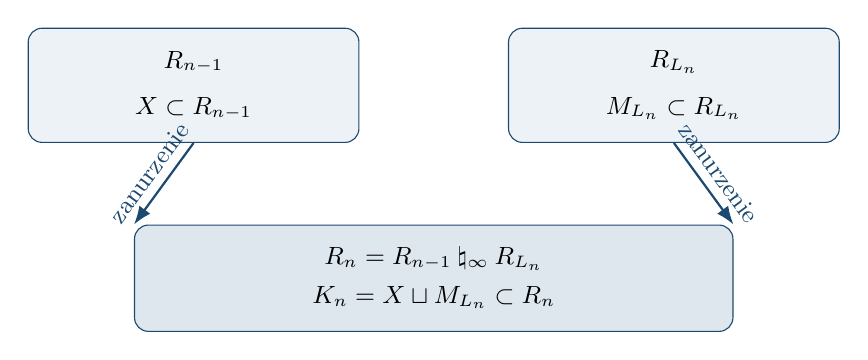
\begin{tikzpicture}[font=\small,>=Latex,
  every node/.style={align=center}]
 \node[draw=manifoldblue!80!black,rounded corners=5pt,
       fill=manifoldblue!8,minimum width=4.2cm,
       minimum height=1.45cm] (old) at (-3.05,1.35)
       {$R_{n-1}$\\[2mm]$X\subset R_{n-1}$};
 \node[draw=manifoldblue!80!black,rounded corners=5pt,
       fill=manifoldblue!8,minimum width=4.2cm,
       minimum height=1.45cm] (new) at (3.05,1.35)
       {$R_{L_n}$\\[2mm]$M_{L_n}\subset R_{L_n}$};
 \node[draw=manifoldblue!80!black,rounded corners=5pt,
       fill=manifoldblue!15,minimum width=7.6cm,
       minimum height=1.35cm] (sum) at (0,-1.1)
       {$R_n=R_{n-1}\mathbin{\natural_\infty}R_{L_n}$\\[1mm]
        $K_n=X\sqcup M_{L_n}\subset R_n$};
 \draw[->,thick,manifoldblue!80!black] (old.south)
       -- node[left,sloped,above] {zanurzenie} (sum.north west);
 \draw[->,thick,manifoldblue!80!black] (new.south)
       -- node[right,sloped,above] {zanurzenie} (sum.north east);
\end{tikzpicture}
\caption{Schemat indukcji Gompfa: oba zanurzenia
umieszczają $K_n=X\sqcup M_{L_n}$ w $R_n$.
Rysunek nie przedstawia egzotycznego końca.}
\label{fig:egzotyczne-r4-indukcja}
\end{figure}

Rysunek~\ref{fig:egzotyczne-r4-indukcja} pokazuje
rolę zwartego świadka: $K_n$ \emph{zanurza się}
w $R_n$, lecz \emph{nie zanurza się} w $R_{n-1}$.
Sama odmienność diagramów splotów $L_n$ nie
rozróżniałaby rozmaitości. Silniejsze
\href{https://doi.org/10.4310/jdg/1214439566}
{twierdzenie~1.3 Gompfa} obejmuje ponadto graniczną
rozmaitość $R_\infty$. Dla skończonych indeksów
$m,n\in\N_0$ powyższy dowód daje porządek
zorientowanych zanurzeń:
$R_m\hookrightarrow R_n$ wtedy i tylko wtedy,
gdy $m\leq n$.

\section{Małe i duże egzotyczne \texorpdfstring{$\R^4$}{R4}}
\label{sec:egzotyczne-r4-male-duze}
\index{przestrzeń euklidesowa!mała egzotyczna $\R^4$}
\index{przestrzeń euklidesowa!duża egzotyczna $\R^4$}

Egzotyczna $\R^4$ jest \emph{mała}, gdy zanurza
się gładko w standardowej $\R^4$, i \emph{duża}
w przeciwnym razie. Przy równości wymiarów
zanurzenie jest dyfeomorfizmem na otwarty
podzbiór celu. Nazwy nie dotyczą rozmiaru
metrycznego.

\begin{twierdzenie}[De Michelis--Freedman:
małe egzotyczne $\R^4$; wynik zewnętrzny]
\label{thm:egzotyczne-r4-male}
Istnieje rodzina mocy kontinuum otwartych
podzbiorów standardowej $\R^4$, z których
każdy jest homeomorficzny z $\R^4$, a każde
dwa są niedyfeomorficzne.
\end{twierdzenie}

Wynik ten pochodzi z
\href{https://doi.org/10.4310/jdg/1214447810}
{S.~De Michelisa i M.~H.~Freedmana,
\emph{Uncountably many exotic $\R^4$'s in
standard 4-space}, J.~Differential Geom. 35
(1992), 219--254}. Dowód jest osobnym głębokim
wejściem. Po usunięciu co najwyżej jednego typu
standardowego pozostaje kontinuum małych
egzotycznych $\R^4$. Każda skonstruowana wyżej
$R_n$ dla $n\geq1$ jest natomiast duża: zawiera
$X$, które nie zanurza się w standardowej $\R^4$.
Zanurzenie odwracające orientację po złożeniu
z odbiciem celu także przeczyłoby tej przeszkodzie.

\par\smallskip
{\footnotesize\noindent\emph{Dalsza lektura:}
\href{https://doi.org/10.4310/jdg/1214439566}
{R.~E.~Gompf, \emph{An infinite set of exotic $\R^4$'s}},
§1: lematy konstrukcyjne i pełne twierdzenie o rodzinie;
\href{https://doi.org/10.4310/jdg/1214447810}
{S.~De Michelis i M.~H.~Freedman,
\emph{Uncountably many exotic $\R^4$'s in standard 4-space}},
małe egzotyczne struktury.\par}


\part{Dodatki}
\appendix
\chapter{Zależności zewnętrzne i poziom samowystarczalności}
\label{app:wyniki-zewnetrzne}

W skrypcie dowód oznacza rzeczywiste
wyprowadzenie ze wskazanych wcześniejszych
faktów. Jeśli korzystamy z długiego
twierdzenia spoza tekstu, podajemy
hipotezy, miejsce użycia i źródło.
Poniższy katalog ułatwia rozpoznanie
tych punktów zależności.

\section{Wyniki wejściowe i głębokie lematy}
\label{sec:katalog-wynikow}

\begin{description}[leftmargin=2.9cm,style=nextline]
\item[Niezmienniczość obszaru.]
  Ciągła injekcja z otwartego
  $U\subset\R^n$ do $\R^n$
  ma otwarty obraz. Użyta w
  Rozdziale~\ref{ch:rozmaitosci}
  do niezależności wymiaru i
  brzegu od map.
  Źródło:
  \href{https://pi.math.cornell.edu/~hatcher/AT/AT.pdf}
  {A.\ Hatcher, \emph{Algebraic Topology},
  twierdzenie 2B.3}.
  Alternatywny dowód samej
  niezmienniczości wymiaru rozmaitości
  przez homologię lokalną jest poniżej.

\item[Twierdzenie o funkcji odwrotnej.]
  Dla $C^1$ odwzorowania między
  otwartymi podzbiorami $\R^n$
  z odwracalną pochodną w punkcie
  istnieje lokalna odwrotność $C^1$;
  dla danych $C^\infty$ jest ona
  $C^\infty$. Użyte przy mapach,
  zanurzeniach i funkcjach Morse'a.
  Źródło z dowodem:
  \href{https://www.ocw.mit.edu/courses/18-101-analysis-ii-fall-2005/d2c8fc5fe57cd59efc99caa048983d4c_lecture6.pdf}
  {V.\ Guillemin, \emph{Analysis II},
  wykład 6}.

\item[Miara Hausdorffa w przestrzeni euklidesowej.]
  Identyfikacja znormalizowanej miary Hausdorffa
  $\mathcal H^k$ na $\R^k$ z miarą Lebesgue'a,
  użyta w Rozdziale~\ref{ch:metryka-riemannowska},
  korzysta z nierówności izodiametrycznej i z twierdzenia
  Vitalego o pokryciu. Sam rachunek normalizacji oraz
  zastosowanie w mapach rozmaitości są w rozdziale,
  natomiast te dwa fakty miarowe pozostają zewnętrzne.
  Źródło:
  \href{https://www.math.cmu.edu/~gautam/sj/teaching/2022-23/720-measure/pdfs/measure.pdf}
  {G.\ Iyer, \emph{Lecture Notes on Measure Theory},
  dodatek A}.

\item[Triangulacja gładka.]
  Każda gładka rozmaitość
  drugoprzeliczalna dopuszcza
  triangulację zgodną ze
  strukturą gładką; w przypadku
  zwartym może być skończona.
  Używamy jej do przejścia od
  geometrii do skończonych
  kompleksów łańcuchowych.
  Źródło:
  \href{https://www.ams.org/bull/1935-41-08/S0002-9904-1935-06140-3/S0002-9904-1935-06140-3.pdf}
  {S.~S.\ Cairns, \emph{Triangulation of the
  Manifold of Class One}, §1--2}, oraz
  \href{https://doi.org/10.2307/1968861}
  {J.~H.~C.\ Whitehead, \emph{On $C^1$-complexes}}.
  Pełny dowód nie jest krótkim
  uzupełnieniem tego skryptu.

\item[Kohomologia Čech i singularna.]
  Każde pokrycie rozmaitości ma
  rozdrobnienie będące dobrym pokryciem.
  Dobre pokrycia tworzą więc rodzinę
  kofinalną w definicji kohomologii
  Čecha. Dla dobrego pokrycia kompleks
  Čecha oblicza kohomologię nerwu,
  a lemat o nerwie utożsamia jego
  typ homotopijny z rozmaitością.
  Dla współczynników w dyskretnej
  grupie abelowej otrzymujemy stąd
  izomorfizm kohomologii Čecha
  i singularnej. Interpretacja
  kocyklu przejść struktury
  spinowej w Rozdziale~\ref{ch:grass-spin}
  używa tego porównania;
  tam, gdzie wystarcza stopień
  pierwszy, podano też argument
  przez monodromię pętli.
  Istnienie dobrych pokryć opisują
  \href{https://doi.org/10.1007/978-1-4757-3951-0}
  {R.\ Bott i L.~W.\ Tu, \emph{Differential Forms in
  Algebraic Topology}, §5}. Wybierając użyte tam dostatecznie
  małe geodezyjnie wypukłe kule podporządkowane zadanemu pokryciu,
  otrzymujemy dobre rozdrobnienie; to daje potrzebną kofinalność.
  Pozostałe składniki porównania:
  \href{https://pi.math.cornell.edu/~hatcher/AT/AT.pdf}
  {A.\ Hatcher, \emph{Algebraic Topology},
  wniosek 4G.3 o nerwie dobrego pokrycia
  oraz §2.1 i §3.1 o kohomologii
  symplicjalnej i singularnej}.

\item[Trik Whitneya i ruchy uchwytów.]
  Niech $P^r,Q^s$ będą domkniętymi, poprzecznie
  przecinającymi się gładkimi podrozmaitościami
  $V^{r+s}$ bez brzegu; orientujemy $P$ i wiązkę
  normalną $Q$. Usunięcie punktów przecięcia $u,v$
  o przeciwnych znakach wymaga $r\geq2$, $s\geq3$
  i $r+s\geq5$. Łuki łączące $u,v$ w $P$ i $Q$
  mają wnętrzami omijać pozostałe przecięcia, a utworzony
  przez nie okrąg ma być ściągalny w $V$. Przy $r=2$
  zakładamy ponadto injektywność
  $\pi_1(V\setminus Q)\to\pi_1(V)$. Konstrukcja daje
  odpowiednio obramowany dysk Whitneya i izotopię
  usuwającą tę parę przecięć.
  Użyte w
  Rozdziałach~\ref{ch:hcobordyzm}--\ref{ch:przeszkoda-chirurgiczna}.
  Źródło warunków i konstrukcji:
  \href{https://www.math.columbia.edu/~jmorgan/Lecture_IIIA_hcobordism_Contd.pdf}
  {J.\ Morgan, \emph{The $h$-Cobordism Theorem},
  wykład IIIA}, oraz
  \href{https://webhomes.maths.ed.ac.uk/~v1ranick/surgery/hcobord.pdf}
  {J.\ Milnor, \emph{Lectures on the $h$-Cobordism Theorem},
  twierdzenie 6.6 i lematy 6.7, 6.13}.

\item[Dwie chirurgii okręgu w $S^4$.]
  Dla standardowego okręgu dwa zorientowane obramowania
  dają produktową i nietrywialną wiązkę $S^2$ nad $S^2$.
  Rozdział~\ref{ch:chirurgia-geometryczna-21} oblicza ich formy
  przecięcia; identyfikacja nietrywialnej wiązki z
  $\mathbb{CP}^2\#\overline{\mathbb{CP}^2}$ pozostaje wejściem z
  \href{https://arxiv.org/abs/1502.06834}
  {K.\ Larsona, \emph{Surgery on tori in the 4-sphere},
  dowód propozycji 4.3} oraz
  \href{https://www.mathematik.hu-berlin.de/~wendl/pub/rationalRuled.pdf}
  {C.\ Wendla, \emph{Holomorphic Curves in Low Dimensions},
  przykład 1.11 i uwaga 1.13}.
  Nie jest to zastosowanie wysokowymiarowego
  twierdzenia Walla.

\item[Torsja Whiteheada i $s$-kobordyzm.]
  Dla równoważności homotopijnej spójnych skończonych
  kompleksów CW zerowanie torsji Whiteheada jest równoważne
  prostocie tej równoważności. Wynik ten stosujemy w
  Rozdziale~\ref{ch:s-kobordyzm}; źródło:
  \href{https://webhomes.maths.ed.ac.uk/~v1ranick/papers/owsem.pdf}
  {M.\ Kreck i W.\ Lück, \emph{The Novikov Conjecture},
  twierdzenie 6.15(1)}. Drugim wejściem jest utożsamienie
  torsji uporządkowanego kompleksu Morse'a z torsją
  komórkową zgodnej gładkiej triangulacji oraz niezależność
  tej klasy od triangulacji; zob.
  \href{https://webhomes.maths.ed.ac.uk/~v1ranick/papers/milnorwh.pdf}
  {J.\ Milnor, \emph{Whitehead Torsion}, lemat 9.1
  i twierdzenie 9.3}. Po tych wejściach rozdział dowodzi,
  że dla spójnego zwartego gładkiego $h$-kobordyzmu
  $(W^m;N_-,N_+)$ o niepustych, spójnych i zamkniętych
  brzegach, $m\geq6$, zachodzi
  $\tau(W,N_-)=0$ wtedy i tylko wtedy, gdy
  $W\cong N_-\times I$ relatywnie do $N_-$;
  orientowalność nie jest założeniem.
  Przykład 6.6 Milnora oblicza osobno
  $\operatorname{Wh}(C_5)\cong\Z$ z generatorem
  $[1-t-t^{-1}]$; używamy go w
  Przykładzie~\ref{prz:Tate-C5-22}.

\item[Twierdzenia Walla.]
  Niech $(f,b):M^n\to X^n$ będzie normalnym
  odwzorowaniem stopnia jeden między spójnymi,
  zamkniętymi, gładkimi rozmaitościami, $n\geq5$,
  z charakterem orientacji $w$ na
  $\pi=\pi_1(X)$. Przeszkoda
  $\theta(f,b)\in L_n^s(\Z[\pi],w)$ znika wtedy
  i tylko wtedy, gdy $(f,b)$ jest normalnie
  kobordantne z prostą równoważnością homotopijną.
  W wersji zwartej z brzegiem odwzorowanie brzegowe
  ma być prostą równoważnością, a kobordyzm i chirurgie
  wykonuje się relatywnie do brzegu. Przypadek parzysty
  $n=2k\geq6$ daje twierdzenie 5.6 Walla, a przypadek
  nieparzysty $n=2k+1\geq5$, obejmujący wymiar pięć,
  daje twierdzenie 6.4; nie należy go mylić z nieparzystym
  twierdzeniem realizacyjnym 6.5, którego zakres zaczyna
  się w wymiarze siedem.

  Rozdział~\ref{ch:przeszkoda-chirurgiczna}
  rozpisuje rachunek przecięć i konstrukcję
  bazy hiperbolicznej nad $\Z[\pi]$,
  chirurgie poniżej środka, ciągi dokładne jąder,
  dualność oraz część ruchów formacji. Osobnymi
  wejściami pozostają przygotowanie kobordyzmu,
  bazowość i prosta dualność jego jąder,
  realizacja względnych immersji, geometryczne lematy
  Walla oraz pełna realizacja ruchów nieparzystych.

  Wersja z jedynie zwykłą równoważnością na brzegu ma
  przeszkodę $\theta^h(f,b)\in L_n^h(\Z[\pi],w)$.
  Homomorfizm zapominający prostotę
  $L_n^s\to L_n^h$ i jego związek z grupą
  Whiteheada opisuje ciąg dokładny Rothenberga z grupami
  Tate'a $\widehat H^*(\Z/2;\operatorname{Wh}(\pi))$.
  Te twierdzenia są zewnętrzne; zob.
  \href{https://www.maths.ed.ac.uk/~v1ranick/surgery/ranicki.pdf}
  {A.\ Ranicki, \emph{An Introduction to Algebraic Surgery},
  wstęp i przykład 2.16},
  \href{https://webhomes.maths.ed.ac.uk/~v1ranick/books/scm.pdf}
  {Walla, §17D}.

  Osobnym wejściem jest rozszczepienie Shanesona--Ranickiego
  $L_n^s(\Z[G\times\Z],w\oplus1)
   \cong L_n^s(\Z[G],w)\oplus L_{n-1}^h(\Z[G],w)$
  dla dodatkowego generatora zachowującego orientację.
  W przypadku $G=1$ prowadzi ono do tabeli
  $L_n^s(\Z[t,t^{-1}],1)$ w
  Sekcji~\ref{sec:L-pi1-Z-22}. Źródła:
  \href{https://webhomes.maths.ed.ac.uk/~v1ranick/papers/shan.pdf}
  {J.\ Shaneson, \emph{Wall's Surgery Obstruction Groups
  for $G\times\Z$}, twierdzenie 5.1, wariant geometryczny
  dla $G=\pi_1(K^{n-2})$, $w=w_1(K)$, $n\geq7$
  i zamkniętej gładkiej lub PL rozmaitości $K$} oraz
  \href{https://webhomes.maths.ed.ac.uk/~v1ranick/papers/splitkl.pdf}
  {A.\ Ranicki, \emph{Algebraic and Geometric Splittings
  of the K- and L-Groups of Polynomial Extensions}, §6,
  wariant algebraiczny dla dowolnej grupy}.

  Dla spójnej zamkniętej gładkiej $X^n$, $n\geq5$,
  identyfikacja $\mathcal N_{\mathrm{DIFF}}(X)\cong[X,G/O]$,
  działanie $L_{n+1}^s$ na prostym zbiorze struktur i ciąg
  chirurgii
  \[
   [\Sigma X_+,G/O]\longrightarrow
   L_{n+1}^s(\Z[\pi],w)
   \longrightarrow\mathcal S^s_{\mathrm{DIFF}}(X)
   \longrightarrow[X,G/O]\longrightarrow
   L_n^s(\Z[\pi],w)
  \]
  są kolejnymi zewnętrznymi wynikami Walla użytymi w
  Rozdziale~\ref{ch:ciag-chirurgii}. Realizacja elementów
  $L_{n+1}^s$ korzysta z twierdzenia 5.8 dla parzystego
  $n+1\geq6$ oraz z twierdzenia 6.5 dla nieparzystego
  $n+1\geq7$; przy $n=5$ używa się pierwszego z nich.
  Główne źródło:
  \href{https://webhomes.maths.ed.ac.uk/~v1ranick/books/scm.pdf}
  {C.~T.~C. Wall, \emph{Surgery on Compact
  Manifolds}, §§1--2, 5--6, 10 i 17D,
  zwłaszcza twierdzenia 1.2, 5.2, 5.6, 5.8,
  6.4--6.5, lemat 5.7 oraz wyniki 10.1--10.8}.
  Rozdziały~\ref{ch:przeszkoda-chirurgiczna}
  oraz~\ref{ch:ciag-chirurgii} rozpisują zastosowania,
  lecz nie zastępują tych wyników geometrycznych.

\item[Triangulacja powierzchni.]
  Dowód klasyfikacji zwartych powierzchni
  w Twierdzeniu~\ref{thm:classification-surfaces-24}
  korzysta z istnienia skończonej triangulacji
  topologicznej powierzchni; źródło:
  \href{https://pi.math.cornell.edu/~hatcher/Papers/TorusTrick.pdf}
  {A.\ Hatcher, \emph{The Kirby Torus Trick for Surfaces}}.

\item[Klasyfikacja Bardena w wymiarze pięć.]
  Jeśli $P,Q$ są zamkniętymi, zorientowanymi, gładkimi
  i jednospójnymi $5$-rozmaitościami, to izomorfizm
  $H_2(P;\Z)\to H_2(Q;\Z)$ zachowujący formę wiązania
  na torsji i klasę $w_2$ jest realizowany przez
  dyfeomorfizm zachowujący orientację. Jest to
  \href{https://www.sas.rochester.edu/mth/sites/doug-ravenel/otherpapers/barden.pdf}
  {D.\ Barden, \emph{Simply Connected
  Five-Manifolds}, twierdzenie 2.2}, zapisane jako
  Twierdzenie~\ref{thm:Barden-5-24}. Kanoniczna
  klasyfikacja modeli w
  Twierdzeniu~\ref{thm:barden-kanoniczna-24}
  jest twierdzeniem 2.3 tej samej pracy.
  Rozdział~\ref{ch:poincare-2-high} rekonstruuje argument,
  ale przyjmuje z zewnątrz obliczenia grup kobordyzmu
  $\Omega^{SO}_5$ i $\Omega^{Spin}_5$ Thoma--Nowikowa,
  uogólnione twierdzenie Hurewicza Whiteheada,
  reprezentowanie klas przez zanurzenia Haefligera oraz
  klasyfikację form wiązania Walla--Bardena. Dokładne
  miejsca w źródłach to Barden, §§0.3--0.4,
  twierdzenia 2.2--2.3 oraz lematy 3.1 i 4.1--4.4, a także
  \href{https://webhomes.maths.ed.ac.uk/~v1ranick/papers/kill.pdf}
  {C.~T.~C. Wall, \emph{Killing the Middle Homotopy Groups
  of Odd Dimensional Manifolds}, stwierdzenia 1--2
  i lemat 4(ii)}.

\item[Sygnatura i sfery Milnora.]
  Dla zamkniętej zorientowanej gładkiej
  $8$-rozmaitości $C$ używamy
  $\operatorname{sign}(C)=
  \langle(7p_2-p_1^2)/45,[C]\rangle$.
  Źródło:
  \href{https://webhomes.maths.ed.ac.uk/~v1ranick/papers/hirzrem.pdf}
  {F.\ Hirzebruch, \emph{The Signature Theorem},
  wzór na $L_2$}.
  Wzory charakterystyczne wiązek nad $S^4$ pochodzą z
  \href{https://sites.math.rutgers.edu/~feehan/teaching/math866/milnor7sphere.pdf}
  {J.\ Milnor, \emph{On Manifolds Homeomorphic
  to the 7-Sphere}, lemat 3}.
  Niezależność niezmiennika Eellsa--Kuipera
  $\mu\in\Q/\Z$ od spinowego wypełnienia korzysta ponadto
  z całkowitości indeksu $\widehat A$ operatora Diraca
  na zamkniętej spinowej $8$-rozmaitości. Źródłem wzoru
  i jego zastosowania jest
  \href{https://webhomes.maths.ed.ac.uk/~v1ranick/papers/eelskuip.pdf}
  {J.\ Eells i N.\ Kuiper, \emph{An Invariant for Certain
  Smooth Manifolds}, §6}. Klasyfikacja w
  Rozdziale~\ref{ch:sfery-Milnora} używa jako osobnych
  wyników zewnętrznych równości
  $\Theta_7=bP_8\cong\Z/28$ z
  \href{https://www.sas.rochester.edu/mth/sites/doug-ravenel/otherpapers/kervaire-milnor.pdf}
  {M.\ Kervaire'a i J.\ Milnora, \emph{Groups of Homotopy
  Spheres I}, §4 i §§7--8}, oraz zupełności $\mu$ dla
  zorientowanych gładkich sfer homeomorficznych z $S^7$
  z §6 pracy Eellsa--Kuipera.

\item[Holonomia i globalny rozkład de Rhama.]
  Dla koneksji Leviego-Civity twierdzenie
  Ambrose'a--Singera mówi, że algebra Liego holonomii
  ograniczonej jest rozpięta przez operatory
  $P_\gamma^{-1}R_q(u,v)P_\gamma$; obejmuje także fakt,
  że holonomia ograniczona jest grupą Liego. Wynik ten,
  użyty w Rozdziale~\ref{ch:krzywizna}, pochodzi z
  \href{https://doi.org/10.1090/S0002-9947-1953-0063739-1}
  {W.\ Ambrose'a i I.~M.\ Singera,
  \emph{A theorem on holonomy} (1953)}.
  W tym samym rozdziale udowodniono lokalną postać
  iloczynu, lecz globalny krok jest osobnym twierdzeniem:
  spójna, zupełna i jednospójna rozmaitość riemannowska
  bez brzegu, której pełna holonomia jest redukowalna,
  rozkłada się izometrycznie na czynnik euklidesowy
  i czynniki nieredukowalne, jednoznacznie z dokładnością
  do izometrii i przestawienia czynników. Źródła:
  \href{https://doi.org/10.1007/BF02564308}
  {G.\ de Rham, \emph{Sur la réductibilité d'un espace
  de Riemann} (1952)} oraz
  \href{https://doi.org/10.1215/ijm/1256059674}
  {H.\ Wu, \emph{On the de Rham decomposition theorem}
  (1964)}.

\item[Normalizacja topologiczna Cherna--Weila.]
  Rozdział~\ref{ch:chern-weil} dowodzi zamkniętości
  form Cherna--Weila i wzoru transgresji. Zewnętrznym
  wejściem pozostaje zgodność formy wyznaczonej przez
  $\det(I+i\Omega/(2\pi))$ z rzeczywistym obrazem
  topologicznej klasy Cherna, w szczególności $c_2$,
  oraz tożsamość $p_1(E)=-c_2(E\otimes_\R\C)$.
  Źródła:
  \href{https://pi.math.cornell.edu/~hatcher/VBKT/VB.pdf}
  {A.\ Hatcher, \emph{Vector Bundles and K-Theory},
  §3.1--3.2}, oraz
  \href{https://webusers.imj-prg.fr/~olivier.biquard/m2dg2022.pdf}
  {O.\ Biquard, \emph{Differential and Riemannian Geometry},
  §16.c, wzory (III.39) i (III.41)}.

\item[Analityczna teoria Hodge'a.]
  Dla laplasjanu Hodge'a na formach zwartej
  rozmaitości riemannowskiej bez brzegu
  jądro jest skończenie wymiarowe, a każda
  gładka forma prostopadła do jądra ma
  jednoznaczny gładki przeciwobraz
  prostopadły do jądra. Jest to
  Twierdzenie~\ref{thm:hodge-analytic-input},
  użyte w Rozdziale~\ref{ch:hodge-bochner}
  do istnienia rozkładu; jego konsekwencje
  algebraiczne i wzór Bochnera tam dowodzimy.
  Źródło:
  \href{https://doi.org/10.2307/1969552}
  {K.\ Kodaira, \emph{Harmonic Fields in
  Riemannian Manifolds} (1949)}.

\item[Analityczna teoria potoku Ricciego.]
  Gładki ściśle paraboliczny układ
  quasiliniowy drugiego rzędu na zwartej
  rozmaitości bez brzegu ma dla gładkich
  danych lokalnie w czasie jednoznaczne
  gładkie rozwiązanie; używamy także
  odpowiedniej wersji dla równania ciepła
  odwzorowań z metryką dziedziny zależną
  od czasu. W
  Twierdzeniu~\ref{thm:ricci-short-time}
  te fakty stosujemy po poprawce DeTurcka.
  Wyprowadzenie głównego symbolu i cofnięcie
  metryki przez dyfeomorfizmy są w rozdziale;
  same oszacowania paraboliczne są zewnętrzne.
  Źródło twierdzenia o krótkim czasie:
  \href{https://projecteuclid.org/journals/journal-of-differential-geometry/volume-17/issue-2/Three-manifolds-with-positive-Ricci-curvature/10.4310/jdg/1214436922.full}
  {R.\ S.\ Hamilton, \emph{Three-manifolds with
  positive Ricci curvature} (1982), \S\,4}.
  Źródło konstrukcji i równania cechowania:
  \href{https://projecteuclid.org/journals/journal-of-differential-geometry/volume-18/issue-1/Deforming-metrics-in-the-direction-of-their-Ricci-tensors/10.4310/jdg/1214509286.full}
  {D.\ DeTurck, \emph{Deforming Metrics in the
  Direction of Their Ricci Tensors} (1983)}.

\item[Wygładzanie rozmaitości trójwymiarowych.]
  Każda topologiczna rozmaitość trójwymiarowa dopuszcza
  zgodną strukturę gładką. Ten wynik Moise'a
  pozwala przejść od gładkiej postaci
  Twierdzenia~\ref{thm:poincare-trzy}
  do topologicznej postaci we
  Wniosku~\ref{cor:poincare-trzy-topologiczna}.
  Źródło: \href{https://msp.org/gtm/2015/19-1/gtm-v19-n1-p08-s.pdf}
  {M. Aschenbrenner, S. Friedl i H. Wilton,
  \emph{Decision Problems for 3-Manifolds and Their
  Fundamental Groups}, twierdzenie 3.1};
  \href{https://doi.org/10.2307/1969769}
  {E.~E. Moise, \emph{Affine Structures in
  3-Manifolds V} (1952)}.

\item[Miara Haara i ilorazy grup Liego.]
  Na każdej zwartej grupie Liego istnieje znormalizowana
  miara probabilistyczna niezmiennicza przy mnożeniu
  z lewej i z prawej strony. W
  Rozdziale~\ref{ch:geometria-kleina} służy ona do
  uśrednienia metryki względem zwartego stabilizatora.
  Źródło:
  \href{https://doi.org/10.2307/1968346}
  {A.\ Haar, \emph{Der Massbegriff in der Theorie der
  kontinuierlichen Gruppen} (1933)}.
  Dla domkniętej podgrupy $H$ skończenie wymiarowej
  grupy Liego $G$ istnienie gładkiej struktury na
  $G/H$ i submersyjność rzutowania są wejściem
  zewnętrznym w
  Twierdzeniu~\ref{thm:klein-iloraz-liego}.
  Dowód identyfikacji orbit z ilorazami oraz
  konkretne przykłady są w
  Rozdziale~\ref{ch:geometria-kleina}.
  Źródło: J.\ M.\ Lee, \emph{Introduction to Smooth
  Manifolds}, rozdziały~20--21.

\item[Potok Ricciego z chirurgią i wygaśnięcie.]
  Dla dowolnej gładkiej metryki na zamkniętej
  zorientowanej $3$-rozmaitości kontrolę osobliwości
  i kontynuację potoku przez chirurgię dostarczają
  wyniki Perelmana. Używana wersja twierdzenia o
  wygaśnięciu zakłada, że $\pi_1(M)$ jest wolnym
  iloczynem skończenie wielu grup skończonych i kopii
  $\Z$; równoważnie, w rozkładzie pierwszym nie ma
  składników asferycznych. Wówczas potok z chirurgią
  wygasa w skończonym czasie.
  W Rozdziale~\ref{ch:poincare-trzy} te twierdzenia
  oraz topologiczny opis odrzucanych składników
  są jawnymi wejściami; własne rachunki i wnioski
  nie zastępują ich dowodów. Źródła:
  \href{https://arxiv.org/pdf/math/0211159}
  {G.\ Perelman, \emph{The entropy formula for the Ricci flow} (2002)},
  \href{https://arxiv.org/pdf/math/0303109}
  {\emph{Ricci flow with surgery on three-manifolds} (2003)},
  \href{https://arxiv.org/pdf/math/0307245}
  {\emph{Finite extinction time} (2003)};
  szczegółowe opracowanie:
  \href{https://www.claymath.org/wp-content/uploads/2022/03/Ricci-pdf.pdf}
  {J.\ Morgan i G.\ Tian, \emph{Ricci Flow and the Poincaré Conjecture}}.

\item[Geometryzacja rozmaitości trójwymiarowych.]
  Rozkład pierwszy, cięcie wzdłuż istotnych torusów
  i twierdzenie geometryzacyjne dla zamkniętych
  orientowalnych $3$-rozmaitości są wynikami zewnętrznymi
  w Rozdziale~\ref{ch:geometrizacja-thurstona}.
  Opis ośmiu maksymalnych geometrii modelowych także
  korzysta z klasyfikacji zewnętrznej; przykłady i rachunki
  w rozdziale ilustrują modele, lecz jej nie dowodzą.
  Źródła:
  \href{https://library.slmath.org/nonmsri/gt3m/PDF/Thurston-gt3m.pdf}
  {W.\ Thurston, \emph{The Geometry and Topology of Three-Manifolds}},
  \href{https://sschleimer.warwick.ac.uk/Teach/2021_3MFDS/References/1983the_geometries_of_three-manifolds.pdf}
  {P.\ Scott, \emph{The Geometries of 3-Manifolds} (1983)}
  oraz \href{https://www.claymath.org/wp-content/uploads/2022/03/Geom.pdf}
  {J.\ Morgan i G.\ Tian, \emph{The Geometrization Conjecture}}.

\item[Topologiczna dualność i wygładzanie PL w wymiarze cztery.]
  W Rozdziale~\ref{ch:freedman-formy} formę przecięcia
  zamkniętej zorientowanej rozmaitości TOP opisujemy przez topologiczną
  dualność Poincarégo. Używamy także wyniku, że
  struktura PL w wymiarze cztery dopuszcza zgodne
  wygładzenie. Rachunki macierzy uchwytów i formy $E_8$
  są w rozdziale; te dwa fakty kategorialne pozostają
  wejściami zewnętrznymi. Źródło:
  \href{https://archive.mpim-bonn.mpg.de/4789/2/FreedmanQuinn-TopologyOf4Manifolds-Reformatted2013.pdf}
  {M.\ H.\ Freedman i F.\ Quinn, \emph{Topology of
  4-Manifolds}, \S\,8.7 i \S\,10.2}.

\item[Zanurzanie dysków i uchwyty Cassona.]
  W Rozdziale~\ref{ch:uchwyty-cassona} dowodzimy
  własności skończonych pięter, ale przejście do
  parami rozłącznych lokalnie płaskich dysków jest
  wejściem zewnętrznym. Użyta wersja dotyczy zwartej,
  spójnej, zorientowanej gładkiej $4$-rozmaitości
  z brzegiem i właściwych immersji obramowanych dysków
  o parami rozłącznie zanurzonych brzegach z kołnierzami.
  Zakłada obramowane immersyjne sfery $B_j$ z
  $\lambda(A_i,B_j)=\delta_{ij}$,
  $\lambda(B_i,B_j)=0$ i $\mu(B_j)=0$ nad
  $\Z[\pi_1(M)]$ oraz grupę podstawową wielostopniowo
  skończoną lub cykliczną. Konkluzja daje dyski
  topologicznie zanurzone z zachowanymi obramowanymi
  brzegami i geometrycznie dualnymi sferami:
  Twierdzenie~\ref{thm:casson-disk-embedding},
  \href{https://archive.mpim-bonn.mpg.de/4789/2/FreedmanQuinn-TopologyOf4Manifolds-Reformatted2013.pdf}
  {Freedman--Quinn, \emph{Topology of 4-Manifolds},
  Twierdzenie 5.2}. Konstrukcję geometrycznie
  dualnych sfer w konkluzji uzupełnia
  \href{https://arxiv.org/pdf/2006.05209}
  {M.\ Powell, A.\ Ray i P.\ Teichner,
  \emph{The 4-dimensional disc embedding theorem
  and dual spheres}, Twierdzenie A}; w pierwotnym
  dowodzie Freedmana--Quinna brakowało tego kroku.
  Standardowość topologiczna
  uchwytu Cassona jako pary to osobne wejście:
  Twierdzenie~\ref{thm:casson-homeomorphism},
  \href{https://www.maths.gla.ac.uk/~mpowell/1982_The%20topology%20of%20four-dimensional%20manifolds.pdf}
  {Freedman, \emph{The topology of four-dimensional
  manifolds} (1982), Twierdzenie 1.1}.

\item[Klasyfikacja Freedmana i niezmiennik Kirby'ego--Siebenmanna.]
  Twierdzenie~\ref{thm:freedman-classification}
  o zamkniętych zorientowanych jednospójnych
  rozmaitościach TOP, warunek
  $\operatorname{ks}\equiv\sigma/8\pmod2$ dla
  form parzystych oraz
  dokładne kryterium stabilnego wygładzenia
  $\operatorname{ks}(X)=0\Longleftrightarrow
  X\times\R$ jest wygładzalna
  są wejściami zewnętrznymi w
  Rozdziale~\ref{ch:freedman-klasyfikacja}.
  Kryterium to nie orzeka samo o wygładzalności $X$.
  Źródła:
  \href{https://archive.mpim-bonn.mpg.de/4789/2/FreedmanQuinn-TopologyOf4Manifolds-Reformatted2013.pdf}
  {Freedman--Quinn, \emph{Topology of 4-Manifolds},
  \S\,8.7--8.8 i \S\,10.1--10.2} oraz
  \href{https://www.maths.gla.ac.uk/~mpowell/1982_The%20topology%20of%20four-dimensional%20manifolds.pdf}
  {Freedman, \emph{The topology of four-dimensional
  manifolds} (1982), Twierdzenie 1.5}.

\item[Twierdzenie Donaldsona i analiza równań ASD.]
  Diagonalizacja określonej całkowitej formy przecięcia
  gładkiej, zamkniętej, jednospójnej $4$-rozmaitości
  jest zewnętrznym Twierdzeniem~\ref{thm:donaldson-diagonalizacja}.
  Rachunek energii w Rozdziale~\ref{ch:donaldson} jest własny,
  lecz zwartość przestrzeni moduli, analiza rozwiązań
  redukowalnych i koncentracji krzywizny nie są tu dowiedzione.
  Źródło:
  \href{https://doi.org/10.4310/jdg/1214437665}
  {S.~K.~Donaldson, \emph{An application of gauge theory
  to four-dimensional topology}, J.~Differential Geom. 18
  (1983), twierdzenie A}.

\item[Twierdzenie Rokhlina.]
  Podzielność sygnatury zamkniętej gładkiej
  spinowej $4$-rozmaitości przez $16$, użyta do
  porównania form $E_8$ i $E_8\oplus E_8$ w
  Rozdziale~\ref{ch:donaldson}, jest wynikiem
  zewnętrznym. Zob.
  \href{https://arxiv.org/pdf/2011.12418}
  {M.~R.~Klug, \emph{A relative version of Rochlin's
  theorem}, wprowadzenie}.

\item[Egzotyczne struktury gładkie na $\R^4$.]
  Istnienie początkowej zwartej przeszkody, realizacja
  śladu topologicznie plastrowalnego splotu oraz
  lemat wytwarzający następną przeszkodę są zewnętrznymi
  Twierdzeniami~\ref{thm:egzotyczne-r4-X},
  \ref{thm:egzotyczne-r4-slad} i
  \ref{thm:egzotyczne-r4-lemat}. Indukcja i rozróżnienie
  typów gładkich są rozpisane w
  Rozdziale~\ref{ch:egzotyczne-r4}.
  Źródło:
  \href{https://doi.org/10.4310/jdg/1214439566}
  {R.~E.~Gompf, \emph{An infinite set of exotic
  $\R^4$'s}, J.~Differential Geom. 21 (1985),
  lematy 1.1--1.2 i twierdzenie 1.3}.
  Dowód realizacji śladu splotu korzysta także z
  zewnętrznych twierdzeń Quinna o wygładzaniu
  niezwartych dopełnień w wymiarze cztery i o stabilnych
  homeomorfizmach; zob.
  \href{https://www.maths.gla.ac.uk/~mpowell/1982_Ends%20of%20maps%20III.pdf}
  {F.\ Quinn, \emph{Ends of maps, III: dimensions 4 and 5}
  (1982)}.
  Istnienie kontinuum małych egzotycznych $\R^4$
  w Twierdzeniu~\ref{thm:egzotyczne-r4-male}
  jest osobnym wynikiem zewnętrznym:
  \href{https://doi.org/10.4310/jdg/1214447810}
  {S.~De Michelis i M.~H.~Freedman,
  \emph{Uncountably many exotic $\R^4$'s in
  standard 4-space}, J.~Differential Geom. 35
  (1992), 219--254}.
\end{description}

\chapter{Rachunki uzupełniające}
\label{app:homologia-singularna-euler}

\section{Wybrany dowód: wymiar z homologii lokalnej}
\label{sec:local-dimension-appendix}

W Rozdziale~\ref{ch:rozmaitosci}
wyprowadziliśmy jednoznaczność
wymiaru z twierdzenia Brouwera.
Po wprowadzeniu homologii
można otrzymać inny dowód,
bez zakładania samej
niezmienniczości obszaru.

\begin{stwierdzenie}[Homologiczna niezmienniczość
wymiaru rozmaitości]
\label{prop:dimension-local-homology}
Jeżeli niepuste rozmaitości
topologiczne bez brzegu
$M^n,N^m$ są homeomorficzne,
to $n=m$.
\end{stwierdzenie}
\begin{proof}
Niech $h:M\to N$ będzie ustalonym homeomorfizmem.
Dla $p\in M$ wybieramy otoczenie współrzędnościowe
$U\cong\R^n$, w którym $p$ odpowiada zeru. Przez
wycinanie i długi ciąg
pary mamy
\[
 H_i(M,M\setminus\{p\};\Z)
 \cong H_i(\R^n,\R^n\setminus\{0\};\Z)
 \cong\widetilde H_{i-1}(S^{n-1};\Z).
\]
Drugi izomorfizm wynika z
ściągalności $\R^n$
i radialnego cofnięcia
$\R^n\setminus\{0\}$
na $S^{n-1}$.
Dla $n\geq1$ grupa
po lewej jest $\Z$
dokładnie w stopniu $i=n$
i zerowa w pozostałych
stopniach. Dla $n=0$
lokalna grupa $H_0$
jest $\Z$, co daje
ten sam sposób odczytu.
Homeomorfizm par
$(M,M\setminus\{p\})$
i $(N,N\setminus\{h(p)\})$
zachowuje wszystkie
grupy lokalne, zatem
stopień ich jedynej
niezerowej grupy jest
taki sam: $n=m$.
\end{proof}


\section{Homologia singularna i charakterystyka Eulera}
\index{homologia singularna@Homologia singularna!obliczenia}
\index{charakterystyka Eulera@Charakterystyka Eulera!obliczenia}

Homologia singularna, zdefiniowana w~\ref{def:homologia-singularna},
jest dostępna dla każdej przestrzeni topologicznej, ale jej grupy
łańcuchów są zwykle nieskończenie generowane. Nawet punkt ma po jednym
singularnym sympleksie stałym w każdym wymiarze. Dlatego nie można
otrzymać charakterystyki Eulera przez naprzemienne dodawanie liczb
\emph{wszystkich} singularnych sympleksów. Gdy przestrzeń ma skończony
model komórkowy, Twierdzenie~\ref{thm:komorkowa-singularna} zastępuje
ten duży kompleks skończonym kompleksem o tych samych homologiach.
Poniżej rozpisujemy wynikające stąd rachunki, przydatne zwłaszcza
przy rozkładach powierzchni i dołączaniu uchwytów.

\section{Dwa sposoby obliczania tej samej liczby}
\label{sec:app-euler-dwa-rachunki}

Niech $X$ będzie skończonym kompleksem CW. Oznaczmy przez $c_k(X)$
liczbę jego $k$-komórek, a przez
$b_k(X)=\dim_{\Q}H_k(X;\Q)$ jego $k$-tą liczbę Betti'ego.
Homologie po prawej stronie są \emph{singularne}; porównanie
z homologią komórkową pozwala jednak policzyć je z komórek.

\begin{stwierdzenie}[Wzór Eulera dla skończonego CW]
\label{prop:app-euler-cw}
Dla skończonego kompleksu CW $X$ zachodzi
\begin{equation}\label{eq:app-euler-cw}
 \chi(X):=\sum_{k\geq0}(-1)^k c_k(X)
 =\sum_{k\geq0}(-1)^k b_k(X).
\end{equation}
W szczególności suma po komórkach nie zależy od wybranego skończonego
rozkładu CW przestrzeni $X$.
\end{stwierdzenie}
\begin{proof}
Z Uwagi~\ref{rem:homologia-wspolczynniki-przestrzeni} kompleks
komórkowy $C_k^{\mathrm{CW}}(X;\Q)$ ma dokładnie $c_k(X)$ generatorów
nad $\Q$, a jego homologia jest $H_k(X;\Q)$ na mocy
Twierdzenia~\ref{thm:komorkowa-singularna}. Kompleks jest skończony,
więc możemy zastosować Twierdzenie~\ref{thm:euler-homologia}:
naprzemienna suma wymiarów grup łańcuchów równa się naprzemiennej
sumie wymiarów ich homologii. To dokładnie~\eqref{eq:app-euler-cw}.
Jeśli wybierzemy drugi skończony rozkład CW tej samej przestrzeni,
obie sumy komórkowe są równe tej samej sumie liczb Betti'ego.
\end{proof}

Rachunek nad $\Q$ odrzuca torsję: na przykład grupa $\Z/2\Z$
wnosi zero do rangi homologii całkowitej. Można też liczyć nad dowolnym
ciałem $\mathbb F$. Wtedy ta sama liczba komórek daje
\begin{equation}\label{eq:app-euler-cialo}
 \chi(X)=\sum_k(-1)^k\dim_{\mathbb F}H_k(X;\mathbb F).
\end{equation}
Poszczególne wymiary mogą zależeć od charakterystyki ciała,
jak dla $\mathbb{RP}^2$ w Przykładzie~\ref{prz:zmiana-wspolczynnikow-rp2-torus},
lecz ich naprzemienna suma nie zależy.
Jeśli ponadto $X=M^n$ jest zamkniętą zorientowaną
rozmaitością, dualność Poincarégo z
Wniosku~\ref{cor:pd-parowanie-16} daje
$b_k(M)=b_{n-k}(M)$. Dla nieparzystego $n$ wyrazy
w naprzemiennej sumie parują się z przeciwnymi znakami,
więc $\chi(M)=0$.

\section{Pary, dołączanie komórek i sklejanie}
\label{sec:app-euler-sklejanie}

Wzór na charakterystykę względną mierzy, ile komórek dodajemy do
już zbudowanej przestrzeni. W filtracji uchwytowej odpowiednikiem
nowej komórki jest rdzeń uchwytu.

\begin{stwierdzenie}[Charakterystyka Eulera pary CW]
\label{prop:app-euler-wzgledna}
Niech $A\subseteq X$ będzie podkompleksem skończonego kompleksu CW.
Wtedy homologie względne są skończenie wymiarowe nad $\Q$ i
\begin{equation}\label{eq:app-euler-wzgledna}
 \sum_k(-1)^k\dim_{\Q}H_k(X,A;\Q)
 =\chi(X)-\chi(A).
\end{equation}
Jeśli $X$ powstaje z $A$ przez dołączenie jednej $q$-komórki,
to $\chi(X)=\chi(A)+(-1)^q$.
\end{stwierdzenie}
\begin{proof}
Długi ciąg homologii pary $(X,A)$ nad $\Q$ z
Sekcji~\ref{sec:homologia-wzgledna} jest dokładny.
Grupy $H_k(X;\Q)$ i $H_k(A;\Q)$ są skończenie wymiarowe i znikają
ponad wymiarem $X$ na mocy Twierdzenia~\ref{thm:komorkowa-singularna}.
Dokładność pokazuje, że grupy względne także są skończenie
wymiarowe i znikają w dostatecznie wysokich stopniach.
W skończonym ciągu dokładnym przestrzeni liniowych naprzemienna suma
wymiarów wynosi zero: wymiar każdego wyrazu jest sumą wymiarów
obrazu strzałki wchodzącej i wychodzącej, a te składniki znoszą się
parami. Wyrazy długiego ciągu występują w porządku
$H_k(A)\to H_k(X)\to H_k(X,A)\to H_{k-1}(A)$;
po zsumowaniu dostajemy
$0=\chi(A)-\chi(X)+\sum_k(-1)^k\dim_{\Q}H_k(X,A;\Q)$.
Zatem
$\chi(X)=\chi(A)+\sum_k(-1)^k\dim_{\Q}H_k(X,A;\Q)$,
co jest tezą. Jeśli dodajemy jedną $q$-komórkę, to liczby komórek
$X$ i $A$ różnią się tylko o~$1$ w stopniu $q$.
\end{proof}

\begin{wniosek}[Liczba uchwytów i charakterystyka Eulera]
\label{cor:app-euler-uchwyty}
Niech zwarty kobordyzm $W$ od $N_-$ ma skończony rozkład uchwytowy
z $u_k$ uchwytami indeksu $k$, a $N_-$ niech ma skończony model CW.
Wówczas
\[
 \chi(W)-\chi(N_-)=\sum_k(-1)^k u_k.
\]
\end{wniosek}
\begin{proof}
Względny rozkład uchwytowy daje model CW pary
$(W,N_-)$ z jedną względną $k$-komórką na każdy
uchwyt indeksu $k$. Po dołączeniu tych skończenie wielu
komórek do skończonego modelu CW przestrzeni $N_-$
otrzymujemy skończony model CW przestrzeni $W$;
dlatego $\chi(N_-)$ i $\chi(W)$ z
równania~\eqref{eq:app-euler-cw} są określone.
Twierdzenie~\ref{thm:kompleks-uchwytow-18} daje skończony kompleks
całkowity; po tensorowaniu z $\Q$ zgodnie z
Twierdzeniem~\ref{thm:homologia-char-zero} oblicza on
$H_*(W,N_-;\Q)$ i ma przestrzeń wymiaru $u_k$ w stopniu $k$.
Twierdzenie~\ref{thm:euler-homologia}
utożsamia naprzemienną sumę tych wymiarów z naprzemienną sumą
wymiarów homologii względnych. Długi ciąg pary, dokładnie jak
w dowodzie Stwierdzenia~\ref{prop:app-euler-wzgledna}, utożsamia
tę ostatnią sumę z $\chi(W)-\chi(N_-)$.
\end{proof}

\begin{stwierdzenie}[Addytywność przy sklejaniu podkompleksów]
\label{prop:app-euler-addytywnosc}
Jeśli $X=A\cup B$, gdzie $A$ i $B$ są podkompleksami skończonego
kompleksu CW $X$, to
\begin{equation}\label{eq:app-euler-sklejanie}
 \chi(X)=\chi(A)+\chi(B)-\chi(A\cap B).
\end{equation}
\end{stwierdzenie}
\begin{proof}
Każda otwarta komórka $X$ należy do $A$, do $B$ albo do obu.
W każdym wymiarze zwykłe liczenie zbiorów komórek daje
$c_k(X)=c_k(A)+c_k(B)-c_k(A\cap B)$.
Mnożymy tę równość przez $(-1)^k$ i sumujemy po skończonej liczbie
wymiarów. Wzór~\eqref{eq:app-euler-cw} zapewnia, że wynik jest też
rachunkiem z homologii singularnej.
\end{proof}

\begin{przyklad}[Sfera z dwóch dysków]
Rozłóżmy $S^2$ na dwa domknięte dyski ze wspólnym brzegiem $S^1$
i wybierzmy zgodne, skończone struktury CW, dla których dyski oraz
okrąg są podkompleksami. Dysk ma jedną $0$-komórkę, jedną
$1$-komórkę na brzegu i jedną $2$-komórkę, więc $\chi(D^2)=1$;
okrąg ma po jednej komórce w wymiarach $0$ i $1$, więc
$\chi(S^1)=0$. Wzór~\eqref{eq:app-euler-sklejanie} daje
$\chi(S^2)=1+1-0=2$. Zgadza się to z obliczeniem
$H_0(S^2;\Q)=H_2(S^2;\Q)=\Q$ i $H_1(S^2;\Q)=0$
z Twierdzenia~\ref{thm:homologia-sfer}.
\end{przyklad}

\section{Wielokąty powierzchni: brzegi i cecha Eulera}
\label{sec:app-euler-powierzchnie}

Rozważmy najpierw powierzchnię $\Sigma_g$ otrzymaną ze standardowego
wielokąta o słowie brzegowym
\[
 a_1b_1a_1^{-1}b_1^{-1}\cdots
 a_gb_ga_g^{-1}b_g^{-1},\qquad g\geq1.
\]
Po sklejeniu wszystkie wierzchołki dają jeden wierzchołek,
pary boków dają $2g$ krawędzi, a wnętrze wielokąta jedną
$2$-komórkę. Obliczmy brzegi, zamiast zatrzymywać się na samym
liczeniu komórek. Każda $1$-komórka jest pętlą, więc
$\partial_1=0$. Współczynnik $\partial_2$ przy danej
$1$-komórce jest sumą jej przebiegów w słowie brzegowym ze znakami
orientacji, zgodnie z konstrukcją w~\ref{sec:homologia-komorkowa}.
Każda litera pojawia się tu raz dodatnio i raz ujemnie, zatem
$\partial_2=0$. Kompleks i jego homologie mają więc postać
\[
 0\longrightarrow\Z\xrightarrow{\;0\;}\Z^{2g}
 \xrightarrow{\;0\;}\Z\longrightarrow0,
 \qquad
 H_2(\Sigma_g;\Z)=\Z,\quad
 H_1(\Sigma_g;\Z)=\Z^{2g},\quad
 H_0(\Sigma_g;\Z)=\Z.
\]
Stąd $\chi(\Sigma_g)=1-2g+1=2-2g$.
Dla $g=0$ analogiczny model sfery ma jedną $0$-komórkę
i jedną $2$-komórkę; ten sam wzór daje $\chi(S^2)=2$.

Model nieorientowalny $N_h$ otrzymujemy z wielokąta o słowie
$c_1c_1\cdots c_hc_h$, gdzie $h\geq1$.
Znów jest jeden wierzchołek i jedna $2$-komórka, lecz tym razem
jest $h$ krawędzi, a każdą z nich brzeg obiega dwa razy w tym samym
kierunku. Dla standardowej bazy $e_1,\ldots,e_h$ mamy zatem
\[
 0\longrightarrow\Z\xrightarrow{\;\partial_2\;}\Z^h
 \xrightarrow{\;0\;}\Z\longrightarrow0,
 \qquad \partial_2(1)=2(e_1+\cdots+e_h).
\]
Wektor $v=e_1+\cdots+e_h$ można uzupełnić do bazy
$(v,e_2,\ldots,e_h)$ grupy $\Z^h$, ponieważ
$e_1=v-e_2-\cdots-e_h$.
Dlatego $\partial_2$ jest injekcją i
\[
 H_2(N_h;\Z)=0,\qquad
 H_1(N_h;\Z)\cong\Z^{h-1}\oplus\Z/2\Z,\qquad
 H_0(N_h;\Z)=\Z.
\]
Cecha Eulera wynosi $\chi(N_h)=1-h+1=2-h$;
po przejściu do współczynników $\Q$ tę samą wartość daje
$1-(h-1)$. Przypadek $h=1$ odtwarza rachunek dla
$\mathbb{RP}^2$ z Przykładu~\ref{prz:homologia-rp2}.
Te obliczenia dotyczą wskazanych modeli wielokątowych; pełne
twierdzenie o klasyfikacji wszystkich zwartych powierzchni
jest osobnym wynikiem używanym w Rozdziale~\ref{ch:poincare-2-high}.

\chapter{Ważne grupy macierzowe i ich algebry Liego}
\label{app:grupy-algebry-macierzowe}

\index{grupa Liego!macierzowa}
\index{algebra Liego!macierzowa}
\index{komutator macierzy}
\index{nawias Liego}

W dodatku zbieramy najważniejsze klasyczne grupy macierzowe oraz
odpowiadające im algebry Liego. Pozwala to uniknąć oddzielnego
omawiania tych samych obiektów w dwóch miejscach.

Jeśli $G$ jest macierzową grupą Liego, jej algebra Liego jest
przestrzenią styczną w elemencie neutralnym:
\[
\mathfrak g=T_IG.
\]
Dla grup macierzowych można ją traktować jako odpowiednią przestrzeń
macierzy z nawiasem
\[
[X,Y]:=XY-YX.
\]
W szczególności
\[
\dim G=\dim\mathfrak g.
\]

W przypadku grup zespolonych będziemy zaznaczać, czy wymiar liczony
jest nad $\mathbb C$, czy nad $\mathbb R$. Jeśli $G$ jest zespoloną
grupą Liego, to
\[
\dim_{\mathbb R}G
=
2\dim_{\mathbb C}G.
\]
Dalej $n\geq1$, $\mathbb K\in\{\R,\C\}$ oraz
$\mathbb K_*=\mathbb K\setminus\{0\}$.
Wymiar ilorazu przez domkniętą podgrupę liczymy
według Twierdzenia~\ref{thm:klein-iloraz-liego}.


% ============================================================
% GL
% ============================================================

\section{Ogólna grupa liniowa i algebra
\texorpdfstring{$\mathfrak{gl}(n,\mathbb K)$}{gl(n,K)}}
\label{sec:app-grupa-gl}

\index{grupa Liego!GL@$GL(n,\mathbb K)$}
\index{ogólna grupa liniowa}
\index{algebra Liego!gl@$\mathfrak{gl}(n,\mathbb K)$, ogólna liniowa}

Niech $\mathbb K=\mathbb R$ lub $\mathbb C$.

\begin{definicja}
\emph{Ogólną grupą liniową} nazywamy
\[
GL(n,\mathbb K)
=
\{A\in M_n(\mathbb K):\det A\neq0\}.
\]
Jej algebra Liego jest równa
\[
\mathfrak{gl}(n,\mathbb K)
=
M_n(\mathbb K).
\]
\end{definicja}

Ponieważ $GL(n,\mathbb K)$ jest otwartym podzbiorem
$M_n(\mathbb K)$, otrzymujemy
\[
\dim_{\mathbb R}GL(n,\mathbb R)
=
\dim_{\mathbb R}\mathfrak{gl}(n,\mathbb R)
=
n^2,
\]
natomiast
\[
\dim_{\mathbb C}GL(n,\mathbb C)
=
\dim_{\mathbb C}\mathfrak{gl}(n,\mathbb C)
=
n^2.
\]
Jako rzeczywiste rozmaitości
\[
\dim_{\mathbb R}GL(n,\mathbb C)=2n^2.
\]


% ============================================================
% SL
% ============================================================

\section{Specjalna grupa liniowa i algebra
\texorpdfstring{$\mathfrak{sl}(n,\mathbb K)$}{sl(n,K)}}

\index{grupa Liego!SL@$SL(n,\mathbb K)$}
\index{specjalna grupa liniowa}
\index{algebra Liego!sl@$\mathfrak{sl}(n,\mathbb K)$, specjalna liniowa}
\index{ślad macierzy}

\begin{definicja}
\emph{Specjalną grupą liniową} nazywamy
\[
SL(n,\mathbb K)
=
\{A\in GL(n,\mathbb K):\det A=1\}.
\]
Jej algebra Liego jest równa
\[
\mathfrak{sl}(n,\mathbb K)
=
\{X\in M_n(\mathbb K):\operatorname{tr}X=0\}.
\]
\end{definicja}

Warunek
\[
\operatorname{tr}X=0
\]
jest jednym niezależnym warunkiem liniowym. Dlatego
\[
\dim_{\mathbb R}SL(n,\mathbb R)
=
\dim_{\mathbb R}\mathfrak{sl}(n,\mathbb R)
=
n^2-1,
\]
a w przypadku zespolonym
\[
\dim_{\mathbb C}SL(n,\mathbb C)
=
\dim_{\mathbb C}\mathfrak{sl}(n,\mathbb C)
=
n^2-1.
\]
W szczególności
\[
\dim_{\mathbb R}SL(n,\mathbb C)=2(n^2-1).
\]


% ============================================================
% O i SO
% ============================================================

\section{Grupy ortogonalne i algebra
\texorpdfstring{$\mathfrak{so}(n)$}{so(n)}}
\label{sec:app-grupa-o}

\index{grupa Liego!O@$O(n)$}
\index{grupa Liego!SO@$SO(n)$}
\index{grupa ortogonalna}
\index{specjalna grupa ortogonalna}
\index{algebra Liego!so@$\mathfrak{so}(n)$, ortogonalna}
\index{macierz!antysymetryczna}

\begin{definicja}
\emph{Grupą ortogonalną} nazywamy
\[
O(n)
=
\{A\in GL(n,\mathbb R):A^TA=I\},
\]
natomiast \emph{specjalną grupą ortogonalną}
\[
SO(n)
=
\{A\in O(n):\det A=1\}.
\]
\end{definicja}

Obie grupy mają tę samą algebrę Liego:
\[
\operatorname{Lie}(O(n))
=
\operatorname{Lie}(SO(n))
=
\mathfrak{so}(n),
\]
gdzie
\[
\mathfrak{so}(n)
=
\{X\in M_n(\mathbb R):X^T=-X\}.
\]

Macierz antysymetryczna ma zerową przekątną, a dla $i<j$
współczynnik $x_{ij}$ może być wybrany dowolnie, po czym
\[
x_{ji}=-x_{ij}.
\]
Liczba niezależnych parametrów wynosi więc
\[
\binom n2=\frac{n(n-1)}2.
\]
Stąd
\[
\boxed{
\dim O(n)
=
\dim SO(n)
=
\dim\mathfrak{so}(n)
=
\frac{n(n-1)}2.
}
\]

Grupa $O(n)$ ma dwie składowe spójności, odpowiadające warunkom
$\det A=1$ i $\det A=-1$. Algebra Liego nie wykrywa tej różnicy,
ponieważ opisuje lokalną strukturę grupy jedynie w otoczeniu
elementu neutralnego.


% ============================================================
% SO(n,C)
% ============================================================

\section{Zespolona grupa ortogonalna}

\index{grupa Liego!SOC@$SO(n,\mathbb C)$}
\index{algebra Liego!soC@$\mathfrak{so}(n,\mathbb C)$, ortogonalna zespolona}

Definiujemy
\[
SO(n,\mathbb C)
=
\{A\in GL(n,\mathbb C):
A^TA=I,\ \det A=1\}.
\]
Jej algebra Liego ma postać
\[
\mathfrak{so}(n,\mathbb C)
=
\{X\in M_n(\mathbb C):X^T=-X\}.
\]

Stąd
\[
\boxed{
\dim_{\mathbb C}SO(n,\mathbb C)
=
\dim_{\mathbb C}\mathfrak{so}(n,\mathbb C)
=
\frac{n(n-1)}2.
}
\]
Jako rzeczywista grupa Liego ma ona wymiar
\[
n(n-1).
\]


% ============================================================
% U i SU
% ============================================================

\section{Grupy unitarne i ich algebry Liego}
\label{sec:app-grupa-u}

\index{grupa Liego!U@$U(n)$}
\index{grupa Liego!SU@$SU(n)$}
\index{grupa unitarna}
\index{specjalna grupa unitarna}
\index{algebra Liego!u@$\mathfrak u(n)$, unitarna}
\index{algebra Liego!su@$\mathfrak{su}(n)$, specjalna unitarna}
\index{macierz!antyhermitowska}

Przez
\[
A^*:=\overline A^{\,T}
\]
oznaczamy sprzężenie hermitowskie macierzy.

\begin{definicja}
\emph{Grupą unitarną} nazywamy
\[
U(n)
=
\{A\in GL(n,\mathbb C):A^*A=I\},
\]
natomiast \emph{specjalną grupą unitarną}
\[
SU(n)
=
\{A\in U(n):\det A=1\}.
\]
\end{definicja}

Ich algebry Liego są odpowiednio równe
\[
\mathfrak u(n)
=
\{X\in M_n(\mathbb C):X^*=-X\}
\]
oraz
\[
\mathfrak{su}(n)
=
\{X\in M_n(\mathbb C):
X^*=-X,\ \operatorname{tr}X=0\}.
\]

Macierz antyhermitowska ma czysto urojone elementy diagonalne,
co daje $n$ parametrów rzeczywistych. Dla każdej pary $i<j$
element $x_{ij}\in\mathbb C$ jest dowolny, a
\[
x_{ji}=-\overline{x_{ij}}.
\]
Każda taka para daje dwa parametry rzeczywiste. Zatem
\[
n+2\binom n2=n^2.
\]
Otrzymujemy
\[
\boxed{
\dim_{\mathbb R}U(n)
=
\dim_{\mathbb R}\mathfrak u(n)
=
n^2.
}
\]

Warunek $\operatorname{tr}X=0$ usuwa jeden rzeczywisty parametr,
dlatego
\[
\boxed{
\dim_{\mathbb R}SU(n)
=
\dim_{\mathbb R}\mathfrak{su}(n)
=
n^2-1.
}
\]

W szczególności
\[
\dim SU(2)=3,
\qquad
\dim SU(3)=8.
\]

Algebry $\mathfrak u(n)$ i $\mathfrak{su}(n)$ są naturalnie
rzeczywistymi algebrami Liego, mimo że składają się z macierzy
zespolonych.


% ============================================================
% Sp(2n,R)
% ============================================================

\section{Rzeczywista grupa symplektyczna}

\index{grupa Liego!SpR@$Sp(2n,\mathbb R)$}
\index{grupa symplektyczna!rzeczywista}
\index{algebra Liego!spR@$\mathfrak{sp}(2n,\mathbb R)$, symplektyczna rzeczywista}
\index{macierz!symplektyczna}

Niech
\[
J=
\begin{pmatrix}
0&I_n\\
-I_n&0
\end{pmatrix}.
\]

\begin{definicja}
\emph{Rzeczywistą grupą symplektyczną} nazywamy
\[
Sp(2n,\mathbb R)
=
\{A\in GL(2n,\mathbb R):A^TJA=J\}.
\]
Jej algebra Liego jest równa
\[
\mathfrak{sp}(2n,\mathbb R)
=
\{X\in M_{2n}(\mathbb R):X^TJ+JX=0\}.
\]
\end{definicja}

Jeśli
\[
X=
\begin{pmatrix}
A&B\\
C&D
\end{pmatrix},
\]
to warunek
\[
X^TJ+JX=0
\]
jest równoważny
\[
D=-A^T,
\qquad
B=B^T,
\qquad
C=C^T.
\]
Każdy element ma zatem postać
\[
X=
\begin{pmatrix}
A&B\\
C&-A^T
\end{pmatrix},
\]
gdzie $A$ jest dowolną macierzą $n\times n$, a $B$ i $C$ są
symetryczne.

Wobec tego
\[
\dim\mathfrak{sp}(2n,\mathbb R)
=
n^2
+
2\frac{n(n+1)}2
=
n(2n+1).
\]
Stąd
\[
\boxed{
\dim_{\mathbb R}Sp(2n,\mathbb R)
=
\dim_{\mathbb R}\mathfrak{sp}(2n,\mathbb R)
=
n(2n+1).
}
\]


% ============================================================
% Sp(2n,C)
% ============================================================

\section{Zespolona grupa symplektyczna}

\index{grupa Liego!SpC@$Sp(2n,\mathbb C)$}
\index{grupa symplektyczna!zespolona}
\index{algebra Liego!spC@$\mathfrak{sp}(2n,\mathbb C)$, symplektyczna zespolona}

Definiujemy
\[
Sp(2n,\mathbb C)
=
\{A\in GL(2n,\mathbb C):A^TJA=J\},
\]
oraz
\[
\mathfrak{sp}(2n,\mathbb C)
=
\{X\in M_{2n}(\mathbb C):X^TJ+JX=0\}.
\]

Ten sam rachunek blokowy daje
\[
\boxed{
\dim_{\mathbb C}Sp(2n,\mathbb C)
=
\dim_{\mathbb C}\mathfrak{sp}(2n,\mathbb C)
=
n(2n+1).
}
\]
Jako rzeczywista grupa Liego ma ona wymiar
\[
2n(2n+1).
\]


% ============================================================
% compact Sp(n)
% ============================================================

\section{Zwarta grupa symplektyczna}

\index{grupa Liego!Sp@$Sp(n)$}
\index{grupa symplektyczna!zwarta}
\index{algebra Liego!sp@$\mathfrak{sp}(n)$, symplektyczna zwarta}
\index{kwaterniony!grupa symplektyczna}

\begin{definicja}
\emph{Zwartą grupą symplektyczną} nazywamy
\[
Sp(n)
=
\{A\in M_n(\mathbb H):A^*A=I\},
\]
gdzie $\mathbb H$ oznacza algebrę kwaternionów.
Jej algebra Liego ma postać
\[
\mathfrak{sp}(n)
=
\{X\in M_n(\mathbb H):X^*=-X\}.
\]
\end{definicja}

Równoważnie $\mathfrak{sp}(n)$ można zrealizować jako podalgebrę
$M_{2n}(\mathbb C)$:
\[
\mathfrak{sp}(n)
=
\left\{
X\in M_{2n}(\mathbb C):
X^*=-X,\quad X^TJ+JX=0
\right\}.
\]

Jej wymiar rzeczywisty wynosi
\[
\boxed{
\dim_{\mathbb R}Sp(n)
=
\dim_{\mathbb R}\mathfrak{sp}(n)
=
n(2n+1).
}
\]

Należy odróżniać
\[
Sp(n),
\qquad
Sp(2n,\mathbb R),
\qquad
Sp(2n,\mathbb C).
\]
Pierwsze dwie są rzeczywistymi grupami Liego tego samego wymiaru,
ale mają inną geometrię globalną i odpowiadają różnym rzeczywistym
formom zespolonej algebry
\[
\mathfrak{sp}(2n,\mathbb C).
\]


% ============================================================
% PGL
% ============================================================

\section{Projektywna grupa liniowa}
\label{sec:app-grupa-pgl}

\index{grupa Liego!PGL@$PGL(n,\mathbb K)$}
\index{projektywna grupa liniowa}
\index{algebra Liego!pgl@$\mathfrak{pgl}(n,\mathbb K)$}

\begin{definicja}
\emph{Projektywną grupą liniową} nazywamy
\[
PGL(n,\mathbb K)
=
GL(n,\mathbb K)/Z(GL(n,\mathbb K)),
\]
gdzie
\[
Z(GL(n,\mathbb K))
=
\{\lambda I:\lambda\in\mathbb K_*\}.
\]
\end{definicja}

Ponieważ grupa niezerowych skalarów ma wymiar $1$ nad $\mathbb K$,
otrzymujemy
\[
\dim_{\mathbb R}PGL(n,\mathbb R)=n^2-1,
\]
oraz
\[
\dim_{\mathbb C}PGL(n,\mathbb C)=n^2-1.
\]

Jej algebra Liego ma postać
\[
\mathfrak{pgl}(n,\mathbb K)
=
\mathfrak{gl}(n,\mathbb K)/\mathbb K I.
\]
Dla $\mathbb K=\mathbb R$ lub $\mathbb C$ zachodzi izomorfizm
\[
\mathfrak{pgl}(n,\mathbb K)
\simeq
\mathfrak{sl}(n,\mathbb K).
\]
Wysyła on klasę $X+\mathbb K I$ na macierz
$X-(\operatorname{tr}X/n)I$: dodanie skalara
do $X$ nie zmienia wyniku, a każda macierz
o śladzie zerowym jest osiągana.


% ============================================================
% PSL
% ============================================================

\section{Projektywna specjalna grupa liniowa}

\index{grupa Liego!PSL@$PSL(n,\mathbb K)$}
\index{projektywna specjalna grupa liniowa}

\begin{definicja}
\emph{Projektywną specjalną grupą liniową} nazywamy
\[
PSL(n,\mathbb K)
=
SL(n,\mathbb K)/Z(SL(n,\mathbb K)).
\]
\end{definicja}

Centrum $SL(n,\mathbb K)$ składa się z macierzy
$\lambda I$ spełniających $\lambda^n=1$.
Jest więc skończone, dlatego przejście do
ilorazu nie zmienia wymiaru:
\[
\dim_{\mathbb R}PSL(n,\mathbb R)=n^2-1,
\]
oraz
\[
\dim_{\mathbb C}PSL(n,\mathbb C)=n^2-1.
\]

Jej algebra Liego jest równa
\[
\mathfrak{sl}(n,\mathbb K).
\]


% ============================================================
% PU
% ============================================================

\section{Projektywna grupa unitarna}

\index{grupa Liego!PU@$PU(n)$}
\index{projektywna grupa unitarna}

\begin{definicja}
\emph{Projektywną grupą unitarną} nazywamy
\[
PU(n)
=
U(n)/U(1),
\]
gdzie
\[
U(1)=\{\lambda I:|\lambda|=1\}
\]
jest centrum $U(n)$.
\end{definicja}

Ponieważ
\[
\dim_{\mathbb R}U(1)=1,
\]
otrzymujemy
\[
\boxed{
\dim_{\mathbb R}PU(n)=n^2-1.
}
\]

Jej algebra Liego jest izomorficzna z
\[
\mathfrak{su}(n).
\]


% ============================================================
% PSp compact
% ============================================================

\section{Projektywna zwarta grupa symplektyczna}

\index{grupa Liego!PSp@$PSp(n)$}
\index{projektywna grupa symplektyczna}

Centrum zwartej grupy $Sp(n)$ jest równe
\[
Z(Sp(n))=\{\pm I\}.
\]

\begin{definicja}
Definiujemy
\[
PSp(n)
=
Sp(n)/\{\pm I\}.
\]
\end{definicja}

Ponieważ $\{\pm I\}$ jest grupą dyskretną,
iloraz nie zmienia wymiaru:
\[
\boxed{
\dim_{\mathbb R}PSp(n)
=
n(2n+1).
}
\]

Jej algebra Liego jest równa
\[
\mathfrak{sp}(n).
\]


% ============================================================
% GSp
% ============================================================

\section{Grupa symplektycznych podobieństw}

\index{grupa Liego!GSp@$GSp(2n,\mathbb K)$}
\index{grupa symplektycznych podobieństw}

Standardowym oznaczeniem grupy zachowującej formę symplektyczną
z dokładnością do niezerowego skalara jest $GSp$, a nie $SPGL$.

\begin{definicja}
\emph{Grupą symplektycznych podobieństw} nazywamy
\[
GSp(2n,\mathbb K)
=
\left\{
A\in GL(2n,\mathbb K):
A^TJA=\lambda J
\text{ dla pewnego }
\lambda\in\mathbb K_*
\right\}.
\]
\end{definicja}

Skalar $\lambda$ jest jednoznacznie wyznaczony przez $A$ i nazywa
się \emph{mnożnikiem symplektycznym}.

Mnożnik daje surjektywny homomorfizm
$GSp(2n,\mathbb K)\to\mathbb K_*$ z jądrem
$Sp(2n,\mathbb K)$: wartość $\lambda$ przyjmuje
na macierzy $\operatorname{diag}(I_n,\lambda I_n)$.
Iloraz ma jeden parametr nad $\mathbb K$, dlatego
\[
\boxed{
\dim_{\mathbb K}GSp(2n,\mathbb K)
=
n(2n+1)+1.
}
\]

W szczególności
\[
\dim_{\mathbb R}GSp(2n,\mathbb R)
=
n(2n+1)+1,
\]
oraz
\[
\dim_{\mathbb C}GSp(2n,\mathbb C)
=
n(2n+1)+1.
\]

Jej algebra Liego składa się z macierzy spełniających
\[
X^TJ+JX=\mu J
\]
dla pewnego $\mu\in\mathbb K$.


% ============================================================
% PGSp
% ============================================================

\section{Projektywna grupa symplektycznych podobieństw}

\index{grupa Liego!PGSp@$PGSp(2n,\mathbb K)$}

Definiujemy
\[
PGSp(2n,\mathbb K)
=
GSp(2n,\mathbb K)/(\mathbb K_* I).
\]

Ilorazujemy przez jednowymiarową centralną grupę macierzy skalarnych
\[
\{\lambda I:\lambda\in\mathbb K_*\}.
\]
W konsekwencji
\[
\boxed{
\dim_{\mathbb K}PGSp(2n,\mathbb K)
=
n(2n+1).
}
\]


% ============================================================
% TABELA ZBIORCZA
% ============================================================

\section{Tabela zbiorcza}

\[
\begin{array}{c|c|c}
\text{grupa}
&
\text{algebra Liego}
&
\text{wymiar}
\\
\hline

GL(n,\mathbb R)
&
\mathfrak{gl}(n,\mathbb R)
&
n^2
\\[1mm]

GL(n,\mathbb C)
&
\mathfrak{gl}(n,\mathbb C)
&
n^2\ \text{nad }\mathbb C
\\[1mm]

SL(n,\mathbb R)
&
\mathfrak{sl}(n,\mathbb R)
&
n^2-1
\\[1mm]

SL(n,\mathbb C)
&
\mathfrak{sl}(n,\mathbb C)
&
n^2-1\ \text{nad }\mathbb C
\\[1mm]

O(n)
&
\mathfrak{so}(n)
&
\dfrac{n(n-1)}2
\\[3mm]

SO(n)
&
\mathfrak{so}(n)
&
\dfrac{n(n-1)}2
\\[3mm]

SO(n,\mathbb C)
&
\mathfrak{so}(n,\mathbb C)
&
\dfrac{n(n-1)}2\ \text{nad }\mathbb C
\\[3mm]

U(n)
&
\mathfrak u(n)
&
n^2
\\[1mm]

SU(n)
&
\mathfrak{su}(n)
&
n^2-1
\\[1mm]

Sp(2n,\mathbb R)
&
\mathfrak{sp}(2n,\mathbb R)
&
n(2n+1)
\\[1mm]

Sp(2n,\mathbb C)
&
\mathfrak{sp}(2n,\mathbb C)
&
n(2n+1)\ \text{nad }\mathbb C
\\[1mm]

Sp(n)
&
\mathfrak{sp}(n)
&
n(2n+1)
\\[1mm]

PGL(n,\mathbb R)
&
\mathfrak{pgl}(n,\mathbb R)
\simeq
\mathfrak{sl}(n,\mathbb R)
&
n^2-1
\\[1mm]

PGL(n,\mathbb C)
&
\mathfrak{pgl}(n,\mathbb C)
\simeq
\mathfrak{sl}(n,\mathbb C)
&
n^2-1\ \text{nad }\mathbb C
\\[1mm]

PSL(n,\mathbb K)
&
\mathfrak{sl}(n,\mathbb K)
&
n^2-1
\\[1mm]

PU(n)
&
\mathfrak{su}(n)
&
n^2-1
\\[1mm]

PSp(n)
&
\mathfrak{sp}(n)
&
n(2n+1)
\\[1mm]

GSp(2n,\mathbb K)
&
\mathfrak{gsp}(2n,\mathbb K)
&
n(2n+1)+1
\\[1mm]

PGSp(2n,\mathbb K)
&
\mathfrak{pgsp}(2n,\mathbb K)
&
n(2n+1)
\end{array}
\]

\paragraph{Przykłady w małym wymiarze.}
Dla $n=1$ mamy $GL(1,\mathbb K)=\mathbb K_*$,
$SL(1,\mathbb K)=\{1\}$, $U(1)=S^1$ i $SU(1)=\{1\}$.
Grupa $O(2)$ składa się z obrotów i odbić płaszczyzny,
a $SO(2)$ z samych obrotów; jej wymiar $1$ odpowiada
kątowi obrotu. Z kolei $SU(2)\cong S^3$ obliczyliśmy
w Przykładzie~\ref{prz:su2-liego}.

W wymiarze symplektycznym $2$ zachodzą
$Sp(2,\mathbb K)=SL(2,\mathbb K)$ i
$GSp(2,\mathbb K)=GL(2,\mathbb K)$,
bo $A^TJA=(\det A)J$ dla każdej macierzy $2\times2$.
Stąd $PGSp(2,\mathbb K)=PGL(2,\mathbb K)$;
obie grupy projektowe działają na prostej
$\mathbb P^1(\mathbb K)$ przez klasy macierzy.
W tej samej akcji $PSL(2,\mathbb K)$ jest obrazem
podgrupy $SL(2,\mathbb K)$.
Zwarta $Sp(1)$ to grupa jednostkowych kwaternionów,
izomorficzna z $SU(2)$, a $PSp(1)$ jest ilorazem
przez $\{\pm1\}$, izomorficznym z $SO(3)$.
Podobnie $PU(1)$ jest grupą trywialną.
Te przykłady pokazują, dlaczego odmienne oznaczenia
$Sp(2n,\mathbb K)$ i $Sp(n)$ trzeba rozróżniać.


\begin{uwaga}
Iloraz grupy Liego przez podgrupę dyskretną nie zmienia wymiaru.
Dlatego na przykład
\[
\dim PSL(n,\mathbb K)
=
\dim SL(n,\mathbb K)
\]
oraz
\[
\dim PSp(n)
=
\dim Sp(n).
\]
Natomiast w przypadku
\[
PGL(n,\mathbb K)
=
GL(n,\mathbb K)/\mathbb K_*
\]
ilorazujemy przez jednowymiarową grupę Liego, dlatego
\[
\dim_{\mathbb K}PGL(n,\mathbb K)
=
n^2-1.
\]
\end{uwaga}

\begin{uwaga}
Należy uważać na oznaczenia związane z grupami symplektycznymi.
W literaturze występują równolegle:
\[
Sp(2n,\mathbb R),
\qquad
Sp(2n,\mathbb C),
\qquad
Sp(n).
\]
Pierwsza jest rzeczywistą grupą symplektyczną, druga jej zespolonym
odpowiednikiem, natomiast $Sp(n)$ oznacza zwartą grupę
kwaternionowo-unitarną. Wszystkie mają algebry Liego o wymiarze
$n(2n+1)$ nad odpowiednim ciałem, lecz nie są tym samym obiektem.
\end{uwaga}


\part{Indeks}
\clearpage
\phantomsection
\addcontentsline{toc}{chapter}{Indeks pojęć}
\fancyhead[R]{\small Indeks}
\printindex

\end{document}
